\documentclass[a4paper, 10pt]{article}
\usepackage[margin=1in]{geometry}
\usepackage{amsfonts, amsmath, amssymb, amsthm}
%\usepackage[none]{hyphenat}
\usepackage[utf8]{inputenc}
\usepackage[english, main=ukrainian]{babel}
\usepackage{pgfplots}
\usepgfplotslibrary{fillbetween}
\usepackage{bm}
\usepackage{physics}
\usepackage[unicode]{hyperref}
\usepackage{scalerel,stackengine}
\usepackage{multicol}
\usepackage{tikz-cd}
\usetikzlibrary{fit,matrix}
\usepackage{enumitem}
\usepackage{graphicx}

\usepackage{pdfpages}
\usepackage{caption}
\usepackage{float}
\usepackage{physics}
\usetikzlibrary{spy}

\def\rightproof{$\boxed{\Rightarrow}$ }

\def\leftproof{$\boxed{\Leftarrow}$ }

\newtheoremstyle{theoremdd}% name of the style to be used
  {\topsep}% measure of space to leave above the theorem. E.g.: 3pt
  {\topsep}% measure of space to leave below the theorem. E.g.: 3pt
  {\normalfont}% name of font to use in the body of the theorem
  {0pt}% measure of space to indent
  {\bfseries}% name of head font
  {}% punctuation between head and body
  { }% space after theorem head; " " = normal interword space
  {\thmname{#1}\thmnumber{ #2}\textnormal{\thmnote{ \textbf{#3}\\}}}

\theoremstyle{theoremdd}
\newtheorem{theorem}{Theorem}[subsection]
\newtheorem{definition}[theorem]{Definition}
\newtheorem{example}[theorem]{Example}
\newtheorem{proposition}[theorem]{Proposition}
\newtheorem{remark}[theorem]{Remark}
\newtheorem{lemma}[theorem]{Lemma}
\newtheorem{corollary}[theorem]{Corollary}

\newcommand\thref[1]{\textbf{Th.~\ref{#1}}}
\newcommand\defref[1]{\textbf{Def.~\ref{#1}}}
\newcommand\exref[1]{\textbf{Ex.~\ref{#1}}}
\newcommand\prpref[1]{\textbf{Prp.~\ref{#1}}}
\newcommand\rmref[1]{\textbf{Rm.~\ref{#1}}}
\newcommand\lmref[1]{\textbf{Lm.~\ref{#1}}}
\newcommand\crlref[1]{\textbf{Crl.~\ref{#1}}}

\renewcommand{\qedsymbol}{$\blacksquare$}
\DeclareMathOperator{\linspan}{span}
\DeclareMathOperator{\Mat}{Mat}
\DeclareMathOperator{\ort}{ort}
\DeclareMathOperator{\pr}{pr}
\DeclareMathOperator{\evaluation}{ev}

\makeatletter
\renewenvironment{proof}[1][Proof.\\]{\par
\pushQED{\hfill \qed}%
\normalfont \topsep6\p@\@plus6\p@\relax
\trivlist
\item\relax
{\bfseries
#1\@addpunct{.}}\hspace\labelsep\ignorespaces
}{%
\popQED\endtrivlist\@endpefalse
}
\makeatother

\newcommand{\BigFig}[1]{\parbox{12pt}{\Huge #1}}
    	
\begin{document}
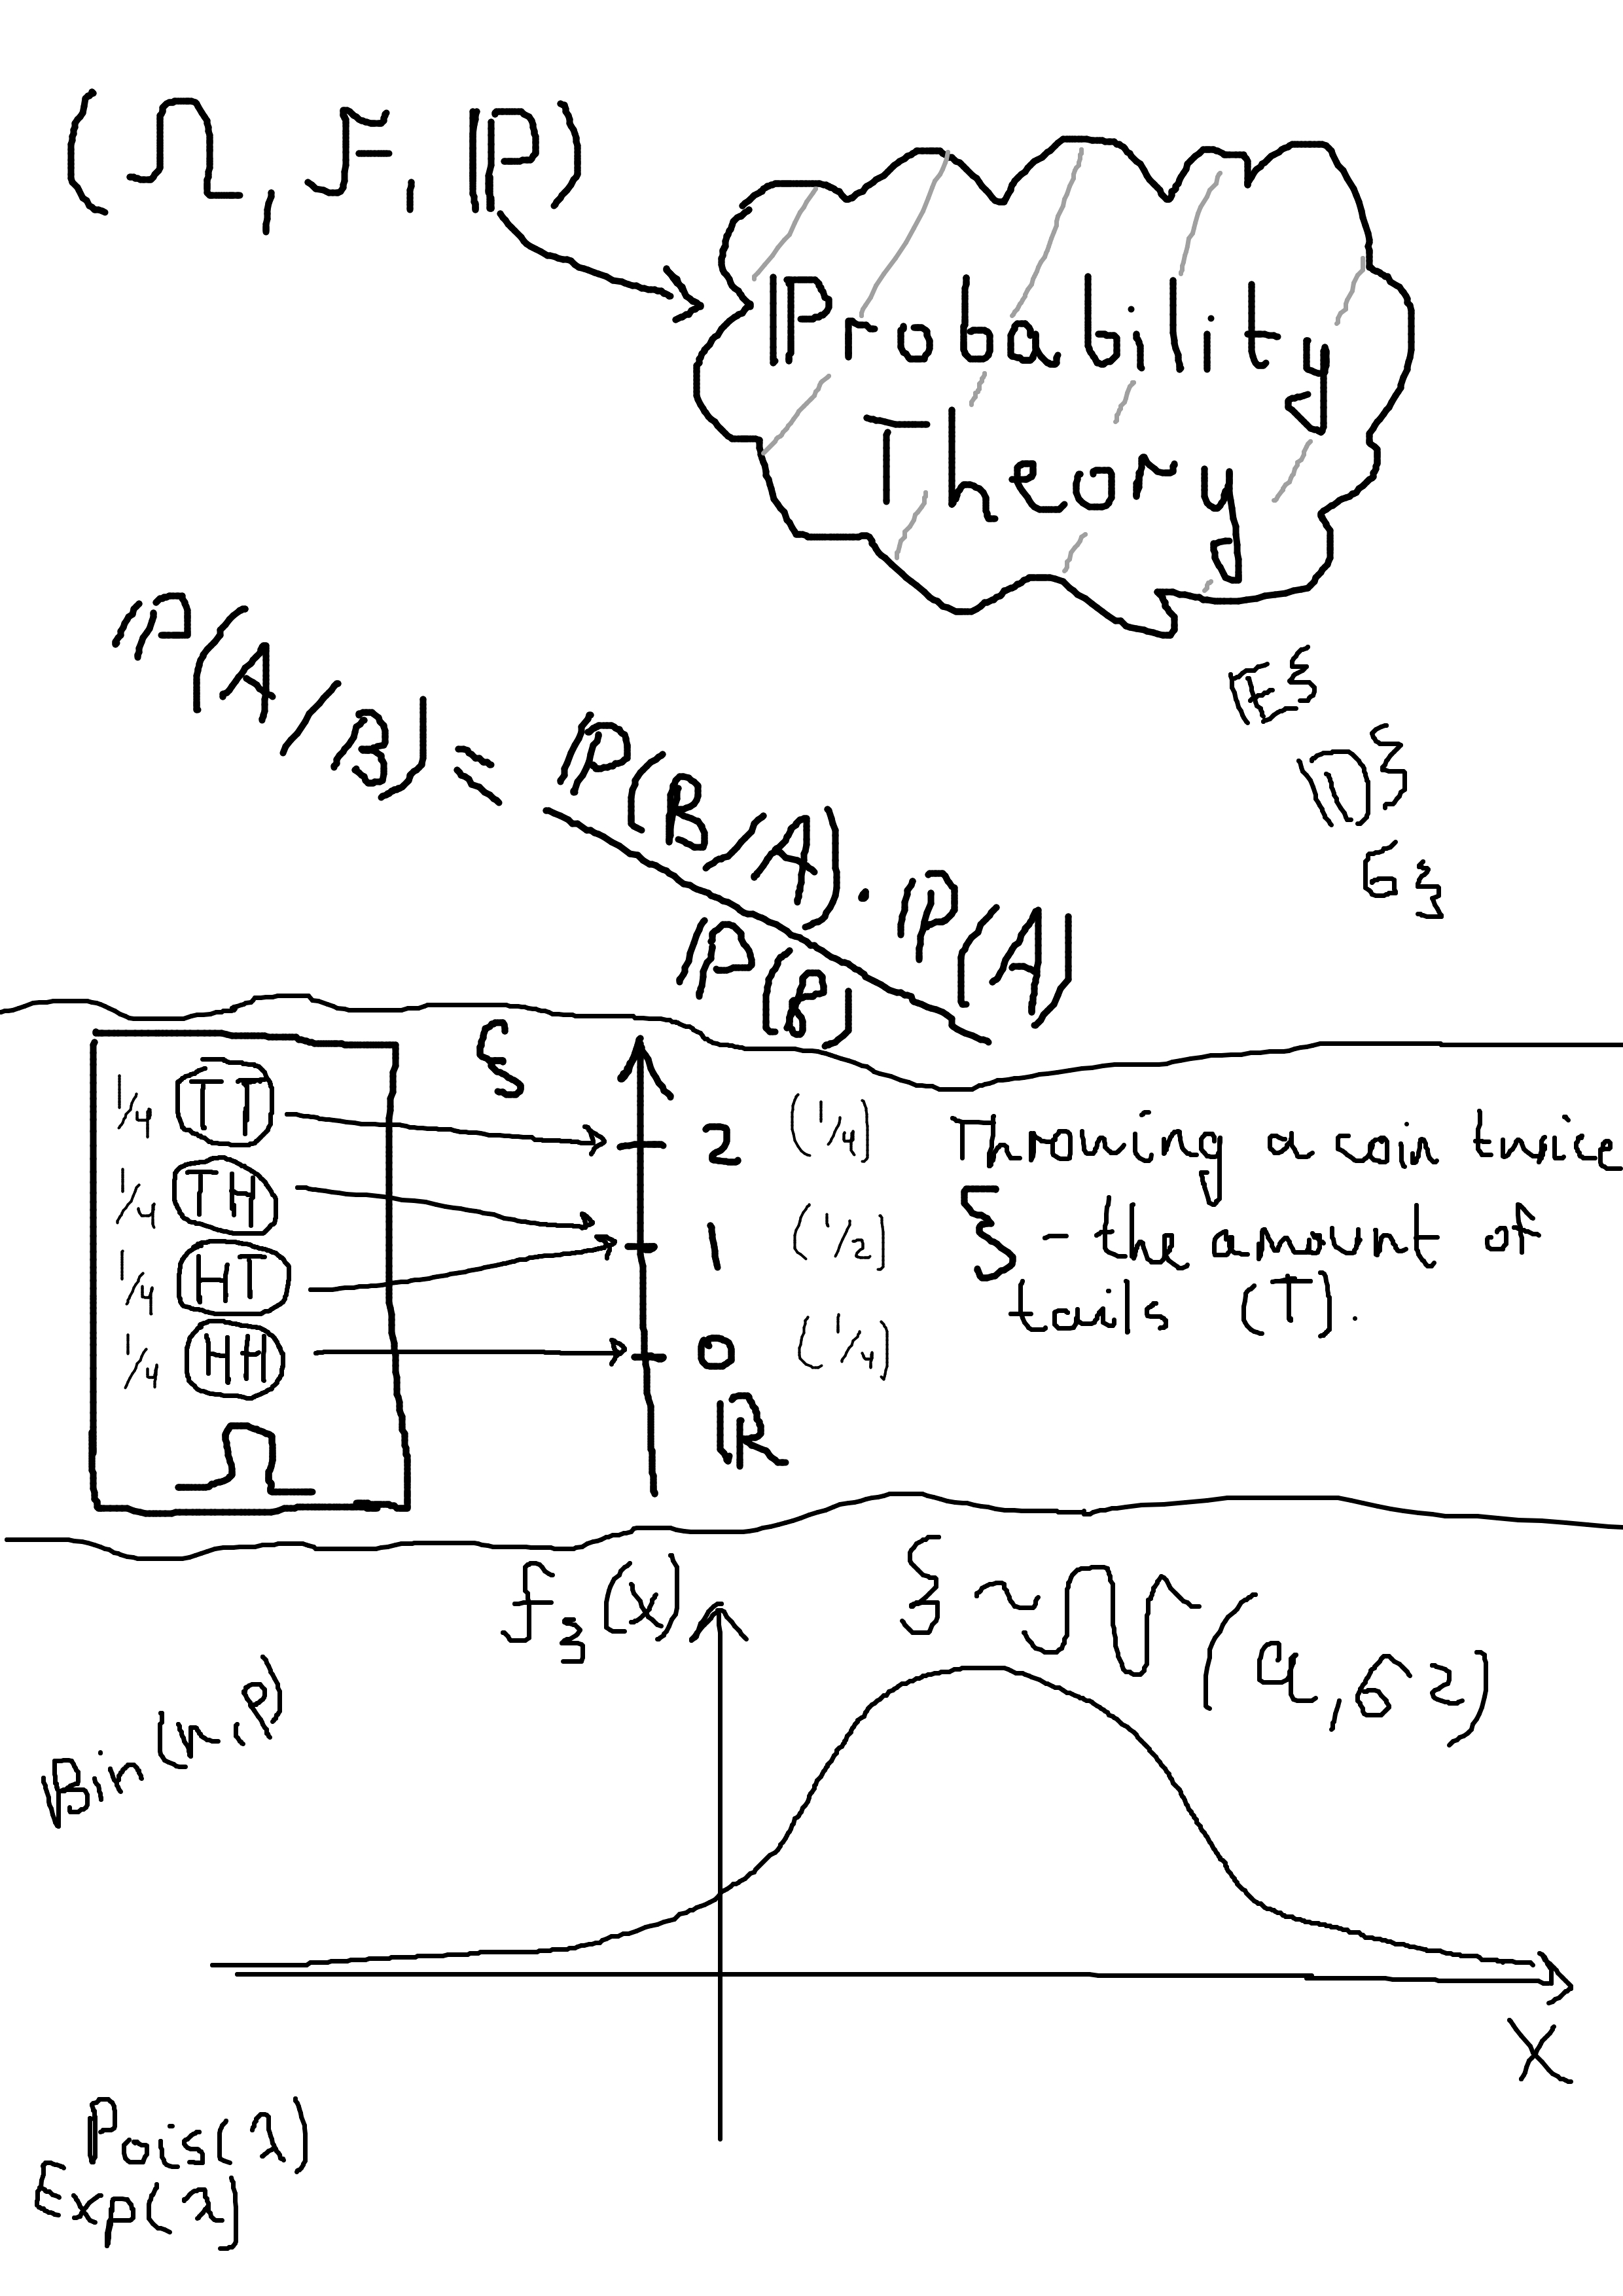
\includepdf[scale=1]{preview.jpg}
\tableofcontents
\newpage
    	
	\section{Лінійні простори}
	\subsection{Основні означення лінійних просторів}
	\begin{definition}\label{vector space}
	\textbf{Лінійним простором} називається множина $L$, на якій задані дві операції:
	\begin{align*}
	\begin{tabular}{cl}
	1. & $\forall x,y \in L: \exists! z \in L: z = x + y$ -- операція додавання \\
	2. & $\forall x \in L, \forall \lambda \in \mathbb{R}: \exists! w \in L: w = \lambda x$ -- операція множення на скаляр \\
	\end{tabular}
	\end{align*}
	та які задовольняють таким аксіомам:
	\begin{align*}
	\begin{tabular}{cl}
	1) & $\forall x,y \in L: x + y = y + x$\\
	2) & $\forall x,y,z \in L: (x + y) + z = x + (y + z)$\\
	3) & $\exists 0 \in L: \forall x \in L: x + 0 = x$\\
	4) & $\forall x \in L: \exists \tilde{x} \in L: x + \tilde{x} = 0$\\
	5) & $\forall \alpha, \beta \in \mathbb{R}: \forall x \in L: (\alpha + \beta) x = \alpha x + \beta x$\\
	6) & $\forall \alpha \in \mathbb{R}: \forall x,y \in L: \alpha (x+y) = \alpha x + \alpha y$\\
	7) & $\forall \alpha, \beta \in \mathbb{R}: \forall x \in L: \alpha (\beta x) = (\alpha \beta) x$\\
	8) & $\forall x \in L: 1 \cdot x = x$
	\end{tabular}
	\end{align*}
	Частіше лінійний простір називають по-іншому: \textbf{векторний простір}.\\
	Всі елементи векторного простору називають часто ще \textbf{векторами}.
	\end{definition}
	
	\begin{remark}
	Якщо $\alpha, \beta \in \mathbb{R}$, то лінійний простір називається  \textbf{дійсним}. При $\mathbb{C}$ -- \textbf{комплексним}.\\
	\textit{Я далі лише буду розглядати дійсні простори, якщо щось додаткове не буде сказано. Для комплексних просторів все буде аналогічно (якщо ніде інше не буде уточнено).}
	\end{remark}
	
	%additional info
	\iffalse
	\begin{remark}
	Да й взагалі-то кажучи, лінійний простір можна визначити на будь-якому полі $F$. Зокрема множини $\mathbb{R}, \mathbb{C}$ самі утворюють поле, але це вже просунута штука.
	\end{remark}
	\fi
	
	\begin{example}
	Розглянемо прості приклади лінійних просторів:
	\begin{enumerate}[nosep, wide=0pt, label={\arabic*)}]
	\item $L = \mathbb{R}^3$ -- вектори в просторі;
	\item $L = \mathbb{R}[x]$ -- многочлени з дійсними коефіцієнтами;
	\item $L = C(A)$ -- неперервні функції на множині $A$.
	\end{enumerate}
	\end{example}
	
	\begin{example}
	Задамо множину $L = \mathbb{R}_{> 0}$, на якій задаються операції таким чином:\\
	$x + y = x \cdot y$ \qquad $\lambda x = x^\lambda$.\\
	Ми доведемо, що утвориться лінійний простір. Дійсно,
	\begin{enumerate}[nosep, wide=0pt, label={\arabic*)}]
	\item $x+y = x \cdot y = y \cdot x = y + x$;
	\item $(x+y) + z = (x \cdot y) + z = (x \cdot y) \cdot z = x \cdot (y \cdot z) = x + (y \cdot z) = x + (y + z)$;
	\item Існує елемент $\textcolor{red}{0} = 1$, для якого $x + 0 = x \cdot 0 = x \cdot 1 = x$. Тут $\textcolor{red}{0}$ -- не число, а символ спеціальний;
	\item Існує елемент $\tilde{x} = \dfrac{1}{x}$, для якого $x + \tilde{x} = x \cdot \tilde{x} = x \cdot \dfrac{1}{x} = 1 = \textcolor{red}{0}$;
	\item $(\alpha + \beta)x = x^{\alpha + \beta} = x^{\alpha} x^{\beta} = \alpha x + \beta x$;
	\item $\alpha (x+y) = (x+y)^\alpha = (xy)^{\alpha} = x^{\alpha} y^{\alpha} = \alpha x + \alpha y$;
	\item $\alpha (\beta x) = \alpha x^\beta = (x^\beta)^\alpha = x^{\alpha \beta} = (\alpha \beta) x$;
	\item $1 \cdot x = x^1 = x$.
	\end{enumerate}
	Всі вісім аксіом виконані. Отже, $L$ -- лінійний простір.
	\end{example}
	
	\begin{proposition}[Властивості лінійних просторів]
	Задано $L$ -- лінійний простір. Тоді виконуються такі пункти:
	\begin{enumerate}[nosep, wide=0pt, label={\arabic*)}]	
	\item існуючий елемент $0 \in L$ -- єдиний;
	\item $\forall x \in L$ існуючий елемент $\tilde{x}$ -- єдиний;
	\item $\underset{\in \mathbb{R}}{0} \cdot x = \underset{\in L}{0}$;
	\item $\tilde{x} = (-1) \cdot x$. Скорочено позначають елемент $(-1) \cdot x = -x$.
	\end{enumerate}
	\end{proposition}
	
	\begin{proof}
	Покажемо виконання кожної властивості.
	\begin{enumerate}[topsep=-\parskip, wide=0pt, label={\arabic*)}]
	\item !Припустимо, що $\exists \tilde{0} \in L: x + \tilde{0} = x$ - ще один нуль. Тоді $\tilde{0} = 0 + \tilde{0} = 0$. Суперечність! Отже, елемент -- єдиний.
	\item !Припустимо, що $\exists \tilde{\tilde{x}} \in L: x + \tilde{\tilde{x}} = 0$ - ще один обернений елемент. Тоді $\tilde{\tilde{x}} = 0 + \tilde{\tilde{x}} = (\tilde{x} + x) + \tilde{\tilde{x}} = \tilde{x} + (x + \tilde{\tilde{x}}) = \tilde{x} + 0 = \tilde{x}$. Суперечність! Отже, елемент -- єдиний.
	\item $0 \cdot x = (0 + 0)x = 0\cdot x + 0 \cdot x \Rightarrow 0 \cdot x = 0$. У нас остання рівність каже, що до елементу $0 \cdot x$ додається щось, що дорівнює $0 \cdot x$. І ось це щось буде рівне $0$.
	\item $x + (-x) = 1 \cdot x + (-1) \cdot x = (1 + (-1))x = 0 \cdot x = 0$.
	\end{enumerate}
	Всі властивості доведені.
	\end{proof}
	
	\begin{remark}
	У разі якщо принаймні одна з властивостей не буде виконаною, то $L$ більше не буде лінійним простором.
	\end{remark}
	
	\begin{example}
	Задамо множину $L = \mathbb{R}^2$, на якій задаються операції таким чином:\\
	$\begin{pmatrix}
	x_1 \\ y_1
	\end{pmatrix} + \begin{pmatrix}
	x_2 \\ y_2
	\end{pmatrix} = \begin{pmatrix}
	x_1 + x_2 \\ y_1+y_2
	\end{pmatrix}$ \quad $\lambda \begin{pmatrix}
	x_1 \\ y_1
	\end{pmatrix} = \begin{pmatrix}
	\lambda x_1 \\ 0
	\end{pmatrix}$.\\
	Можемо зауважити, що $(-1) \begin{pmatrix}
	x_1 \\ y_1
	\end{pmatrix} = \begin{pmatrix}
	-x_1 \\ 0
	\end{pmatrix} \neq \begin{pmatrix}
	-x_1 \\ -y_1
	\end{pmatrix} = - \begin{pmatrix}
	x_1 \\ y_1
	\end{pmatrix}$. Точніше кажучи, рівність виконана лише при $y_1 = 0$, але не для всіх таких векторів. Отже, $L$ -- не лінійний простір. Просто тому що порушується четверта властивість лінійних просторів.
	\end{example}
	
	\subsection{Лінійні підпростори}
	\begin{definition}
	Задано $L$ -- лінійний простір.\\
	Підмножина $M \subset L$ називається \textbf{підпростором}, якщо
	\begin{align*}
	\begin{tabular}{cl}
	1) & $\forall x, y \in M: x + y \in M$\\
	2) & $\forall x \in M: \forall \lambda \in \mathbb{R}: \lambda x \in M$\\
	\end{tabular}
	\end{align*}
	Тобто множина $M$ -- замкнена відносно операцій на $L$.
	\end{definition}
	
	\begin{theorem}
	Задані $L$ -- лінійний простір та $M \subset L$ -- підпростір. Тоді $M$ -- лінійний простір.
	\end{theorem}
	
	\begin{proof}
	На множині $M$ вже задані операції за означенням із простору $L$. Перевіримо всі 8 аксіом. Отже, нехай $x,y,z \in M$, а це автоматично означає $x,y,z \in L$. Також нехай $\alpha,\beta \in \mathbb{R}$. Тоді:
	\begin{enumerate}[wide = 0pt, nosep, label={\arabic*)}]
	\item $x+y=y+x$;
	\item $x+(y+z)=(x+y)+z$;
	\item Оскільки $x \in M$, то звідси $0\cdot x \in M$, а тому $0 \cdot x \in L$, але оскільки $L$ -- лінійний простір, то за властивістю 3), $0 \cdot x = 0$, а також звідси $0 + x = 0$;
	\item Оскільки $x \in M$, то звідси $(-1) \cdot x \in M$, а тому $(-1) \cdot x \in L$, але оскільки $L$ -- лінійний простір, то за властивістю 4), $(-1) \cdot x = -x$, а також звідси $x + (-x) = 0$;
	\item $(\alpha + \beta)x = \alpha x + \beta x$;
	\item $\alpha (x+y)= \alpha x + \alpha y$;
	\item $(\alpha \beta) x = \alpha (\beta x)$;
	\item $1 \cdot x = 1$.
	\end{enumerate}
	Отже, $M$ -- лінійний простір за означенням.
	\end{proof}

	\begin{example}	
		$M = \mathbb{R}_n[x]$ -- многочлен степені не більший за $n$ -- підпростір лінійного простору $L = \mathbb{R}[x]$. Тому $M = \mathbb{R}_n[x]$ є також лінійним простором.
	\end{example}
	
	\subsection{Лінійна залежність та лінійна незалежність}
	\begin{definition}
	Задано $L$ -- лінійний простір.\\
	Система елементів $\{x_1, \dots, x_n\} \subset L$ називається \textbf{лінійно незалежною (л.н.з.)}, якщо
	\begin{align*}
	\alpha_1 x_1 + \dots + \alpha_n x_n = 0 \implies \alpha_1 = \dots = \alpha_n = 0.
	\end{align*}
	Система елементів $\{x_1, \dots, x_n\} \subset L$ називається \textbf{лінійно залежною (л.з.)}, якщо
	\begin{align*}
	\exists \alpha_1,\dots,\alpha_n \in \mathbb{R}: |\alpha_1| + \dots + |\alpha_n| \neq 0: \alpha_1 x_1 + \dots + \alpha_n x_n = 0.
	\end{align*}
	\end{definition}
	
	\begin{remark}
	Означення лінійної залежності записане як заперечення лінійної незалежності.
	\end{remark}
	
	\begin{remark}
	Вираз $|\alpha_1| + \dots + |\alpha_n| \ne 0$ по-українськи можна трактувати як "не всі $\alpha_i$ нулеві".
	\end{remark}
	
	\begin{definition}
	\textbf{Лінійною комбінацією} елементів $y_1,\dots,y_n$ називається вираз
	\begin{align*}
	\gamma_1 y_1 + \dots + \gamma_n y_n,
	\end{align*}
	де $\gamma_1, \dots, \gamma_n \in \mathbb{R}$.
	\end{definition}
	
	\begin{example}
	Будь-які вектори $\{\vec{a}, \vec{b} \}$ -- л.н.з.\ в $\mathbb{R}^2 \iff $ вони не колінеарні (див.\ аналітичну геометрію).
	\end{example}
	
	\begin{example}
	Заданий лінійний простір $L = \mathbb{R}^4$ і система векторів $\{\vec{x}_1,\vec{x}_2,\vec{x}_3,\vec{x}_4\}$, де\\
	$\vec{x}_1 =\begin{pmatrix} 1\\ 0\\ 2\\ 3 \end{pmatrix},\ \vec{x}_2 =\begin{pmatrix} 4\\ -1\\ 2\\ 1 \end{pmatrix},\ \vec{x}_3 =\begin{pmatrix} 2\\ 1\\ -1\\ 3 \end{pmatrix},\ \vec{x}_4 =\begin{pmatrix} 1\\ -2\\ 1\\ -5 \end{pmatrix}$.\\
	Перевіримо, чи буде система $\{\vec{x}_1,\vec{x}_2,\vec{x}_3,\vec{x}_4\}$ л.н.з. Розпишемо їхню лінійну комбінацію:\\
	$\alpha_1 \vec{x}_1 + \alpha_2 \vec{x}_2 + \alpha_3 \vec{x}_3 + \alpha_4 \vec{x}_4 = \vec{0}$.\\
	$\alpha_1 \begin{pmatrix} 1\\ 0\\ 2\\ 3 \end{pmatrix} + \alpha_2 \begin{pmatrix} 4\\ -1\\ 2\\ 1 \end{pmatrix} + \alpha_3 \begin{pmatrix} 2\\ 1\\ -1\\ 3 \end{pmatrix} + \alpha_4 \begin{pmatrix} 1\\ -2\\ 1\\ -5 \end{pmatrix} = \begin{pmatrix} 0\\ 0\\ 0\\ 0 \end{pmatrix}$.\\
	Дане рівняння можна записати в вигляді системи рівнянь:\\
	$\begin{cases}
	(1): \alpha_1 + 4\alpha_2 + 2\alpha_3 + \alpha_4 = 0\\
	(2): -\alpha_2 + \alpha_3 - 2\alpha_4 = 0\\
	(3): 2\alpha_1 + 2\alpha_2 - \alpha_3 + \alpha_4 = 0\\
	(4): 3\alpha_1 + \alpha_2 + 3\alpha_3 - 5\alpha_4 = 0
	\end{cases} \implies \begin{cases}
	(1): & \alpha_1 + 4\alpha_2 + 2\alpha_3 + \alpha_4 = 0\\
	(2): & \alpha_2 - \alpha_3 + 2\alpha_4 = 0\\
	(3)-2(1): & 6\alpha_2 + 5\alpha_3 + \alpha_4 = 0\\
	(4)-3(1): & 11\alpha_2 + 3\alpha_3 + 8\alpha_4 = 0
	\end{cases}$\\
	
	$\implies \begin{cases}
	(1): & \alpha_1 + 4\alpha_2 + 2\alpha_3 + \alpha_4 = 0\\
	(2): & \alpha_2 - \alpha_3 + 2\alpha_4 = 0\\
	-6(2)+(3): & 11\alpha_3 - 11\alpha_4 = 0\\
	-11(4)+(4): & 14\alpha_3 - 14\alpha_4 = 0
	\end{cases} 
	\implies
	\begin{cases}
	\alpha_1 = 9\alpha_4\\
	\alpha_2 = -3\alpha_4\\
	\alpha_3 = \alpha_4
	\end{cases} 
	$.\\
	Звісно, є нульовий розв'язок, але такий розв'язок не буде єдиним. Можна взяти $(9,-3,1,1)$, щоб наша лінійна комбінація елементів $\vec{x}_1,\vec{x}_2,\vec{x}_3,\vec{x}_4$ була нулевою. Отже, $\{\vec{x}_1,\vec{x}_2,\vec{x}_3,\vec{x}_4\}$ -- л.з.
	\end{example}
	
	\begin{example}
	Перевіримо, чи буде $\{\sin x, \cos x, \cos 2x\}$ -- л.н.з.\ в лінійному просторі $L = C(\mathbb{R})$.\\
	$\alpha_1 \sin x + \alpha_2 \cos x + \alpha_3 \cos 2x = 0(x)$, причому виконано $\forall x \in \mathbb{R}$. Тут типу $0(x) = 0,\ \forall x \in \mathbb{R}$.\\
	Якщо ця рівність виконується для довільних $x$, то зокрема має виконуватись і для конкретних.\\
	При $x = 0$ отримаємо $\alpha_2 + \alpha_3 = 0$.\\
	При $x = \dfrac{\pi}{2}$ отримаємо $\alpha_1 - \alpha_3 = 0$.\\
	При $x = \dfrac{\pi}{4}$ отримаємо $\dfrac{\sqrt{2}}{2} \alpha_1 + \dfrac{\sqrt{2}}{2} \alpha_2 = 0$.\\
	Отже, виникає система, яка має одночасно виконуватися:\\
	$\begin{cases}
	\alpha_2 + \alpha_3 = 0\\
	\alpha_1 - \alpha_3 = 0\\
	\alpha_1 + \alpha_2 = 0
	\end{cases}
	\implies
	\begin{cases}
	\alpha_2 =  -\alpha_3\\
	\alpha_1 = \alpha_3\\
	\end{cases}
	$\\
	Тут вже можуть виникати думки, що це -- л.з.\ система, але (!) візьмемо ще один $\displaystyle x = \frac{\pi}{3}: \\ \frac{\sqrt{3}}{2}\alpha_1 + \frac{1}{2}\alpha_2 + \frac{1}{2}\alpha_3 = 0$.\\
	У це рівняння підставимо отримані $\alpha_1,\alpha_2$ -- маємо наступне:\\
	$\sqrt{3}\alpha_3 - \alpha_3 + \alpha_3 = 0 \implies \alpha_3 = 0$. А отже, $\alpha_1 = \alpha_2 = 0$.\\
	Тобто щоб виконувались всі чотири рівняння одночасно, треба обов'язково $\alpha_1 = \alpha_2 = \alpha_3 = 0$.\\
	Якщо підставляти абсолютно інші $x \in \mathbb{R}$, то ми отримаємо деяке рівняння, яке автоматично виконано в силу того, що $\alpha_1,\alpha_2,\alpha_3 = 0$.\\
	Остаточно: $\{\sin x, \cos x, \cos 2x\}$ -- л.н.з.
	\end{example}
	
	\begin{remark}
	Тут не можна використовувати цю тотожність: $\cos 2x = \cos ^2 x - \sin ^2 x$. Тому що тут фігурує степінь "квадрат": нема множення двох елементів у лінійному просторі (лише множення на скаляр), $\cos^2 x$ або $\sin^2 x$ -- це вже абсолютно інший елемент.
	\end{remark}
	
	\begin{proposition}[Властивості л.з.\ систем]
	Заданий $L$ -- лінійний простір та система $\{x_1,\dots,x_n\}$. Тоді виконуються такі пункти:
	\begin{enumerate}[nosep, wide = 0pt, label={\arabic*)}]
	\item Якщо система містить л.з.\ підсистему $\{x_{j_1} \dots, x_{j_k}\}$, то вся система $\{x_1,\dots,x_n\}$ л.з.;
	\item Якщо $\{x_1 \dots, x_n\}$ містить принаймні один нульовий елемент, то ця система -- л.з.;
	\item Система $\{x_1 \dots, x_n\}$ -- л.з. $\iff$ існує елемент системи, який можна виразити як лінійну комбінацію від всіх інших.
	\end{enumerate}
	\end{proposition}
	
	\begin{proof}
	Покажемо виконання кожної властивості.
	\begin{enumerate}[topsep=-\parskip, wide=0pt, label={\arabic*)}]
	\item $\{x_{j_1} \dots, x_{j_k}\}$ -- л.з., тобто $\exists \alpha_1, \dots, \alpha_k$ ненулеві: $\alpha_1 x_{j_1} + \dots + \alpha_k x_{j_k} = 0$. Звідси випливає, що:\\
	$0x_1 + 0x_2 + \dots + 0x_{j_1-1} + \alpha_1 x_{j_1} + 0x_{j_1 + 1} + \dots + \alpha_k x_{j_k} + \dots + 0 x_n = 0$.\\
	Деякі коефіцієнти в новій лінійнії комбінації ненулеві. Отже, $\{x_1 \dots, x_n\}$ -- л.з.
	\item Припустимо, що $x_j = 0$, маємо лінійну комбінацію $\alpha_1 x_1 + \dots + \alpha_j \underset{=0}{x_j} + \alpha_n x_n = 0$. Можна взяти $\alpha_1 = \dots = \alpha_n = 0$, але $\alpha_j = 1$. Тому наша система буде л.з.
	\item В обидва боки доведення.\\
	\rightproof Дано: $\{x_1, \dots, x_n\}$ -- л.з., тобто $\exists \beta_1, \dots, \beta_n$ не всі нулеві: $\beta_1 x_1 + \dots + \beta_n x_n = 0$.\\
	Не всі нулеві, тобто $\exists \beta_j \neq 0$. Тоді
	$\beta_j x_j = -\beta_1 x_1 - \dots - \beta_{j-1} x_{j-1} - \beta_{j+1} x_{j+1} - \dots - \beta_n x_n$.\\
	$\displaystyle x_j = \frac{-\beta_1}{\beta_j}x_1 - \dots - \frac{-\beta_n}{\beta_j}x_n$. А це є розклад в лінійну комбінацію інших.
	\bigskip \\
	\leftproof Дано: $\exists x_j: \exists \alpha_1, \dots, \alpha_{j-1}, \alpha_{j+1}, \dots, \alpha_n: x_j = \alpha_1 x_1 + \dots + \alpha_{j-1} x_{j-1} + \alpha_{j+1} x_{j+1} + \dots + \alpha_n x_n$.\\
	$\implies \alpha_1 x_1 + \dots + \alpha_{j-1} x_{j-1} + (-1)x_j + \alpha_{j+1} x_{j+1} + \dots + \alpha_n x_n = 0$.\\
	Коефіцієнти не всі нулеві. Отже, $\{x_1, \dots, x_n\}$ -- л.з.
	\end{enumerate}
	Всі властивості доведені.
	\end{proof}
	
	\begin{proposition}[Властивості л.н.з.\ систем]
	Задано $L$ -- лінійний простір та система $\{x_1,\dots,x_n\}$. Тоді виконуються такі пункти:
	\begin{enumerate}[nosep, wide = 0pt, label={\arabic*)}]
	\item Якщо система $\{x_1, \dots, x_n\}$ л.н.з., то будь-яка підсистема теж л.н.з.;
	\item Нехай $y \in L$ та є лінійною комбінацією елементів системи, тобто $y = \alpha_1 x_1 + \dots + \alpha_n x_n$. Тоді $\{x_1, \dots, x_n\}$ -- л.н.з. $\iff$ розклад елемента $y$ є єдиним.
	\end{enumerate}
	\end{proposition}
	
	\begin{proof}
	Покажемо виконання кожної властивості.
	\begin{enumerate}[topsep=-\parskip, wide=0pt, label={\arabic*)}]
	\item \textit{наслідок властивості 1) попереднього твердженння.}
	\item В обидва боки доведення.\\
	\rightproof Дано: $\{x_1, \dots, x_n \}$ -- л.н.з.\\
	!Припустимо, що розклад не є єдиним. Тобто існує ще одна лінійна комбінація для елемента $y$, тобто $y = \beta_1 x_1 + \dots + \beta_n x_n$. Тоді:\\
	$0 = y - y = (\alpha_1 - \beta_1)x_1 + \dots + (\alpha_n - \beta_n)x_n$.\\
	Але з умови л.н.з. випливає, що $\alpha_1 = \beta_1, \dots, \alpha_n = \beta_n$. Суперечність! \\ 
	Отже, в лінійну комбінацію елементу $y$ розкладається єдиним чином.
	\bigskip \\
	\leftproof Дано: $\exists! \alpha_1, \dots, \alpha_n:$
	$y = \alpha_1 x_1 + \dots + \alpha_n x_n$. Перевіримо систему $\{x_1, \dots, x_n\}$ на л.н.з.\\
	$\gamma_1 x_1 + \dots + \gamma_n x_n = 0$.\\
	$y = y + 0 = (\alpha_1 + \gamma_1)x_1 + \dots + (\alpha_n + \gamma_n)x_n$\\
	Але за умовою розклад єдиний, тому $\alpha + \gamma_1 = \alpha_1, \dots, \alpha_n + \gamma_n = \alpha_n \implies \gamma_1 = \dots = \gamma_n = 0$.\\
	Отже, система $\{x_1,\dots,x_n\}$ -- л.н.з.
	\end{enumerate}
	Всі властивості доведені.
	\end{proof}
	
	\subsubsection*{Елементарні перетворення л.н.з.\ та л.з.\ систем}
	Задано лінійний простір $L$ та систему $\{x_1, \dots, x_n\}$. Її можна трохи видозмінити трьома перетвореннями: $P_{j \leftrightarrow k},\ P_{j \to \lambda j},\ P_{j \to j+k}$. Під час дії цих перетворень на систему вони роблять наступне:
	\begin{enumerate}[wide = 0pt, label={\Roman*.}]
	\item $P_{j \leftrightarrow k} \{x_1, \dots, x_j, \dots, x_k, \dots, x_n\} = \{x_1, \dots, x_k, \dots, x_j, \dots, x_n\}$\\
	$j$-ий та $k$-ий елементи зміняться місцями.
	\item $P_{j \to \lambda j} \{x_1, \dots, x_j, \dots, x_n\} = \{x_1, \dots, \lambda x_j, \dots, x_n\}$\\
	до $j$-го елементу множимо скаляр, тільки якщо $\lambda \neq 0$.
	\item $P_{j \to j+k} \{x_1, \dots, x_j, \dots, x_k, \dots, x_n\} = \{x_1, \dots, x_j, \dots,  x_k + x_j, \dots, x_n\}$\\
	до $j$-го елементу додаємо $k$-ий елемент.
	\end{enumerate}

	\begin{proposition}
	Перетворення I, II та III зберігають лінійну залежність чи незалежність.
	\end{proposition}
	
	\begin{proof}
	Доведемо спочатку випадок л.н.з. Маємо початкову систему $\{x_1, \dots, x_n\}$ -- л.н.з. Розглянемо кожне перетворення:
	\begin{enumerate}[wide = 0pt, label={\Roman*.}]
	\item $P_{j \leftrightarrow k}\{x_1, \dots, x_j, \dots, x_k \dots, x_n\} = \{x_1, \dots, x_k, \dots, x_j \dots, x_n\}$.\\
	$\alpha_1 x_1 + \dots + \alpha_j x_k + \dots + \alpha_k x_j + \dots + \alpha_n x_n = 0 \overset{\text{початкова -- л.н.з.}}{\implies} \alpha_1 = \dots = \alpha_n = 0$.
	\item $P_{j \to \lambda j}\{x_1, \dots, x_j, \dots, x_n\} = \{x_1, \dots, \lambda x_j, \dots, x_n\}$.\\
	$\alpha_1 x_1 + \dots + \alpha_j \lambda x_j + \dots + \alpha_n x_n = 0 \overset{\text{початкова -- л.н.з.}}{\implies} \alpha_1 = \dots = \alpha_j \lambda = \dots = \alpha_n = 0$. Але оскільки $\lambda \neq 0$, то гарантовано $\alpha_j = 0$.
	\item $P_{j \to j+k}\{x_1, \dots, x_j, \dots, x_k, \dots, x_n\} = \{x_1, \dots, x_j, \dots,  x_k + x_j, \dots, x_n\}$.\\
	$\alpha_1 x_1 + \dots + \alpha_j x_j + \dots + \alpha_k(x_k + x_j) + \dots + \alpha_n x_n = 0 \implies \\ \alpha_1 x_1 + \dots + (\alpha_k + \alpha_j) x_j + \dots + \alpha_k x_k + \dots + \alpha_n x_n = 0 \overset{\text{початкова -- л.н.з.}}{\implies} \\ \alpha_1 = \alpha_j + \alpha_k = \dots = \alpha_k = \dots = \alpha_n = 0$. Тоді $\alpha_j = 0$.
	\end{enumerate}
	Отже, л.н.з. система після будь-якого елементарного перетворення залишається л.н.з.
	\bigskip \\
	Залишилось довести випадок л.з. Мамємо початкову систему $\{x_1,\dots,x_n\}$ -- л.з.\\
	!Припустимо, що л.з. система після будь-якого з трьох перетворення стане л.н.з. Тобто система $P_{\textrm{будь-яке}} \{x_1, \dots, x_n\}$ -- л.н.з. Зробимо зворотне перетворення (щоб повернути систему так, як вона виглядала) в залежності від того, яке перетворення використовували (I,II або III), тобто:
	\begin{enumerate}[nosep, wide = 0pt, label={\Roman*.}]
	\item $\{x_1,\dots,x_k, \dots, x_j, \dots,x_n\}$ -- змінити ще раз $j$-ий,$k$-ий елементи місцями (це буде $P_{j \leftrightarrow k})$);
	\item $\{x_1, \dots, \lambda x_j, \dots, x_n\}$ -- помножити на $\dfrac{1}{\lambda}$ $j$-ий елемент (це буде $P_{j \to \frac{1}{\lambda} j}$);
	\item $\{x_1, \dots, x_j, \dots,  x_k + x_j, \dots, x_n\}$ -- помножити на $(-1)$ елемент $x_j$, додати $j$-ий елемент до елементу $x_k+x_j$, а потім помножити на $(-1)$ елемент $(-x_j)$ (це буде $P_{j \to (-1)j}$, далі $P_{j \to k+j}$, а потім $P_{j \to (-1)j}$).
	\end{enumerate}
	Отримаємо початкову систему, що має стати л.н.з., згідно з щойно доведеним випадком. А ми маємо л.з. за умовою, тому суперечність! \\
	Отже, л.з. система після елементарного перетворення залишається л.з.
	\end{proof}
	
	\begin{example}
	Задано систему векторів $\{\vec{x}_1,\vec{x}_2,\vec{x}_3\}$ в лінійному просторі $\mathbb{R}^3$. Перевірити, чи буде вона л.н.з., де \\ $\vec{x}_1 = \begin{pmatrix}
	14 \\ -27 \\ -49 \\ 113
	\end{pmatrix},\ \vec{x}_2 = \begin{pmatrix}
	43 \\ -82 \\ -145 \\ 340
	\end{pmatrix},\ \vec{x}_3 = \begin{pmatrix}
	85 \\ -163 \\ -293 \\ 677
	\end{pmatrix}$.\\
	Зробимо такі перетворення над системою: $\{\vec{x}_1, \vec{x}_2 - 3 \vec{x}_1, \vec{x}_3 - 6\vec{x}_1 \}$. Позначу їх як $\{\vec{x}^*_1,\vec{x}^*_2,\vec{x}^*_3\}$, де\\
	$\vec{x}^*_1 = \vec{x}_1 = \begin{pmatrix}
	14 \\ -27 \\ -49 \\ 113
	\end{pmatrix},\ \vec{x}^*_2 = \vec{x}_2 - 3\vec{x}_1 = \begin{pmatrix}
	1 \\ -1 \\ 2 \\ 1
	\end{pmatrix},\ \vec{x}^*_3 = \vec{x}_3 - 6\vec{x}_1 = \begin{pmatrix}
	1 \\ -1 \\ 1 \\ -1
	\end{pmatrix}$.\\
	Розпишемо їхню лінійну комбінацію -- отримаємо:\\
	$\alpha_1 \vec{x}^*_1 + \alpha_2 \vec{x}^*_2 + \alpha_3 \vec{x}^*_3 = \vec{0} \implies \begin{cases} 14 \alpha_1 + \alpha_2 + \alpha_3 = 0 \\
					   -27 \alpha_1 - \alpha_2 - \alpha_3 = 0 \\
					   113 \alpha_1 + \alpha_2 - \alpha_3 = 0
	\end{cases} \implies \alpha_1 = 0, \alpha_2 = 0, \alpha_3 = 0$.\\
	Таким чином, $\{\vec{x}^*_1, \vec{x}^*_2, \vec{x}^*_3\}$ -- л.н.з., а тому початкова система $\{\vec{x}_1,\vec{x}_2,\vec{x}_3\}$ -- л.н.з.
	\end{example}
	
	\subsection{Лінійні оболонки}
	\begin{definition}
	Задано $L$ -- лінійний простір і система $\{x_1, \dots, x_n\} \subset L$.\\
	\textbf{Лінійною оболонкою} цієї системи називають множину всіх лінійних комбінацій:
	\begin{align*}
	\linspan\{x_1, \dots, x_n\} = \{\alpha_1 x_1 + \dots + \alpha_n x_n \mid \alpha_1, \dots, \alpha_n \in \mathbb{R}\}
	\end{align*}
	Інколи ще позначають $\text{л.о.}\{x_1,\dots,x_n\}$ в нашій літературі. Я дотримуватимусь першого позначення.\\
	Якщо взяти довільну множину $M \subset L$, то \textbf{лінійна оболонка} множини задається таким чином:
	\begin{align*}
	\linspan M = \{\alpha_1 x_1 + \dots + \alpha_j x_j \mid j \geq 1,\ x_1,\dots,x_j \in M,\ \alpha_1, \dots, \alpha_j \in \mathbb{R}\}
	\end{align*}
	\end{definition}
	
	\begin{proposition}
	Задано $L$ -- лінійний простір. Тоді лінійна оболонка (системи або множини) є підпростором.
	\end{proposition}
	
	\begin{proof}
	Доведення за означенням. Нехай є $\linspan\{x_1, \dots, x_n\}$. Маємо, що $\forall w_1, w_2 \in \linspan\{x_1, \dots, x_n\}$, тобто:\\
	$w_1 = \alpha_1 x_1 + \dots + \alpha_n x_n$\\
	$w_2 = \beta_1 x_1 + \dots + \beta_n x_n$\\
	$w_1 + w_2 = (\alpha_1 + \beta_1)x_1 + \dots + (\alpha_n + \beta_n)x_n \implies w_1 + x_2 \in \linspan\{x_1, \dots, x_n\}$\\
	$\lambda w_1 = \lambda \alpha_1 x_1 + \dots + \lambda \alpha_n x_n \implies \lambda w_1 \in \linspan\{x_1, \dots, x_n\}$.\\
	Отже, $\linspan\{x_1, \dots, x_n\}$ задає підпростір $L$. Випадок для $\linspan M$ є аналогічним.
	\end{proof} 
	
	\begin{proposition}
	Задано $L$ -- лінійний простір та систему $\{x_1,\dots,x_n\} \subset L$. Тоді $\linspan \{x_1,\dots,x_n \}$ -- найменший підпростір, що містить елементи системи.
	\end{proposition}
	\noindent
Математично кажучи, припустимо, що $K$ -- лінійний підпростір, що містить $x_1,\dots,x_n$ та при цьому $K \subset \linspan \{x_1,\dots,x_n \}$. Тоді $K = \linspan \{x_1,\dots,x_n \}$.\\
	\textit{Вказівка: показати, що} $w \in \linspan\{x_1,\dots,x_n \} \iff w \in K$.
	
	\begin{proposition}
	Задано $L$ -- лінійний простір та множину $M \subset L$. Тоді $\linspan M$ -- найменший підпростір, що містить множину $M$.\\
	\textit{Аналогічно.}
	\end{proposition}
	
	\begin{corollary}
	Якщо $M$ -- лінійний підпростір $L$, то $\linspan M = M$.
	\end{corollary}
	
	\begin{example}
	\label{find_span_of_elements}
	Задано $L = \mathbb{R}^3$ і система з трьох векторів $\{\vec{e}_1,\vec{e}_2,\vec{e}_3\}$, де:\\
	$\vec{e}_1 =\begin{pmatrix} 1\\ 0\\ 0 \end{pmatrix}, \quad \vec{e}_2 =\begin{pmatrix} 0\\ 1\\ 0 \end{pmatrix}, \quad \vec{e}_3 =\begin{pmatrix} 0\\ 0\\ 1 \end{pmatrix}$.\\
	Довести, що $\linspan\{\vec{e}_1, \vec{e}_2, \vec{e}_3\} = \mathbb{R}^3$.\\
	$\linspan\{\vec{e}_1, \vec{e}_2, \vec{e}_3\} \overset{\text{def.}}{=} \{\alpha_1 \vec{e}_1 + \alpha_2 \vec{e}_2 + \alpha_3 \vec{e}_3 \mid \alpha_1, \alpha_2, \alpha_3 \in \mathbb{R}\} = \{(\alpha_1, \alpha_2, \alpha_3)^T \mid \alpha_1, \alpha_2, \alpha_3 \in \mathbb{R}\} = \mathbb{R}^3$.
	\end{example}
	
	\iffalse
	\begin{remark}
	Трошки англійського означення. Там кажуть, що system $\{ x_n,\dots,x_n \}$ \textbf{spans} vector space $L$, if $\{x_1,\dots,x_n\} = L$. Адаптивного перекладу цього поки не знаю.
	\end{remark}
	\fi
		
	\subsection{Підпорядковані та еквівалентні системи}
	\begin{definition}
	Задано $L$ -- лінійний простір.\\
	Система $\{y_1, \dots, y_n \} \subset L$ називається \textbf{підпорядкованою системою} під $\{x_1, \dots, x_m\} \subset L$, якщо:
	\begin{align*}
	\forall y_j: \exists \alpha^j_1, \dots, \alpha^j_m: y_j = \alpha^j_1 x_1 + \dots + \alpha^j_m x_m
	\end{align*}
	Позначення: $\{y_1, \dots, y_n \} \prec \{x_1, \dots, x_m \}$.\\
	Якщо маємо множину $Y \subset L$, то вона називається \textbf{підпорядкованою} під $X \subset L$, якщо:
	\begin{align*}
	\forall y \in Y: \exists x_1,\dots,x_n \in X: \exists \alpha_1, \dots, \alpha_n \in \mathbb{R}: y = \alpha_1 x_1 + \dots + \alpha_n x_n
	\end{align*}
	Позначення: $Y \prec X$.
	\end{definition}
	
	\begin{proposition}
	\label{subordinate_prp1}
	Задано $L$ -- лінійний простір та системи $\{x_1,\dots,x_m\},\ \{y_1,\dots,y_n\} \subset L$.\\
	$\{y_1, \dots, y_n \} \prec \{x_1, \dots, x_m \} \iff \linspan \{y_1, \dots, y_n\} \subset \linspan \{x_1, \dots, x_m \}$.
	\end{proposition}
	
	\begin{proof}
	\rightproof Дано: $\{y_1, \dots, y_n \} \prec \{x_1, \dots, x_m \}$, тобто за означенням:\\
	$\forall y_j: \exists \alpha^j_1, \dots, \alpha^j_m: y_j = \alpha^j_1 x_1 + \dots + \alpha^j_m x_m \Rightarrow y_j \in \linspan\{x_1, \dots, x_m\}$.\\
	$\forall w \in \linspan\{y_1, \dots, y_n\}$, тобто $w = \beta_1 y_1 + \dots + \beta_n y_n \implies w \in \linspan\{x_1, \dots, x_m\}$\\
	Тобто маємо $\linspan \{y_1, \dots, y_n\} \subset \linspan \{x_1, \dots, x_m \}$.
	\bigskip \\
	\leftproof Дано: $\linspan \{y_1, \dots, y_n\} \subset \linspan \{x_1, \dots, x_m \}$.\\
	$\implies \forall y_j \in \linspan \{y_1, \dots, y_n \}$ \hspace{0.2cm}(тому що $y_j = 0y_1 + \dots + 1 y_j + \dots + 0 y_n$)\hspace{0.2cm} $\implies y_j \in \linspan\{x_1,\dots,x_m\}$:\\
	$\exists \alpha^j_1, \dots, \alpha^j_m: y_j = \alpha^j_1 x_1 + \dots + \alpha^j_m x_m$.\\
	Таким чином, маємо $\{y_1, \dots, y_n \} \prec \{x_1, \dots, x_m \}$.
	\end{proof}
	
	\begin{proposition}
	Задано $L$ -- лінійний простір та множини $X,Y \subset L$.\\
	$Y \prec X \iff \linspan Y \subset \linspan X$.\\
	\textit{Аналогічне доведення.}
	\end{proposition}
	
	\begin{proposition}[Властивості підпорядкованих систем]
	\label{subordinate_properties}
	Підпорядкованість систем (або множин) задає відношення порядку. Тобто відношення: рефлексивне, антисиметричне і транзитивне.\\
	\textit{Випливає частково з попереднього твердження.}
	\end{proposition}
	
	\begin{example}
	Нехай задано систему векторів $\{\vec{x}_1,\vec{x}_2,\vec{x}_3\}$ та $\{\vec{y}_1,\vec{y}_2,\vec{y}_3\}$ з $\mathbb{R}^3$, де:\\
	\begin{tabular}{ll}
	$\vec{y}_1 = (0,0,1)$ & $\vec{x}_1 = (1,0,0)$ \\
	$\vec{y}_2 = (0,1,0)$ & $\vec{x}_2 = (1,1,0)$ \\
	$\vec{y}_3 = (1,0,0)$ & $\vec{x}_3 = (1,1,1)$
	\end{tabular}
	\\
	Перевірити, чи можна вважати, що $\{\vec{y}_1, \vec{y}_2, \vec{y}_3 \} \prec \{\vec{x}_1, \vec{x}_2, \vec{x}_3\}$ та одночасно $\{\vec{x}_1, \vec{x}_2, \vec{x}_3\} \prec \{\vec{y}_1, \vec{y}_2, \vec{y}_3\}$.\\
	Розв'яжемо задачу на основі доведеного твердження.\\
	Ми вже знаємо, що $\linspan\{\vec{y}_1,\vec{y}_2,\vec{y}_3\} \overset{\textrm{\exref{find_span_of_elements}}}{=} \mathbb{R}^3$.\\
	$\linspan \{\vec{x}_1,\vec{x}_2,\vec{x}_3\} = \{\beta_1 \vec{x}_1 + \beta_2 \vec{x}_2 +\beta_3 \vec{x}_3 \mid \beta_1, \beta_2, \beta_3 \in \mathbb{R} \} = \{(\beta_1+\beta_2+\beta_3, \beta_2+\beta_3, \beta_3) \mid \beta_1, \beta_2, \beta_3 \in \mathbb{R} \} \overset{\textrm{?}}{=} \\ = \{(a,b,c) \mid a,b,c \in \mathbb{R} \} = \mathbb{R}^3.$\\
	Пояснення: в рівності зі знаком питання ми вирішили ствердити, що так теж можна записати. Перевіримо, чи є довільними взагалі $a,b,c$.\\
	$\begin{cases}
	a = \beta_1 + \beta_2 + \beta_3\\
	b = \beta_2 + \beta_3\\
	c = \beta_3
	\end{cases} \iff
	\begin{cases}
	\beta_1 = a -b\\
	\beta_2 = b - c\\
	\beta_3 = c
	\end{cases}
	$\\
	Отже, отримали, що $\linspan \{\vec{x}_1,\vec{x}_2,\vec{x}_3\} = \linspan  \{\vec{y}_1,\vec{y}_2,\vec{y}_3\}$, або інакше $\begin{cases} \linspan \{\vec{x}_1,\vec{x}_2,\vec{x}_3\} \subset \linspan \{\vec{y}_1,\vec{y}_2,\vec{y}_3\} \\ \linspan \{\vec{y}_1,\vec{y}_2,\vec{y}_3\} \subset \linspan \{\vec{x}_1,\vec{x}_2,\vec{x}_3\} \end{cases}$.\\
	Отже, $\{\vec{y}_1, \vec{y}_2, \vec{y}_3\} \prec \{\vec{x}_1, \vec{x}_2, \vec{x}_3\}$ та $\{\vec{x}_1, \vec{x}_2, \vec{x}_3\} \prec \{\vec{y}_1, \vec{y}_2, \vec{y}_3\}$.
	\end{example}
	
	\begin{theorem}
	\label{n_leq_m}
	Задано $L$ -- лінійний простір та системи, наведені нижче. Відомо, що \\ $\underset{\textrm{є лінійно незалежною}}{\{y_1, \dots, y_n \}} \prec \{x_1, \dots, x_m \}$. Тоді $n \leq m$.
	\end{theorem}
	
	\iffalse
	\begin{proof}
	База індукції: для $n = 1$ -- все очевидно. Дійсно, $y_1$ не може мати лінійну комбінацію із жодних елементів. Тому або принаймні $m=1$, або $m>1 \implies n \leq m$.\\
	Крок індукції: нехай для підпорядкованої системи з $n-1$ елементами твердження є виконаним.\\
	Перевіримо для $n$.\\
	$\underset{\textrm{є лінійно незалежною}}{\{y_1, \dots, y_n \}} \prec \{x_1, \dots, x_m \} \iff
	\begin{cases}
	y_1 = \alpha^1_1 x_1 + \dots + \alpha^1_m x_m \hspace{0.5cm} (1)\\
	y_2 = \alpha^2_1 x_1 + \dots + \alpha^2_m x_m \hspace{0.5cm} (2)\\
	\dots\\
	y_n = \alpha^n_1 x_1 + \dots + \alpha^n_m x_m \hspace{0.5cm} (n)
	\end{cases}
	$ \\
	Оскільки $\{y_1,\dots,y_n\}$ -- л.н.з., то жодний елемент ненульовий, зокрема $y_n \neq 0$. А тоді існує коефіцієнт(не втрачаючи загальності, можемо вважати, що $\alpha^n_m \neq 0$)\\
	Цю систему замінимо таким чином:\\
	$\displaystyle (1) = (1) - \frac{\alpha^1_m}{\alpha^n_m} (n)$\\
	$\displaystyle (2) = (2) - \frac{\alpha^2_m}{\alpha^2_m} (n)$\\
	$\dots$\\
	$\displaystyle (n-1) = (n-1) - \frac{\alpha^{n-1}_m}{\alpha^{n-1}_m} (n)$\\
	Тоді отримаємо, що:\\
	$
	\begin{cases}
	\displaystyle y_1 - \frac{\alpha^1_m}{\alpha^n_m}y_n = \left(\alpha^1_1 - \alpha^n_1 \frac{\alpha^1_m}{\alpha^n_m}  \right) x_1 + \dots + \left(\alpha^1_{m-1} - \alpha^n_{m-1} \frac{\alpha^1_m}{\alpha^n_m}  \right) x_{m-1} + 0x_m\\
	\dots\\
	\displaystyle y_{n-1} - \frac{\alpha^{n-1}_m}{\alpha^n_m}y_n = \left(\alpha^{n-1}_1 - \alpha^n_1 \frac{\alpha^{n-1}_m}{\alpha^n_m}  \right) x_1 + \dots + \left(\alpha^{n-1}_{m-1} - \alpha^n_{m-1} \frac{\alpha^{n-1}_m}{\alpha^n_m}  \right) x_{m-1} + 0x_m\\
	y_n = \alpha^n_1 x_1 + \dots + \alpha^n_m x_m
	\end{cases}
	$\\
	Розглянемо таку систему: $\displaystyle \left\{y_1 - \frac{\alpha^1_m}{\alpha^n_m}y_n, \dots, y_{n-1} - \frac{\alpha^{n-1}_m}{\alpha^n_m}y_n\right\}$ та перевіримо її на л.н.з.\\
	$\displaystyle \beta_1 \left(y_1 - \frac{\alpha^1_m}{\alpha^n_m}y_n \right) + \dots + \beta_{n-1} \left(y_{n-1} - \frac{\alpha^{n-1}_m}{\alpha^n_m}y_n \right) = 0$\\
	Якщо розкрити дужки та звести цей вираз у формі лінійної комбінації $\{y_1,\dots,y_{n-1}, y_n\}$, то отримаємо\\
	$\beta_1 y_1 + \dots + \beta_{n-1}y_{n-1} + \Gamma y_n = 0 \overset{\textrm{за умовою л.н.з.}}{\Rightarrow} \beta_1 = \dots = \beta_{n-1} = \Gamma = 0$\\
	$\Gamma$ -- це якесь число, що було сконструюване із $\alpha, \beta$ -- не принципово.\\
	Отже, наша задана система -- л.н.з. Більш того, ця система є підпорядкованою через отриману систему рівнянь:\\
	$\displaystyle \left\{y_1 - \frac{\alpha^1_m}{\alpha^n_m}y_n, \dots, y_{n-1} - \frac{\alpha^{n-1}_m}{\alpha^n_m}y_n\right\} \prec \{x_1, \dots, x_{m-1} \}$.\\
	Тоді за припущенням індукції, $n-1 \leq m-1 \Rightarrow n \leq m$.\\
	MI доведено.
	\end{proof}
	\fi
	
	\begin{proof}
	!Припустимо, що все ж таки $n > m$. Оскільки $\{y_1,\dots,y_n\}$ -- л.н.з., то звідси всі вони ненулеві.\\
Розглянемо елемент $y_1$. За умовою теореми, $y_1 = \alpha_1 x_1 + \dots + \alpha_m x_m \neq 0$. Через неможливість рівності нуля, можна твердити, що знайдеться принаймні один ненульовий коефіцієнт.\\
Тоді, не втрачаючи загальності, нехай $\alpha_1 \neq 0$. Виразимо тепер $x_1$, маємо:\\
$x_1 = \alpha_1^{-1}y_1 - \alpha_1^{-1}\alpha_2 x_2 - \dots - \alpha_1^{-1} \alpha_m x_m$. З цього рівняння випливає, що $\{x_1, x_2, \dots,x_m\} \prec \{y_1, x_2, \dots,x_m\}$. За транзитивністю, $\{y_1,y_2,\dots,y_n \} \prec \{y_1,x_2,\dots,x_m \}$.\\
Розглянемо елемент $y_2$. За щойно отриманою умовою, $y_2 = \beta_1 y_1 + \beta_2 x_2 + \dots + \beta_m x_m \neq 0$. Аналогічно має існувати принаймні один ненульовий коефіцієнт серед $x$. \\
Не втрачаючи загальності знову, $\beta_2 \neq 0$. Виражаємо $x_2$:\\
$x_2 = \beta_2^{-1}y_2 - \beta_2^{-1}\beta_1 y_1 - \dots - \beta_2^{-1} \beta_m x_m$. З цього рівняння випливає, що $\{y_1,x_2,\dots,x_m\} \prec \{y_1,y_2,\dots,x_m\}$.\\
За транзитивністю, $\{y_1,y_2,y_3,\dots,y_n\} \prec \{y_1,y_2,x_3,\dots,x_m\}$.\\
\vdots \\
І так можемо продовжувати допоки не дістанемося до $\{y_1,\dots, y_{m-1}, x_m\} \prec \{y_1,\dots,y_m\}$.\\
Остаточно: $\{y_1,\dots,y_n\} \prec \{y_1,\dots,y_m\}$ -- суперечність! Тому що принаймні $y_{m+1}$ має виражатися через лінійну комбінацію $\{y_1,\dots,y_n\}$, що л.н.з.\\
Висновок: $n \leq m$.
	\end{proof}
	
	\begin{example}
	Приклад того, що зворотне твердження не є вірним. Саме:\\ 
	$\{\vec{i}\} \not\prec \{\vec{k}, \vec{j}\}$, де $\vec{i},\vec{j},\vec{k}$ -- одиничні вектори простору $\mathbb{R}^3$.
	\end{example}
	
	\begin{definition}
	Задано $L$ -- лінійний простір.\\
	Системи $\{y_1, \dots, y_n \} \subset L$ та $\{x_1, \dots, x_m \} \subset L$ називаються \textbf{еквівалентними}, якщо:
	\begin{align*}
	\{y_1, \dots, y_n \} \prec \{x_1, \dots, x_m \} \\
	\{x_1, \dots, x_m \} \prec \{y_1, \dots, y_n \}
	\end{align*}
	Позначення: $\{y_1, \dots, y_n \} \sim \{x_1, \dots, x_m \}$.\\
	Аналогічно якщо $Y,X \subset L$, то вони \textbf{еквівалентні}, якщо:
	\begin{align*}
	Y \prec X \\
	X \prec Y
	\end{align*}
	Позначення: $X \sim Y$.
	\end{definition}
	
	\begin{proposition}
	Задано $L$ -- лінійний простір та системи $\{x_1,\dots,x_m\}, \{y_1,\dots,y_n\} \subset L$.\\
	$\{y_1, \dots, y_n \} \sim \{x_1, \dots, x_m \} \iff \linspan \{y_1, \dots, y_n\} = \linspan \{x_1, \dots, x_m \}$.\\
	\textit{Випливає з} \prpref{subordinate_prp1}
	\end{proposition}
	
	\begin{proposition}
	Задано $L$ -- лінійний простір та множини $X,Y \subset L$.\\
	$X \sim Y \iff \linspan Y = \linspan X$.\\
	\textit{Аналогічно.}
	\end{proposition}
	
	\begin{proposition}[Властивості еквівалентних систем]
	Еквівалентність систем (або множин) задає відношення еквівалентності. Тобто відношення: рефлексивне, симетричне і транзитивне.\\
	\textit{Випливає з} \prpref{subordinate_properties}
	\end{proposition}
	
	\begin{theorem}
	\label{n_eq_m}
	Задано $L$ -- лінійний простір та системи, наведені нижче. Відомо, що \\ $\underset{\textrm{є лінійно незалежною}}{\{y_1, \dots, y_n \}} \sim \underset{\textrm{є лінійно незалежною}}{\{x_1, \dots, x_m \}} $. Тоді $n = m$.\\
	\textit{Випливає з} \thref{n_leq_m}
	\end{theorem}
	
	\begin{example}
	Приклад того, що зворотнє твердження не є вірним. Саме :\\
	$\{\vec{i},\vec{j}\} \not\sim \{\vec{i}-\vec{j}, \vec{j}-\vec{k}\}$ -- тут знову одиничні вектори простору.
	\end{example}
	
	\subsection{База та ранг}
	\begin{definition}
	Задано $L$ -- лінійний простір.\\
	Підсистема $\{x_{j_1}, \dots, x_{j_k}\}$ системи $\{x_1, \dots, x_m\} \subset L$ називається \textbf{повною}, якщо
	\iffalse
	\begin{align*}
	\forall x_t \in \{x_1, \dots, x_m\}: \exists \alpha^1_t, \dots, \alpha^k_t: x_t = \alpha^1_t x_{j_1} + \dots + \alpha^k_t x_{j_k}
	\end{align*}
	\fi
	\begin{align*}
	\forall x_t \in \{x_1,\dots,x_m\}: x_t \in \linspan\{x_{j_1},\dots,x_{j_k}\}
	\end{align*}
	\end{definition}
	
	\begin{definition}
	Задано $L$ -- лінійний простір.\\
	Підсистема $\{x_{j_1}, \dots, x_{j_k}\}$ системи $\{x_1, \dots, x_m\} \subset L$ називається \textbf{max. лінійно незалежною}, якщо
	\begin{align*}
	\forall x_t \in \{x_1, \dots, x_m\}: \{x_{j_1}, \dots, x_{j_k}, x_t\} \textrm{ -- лінійно залежна}
	\end{align*}
	\end{definition}
	
	\begin{proposition}
	Задано $L$ -- лінійний простір та систему $\{x_1,\dots,x_n\} \subset L$.\\
	Підсистема є повною л.н.з. $\iff$ вона є max. л.н.з.
	\end{proposition}
	
	\begin{proof}
	\leftproof Дано: $\{x_{j_1}, \dots, x_{j_k}\}$ -- max л.н.з. Звідси $\forall x_t \in \{x_1, \dots, x_m \}$ система $\{x_{j_1}, \dots, x_{j_k}, x_t\}$ -- л.з. Тоді кожний елемент виражається як лінійна комбінація інших. Зокрема $x_t = \beta_1 x_{j_1} + \dots + \beta_k x_{j_k}$.\\
	Оскільки для довільних $x_t$, то звідси $\{x_{j_1},\dots, x_{j_k}\}$ -- повна л.н.з.
	\bigskip \\
	\rightproof Дано: $\{x_{j_1}, \dots, x_{j_k}\}$ -- повна л.н.з. Тоді $\forall x_t \in \{x_1, \dots, x_m\}: \exists \alpha^1_t, \dots, \alpha^k_t: \\ x_t = \alpha^1_t x_{j_1} + \dots + \alpha^k_t x_{j_k} \implies \alpha^1_t x_{j_1} + \dots + \alpha^k_t x_{j_k} + (-1)x_t = 0$, коефіцієнти не всі нулі.\\
	Тому $\{x_{j_1}, \dots, x_{j_k}, x_t\}$ -- л.з., що й доводить max. л.н.з.
	\end{proof}
	
	\begin{definition}
	Задано $L$ -- лінійний простір.\\
	\textbf{Базою} системи $\{x_1, \dots, x_m\} \subset L$ називається max. л.н.з. (або повна л.н.з.) підсистема.
	\end{definition}
	
	\begin{example}
	Задано систему $\{\vec{i}, \vec{j}, \vec{i}+2\vec{j}, \vec{i}-3\vec{j} \}$, де $\vec{i},\vec{j}$ -- одиничні вектори на площині.\\
	Тут є такі бази: $\{\vec{i},\vec{j}\}$ або $\{\vec{i}+2\vec{j},\vec{i}-3\vec{j}\}$. (в принципі, зрозуміло чому). Перелічив не всі бази, які тут можуть бути.
	\end{example}
	
	\begin{theorem}
	\label{two_bases_equivalent}
	Задано $L$ -- лінійний простір та систему $\{x_1, \dots, x_m\} \subset L$, для якої є база $\{x_{p_1}, \dots, x_{p_s}\}$. Тоді $\{x_1, \dots, x_m\} \sim \{x_{p_1}, \dots, x_{p_s}\}$.
	\end{theorem}
	
	\begin{proof}
	Зрозуміло, що $\{x_{p_1}, \dots, x_{p_s} \} \prec \{x_1, \dots, x_m \}$. Дійсно, $\{x_{p_1}, \dots, x_{p_s}\}$ -- max. л.н.з., тоді $\{x_1,\dots,x_{p_1},\dots,x_{p_s},\dots,x_m\}$ -- л.з. Тоді $\forall x_{p_j}, j=1,\dots,s$ виражається через лінійну комбінацію інших.\\
	Перевіримо, що навпаки теж працює:\\
	$\forall x_t \in \{x_1 \dots, x_m\}: \exists \alpha^1_t, \dots, \alpha^s_t: x_t = \alpha^1_t x_{p_1} + \dots + \alpha^s_t x_{p_s}$. Тоді за означенням, $\{x_1, \dots, x_m \} \prec \{x_{p_1}, \dots, x_{p_s} \}$.\\
	Отже, $\{x_1, \dots, x_m \} \sim \{x_{p_1}, \dots, x_{p_s} \}$.
	\end{proof}
	
	\begin{theorem}
	Задано $L$ -- лінійний простір та систему $\{x_1, \dots, x_m\} \subset L$, для якої є дві бази: $\{x_{p_1}, \dots, x_{p_s}\}$ та $\{x_{t_1}, \dots, x_{t_l}\}$. Тоді
	$\{x_{p_1}, \dots, x_{p_s}\} \sim \{x_{t_1}, \dots, x_{t_l}\}$.\\
	Як наслідок, за \thref{n_eq_m}, будь-яка база системи має однакову кількість елементів.\\
	\textit{Випливає з} \thref{two_bases_equivalent} \textit{та властивості транзитивності.}
	\end{theorem}
	
	\begin{definition}
	Задано $L$ -- лінійний простір.\\
	\textbf{Рангом} системи $\{x_1, \dots, x_m\} \subset L$ називається кількість елементів в (будь-якій) її базі.\\
	Позначення: $\rank\{x_1, \dots, x_m\}$.
	\end{definition}
	
	\begin{example}
	Задано систему $\{f_1, f_2, f_3, f_4\} \subset \mathbb{R}_2[x]$, для якої треба знайти ранг, де:\\
	$\begin{matrix}
	f_1(t) = t^2-3t+2 & f_2(t) = 2t^2+3t-5 \\
	f_3(t) = -t^2-t+2 & f_4(t) = -2t^2+5t-3
	\end{matrix}
	$\\
	Загальна побудова: почергово додаємо елемент, допоки не дійдемо до л.з. А потім досліджуємо всі комбінації (раптом там виявиться л.н.з.).\\
	$\{f_1\}$ -- л.н.з.? Зрозуміло, що тут л.н.з.\\
	$\{f_1, f_2 \}$ -- л.н.з.? \\ $\alpha f_1 + \beta f_2 = 0 \iff \displaystyle f_1 = -\frac{\beta}{\alpha}f_2$. Але коефіцієнти не є пропорційними, тому $\{f_1, f_2\}$ -- л.н.з.\\
	$\{f_1, f_2, f_3\}$ -- л.н.з.? \\
	$\alpha_1 f_1 + \alpha_2 f_2 + \alpha_3 f_3 = 0 \iff 
	\begin{cases}
	\alpha_1 + 2\alpha_2 - \alpha_3 = 0 \\
	-3\alpha_1 + 3\alpha_2 - \alpha_3 = 0 \\
	2\alpha_1 - 5\alpha_2 + 2\alpha_3 = 0
	\end{cases} \iff
	\begin{cases}
	\alpha_1 + 2\alpha_2 - \alpha_3 = 0 \\
	9\alpha_2 - 4\alpha_3 = 0
	\end{cases}
	$\\
	Отже, можна отримати ненульовий розв'язок. Отже, $\{f_1, f_2, f_3\}$ -- л.з.\\
	Решта систем із 3-х елементів (треба перевіряти) також є л.з.\\
	Тому $\{f_1, f_2\}$ -- max. л.н.з. -- база, а остаточно $\rank\{f_1, f_2, f_3, f_4 \} = 2$.
	\end{example}
	
	\begin{theorem}
	Задано $L$ -- лінійний простір та систему $\{x_1,\dots,x_m\} \subset L$. Тоді елементарні перетворення на систему не змінює ранг.
	\end{theorem}
	
	\begin{proof}
	Маємо систему $\{x_1,\dots,x_m\}$. Розглянемо кожне перетворення окремо (буду це робити лише над першими двома елементами, не втрачаючи загальності):\\
	I. $P_{j \leftrightarrow k} \{x_1,x_2,\dots,x_m\} = \{x_2,x_1,\dots,x_m\}$. Тоді $\linspan\{x_1,x_2,\dots,x_m\} = \linspan\{x_2,x_1,\dots,x_m\}$;\\
	II. $P_{j \to \lambda j} \{x_1,\dots,x_m\} = \{\lambda x_1,\dots,x_m \}$. Тоді $\linspan\{x_1,\dots,x_m\} = \linspan\{\lambda x_1,\dots,x_m\}$;\\
	III. $P_{j \to j+k} \{x_1,x_2,\dots,x_m\} = \{x_1+x_2,x_2,\dots,x_m\}$. Тоді $\linspan\{x_1,x_2,\dots,x_m\} = \linspan\{x_1+x_2,x_2,\dots,x_m\}$.
	Із цих рівностей випливає, що $\{x_1,\dots,x_m\} \sim P\{x_1,\dots,x_m\}$, де $P$ -- деяке елементарне перетворення. Водночас $\{x_1,\dots,x_m\}$ еквівалентна деякій базі, тож всі $P\{x_1,\dots,x_m\}$ еквівалентні цій же базі.
	\end{proof}
	
	\begin{example}
	Розглянемо той же приклад $\{f_1,f_2,f_3,f_4\} \subset \mathbb{R}_2[x]$, де\\
	$\begin{matrix}
	f_1(t) = t^2-3t+2 & f_2(t) = 2t^2+3t-5 \\
	f_3(t) = -t^2-t+2 & f_4(t) = -2t^2+5t-3
	\end{matrix}
	$.\\
	Зробимо ось такі перетворення по черзі:\\
	до $f_1$ ми додамо $f_3$;\\
	до $f_2$ ми додамо $f_4$;\\
	до $f_4$ ми додамо $-2f_3$.\\
	В результаті буде система $\{f_1^*,f_2^*,f_3^*,f_4^*\}$, де\\
	$\begin{matrix}
	f_1^*(t) = -4t+4 & f_2^*(t) = 8t-8 \\
	f_3^*(t) = -t^2-t+2 & f_4^*(t) = 7t-7
	\end{matrix}
	$\\
	На цьому моменті бачимо, що достатньо переконатись в тому, що $\{f_1^*,f_3^*\}$ -- л.н.з. -- а це неважко. Причому це автоматично max л.н.з. І тому звідси $\rank\{f_1^*,f_2^*,f_3^*,f_4^*\} = \rank\{f_1,f_2,f_3,f_4\} = 2$.
	\end{example}
	
	\subsection{Базис та розмірність}
	\begin{definition}
	Задано $L$ -- лінійний простір.\\
	\textbf{Базисом} лінійного простору називають його базу.
	\end{definition}
	
	\iffalse
	\begin{theorem}
	Задано $L$ -- лінійний простір та систему $\{x_1, \dots, x_n\} \subset L$. Наступні властивості еквівалентні:\\
	$1) \{x_1, \dots, x_n\}$ -- max л.н.з.\\
	$2) \{x_1, \dots, x_n\}$ -- повна л.н.з.\\
	$3) \forall y \in L: \exists! \alpha_1, \dots, \alpha_n: y = \alpha_1 x_1 + \dots + \alpha_n x_n$.\\
	\textit{Один з трьох варіантів дозволяє довести існування базису.}
	\end{theorem}
	
	\begin{proof}
	$\boxed{1) \Leftrightarrow 2)}$ вже було.
	\bigskip \\
	$\boxed{2) \Rightarrow 3)}$ Дано: $\{x_1, \dots, x_n\}$ -- повна л.н.з.\\
	$\forall y \in L: \exists \alpha_1, \dots, \alpha_n: y = \alpha_1 x_1 + \dots + \alpha_n x_n$.\\
	Із властивості систем л.н.з. елементів, отримаємо, що розклад є єдиним.
	\bigskip \\
	$\boxed{2) \Leftarrow 3)}$ Дано: $\forall y \in L: \exists! \alpha_1, \dots, \alpha_n: y = \alpha_1 x_1 + \dots + \alpha_n x_n$\\
	Тоді $\{x_1, \dots, x_n\}$ -- повна і, за властивістю, л.н.з.
	\end{proof}
	\fi
	
	\begin{theorem}
	\label{basis_iff_uniquely_decomposed_as_combination}
	Задано $L$ -- лінійний простір.\\
	$\{x_1,\dots,x_n\}$ -- базис простору $L \iff \forall y \in L: \exists! \alpha_1, \dots, \alpha_n: y = \alpha_1 x_1 + \dots + \alpha_n x_n$. 
	\end{theorem}
	
	\begin{proof}
	\rightproof Дано: $\{x_1,\dots,x_n\}$ -- базис.\\
	Тоді за означенням, вона є базою, а тому є max л.н.з. системою. А тому $\forall y \in L:$ система $\{x_1,\dots,x_n,y\}$ -- л.з., звідси $y = \alpha_1x_1+\dots+\alpha_n x_n$. У силу л.н.з. системи $\{x_1,\dots,x_n\}$ заданий розклад єдиний.
	\bigskip \\
	\leftproof Дано: $y \in L: \exists! \alpha_1, \dots, \alpha_n: y = \alpha_1 x_1 + \dots + \alpha_n x_n$.\\
	Звідси $\{x_1,\dots,x_n\}$ -- повна. А оскільки розклад єдиний, система $\{x_1,\dots,x_n\}$ -- л.н.з. Отже, $\{x_1,\dots,x_n\}$ -- база, звідси базис.
	\end{proof}
	
	\begin{corollary}
	Задано $L$ -- лінійний простір та $\{x_1,\dots,x_n\}$ -- базис. Тоді $L = \linspan\{x_1,\dots,x_n\}$.
	\end{corollary}
	
	\begin{definition}
	Задано $L$ -- лініний простір.\\
	\textbf{Розмірністю} лінійного простору називають кількість елементів в базисі (тобто ранг бази).\\
	Позначення: $\dim L$.
	\end{definition}
	
	\begin{remark}
	Перевірити систему на базис можна трьома варіантами: перевірка на max л.н.з.; перевірка на повну л.н.з.; перевірка на єдиний розклад системи.
	\end{remark}
	
	\begin{example}
	Задано $L = \mathbb{R}_n[x]$. Розглянемо систему $\{1, x, x^2, \dots, x^n\}$ та перевіримо, що це -- базис. І дійсно, за критерієм,\\
	$\forall f(x) \in \mathbb{R}_n[x]: \exists! a_0, a_1, \dots, a_n \in \mathbb{R}: f(x) = a_0 + a_1 x + \dots + a_n x^n \implies \{1, x, \dots, x^n\}$ -- базис $\mathbb{R}_n[x]$ \\ $\dim{\mathbb{R}_n[x]} = n+1$.
	\end{example}
	
	\begin{remark}
	Надалі працюємо зі скінченновимірними просторами! Тобто коли $\dim L$ скінченне.
	\end{remark}
	
	\begin{example}
	Задано $L = \{\vec{a} \in \mathbb{R}^4: a_1 - a_2 + a_3 - 5a_4 = 0\}$. Знайдемо базис цього простору.\\
	$a_1 - a_2 + a_3 - 5a_4 = 0 \implies a_1 = a_2 - a_3 + 5a_4$.\\
	$\forall \vec{a} \in L: \vec{a} = \begin{pmatrix} a_1 \\ a_2 \\ a_3 \\ a_4 \end{pmatrix} = \begin{pmatrix} a_2 - a_3 + 5a_4 \\ a_2 \\ a_3 \\ a_4 \end{pmatrix} = a_2 \begin{pmatrix} 1 \\ 1 \\ 0 \\ 0\end{pmatrix} + a_3 \begin{pmatrix} -1 \\ 0 \\ 1 \\ 0\end{pmatrix} + a_4 \begin{pmatrix} 5 \\ 0 \\ 0 \\ 1 \end{pmatrix}$\\
	Тому $\left\{\vec{x}_1 = \begin{pmatrix} 1 \\ 1 \\ 0 \\ 0\end{pmatrix}, \vec{x}_2 = \begin{pmatrix} -1 \\ 0 \\ 1 \\ 0\end{pmatrix}, \vec{x}_3 = \begin{pmatrix} 5 \\ 0 \\ 0 \\ 1\end{pmatrix} \right\}$ -- базис, $\dim{L} = 3$.
	\bigskip \\
	Можна знайти також інший базис:\\
	$a_3 = -a_1 + a_2 + 5a_4$\\
	$\forall \vec{a} \in L: \vec{a} = \begin{pmatrix} a_1 \\ a_2 \\ a_3 \\ a_4 \end{pmatrix} = \begin{pmatrix} a_1 \\ a_2 \\ -a_1 + a_2 + 5a_4 \\ a_4 \end{pmatrix} = a_1 \begin{pmatrix} 1 \\ 0 \\ -1 \\ 0 \end{pmatrix} + a_2 \begin{pmatrix} 0 \\ 1 \\ 1 \\ 0 \end{pmatrix} + a_4 \begin{pmatrix} 0 \\ 0 \\ 5 \\ 1 \end{pmatrix}$\\
	Тому $\left\{\vec{x}_1 = \begin{pmatrix} 1 \\ 0 \\ -1 \\ 0\end{pmatrix}, \vec{x}_2 = \begin{pmatrix} 0 \\ 1 \\ 1 \\ 0\end{pmatrix}, \vec{x}_4 = \begin{pmatrix} 0 \\ 0 \\ 5 \\ 1\end{pmatrix} \right\}$ -- базис, $\dim{L} = 3$.
	\end{example}
	
	\iffalse
	\begin{proposition}
	Задано $L = span\{x_1,\dots,x_n\}$. Відомо що $\{x_{j_1},\dots,x_{j_k}\}$ -- це база системи $\{x_1,\dots,x_n\}$ Тоді $\{x_{j_1},\dots,x_{j_k}\}$ -- базис $L$. Ба більше, $rank\{x_1,\dots,x_n\} = \dim L$.
	\end{proposition}
	
	\begin{proof}
	Маємо $\{x_1,\dots,x_n\} \sim \{x_{j_1},\dots,x_{j_k}\}$ за теоремою. Тоді $span \{x_1,\dots,x_n\} = span \{ x_{j_1},\dots,x_{j_k} \}$. Ця рівність каже, що ми можнемо викреслили деякі елементи основної системи.\\
	Оскільки $\{x_{j_1},\dots,x_{j_k}\}$ - база, то вона є базисом $span \{ x_{j_1},\dots,x_{j_k} \}$, а тому й базисом $L$.\\
	Ба більше, $\dim L \overset{\text{def}}{=} \rank \{x_1,\dots,x_n\}$.
	\end{proof}
	\fi
	
	\begin{example}
	Знайдемо базис та розмірність простору $\linspan \{ \vec{x}_1, \vec{x}_2, \vec{x}_3 \}$. В цьому випадку\\
	$\vec{x}_1 = \begin{pmatrix}
	1 \\ -4 \\ -3
	\end{pmatrix},\ \vec{x}_2 = \begin{pmatrix}
	-3 \\ 6 \\ 7
	\end{pmatrix},\ \vec{x}_3 = \begin{pmatrix}
	-4 \\ -2 \\ 6
	\end{pmatrix}$.\\
	За щойно доведеною теоремою, нам необхідно знайти базу $\{\vec{x}_1,\vec{x}_2,\vec{x}_3 \}$. Зрозуміло, що $\{\vec{x}_1\}$ -- л.н.з. та $\{\vec{x}_1, \vec{x}_2\}$ -- л.н.з. (не колінеарні вектори). Тоді перевіряємо $\{\vec{x}_1,\vec{x}_2,\vec{x}_3 \}$ на л.н.з.\\
	$\alpha_1 \vec{x}_1 + \alpha_2 \vec{x}_2 + \alpha_3 \vec{x}_3 = \vec{0} \implies 		\begin{cases}
	\alpha_1 - 3 \alpha_2 - 4 \alpha_3 = 0 \\
	-4\alpha_1 + 6 \alpha_2 - 2 \alpha_3 = 0 \\
	-3\alpha_1 + 7 \alpha_2 + 6 \alpha_3 = 0
	\end{cases} \implies \dots \implies \begin{cases} \alpha_1 - 3 \alpha_2 - 4 \alpha_3 = 0 \\ \alpha_2 + 3 \alpha_3 = 0 \end{cases}$ - має безліч розв'язків. Отже, $\{\vec{x}_1,\vec{x}_2,\vec{x}_3\}$ -- л.з.\\
	Тоді $\{\vec{x}_1,\vec{x}_2\}$ -- max. л.н.з., а отже, є базою, а отже, є базисом $\linspan \{\vec{x}_1,\vec{x}_2,\vec{x}_3 \} = \linspan \{\vec{x}_1,\vec{x}_2 \}$. Нарешті, $\dim \linspan \{\vec{x}_1,\vec{x}_2,\vec{x}_3\} = 2$.
	\end{example}
	
	\begin{proposition}
	Задано $L$ -- лінійний простір та $M$ -- підпростір. Тоді $\dim M \leq \dim L$.
	\end{proposition}
	
	\begin{proof}
	Виділимо базис $\{f_1,\dots,f_k\} \subset L$ в $M$, тоді $\dim M = k$. Звідси в $L$ система $\{f_1,\dots,f_k\}$ є л.н.з. Тоді ми можемо доповнити цю систему елементами $g_1,\dots,g_n \in L$, щоб утворити базис $\{f_1,\dots,f_k,g_1,\dots,g_n\}$. А отже, $\dim L = k+n = \dim M + n \implies \dim M \leq \dim L$.
	\end{proof}
	
	\begin{proposition}
	\label{about_same_dim_prp}
	Задано $L$ -- лінійний простір та $M$ -- такий лінійний підпростір, що $M \subset L$ та додатково $\dim M = \dim L$. Тоді $L=M$.
	\end{proposition}
	
	\begin{proof}
	Нехай $\{f_1,\dots,f_n\}$ - базис в $M$. Тоді $\{f_1,\dots,f_n\}$ - л.н.з. в $L$, але оскільки $\dim M = \dim L$, то $\{f_1,\dots,f_n\}$ - базис в $L$. А тому $\forall y \in L: y = \alpha_1 x_1 + \dots + \alpha_n x_n \implies y \in M$.\\
	Тобто маємо, що $L \subset M$. За умовою $M \subset L$. Отже, $L=M$.
	\end{proof}
	
	\iffalse
	\begin{theorem}
	Задано $L$ - лінійний простір. Тоді будь-яка л.н.з. система може бути розширена до базиса $L$.
	\end{theorem}
	
	\begin{proof}
	Нехай $\{x_1,\dots,x_t\}$ - якась л.н.з. система. Є два варіанти:\\
	- уже max л.н.з. - тоді автоматично базис;\\
	- ще не max л.н.з.\\
	У другому випадку можна знайти елемент $x_{t+1}$, щоб система $\{x_1,\dots,x_t,x_{t+1}\}$ була л.н.з. Є знову два варіанти:\\
	- уже max л.н.з. - тоді автоматично базис;\\
	- ще не max л.н.з.\\
	У другому випадку можна знайти елемент $x_{t+2}$, щоб система $\{x_1,\dots,x_t,x_{t+2}\}$ була л.н.з.\\
	\vdots \\
	Продовжуючи ці кроки, рано чи пізно ми закінчимо додавати елементи в силу того, що $L$ - скінченно вимірний.
	\end{proof}
	\fi
	
	\subsection{Сума, перетин лінійних просторів}
	\begin{definition}
	Задано $L$ -- лінійний простір та $M_1, M_2$ -- підпростори.\\
	\textbf{Перетином} підпросторів називається множина:
	\begin{align*}
	M_1 \cap M_2 = \{x \in L \mid x \in M_1, x \in M_2 \}
	\end{align*}
	\textbf{Сумою} підпросторів називається множина:
	\begin{align*}
	M_1 + M_2 = \{z \in L: z = x + y \mid x \in M_1, y \in M_2\}
	\end{align*}
	\end{definition}
	
	\begin{lemma}
	$M_1 + M_2 = \linspan\{M_1 \cup M_2\}$.
	\end{lemma}
	
	\begin{proof}
	$\{z \in L: z = x+y: x \in M_1, y \in M_2\} \subset \linspan\{M_1 \cup M_2\}$ -- випливає з означення л.о.\\
	Перевіримо, що $\linspan\{M_1 \cup M_2\} \subset \{z \in L: z = x+y: x \in M_1, y \in M_2\}$. Справді,\\
	$\forall w \in \linspan\{M_1 \cup M_2\}: w = \alpha_1 x_1 + \dots + \alpha_n x_n + \beta_1 y_1 + \dots + \beta_m y_m \\ x_1, \dots, x_n \in M_1; y_1, \dots, y_m \in M_2 \\ \alpha_1, \dots, \alpha_n, \beta_1, \dots, \beta_m \in \mathbb{R}$\\
	$w = \underset{= x \in M_1}{(\alpha_1 x_1 + \dots + \alpha_n x_n )}+ \underset{= y \in M_2}{(\beta_1 y_1 + \dots + \beta_m y_m)} \implies w = x + y \in \{z \in L: z = x+y: x \in M_1, y \in M_2\}$.\\
	Отже, $\linspan\{M_1 \cup M_2\} = \{z \in L: z = x+y: x \in M_1, y \in M_2\} = M_1 + M_2$.
	\end{proof}
	
	\begin{theorem}
	Задано $L$ -- лінійний простір та $M_1,M_2$ -- підпростори. Тоді $M_1 \cap M_2$ та $M_1 + M_2$ -- підпростори $L$.
	\end{theorem}
	
	\begin{proof}
	1) $M_1 \cap M_2$ -- підпростір?\\
	$\forall t_1, t_2 \in M_1 \cap M_2: \forall \alpha_1, \alpha_2 \in \mathbb{R}: \begin{cases} t_1, t_2 \in M_1 \\ t_1, t_2 \in M_2 \end{cases} \Rightarrow \begin{cases} \alpha_1 t_1 + \alpha_2 t_2 \in M_1 \\ \alpha_1 t_1 + \alpha_2 t_2 \in M_2 \end{cases} \implies \alpha_1 t_1 + \alpha_2 t_2 \in M_1 \cap M_2$.
	\bigskip \\
	2) $M_1 + M_2$ -- підпростір?\\
	$\forall z_1, z_2 \in M_1 + M_2: \forall \alpha_1, \alpha_2 \in \mathbb{R}: \begin{cases} z_1 = x_1 + y_1 \\ z_2 = x_2 + y_2 \end{cases}x_1,x_2 \in M_1; y_1, y_2 \in M_2$\\
	$\implies \alpha_1 z_1 + \alpha_2 z_2 = \underset{\in M_1}{(\alpha_1 x_1 + \alpha_2 x_2)} + \underset{\in M_2}{(\alpha_1 y_1 + \alpha_2 y_2)} \in M_1 + M_2$.
	\end{proof}
	
	\begin{example}
	Задамо лінійний простір $L=\mathbb{R}^2$ та підпростори $M_1 = OX, M_2 = OY$ Тоді маємо:\\
	$M_1 \cap M_2 = \{(0,0)\}$.\\
	$M_1 + M_2 = \mathbb{R}^2 \overset{\text{або}}{=} XOY$, тому що $\vec{z} \in M_1 + M_2: \vec{z} = \vec{x} + \vec{y} = \alpha \vec{i} + \beta \vec{j}$.
	\end{example}
	
	\begin{remark}
	$M_1 \cup M_2 \neq XOY$. Ця множина описує вектори, які мають принаймні одну нульову координату. Водночас $M_1 + M_2 = XOY$ -- абсолютно довільний вектор площини.
	\end{remark}
	
	\begin{theorem}[Формула Грасмана]
	Задано $L$ -- лінійний простір та $M_1,M_2$ -- підпростори. Тоді\\
	$\dim{M_1} + \dim{M_2} = \dim(M_1 + M_2) + \dim(M_1 \cap M_2)$.\\
	\textit{Якщо чесно, то дане прізвище майже ніде я не бачив, але хай буде.}
	\end{theorem}
	
	\begin{proof}
	Нехай $\{h_1, \dots, h_k\}$ буде базисом для $M_1 \cap M_2$. Оскільки $M_1 \cap M_2$ -- підпростір $M_1$, то за однією доведеною лемою, $\dim (M_1 \cap M_2) \leq \dim M_1$. Тоді базисом в $M_1$ буде система $\{h_1, \dots, h_k, g_1, \dots, g_m\}$.\\
	Аналогічними міркуваннями для $M_2$ отримаємо базис $\{h_1, \dots, h_k, f_1, \dots, f_n\}$.\\
	Покажемо, що $\{h_1, \dots, h_k, f_1, \dots, f_n, g_1, \dots, g_m\}$ - базис $M_1 + M_2$.
	\bigskip \\
	I. \textit{Система -- л.н.з.}\\
	$\alpha_1 h_1 + \dots + \alpha_k h_k + \beta_1 f_2 + \dots + \beta_n f_n + \gamma_1 g_1 + \dots + \gamma_m g_m = 0$\\
	$\implies \underset{\in M_2}{(\alpha_1 h_1 + \dots + \alpha_k h_k + \beta_1 f_2 + \dots + \beta_n f_n)} = \underset{\in M_1}{(-\gamma_1 g_1 - \dots - \gamma_m g_m)} (*)$.\\
	Елемент справа належить $M_1 \cap M_2$, оскільки сам належить $M_1$, а лівий елемент належить $M_2$. Тому правий елемент можна розкласти за базисом $M_1 \cap M_2$:\\
	$(-\gamma_1 g_1 - \dots - \gamma_m g_m) = \tau_1 h_1 + \dots + \tau_k h_k$.\\
	$\implies \tau_1 h_1 + \dots + \tau_k h_k +\gamma_1 g_1 + \dots + \gamma_m g_m = 0$.\\
	Оскільки $\{h_1, \dots, h_k, g_1, \dots, g_m\}$ - базис, то звідси $\tau_1 = \dots = \tau_k = \gamma_1 = \dots = \gamma_m = 0$.\\
	Отже, рівнняння $(*)$ матиме вигляд:\\
	$\alpha_1 h_1 + \dots + \alpha_k h_k + \beta_1 f_2 + \dots + \beta_n f_n = 0$.\\
	Оскільки $\{h_1, \dots, h_k, f_1, \dots, f_k\}$ - базис, то звідси $\alpha_1 = \dots = \alpha_k = \beta_1 = \dots = \beta_n = 0$.\\
	Всі коефіцієнти в нас нульові, тоді $\{h_1, \dots, h_k, f_1, \dots, f_n, g_1, \dots, g_m\}$ - л.н.з.
	\bigskip \\
	II. \textit{Система -- повна.}\\
	$\forall z \in M_1 + M_2: z = x + y, \\x = x_1 h_1 + \dots + x_k h_k + \tilde{x_1}g_1 + \dots + \tilde{x_m}g_m \in M_1 \\ y = y_1 h_1 + \dots + y_k h_k + \tilde{y_1}f_1 + \dots + \tilde{y_n}f_n \in M_2$\\
	$\Rightarrow z = (x_1 + y_1)h_1 + \dots + (x_k + y_k)h_k + \tilde{x_1}g_1 + \dots + \tilde{x_m}g_m + \tilde{y_1}f_1 + \dots + \tilde{y_n}f_n$\\
	Тобто система є справді повною.
	\bigskip \\
	Остаточно: $\{h_1, \dots, h_k, f_1, \dots, f_n, g_1, \dots, g_m\}$ -- базис $M_1 + M_2$. Щодо рівності розмірностей:\\
	\begin{tabular}{ll}
	$\dim{(M_1+M_2)} = k + m + n$ & $\dim{(M_1 \cap M_2)} = k$\\
	$\dim{M_1} = k + m$ & $\dim{M_2} = k + n$\\
	\end{tabular}\\
	$\implies \dim{M_1} + \dim{M_2} = \dim{(M_1+M_2)} + \dim{(M_1 \cap M_2)}$.
	\end{proof}
	
	\begin{example}
	Нехай задані такі простори: \\ 
	$L_1 = \linspan\left\{ \vec{x}_1 = \begin{pmatrix} 3 \\ 2 \\ -1 \end{pmatrix}, \vec{x}_2 = \begin{pmatrix} 1 \\ 1 \\ 0 \end{pmatrix}, \vec{x}_3 = \begin{pmatrix} 2 \\ 1 \\ -1 \end{pmatrix}	 \right\}$\\
	$L_2 = \linspan\left\{ \vec{y}_1 = \begin{pmatrix} 1 \\ 3 \\ -2 \end{pmatrix}, \vec{y}_2 = \begin{pmatrix} 2 \\ 4 \\ -2 \end{pmatrix}, \vec{y}_3 = \begin{pmatrix} 3 \\ 7 \\ -4 \end{pmatrix}	 \right\}$\\
	Маємо$\{\vec{x}_1, \vec{x}_2, \vec{x}_3\}$ -- л.з., але водночас $\{\vec{x}_1,\vec{x}_2\}$ -- л.н.з. Також $\{\vec{y}_1,\vec{y}_2,\vec{y}_3\}$ -- л.з., але $\{\vec{y}_1,\vec{y}_2\}$ -- л.н.з. Тому в лінійній оболонці лишаємо лише їх. Отже: \\
	$L_1 = \linspan\left\{ \vec{x}_1, \vec{x}_2 \right\}$\\
	$L_2 = \linspan\left\{ \vec{y}_1, \vec{y}_2 \right\}$
	\bigskip \\
	$L_1 + L_2 = \linspan\{L_1 \cup L_2\} = \linspan\{\vec{x}_1, \vec{x}_2, \vec{y}_1, \vec{y}_2\}$.\\
	Оскільки наші вектори з простору $\mathbb{R}^3$, то max. л.н.з. система містить не більше 3 елементів. Можна переконатись самостійно, що $\{\vec{x}_1, \vec{x}_2, \vec{y}_1\}$ -- л.н.з. Отже, $L_1 + L_2 = \linspan\{\vec{x}_1, \vec{x}_2, \vec{y}_1 \}$.\\
	Оскільки $\dim (L_1 + L_2) = 3$ та $L_1 + L_2 \subset \mathbb{R}^3$, то $L_1+L_2= \mathbb{R}^3$ за \prpref{about_same_dim_prp}
	\bigskip \\
	Скористаємось зв'язком між розмірностями:\\
	$\underset{=2}{\dim L_1} + \underset{=2}{\dim L_2} = \underset{=3}{\dim (L_1+L_2)} + \dim(L_1 \cap L_2) \implies \dim (L_1 \cap L_2) = 1$.\\
	Тоді $L_1 \cap L_2 = \linspan\{\vec{z}\}$\\
	Якщо $\vec{z} \in L_1$, то $\vec{z} = \alpha_1 \vec{x}_1 + \alpha_2 \vec{x}_2$\\
	Якщо $\vec{z} \in L_2$, то $\vec{z} = \beta_1 \vec{y}_1 + \beta_2 \vec{y}_2$\\
	З іншого боку, коли $\vec{z} \in L_1 \cap L_2$, то $\alpha_1 \vec{x}_1 + \alpha_2 \vec{x}_2 = \beta_1 \vec{y}_1 + \beta_2 \vec{y}_2$.\\
	$\alpha_1 \begin{pmatrix} 3 \\ 2 \\ -1 \end{pmatrix} + \alpha_2 \begin{pmatrix} 1 \\ 1 \\ 0 \end{pmatrix} = \beta_1 \begin{pmatrix} 1 \\ 3 \\ -2 \end{pmatrix} + \beta_2 \begin{pmatrix} 2 \\ 4 \\ -2 \end{pmatrix}$
	$\implies \begin{cases}
	3 \alpha_1 + \alpha_2 = \beta_1 + 2 \beta_2 \\
	2 \alpha_1 + \alpha_2 = 3 \beta_1 + 4 \beta_2 \\
	- \alpha_1 = -2 \beta_1 - 2 \beta_2
	\end{cases}$\\
	Розв'язуючи систему, ми отримаємо:\\
	$\begin{gathered}
	\alpha_1 = 2\beta_1 + 2\beta_2 \\
	\alpha_2 = -\beta_1 \\
	\alpha_2 = -5\beta_1 - 4\beta_2
	\end{gathered} \implies \beta_1 = -\beta_2$. Тоді $\vec{z} =\beta_1 \vec{y}_1 - \beta_1 \vec{y}_2 = \beta_1 \begin{pmatrix} -1 \\ -1 \\ 0 \end{pmatrix}$.\\
	Остаточно $L_1 \cap L_2 = \linspan\left\{ \begin{pmatrix} -1 \\ -1 \\ 0 \end{pmatrix} \right\}$.
	\end{example}
	
	\subsection{Пряма сума лінійних просторів}
	\begin{definition}
	Задано $L$ -- лінійний простір та $M_1, M_2$ -- підпростори.\\
	\textbf{Прямою сумою} називають множину:
	\begin{align*}
	M_1 \dot{+} M_2 = \{z \in L \mid \exists! x \in M_1, \exists! y \in M_2: z = x+y\}
	\end{align*}
	Хоча поширеним позначенням є $M_1 \oplus M_2$.
	\end{definition}
	
	\begin{lemma}[Критерій прямої суми]
	$M_1 + M_2$ є прямою сумою $\iff M_1 \cap M_2 = \{0\}$.
	\end{lemma}
	
	\begin{proof}
	\rightproof Дано: $M_1 \dot{+} M_2$, тобто пряма сума. Нехай $z \in M_1 \cap M_2 \Rightarrow \begin{cases} z \in M_1 \\ z \in M_2 \end{cases} \implies \begin{cases} z = \underset{M_1}{0} + \underset{M_2}{z} \\ z = \underset{M_1}{z} + \underset{M_2}{0} \end{cases}$.\\
	За умовою розклад $z$ - єдиний, тому $z=0+z=z+0 \Rightarrow z = 0$
	\bigskip \\
	\leftproof Дано: $M_1 \cap M_2 = \{0\}$.\\
	!Припустимо, що $z$ має не один розклад, тобто $\begin{cases} z = z_1 + y_1 \\ z = z_2 + y_2 \end{cases}$, $x_1,x_2 \in M_1$, $y_1,y_2 \in M_2$\\
	$\implies 0 = z-z=(x_1-x_2)+(y_1-y_2) \implies \underset{\in M_1}{x_2-x_1}=\underset{\in M_2}{y_1-y_2}$.\\
	Тому $x_1-x_2 \in M_1, M_2$, та $y_1-y_2 \in M_2, M_1 \implies x_2-x_1 \in M_1 \cap M_2$, $y_2 - y_1 \in M_1 \cap M_2$.\\
	Отже, $x_1 = x_2, y_1 = y_2$. Суперечність! \\
	Таким чином, $\forall z \in M_1 + M_2: \exists! x \in M_1, \exists! t \in M_2: z = x+y$, тобто пряма сума.
	\end{proof}
	
	\begin{example}
	Маємо $\mathbb{R}^3$ -- лінійний простір та $XOY$ (вектори на площині), $OZ$ (вектори вздовж осі) -- два підпростори. Вони утворюють пряму суму, тому що. $XOY \cap OZ = \{\vec{0}\}$.\\
	Пряму суму можна інтуїтивно сприймати як "сумування двох просторів".
	\end{example}
	
	\begin{proposition}[Інше означення]
	$M_1+M_2$ є прямою сумою $\iff \underset{\in M_1}{x}+\underset{\in M_2}{y} = 0 \implies x=y=0$
	\end{proposition}
	
	\begin{proof}
	\rightproof Дано: $M_1+M_2$ є прямою сумою. Нехай $x \in M_1, y \in M_2$ так, що $x + y = 0$.\\
	Тоді $x = -y$. Із рівності випливає, що $x,-y \in M_1 \cap M_2 = \{0\}$. Отже, $x = y = 0$.
	\bigskip \\
	\leftproof Дано: $\forall x \in M_1, y \in M_2: x+y=0 \implies x=y=0$.\\
	!Припустимо, що елемент $z \in L$ розкладається на суму не єдиним чином, тобто \\
	$z = x+y$ та $z = x'+y'$, де маємо $x,x' \in M_1, y,y' \in M_2$. Тоді\\
	$0 = (x-x') + (y-y') \implies x-x'=0, y-y'=0 \implies x=x', y=y'$. Суперечність!\\
	Отже, $\forall z \in L: \exists ! x \in M_1, \exists ! y \in M_2: z = x+y$, що й дозволяє утворити пряму суму.
	\end{proof}
	
	\begin{corollary}
	$\dim{(M_1 \dot{+} M_2)} = \dim{M_1} + \dim{M_2}$.
	\end{corollary}
	
	\begin{example}
	Перевірити, чи буде $\mathbb{R}^4 = L_1 \dot{+} L_2$, якщо задані відповідні підпростори:\\
	$L_1 = \{\vec{x} \in \mathbb{R}^4: 3x_1 - x_2 + x_3 - 5x_4 = 0\}$;\\
	$L_2 = \{\vec{x} \in \mathbb{R}^4: x_1 = x_2 = x_3 = x_4\}$.\\
	Якщо $\vec{x} \in L_1$, то $\vec{x} = \begin{pmatrix} x_1 \\ x_2 \\ x_3 \\ x_4 \end{pmatrix} = \begin{pmatrix}
	x_1 \\ 3x_1+x_3-5x_4 \\ x_3 \\ x_4
	\end{pmatrix} = x_1 \begin{pmatrix}
	1 \\ 3 \\ 0 \\ 0
	\end{pmatrix} + x_3\begin{pmatrix}
	0 \\ 1 \\ 1 \\ 0
	\end{pmatrix} +  x_4\begin{pmatrix}
	0 \\ -5 \\ 0 \\ 1
	\end{pmatrix}$. Отримаємо базис з трьох векторів, $\dim L_1 = 3$.\\
	Якщо $\vec{x} \in L_2$, то $\vec{x} = \begin{pmatrix} x_1 \\ x_2 \\ x_3 \\ x_4 \end{pmatrix} = \begin{pmatrix} x_1 \\ x_1 \\ x_1 \\ x_1 \end{pmatrix} = x_1 \begin{pmatrix} 1 \\ 1 \\ 1 \\ 1 \end{pmatrix}$. Отримаємо базис з одного вектора, $\dim L_2 = 1$.\\
	Тоді $L_1 + L_2 = \linspan\{L_1,L_2\}$ -- якщо обережно перевірити, то отримані 4 вектори будуть л.н.з., отже, $\dim (L_1 + L_2) = 4$ За формулою про зв'язок між розмірностями, маємо, що $\dim{(L_1 \cap L_2)} = 0$. Тобто $L_1 \cap L_2 = \{ \vec{0} \}$.\\
	Таким чином, $L_1 + L_2$ є прямою сумою. І нарешті, за \prpref{about_same_dim_prp}, $\dim{(L_1 \dot{+} L_2)} = \dim {\mathbb{R}^4}$ та \\ $L_1 \dot{+} L_2 \subset \mathbb{R}^4 \implies L_1 \dot{+} L_2 = \mathbb{R}^4$.
	\end{example}
	
	\begin{theorem}
	\label{direct_sum_iff_union_of_bases_is_basis}
	Задано $L$ -- лінійний простір та $M_1,M_2$ -- підпростори. Нехай $\{f_1,\dots,f_n\}$ - базис $M_1$ та $\{g_1,\dots,g_k\}$ -- базис $M_2$.\\
	$L = M_1 \dot{+} M_2 \iff \{f_1,\dots,f_n,g_1,\dots,g_k\}$ -- базис $L$.
	\end{theorem}
	
	\begin{proof}
	\rightproof Дано: $L = M_1 \dot{+} M_2$. Нехай $z \in L$, тобто $z \in M_1 \dot{+} M_2$. Тоді $\exists! x \in M_1, \exists! y \in M_2: z = x+y$.\\
	Оскільки $x \in M_1$, то існує єдиний розклад $x = \alpha_1 f_1 + \dots + \alpha_n f_n$.\\
	Оскільки $y \in M_2$, то існує єдиний розклад $y = \beta_1 g_1 + \dots + \beta_k g_k$.\\
	Таким чином, $z = \alpha_1 f_1 + \dots + \alpha_n f_n + \beta_1 g_1 + \dots + \beta_k g_k$, причому розклад єдиний. Таким чином, за \thref{basis_iff_uniquely_decomposed_as_combination}, маємо $\{f_1,\dots,f_n,g_1,\dots,g_k\}$ -- базис поки $M_1 \dot{+} M_2 = L$. 
	\bigskip \\
	\leftproof Дано: $\{f_1,\dots,f_n,g_1,\dots,g_k\}$ - базис $L$.
	Нехай $x \in M_1 \cap M_2$. Тоді з одного та іншого боків,\\
	$x = \alpha_1 f_1 + \dots + \alpha_n f_n$\\
	$x = \beta_1 g_1 + \dots + \beta_k g_k$.\\
	Звідси $\alpha_1 f_1 + \dots + \alpha_n f_n - \beta_1 g_1 - \dots - \beta_k g_k = 0 \overset{\text{л.н.з.}}{\implies} \alpha_1 = \dots = \alpha_n = \beta_1 = \dots = \beta_k = 0$.\\
	Отже, звідси $x = 0$, а тому $M_1 \cap M_2 = \{0\}$. Тобто формується пряма сума.\\
	Далі, ясно, що $M_1 \dot{+} M_2 \subset L$, а також $\dim L = n+k = \dim M_1 + \dim M_2 = \dim (M_1 \dot{+} M_2)$. Отже, за \prpref{about_same_dim_prp}, $L = M_1 \dot{+} M_2$.
	\end{proof}
	
	\begin{remark}
	Якщо $L$ -- лінійний простір та $M_1,\dots,M_n$ - підпростори $L$, то аналогічне означення можна дати для прямої суми цих підпросторів:
	\begin{align*}
M_1 \dot{+} \dots \dot{+} M_n = \{z \in L \mid \exists !x_1 \in M_1, \dots, \exists! x_n \in M_n: z = x_1 + \dots + x_n\}
	\end{align*}
	Аналогічно можна сформулювати всі твердження, що були вище для прямої суми двох підпросторів. Вони доводяться досить легко. Хіба що запишу критерій прямої суми, бо трошки неочевидно.
	\end{remark}
	
	\begin{lemma}[Критерій прямої суми для більше, ніж двох підпросторів]
	$M_1 + \dots + M_n$ є прямою сумою $\iff \forall i = \overline{1,n}: M_i \cap (M_1 + \underset{\text{без $i$-го}}{\dots} + M_n ) = \{0\}$.
	\end{lemma}
	
	\subsection{Факторпростори}
	Задано $L$ -- лінійний простір та $M$ -- підпростір. Визначимо ось таке відношення еквівалентності на множині $L$:
	\begin{align*}
	x \underset{M}{\sim} y \iff x-y \in M
	\end{align*}
	Те, що це задає відношення еквівалентності, довести неважко. Отже, ми утворимо класи еквівалентності $[x] = \{y \in L \mid x \underset{M}{\sim} y \} = \{ y \in L \mid x-y \in M\}$. Проте цю множину можна записати таким чином: $[x] = \{x+t \mid t \in M\}$.\\
	Дійсно, $y \in [x]$, тобто $x-y \in M$, позначимо $t = x-y$. Тоді зауважимо, що $y = x-t = x + t^*$, де $t^* \in M$. Отже, $y \in \{x+t \mid t \in M\}$.\\
	Тепер $y \in \{x+t \mid t \in M\}$. Звідси $y = x+t \implies t = y-x \in M$, тоді $y \in [x]$.\\
	Даний клас еквівалентності має інше позначення та називають часто \textbf{суміжним класом}:
	\begin{align*}
	x + M = \{ x + t \mid t \in M\}
	\end{align*}
	Маючи суміжні класи, автоматично утворюємо фактормножину $L/_{\sim} = \{ [x] \mid x \in L\}$. Дана фактормножина має трошки інше позначення:
	\begin{align*}
	L/_M = \{x + M \mid x \in L\}
	\end{align*}
	На цю фактормножину $L/_M$ задамо операції додавання та множення на скаляр:\\
	$\forall x,y \in L: (x+M)+(y+M) = (x+y)+M$;\\
	$\forall x \in L: \forall \lambda \in \mathbb{R}: \lambda(x+M) = \lambda x + M$.
	
	\begin{lemma}
	Задані операції визначені коректним чином.
	\end{lemma}
	
	\begin{proof}
	I. \textit{Операція $+$ коректна}.\\
	Доведемо, що із $x_1+M=x_2+M$ та $y_1+M=y_2+M$ випливає $(x_1+x_2)+M=(y_1+y_2)+M$.\\
	$x_1+M=x_2+M \iff x_1 \sim x_2 \iff x_1 - x_2 \in M$.\\
	$y_1+M=y_2+M \iff y_1 \sim y_2 \iff y_1 - y_2 \in M$.\\
	Отже, $(x_1+x_2)-(y_1+y_2) \in M$, оскільки $M$ -- лінійний простір також, а тому $x_1+x_2 \sim y_1+y_2 \iff (x_1+x_2)+M=(y_1+y_2)+M$.
	\bigskip \\
	II. \textit{Операція $\cdot \lambda$ коректна}.\\
	Доведемо, що із $x_1+M=x_2+M$ випливає $\lambda(x_1+M) = \lambda(x_2+M)$.\\
	$x_1+M=x_2+M \iff x_1 \sim x_2 \iff x_1 - x_2 \in M$.\\
	Отже, $\lambda(x_1-x_2) = \lambda x_1 - \lambda x_2 \in M$, оскільки $M$ -- лінійний простір також, а тому $\lambda x_1 \sim \lambda x_2 \iff \lambda(x_1+M) = \lambda(x_2+M)$.
	\end{proof}
	
	\begin{theorem}
	Множина $L/_{M}$ з операціями вище утворює лінійний простір.\\
	\textit{Вправа: довести.}
	\bigskip \\
	Що єдине зауважу -- так це нульовий елемент тут $0+M=M$, а обернені до $x+M$ є $-x+M$.
	\end{theorem}
		
	\begin{definition}
	Лінійний простір $L/_{M}$ зі заданими операціями
	\begin{align*}
	\forall x,y \in L: (x+M) + (y+M) = (x+y) + M \\
	\forall x \in L: \forall \lambda \in \mathbb{R}: \lambda( x+M) = \lambda x + M
	\end{align*}
	називають \textbf{фактопростором}.
	\end{definition}
	
	\begin{example}
	Маємо $\mathbb{R}^3$ а також підпростір $XOY$. З'ясувати, що таке $\mathbb{R}^3/_{XOY}$.\\
	$\vec{t}_1 \sim \vec{t}_2 \iff \vec{t}_1-\vec{t}_2 \in XOY \iff \vec{t}_1, \vec{t}_2$ лежать на одній площині $\iff z_{t_1} = z_{t_2}$.\\
	Отже, маємо $\vec{k}+XOY = \{ \vec{t} \in \mathbb{R}^3 | z_{t} = z, z \in \mathbb{R} \}$, де $\vec{k}$ --- одиничний вектор уздовж $OZ$.\\
	Фактор-множина $\mathbb{R}^3/_{XOY} = \{\vec{t}+XOY | z_t \in \mathbb{R} \}$.
	\begin{figure}[H]
	\centering
	\begin{tikzpicture}
	\fill[black!40] (0,-1)--(3,-1)--({3-sqrt(2)},{-1-sqrt(2)})--({-sqrt(2)},{-1-sqrt(2)})--(0,-1) node[black] at (1,-2) {$-\vec{k}+XOY$};
	
	\fill[black!20] (0,0)--(3,0)--({3-sqrt(2)},{-sqrt(2)})--({-sqrt(2)},{-sqrt(2)})--(0,0) node[black] at (1,-1) {$XOY$};
	
	\fill[black!40] (0,1)--(3,1)--({3-sqrt(2)},{1-sqrt(2)})--({-sqrt(2)},{1-sqrt(2)})--(0,1) node[black] at (1,0) {$\vec{k}+ XOY$};
	
	\fill[black!20] (0,2)--(3,2)--({3-sqrt(2)},{2-sqrt(2)})--({-sqrt(2)},{2-sqrt(2)})--(0,2) node[black] at (1,1) {$2\vec{k}+ XOY$};
	
	\draw[dashed] (0,0)--(0,-2);
	\draw[->] (0,0)--(3.5,0) node[anchor = north] {$y$};
	\draw[->] (0,0)--(0,3) node[anchor = east] {$z$};
	\draw[->] (0,0)--({-1.5*sqrt(2)},{-1.5*sqrt(2)}) node[anchor = east] {$x$};
	\end{tikzpicture}
	\caption*{Кожна площина означає суміжний клас. Ми факторизували по $XOY$ -- і вийшло таке розбиття.}
	\end{figure}
	\end{example}

	\begin{theorem}
	Задано $L$ -- лінійний простір та $M$ -- підпростір. Тоді $\dim M + \dim L/_{M} = \dim L$.
	\end{theorem}
	
	\begin{proof}
	Маємо $\{f_1,\dots,f_n\}$ -- базис $M$. Розширимо його до $\{f_1,\dots,f_n,g_1,\dots,g_k\}$ -- базису $L$.\\
	Доведемо, що $\{g_1+W,\dots,g_k+W\}$ -- базис $L/_{M}$.\\
	I. \textit{Система -- л.н.з.}\\
	$\alpha_1 (g_1+W) + \dots + \alpha_k (g_k+W) = 0+W$\\
	$(\alpha_1g_1+\dots+\alpha_kg_k)+W = W$\\
	$\alpha_1g_1 + \dots + \alpha_k g_k \sim 0 \implies \alpha_1g_1 + \dots + \alpha_k g_k \in M$.\\
	$\alpha_1 g_1 + \dots + \alpha_k g_k = \beta_1 f_1 + \dots + \beta_n f_n$\\
	$\beta_1 f_1 + \dots + \beta_n f_n - \alpha_1 g_1 - \dots - \alpha_k g_k = 0 \implies \beta_1 = \dots = \beta_n = \alpha_1 = \dots = \alpha_k = 0$.\\
	Таким чином, $\{g_1+W,\dots,g_k+W\}$ -- л.н.з. система.
	\bigskip \\
	II. \textit{Розклад -- єдиний.}\\
	Тепер нехай $x+M \in L/_{M}$. Оскільки $x \in L$, то звідси $x = \gamma_1 f_1 + \dots + \gamma_n f_n + \delta_1 g_1 + \dots + \delta_k g_k$ -- єдиний розклад Маємо\\
	$x+M = (\gamma_1 f_1 + \dots + \gamma_n f_n + \delta_1 g_1 + \dots + \delta_k g_k)+M = \\ = ((\gamma_1 f_1) + M) + \dots + ((\gamma_n f_n) + M) + ((\delta_1 g_1) + M) + \dots + ((\delta_k g_k) + M) = \\ = \gamma_1 (f_1 + M) + \dots + \gamma_n (f_n+M) + \delta_1 (g_1 + M) + \dots + \delta_k (g_k + M) \overset{f_1,\dots,f_n \in M}{=} \\ = (0+M) + \dots + (0+M) + \delta_1 (g_1+M) + \dots + \delta_k (g_k+M) = \delta_1 (g_1+M) + \dots + \delta_k (g_k+M)$ -- єдиний розклад.\\
	Таким чином, $\{g_1+W,\dots,g_k+W\}$ -- базис. Тобто $\dim L/_{M} = k = (n+k) - n = \dim L - \dim M$.
	\end{proof}
	\newpage	
	
	
	\section{Дії з лінійними просторами}
	\subsection{Лінійні оператори}
	\begin{definition}
	Задані $L,M$ -- лінійні простори.\\
	Відображення $A \colon L \to M$, тобто: $\forall x \in L: Ax=y \in M$, називається \textbf{лінійним оператором}, якщо виконані такі умови:
	\begin{align*}
	\begin{tabular}{cl}
	1) & $\forall x_1,x_2 \in L: A(x_1+x_2)=Ax_1+Ax_2$\\
	2) & $\forall \lambda \in \mathbb{R}: A(\lambda x) = \lambda Ax$
	\end{tabular}
	\end{align*}
	\end{definition}
	
	\begin{proposition}[Властивості лінійних операторів]
	Задані $L,M$ -- лінійні простори та $A \colon L \to M$ -- відображення. Тоді виконуються такі пункти:
	\begin{enumerate}[nosep, wide=0pt, label={\arabic*)}]
	\item Якщо $A$ -- лінійний оператор, то $A(0) = 0$;
	\item $A$ -- лінійний оператор $\iff \forall x_1,x_2 \in L: \forall \alpha_1, \alpha_2 \in \mathbb{R}: A(\alpha_1 x_1 + \alpha_2 x_2) = \alpha_1 Ax_1 + \alpha_2 Ax_2$;
	\item Якщо $A$ -- лінійний оператор, то $\forall x_1,\dots, x_n \in L: \forall \alpha_1, \dots, \alpha_n \in \mathbb{R}: \\ A(\alpha_1 x_1 + \dots + \alpha_n x_n) = \alpha_1 Ax_1 + \dots + \alpha_n Ax_n$.
	\end{enumerate}
	\end{proposition}
	
	\begin{proof}
	Покажемо виконання кожної властивості.
	\begin{enumerate}[topsep=-\parskip, wide=0pt, label={\arabic*)}]
	\item $A(0) = A(x - x) = Ax + A(-x) = Ax - Ax = 0$.
	\item Доведення в обидві сторони.\\
	\rightproof Дано: $A$ -- лінійний оператор.\\
	Тоді $\forall x_1,x_2 \in L: \forall \alpha_1, \alpha_2 \in \mathbb{R}: A(\alpha_1 x_1 + \alpha_2 x_2) = A(\alpha_1 x_1) + A(\alpha_2 x_2) = \alpha_1 Ax_1 + \alpha_2 Ax_2$.
	\bigskip \\
	\leftproof Дано: $\forall x_1,x_2 \in L: \forall \alpha_1, \alpha_2 \in \mathbb{R}: A(\alpha_1 x_1 + \alpha_2 x_2) = \alpha_1 Ax_1 + \alpha_2 Ax_2$. Тоді:\\
	1)) $\alpha_1 = \alpha_2 = 1 \Rightarrow A(x_1 + x_2) = Ax_1 + Ax_2$;\\
	2)) $\alpha_1 = 0 \Rightarrow A(\alpha_1 x_1) = \alpha_1 Ax_1$.\\
	Ці умови і показують, що $A$ -- лінійний оператор.
	\item \textit{випливає з другого, доведення за МІ за кількістю} $x$.
	\end{enumerate}
	Всі властивості доведені.
	\end{proof}
	
	\begin{example}
	Нехай задано оператор $A \colon \underset{\substack{\rotatebox{90}{$=$} \\ L}}{\mathbb{R}^2} \to \underset{\substack{\rotatebox{90}{$=$} \\ M}}{\mathbb{R}^2}$, де \quad $\displaystyle A\vec{x} = \begin{pmatrix} x_1 - 2x_2 \\ 3x_2 + x_1 \end{pmatrix}$. Перевіримо, що такий оператор є лінійним.\\
	$\displaystyle \vec{x} = \begin{pmatrix} x_1 \\ x_2 \end{pmatrix},\ \vec{y} = \begin{pmatrix} y_1 \\ y_2 \end{pmatrix} \implies \vec{x} + \vec{y} = \begin{pmatrix}
	x_1 + y_1 \\ x_2 + y_2
	\end{pmatrix}$.\\
	$A(\vec{x} + \vec{y}) = \begin{pmatrix} (x_1+y_1)-2(x_2+y_2) \\ 3(x_2+y_2)+(x_1+y_1) \end{pmatrix} = \begin{pmatrix} (x_1-2x_2) + (y_1-2y_2) \\ (3x_2+x_1) + (3y_2+y_1) \end{pmatrix} = \begin{pmatrix} x_1 - 2x_2 \\ 3x_2 + x_1 \end{pmatrix} + \begin{pmatrix} y_1 - 2y_2 \\ 3y_2 + y_1 \end{pmatrix} = \\ = A\vec{x} + A\vec{y}$.\\
	$\alpha \vec{x} = \begin{pmatrix} \alpha x_1 \\ \alpha x_2 \end{pmatrix}$\\
	$A(\alpha \vec{x}) = \begin{pmatrix} (\alpha x_1) - 2(\alpha x_2) \\ 3(\alpha x_2) + (\alpha x_1) \end{pmatrix} = \alpha \begin{pmatrix} x_1 - 2x_2 \\ 3x_2 + x_1 \end{pmatrix} = \alpha A\vec{x}$.\\
	Отже, за означенням, $A$ -- лінійний оператор.
	\end{example}
	
	\begin{example}
	Нехай задано оператор $A \colon \underset{\substack{\rotatebox{90}{$=$} \\ L}}{\mathbb{R}_n[t]} \to \underset{\substack{\rotatebox{90}{$=$} \\ M}}{\mathbb{R}_n[t]}$ так, що \quad $(Af)(t) = f(t+1) - g(t)$, де $g(t) \not\equiv 0$. Маємо $(A0)(x) = 0(t+1) - g(t) \equiv -g(t) \not\equiv 0$. Отже, за першою властивістю, $A$ -- НЕ лінійний оператор.
	\end{example}
	
	\begin{definition}
	Задано $L$ -- лінійний простір. Лінійний оператор
	\begin{align*}
	\varphi \colon L \to \mathbb{R}
	\end{align*}
	ще називають \textbf{лінійним функціоналом}.
	\end{definition}
	
	\begin{example}
	Зокрема маємо лінійний функціонал $\varphi \colon \underset{\substack{\rotatebox{90}{$=$} \\ L}}{\mathbb{R}^4} \to \mathbb{R}$, що задається як \\ $\varphi(\vec{x}) = x_1 + 3x_2 - \pi x_3 + \sqrt{17}\,x_4$.
	\end{example}
	
	\subsection{Арифметичні дії з лінійними операторами}
	\begin{definition}
	Задані лінійні оператори $A,B \colon L \to M$.\\
	\textbf{Сумою} лінійних операторів називають відображення $A+B \colon L \to M$, яке задається правилом:
	\begin{align*}
	\forall x \in L: (A+B)x = Ax+Bx
	\end{align*}
	\textbf{Множення константи} на лінійний оператор називають відображення $\alpha A \colon L \to M$, яке задається правилом:
	\begin{align*}
	\forall x \in L: (\alpha A)(x) = \alpha (Ax)
	\end{align*}
	\end{definition}
	
	\begin{definition}
	Оператор $I \colon L \to L$ називають \textbf{одиничним}, якщо
	\begin{align*}
	\forall x \in L: Ix = x
	\end{align*}
	\end{definition}
	
	\begin{definition}
	Оператор $O \colon L \to M$ називають \textbf{нульовим}, якщо
	\begin{align*}
	\forall x \in L: Ox = 0
	\end{align*}
	\end{definition}
	
	\begin{lemma}
	Задані лінійні оператори $A,B \colon L \to M$. Тоді $A+B$, $\alpha A, \alpha \in \mathbb{R}$ -- лінійні оператори.
	\end{lemma}
	
	\begin{proof}
	Нехай $x_1,x_2 \in L$, а також $\alpha,\beta \in \mathbb{R}$. Тоді:\\
	\textit{Випадок оператора $A+B$.}
	\begin{enumerate}[nosep, wide=0pt, label={\arabic*)}]
	\item $(A+B)(x_1+x_2) = A(x_1+x_2)+B(x_1+x_2)=Ax_1+Bx_1+Ax_2+Bx_2=(A+B)x_1 + (A+B)x_2$;
	\item $(A+B)(\beta x_1) = A(\beta x_1)+B(\beta x_1)=\beta (Ax_1+Bx_1) = \beta(A+B)x_1$.
	\end{enumerate}
	\noindent
	\textit{Випадок оператора $\alpha A$.}
	\begin{enumerate}[nosep, wide=0pt, label={\arabic*)}]
	\item $(\alpha A)(x_1+x_2) = \alpha(A(x_1+x_2))=\alpha(Ax_1 + Ax_2) = \alpha Ax_1 + \alpha Ax_2 = (\alpha A)x_1 + (\alpha A)x_2$;
	\item $(\alpha A) (\beta x_1) = \alpha A(\beta x) = \beta(\alpha Ax) = \beta (\alpha A)x$.
	\end{enumerate}
	\noindent
	Тож $A+B, \alpha A$ -- дійсно лінійні оператори.
	\end{proof}
	
	\begin{remark}
	Одиничний оператор $I$ зрозуміло, що лінійний оператор.
	\end{remark}
	
	\begin{proposition}
	Множину всіх лінійних операторів $A \colon L \to M$ позначають за $\mathcal{L}(L,M)$ -- і це є лінійним простором із визначеними операціями $+$ (додаванням) та $\cdot \alpha$ (множенням на скаляр).\\
	\textit{Вправа: перевірити 8 аксіом.}
	\end{proposition}
	
	\begin{proposition}
	\label{dimension_of_space_of_linear_operators}
	Задані $L,M$ -- векторні простори, причому $\dim L = n,\ \dim M = m$. Тоді $\dim \mathcal{L}(M,N) = \dim L \cdot \dim M$.
	\end{proposition}
	
	\begin{proof}
	Нехай $\{x_1,\dots,x_n\}$ -- базис $L$ та $\{y_1,\dots,y_m\}$ -- базис $M$. Розглянемо наступну систему операторів $\{E_{ij} \mid i = \overline{1,m}, j = \overline{1,n}\}$. Кожна з цих операторів задається таким чином: $E_{ij}(x_k) = \begin{cases} y_i, & j = k \\ 0, & j \neq k \end{cases}$.\\
	I. \textit{Система -- л.н.з.}\\
	$\alpha_{11} E_{11} + \dots + \alpha_{1n} E_{1n} + \dots + \alpha_{m1} E_{m1} + \dots + \alpha_{mn} E_{mn} \equiv O$.\\
	Підставимо $x_k$ в ліву частину -- отримаємо $\alpha_{1k} y_1 + \dots + \alpha_{mk} y_m = 0$. Проте оскільки $\{y_1,\dots,y_m\}$ -- л.н.з., то звідси $\alpha_{ik} = 0, i = \overline{1,m}$. Це все виконується для кожного $k$, тому звідси $\alpha_{ij} = 0, i = \overline{1,m}, j = \overline{1,n}$.
	\bigskip \\
	II. \textit{Система -- повна.}\\
	Нехай $A \in \mathcal{L}(M,N)$. Для кожного $z \in L$ маємо $z = \beta_1 x_1 + \dots + \beta_n x_n$, тому звідси\\
	$Az = \beta_1 Ax_1 + \dots + \beta_n Ax_n$.\\
	Кожний елемент $\beta_j Ax_j = \beta_j \gamma_{1j} y_1 + \dots + \beta_j \gamma_{mj} y_m$. Тепер зауважимо, що \\
	$E_{1j}(z) = \beta_1 E_{j1}(x_1) + \dots + \beta_n E_{1j}(x_n) = \beta_j y_1$.\\
	$\vdots$\\
	$E_{mj}(z) = \beta_1 E_{mj}(x_1) + \dots + \beta_n E_{mj}(x_n) = \beta_j y_m$.\\
	Тобто $\beta_j Ax_j = \gamma_{1j} E_{1j} z + \dots + \gamma_{mj} E_{mj} z$.\\
	$Az = (\gamma_{11} E_{11} z + \dots + \gamma_{m1} E_{m1}z) + \dots + (\gamma_{1n} E_{1n}z + \dots + \gamma_{mn} E_{mn}z)$.\\
	Дана рівність виконується при всіх можливих $z \in L$. Скаляри $\gamma_{ij}$ не залежать ніяким чином від $z$. Отже, $A \equiv \gamma E_{11} + \dots + \gamma_{m1} E_{m1} + \dots + \gamma_{1n} E_{n1} + \dots + \gamma_{mn} E_{mn}$.
	\end{proof}
	
	\begin{definition}
Познаймомимося з такою штукою, як \textbf{дельта-символ Кронекера}, яка визначена так:
\begin{align*}
\delta_{ij} = \begin{cases} 1, & i = j \\ 0, & i \neq j\end{cases} 
\end{align*}
	\end{definition}
	
	\begin{remark}
	Отже, в просторі $\mathcal{L}(M,N)$ ми знайшли базис $\{E_{ij} \mid i = \overline{1,m}, j = \overline{1,n}\}$, де кожний оператор, із урахування нового означення, можна переписати як $E_{ij}x_k = y_i \delta_{jk}$. Тому й звідси отримаємо $\dim \mathcal{L}(L,M) = nm = \dim L \cdot \dim M$.
	\end{remark}
	
	\begin{definition}
	Задані лінійні оператори $A \colon L \to M,\ B \colon M \to N$.\\
	\textbf{Добутком} лінійних операторів називають відображення $BA \colon L \to N$, яке визначено правилом:
	\begin{align*}
	\forall x \in L: (BA)x = B(Ax)
	\end{align*}
	\end{definition}
	
	\begin{lemma}
	Задані лінійні оператори $A \colon L \to M,\ B \colon M \to N$. Тоді $BA$ -- лінійний оператор.
	\end{lemma}
	
	\begin{proof}
	Нехай $x_1,x_2 \in L$, а також $\alpha \in \mathbb{R}$, тоді:
	\begin{enumerate}[nosep, wide=0pt, label={\arabic*)}]
	\item $(BA)(x_1+x_2) = B(A(x_1+x_2)) = B(Ax_1+Ax_2)=B(Ax_1) + B(Ax_2)=(BA)x_1+(BA)x_2$;
	\item $(BA)(\alpha x_1) = B(A(\alpha x_1)) = B(\alpha Ax_1) = \alpha B(Ax_1) = \alpha (BA)x_1$.
	\end{enumerate}
	\noindent
	Отже, $BA$ -- дійсно лінійний оператор.
	\end{proof}
	
	\begin{remark}
	Якщо $A,B \colon L \to L$ та задані $BA, AB \colon L \to L$, то взагалі $BA \neq AB$.
	\end{remark}
	
	\begin{example}
	Зокрема задамо лінійні оператори $A \colon \mathbb{R}^2 \to \mathbb{R}^2$, $B \colon \mathbb{R}^2 \to \mathbb{R}^2$ таким чином:\\
	$A \vec{x} = \begin{pmatrix}
	2x_1 + x_2 \\ 3x_1 + x_2
	\end{pmatrix}$ \hspace{1cm} $B \vec{x} = \begin{pmatrix}
	-x_1 \\ x_1 + x_2
	\end{pmatrix}$\\
	$BA \vec{x} = B \begin{pmatrix}
	2x_1 + x_2 \\ 3x_1 + x_2
	\end{pmatrix} = \begin{pmatrix}
	-2x_1-x_2 \\ 2x_1+x_2+3x_1+x_2
	\end{pmatrix} = \begin{pmatrix}
	-2x_1-x_2 \\ 5x_1+2x_2
	\end{pmatrix}$\\
	$AB \vec{x} = A \begin{pmatrix}
	-x_1 \\ x_1 + x_2
	\end{pmatrix} = \begin{pmatrix}
	-2x_1 + x_1 + x_2 \\ -3x_1 + x_1 + x_2
	\end{pmatrix} = \begin{pmatrix}
	-x_1 + x_2 \\ -2x_1 + x_2
	\end{pmatrix}$\\
	У цьому випадку зрозуміло, що $BA \not\equiv AB$.
	\end{example}
	
	\begin{theorem}[Властивості добутку лінійних операторів]
	Задані $A,B,C \colon L \to L$ -- лінійні оператори. Тоді виконуються такі пункти:
	\begin{enumerate}[nosep, wide=0pt, label={\arabic*)}]
	\item $(A \cdot B) \cdot C = A \cdot (B \cdot C)$;
	\item $A \cdot I = I \cdot A$;
	\item $A \cdot (B+C) = A \cdot B + A \cdot C \hspace{1cm} (A+B) \cdot C = A \cdot C + B \cdot C$.
	\end{enumerate}
	\end{theorem}
	
	\begin{proof}
	Покажемо виконання кожної властивості.
	\begin{enumerate}[topsep=-\parskip, wide=0pt, label={\arabic*)}]
	\item З одного та іншого боків маємо:\\
	$((A \cdot B) \cdot C) x = (A \cdot B) \cdot (Cx) = A \cdot (B \cdot (Cx))$\\
	$(A \cdot (B \cdot C)) x = A \cdot ( (B \cdot C) x) = A \cdot (B \cdot (Cx))$\\
	Таким чином, $(A \cdot B) \cdot C = A \cdot (B \cdot C)$.
	\item $(A \cdot I) x = A \cdot (Ix) = A x = I \cdot (A x) = (I \cdot A) x$\\
	Таким чином, $A \cdot I = I \cdot A$.
	\item Маємо: \\
	$[A \cdot (B + C)]x = A \cdot [(B+C)x] = A \cdot (Bx + Cx) = A (Bx) + A (Cx) = (A \cdot B)x + (A \cdot C)x = (A \cdot B + A \cdot C)x$\\
	$[(A+B) \cdot C]x = (A+B) \cdot (Cx) = A (Cx) + B (Cx) = (A \cdot C)x + (B \cdot C)x = (A \cdot C + B \cdot C)x$\\
	Таким чином, $A \cdot (B+C) = A \cdot B + A \cdot C \hspace{1cm} (A+B) \cdot C = A \cdot C + B \cdot C$.
	\end{enumerate}
	Всі властивості доведені.
	\end{proof}
	
	\begin{remark}
	Множина $\mathcal{L}(L,L)$ є кільцем з одиницею. Тому що $\mathcal{L}(L,L)$ -- лінійний простір, а тому утворює абелеву групу, а також виконуються властивості вище. (це зауваження для тих, хто щось знає про теорію груп та кілець).
	\end{remark}
	
	\subsection{Ядро, образ}
	\begin{definition}
	Задано лінійний оператор $A \colon L \to M$.\\
	\textbf{Ядром} лінійного оператора $A$ називають таку множину:
	\begin{align*}
	\ker A = \{x \in L: Ax = 0\}
	\end{align*}
	\textbf{Образом} лінійного оператора $A$ називають таку множину:
	\begin{align*}
	\Im A = \{y \in M: \exists x \in L: y = Ax\}
	\end{align*}
	\end{definition}
	
	\begin{theorem}
	Задано лінійний оператор $A \colon L \to M$. Тоді $\ker A$ та $\Im A$ -- підпростори відповідно лінійним просторам $L$ та $M$.
	\end{theorem}
	
	\begin{proof}
	I. \textit{$\ker A$ -- підпростір $L$.}\\
	$\forall x_1, x_2 \in \ker A: \forall \lambda \in \mathbb{R}:$\\
	$A(x_1+x_2)=Ax_1+Ax_2 = 0 + 0 = 0 \implies x_1+x_2 \in \ker A$\\
	$A(\lambda x_1) = \lambda Ax_1 = 0 \implies \lambda x_1 \in \ker A$\\
	Тому це є підпростором лінійного простора $L$.
	\bigskip \\
	II. \textit{$\Im A$ -- підпростір $M$.}\\
	$\forall y_1, y_2 \in \Im A \implies \forall y_1, y_2 \in M: \exists x_1, x_2 \in L: y_1 = Ax_1, y_2 = Ax_2, \forall \lambda \in \mathbb{R}:$\\
	$y_1 + y_2 = Ax_1 + Ax_2 = A(x_1+x_2) \implies y_1+y_2 \in \Im A$\\
	$\lambda y_1 = \lambda Ax_1 = A(\lambda x_1) \implies \lambda y_1 \in \Im A$\\
	Тому це є підпростором лінійного простора $M$.
	\end{proof}
	
	\begin{example}
	Задано $A \colon \mathbb{R}_n[x] \to \mathbb{R}_n[x]$ -- такий лінійний оператор: \quad $(Af)(x) = f'(x)$ (те, що він лінійний, в цілому зрозуміло). Знайдемо ядро та образ.\\
	$f \in \ker A \implies (Af)(x) = 0 \implies f'(x) \equiv 0 \implies f(x) = const$. \\
	Отже, $\ker A = \{ f(x) = const\} \overset{\textrm{або}}{=} \mathbb{R}_0[x]$.
	\bigskip \\
	$g \in \Im A$, тобто $\exists f: g(f) = (Af)(x) \implies g(x) = f'(x)$. \\
	Отже, $\Im A = \mathbb{R}_{n-1}[x]$.
	\end{example}

\noindent
	Образ не завжди легко шукати, тому дамо ще кілька важливих тверджень для спрощення пошуку.
	\begin{lemma}[Структура образа]
	Задано лінійний оператор $A \colon L \to M$, нехай $\{e_1,\dots, e_n\}$ -- базис $L$. Тоді $\Im A = \linspan \{Ae_1,\dots, Ae_n\}$.
	\end{lemma}
	
	\begin{proof}
	Нехай $y \in \Im A \implies \exists x \in L: y = Ax$. Тоді маємо:\\
	$y = Ax \overset{\textrm{за базисом}}{=} A(x_1e_1 + \dots + x_n e_n) = x_1 Ae_1 + \dots + x_n A e_n \implies y \in \linspan\{Ae_1,\dots,Ae_n\}$.\\
	Нехай тепер $y \in \linspan\{Ae_1,\dots,Ae_n\}$. Тоді $y = \alpha_1 Ae_1 + \dots + \alpha_n Ae_n = A(\alpha_1 e_1 + \dots + \alpha_n e_n)$. Звідси $\exists x = \alpha_1 e_1 + \dots + \alpha_n e_n$, для якого виконано $y = Ax \implies y \in \Im A$.\\
	Отже, $\Im A = \linspan \{Ae_1, \dots, Ae_n \}$.\\
	\textit{Звісно, тут деякі елементи з лінійних оболонок можуть закреслитися, але в даному випадку це не суттєва помилка.}
	\end{proof}
	
	\begin{theorem}[Зв'язок розмірностей ядра та образа]
	Задано лінійний оператор $A \colon L \to M$, де $L$ -- скінченновимірний. Тоді $\dim \ker A + \dim \Im A = \dim L$.
	\end{theorem}
	
	\begin{proof}
	Нехай $\{f_1, \dots, f_n\}$ -- базис $\ker A$ та $\{g_1, \dots, g_m\}$ -- базис $\Im A$. У нас тут $\dim \ker A = n, \dim \Im A = m$.\\
	$\forall j = 1,\dots,m: g_j \in \Im A \implies \exists h_j \in L: Ah_j = g_j$.\\
	Перевіримо, що $\{f_1,\dots, f_n, h_1,\dots, h_m\}$ -- базис $L$.
	\bigskip \\
	I. \textit{Система -- л.н.з.}\\
	$\alpha_1 f_1 + \dots + \alpha_n f_n + \beta_1 h_1 + \dots + \beta_m h_m = 0$ (*)\\
	Подіємо оператором на всю комбінацію:\\
	$A(\alpha_1 f_1 + \dots + \alpha_n f_n + \beta_1 h_1 + \dots + \beta_m h_m) = A(0)$\\
	$\alpha_1 Af_1 + \dots + \alpha_n Af_n + \beta_1 Ah_1 + \dots + \beta_m A h_m = 0$\\
	$0 + \dots + 0 + \beta_1 g_1 + \dots + \beta_n g_n = 0 \overset{\textrm{базис}}{\implies} \beta_1 = \dots = \beta_n = 0$.\\
	Підставимо отримане в (*):\\
	$\alpha_1 f_1 + \dots + \alpha_n f_n = 0 \overset{\textrm{базис}}{\Rightarrow} \alpha_1 = \dots = \alpha_n = 0$\\
	Отже, з наших міркувань $\alpha_1 = \dots = \alpha_n = \beta_1 = \dots = \beta_n = 0$. Таким чином, довели л.н.з.
	\bigskip \\
	II. \textit{Система -- повна.}\\
	$\forall z \in L: Az \in \Im A \implies Az = \gamma_1 g_1 + \dots + \gamma_m g_m$.\\
	Розглянемо такий елемент $w \in L$, таким чином, що: $w = z - (\gamma_1 h_1 + \dots + \gamma_m h_m)$. Перевіримо, що $w \in \ker A$.\\
	$Aw = A(z - (\gamma_1 h_1 + \dots + \gamma_m h_m)) = Az - \gamma_1 Ah_1 - \dots - \gamma_m Ah_m = Az - \gamma_1 g_1 - \dots - \gamma_m g_m = 0 \implies w \in \ker A$. Тоді $\exists \tau_1, \dots, \tau_n \in \mathbb{R}: w = \tau_1 f_1 + \dots + \tau_n f_n$ - розклад за базисом. Отримали:\\
	$\tau_1 f_1 + \dots + \tau_n f_n = z - (\gamma_1 h_1 + \dots + \gamma_m h_m) \implies z = \tau_1 f_1 + \dots + \tau_n f_n + \gamma_1 h_1 + \dots + \gamma_m h_m$.\\
	Таким чином, маємо повну л.н.з. систему.
	\bigskip \\
	Разом отримали, що $\{f_1,\dots, f_n, h_1,\dots, h_m\}$ -- базис $L$, а отже, $\dim L = m+n \\ \implies \dim L = \dim \ker A + \dim \Im A$.
	\end{proof}
	
	\begin{remark}
	Часто можна зустріти таку термінологію про $\dim \Im A$ та $\dim \ker A$.
	\end{remark}
	
	\begin{definition}
Задано $A \colon L \to M$ -- лінійний оператор.\\
\textbf{Рангом} оператора $A$ називають розмірність образа оператора:
\begin{align*}
\rank A = \dim \Im A
\end{align*}
\textbf{Дефектом} оператора $A$ називають розмірність ядра оператора:
\begin{align*}
\textrm{def } A = \dim{\ker A}
\end{align*}
	\end{definition}
	
	\begin{example}
	Задано $A \colon \mathbb{R}^3 \to \mathbb{R}^3$ - такий лінійний оператор: \quad $A \vec{x} = \begin{pmatrix}
	x_1 - x_2 + x_3 \\
	2x_1 + x_2 - 3x_3 \\
	x_1 + 2x_2 - 4x_3
	\end{pmatrix}$. Знайдемо ядро та образ даного оператора.\\
	$\vec{x} \in \ker A \iff A\vec{x} = \vec{0} \iff \begin{cases} x_1 - x_2 + x_3 = 0 \\ 2x_1 + x_2 - 3x_3 = 0 \\ x_1 + 2x_2 - 4x_3 = 0 \end{cases} \iff \begin{cases} x_1 - x_2 + x_3 = 0 \\ 3x_2 - 5x_3 = 0 \end{cases} \\ \begin{cases} x_1 = \dfrac{2}{3}x_3 \\ x_2 = \dfrac{5}{3}x_3 \end{cases} \iff \vec{x} = \begin{pmatrix} \dfrac{2}{3}x_3 \\ \dfrac{5}{3}x_3 \\ x_3  \end{pmatrix} = \dfrac{1}{3}x_3 \begin{pmatrix} 2 \\ 5 \\ 3 \end{pmatrix}$\\
	Отже, $\ker A = \linspan \left\{\begin{pmatrix} 2 \\ 5 \\ 3 \end{pmatrix} \right\}$.
	\bigskip \\
	Зафіксуємо базис $\{\vec{e}_1, \vec{e}_2, \vec{e}_3\}$ -- одиничні вектори. Звідси $A \vec{e}_1 = \begin{pmatrix}
	1 \\ 2 \\ 1
	\end{pmatrix}, A \vec{e}_2 = \begin{pmatrix}
	-1 \\ 1 \\ 2
	\end{pmatrix}, A \vec{e}_3 = \begin{pmatrix}
	1 \\ -3 \\ -4
	\end{pmatrix}$.\\
	Тоді за лемою, $\Im A = \linspan \left\{ \begin{pmatrix} 1 \\ 2 \\ 1 \end{pmatrix}, \begin{pmatrix} -1 \\ 1 \\ 2 \end{pmatrix}, \begin{pmatrix} 1 \\ -3 \\ -4 \end{pmatrix} \right\}$.\\
	Але за теоремою, маємо $\dim \Im A = \dim \mathbb{R}^3 - \dim \ker A = 2$. Тоді варто писати $\Im A = \linspan \left\{ \begin{pmatrix} 1 \\ 2 \\ 1 \end{pmatrix}, \begin{pmatrix} -1 \\ 1 \\ 2 \end{pmatrix} \right\}$.
	\end{example}
	\noindent
	Завдяки ядру та образу, ми можемо описати відображення на сюр'єктивність чи ін'єктивність.
	\begin{proposition}
	\label{one-to-one_criterion}
	Задано лінійний оператор $A \colon L \to M$.\\
	$A$ -- ін'єктивний оператор $\iff \ker A = \{0\}$.
	\end{proposition}
	
	\begin{proof}
	\rightproof Дано: $A$ -- ін'єктивний. Нехай $x \in \ker A$, тоді звідси $Ax = 0 = A0$. За ін'єктивністю, $x = 0$. Отже, $\ker A = \{0\}$.
	\bigskip \\
	\leftproof Дано: $\ker A = \{0\}$. Нехай виконується $Ax = Ay$, тоді звідси $A(x-y) = Ax - Ay = 0$, тобто $x-y \in \ker A \implies x - y = 0$. Таким чином, $x = y$, а тому $A$ - ін'єктивний.
	\end{proof}
	
	\begin{proposition}
	\label{onto_criterion}
	Задано лінійний оператор $A \colon L \to M$.\\
	$A$ -- сюр'єктивний оператор $\iff \Im A = M$.
	\end{proposition}
	
	\begin{proof}
	\rightproof Дано: $A$ -- сюр'єктивний оператор. За означення образа, $\Im A \subset M$. Тепер нехай $y \in M$, тоді за сюр'єктивністю, $\exists x \in L: y = Ax$, тоді звідси $y \in \Im A$. Отже, $M \subset \Im A$. А тому $\Im A = M$.
	\bigskip \\
	\leftproof Дано: $\Im A = M$, тобто звідси $\forall y \in M: \exists x \in L: y = Ax$. Отже, $A$ - сюр'єктивний.
	\end{proof}
	
	\subsection{Обернений оператор}
	\begin{definition}
	Задано $A \colon L \to M$ -- деякий оператор.\\
	Оператор $A$ називають \textbf{оборотним}, якщо існує деякий оператор $B \colon M \to L$, для якого виконано:
	\begin{align*}
	\forall x \in L: BAx = x \\
	\forall y \in M: ABy = y
	\end{align*}
	Можна переписати умову інакше:
	\begin{align*}
	\begin{tabular}{cc}
	$BA = I_L$, & $I_L \colon L \to L$ \\
	$AB = I_M$, & $I_M \colon M \to M$
	\end{tabular}
	\end{align*}
	Водночас оператор $B$ називають \textbf{оберненим} до $A$.\\
	Позначення: $B = A^{-1}$.
	\end{definition}
	
	\begin{example}
	Задано $A \colon \mathbb{R}_3[x] \to \Mat(2 \times 2)$ -- такий лінійний оператор:\\
	$f(x) = a + bx + cx^2 + dx^3$\\
	$(Af)(x) = \begin{pmatrix}
	a+b & a-2c \\
	d & b-d
	\end{pmatrix}$\\
	Визначимо оператор $B \colon \Mat(2 \times 2) \to \mathbb{R}_3[x]$ таким чином, що:\\
	$\mathbb{A} = \begin{pmatrix}
	a & b \\
	c & d
	\end{pmatrix}$.\\
	$B\mathbb{A} = (a-c-d) + (c+d)x + \dfrac{1}{2}(a-b-c-d)x^2 + cx^3$.\\
	Перевіримо, що $B$ -- обернений оператор зліва та справа. Справді:\\
	$\forall f \in \mathbb{R}_3[x]: (BAf)(x) = B(Af(x)) = B(A(a+bx+cx^2+dx^3))= B \begin{pmatrix}
	a+b & a-2c \\
	d & b-d
\end{pmatrix} = \\ = [a+b-d-(b-d)] + [d + (b-d)]x + \dfrac{1}{2}[(a+b)-(a-2c)-d-(b-d)]+dx^3 = a + bx + cx^2 + dx^3 = f(x)$.
\bigskip \\
$\forall \mathbb{A} \in Mat(2 \times 2): AB \mathbb{A} = A(B \mathbb{A}) = A \left( B\begin{pmatrix}
a & b \\
c & d
\end{pmatrix} \right) = A\left[(a-c-d)+(c+d)x+\dfrac{1}{2}(a-b-c-d)x^2+cx^3 \right] = \\ = \begin{pmatrix}
(a-c-d)+(c+d) & (a-c-d)-2 \dfrac{1}{2}(a-b-c-d) \\
c & (c+d)-c
\end{pmatrix} = \begin{pmatrix}
a & b \\
c & d
\end{pmatrix} = \mathbb{A}$.\\
Отримали:
$(BAf)(x) = f(x)$ та $AB \mathbb{A} = \mathbb{A}$. Отже, $B$ -- обернений оператор до $A$, або $B = A^{-1}$.
	\end{example}
	
	\begin{example}
	Задано $A \colon \mathbb{R}^2 \to \mathbb{R}^2$ -- такий лінійний оператор: \quad $A\vec{x} = \begin{pmatrix}
	x_1 + x_2 \\ 2x_1 + 2x_2
	\end{pmatrix}$.\\
	$A\vec{x} = \vec{y} \implies \begin{cases} x_1 + x_2 = y_1 \\ 2x_1 + 2x_2 = y_2 \end{cases}$.\\
	Відносно $x_1,x_2$ система не містить розв'язків. Отже, не існує оберненого оператора.
	\end{example}
	
	\begin{proposition}
	Задано $A \colon L \to M$ -- лінійний та оборотний оператор. Тоді обернений оператор $A^{-1}$ -- лінійний.
	\end{proposition}
	
	\begin{proof}
	$\forall y_1, y_2 \in M \implies y_1 = AA^{-1}y_1, y_2 = AA^{-1}y_2: \forall \alpha_1, \alpha_2 \in \mathbb{R}:$\\
	$A^{-1}(\alpha_1 y_1 + \alpha_2 y_2) = A^{-1}(\alpha_1 AA^{-1}y_1 + \alpha_2 AA^{-1}y_2) = A^{-1}[A(\alpha_1 A^{-1}y_1 + \alpha_2 A^{-1}y_2)] = \\ = A^{-1}A(\alpha_1 A^{-1}y_1 + \alpha_2 A^{-1}y_2)) = \alpha_1 A^{-1}y_1 + \alpha_2 A^{-1}y_2$.\\
	Отже, $A^{-1}$ -- лінійний оператор.
	\end{proof}
	
	\begin{proposition}
	Задано $A \colon L \to M$ -- лінійний оборотний оператор. Тоді обернений оператор $A^{-1}$ задається єдиним чином.
	\end{proposition}
	
	\begin{proof}
	За умовою, ми маємо зворотний оператор $A_1^{-1}$.\\
	!Припустимо, що існує також $A^{-1}_2$. Тоді $\forall y \in M:$\\
	$A^{-1}_1 y = A^{-1}_1 I_M y = A^{-1}_1 A A^{-1}_2 y = (A^{-1}_1 A) (A^{-1}_2 y) = I_L (\underset{\in L}{A^{-1}_2 y}) = A_2^{-1}y$\\
	$\implies A^{-1}_1 = A^{-1}_2$. Суперечність!
	\end{proof}
	
	\begin{proposition}
	Задано $A \colon L \to M$ -- оборотний оператор. Тоді $A^{-1} \colon M \to L$ теж є оборотним, а для її оберненого оператору справедлива рівність $(A^{-1})^{-1} = A$.
	\end{proposition}
	
	\begin{proof}
	Якщо $A$ -- оборотний, то $\exists A^{-1}$, для якого $AA^{-1} = I_M$, $A^{-1}A = I_L$. Ну й ба більше, цей оператор -- єдиний.\\
	Створимо якийсь обернений оператор $T: L \to M$, щоб $A^{-1}T = I_L$, $TA^{-1} = I_M$.\\
	Тоді: $I_L = A^{-1}A = A^{-1}T$ та $I_M = AA^{-1} = TA^{-1}$.\\
	Звідси $T = A$. Отже, $A^{-1}$ зворотний до $A = (A^{-1})^{-1}$.
	\end{proof}
	
	\begin{lemma}
	\label{invertibility_criterion}
	Задано $A \colon L \to M$ -- лінійний оператор.\\
	$A$ -- оборотний $\iff$ $A$ -- бієктивне відображення.
	\end{lemma}
	
	\begin{proof}
	\rightproof Дано: $A$ - оборотний, тобто $\exists A^{-1}$.\\
	\textit{$A$ -- сюр'єктивне відображення.}\\
	Зафіксуємо будь-який $y \in M$. Встановимо $x = A^{-1}y$. Тоді маємо, що $Ax = AA^{1}y = y$. Отже, оператор є сюр'єктивним.\\
	\textit{$A$ -- ін'єктивне відображення.}\\
	!Припустимо, що $\forall x_1,x_2 \in L: x_1 \neq x_2 \implies Ax_1 = Ax_2$. Тоді звідси $Ax_1 - Ax_2 = A(x_1-x_2)=0=AA^{-1}0 \implies x_1 - x_2 = 0$. Суперечність! \\
	Отже, $\forall x_1,x_2 \in L: x_1 \neq x_2 \implies Ax_1 \neq Ax_2$. Тобто є ін'єктивним.\\
	Остаточно: сюр'єктивне + ін'єктивне = бієктивне.
	\bigskip \\
	\leftproof Дано: $A$ -- бієктивний, тобто $\forall y \in M: \exists! x \in L: y=  Ax$.\\
	Побудуємо оператор $B \colon M \to L$, такий, що $\forall y \in M: x = By \in L$ Тоді:\\
	$\forall y \in M: ABy = Ax = y$;\\
	$\forall x \in L: BAx = By = x$.\\
	Тому $B = A^{-1}$, а наш оператор $A$ - оборотний.
	\end{proof}
	
	\begin{proposition}[Властивості оборотних операторів]
	Задано $A \colon L \to M$ та $B \colon L \to M$ -- оборотні оператори. Тоді виконуються такі пункти:
	\begin{enumerate}[nosep, wide=0pt, label={\arabic*)}]
	\item $I^{-1} = I$;
	\item $(A \cdot B)^{-1} = B^{-1} A^{-1}$;
	\item $(\alpha A)^{-1} = \alpha^{-1} A^{-1}$.
	\end{enumerate}
	\end{proposition}
	
	\begin{proof}
	Покажемо виконання кожної властивості.
	\begin{enumerate}[topsep=-\parskip, wide=0pt, label={\arabic*)}]
	\item $I \cdot I^{-1} = I \cdot I = I$.
	\item $(A \cdot B) \cdot (A \cdot B)^{-1} = (A \cdot B) \cdot (B^{-1} \cdot A^{-1}) = A \cdot I \cdot A^{-1} = I$.
	\item $(\alpha A) \cdot (\alpha A)^{-1} = (\alpha A) \cdot (\alpha^{-1} A^{-1}) = \alpha A \cdot \alpha^{-1} A^{-1} = A \cdot A^{-1} = I$.
	\end{enumerate}
	Всі властивості доведені.
	\end{proof}
	
	\begin{theorem}
	Задано $A \colon L \to M$ -- лінійний оператор.\\
	$A$ -- оборотний $\iff$ $\begin{cases} \ker A = \{0\} \\ \Im A = M \end{cases}$.\\
	\textit{Випливає з \lmref{invertibility_criterion}, а згодом з \prpref{one-to-one_criterion} та \prpref{onto_criterion}.}
	\end{theorem}
	
	\begin{corollary}
	$A \colon L \to L$ -- оборотний $\iff$ $\left[ \begin{gathered} \ker A = \{0\} \\ \Im A = L \end{gathered} \right.$\\
	\textit{Вказівка: зв'язок розмірностей ядра та образа}.
	\end{corollary}
	
	\subsection{Ізоморфні лінійні простори, ізоморфізм}
	\begin{definition}
	Лінійні простори $L,M$ називаються \textbf{ізоморфними}, якщо
	\begin{align*}
	\exists A \colon L \to M \text{ -- бієктивне}
	\end{align*}
	Позначення: $L \cong M$.\\
	У цьому випадоку оператор $A$ називають \textbf{ізоморфізмом}.
	\end{definition}
	
	\begin{theorem}
	Задано $A \colon L \to M$ -- лінійний оператор.\\
	$A$ -- ізоморфізм $\iff$ якщо $\{f_1,\dots,f_n\}$ -- базис в $L$, то $\{\underset{\substack{\rotatebox{90}{$=$} \\ Af_1}}{g_1},\dots, \underset{\substack{\rotatebox{90}{$=$} \\ Af_n}}{g_n}\}$ -- базис в $M$.
	\end{theorem}
	
	\begin{proof}
	\rightproof Дано: $L \cong M$, або $A \colon L \to M$ -- ізоморфізм. Також в нас відомий базис $\{f_1,\dots,f_n\}$ в $L$. Перевіримо, що $\{g_1,\dots,g_n\}$ -- базис.\\
	І дійсно, $\forall y \in M: y = Ax = A(\alpha_1 f_1 + \dots + \alpha_n f_n) = \alpha_1 Af_1 + \dots + \alpha_n Af_n = \alpha_1 g_1 + \dots + \alpha_n g_n$.\\
	Отримали розклад єдиним чином. Отже, $\{g_1,\dots,g_n\}$ -- базис в $M$.
	\bigskip \\
	\leftproof Дано: $\{f_1,\dots,f_n\},\ \{Af_1,\dots,Af_n\}$ -- відповідно базиси в $L,\ M$.\\
	Тобто маємо, що $Ax = A(\alpha_1 f_1 + \dots + \alpha_n f_n) = \alpha_1 Af_1 + \dots + \alpha_n Af_n = y$.\\
	Покажемо, що цей оператор є оборотним.\\
Із щойно "маємо" отримали, що $\forall y \in M: y \in \Im A \implies M \subset \Im A$ За означенням образа, $\Im A \subset M$. Тоді $\Im A = M \implies \dim(\ker A) = 0 \implies \ker A = \{0\}$.\\
	Отже, $A$ -- оборотний оператор, а тому -- ізоморфізм.
	\end{proof}
	
	\begin{theorem}
	$L \cong M$ $\iff$ $\dim L = \dim M$.\\
	\textit{Випливає під час доведення попередньої теореми.}
	\end{theorem}
	
	\begin{corollary}
	Будь-який простір розмірності $n$ є ізоморфним арифметичному простору.\\
	Математично кажучи, $L \cong \mathbb{R}^n$.
	\end{corollary}
	
	\begin{example}
	$\mathbb{R}_2[x] \cong \mathbb{R}^3$, оскільки $\dim(\mathbb{R}_2[x]) = \dim (\mathbb{R}^3) = 3$.\\
	$\forall f \in \mathbb{R}_2[x]: f(x) = ax^2 + bx +c \leftrightarrow \begin{pmatrix}
	a \\ b \\ c
	\end{pmatrix} = \vec{x} \in \mathbb{R}^3$.
	\end{example}
	
	\subsection{Пряма сума операторів}
	\begin{definition} Задано $L$ -- лінійний простір, що розкладається на пряму суму $L = L_1 \dot{+} L_2$. Задано $M$ -- лінійний простір, що розкладається на пряму суму $M = M_1 \dot{+} M_2$. Також нехай існують такі оператори $A_1 \colon L_1 \to M_1,\ A_2 \colon L_2 \to M_2$.\\
	\textbf{Прямою сумою операторів} $A_1$ та $A_2$ називають таке відображення $A_1 \dot{+} A_2 \colon L_1 \dot{+} L_2 \to M_1 \dot{+} M_2$, яке визначено за правилом:
	\begin{align*}
	\forall x_1 \in L_1, x_2 \in L_2, x_1+x_2 \in L_1 \dot{+} L_2: (A_1 \dot{+} A_2)(x_1+x_2)=A_1x_1 + A_2x_2 \in M_1 \dot{+} M_2
	\end{align*}
	\end{definition}
	
	\begin{proposition}
	Якщо $A_1,A_2$ -- лінійні оператори, то тоді $A_1 \dot{+} A_2$ -- лінійний оператор.
	\end{proposition}
	
	\begin{proof}
	$\forall x \in L_1+L_2: \exists! x_1 \in L_1, \exists! x_2 \in L_2$\\
	$\forall y \in L_1+L_2: \exists! y_1 \in L_1, \exists! y_2 \in L_2$\\
	$\forall \alpha, \beta \in \mathbb{R}$\\
	$(A_1 \dot{+} A_2)(\alpha x + \beta y) = (A_1\dot{+}A_2)((\alpha x_1 + \beta y_1) + (\alpha x_2 + \beta y_2)) = \\ = A_1(\alpha x_1 + \beta y_1) + A_2(\alpha x_2 + \beta y_2) = \alpha A_1 x_1 + \beta A_1 y_1 + \alpha A_2 x_2 \beta A_2 y_2 = \\ = \alpha(A_1 x_1 + A_2 x_2) + \beta(A_1 y_1 + A_2 y_2) = \alpha(A_1 \dot{+}A_2)(x_1+x_2) + \beta(A_1 \dot{+} A_2)(y_1+y_2) = \\ = \alpha(A_1 \dot{+}A_2)x + \beta(A_1 \dot{+}A_2)y$
	\end{proof}	
	\noindent
	\textit{Навіщо це все, дізнаємось скоро. А зараз буде відступ, до операторів ми ще повернемось.} 
	
	\newpage	
	
	\section{Теорія матриць}
	%\subsection{Основні властивості}
	\subsection{Вступ}
	Нехай задано оператор $A \colon \mathbb{R}^n \to \mathbb{R}^m$ таким чином:
	\begin{align*}
	A\vec{x} = \begin{pmatrix}
	a_{11}x_1 + a_{12}x_2 + \dots + a_{1n}x_n \\
	a_{21}x_1 + a_{22}x_2 + \dots + a_{2n}x_n \\
	\vdots \\
	a_{m1}x_1 + a_{m2}x_2 + \dots + a_{mn}x_n \\
	\end{pmatrix}
	\end{align*}
	Але деколи так писати оператори не сильно зручно. Ми домовимось це записувати ось таким чином:
	\begin{align*}
	\begin{pmatrix}
	a_{11}x_1 + a_{12}x_2 + \dots + a_{1n}x_n \\
	a_{21}x_1 + a_{22}x_2 + \dots + a_{2n}x_n \\
	\vdots \\
	a_{m1}x_1 + a_{m2}x_2 + \dots + a_{mn}x_n \\
	\end{pmatrix} = \begin{pmatrix}
	a_{11} & a_{12} & \dots & a_{1n} \\
	a_{21} & a_{22} & \dots & a_{2n} \\
	\vdots & \vdots & \ddots & \vdots \\
	a_{m1} & a_{m2} & \dots & a_{mn}
	\end{pmatrix} \begin{pmatrix}
	x_1 \\ x_2 \\ \vdots \\ x_n
	\end{pmatrix}
	\end{align*}
	Отримали новий цікавий об'єкт.
	\begin{definition}
	\textbf{Матрицею $m \times n$} назвемо прямокутну таблицю елементів із множини $\mathbb{R}$, яка складається з $m$ рядків та $n$ стовпчиків:
	\begin{align*}
	\mathbb{A} = \begin{pmatrix}
	a_{11} & a_{12} & \dots & a_{1n} \\
	a_{21} & a_{22} & \dots & a_{2n} \\
	\vdots & \vdots & \ddots & \vdots \\
	a_{m1} & a_{m2} & \dots & a_{mn}
	\end{pmatrix}
	\end{align*}
	У цьому випадку $a_{ij} \in \mathbb{R}$. Ще можна позначати матрицю $\mathbb{A} = (a_{ij})$.\\
	Позначення: $\Mat_{m \times n}(\mathbb{R})$ -- множина всіх матриць $m \times n$ з елементами $\mathbb{R}$.
	\end{definition}
	
	\begin{remark}
	Можна матрицю визначати з елементами з $\mathbb{C}$. 
	\end{remark}
	\noindent
	Отже, ми отримали, що оператор $A \colon \mathbb{R}^n \to \mathbb{R}^m$ можна записати в матричному вигляді: $A\vec{x} = \mathbb{A} \vec{x}$, де $\mathbb{A} \in \Mat_{m \times n}(\mathbb{R})$. Цілком неважко показати, що даний оператор є лінійним. \\
	\textbf{Висновок}: матриці задають лінійні оператори в $\mathbb{R}^n$ або $\mathbb{C}^n$.
	\bigskip \\
	Поставимо обернену задачу: $A \colon \mathbb{R}^n \to \mathbb{R}^m$ -- лінійний оператор. З'ясуємо, чи буде існувати матриця, яка задає цей оператор.\\
	Нехай $\{\vec{e}_1,\dots, \vec{e}_n\}$ -- базис в $\mathbb{R}^n$ (не обов'язково канонічний) $\implies \vec{x} = x_1\vec{e}_1 + \dots + x_n\vec{e}_n$. Подіємо цим вектором на оператор:\\
	$A\vec{x} = A(x_1\vec{e}_1 + \dots + x_n\vec{e}_n) = x_1A\vec{e}_1 + \dots + x_nA\vec{e}_n \boxed{=}$\\
	Отримали деякі вектори $A\vec{e}_1, \dots, A\vec{e}_n \in \mathbb{R}^m$, що мають якісь координати в канонічному базисі $\{ \vec{e}_1,\dots,\vec{e}_m\}$ із простору $\mathbb{R}^m$:\\
	$A\vec{e}_1 = \begin{pmatrix} a_{11} \\ \vdots \\ a_{m1} \end{pmatrix}$ \qquad \dots \qquad
	$A\vec{e}_n = \begin{pmatrix} a_{1n} \\ \vdots \\ a_{mn} \end{pmatrix}$\\
$\boxed{=} x_1 \begin{pmatrix} a_{11} \\ \vdots \\ a_{m1} \end{pmatrix} + \dots +x_n \begin{pmatrix} a_{1n} \\ \vdots \\ a_{mn} \end{pmatrix} = 	
\begin{pmatrix}
	a_{11}x_1 + \dots + a_{1n}x_n \\
	\vdots \\
	a_{m1}x_1 + \dots + a_{mn}x_n
	\end{pmatrix} \overset{\text{вище def.}}{=} \begin{pmatrix}
	a_{11} & \cdots &  a_{1n} \\
	\vdots & \ddots & \vdots \\
	a_{m1} & \cdots & a_{mn}
	\end{pmatrix} \begin{pmatrix}
	x_1 \\ \vdots \\ x_n
	\end{pmatrix} = \mathbb{A}\vec{x}$.\\
	Матриця $\mathbb{A}$ складається із стовпчиків дії $A$ на базиси елементів $A\vec{e}_1$ -- 1-й стовпчик, \dots, $A\vec{e}_n$ -- n-й стовпчик, тобто $\mathbb{A} = \begin{pmatrix} A\vec{e}_1 & \cdots & A\vec{e}_n \end{pmatrix}$.\\
	\textbf{Висновок}: на заданому відображені наш лінійний оператор можна представити через матрицю.
	\bigskip \\
	Останнє питання полягає в тому, чи буде така матриця єдиною.\\
	!Припустимо, що $\exists \mathbb{B} \in \Mat_{m \times n}(\mathbb{R}): \mathbb{A} \vec{x} = \mathbb{B} \vec{x}$, але $\mathbb{A} \neq \mathbb{B}$ -- ще одна якась матриця.\\
	Тоді $\forall j =1,\dots,n: \mathbb{A} \vec{e}_j = \mathbb{B} \vec{e}_j \implies \begin{pmatrix} a_{1j} \\ \vdots \\ a_{mj} \end{pmatrix} = \begin{pmatrix} b_{1j} \\ \vdots \\ b_{mj} \end{pmatrix} \implies \forall j=1,\dots,n: \forall i = 1,\dots,m: a_{ij} = b_{ij}$.\\
	Але ж $\mathbb{A} \neq \mathbb{B}$. Суперечність! \\
	\textbf{Висновок}: матриця лінійного оператора задається єдиним чином.
	\bigskip \\
	\iffalse
	\begin{definition}
	\textbf{Матрицею лінійного оператора} називають матрицю, що містить розклад кожного елементу $A \vec{e}_1, \dots, A \vec{e}_n$.
	\begin{align*}
	\mathbb{A} = \begin{pmatrix}
	A\vec{e}_1 & \dots & A\vec{e}_n
\end{pmatrix} = \begin{pmatrix}
	a_{11} & \dots & a_{1n} \\
	\vdots & \ddots & \vdots \\
	a_{m1} & \dots & a_{mn} \\
	\end{pmatrix}
	\end{align*}
	\end{definition}
	\noindent
	\fi
	А тепер розглянемо одиничний оператор $I \colon \mathbb{R}^n \to \mathbb{R}^n$ та зафіксуємо $\{\vec{e}_1, \dots, \vec{e}_n\}$ -- будь-який базис.\\
	$I \vec{x} = I \begin{pmatrix}
	x_1 \\ \vdots \\ x_n
	\end{pmatrix} = \begin{pmatrix}
	1 \cdot x_1 + \dots + 0 \cdot x_n \\ \vdots \\ 0 \cdot x_1 + \dots + 1 \cdot x_n
	\end{pmatrix} = \begin{pmatrix}
	1 & \dots & 0 \\
	\vdots & \ddots & \vdots \\
	0 & \dots & 1
	\end{pmatrix} \vec{x} = \mathbb{I} \vec{x}$
	\\
	Отримали квадратну \textbf{одиничну матрицю}:
	\begin{align*}
	\mathbb{I} = \begin{pmatrix}
	1 & \dots & 0 \\
	\vdots & \ddots & \vdots \\
	0 & \dots & 1
	\end{pmatrix}
	\end{align*}
	\bigskip \\
	І нарешті, розглянемо нульовий оператор $O \colon \mathbb{R}^n \to \mathbb{R}^m$ та зафіксуємо $\{\vec{e}_1, \dots, \vec{e}_n\}$ -- будь-який базис.\\
	$O \vec{x} = \vec{0} = \begin{pmatrix}
	0 \\ \vdots \\ 0
	\end{pmatrix} = \begin{pmatrix}
	0 \cdot x_1 + \dots + 0 \cdot x_n \\ \vdots \\ 0 \cdot x_1 + \dots + 0 \cdot x_n 
	\end{pmatrix} = \begin{pmatrix}
	0 & \dots & 0 \\
	\vdots & \ddots & \vdots \\
	0 & \dots & 0
	\end{pmatrix} \vec{x} = \mathbb{O} \vec{x}$.\\
	Маємо в цьому випадку \textbf{нульову матрицю}:
	\begin{align*}
	\mathbb{O} = \begin{pmatrix}
	0 & \dots & 0 \\
	\vdots & \ddots & \vdots \\
	0 & \dots & 0
	\end{pmatrix}
	\end{align*}
	Ми вже задали основні арифметичні дії з лінійними операторами: це додавання та множення на скаляр. Через них ми зможемо отримати арифметичні дії з матрицями.\\
	Задані $A,B \colon \mathbb{R}^n \to \mathbb{R}^m$ -- лінійні оператори та їхні матриці $\mathbb{A}, \mathbb{B}$.\\
	$\mathbb{A} = \begin{pmatrix}
	a_{11} & \dots & a_{1n} \\
	\vdots & \ddots & \vdots \\
	a_{m1} & \dots & a_{mn}
	\end{pmatrix}, \quad \mathbb{B} = \begin{pmatrix}
	b_{11} & \dots & b_{1n} \\
	\vdots & \ddots & \vdots \\
	b_{m1} & \dots & b_{mn}
	\end{pmatrix}$.\\
	Створимо $A+B \colon \mathbb{R}^n \to \mathbb{R}^m$, тоді\\
	$(A+B)\vec{x} = A \vec{x} + B \vec{x} = \mathbb{A} \vec{x} + \mathbb{B} \vec{x} = \begin{pmatrix}
	a_{11}x_1 + \dots + a_{1n} x_n \\
	\vdots \\
	a_{m1}x_1 + \dots + a_{mn} x_n \\
	\end{pmatrix} + \begin{pmatrix}
	b_{11}x_1 + \dots + b_{1n} x_n \\
	\vdots \\
	b_{m1}x_1 + \dots + b_{mn} x_n \\
	\end{pmatrix} = \\
	= \begin{pmatrix}
	(a_{11}+b_{11})x_1 + \dots + (a_{1n}+b_{1n}) x_n \\
	\vdots \\
	(a_{m1} + b_{m1})x_1 + \dots + (a_{mn}+b_{mn}) x_n \\
	\end{pmatrix} = \begin{pmatrix}
	a_{11} + b_{11} & \dots & a_{1n} + b_{1n} \\
	\vdots & \ddots & \vdots \\
	a_{m1} + b_{m1} & \dots & a_{mn} + b_{mn}
	\end{pmatrix} \vec{x}$
	\bigskip \\
	Створимо $\lambda A \colon \mathbb{R}^n \to \mathbb{R}^m$, тоді\\
	$(\lambda A)\vec{x} = \lambda A \vec{x} = \lambda \mathbb{A} \vec{x} = \lambda \begin{pmatrix}
	a_{11}x_1 + \dots + a_{1n} x_n \\
	\vdots \\
	a_{m1}x_1 + \dots + a_{mn} x_n \\
	\end{pmatrix}
	= \begin{pmatrix}
	\lambda a_{11}x_1 + \dots + \lambda a_{1n} x_n \\
	\vdots \\
	\lambda a_{m1} x_1 + \dots + \lambda a_{mn} x_n \\
	\end{pmatrix} = \begin{pmatrix}
	\lambda a_{11} & \dots & \lambda a_{1n}\\
	\vdots & \ddots & \vdots \\
	\lambda a_{m1} & \dots & \lambda a_{mn}
	\end{pmatrix} \vec{x}$
	\bigskip \\
	Таким чином, ми на множині $\Mat_{m \times n}(\mathbb{R})$ можемо задати такі операції:\\
	1. Операція додавання.\\
	$\forall \mathbb{A}, \mathbb{B} \in \Mat_{m \times n}(\mathbb{R}): \mathbb{A} + \mathbb{B} \in \Mat_{m \times n}(\mathbb{R})$\\
	$$\mathbb{A} + \mathbb{B} = \begin{pmatrix}
	a_{11} + b_{11} & \dots & a_{1n} + b_{1n} \\
	\vdots & \ddots & \vdots \\
	a_{m1} + b_{m1} & \dots & a_{mn} + b_{mn}
	\end{pmatrix}$$
	2. Операція множення на скаляр.\\
	$\forall \mathbb{A} \in \Mat_{m \times n}(\mathbb{R}): \forall \lambda \in \mathbb{R}: \lambda \mathbb{A} \in \Mat_{m \times n}(\mathbb{R})$\\
	$$\lambda \mathbb{A} = \begin{pmatrix}
	\lambda a_{11} & \dots & \lambda a_{1n}\\
	\vdots & \ddots & \vdots \\
	\lambda a_{m1} & \dots & \lambda a_{mn}
	\end{pmatrix}$$
	І виконуються всі 8 аксіом (\textit{Вправа: довести}). Отже:
	
	\begin{proposition}
	$\Mat_{n \times m}(\mathbb{R})$ (або $\Mat_{n \times n}(\mathbb{C})$ утворює лінійний простір з операціями вище.
	\end{proposition}
	
	\noindent
	Задані два лінійних оператори $A \colon \mathbb{R}^n \to \mathbb{R}^m$ та $B \colon \mathbb{R}^m \to \mathbb{R}^k$. Першому оператору відповідає матриця $\mathbb{A}$, а другому -- матриця $\mathbb{B}$, тобто $A\vec{x}=\mathbb{A}x$, $B\vec{x}=\mathbb{B}x$.\\
	Знайдемо добуток операторів $BA \colon \mathbb{R}^n \to \mathbb{R}^k$, тут їй теж буде відповідати матриця $\mathbb{D}$ (якась інша).\\
	Із одного боку,
	$(BA)\vec{x} = B(A\vec{x}) = B(\mathbb{A}\vec{x}) = \mathbb{B}(\mathbb{A}\vec{x}) \boxed{=} $\\
	$
	\mathbb{A} = \begin{pmatrix}
	a_{11} & \dots & a_{1n}\\
	\vdots & \ddots & \vdots \\
	a_{m1} & \dots & a_{mn}
	\end{pmatrix},\
	\mathbb{A}\vec{x} = \begin{pmatrix}
	a_{11}x_1 + \dots + a_{1n}x_n \\
	\vdots \\
	a_{m1}x_1 + \dots + a_{mn}x_n
	\end{pmatrix} = \begin{pmatrix}
	y_1\\
	\vdots \\
	y_m
	\end{pmatrix} = \vec{y}$\\
	$\mathbb{B} = \begin{pmatrix}
	b_{11} & \dots & b_{1m}\\
	\vdots & \ddots & \vdots \\
	b_{k1} & \dots & b_{km}
	\end{pmatrix},\ \mathbb{B}\vec{y} = \begin{pmatrix}
	b_{11}y_1 + \dots + b_{1m}y_m \\
	\vdots \\
	b_{k1}y_1 + \dots + b_{km}y_m
	\end{pmatrix}$\\
	$
	\boxed{=} \begin{pmatrix}
	b_{11}(a_{11}x_1 + \dots + a_{1n}x_n) + \dots + b_{1m}(a_{m1}x_1 + \dots + a_{mn}x_n) \\
	\vdots \\
	b_{k1}(a_{11}x_1 + \dots + a_{1n}x_n) + \dots + b_{km}(a_{m1}x_1 + \dots + a_{mn}x_n)
	\end{pmatrix} = \\ = \begin{pmatrix}
	(b_{11}a_{11} + \dots + b_{1m}a_{m1})x_1 + \dots + (b_{11}a_{1n} + \dots + b_{1m}a_{mn})x_n \\
	\vdots \\
	(b_{k1}a_{11} + \dots + b_{km}a_{m1})x_1 + \dots + (b_{k1}a_{1n} + \dots + b_{km}a_{mn})x_n \\
	\end{pmatrix}$\\
	А з іншого боку, $(BA)\vec{x} = \mathbb{D}\vec{x} =
	\begin{pmatrix}
	d_{11} x_1 + \dots + d_{1n} x_n \\
	\vdots \\
	d_{k1} x_1 + \dots + d_{kn} x_n \\
	\end{pmatrix}$.\\
	Розпишемо останню матрицю більш детально:\\
	$\mathbb{D} = \begin{pmatrix}
	d_{11} & \dots & d_{1n}\\
	\vdots & \ddots & \vdots \\
	d_{k1} & \dots & d_{kn}
	\end{pmatrix} =
	\begin{pmatrix}
	b_{11}a_{11}+\dots+b_{1m}a_{m1} & \dots & b_{11}a_{1n}+\dots+b_{1m}a_{mn} \\
	\vdots & \ddots & \vdots \\
	b_{k1}a_{11} + \dots + b_{km}a_{m1} & \dots & b_{k1}a_{1n} + \dots + b_{km}a_{mn} 
	\end{pmatrix} = \\ =
	\begin{pmatrix}
	b_{11} & \dots & b_{1m}\\
	\vdots & \ddots & \vdots \\
	b_{k1} & \dots & b_{km}
	\end{pmatrix}
	\begin{pmatrix}
	a_{11} & \dots & a_{1n}\\
	\vdots & \ddots & \vdots \\
	a_{m1} & \dots & a_{mn}
	\end{pmatrix} = \mathbb{B} \mathbb{A}
	$\\
	Таким чином, ми навчились множити матриці, а також отримали $(BA)\vec{x} = (\mathbb{B} \mathbb{A})\vec{x}$.
	\bigskip \\
	Отже, для матриці $\mathbb{A} \in \Mat_{k \times m}(\mathbb{R})$ та матриці $\mathbb{B} \in \Mat_{m \times n}(\mathbb{R})$ отримаємо $\mathbb{A} \cdot \mathbb{B} \in \Mat_{m \times n}(\mathbb{R})$ та
	$$ \mathbb{A} \cdot \mathbb{B} = \begin{pmatrix}
	b_{11}a_{11}+\dots+b_{1m}a_{m1} & \dots & b_{11}a_{1n}+\dots+b_{1m}a_{mn} \\
	\vdots & \ddots & \vdots \\
	b_{k1}a_{11} + \dots + b_{km}a_{m1} & \dots & b_{k1}a_{1n} + \dots + b_{km}a_{mn} 
	\end{pmatrix}$$
	Для множення матриці виконуються такі самі властивості як в лінійному операторі:
	\begin{enumerate}[nosep, label={\arabic*)}, wide=0pt]
	\item $(\mathbb{A} \cdot \mathbb{B}) \cdot \mathbb{C} = \mathbb{A} \cdot (\mathbb{B} \cdot \mathbb{C})$;
	\item $\mathbb{A} \cdot \mathbb{I} = \mathbb{I} \cdot \mathbb{A}$;
	\item $\mathbb{A} \cdot (\mathbb{B} + \mathbb{D}) = \mathbb{A} \cdot \mathbb{B} + \mathbb{A} \cdot \mathbb{D}$.
	\end{enumerate}
	
	\begin{proposition}
	Для лінійного простору $\Mat_{n \times m}(\mathbb{R})$ система $\{\mathbb{E}_{11},\dots, \mathbb{E}_{1n},\dots, \mathbb{E}_{m1}, \dots, \mathbb{E}_{mn}\}$, де $\mathbb{E}_{ij}$ -- матриця з одиницею в $i$ рядку, $j$ стовпчику та всюди нулі, утворює базис. Як наслідок, $\dim \Mat_{n \times m}(\mathbb{R}) = n \cdot m$.
	\end{proposition}
	
	\begin{proof}
	Чому $\{\mathbb{E}_{11},\dots, \mathbb{E}_{1n},\dots, \mathbb{E}_{m1}, \dots, \mathbb{E}_{mn}\}$ л.н.з., тут цілком зрозуміло.\\
	$\mathbb{A} = \begin{pmatrix}
	a_{11} & \dots & a_{1n} \\
	\vdots & \ddots & \vdots \\
	a_{m1} & \dots & a_{mn} 
	\end{pmatrix} = a_{11}\begin{pmatrix}
	1 & \dots & 0 \\
	\vdots & \ddots & \vdots \\
	0 & \dots & 0 
	\end{pmatrix} + \dots + a_{1n}\begin{pmatrix}
	0 & \dots & 1 \\
	\vdots & \ddots & \vdots \\
	0 & \dots & 0 
	\end{pmatrix} + \dots + a_{m1}\begin{pmatrix}
	0 & \dots & 0 \\
	\vdots & \ddots & \vdots \\
	1 & \dots & 0 
	\end{pmatrix} + \dots + a_{mn}\begin{pmatrix}
	0 & \dots & 0 \\
	\vdots & \ddots & \vdots \\
	0 & \dots & 1 
	\end{pmatrix} = a_{11}\mathbb{E}_{11} + \dots + a_{1n}\mathbb{E}_{1n} + \dots + a_{m1}\mathbb{E}_{m1} + \dots + a_{mn}\mathbb{E}_{mn}$.
	\bigskip \\
	\textit{Можна було скористатися \prpref{dimension_of_space_of_linear_operators}, щоб це довести.}
	\end{proof}
	
	\begin{definition}
	Задано матрицю $\mathbb{A} \in \Mat_{m \times n}(\mathbb{R})$.\\
	\textbf{Транспонованою матрицею} називають матрицю $\mathbb{D} \in \Mat_{n \times m}(\mathbb{R})$, яка створена таким чином:
	\begin{align*}
	\forall i = \overline{1,m}, \forall j = \overline{1,n}: d_{ij} = a_{ji}
	\end{align*}
	Позначення: $\mathbb{D} = \mathbb{A}^T$.
	\end{definition}
	
	\begin{proposition}[Властивості транспонованих матриць]
	Задано матрицю $\mathbb{A} \in \Mat_{m \times n}(\mathbb{R})$. Тоді виконуються такі пункти:
	\begin{enumerate}[nosep, wide=0pt, label={\arabic*)}]
	\item $(\mathbb{A}^T)^T = \mathbb{A}$;
	\item $(\lambda \mathbb{A})^T = \lambda \mathbb{A}^T$;
	\item $(\mathbb{A} + \mathbb{B})^T = \mathbb{A}^T + \mathbb{B}^T$;
	\item $(\mathbb{A} \mathbb{B})^T = \mathbb{B}^T \mathbb{A}^T$.
	\end{enumerate}
	\end{proposition}
	
	\begin{proof}
	1),\ 2),\ 3) \textit{відносно зрозуміло.}\\
	4) Позначимо $\mathbb{A} \mathbb{B} = \mathbb{C}$ та $\mathbb{B}^T \mathbb{A}^T = \mathbb{D}$.\\
	Тут $c_{ij} = a_{i1}b_{1j} + \dots + a_{in}b_{nj}$. Таким чином, $c_{ji} = a_{j1}b_{1i} + \dots + a_{jn}b_{ni} = b_{i1}^T a_{1j}^T + \dots + b_{in}^T a_{nj}^T = d_{ij}$.\\
	Отже, $\mathbb{C} = \mathbb{D} \implies (\mathbb{A} \mathbb{B})^T = \mathbb{B}^T \mathbb{A}^T$.
	\end{proof}

	
	\subsection{Коротко про $n$-лінійні функціонали}
	\begin{definition}
	\label{def_polylinear_functional}
	Задано $L$ -- лінійний простір.\\
	\textbf{$n$-лінійним функціоналом} на $L$ називають відображення: $F \colon L \times L \times \underset{n\text{ разів}}{\dots} \times L \to \mathbb{R}$, для якого виконані властивості:
	\begin{align*}
	\forall j = \overline{1,n}: \forall x_1,\dots,x_{j-1}, x_{j+1}, \dots, x_n \in L: \forall x_j^1, x_j^2 \in L: \forall \alpha, \beta \in \mathbb{R}:\\
	F(x_1,\dots,x_{j-1}, \textcolor{red}{\alpha x_j^1 + \beta x_j^2}, x_{j+1}, \dots, x_n) = \\ = \textcolor{red}{\alpha} F(x_1, \dots, x_{j-1}, \textcolor{red}{x_j^1}, x_{j+1}, \dots x_n) + \textcolor{red}{\beta} F(x_1, \dots, x_{j-1}, \textcolor{red}{x_j^2}, x_{j+1}, \dots x_n)
	\end{align*}
	Коротко кажучи, за кожним аргументом виконується лінійність.
	\end{definition}
	
	\begin{example} Розглянемо декілька прикладів:
	\begin{enumerate}[nosep, wide=0pt, label={\arabic*.}]
	\item $L = \mathbb{R}^3$, \quad $F(\vec{x},\vec{y},\vec{z}) = (\vec{x}, \vec{y}, \vec{z})$ -- мішаний добуток;
	\item $L = \mathbb{R}_n[x]$, \quad $F(f_0,f_1,\dots,f_n) = \displaystyle \int_{\sqrt{e}}^{\pi^{17}} f_0(0)f_1(1)\dots f_n(n) \,dx$.
	\end{enumerate}
	\end{example}
	
	\begin{definition}
	Задано $F \colon L^n \to \mathbb{R}$ -- $n$-лінійний функціонал.\\
	Функціонал називається \textbf{симетричним}, якщо виконується властивість:
	\begin{align*}
		\forall x_1 \dots, x_n \in L: \forall j,k = \overline{1,n}\\
	F(x_1, \dots, \textcolor{red}{x_j}, \dots, \textcolor{red}{x_k}, \dots, x_n) = F(x_1, \dots, \textcolor{red}{x_k}, \dots, \textcolor{red}{x_j}, \dots, x_n)
	\end{align*}
	Функціонал \textbf{кососиметричним}, якщо виконується властивість:
	\begin{align*}
	\forall x_1 \dots, x_n \in L: \forall j,k = \overline{1,n}\\
	F(x_1, \dots, \textcolor{red}{x_j}, \dots, \textcolor{red}{x_k}, \dots, x_n) = \textcolor{red}{-}F(x_1, \dots, \textcolor{red}{x_k}, \dots, \textcolor{red}{x_j}, \dots, x_n)
	\end{align*}
	\end{definition}
	
	\begin{example}
	Зокрема $F(\vec{x},\vec{y},\vec{z}) = (\vec{x}, \vec{y}, \vec{z})$ -- кососиметричний (властивість мішаного добутку).
	\end{example}
	
	\begin{theorem}
	Задано $F \colon L^n \to \mathbb{R}$ -- $n$-лінійний функціонал.\\
	$F$ -- кососиметричний $\iff$ $\forall x_1 \dots, x_{j-1}, x_{j+1}, \dots, x_{k-1}, x_{k+1}, \dots, x_{n} \in L: \forall \textcolor{red}{y} \in L: \\ F(x_1,\dots, x_{j-1}, \textcolor{red}{y}, x_{j+1}, \dots, x_{k-1}, \textcolor{red}{y}, x_{k+1}, \dots, x_n) = 0$.
	\end{theorem}
	
	\begin{proof}
	\rightproof \textit{за означенням.}\bigskip \\
	\leftproof Дано: права умова. Зокрема виконано це для $y = x_j + x_k$, де $x_j, x_k \in L$. Тоді за лінійністю:\\
	$0 = F(x_1,\dots, x_{j-1}, x_j+x_k ,x_{j+1}, \dots, x_{k-1}, x_j+x_k, x_{k+1}, \dots, x_n) \overset{\textrm{по першому } x_j+x_k}{=} \\ = F(x_1,\dots, x_{j-1}, x_j ,x_{j+1}, \dots, x_{k-1}, x_j+x_k, x_{k+1}, \dots, x_n) + \\ + F(x_1,\dots, x_{j-1}, x_k ,x_{j+1}, \dots, x_{k-1}, x_j+x_k, x_{k+1}, \dots, x_n) \overset{\textrm{обидва по другому } x_j+x_k}{=} \\ =
	\underbrace{F(x_1,\dots, x_{j-1}, x_j ,x_{j+1}, \dots, x_{k-1}, x_j, x_{k+1}, \dots, x_n)}_{=0} + F(x_1,\dots, x_{j-1}, x_j ,x_{j+1}, \dots, x_{k-1}, x_k, x_{k+1}, \dots, x_n) + \\ + F(x_1,\dots, x_{j-1}, x_k ,x_{j+1}, \dots, x_{k-1}, x_j, x_{k+1}, \dots, x_n) + \underbrace{F(x_1,\dots, x_{j-1}, x_k ,x_{j+1}, \dots, x_{k-1}, x_k, x_{k+1}, \dots, x_n)}_{=0}$\\
	$\implies F(x_1,\dots, x_j, \dots, x_k, \dots, x_n) = -F(x_1,\dots, x_k, \dots, x_j, \dots, x_n)$.\\
	Отже, функціонал -- кососиметричний.
	\end{proof}
	\noindent
	\textit{Зараз варто зупинитися та згадати теорію про групи перестановок. Інакше далі важко буде. Про групи перестановок можна подивтися в pdf з абстрактної алгебри.}
	
	\begin{definition}
	Задано $F \colon L^n \to \mathbb{R}$ -- $n$-лінійний функціонал, $\dim L = n$. Також задана перестановка $\tau = \begin{pmatrix} 1 & 2 & \dots & n \\
	j_1 & j_2 & \dots & j_n
\end{pmatrix}	 \in S_n$.\\
\textbf{Дія перестановки на функціонал} визначається так:
\begin{align*}
\tau F(x_1,\dots,x_n) = F(x_{j_1},\dots,x_{j_n})
\end{align*}
	\end{definition}
	
	\begin{lemma}
	\label{permutation_functional}
	Задано $F \colon L^n \to \mathbb{R}$ -- $n$-лінійний кососиметричний функціонал, $\dim L = n$. Також задана перестановка $\tau = \begin{pmatrix} 1 & 2 & \dots & n \\
	j_1 & j_2 & \dots & j_n
\end{pmatrix}	 \in S_n$. Тоді $\tau F(x_1,\dots, x_n) = (-1)^{l(\tau)}F(x_1,\dots,x_n)$, де $l(\tau)$ -- парність перестановки.
	\end{lemma}
	
	\begin{proof}
	Відомо, що перестановку можна записати на добуток транспозицій. Зокрема маємо $\tau = \sigma_1 \dots \sigma_k$. Розглянемо, як діє одна транспозиція на функціонал:\\
$\sigma_{j,k}F(x_1,\dots,x_{j-1},\textcolor{red}{x_j},x_{j+1},\dots,x_{k-1},\textcolor{red}{x_k},x_{k+1},\dots,x_n) = F(x_1,\dots,x_{j-1},\textcolor{red}{x_k},x_{j+1},\dots,x_{k-1},\textcolor{red}{x_j},x_{k+1},\dots,x_n) = -F(x_1,\dots,x_{j-1},\textcolor{red}{x_j},x_{j+1},\dots,x_{k-1},\textcolor{red}{x_k},x_{k+1},\dots,x_n)$.\\
Тоді якщо діяти по черзі, отримаємо бажану формулу:\\
$\tau F(x_1,\dots,x_n) = \sigma_1 \dots \sigma_k F(x_1,\dots,x_n) = (-1)^{l(\tau)}F(x_1,\dots,x_n)$.
\end{proof}

\begin{theorem}[Єдиність $n$-лінійного кососиметричного функціоналу]
Задано $F,\Phi \colon L^n \to \mathbb{R}$ -- $n$-лінійні кососиметричні функціонали, де $F, \Phi \not\equiv 0$ та $\dim L = n$. Тоді $\exists c \in \mathbb{R}: F(x_1,\dots,x_n) \equiv c\Phi(x_1,\dots,x_n)$.
\end{theorem}

\begin{remark} Константа $c$ не залежить від $x_1,\dots,x_n$. Це буде видно під час доведення.
\end{remark}

\begin{proof}
Нехай $n=2$ і задано базис $\{e_1,e_2\}$. Тоді:\\
$\forall x_1 \in L: x_1 = x_{11}e_1 + x_{21}e_2$\\
$\forall x_2 \in L: x_2 = x_{12}e_1 + x_{22}e_2$\\
$\implies F(x_1,x_2)=F(x_{11}e_1 + x_{21}e_2, x_{12}e_1 + x_{22}e_2) \boxed{=}$\\
Скористаємось лінійністю за кожним аргументом\\
$\boxed{=} x_{11}x_{12}\underset{=0}{F(e_1,e_1)} + x_{11}x_{22}F(e_1,e_2)+x_{21}x_{12}F(e_2,e_1)+x_{21}x_{22}\underset{=0}{F(e_2,e_2)} = \\
= x_{11}x_{22}F(e_1,e_2) - x_{21}x_{12}F(e_1,e_2) = F(e_1,e_2) \cdot \underbrace{(x_{11}x_{22}-x_{21}x_{12})}_{\textrm{схожий на визначник 2 порядку}}$\\
Так само $\Phi(x_1,x_2) = \dots = \Phi(e_1,e_2)(x_{11}x_{22}-x_{21}x_{12})$.
\\
Оберемо $c = \displaystyle \frac{F(e_1,e_2)}{\Phi(e_1,e_2)}$. Тоді $\displaystyle \frac{F(x_1,x_2)}{\Phi(x_1,x_2)} = \frac{F(e_1,e_2)(x_{11}x_{22}-x_{12}x_{21})}{\Phi(e_1,e_2)(x_{11}x_{22}-x_{12}x_{21})} = c$.
\bigskip \\
Нехай $n=3$ і задано базис $\{e_1,e_2,e_3\}$. Тоді\\
$\forall x_1 \in L: x_1 = \displaystyle \sum_{j_1=1}^3 x_{j_11}e_{j_1}$ \hspace{1cm}
$\forall x_2 \in L: x_2 = \displaystyle \sum_{j_2=1}^3 x_{j_22}e_{j_2}$ \hspace{1cm}
$\forall x_3 \in L: x_3 = \displaystyle \sum_{j_3=1}^3 x_{j_33}e_{j_3}$\\
$\implies F(x_1,x_2,x_3) = \displaystyle F\left(\sum_{j_1=1}^3 x_{j_11}e_{j_1}, \sum_{j_2=1}^3 x_{j_22}e_{j_2}, \sum_{j_3=1}^3 x_{j_33}e_{j_3}\right) = \sum_{j_1 = 1}^3 \sum_{j_2 = 1}^3 \sum_{j_3 = 1}^3 x_{j_11}x_{j_22}x_{j_33} F(e_{j_1},e_{j_2},e_{j_3}) \boxed{=}$\\
Залишаться лише 6 доданків, де в $F$ стоять різні елементи за базисом.\\
$\boxed{=} x_{11}x_{22}x_{33}F(e_1,e_2,e_3) + x_{11}x_{23}x_{32}F(e_1,e_3,e_2)+x_{12}x_{21}x_{33}F(e_2,e_1,e_3) + x_{12}x_{23}x_{31}F(e_2,e_3,e_1) + \\ + x_{13}x_{21}x_{32}F(e_3,e_1,e_2) + x_{13}x_{22}x_{31}F(e_3,e_2,e_1) \boxed{=}$\\
Змінимо в усіх функціоналах порядок елементів базису на $e_1,e_2,e_3$ та винесемо за дужки.\\
$\boxed{=} F(e_1,e_2,e_3)\cdot \underbrace{(x_{11}x_{22}x_{33} - x_{11}x_{23}x_{32} - x_{12}x_{21}x_{33} + x_{12}x_{23}x_{31} + x_{13}x_{21}x_{32} - x_{13}x_{22}x_{31})}_{\textrm{схожий на визначник 3 порядку}}$\\
Ну а далі абсолютно аналогічні міркування, тут нам треба було акцентувати увагу на останній підкреслений вираз.
\bigskip \\
І нарешті, загальний випадок, $\dim L = n$.\\
$\forall k = 1,\dots,n: \forall x_k \in L: x_k = \displaystyle \sum_{j_k=1}^{n} x_{j_kk}e_{j_k}$\\
$\implies F(x_1,\dots,x_n) = \displaystyle F\left(\sum_{j_1=1}^{n} x_{j_11}e_{j_1}, \dots, \sum_{j_n=1}^{n} x_{j_n n}e_{j_n}\right) = \sum_{j_1 = 1}^n \dots \sum_{j_n = 1}^n x_{1j_1}\dots x_{nj_n} F(e_{j_1},\dots,e_{j_n}) \boxed{=}$\\
Знову ж таки, зникають доданки, де принаймні 2 елементи однакові. Якщо математично:\\
$\exists j_k = j_l \implies F(e_1,\dots, e_{j_k}, \dots, e_{j_l}, \dots, e_n) = 0$.\\
Тоді залишаються доданки, де $j_k \neq j_l$ -- різні. Тому буде перестановка.\\
$\displaystyle \boxed{=} \sum_{\tau \in S_n} x_{j_11}x_{j_22}\dots x_{j_nn} F(e_{j_1},e_{j_2}\dots, e_{j_n}) \boxed{=}$\\
І переставимо елементи базису в природному порядку, завдяки \lmref{permutation_functional} \\
$\displaystyle \boxed{=} \sum_{\tau \in S_n} x_{j_11}x_{j_22}\dots x_{j_nn} \tau F(e_1,e_2\dots, e_n) = \displaystyle \sum_{\tau \in S_n} x_{j_11}x_{j_22}\dots x_{j_nn} (-1)^{l(\tau)} F(e_1,e_2\dots, e_n) = \\ = \displaystyle F(e_1,\dots,e_n) \sum_{\tau \in S_n} (-1)^{l(\tau)} x_{j_11}x_{j_22}\dots x_{j_nn}$.\\
Позначимо $A(x_1,\dots,x_n) = \displaystyle \sum_{\tau \in S_n} (-1)^{l(\tau)} x_{j_11}x_{j_22}\dots x_{j_nn}$. Тоді $F(x_1,\dots,x_n) = F(e_1,\dots,e_n)A(x_1,\dots,x_n)$.\\
І далі все абсолютно аналогічно.
\end{proof}

\begin{remark}
Якщо $\dim L = n$, але $F$ -- $(n+1)$-лінійний кососиметричний функціонал, то $F \equiv 0$.
\end{remark}

\begin{corollary}
Задано $F \colon L^n \to \mathbb{R}$ -- $n$-лінійний функціонал та $\{e_1,\dots,e_n\}$ -- базис $L$. Тоді $F(x_1,\dots,x_n) = \displaystyle\sum_{j_1,\dots,j_n=1}^n x_{j_1 1}\dots x_{j_n n} F(e_{j_1},\dots,e_{j_n})$.
\end{corollary}

\subsection{Визначники}
\begin{definition}
\textbf{Визначником} (або \textbf{детермінантом}) \textbf{$n$-го порядку} будемо називати відображення $\det \colon \Mat_{n \times n}(\mathbb{R}) \to \mathbb{R}$, який визначений таким чином:
\begin{align*}
\det \mathbb{A} = F(\vec{a}_1,\dots,\vec{a}_n),
\end{align*}
де $F \colon \mathbb{R}^n \times \dots \times \mathbb{R}^n \to \mathbb{R}$ -- $n$-лінійний кососиметричний функціонал, а $\vec{a}_1,\dots,\vec{a}_n$ - відповідні стовпчики матриці $\mathbb{A}$. Причому розглядаємо базис одиничних векторів $\{\vec{e}_1,\dots, \vec{e}_n\}$, де $F(\vec{e}_1,\dots,\vec{e}_n) = 1$.\\
\textit{Це робиться для того, щоб детермінант можна було б знайти однозначним чином.}
\end{definition}

\begin{remark}
Із доведення попередньої теореми випливає, що
\begin{align*}
\det \mathbb{A} = \displaystyle \sum_{\tau \in S_n} (-1)^{l(\tau)} a_{j_1 1}\dots a_{j_n n},
\end{align*}
де $\mathbb{A} = \begin{pmatrix}
 a_{11} & \dots & a_{1n} \\
 \vdots & \ddots &\vdots \\
 a_{n1} & \dots & a_{nn}
\end{pmatrix} = (\vec{a}_1, \dots, \vec{a}_n)$.\\
Тобто сума таких елементів матриці: елемент першого стовпчика, елемент другого стовпчика і так до кінця. Головне -- щоб позиції рядків не збігалися.
\end{remark}
\noindent
У визначника є кілька позначень: $\det \begin{pmatrix}
a_{11} & \dots & a_{1n} \\
 \vdots & \ddots &\vdots \\
 a_{n1} & \dots & a_{nn}
\end{pmatrix}$ або ще можна позначити $\begin{vmatrix}
a_{11} & \dots & a_{1n} \\
 \vdots & \ddots &\vdots \\
 a_{n1} & \dots & a_{nn}
\end{vmatrix}$.

\subsubsection*{Властивості визначників}
0) $\det \mathbb{I} = 1$.\\
\textit{Вилпиває з означення.}
\bigskip \\
1) Нехай $\mathbb{A}_b = (\vec{a}_1, \dots, \vec{b}, \dots, \vec{a}_n)$, $\mathbb{A}_c = (\vec{a}_1, \dots, \vec{c}, \dots, \vec{a}_n)$ та $\mathbb{A}_{b+c} = (\vec{a}_1, \dots, \vec{b}+\vec{c}, \dots, \vec{a}_n)$. Тоді $\det \mathbb{A}_{b+c} = \det \mathbb{A}_b + \det \mathbb{A}_{c}$.
\bigskip \\
2) Нехай $\mathbb{A}_{\lambda} = (\vec{a}_1, \dots, \lambda \vec{a}_j, \dots, \vec{a}_n)$. Тоді $\det \mathbb{A}_{\lambda} = \lambda \det \mathbb{A}$.
\bigskip \\
3) Нехай $\mathbb{A}_{jk} = (\vec{a}_1, \dots, \vec{a}_j, \dots, \vec{a}_k, \dots, \vec{a}_n)$. Тоді $\det \mathbb{A}_{jk} = - \det \mathbb{A}_{kj}$.\\
\textit{Всі щойно перелічені властивості випливають з означення детермінанта -- $n$-лінійний кососиметричний функціонал.}
\bigskip \\
4) Нехай $\mathbb{A}_{j + \lambda k} = (\vec{a}_1,\dots, \vec{a}_j + \lambda \vec{a}_k, \dots, \vec{a}_n)$, де $j \neq k$. Тоді $\det (\mathbb{A}_{j + \lambda k}) = \det \mathbb{A}$.\\
\textit{Випливає з властивостей 1,2,3}
\bigskip \\
5) $\det \mathbb{A}^T = \det \mathbb{A}$
\begin{proof}
Маємо $\det \mathbb{A} = \displaystyle\sum_{\tau \in S_n} (-1)^{l(\tau)}a_{\tau(1)1}\dots a_{\tau(n)n}$. Тобто в кожному стовпчику обираємо елемент з цього рядка, де ми ще не брали. Із таких міркувань випливає, що $\det \mathbb{A}^T = \displaystyle\sum_{\sigma \in S_n} (-1)^{l(\sigma)}a_{1 \sigma(1)}\dots a_{n \sigma(n)}$.\\
Переставимо множники таким чином, щоб другий індекс йшов нумерацією $1,2,\dots,n$. Що відбувається тим часом з перестановкою $\sigma$: перший рядок переставляється, а другий групується. Тобто ми отримаємо $\sigma^{-1}$. Також зазначу, що $l(\sigma) = l(\sigma^{-1})$, оскільки якщо $\sigma = \tau_1 \tau_2 \dots \tau_n$ -- добуток транспозицій, то звідси $\sigma^{-1} = \tau_n \dots \tau_2 \tau_1$.\\
Тож $\det \mathbb{A}^T = \displaystyle\sum_{\sigma^{-1} \in S_n} (-1)^{l(\sigma^{-1})} a_{\sigma^{-1}(1)1}\dots a_{\sigma^{(-1)}(n)n} \overset{\sigma^{-1} = \tau}{=} \det \mathbb{A}$.
\end{proof}


\subsubsection*{Обчислення визначника шляхом розкриття за рядком}
\begin{definition}
Задано матрицю $\mathbb{A} \in \Mat_{n \times n}(\mathbb{R})$.\\
\textbf{Мінором} матриці $\mathbb{A}$ називається визначник $M_{jk}$, який був отриманий в результаті викреслення рядка $j$ та стовпчика $k$ з матриці $\mathbb{A}$.
\end{definition}

\noindent
6) Розкриття за $j$-им рядком: \qquad $\det \mathbb{A} = \displaystyle \sum_{k=1}^n (-1)^{k+j} a_{jk}M_{jk}$.

\begin{proof}
Доведемо розкриття за 1-м рядком. Для решти аналогічно.\\
Скористаємось теоремою про єдиність $n$-лінійного кососиметричного функціоналу. Для цього ми розглянемо два функціонала:
1) $F(\vec{a}_1,\dots, \vec{a}_n) = \det \mathbb{A}$;\\
2) $\Phi(\vec{a}_1,\dots, \vec{a}_n) = \displaystyle \sum_{k=1}^n (-1)^{k+1} a_{1k}M_{1k} =$\\
$= a_{11} \det \begin{pmatrix} a_{22} & \dots & a_{2n} \\ \vdots & \ddots & \vdots \\ a_{n2} & \dots & a_{nn} \end{pmatrix} - a_{12} \det \begin{pmatrix} a_{21} & \dots & a_{2n} \\ \vdots & \ddots & \vdots \\ a_{n1} & \dots & a_{nn} \end{pmatrix} + \dots + (-1)^{n+1} a_{1n} \det \begin{pmatrix} a_{21} & a_{22} & \dots \\ \vdots & \ddots & \vdots \\ a_{n1} & a_{n2} & \dots \end{pmatrix}$.\\
Перевіримо на лінійність за 1-м аргументом: $\vec{a}_1 = \vec{b} + \alpha \vec{c}$. Тоді\\
$\Phi(\vec{b}+\alpha \vec{c},\dots,\vec{a}_n) =$ \\
$= (b_1 + \alpha c_1) \det \begin{pmatrix} a_{22} & \dots & a_{2n} \\ \vdots & \ddots & \vdots \\ a_{n2} & \dots & a_{nn} \end{pmatrix} - a_{12} \det \begin{pmatrix} b_2 + \alpha c_2 & \dots & a_{2n} \\ \vdots & \ddots & \vdots \\ b_n + \alpha c_n & \dots & a_{nn} \end{pmatrix} + \dots + (-1)^{n+1} a_{1n} \det \begin{pmatrix} b_2 + \alpha c_2 & a_{22} & \dots \\ \vdots & \ddots & \vdots \\ b_n + \alpha c_n & a_{n2} & \dots \end{pmatrix} = $\\
Починаючи з другого доданку, ми використаємо властивості детермінанту\\
$= b_1 \det \begin{pmatrix} a_{22} & \dots & a_{2n} \\ \vdots & \ddots & \vdots \\ a_{n2} & \dots & a_{nn} \end{pmatrix} + \alpha c_1 \det \begin{pmatrix} a_{22} & \dots & a_{2n} \\ \vdots & \ddots & \vdots \\ a_{n2} & \dots & a_{nn} \end{pmatrix} - \\
- a_{12} \det \begin{pmatrix} b_2 & \dots & a_{2n} \\ \vdots & \ddots & \vdots \\ b_n & \dots & a_{nn} \end{pmatrix} - \alpha a_{12} \det \begin{pmatrix} c_2 & \dots & a_{2n} \\ \vdots & \ddots & \vdots \\ c_n & \dots & a_{nn} \end{pmatrix} + \dots + \\
+ (-1)^{n+1} a_{1n} \det \begin{pmatrix} b_2 & a_{22} & \dots \\ \vdots & \ddots & \vdots \\ b_n & a_{n2} & \dots \end{pmatrix} + (-1)^{n+1} \alpha a_{1n} \det \begin{pmatrix} c_2 & a_{22} & \dots \\ \vdots & \ddots & \vdots \\ c_n & a_{n2} & \dots \end{pmatrix} =$\\
Перший стовпчик доданків відповідає першому функціоналу, а другий -- другому.\\
$= \Phi(\vec{b}, \dots, \vec{a}_n) + \alpha \Phi(\vec{c},\dots, \vec{a}_n)$\\
Отже, лінійний за 1-м аргументом. Для інших аргументів все аналогічно.
\bigskip \\
Перевіримо на кососиметричність для 1-го та 2-го аргументу:\\
$\Phi(\vec{a}_2,\vec{a}_1,\dots,\vec{a}_n) = $\\
$= a_{12} \det \begin{pmatrix} a_{21} & \dots & a_{2n} \\ \vdots & \ddots & \vdots \\ a_{n1} & \dots & a_{nn} \end{pmatrix} - a_{11} \det \begin{pmatrix} a_{22} & \dots & a_{2n} \\ \vdots & \ddots & \vdots \\ a_{n2} & \dots & a_{nn} \end{pmatrix} + \dots + (-1)^{n+1} a_{1n} \det \begin{pmatrix} a_{22} & a_{21} & \dots \\ \vdots & \ddots & \vdots \\ a_{n2} & a_{n1} & \dots \end{pmatrix} = $\\
Перші два доданки ми змінимо місцями. А для решти за властивістю детермінанта, ми змінимо перший та другий стовпчики, зі знаком мінус.\\
$= - a_{11} \det \begin{pmatrix} a_{22} & \dots & a_{2n} \\ \vdots & \ddots & \vdots \\ a_{n2} & \dots & a_{nn} \end{pmatrix} + a_{12} \det \begin{pmatrix} a_{21} & \dots & a_{2n} \\ \vdots & \ddots & \vdots \\ a_{n1} & \dots & a_{nn} \end{pmatrix} - \dots - (-1)^{n+1} a_{1n} \det \begin{pmatrix} a_{21} & a_{22} & \dots \\ \vdots & \ddots & \vdots \\ a_{n1} & a_{n2} & \dots \end{pmatrix} = \\ = -\Phi(\vec{a}_1,\vec{a}_2,\dots,\vec{a}_n)$\\
Отже, кососиметричний за 1-м та 2-м аргументом. Для інших все аналогічно.
\bigskip \\
Таким чином, за теоремою про єдиність, обидві функціонали відрізняються на константу. Знайдемо $\Phi(\mathbb{I})$ та $F(\mathbb{I})$. За визначенням, $F(\mathbb{I}) = 1$.\\
$\Phi(\mathbb{I}) = 1 \det \begin{pmatrix} 1 & \dots & 0 \\ \vdots & \ddots & \vdots \\ 0 & \dots & 1 \end{pmatrix} = 1$ (там залишився лише єдиний доданок, оскільки решта мають множення на нуль.). Оскільки $F(\mathbb{I}) = C\cdot \Phi(\mathbb{I})$, то $C = 1$. Остаточно, $F(\mathbb{A}) = \Phi(\mathbb{A})$.
\end{proof}

\noindent
6) $\displaystyle\sum_{k=1}^n (-1)^{k+j} b_k M_{jk} = \det \begin{pmatrix}
a_{11} & a_{12} & \dots & a_{1n} \\
\vdots & \vdots & \ddots & \vdots \\
b_1 & b_2 & \dots & b_n \\
\vdots & \vdots & \ddots & \vdots \\
a_{n1} & a_{n2} & \dots & a_{nn} \\
\end{pmatrix}$. Елементи $b_1,b_2,\dots,b_n$ знаходяться в $j$-му рядку.
\bigskip \\
7) \textquotedbl Фальшиве\textquotedbl{} розкриття за $j$-им рядком: $\displaystyle \sum_{k=1}^n (-1)^{k+j} a_{mk}M_{jk} = \left[\begin{gathered} 0, m \neq j \\ \det \mathbb{A}, m = j \end{gathered} \right.$

\begin{proof}
Випадок $m = j$ -- це \textquotedbl правдиве\textquotedbl{} розкриття за $j$-им рядком за 5).\\
Випадок $m \neq j$ -- маємо:\\
$\displaystyle \sum_{k=1}^n (-1)^{k+j} a_{mk} M_{jk} \overset{\textrm{6)}}{=} \det \begin{pmatrix}
a_{11} & a_{12} & \dots & a_{1n} \\
\vdots & \vdots & \ddots & \vdots \\
\underset{\substack{\rotatebox{90}{$=$} \\ a_{m1}}}{a_{j1}} & \underset{\substack{\rotatebox{90}{$=$} \\ a_{m2}}}{a_{j2}} & \dots & \underset{\substack{\rotatebox{90}{$=$} \\ a_{mn}}}{a_{jn}} \\
\vdots & \vdots & \ddots & \vdots \\
a_{m1} & a_{m2} & \dots & a_{mn} \\
\vdots & \vdots & \ddots & \vdots \\
a_{n1} & a_{n2} & \dots & a_{nn}
\end{pmatrix} \overset{(*)}{=} 0$.\\
(*) За властивістю 5), ми можемо транспонувати матрицю. А за критерієм кососиметричного фукнціоналу, це має бути рівним нулю через два однакових стовпчика.
\end{proof}

\noindent
8) Розкладати детермінант можна за елементами за стовпчиком.\\
9) \textquotedbl Фальшиве\textquotedbl{} розкриття за $j$-им стовпчиком: $\displaystyle \sum_{j=1}^n (-1)^{j+k} a_{jm}M_{jk} = \left[\begin{gathered} 0, m \neq k \\ \det \mathbb{A}, m = k \end{gathered} \right.$.
\subsubsection*{Використання методу Гауса для обчислення детермінанту}
$\det \mathbb{A} = \det \begin{pmatrix} 
a_{11} & a_{12} & a_{13} & \dots & a_{1n} \\
a_{21} & a_{22} & a_{23} & \dots & a_{2n} \\
a_{31} & a_{32} & a_{33} & \dots & a_{3n} \\
\vdots & \vdots & \vdots & \ddots & \vdots \\
a_{n1} & a_{n2} & a_{n3} & \dots & a_{nn} \\
\end{pmatrix} = $\\
Беремо перший стовпчик. Спочатку розташовуємо рядки таким чином, щоб перший діагональний елемент був ненульовим (скажімо, у нас $r_1$ перестановок рядків). А потім робимо такі перетворення, щоб під діагональним елементом всі елементи були нулевими.\\
$= (-1)^{r_1} \det \begin{pmatrix}
\widetilde{a_{11}} & \widetilde{a_{12}} & \widetilde{a_{13}} & \dots & \widetilde{a_{1n}} \\
0 & \widetilde{a_{22}} & \widetilde{a_{23}} & \dots & \widetilde{a_{2n}} \\
0 & \widetilde{a_{32}} & \widetilde{a_{33}} & \dots & \widetilde{a_{3n}} \\
\vdots & \vdots & \vdots & \ddots & \vdots \\
0 & \widetilde{a_{n2}} & \widetilde{a_{n3}} & \dots & \widetilde{a_{nn}} \\
\end{pmatrix} = (-1)^{r_1} \tilde{a_{11}} \det \begin{pmatrix}
\widetilde{a_{22}} & \widetilde{a_{23}} & \dots & \widetilde{a_{2n}} \\
\widetilde{a_{32}} & \widetilde{a_{33}} & \dots & \widetilde{a_{3n}} \\
\vdots & \vdots & \ddots & \vdots \\
\widetilde{a_{n2}} & \widetilde{a_{n3}} & \dots & \widetilde{a_{nn}} \\
\end{pmatrix} \boxed{=}$\\
Якщо ми не зможемо знайти рядок такий, щоб перший діагональний елемент був би ненульовим, то тоді звідси всі елементи першого стовпчика нулеві. У такому разі нічого страшно: рівність від цього не змінюється.
\bigskip \\
Тепер ми маємо визначник на розмірність менше. Робимо буквально ту саму процедуру, що на минулому кроці, допоки не буде дійдемо до першої розмірності. Скажімо, всього $r_2$ перестановок рядків.\\
$\boxed{=} (-1)^{r_1+r_2} \widetilde{a_{11}} \det \begin{pmatrix}
\widetilde{\widetilde{a_{22}}} & \widetilde{\widetilde{a_{23}}} & \dots & \widetilde{\widetilde{a_{2n}}} \\
0 & \widetilde{\widetilde{a_{33}}} & \dots & \widetilde{\widetilde{a_{3n}}} \\
\vdots & \vdots & \ddots & \vdots \\
0 & 0 & \dots & \widetilde{\widetilde{a_{nn}}} \\
\end{pmatrix} = (-1)^{r_1+r_2} \widetilde{a_{11}} \widetilde{\widetilde{a_{22}}} \det \begin{pmatrix}
\widetilde{\widetilde{a_{33}}} & \dots & \widetilde{\widetilde{a_{3n}}} \\
\vdots & \ddots & \vdots \\
0 & \dots & \widetilde{\widetilde{a_{nn}}} \\
\end{pmatrix} = \dots = \\ = (-1)^{r_1+r_2+\dots+r_{n-1}} \widetilde{a_{11}} \widetilde{\widetilde{a_{22}}} \dots \widetilde{\widetilde{\widetilde{{a_{nn}}}}}$.\\
Ось таким чином можна швиденько обчислити визначник.

\begin{example}
Обчислити визначник $\begin{vmatrix}
2 & 0 & 0 & -2 \\
1 & 1 & 7 & 3 \\
1 & -4 & 9 & 4 \\
2 & 0 & 3 & 2
\end{vmatrix}$.\\
Тут використовується метод Гауса, а також кілька разів властивість 5):\\
$\begin{vmatrix}
2 & 0 & 0 & -2 \\
1 & 1 & 7 & 3 \\
1 & -4 & 9 & 4 \\
2 & 0 & 3 & 2
\end{vmatrix} = \begin{vmatrix}
2 & 1 & 1 & 2 \\
0 & 1 & -4 & 0 \\
0 & 7 & 9 & 3 \\
-2 & 3 & 4 & 2
\end{vmatrix} \overset{r_4 = r_4 + r_1}{=} \begin{vmatrix}
2 & 1 & 1 & 2 \\
0 & 1 & -4 & 0 \\
0 & 7 & 9 & 3 \\
0 & 4 & 5 & 4
\end{vmatrix} = 2 \cdot \begin{vmatrix}
1 & -4 & 0 \\
7 & 9 & 3 \\
4 & 5 & 4
\end{vmatrix} = 2 \cdot \begin{vmatrix}
1 & 7 & 4 \\
-4 & 9 & 5 \\
0 & 3 & 4
\end{vmatrix} \overset{r_2 = r_2 + 4r_1}{=} \\ = 2 \cdot \begin{vmatrix}
1 & 7 & 4 \\
0 & 37 & 21 \\
0 & 3 & 4
\end{vmatrix} = 2 \cdot 1 \cdot \begin{vmatrix}
37 & 21 \\
3 & 4
\end{vmatrix} = 2 \cdot 1 \cdot 85 = 170$.
\end{example}
\noindent
\textbf{Повернімося до властивостей визначників}.\\
10) $\det \begin{pmatrix}
 \mathbb{A} & \vline & \mathbb{D} \\
 \hline
 \mathbb{O} & \vline & \mathbb{B}
\end{pmatrix} = \det \mathbb{A} \det \mathbb{B}$,\\ 
де $\mathbb{A} \in \Mat_{n \times n}(\mathbb{R}),\ \mathbb{B} \in \Mat_{k \times k}(\mathbb{R}),\ \mathbb{D} \in \Mat_{n \times k}(\mathbb{R})$. Також $\mathbb{O}$ -- нульова матриця.

\begin{proof}
В розгорнутому виді $\det \begin{pmatrix}
 \mathbb{A} & \vline & \mathbb{D} \\
 \hline
 \mathbb{O} & \vline & \mathbb{B}
\end{pmatrix} = \begin{vmatrix}
a_{11} & a_{12} & \dots & a_{1n} & d_{11} & d_{12} & \dots & d_{1k} \\
a_{21} & a_{22} & \dots & a_{2n} & d_{21} & d_{22} & \dots & d_{2k} \\
\vdots & \vdots & \ddots & \vdots & \vdots & \vdots & \ddots & \vdots \\
a_{n1} & a_{n2} & \dots & a_{nn} & d_{n1} & d_{n2} & \dots & d_{nk} \\
0 & 0 & \dots & 0 & b_{11} & b_{12} & \dots & b_{1k} \\
0 & 0 & \dots & 0 & b_{21} & b_{22} & \dots & b_{2k} \\
\vdots & \vdots & \ddots & \vdots & \vdots & \vdots & \ddots & \vdots \\
0 & 0 & \dots & 0 & b_{k1} & b_{k2} & \dots & b_{kk} \\
\end{vmatrix} \overset{\text{метод Гауса}}{=} \\ =
\begin{vmatrix}
\widetilde{a_{11}} & \widetilde{a_{12}} & \dots & \widetilde{a_{1n}} & \widetilde{d_{11}} & \widetilde{d_{12}} & \dots & \widetilde{d_{1k}} \\
0 & \widetilde{a_{22}} & \dots & \widetilde{a_{2n}} & \widetilde{d_{21}} & \widetilde{d_{22}} & \dots & \widetilde{d_{2k}} \\
\vdots & \vdots & \ddots & \vdots & \vdots & \vdots & \ddots & \vdots \\
0 & 0 & \dots & \widetilde{a_{nn}} & \widetilde{d_{n1}} & \widetilde{d_{n2}} & \dots & \widetilde{d_{nk}} \\
0 & 0 & \dots & 0 & \widetilde{b_{11}} & \widetilde{b_{12}} & \dots & \widetilde{b_{1k}} \\
0 & 0 & \dots & 0 & 0 & \widetilde{b_{22}} & \dots & \widetilde{b_{2k}} \\
\vdots & \vdots & \ddots & \vdots & \vdots & \vdots & \ddots & \vdots \\
0 & 0 & \dots & 0 & 0 & 0 & \dots & \widetilde{b_{kk}} \\
\end{vmatrix} = \widetilde{a_{11}} \widetilde{a_{22}} \dots \widetilde{a_{nn}} \cdot \widetilde{b_{11}} \widetilde{b_{22}} \dots \widetilde{b_{kk}} = \det \mathbb{A} \det \mathbb{B}$.\\
У нас дійсно $\widetilde{a_{11}} \dots \widetilde{a_{nn}} = \det \mathbb{A}$. Ми момежо із цієї блочної матриці залишити лише матрицю $\mathbb{A}$, над якою робиться буквально той самий метод Гауса. Також $\widetilde{b_{11}} \dots \widetilde{b_{kk}} = \det \mathbb{B}$. Ми коли перетворюємо матрицю $\mathbb{A}$, то матриця $\mathbb{B}$ не змінюється. А далі ми просто беремо лише із великої матриці лише матрицю $\mathbb{B}$, над якою робиться буквально той самий метод Гауса.
\end{proof}

\noindent
11) $\det \mathbb{A} \mathbb{B} = \det \mathbb{A} \det \mathbb{B}$.

\begin{proof}
Ми скористуємося властивоістю 10) для доведення. Для цього розглянемо матриці $\mathbb{N}_1 = \begin{pmatrix}
 \mathbb{A} & \vline & \mathbb{O} \\
 \hline
 -\mathbb{I} & \vline & \mathbb{B}
\end{pmatrix}$ та $\mathbb{N}_2 = \begin{pmatrix}
 \mathbb{A} & \vline & \mathbb{C} \\
 \hline
 -\mathbb{I} & \vline & \mathbb{O}
\end{pmatrix}$, де матриця $\mathbb{C} = \mathbb{A} \mathbb{B}$ (у даному контексті $\mathbb{N}_1, \mathbb{N}_2$ не множина натуральних чисел). Тоді маємо:\\
$\det \mathbb{N}_1 = \det \begin{pmatrix}
 \mathbb{A} & \vline & \mathbb{O} \\
 \hline
 -\mathbb{I} & \vline & \mathbb{B}
\end{pmatrix} = \det \begin{pmatrix}
 \mathbb{B} & \vline & -\mathbb{I} \\
 \hline
 -\mathbb{O} & \vline & \mathbb{A}
\end{pmatrix} = \det \mathbb{A} \det \mathbb{B}$ \\ $\det \mathbb{N}_2 = \det \begin{pmatrix}
 \mathbb{A} & \vline & \mathbb{C} \\
 \hline
 -\mathbb{I} & \vline & \mathbb{O}
\end{pmatrix} = (-1)^n \det \begin{pmatrix}
 \mathbb{C} & \vline & \mathbb{A} \\
 \hline
 \mathbb{O} & \vline & -\mathbb{I}
\end{pmatrix} = \det \mathbb{C}$.\\
Ми хочемо довести, що $\det \mathbb{N}_1 = \det \mathbb{N}_2$.\\
Будемо рахувати $\det \mathbb{N}_1$ ось таким чином:\\
- до $n+1$-го стовпчика $\mathbb{N}_1$ додаємо $1$-ий, що помножений на $b_{11}$, $2$-ий, що помножений на $b_{21}$, \dots , $n$-ий, що помножений на $b_{n1}$;\\
- до $n+2$-го стовпчика $\mathbb{N}_1$ додаємо $1$-ий, що помножений на $b_{12}$, $2$-ий, що помножений на $b_{22}$, \dots , $n$-ий, що помножений на $b_{n2}$;\\
\vdots \\
- до $2n$-го стовпчика $\mathbb{N}_1$ додаємо $1$-ий, що помножений на $b_{1n}$, $2$-ий, що помножений на $b_{2n}$, \dots , $n$-ий, що помножений на $b_{nn}$.\\
Визначник від цього не зміниться. Тоді отримаємо:\\
$\det \mathbb{N}_1 = \begin{vmatrix}
a_{11} & a_{12} & \dots & a_{1n} & 0 & 0 & \dots & 0 \\
a_{21} & a_{22} & \dots & a_{2n} & 0 & 0 & \dots & 0 \\
\vdots & \vdots & \ddots & \vdots & \vdots & \vdots & \ddots & \vdots \\
a_{n1} & a_{n2} & \dots & a_{nn} & 0 & 0 & \dots & 0 \\
-1 & 0 & \dots & 0 & b_{11} & b_{12} & \dots & b_{1n} \\
0 & -1 & \dots & 0 & b_{21} & b_{22} & \dots & b_{2n} \\
\vdots & \vdots & \ddots & \vdots & \vdots & \vdots & \ddots & \vdots \\
0 & 0 & \dots & -1 & b_{n1} & b_{n2} & \dots & b_{nn} \\
\end{vmatrix} = \begin{vmatrix}
a_{11} & a_{12} & \dots & a_{1n} & c_{11} & c_{12} & \dots & c_{1n} \\
a_{21} & a_{22} & \dots & a_{2n} & c_{21} & c_{22} & \dots & c_{2n} \\
\vdots & \vdots & \ddots & \vdots & \vdots & \vdots & \ddots & \vdots \\
a_{n1} & a_{n2} & \dots & a_{nn} & c_{n1} & c_{n2} & \dots & c_{nn} \\
-1 & 0 & \dots & 0 & 0 & 0 & \dots & 0 \\
0 & -1 & \dots & 0 & 0 & 0 & \dots & 0 \\
\vdots & \vdots & \ddots & \vdots & \vdots & \vdots & \ddots & \vdots \\
0 & 0 & \dots & -1 & 0 & 0 & \dots & 0 \\
\end{vmatrix} =~ \det \mathbb{N}_2$.\\
Отже, $\det \mathbb{A} \mathbb{B} = \det \mathbb{A} \det \mathbb{B}$.
\end{proof}

\begin{example}
$\begin{vmatrix}
1 & 1 & 2021 & 2022 \\
2 & 5 & 2023 & 2024 \\
0 & 0 & 3 & 4 \\
0 & 0 & 3 & 6
\end{vmatrix} = \begin{vmatrix}
1 & 1 \\
2 & 5
\end{vmatrix} \cdot \begin{vmatrix}
3 & 4 \\
3 & 6
\end{vmatrix} = 3 \cdot 6 = 18$.
\end{example}

\begin{example}
Обчислити так званий \textbf{визначник Вандермонда}:
\begin{align*}
\Delta (x_1,x_2,\dots,x_n) = \begin{vmatrix}
1 & 1 & \dots & 1 \\
x_1 & x_2 & \dots & x_n \\
x_1^2 & x_2^2 & \dots & x_n^2 \\
\vdots & \vdots & \ddots & \vdots \\
x_1^{n-1} & x_2^{n-1} & \dots & x_n^{n-1}
\end{vmatrix}
\end{align*}
Будемо обчислювати таким чином:\\
- від $n$-го рядка віднімаємо $n-1$-ий, помножений на $x_1$;\\
- від $n-1$-го рядка віднімаємо $n-2$-ий, помножений на $x_1$;\\
\vdots \\
- від $2$-го рядка віднімаємо $1$-ий, помножений на $x_1$.\\
Оскільки від цього визначник не змінюється, то ми отримаємо:\\
$\Delta (x_1,x_2,\dots,x_n) = \begin{vmatrix}
1 & 1 & \dots & 1 \\
0 & x_2 - x_1 & \dots & x_n -x_1 \\
0 & x_2(x_2-x_1) & \dots & x_n(x_n-x_1) \\
\vdots & \vdots & \ddots & \vdots \\
0 & x_2^{n-2}(x_2-x_1) & \dots & x_n^{n-2}(x_n-x_1)
\end{vmatrix} \overset{\text{розкриття за 1 стовпчиком}}{=} \\
= \begin{vmatrix}
x_2 - x_1 & x_3 - x_1 & \dots & x_n -x_1 \\
x_2(x_2-x_1) & x_3(x_3-x_1) & \dots & x_n(x_n-x_1) \\
\vdots & \vdots & \ddots & \vdots \\
x_2^{n-2}(x_2-x_1) & x_3^{n-2}(x_3-x_1) & \dots & x_n^{n-2}(x_n-x_1)
\end{vmatrix} = (x_2-x_1)(x_3-x_1) \dots (x_n-x_1) \begin{vmatrix}
1 & 1 & \dots & 1 \\
x_2 & x_3 & \dots & x_n \\
\vdots & \vdots & \ddots & \vdots \\
x_2^{n-2} & x_3^{n-2} & \dots & x_n^{n-2}
\end{vmatrix} = \\ =\displaystyle\prod_{i=2}^n (x_i-x_1) \Delta (x_2,x_3,\dots,x_n)$.\\
Отримали визначник Вандермонда $\Delta (x_2,x_3,\dots,x_n)$ розмірністю на один менше. Аналогічним чином ми отримаємо, що $\Delta (x_2,x_3,\dots,x_n) = \displaystyle\prod_{j=3}^n (x_i-x_2) \Delta (x_3,x_4,\dots,x_n)$.\\
Тому $\Delta (x_1,x_2,\dots,x_n) = \displaystyle\prod_{i=2}^n (x_i-x_1) \prod_{j=3}^n (x_j-x_2) \Delta (x_3,x_4,\dots,x_n)$.\\
Якщо продовжувати до кінця, то остаточно отримаємо таку формулу:\\
$\Delta (x_1,x_2,\dots,x_n) = \displaystyle\prod_{1 \leq i<j \leq n} (x_j-x_i)$.
\end{example}

\subsection{Обернена матриця}
\begin{definition}
Матрицю $\mathbb{A}$ називають \textbf{оборотною}, якщо існує матриця $\mathbb{B}$, для якої виконано:
\begin{align*}
\mathbb{A} \mathbb{B} = \mathbb{I} \\
\mathbb{B} \mathbb{A} = \mathbb{I}
\end{align*}
Водночас матрицю $\mathbb{B}$ називають \textbf{оберненою} до $\mathbb{A}$.\\
Позначення: $\mathbb{B} = \mathbb{A}^{-1}$.
\end{definition}

\begin{definition}
Матрицю $\mathbb{A}$ називають \textbf{виродженою}, якщо
\begin{align*}
\det \mathbb{A} = 0.
\end{align*}
Інакше таку матрицю називають \textbf{невиродженою}.
\end{definition}

\begin{theorem}
Матриця $\mathbb{A}$ -- оборотна $\iff A$ -- невироджена.
\end{theorem}

\begin{proof}
\rightproof Дано: $\mathbb{A}$ -- оборотна. Тоді $\exists \mathbb{A}^{-1}: \mathbb{A} \mathbb{A}^{-1} = \mathbb{I}$.\\
$\det (\mathbb{A} \mathbb{A}^{-1}) = \det \mathbb{A} \det \mathbb{A}^{-1} = \det \mathbb{I} = 1$. Тому $\det \mathbb{A} \neq 0$.
\bigskip \\
\leftproof Дано: $A$ -- невироджена, тобто $\det \mathbb{A} \neq 0$. Спробуємо сконструювати обернену матрицю $\mathbb{A}^{-1}$.\\
Для цього розглянемо матрицю $\widetilde{\mathbb{A}} = \begin{pmatrix}
A_{11} & A_{12} & \dots & A_{1n} \\
A_{21} & A_{22} & \dots & A_{2n} \\
\vdots & \vdots & \ddots & \vdots \\
A_{n1} & A_{n2} & \dots & A_{nn} \\
\end{pmatrix}^T$ -- \textbf{приєднана матриця}. \\
Тут $A_{jk} = (-1)^{j+k}M_{jk}$ -- \textbf{алгебраїчне доповнення}. Мінор беремо від матриці $\mathbb{A}$.\\
Головною мотивацією цієї побудови слугує властивість визначника 7), використання цієї формули.\\
Щоб це зробити, нам необхідно розглянути добуток таких матриць:\\
$\mathbb{A} \cdot \widetilde{\mathbb{A}} = \begin{pmatrix}
a_{11} & a_{12} & \dots & a_{1n} \\
a_{21} & a_{22} & \dots & a_{2n} \\
\vdots & \vdots & \ddots & \vdots \\
a_{n1} & a_{n2} & \dots & a_{nn} \\
\end{pmatrix} \cdot \begin{pmatrix}
A_{11} & A_{21} & \dots & A_{n1} \\
A_{12} & A_{22} & \dots & A_{n2} \\
\vdots & \vdots & \ddots & \vdots \\
A_{1n} & A_{2n} & \dots & A_{nn} \\
\end{pmatrix} = \begin{pmatrix}
\det \mathbb{A} & 0 & \dots & 0 \\
0 & \det \mathbb{A} & \dots & 0 \\
\vdots & \vdots & \ddots & \vdots \\
0 & 0 & \dots & \det \mathbb{A} \\
\end{pmatrix} = \mathbb{I} \cdot \det \mathbb{A}$.\\
Отже, $\mathbb{A} \cdot \widetilde{\mathbb{A}} =\mathbb{I} \det \mathbb{A}$. Але оскільки $\det \mathbb{A} \neq 0$ за умовою, то маємо, що $\mathbb{A} \cdot \dfrac{\widetilde{\mathbb{A}}}{\det \mathbb{A}} = \mathbb{I}$. Якщо встановити $\mathbb{A}^{-1} = \dfrac{1}{\det \mathbb{A}} \widetilde{\mathbb{A}}$, то отримаємо $\mathbb{A} \mathbb{A}^{-1} = \mathbb{I}$.
\end{proof}

\begin{corollary}
Якщо матриця $\mathbb{A}$ є невиродженою, то можна знайти обернену за формулою \\ $\mathbb{A}^{-1} = \dfrac{1}{\det \mathbb{A}} \widetilde{\mathbb{A}}$, де $\widetilde{\mathbb{A}}$ -- приєднана матриця, яка задається таким чином:\\
$\widetilde{\mathbb{A}} = \begin{pmatrix}
A_{11} & A_{12} & \dots & A_{1n} \\
A_{21} & A_{22} & \dots & A_{2n} \\
\vdots & \vdots & \ddots & \vdots \\
A_{n1} & A_{n2} & \dots & A_{nn} \\
\end{pmatrix}^T$, де кожне $A_{jk} = (-1)^{j+k}M_{jk}$ -- алгебраїчне доповнення.
\end{corollary}

\begin{example}
Знайти обернену матрицю від матриці $\mathbb{A} = \begin{pmatrix}
4 & 3 \\
3 & 2
\end{pmatrix}$.\\
$\det \mathbb{A} = \begin{vmatrix}
4 & 3 \\
3 & 2
\end{vmatrix} = 8-9 = -1 \neq 0$. Отже, можна знайти обернену:\\
$\mathbb{A}^{-1} = \dfrac{1}{\det \mathbb{A}} \begin{pmatrix}
A_{11} & A_{12} \\
A_{21} & A_{22}
\end{pmatrix}^T$, в нашому випадку $A_{11} = 2$,\ $A_{12} = -3$,\ $A_{21} = -3$,\ $A_{22}=4$.\\
Остаточно $\mathbb{A} = \begin{pmatrix}
-2 & 3 \\
3 & -4
\end{pmatrix}$.
\end{example}

\begin{proposition}[Властивості обернених матриць]
	Виконуються такі пункти:
	\begin{enumerate}[nosep,wide=0pt,label={\arabic*)},start=0]
	\item $\det \mathbb{A}^{-1} = (\det \mathbb{A})^{-1}$;
	\item Для матриці $\mathbb{A}$ існуюча обернена матриця $\mathbb{A}^{-1}$ є єдиною;
	\item $\mathbb{I}^{-1} = \mathbb{I}$;
	\item $(\mathbb{A}^{-1})^{-1} = \mathbb{A}$;
	\item $(\mathbb{A} \cdot \mathbb{B})^{-1} = \mathbb{B}^{-1} \cdot \mathbb{A}^{-1}$;
	\item $(\alpha \mathbb{A})^{-1} = \alpha^{-1} \mathbb{A}^{-1}$;
	\item $(\mathbb{A}^{-1})^k = (\mathbb{A}^k)^{-1}$;
	\item $(\mathbb{A}^T)^{-1} = (\mathbb{A}^{-1})^T$;
	\item Якщо $\mathbb{A} = \begin{pmatrix}
	a_{11} & \dots & 0 \\
	\vdots & \ddots & \vdots \\
	0 & \dots & a_{nn}
	\end{pmatrix}$, то $\mathbb{A}^{-1} = \begin{pmatrix}
	a_{11}^{-1} & \dots & 0 \\
	\vdots & \ddots & \vdots \\
	0 & \dots & a_{nn}^{-1}
	\end{pmatrix}$, причому $a_{11},\dots,a_{nn} \neq 0$.
	\end{enumerate}
\textit{0) отримано під час доведення теореми; 1)-5) випливають з властивостей обернених операторів. 6) -- наслідок 4); 7),8) зрозуміло.}
\end{proposition}

\subsubsection*{Побудова оберненої матриці методом Гауса}
\begin{definition}
\textbf{Елементарною матрицею} назвемо матрицю $\mathbb{E}$, якщо її можна отримати із одиничної матриці $\mathbb{I}$ одним з трьох шляхів:
\begin{itemize}[label={-}, nosep, wide=0pt]
\item зміною рядків місцями -- позначу $\mathbb{E}_{i \leftrightarrow j}$;
\item множенню рядка на скаляр -- позначу $\mathbb{E}_{i \rightarrow \lambda i}$;
\item додаванню одного рядка на друге, що помножене на число -- позначу $\mathbb{E}_{i \rightarrow i + \lambda j}$ (хоча можна просто й додавати).
\end{itemize}
\end{definition}

\begin{example}
	У нас є матриця $\mathbb{I} = \begin{pmatrix}
	1 & 0 & 0 \\
	0 & 1 & 0 \\
	0 & 0 & 1
	\end{pmatrix}$. Нижче перелічені матриці будуть елементарними:
	\begin{enumerate}[nosep,wide=0pt,label={\arabic*)}]
	\item $\mathbb{E}_{1 \leftrightarrow 2} = \begin{pmatrix}
	0 & 1 & 0 \\
	1 & 0 & 0 \\
	0 & 0 & 1 
	\end{pmatrix}$, ми змінили перший та другий рядки місяцми.
	\item $\mathbb{E}_{1 \rightarrow '3' \cdot 1} = \begin{pmatrix}
	3 & 0 & 0 \\
	0 & 1 & 0 \\
	0 & 0 & 1
	\end{pmatrix}$, перший рядок помножили на скаляр $3$.
	\item $\mathbb{E}_{2 \rightarrow 2 + '2'\cdot 3} = \begin{pmatrix}
	1 & 0 & 0 \\
	0 & 1 & 2 \\
	0 & 0 & 1 \\
	\end{pmatrix}$, до другого рядка додали третій рядок, помножений на $2$.
	\end{enumerate}
\end{example}

\begin{proposition}
Задано матрицю $\mathbb{A}$. Тоді:
\begin{enumerate}[nosep, label={\arabic*)}, wide=0pt]
	\item $\mathbb{E}_{i \leftrightarrow j}\mathbb{A}$ -- матриця, для якої рядки $i$ та $j$ змінились місцями;
	\item $\mathbb{E}_{i \rightarrow \lambda i}\mathbb{A}$ -- матриця, для якої $i$-ий рядок помножиться на скаляр $\lambda \neq 0$;
	\item $\mathbb{E}_{i \rightarrow i + \lambda j}\mathbb{A}$ -- матриця, для якої до $i$-ого рядка додасться рядок $j$, помножений на скаляр $\lambda$.
\end{enumerate}
	\textit{Вказівка: перемножити дві матриці та побачити результат.}
\end{proposition}
\noindent
Нехай в нас є матриця $\mathbb{A} = \begin{pmatrix}
a_{11} & a_{12} & \dots & a_{1n} \\
a_{21} & a_{22} & \dots & a_{2n} \\
\vdots & \vdots & \ddots & \vdots \\
a_{n1} & a_{n2} & \dots & a_{nn} \\
\end{pmatrix}$ (*). \\
У рівняння (*) домножимо обидві частині рівності на перетворення $T_1,T_2, \dots, T_n$, де кожна $T_i$ описує одне з трьох вище перетворень. Беремо такі перетворення, щоб утворити таку матрицю:\\
$T_n \dots T_2 T_1 \mathbb{A} = \begin{pmatrix}
\widetilde{a_{11}} & \widetilde{a_{12}} & \dots & \widetilde{a_{1n}} \\
0 & \widetilde{a_{22}} & \dots & \widetilde{a_{2n}} \\
\vdots & \vdots & \ddots & \vdots \\
0 & 0 & \dots & \widetilde{a_{nn}} \\
\end{pmatrix}$ (**) \\
У рівняння (**) домножимо обидві частині рівності на перетворення $T_{n+1}, T_{n+2},\dots, T_m$, щоб праворуч виникла одинична матриця:\\
$T_m \dots T_{n+2} T_{n+1} T_n \dots T_2 T_1 \mathbb{A} = \begin{pmatrix}
1 & 0 & \dots & 0 \\
0 & 1 & \dots & 0 \\
\vdots & \vdots & \ddots & \vdots \\
0 & 0 & \dots & 1
\end{pmatrix} = \mathbb{I}$\\
Тоді звідси випливає, що для матриці $\mathbb{A}$ існує обернена матриця $\mathbb{A}^{-1} = T_m \dots T_{n+2} T_{n+1} T_n \dots T_2 T_1 \mathbb{I}$.
\bigskip \\
Висновок: під час пошуку оберненої матриці ми беремо матрицю $\mathbb{A}$ та матрицю $\mathbb{I}$, одночасно діємо на однакові перетворення до рівняння (*), а згодом до рівняння (**).\\
Це можна записати через \textbf{розширені матриці} таким чином:\\
$\begin{pmatrix}
\mathbb{A} & \vline & \mathbb{I}
\end{pmatrix} \longrightarrow \begin{pmatrix}
T_n \dots T_2 T_1 \mathbb{A} & \vline & T_n \dots T_2 T_1 \mathbb{I}
\end{pmatrix} \longrightarrow \begin{pmatrix}
\mathbb{I} & \vline & \mathbb{A}^{-1}
\end{pmatrix}$.

\begin{example}
Обчислити обернену матрицю $\mathbb{A} = \begin{pmatrix}
4 & 3 \\
3 & 2
\end{pmatrix}$ методом Гауса.\\
Запишемо розширену матрицю:\\
$\begin{pmatrix}
\mathbb{A} & \vline & \mathbb{I}
\end{pmatrix} = \begin{pmatrix}
4 & 3 & \vline & 1 & 0 \\
3 & 2 & \vline & 0 & 1
\end{pmatrix} \xrightarrow{\substack{r_1 \to 3r_1 \\ r_2 \to -4r_2}}  \begin{pmatrix}
12 & 9 & \vline & 3 & 0 \\
-12 & -8 & \vline & 0 & -4
\end{pmatrix} \xrightarrow{\substack{r_2 \to r_2 + r_1}} \begin{pmatrix}
12 & 9 & \vline & 3 & 0 \\
0 & 1 & \vline & 3 & -4
\end{pmatrix} \xrightarrow{\substack{r_2 \to 9r_2 \\ r_1 \to -r_1}} \\ \longrightarrow \begin{pmatrix}
-12 & -9 & \vline & -3 & 0 \\
0 & 9 & \vline & 27 & -36
\end{pmatrix} \xrightarrow{\substack{r_1 \to r_1 + r_2}} \begin{pmatrix}
-12 & 0 & \vline & 24 & -36 \\
0 & 9 & \vline & 27 & -36
\end{pmatrix} \xrightarrow{\substack{r_1 \to -\frac{1}{12}r_1 \\ r_2 \to \frac{1}{9}r_2}} \begin{pmatrix}
1 & 0 & \vline & -2 & 3 \\
0 & 1 & \vline & 3 & -4
\end{pmatrix} = \begin{pmatrix}
\mathbb{I} & \vline & \mathbb{A}^{-1}
\end{pmatrix}$.\\
Таким чином, $\mathbb{A}^{-1} = \begin{pmatrix}
-2 & 3 \\
3 & -4
\end{pmatrix}$.
\end{example}


\subsection{Матричні алгебраїчні рівняння}
Розглядаються такі рівняння
\begin{align*}
\mathbb{A} X = \mathbb{D}_1 \qquad X \mathbb{B} = \mathbb{D}_2 \qquad \mathbb{A} X \mathbb{B} = \mathbb{D}_3
\end{align*}
У нашому випадку $\mathbb{A} \in \Mat_{n \times n}(\mathbb{R})$ та $\mathbb{B} \in \Mat_{m \times m}(\mathbb{R})$ -- обидва оборотні.\\
Також $\mathbb{D}_1 \in \Mat_{n \times k}(\mathbb{R}), \mathbb{D}_2 \in \Mat_{k \times m}(\mathbb{R}), \mathbb{D}_3 \in \Mat_{n \times m}(\mathbb{R})$.\\
Оскільки матриці оборотні то в першому рівнянні домножимо ліворуч на $\mathbb{A}^{-1}$, а в другому рівнянні домножимо праворуч на $\mathbb{B}^{-1}$. Третє рівняння -- комбінація першого та другого. Отримаємо наступне:\\
1) $\mathbb{A}^{-1} \mathbb{A} X = \mathbb{A}^{-1} \mathbb{D}_1 \implies X = \mathbb{A}^{-1} \mathbb{D}_1$;\\
2) $X \mathbb{B} \mathbb{B}^{-1} = \mathbb{D}_2 \mathbb{B}^{-1} \implies X = \mathbb{D}_2 \mathbb{B}^{-1}$;\\
3) $\mathbb{A}^{-1} \mathbb{A} X \mathbb{B} \mathbb{B}^{-1} = \mathbb{A}^{-1} \mathbb{D}_3 \mathbb{B}^{-1} \implies X = \mathbb{A}^{-1} \mathbb{D}_3 \mathbb{B}^{-1}$.

\subsection{Ізоморфізм та обернені матриці}
\begin{theorem}
Задано матрицю $\mathbb{A} = (\vec{a}_1,\dots,\vec{a}_n)$.\\
Система $\{\vec{a}_1, \dots, \vec{a}_n\}$ є л.н.з. в просторі $\mathbb{R}^n \iff \mathbb{A}$ -- невироджена матриця.
\end{theorem}

\begin{proof}
Перш за все спочатку встановимо лінійний оператор $A \colon \mathbb{R}^n \to \mathbb{R}^n$, якому відповідає матриця $\mathbb{A}$. Це означає, що $A\vec{e}_1 = \vec{a}_1,\dots, A\vec{e}_n = \vec{a}_n$. Тепер доведемо в обидві сторони теорему.
\bigskip \\
\rightproof Дано: $\{\vec{a}_1,\dots,\vec{a}_n \}$ -- л.н.з., а тому базис в $\mathbb{R}^n \implies$ оператор $A$ переводить із базиса $\{\vec{e}_1,\dots,\vec{e}_n\}$ в базис $\{\vec{a}_1,\dots,\vec{a}_n\} \implies A$ -- ізоморфізм, а тому $\exists A^{-1} \colon \mathbb{R}^n \to \mathbb{R}^n$, якому відповідає якась матриця $\mathbb{B}$. Таким чином, $AA^{-1} = A^{-1}A = I$, тобто $\mathbb{A} \mathbb{B} = \mathbb{B} \mathbb{A} = \mathbb{I}$. Отже, $\mathbb{A}$ -- оборотна матриця, а тому невироджена.
\bigskip \\
\leftproof Дано: $\mathbb{A}$ -- невироджена, а тому матриця $\mathbb{A}$ - оборотна. Встановимо оператор $B \colon \mathbb{R}^n \to \mathbb{R}^n$, якому відповідає матриця $\mathbb{A}^{-1}$. Зауважимо, що $AB = BA = I$, тому що $\mathbb{A} \mathbb{A}^{-1} = \mathbb{A}^{-1} \mathbb{A} = \mathbb{I}$, а тому звідси $B = A^{-1}$. Отже, оператор $A$ -- ізоморфізм, а тому вона переводить базис в базис. Таким чином, $\{\vec{a}_1,\dots,\vec{a}_n \}$ -- базис, тож л.н.з.
\end{proof}

\iffalse
\begin{proof}
$\{\vec{a}_1,\dots,\vec{a}_n\}$ - л.н.з. $\iff$ $\{\vec{a}_1,\dots,\vec{a}_n\}$ - базис в $\mathbb{R}^n \iff \mathbb{A} = (\vec{a}_1,\dots,\vec{a}_n)$ задає ізоморфізм \\ $A: \mathbb{R}^n \to \mathbb{R}^n$ із $\{\vec{e_1},\dots,\vec{e_n}\}$ в $\{\vec{a_1},\dots,\vec{a_n} \}$ $\iff$ має обернений $A^{-1} \iff \det \mathbb{A} \neq 0$.
\end{proof}
\fi

\iffalse
Час повернутись до формули $\det (\mathbb{A} \mathbb{B}) = \det \mathbb{A} \det \mathbb{B}$.\\
Розглянемо випадок, коли $\det \mathbb{B} = 0$\\
Тоді звідси $\{\vec{b}_1, \dots, \vec{b}_n\}$ - л.з., зокрема $\{\mathbb{A}\vec{b}_1, \dots, \mathbb{A} \vec{b}_n\}$ - л.з. $\implies \det \mathbb{A} \mathbb{B} = 0$\\
Тепер ця властивість є коректною.
\bigskip \\
Повернімось теперь до $\det \begin{pmatrix}
 \mathbb{A} & \vline & \mathbb{C} \\
 \hline
 \mathbb{O} & \vline & \mathbb{B}
\end{pmatrix} = \det \mathbb{A} \det \mathbb{B}$.\\
Знову нехай $\det \mathbb{B} = 0 \implies \det \mathbb{A} \mathbb{B} = 0$\\
Тоді звідси $\{ \vec{b}_1,\dots,\vec{b}_n \}$ - л.з. А оскільки $\det \mathbb{B} = \det \mathbb{B}^T$, то звідси $\{ \overleftarrow{b}_1,\dots,\overleftarrow{b}_n \}$ - система рядків матриці $\mathbb{B}$ - л.з.\\
А тому рядки блочно трикутної матриці - л.з. $\Rightarrow \det \begin{pmatrix}
 \mathbb{A} & \vline & \mathbb{C} \\
 \hline
 \mathbb{O} & \vline & \mathbb{B}
\end{pmatrix} = 0$.
\fi

\subsection{Ранг матриці}
Маємо $A \colon \mathbb{R}^n \to \mathbb{R}^m$. За лемою про структуру образа, $\Im A = \linspan\{A\vec{e}_1,\dots, A\vec{e}_n\} = \linspan\{\vec{a}_1,\dots,\vec{a}_n\}$. Тоді звідси можемо отримати такі означення:
\begin{definition}
\textbf{Стовпчиковим рангом} матриці $\mathbb{A}$ називають рангом системи стовпчиків матриць
\begin{align*}
\rank_{\textrm{col}} \mathbb{A} = \rank \{\vec{a}_1,\dots,\vec{a}_n\}
\end{align*}
\end{definition}

\begin{definition}
\textbf{Рядковим рангом} матриці $\mathbb{A}$ називають ранг системи рядків матриць:
\begin{align*}
\rank_{\textrm{row}} \mathbb{A} = \rank \{\vec{a}^T_1,\dots, \vec{a}^T_m \}
\end{align*}
(я тут неформально $\vec{a}^T_j$ позначив за певний рядок матриці.)
\end{definition}

\begin{example}
Маємо матрицю $\mathbb{A} = \begin{pmatrix}
1 & 2 & -1 & 7 \\
2 & 4 & -2 & 5 \\
1 & 2 & -1 & 7
\end{pmatrix}$. Знайдемо стовпчиковий та рядковий ранги.\\
Маємо систему $\{\vec{a}_1,\vec{a}_2,\vec{a}_3,\vec{a}_4 \}$, кожний з яких репрезентує стовпчик. Зауважимо, що $\{\vec{a}_1, \vec{a}_4 \}$ -- л.н.з., а от уже будь-яка система з трьох векторів -- л.з., бо містить в одній системі два колінеарних. Таким чином, $\rank \{\vec{a}_1,\vec{a}_2,\vec{a}_3,\vec{a}_4\} = 2$, а значить, $\rank_{\text{col}} \mathbb{A} = 2$.\\
Маємо систему $\{\vec{a}_1^T,\vec{a}_2^T,\vec{a}_3^T \}$ (ще раз, неформалочка за позначенням), кожний з яких репрезентує рядок. Доведемо, що $\{\vec{a}_1^T,\vec{a}_2^T \}$ -- л.н.з. система. Дійсно,\\
$\alpha\begin{pmatrix}
1 \\ 2 \\ -1 \\ 7
\end{pmatrix} + \beta \begin{pmatrix}
2 \\ 4 \\ -2 \\ 5
\end{pmatrix} = \begin{pmatrix}
0 \\ 0 \\ 0 \\ 0
\end{pmatrix} \implies \begin{cases} \alpha + 2\beta = 0 \\ 7\alpha + 5\beta = 0 \end{cases} \implies \alpha=\beta = 0$.\\
А от система $\{\vec{a}_1^T,\vec{a}_2^T,\vec{a}_3^T \}$ -- л.з., оскільки містить два однакових елементи. \\
Таким чином, $\rank\{\vec{a}_1^T,\vec{a}_2^T,\vec{a}_3^T \} = 2$, а значить, $\rank_{\text{row}} \mathbb{A} = 2$.\\
Цікаве спостереження: рядкові та стовпчикові ранги збіглись -- і це не випадковість, бо ці ранги завжди будуть співпадати. Але це доведено буде згодом.
\end{example}

\begin{definition}
Задано матрицю $\mathbb{A} \in \Mat_{n \times m}(\mathbb{R})$.\\
\textbf{Мінором} матриці $\mathbb{A}$ називається її визначник, яка складається з елементів, які стоять на перехресті $i_1,\dots,i_k$ рядків та $j_1,\dots,j_k$ стовпчиків (інше більш загальне означення мінору).\\
Позначення: $M_{j_1,\dots,j_k}^{i_1,\dots,i_k}$.
\end{definition}

\begin{definition}
\textbf{Мінорним рангом} матриці $\mathbb{A}$ називається максимальний порядок ненульовго мінора.\\
Позначення: $\rank_{\textrm{minor}} \mathbb{A}$.
\end{definition}

\begin{example}
Маємо матрицю $\mathbb{A} = \begin{pmatrix}
\textcolor{red}{1} & 2 & -1 & \textcolor{red}{7} \\
\textcolor{red}{2} & 4 & -2 & \textcolor{red}{5} \\
1 & 2 & -1 & 7
\end{pmatrix}$. Тоді маємо такий мінор:\\
$M_{14}^{12} = \begin{vmatrix}
\textcolor{red}{1} & \textcolor{red}{7} \\
\textcolor{red}{2} & \textcolor{red}{5}
\end{vmatrix} \neq 0$.\\
Також $\rank_{\text{minor}} \mathbb{A} = 2$, оскільки існує $M_{14}^{12} \neq 0$, а решта мінорів вищого порядку -- нулеві. Зокрема $M^{123}_{j_1j_2j_3} = 0$. До речі, мінорний ранг збігся з рядковим рангом -- знову не випадковість.
\end{example}

\begin{theorem}[Про базисний мінор]
Задано матрицю $\mathbb{A} \in \Mat_{n \times m}(\mathbb{R})$. Відомо, що існує $M_{j_1,\dots,j_k}^{i_1,\dots,i_k} \neq 0$, але $\forall t = \overline{1,n}, \forall s = \overline{1,m}: M_{j_1,\dots,j_k,t}^{i_1,\dots,i_k,s} = 0$ -- ненульовий мінор в такому разі називають \textbf{базисним}. \\
Тоді $\{\vec{a}_{j_1},\dots,\vec{a}_{j_k}\}$ -- база системи стовпчиків матриці $\mathbb{A}$. Внаслідок чого $\rank_{\text{col}} \mathbb{A} = k$.
\bigskip \\
Коротше кажучи, якщо в матриці $\mathbb{A}$ знайшли якийсь ненульовий мінор $k$-го порядку, а решта мінори $k+1$-го порядку (які містять мінор $k$-го порядку!) нулеві, то тоді $\rank_{\text{col}}\mathbb{A} = k$.
\end{theorem}

\begin{proof}
Із одного боку, ми маємо, що $M_{j_1,\dots j_k,t}^{i_1, \dots i_k,s} = 0$.\\
А з іншого боку, $M_{j_1,\dots j_k,t}^{i_1, \dots i_k,s} = \begin{vmatrix}
a_{i_1 j_1} & \dots & a_{i_1 j_k} & a_{i_1 t} \\
\vdots & \ddots & \vdots & \vdots \\
a_{i_k j_1} & \dots & a_{i_k j_k} & a_{i_k t} \\
a_{s j_1} & \dots & a_{s j_k} & a_{s t} \\
\end{vmatrix} \boxed{=}$\\
Цей визначник ми розкриємо за останнім рядком.\\
$\boxed{=} (-1)^{k+1+1} a_{sj_1} M_{j_2,\dots,j_k t}^{i_1,\dots,i_k} + (-1)^{k+1+2} a_{sj_2} M_{j_1,j_3,\dots,j_k t}^{i_1,\dots,i_k} + \dots + (-1)^{k+1+k} a_{sj_k}M_{j_1,\dots,j_{k-1} t}^{i_1,\dots,i_k} + (-1)^{k+1+k+1}a_{st} M_{j_1,\dots,j_k}^{i_1,\dots,i_k}$\\
За умовою, ми маємо $M_{j_1,\dots,j_k}^{i_1,\dots,i_k} \neq 0$, а тому поділимо обидві частини рівності на цей мінор. А далі виразимо $a_{st}$ -- отримаємо:\\
$(-1)^{k+1+k}a_{st} = (-1)^{k+1+1} a_{sj_1} \dfrac{M_{j_2,\dots,j_k t}^{i_1,\dots,i_k}}{M_{j_2,\dots,j_k}^{i_1,\dots,i_k}}  + (-1)^{k+1+2} a_{sj_2} \dfrac{M_{j_1,j_3,\dots,j_k t}^{i_1,\dots,i_k}}{M_{j_2,\dots,j_k}^{i_1,\dots,i_k}} + \dots + (-1)^{k+1+k} a_{sj_k} \dfrac{M_{j_1,\dots,j_{k-1} t}^{i_1,\dots,i_k}}{M_{j_2,\dots,j_k}^{i_1,\dots,i_k}}$\\
І множимо на $(-1)$, якщо ліворуч стоїть мінус. Кожний дріб разом з $(-1)^q$ для спрощення я позначу відповідно $\Gamma_{j_1}, \Gamma_{j_2},\dots,\Gamma_{j_k}$ -- всі ці коефіцієнти не залежать від $s = \overline{1,m}$. Тоді виникне:\\
$a_{st} = \Gamma_{j_1} a_{sj_1} + \dots + \Gamma_{j_k} a_{sj_k}$, виконана рівність $\forall s = \overline{1,m}$. \\
А тому якщо розглянути вектор $\vec{a}_t = \begin{pmatrix}
a_{1t} \\ \vdots \\ a_{mt}
\end{pmatrix}$, то $\vec{a}_t$ буде розписана як лінійна комбінація $\vec{a}_{j_1},\dots,\vec{a}_{j_k}$ таким чином:\\
$\vec{a}_t = \Gamma_{j_1} \vec{a}_{j_1} + \dots + \Gamma_{j_k} \vec{a}_{j_k}$.\\
Отже, $\{\vec{a}_{j_1},\dots,\vec{a}_{j_k}\}$ -- повна система, бо $\{\vec{a}_{j_1},\dots,\vec{a}_{j_k}, \vec{a}_t\}$ -- л.з. $\forall t \in \overline{1,n}$. Залишилося довести л.н.з.\\
!Припустимо, що $\{\vec{a}_{j_1},\dots,\vec{a}_{j_k}\}$ -- л.з., тобто $\exists l: \vec{a}_{j_l} = \alpha_1 \vec{a}_{j_1} + \underset{\text{без }j_l}{\dots} + \alpha_{k-1} \vec{a}_{j_k}$, де не всі коефіцієнти нульові. Цей вектор, а точніше його координати, підставимо в мінор $M_{j_1,\dots,j_k}^{i_1,\dots,i_k}$ -- отримаємо:\\
$M_{j_1,\dots,j_k}^{i_1,\dots,i_k} = 0$, бо на $l$-ий стовпчик виражається через інші. Суперечність!\\
Таким чином, $\{\vec{a}_{j_1},\dots,\vec{a}_{j_k}\}$ -- л.н.з., а тому це -- наша база системи стовпчиків.
\end{proof}

\begin{corollary}
$\rank_{\text{col}} \mathbb{A} = \rank_{\text{minor}} \mathbb{A}$.
\end{corollary}

\begin{proof}
Із попередньої теореми, ми показали, що $\rank_{\text{col}} \mathbb{A} = k$. Тепер покажемо, що $\rank_{\text{minor}} \mathbb{A} = k$.\\
За умовою теореми, $M_{j_1,\dots,j_k}^{i_1,\dots,i_k} \neq 0$, тож за означенням мінорного ранга, $\rank_{\text{minor}} \mathbb{A} \geq k$.\\
!Позначимо $\rank_{\text{minor}} \mathbb{A} = p$ та припустимо, що $p > k$. Тоді за означенням мінорного ранга, існує ненульовий мінор порядку $p$ (його порядок максимальний). Тоді всі мінори вищого порядку за $p$ нулеві, зокрема всі мінори порядку $p+1$ -- нулеві. Тоді за теоремою про базисний мінор, $\rank_{\text{col}} \mathbb{A} = p = k$. Суперечність!
\end{proof}

\begin{corollary}
$\rank_{\textrm{row}} \mathbb{A} = \rank_{\textrm{col}} \mathbb{A}$.
\end{corollary}

\begin{proof}
$\rank_{\textrm{row}} \mathbb{A} = \rank_{\textrm{col}} \mathbb{A}^T = \rank_{\textrm{minor}} \mathbb{A}^T \overset{(*)}{=} \rank_{\textrm{minor}} \mathbb{A} = \rank_{\textrm{col}} \mathbb{A}$.\\
Рівність (*) виконано, тому що мінори та їхні транспоновані мінори однакові за значенням.
\end{proof}

\begin{remark}
Надалі ми можемо позначати ранг матриці як $\rank \mathbb{A}$.
\end{remark}

\begin{remark}
Для чого так багато рангів, ось стисла відповідь:\\
$\rank_{\textrm{minor}} \mathbb{A}$ -- для деяких теоретичних доведень;\\
$\rank_{\textrm{row}} \mathbb{A}$ -- для системи рівнянь;\\
$\rank_{\textrm{col}} \mathbb{A}$ -- просто з нього все починалось. Ну й взагалі, стовпчиковий ранг -- це операторний ранг.
\end{remark}

\subsubsection*{Метод облямівних мінорів}
Задано матрицю $\mathbb{A} \in \Mat_{n \times m}(\mathbb{R})$. Наша мета: знайти $\rank \mathbb{A}$.\\
Знайдемо ненульовий мінор порядку 2. Нехай це мінор $M_{1,j_1}^{1,i_1}$.\\
Шукаємо для нього ненульовий облямівний мінор $M_{1,j_1,j_2}^{1,i_1,i_2}$, тобто той мінор, що містить минулий ненульовий мінор:\\
- якщо для всіх цих таких мінорів буде 0, то тоді $\rank \mathbb{A} = 2$;\\
- якщо знайдеться такий мінор, що не буде 0, то розглядаємо $M_{1,j_1,j_2,j_3}^{1,i_1,i_2,i_3}$. І робимо все знову за двома пунктами.
\bigskip \\
Чому не порядку 1, тому що зазвичай там мінор ненульовий, тобто зазвичай $\rank \mathbb{A} \geq 1$. $\rank \mathbb{A} = 0$ лише тоді, коли $\mathbb{A} = \mathbb{O}$.
\bigskip \\
Даний метод базується на доведеній теоремі про базисний мінор.

\begin{example}
Знайдемо ранг матриці $\mathbb{A} = \begin{pmatrix}
1 & 3 & 3 & 4 \\
0 & 0 & 1 & 2 \\
2 & 6 & 1 & -2
\end{pmatrix}$ методом облямівних мінорів.\\
Можемо уже зауважити, що $\rank \mathbb{A} \geq 1$. \\ Розглянемо мінори порядку 2. Бачимо, що $M^{12}_{23} = \begin{vmatrix}
3 & 3 \\
0 & 1
\end{vmatrix} \neq 0$. Отже, $\rank \mathbb{A} \geq 2$. \\
Розглянемо мінори порядку 3, що облямовує наш попередній мінор порядку 2. Їх всього 2: $M^{123}_{234},M^{123}_{123}$.\\
$M^{123}_{234} = \begin{vmatrix}
3 & 3 & 4 \\
0 & 1 & 2 \\
6 & 1 & -2
\end{vmatrix} = -6+36-24-6 = 0$ \hspace{1cm} $M^{123}_{123} = \begin{vmatrix}
1 & 3 & 3 \\
0 & 0 & 1 \\
2 & 6 & 1
\end{vmatrix} = 6 - 6 = 0$.\\
Всі облямівні мінори нульові. Тому остаточно $\rank \mathbb{A} = 2$.
\end{example}

\subsubsection*{Метод Гауса}
Задано матрицю $\mathbb{A} \in \Mat_{n \times m}(\mathbb{R})$. Наша мета: знайти $\rank \mathbb{A}$.\\
Ми будемо зводити матрицю $\mathbb{A}$ до ступінчатого вигляду елементарними перетвореннями. Елементарні перетворення не змінюють (!) ранг, якщо розглядати систему рядків та посилатись на підпункт 1.3. А далі $\rank \mathbb{A}$ отримується безпосередньо через $\rank_{\textrm{row}} \mathbb{A}$.
\begin{example}
Знайдемо ранг матриці $\mathbb{A} = \begin{pmatrix}
1 & 3 & 3 & 4 \\
0 & 0 & 1 & 2 \\
2 & 6 & 1 & -2
\end{pmatrix}$ методом Гауса.\\
$\begin{pmatrix}
1 & 3 & 3 & 4 \\
0 & 0 & 1 & 2 \\
2 & 6 & 1 & -2
\end{pmatrix} \overset{\substack{r_3 \leftrightarrow r_2}}{\sim} \begin{pmatrix}
1 & 3 & 3 & 4 \\
2 & 6 & 1 & -2 \\
0 & 0 & 1 & 2
\end{pmatrix} \overset{\substack{r_2 \to -r_2 + 2r_1}}{\sim} \begin{pmatrix}
1 & 3 & 3 & 4 \\
0 & 0 & 5 & 10 \\
0 & 0 & 1 & 2
\end{pmatrix} \overset{\substack{r_2 \to \frac{1}{5}r_2}}{\sim} \begin{pmatrix}
1 & 3 & 3 & 4 \\
0 & 0 & 1 & 2 \\
0 & 0 & 0 & 0
\end{pmatrix}$.\\
Легко побачити, що $\rank \mathbb{A} = 2$ як рядковий ранг.
\end{example}

\iffalse %TODO розібратися в цьому
\begin{proposition}[Властивості рангу]
Задано матрицю $\mathbb{A} \in \Mat_{m \times n}(\mathbb{R})$. Також задамо оператор $A$, якому відповідає дана матриця. Тоді виконуються такі пункти:
\begin{enumerate}[nosep, wide=0pt, label={\arabic*)}]
\item $\rank \mathbb{A} \leq \min \{m,n\}$;
\item $\rank \mathbb{A} = 0 \iff A = \mathbb{O}$;
\item $A$ -- ін'єктивне $\iff \rank A = n$;
\item $A$ -- сюр'єктивне $\iff \rank A = m$;
\item припускаємо, що $A$ -- квадратна, тобто $m = n$. Тоді $A$ -- оборотна $\iff \rank A = n$;
\item Нехай $\mathbb{B} \in \Mat_{n \times k}(\mathbb{R})$, тоді $\rank (\mathbb{A} \mathbb{B}) \leq \min \{ \rank \mathbb{A}, \rank \mathbb{B} \}$.
\end{enumerate}
\end{proposition}

\begin{theorem}[Нерівність Фробеніуса]
Задано матриці $\mathbb{A},\mathbb{B}, \mathbb{C}$ таким чином, що вони визначені. Тоді\\
$\rank \mathbb{A} \mathbb{B} + \rank \mathbb{B} \mathbb{C} \leq \rank \mathbb{B} + \rank \mathbb{A} \mathbb{B} \mathbb{C}$.
\end{theorem}
\fi

\subsection{Системи лінійних алгебраїчних рівнянь}
Розглянемо особливий випадок матричного рівняння:
\begin{align*}
\mathbb{A} \vec{x} = \vec{b}.
\end{align*}
У цьому випадку $\mathbb{A} \in \Mat_{m \times n}(\mathbb{R}),\ \vec{x},\vec{b} \in \mathbb{R}^m$.\\
$\mathbb{A} = \begin{pmatrix}
a_{11} & a_{12} & \dots & a_{1n} \\
a_{21} & a_{22} & \dots & a_{2n} \\
\vdots & \vdots & \ddots & \vdots \\
a_{m1} & a_{m2} & \dots & a_{mn}
\end{pmatrix}$ та $\vec{x} = \begin{pmatrix}
x_1 \\ x_2 \\ \vdots \\ x_n
\end{pmatrix}, \vec{b} = \begin{pmatrix}
b_1 \\ b_2 \\ \vdots \\ b_m
\end{pmatrix}$.\\
Якщо перемножити матрицю з вектором, то це рівняння можна переписати покоординатно -- отримаємо систему лінійних алгебраїчних рівнянь:
\begin{align*}
\begin{cases}
a_{11}x_1 + a_{12}x_2 + \dots + a_{1n}x_n = b_1 \\
a_{21}x_1 + a_{22}x_2 + \dots + a_{2n}x_n = b_2 \\
\vdots \\
a_{m1}x_1 + a_{m2}x_2 + \dots + a_{mn}x_n = b_m
\end{cases}.
\end{align*}

\begin{theorem}[Метод Крамера]
Задане рівняння $\mathbb{A} \vec{x} = \vec{b}$. Якщо $\mathbb{A}$ -- оборотна матриця, то розв'язком рівняння $\mathbb{A} \vec{x} = \vec{b}$ є такі вирази: \\
$x_1 = \dfrac{\Delta_1}{\det \mathbb{A}}, \dots, x_n = \dfrac{\Delta_n}{\det \mathbb{A}}$,\\
де $\Delta_i$ -- майже $\det \mathbb{A}$, але на $i$-му стовпчику стоїть стовпчик $\vec{b}$.
\end{theorem}

\begin{proof}
Оскільки матриця $\mathbb{A} \in \Mat_{n \times n}(\mathbb{R})$ -- оборотна, то $\vec{x} = \mathbb{A}^{-1} \vec{b}$. Розпишемо це покоординатно:\\
$\begin{pmatrix}
x_1 \\ x_2 \\ \vdots \\ x_n
\end{pmatrix} = \dfrac{1}{\det \mathbb{A}} \begin{pmatrix}
A_{11} & A_{21} & \dots & A_{n1} \\
A_{12} & A_{22} & \dots & A_{n2} \\
\vdots & \vdots & \ddots & \vdots \\
A_{1n} & A_{2n} & \dots & A_{nn} \\
\end{pmatrix} \begin{pmatrix}
b_1 \\ b_2 \\ \vdots \\ b_n
\end{pmatrix}$.\\
Зауважимо, що після перемноження двох матриць ми отримаємо такі елементи:\\
$A_{11}b_1 + A_{21}b_2 + \dots + A_{n1}b_n \overset{\textrm{властивість 6),8) визначника}}{=} \det \begin{pmatrix}
b_1  & a_{12} & \dots & a_{1n} \\
b_2 & a_{22} & \dots & a_{2n} \\
\vdots & \vdots & \ddots & \vdots \\
b_n & a_{n2} & \dots & a_{nn}
\end{pmatrix} \overset{\text{позн.}}{=} \Delta_1$;\\
$A_{12}b_1 + A_{22}b_2 + \dots + A_{n2}b_n \overset{\textrm{властивість 6),8) визначника}}{=} \det \begin{pmatrix}
a_{11}  & b_1 & \dots & a_{1n} \\
a_{21} & b_2 & \dots & a_{2n} \\
\vdots & \vdots & \ddots & \vdots \\
a_{n1} & b_n & \dots & a_{nn}
\end{pmatrix} \overset{\text{позн.}}{=} \Delta_2$;\\
$\vdots$\\
$A_{1n}b_1 + A_{2n}b_2 + \dots + A_{nn}b_n \overset{властивість 6),8) визначника}{=} \det \begin{pmatrix}
a_{11}  & a_{12} & \dots & b_1 \\
a_{21} & a_{22} & \dots & b_2 \\
\vdots & \vdots & \ddots & \vdots \\
a_{n1} & a_{n2} & \dots & b_n
\end{pmatrix} \overset{\text{позн.}}{=} \Delta_n$.\\
У результаті ми отримаємо $x_1 = \dfrac{\Delta_1}{\det \mathbb{A}},\dots, x_n = \dfrac{\Delta_n}{\det \mathbb{A}}$.
\end{proof}

\begin{example}
Розв'язати систему рівнянь методом Крамера:\\
$\begin{cases}
4x_1 + x_2 - 3x_3 = 9 \\
x_1 + x_2 - x_3 = -2 \\
8x_1 + 3x_2 - 6x_3 = 12
 \end{cases}$.\\
 Для початку зауважимо, що $\det \mathbb{A} = \begin{vmatrix}
 4 & 1 & - 3\\
 1 & 1 & - 1 \\
 8 & 3 & - 6
 \end{vmatrix} = 1$, тож наша матриця буде оборотною, а тому можна застосувати метод Крамера та шукати розв'язки $x_1 = \dfrac{\Delta_1}{\det \mathbb{A}},\ x_2 = \dfrac{\Delta_2}{\det \mathbb{A}},\ x_3 = \dfrac{\Delta_3}{\det \mathbb{A}}$.\\
$\Delta_1 = \begin{vmatrix}
 \textcolor{red}{9} & 1 & - 3\\
 \textcolor{red}{-2} & 1 & - 1 \\
 \textcolor{red}{12} & 3 & - 6
\end{vmatrix} = 3, \quad \Delta_2 = \begin{vmatrix}
 4 & \textcolor{red}{9} & - 3\\
 1 & \textcolor{red}{-2} & - 1 \\
 8 & \textcolor{red}{12} & - 6
\end{vmatrix} = -6, \quad \Delta_3 = \begin{vmatrix}
 4 & 1 & \textcolor{red}{9} \\
 1 & 1 & \textcolor{red}{-2} \\
 8 & 3 & \textcolor{red}{12}
\end{vmatrix} = -1$.\\
Таким чином, $x_1 = 3, x_2 = -6, x_3 = -1$.
\end{example}

\begin{remark}
Такий метод можна застосовувати, коли порядок визначника невеликий, до трьох включно. В іншому випадку це неефективно.
\end{remark}

\subsubsection{Однорідні рівняння}
Розглянемо так зване \textbf{однорідну} систему лінійних алгебраїчних рівнянь:
\begin{align*}
\mathbb{A} \vec{x} = \vec{0},
\end{align*}
тут $\mathbb{A} \in \Mat_{m \times n}(\mathbb{R})$.\\
$\mathbb{A} = \begin{pmatrix}
a_{11} & a_{12} & \dots & a_{1n} \\
a_{21} & a_{22} & \dots & a_{2n} \\
\vdots & \vdots & \ddots & \vdots \\
a_{m1} & a_{m2} & \dots & a_{mn}
\end{pmatrix}$ та $\vec{x} = \begin{pmatrix}
x_1 \\ x_2 \\ \vdots \\ x_n
\end{pmatrix}$.

\begin{proposition}
Множину розв'язків $\mathbb{A} \vec{x} = \vec{0}$ утворює простір $\ker { \mathbb{A}}$.\\
\textit{Випливає із означення $\ker { \mathbb{A}}$.}
\end{proposition}

\begin{definition}
\textbf{Фундаментальною системою розв'язків} називають базис лінійного простору розв'язків $\{\vec{f}_1,\dots,\vec{f}_k\}$ (або базис ядра).
\end{definition}
\noindent
Методом Гауса матрицю $\mathbb{A}$ перетворимо в матрицю ступінчатого вигляду. Далі переписуємо оновлену систему та проходимось знизу і догори.\\
Якщо кількість рівнянь $k$ стане меншою за кількість невідомих $n$, то тоді обираємо вільні змінні, яких буде $n-k$ штук. Причому ми обираємо їх не абияк.
\begin{example}
Знайти фундаментальну систему розв'язків: $
\begin{cases}
x_1 + 3x_2 - x_3 + 2x_4 - 4x_5 = 0 \\
2x_1 + 6x_2 + 5x_3 - x_4 + 7x_5 = 0 \\
2x_1 + 6x_2 + 5x_3 - x_4 - 2x_5 = 0
\end{cases}
$.\\
Маємо матрицю $\mathbb{A} = \begin{pmatrix}
1 & 3 & -1 & 2 & -4 \\
2 & 6 & 5 & -1 & 7 \\
2 & 6 & 5 & -1 & -2
\end{pmatrix} \sim \begin{pmatrix}
1 & 3 & -1 & 2 & -4 \\
0 & 0 & -7 & 5 & -15 \\
0 & 0 & -7 & 5 & -6
\end{pmatrix} \sim \begin{pmatrix}
\textcolor{red}{1} & 3 & -1 & 2 & -4 \\
0 & 0 & \textcolor{red}{-7} & 5 & -15 \\
0 & 0 & 0 & 0 & \textcolor{red}{-9}
\end{pmatrix}$.\\
Прийшли до матриці ступінчатого вигляду. Тепер розпишемо оновлену систему:\\
$\begin{cases}
x_1 + 3x_2 - x_3 + 2x_4 - 4x_5 = 0 \\
-7x_3 + 5x_4 -15x_5 = 0 \\
-9x_5 = 0
\end{cases} \implies \begin{cases}
x_1 = -\dfrac{9}{7}x_4 - 3x_2 \\
x_3 = \dfrac{5}{7}x_4 \\
x_5 = 0 \\
x_2,x_4 \in \mathbb{R}
\end{cases}$.\\
Кожний виділений елемент відповідає стовпчику матриці, а кожний стовпчик відповідає номеру змінної, яка НЕ буде вільною. Тобто в нашому випадку $x_5,x_3,x_1$ вільними не будуть, тобто виражатимуться через щось
Отже, розв'язок можна записати в вигляді \\ $\vec{x} = \begin{pmatrix}
x_1 \\ x_2 \\ x_3 \\ x_4 \\ x_5
\end{pmatrix} = \begin{pmatrix}
-3x_2 - \dfrac{9}{7}x_4 \\ x_2 \\ \dfrac{5}{7}x_4 \\ x_4 \\ 0
\end{pmatrix} = x_2 \begin{pmatrix}
-3 \\ 1 \\ 0 \\ 0 \\ 0
\end{pmatrix} + \dfrac{x_4}{7} \begin{pmatrix}
-9 \\ 0 \\ 5 \\ 1 \\ 0
\end{pmatrix} = x_2 \vec{f}_1 + \dfrac{x_4}{7} \vec{f}_2$.\\
Отже, ми знайшли $\{ \vec{f}_1, \vec{f}_2\}$ -- фундаментальну систему розв'язків.
\end{example}

\subsubsection{Неоднорідні рівняння}
Якщо праворуч в нас вже ненульовий вектор, то маємо \textbf{неоднорідну} систему лінійних алгебраїчних рівнянь:
\begin{align*}
\mathbb{A} \vec{x} = \vec{b},
\end{align*}
тут $\mathbb{A} \in \Mat_{m \times n}(\mathbb{R})$, а також $\vec{b} \neq \vec{0}, \vec{b} \in \mathbb{R}^m$.\\
$\mathbb{A} = \begin{pmatrix}
a_{11} & a_{12} & \dots & a_{1n} \\
a_{21} & a_{22} & \dots & a_{2n} \\
\vdots & \vdots & \ddots & \vdots \\
a_{m1} & a_{m2} & \dots & a_{mn}
\end{pmatrix}$ та $\vec{x} = \begin{pmatrix}
x_1 \\ x_2 \\ \vdots \\ x_n
\end{pmatrix}, \vec{b} = \begin{pmatrix}
b_1 \\ b_2 \\ \vdots \\ b_m
\end{pmatrix}$.

\begin{theorem}[Структура розв'язків]
Всі розв'язки системи вище мають такий вигляд: $\vec{x}_{\text{g,inhom}} = \vec{x}_{\text{part}} + \vec{x}_{\text{g,hom}}$, де \\
$\vec{x}_{\text{g,hom}}$ -- загальний розв'язок однорідного рівняння, тобто замість $\vec{b}$ ми пишемо $\vec{0}$ для нашої системи;\\
$\vec{x}_{\text{part}}$ -- частинний розв'язок нашої системи;\\
$\vec{x}_{\text{g,inhom}}$ -- загальний розв'язок неоднорідного рівняння, що задана формулою вище.
\bigskip \\
hom \textit{-- homogeneous -- однорідний};\\
inhom \textit{-- inhomogeneous -- не однорідний};\\
part \textit{-- partial -- частинний};\\
g \textit{-- general -- загальний}.
\end{theorem}

\begin{proof}
Спочатку покажемо, що $\vec{x}_{\text{part}} + \vec{x}_{\text{g,hom}}$ є розв'язком нашого неоднорідного рівняння. Дійсно,\\
$\mathbb{A} (\vec{x}_{\text{part}} + \vec{x}_{\text{g,hom}}) = \mathbb{A} \vec{x}_{\text{part}} + \mathbb{A} \vec{x}_{\text{g,hom}} = \vec{b} + \vec{0} = \vec{b}$.\\
Далі покажемо, чому будь-який розв'язок неоднорідного рівняння має саме такий вигляд.\\
Нехай $\vec{x}^*$ -- будь-який розв'язок системи $\mathbb{A} \vec{x} = \vec{b}$. Тоді $\mathbb{A}(\vec{x}^* - \vec{x}_{\text{part}}) = \mathbb{A}\vec{x}^* - \mathbb{A} \vec{x}_{\text{part}} = \vec{b} - \vec{b} = \vec{0}$.\\
Отже, $\vec{x}^* - \vec{x}_{\text{part}}$ -- розв'язок однорідного рівняння, що має таку фундаментальну систему: $\{ \vec{f}_1,\dots, \vec{f}_k \}$. \\ Тому
$\vec{x}^* - \vec{x}_{\text{part}} = C_1 \vec{f}_1 + \dots + C_n \vec{f}_k = \vec{x}_{\text{g,hom}} \implies \vec{x}^* = \vec{x}_{\text{part}} + \vec{x}_{\text{g,hom}}$.
\end{proof}

\begin{definition}
Систему рівнянь називають \textbf{сумісною}, якщо
\begin{align*}
\text{система має хоча б 1 розв'язок}
\end{align*}
\end{definition}

\begin{theorem}[Теорема Кронекера-Капеллі]
$\mathbb{A} \vec{x} = \vec{b}$ -- сумісна система $\iff \rank \mathbb{A} = \rank (\mathbb{A} \mid \vec{b})$.
\end{theorem}

\begin{proof}
Перш за все спочатку встановимо лінійний оператор $A \colon \mathbb{R}^n \to \mathbb{R}^n$, якому відповідає матриця $\mathbb{A}$. Це означає, що $A\vec{e}_1 = \vec{a}_1,\dots, A\vec{e}_n = \vec{a}_n$.\\
$\mathbb{A} \vec{x} = \vec{b}$ -- сумісна $\iff \vec{b} \in \Im \mathbb{A} = \linspan\{\vec{a}_1,\dots,\vec{a}_n \} \iff \linspan\{\vec{a}_1,\dots,\vec{a}_n \} = \linspan\{\vec{a}_1,\dots,\vec{a}_n, \vec{b} \} \overset{(*)}{\iff} \dim \linspan\{\vec{a}_1,\dots,\vec{a}_n \} = \dim \linspan\{\vec{a}_1,\dots,\vec{a}_n, \vec{b} \} \iff \rank \{\vec{a}_1,\dots,\vec{a}_n\} = \rank \{\vec{a}_1,\dots,\vec{a}_n,\vec{b} \} \iff \rank \mathbb{A} = \rank (\mathbb{A} | \vec{b})$.\\
Варто пояснити перехід $\overset{(*)}{\iff}$. Чому виконано \rightproof, тут зрозуміло.\\
\leftproof Дано: $\dim \linspan\{\vec{a}_1,\dots,\vec{a}_n \} = \dim \linspan\{\vec{a}_1,\dots,\vec{a}_n, \vec{b} \}$. Зрозуміло, що $\linspan \{\vec{a}_1,\dots,\vec{a}_n\} \subset \linspan \{\vec{a}_1,\dots,\vec{a}_n, \vec{b}\}$. Тоді ще за \prpref{about_same_dim_prp}, маємо $\linspan \{\vec{a}_1,\dots,\vec{a}_n\} = \linspan \{\vec{a}_1,\dots,\vec{a}_n, \vec{b}\}$.
\end{proof}

\begin{center}
\textbf{Повертаємось до розділу 2}
\end{center}
\newpage
\addtocontents{toc}{\protect\vspace*{0.5cm}}
\setcounter{section}{2}
\setcounter{subsection}{6}
\subsection{Побудова матриці лінійного оператора за заданим деяким лінійним оператором}
	Ми вже знаємо, що лінійному оператору $A \colon \mathbb{R}^n \to \mathbb{R}^m$ задається однозначно матриця $\mathbb{A}$, якщо в $\mathbb{R}^n$ маємо канонічний базис $\{\vec{e}_1,\dots,\vec{e}_n \}$.\\
	Мета: знайти матрицю для будь-якого іншого оператора.
	\bigskip \\
	Задані $L,M$ -- лінійні простори, $A \colon L \to M$ -- лінійний оператор. За щойно отриманим наслідком, буде у нас наступна ситуація:\\
	$L \cong \mathbb{R}^n \implies \{f_1,\dots,f_n\}$ -- базис в $L$ переводить в $\{\vec{e}_1,\dots,\vec{e}_n\}$ -- канонічний базис в $\mathbb{R}^n$. \\ 
	А оператор $J_f \colon L \to \mathbb{R}^n$ такий, що $J_f(f_j) = \vec{e}_j$ -- ізоморфізм.
	\bigskip \\
	$M \cong \mathbb{R}^m \implies \{g_1,\dots,g_n\}$ -- базис в $M$ переводить в $\{\vec{e}_1,\dots,\vec{e}_m\}$ -- канонічний базис в $\mathbb{R}^m$. \\
	А оператор $J_g \colon M \to \mathbb{R}^m$ такий, що $J_g(g_k) = \vec{e}_k$ -- ізоморфізм.\\
	Але ми знаємо, що відображення $\mathbb{R}^n \to \mathbb{R}^m$ задає матрицю $\mathbb{A}$. Якраз її треба знайти.
	\\
	Коротше, у нас виникне така картина:\\
	\begin{tikzcd}
L \arrow{r}{A} \arrow{d}{J_f} & M \arrow{d}{J_g} \\
\mathbb{R}^n \arrow{r}{\mathbb{A}} & \mathbb{R}^m
\end{tikzcd}\\
	Матрицю із діаграми можна наступним чином: $\mathbb{A}\vec{x} = J_g(A(J^{-1}_f\vec{x}))$.\\
	\textit{спочатку із $\mathbb{R}^n$ переводимось в $L$, далі в $M$ і згодом в $\mathbb{R}^m$.}\\
	Тобто ми побудували оператор: $\mathbb{A} = J_g A J_f^{-1}$. А тепер дізнаємось, яким чином будується матриця:\\
	$\forall \vec{x} \in \mathbb{R}^n: \vec{x} = x_1 \vec{e}_1+ \dots + x_n \vec{e}_n$
	Оскільки $J_f^{-1} \vec{e}_j = f_j$, то звідси $J_f^{-1} \vec{x} = x_1f_1+\dots+x_nf_n$. \\ А тому $A(J_f^{-1}\vec{x}) = x_1Af_1 + \dots + x_nAf_n$.\\
	$\forall j = 1,\dots,n: Af_j \in M$ -- розкладається за базисом $\{g_1,\dots,g_m\}$ в $M$, тобто\\
	$Af_1 = a_{11}g_1 + \dots + a_{m1}g_m$\\
	$\vdots$\\
	$Af_n = a_{1n}g_1 + \dots + a_{mn}g_m$\\
	$J_g(A(J_f^{-1}\vec{x})) = J_g(x_1Af_1 + \dots + x_nAf_n) = \displaystyle J_g\left(x_1 \sum_{k=1}^m a_{k1}g_k + \dots + x_n \sum_{k=1}^m a_{kn}g_k\right) = \\ = J_g\left(\sum_{k=1}^m (a_{k1}x_1 + \dots + a_{kn}x_n)g_k \right) = \begin{pmatrix}
	a_{11}x_1 + \dots + a_{1n}x_n \\
	\dots \\
	a_{m1}x_1 + \dots + a_{mn}x_n \\
	\end{pmatrix} = \begin{pmatrix}
	a_{11} & \dots & a_{1n} \\
	\vdots & \ddots & \vdots \\
	a_{m1} & \dots & a_{mn}
	\end{pmatrix} \begin{pmatrix}
	x_1 \\ \vdots \\ x_n
	\end{pmatrix} = \mathbb{A}\vec{x}$.\\
	Та сама шукана матриця. Тепер можемо записати словесний алгоритм знаходження.
	
	\subsubsection*{Алгоритм побудови матриці оператора}
	Оператором $A$ діємо на:\\
	- 1-й базисний вектор з $L$, результат розкладаємо за базисом $M$. Коефіцієнти розкладу утворюють 1-й стовпчик матриці $\mathbb{A}$;\\
	- 2-й базисний вектор з $L$, результат розкладаємо за базисом $M$. Коефіцієнти розкладу утворюють 2-й стовпчик матриці $\mathbb{A}$;\\
	\vdots \\
	- $n$-й базисний вектор з $L$, результат розкладаємо за базисом $M$. Коефіцієнти розкладу утворюють $n$-й стовпчик матриці $\mathbb{A}$.
	
	\begin{example}
	Задано $A \colon \mathbb{R}_2[x] \to \mathbb{R}_2[x]$ -- такий лінійний оператор\\
	$(Af)(x) = f(x+1)$\\
	Розглянемо для обох просторів базис $\{1,x,x^2\}$. Знайдемо матрицю оператора.\\
	Маємо ось таку діаграму:\\
	\begin{tikzcd}
\mathbb{R}_2[x] \arrow{r}{A} \arrow{d}{J} & \mathbb{R}_2[x] \arrow{d}{J} \\
\mathbb{R}^3 \arrow{r}{\mathbb{A}} & \mathbb{R}^3
\end{tikzcd}\\
	Позначу $f_0(x) = 1$ \hspace{0.5cm} $f_1(x) = x$ \hspace{0.5cm} $f_2(x) = x^2$.\\
	$(Af_0)(x) = f_0(x+1) = 1 = 1 + 0x + 0x^2$.\\
	$(Af_1)(x) = f_1(x+1) = x+1 = 1 + x + 0x^2$.\\
	$(Af_2)(x) = f_2(x+1) = (x+1)^2 = 1 + 2x + x^2$.\\
	Отже, $\mathbb{A} = \begin{pmatrix}
	1 & 1 & 1 \\
	0 & 1 & 2 \\
	0 & 0 & 1 
	\end{pmatrix}$.
	\end{example}
	
	\begin{remark}
	Порядок базису тепер є важливим. Якщо змінити елементи місцями, то відповідно може змінитись матриця.
	\end{remark}
	\iffalse
	\textbf{*Зміна матриці лінійного оператора при деяких змін базисів}\\
	Задано $A: L \to M$ -- лінійний оператор \\ Також є базиси $\{f_1,\dots,f_n\}$ в $L$ та $\{g_1,\dots,g_m\}$ в $M$\\
	Нехай нам вже відома матриця $\mathbb{A} = \begin{pmatrix}
	a_{11} & \dots & a_{1n} \\
	\vdots & \ddots & \vdots \\
	a_{m1} & \dots & a_{mn}
	\end{pmatrix}$\\
	Для деяких змін в базисах нас цікавитиме подальший вигляд матриці.\\
	Зробимо наступні зміни:
	\bigskip \\
	1. $f_j \longleftrightarrow f_k$
\multicolsep=0pt
	\begin{multicols}{2}
	Було \\
$Af_1 = a_{11}g_1 + \dots + a_{m1}g_m$ \\
$\dots$ \\
$Af_j = a_{1j}g_1 + \dots + a_{mj}g_m$ \\
$\dots$ \\
$Af_k = a_{1k}g_1 + \dots + a_{mk}g_m$ \\
$\dots$ \\
$Af_n = a_{1n}g_1 + \dots + a_{mn}g_m$
	\columnbreak
	\\
	Стало \\
$Af_1 = a_{11}g_1 + \dots + a_{m1}g_m$ \\
$\dots$ \\
$Af_k = a_{1k}g_1 + \dots + a_{mk}g_m$\\
$\dots$ \\
$Af_j = a_{1j}g_1 + \dots + a_{mj}g_m$\\
$\dots$ \\
$Af_n = a_{1n}g_1 + \dots + a_{mn}g_m$
	\end{multicols}
	Висновок: $j$-ий та $k$-ий стовпчики матриці $\mathbb{A}$ зміняться місцями
	\bigskip \\
	2. $f_j \rightarrow \lambda f_j$
\multicolsep=0pt
	\begin{multicols}{2}
	Було \\
$Af_j = a_{1j}g_1 + \dots + a_{mj}g_m$
	\columnbreak
	\\
	Стало \\
$A(\lambda f_j) = \lambda Af_j = \lambda a_{1j}g_1 + \dots + \lambda a_{mj}g_m$
	\end{multicols}
	Висновок: $j$-ий стовпчик матриці $\mathbb{A}$ помножиться на $\lambda$
	\bigskip \\
	3. $f_j \rightarrow f_j+f_k$
\multicolsep=0pt
	\begin{multicols}{2}
	Було \\
$Af_j = a_{1j}g_1 + \dots + a_{mj}g_m$
	\columnbreak
	\\
	Стало \\
$A(f_j+f_k) = Af_j + Af_k =$\\
$= (a_{1j}+a_{1k})g_1 + \dots + (a_{mj}+a_{mk})g_m$
	\end{multicols}
	Висновок: до $j$-го стовпчику матриці $\mathbb{A}$ буде додано $k$-ий стовпчик
	\bigskip \\
	
	4. $g_j \leftrightarrow g_k$
	%\hspace*{-2.4cm}%
	\multicolsep=0pt
	\begin{multicols}{2}
	Було \\
	$Af_1 = a_{11}g_1 + \dots + a_{j1}g_j + \\
	+ \dots + a_{k1}g_k + \dots + a_{m1}g_m$ \\
	$\dots$\\
	$Af_n = a_{1n}g_1 + \dots + a_{jn}g_j + \\
	+ \dots + a_{kn}g_k + \dots + a_{mn}g_m$
	\columnbreak
	\\
	Стало \\
	$Af_1 = a_{11}g_1 + \dots + a_{k1}g_k + \\
	+ \dots + a_{j1}g_j + \dots + a_{m1}g_m$ \\
	$\dots$\\
	$Af_n = a_{1n}g_1 + \dots + a_{kn}g_k + \\
	+ \dots + a_{jn}g_j + \dots + a_{mn}g_m$
	\end{multicols}
	Висновок: $j$-ий та $k$-ий рядки матриці $\mathbb{A}$ зміняться місцями
	\bigskip \\
	5. $g_j \rightarrow \lambda g_j$
	\multicolsep=0pt
	\begin{multicols}{2}
	Було \\
	$Af_1 = a_{11}g_1 + \dots + a_{j1}g_j + \dots + a_{m1}g_m$\\
	$\dots$\\
	$Af_n = a_{1n}g_1 + \dots + a_{jn}g_j + \dots + a_{mn}g_m$
	\columnbreak
	\\
	Стало \\
	$Af_1 = a_{11}g_1 + \dots + \dfrac{a_{j1}}{\lambda} (\lambda g_j) + \dots + a_{m1}g_m$\\
	$\dots$\\
	$Af_n = a_{1n}g_1 + \dots + \dfrac{a_{jn}}{\lambda} (\lambda g_j) + \dots + a_{mn}g_m$
	\end{multicols}
	Висновок: $j$-ий рядок матриці $\mathbb{A}$ помножиться на $\dfrac{1}{\lambda}$
	\bigskip \\
	6. $g_j \rightarrow g_j + g_k$
	\multicolsep=0pt
	\begin{multicols}{2}
	Було \\
	$Af_1 = a_{11}g_1 + \dots + a_{j1}g_j + \\ \dots + a_{k1}g_k + \dots + a_{m1}g_m$\\
	$\dots$\\
	$Af_n = a_{1n}g_1 + \dots + a_{jn}g_j + \\ \dots + a_{kn}g_k + \dots + a_{mn}g_m$\\
	\columnbreak
	\\
	Стало \\
	$Af_1 = a_{11}g_1 + \dots + a_{j1}(g_j+g_k) + \\ + \dots + (a_{k1}-a_{j1})g_k + \dots + a_{m1}g_m$\\
	$\dots$\\
	$Af_n = a_{1n}g_1 + \dots + a_{jn}(g_j+g_k) + \\ + \dots + (a_{kn}-a_{jn})g_k + \dots + a_{mn}g_m$
	\end{multicols}
	Висновок: до $k$-го рядку матриці $\mathbb{A}$ буде віднято $j$-ий рядок
	\fi
	
	\subsection{Матриця добутку лінійних операторів}
	Задані $A \colon L \to M$, $B \colon M \to K$ -- лінійні оператори.\\
	Також є базиси $\{f_1,\dots, f_n\}$, $\{g_1,\dots, g_m\}$, $\{h_1,\dots, h_k\}$ відповідно для $L,M,K$.\\
	$BA \colon L \to K$ -- добуток.\\
	$\mathbb{A}$ -- матриця $A$ в базисі $\{f_1,\dots,f_n\}$, що знайдена попереднім алгоритмом.\\
	$\mathbb{B}$ -- матриця $B$ в базисі $\{g_1,\dots,g_m\}$, що знайдена попереднім алгоритмом.\\
	Хочемо з'ясувати, чому дорівнює матриця для оператора $BA$.\\
	\begin{tikzcd}
L \arrow{r}{A} \arrow{d}{J_f} & M \arrow{r}{B} \arrow{d}{J_g} & K \arrow{d}{J_h} \\
\mathbb{R}^n \arrow{r}{\mathbb{A}} & \mathbb{R}^m \arrow{r}{\mathbb{B}} & \mathbb{R}^k
\end{tikzcd}\\
Маємо за умовою $\mathbb{A} = J_g A J_f^{-1}$ та $\mathbb{B} = J_h B J_g^{-1}$. Тоді звідси\\
$\mathbb{B} \mathbb{A} = J_h B J_g^{-1} J_g A J_f^{-1} = J_h (BA) J_f^{-1}$.\\
Тобто замість того, щоб робити кроки в п. 2.7. для оператора $BA$, достатньо просто перемножити матриці операторів $A,B$, що були знайдені в п. 2.7. От їх зазвичай простіше знайти.

	\begin{example}
	Задано $A \colon \mathbb{R}_2[x] \to \mathbb{R}_2[x]$, де $(Af)(x) = f(x+1)$, а також $B \colon \mathbb{R}_2[x] \to \mathbb{R}_1[x]$, де $(Bf)(x) = f'(x)$.\\
	Для $\mathbb{R}_2[x]$ буде базис $\{1,x,x^2\}$ та для $\mathbb{R}_1[x]$ буде базис $\{1,x\}$.\\
	Із попереднього прикладу, $\mathbb{A} = \begin{pmatrix}
	1 & 1 & 1 \\
	0 & 1 & 2 \\
	0 & 0 & 1
	\end{pmatrix}$. Самостійно можна отримати $\mathbb{B} = \begin{pmatrix}
	0 & 1 & 0 \\
	0 & 0 & 2
	\end{pmatrix}$. Тоді матриця для оператора $BA \colon \mathbb{R}_2[x] \to \mathbb{R}_1[x]$, що вигдядає як $(ABf)(x) = f'(x+1)$, задається ось так:\\
	$Mat (BA) = \mathbb{B} \mathbb{A} =  \begin{pmatrix}
	0 & 1 & 0 \\
	0 & 0 & 2
	\end{pmatrix} \begin{pmatrix}
	1 & 1 & 1 \\
	0 & 1 & 2 \\
	0 & 0 & 1
	\end{pmatrix} = \begin{pmatrix}
	0 & 1 & 2 \\
	0 & 0 & 2
	\end{pmatrix}$.
	\end{example}	
	
	\subsection{Матриця лінійного функціоналу}
	Задано $\varphi \colon L \to \mathbb{R}$ -- лінійний функціонал. Також є базиси $\{f_1,\dots,f_n\}$, $\{1\}$ відповідно для $L,\mathbb{R}$.\\
	Хочемо знайти матрицю $\Phi$, яка задає лінійний функціонал.\\
	\begin{tikzcd}
L \arrow{r}{\varphi} \arrow{d}{J} & \mathbb{R} \arrow{d}{I} \\
\mathbb{R}^n \arrow{r}{\Phi} & \mathbb{R}
\end{tikzcd}\\
Отримати матрицю можна вже за готовим алгоритмом (п. 2.7.)\\
	$\varphi(f_1) = a_1 = a_1 \cdot 1$\\
	$\varphi(f_2) = a_2 = a_2 \cdot 1$\\
	$\vdots$\\
	$\varphi(f_n) = a_n = a_n \cdot 1$\\
	$\implies \Phi = \begin{pmatrix} a_1 & a_2 & \dots & a_n \end{pmatrix}$ -- цю матрицю лінійного функціоналу ще називають \textbf{ковектором}.

\subsection{Матриця оператора переходу від одного базису до іншого}
Задано $L$ -- лінійний простір, в якому два різних базиси: $\{g_1,
\dots,g_n\}$, $\{f_1,\dots,f_n\}$. \\
Мета: перейти з першого базису до другого.\\
Будь-який елемент $x \in L$ можна розкласти двома шляхами:\\
$x = a_1 f_1 + \dots + a_n f_n$;\\
$x = b_1 g_1 + \dots + b_n g_n$.\\
Вже відомо, що $L \cong \mathbb{R}^n_g$, а з іншого боку, $L \cong \mathbb{R}^n_f$. Візьмемо канонічні базиси $\{\vec{e}_1,\dots, \vec{e}_n\}_g$ та $\{\vec{e}_1,\dots, \vec{e}_n\}_f$.
\\
\begin{tikzcd}
& L \arrow{ld}[swap]{J_g} \arrow{rd}{J_f} & \\
\mathbb{R}^n_g \arrow{rr}{\mathbb{U}_{g \to f}} & & \mathbb{R}^n_f
\end{tikzcd}\\
Тут лінійні оператори працюють таким чином:\\
$J_f x = a_1 J_f f_1 + \dots + a_n J_f f_n = a_1 \vec{e}_1 + \dots + a_n \vec{e}_n = \begin{pmatrix}
a_1 \\ \vdots \\ a_n
\end{pmatrix} = \vec{x}_f$\\
$J_g x = b_1 J_g g_1 + \dots + a_n J_g g_n = b_1 \vec{e}_1 + \vdots + b_n \vec{e}_n = \begin{pmatrix}
b_1 \\ \vdots \\ b_n
\end{pmatrix} = \vec{x}_g $\\
Спробуємо знайти зв'язок. Для цього побудуємо матрицю оператора $\mathbb{U}$: (тут $U$ -- якийсь оператор):\\
$U \vec{x}_g = U(b_1 \vec{e}_1 + \dots + b_n \vec{e}_n) = b_1 U\vec{e}_1 + \dots + b_n U\vec{e}_n = b_1 J_f J_g^{-1} \vec{e}_1 + \dots + b_1 J_f J_g^{-1} \vec{e}_n = \\ = b_1 J_f g_1 + \dots + b_n J_f g_n \boxed{=} $\\
Розкладемо $g_1,\dots,g_n$ за базисом $\{f_1,\dots, f_n\}$:\\
$g_1 = u_{11}f_1 + \dots + u_{n1}f_n$;\\
$\vdots$\\
$g_n = u_{1n}f_1 + \dots + u_{nn}f_n$.\\
$\boxed{=} \displaystyle \sum_{k=1}^n b_k J_f g_k = \sum_{k=1}^n b_k J_f \left(\sum_{j=1}^n u_{jk} f_j\right) = \sum_{k=1}^n \sum_{j=1}^n b_k u_{jk} \vec{e}_j = \sum_{j=1}^n \left(\sum_{k=1}^n u_{jk} b_k \right) \vec{e}_j = \begin{pmatrix}
 \displaystyle \sum_{k=1}^n u_{1k} b_k \\ \vdots \\ \displaystyle \sum_{k=1}^n u_{nk} b_k
\end{pmatrix} = \mathbb{U} \vec{x}_g$,\\
де $\mathbb{U} = \begin{pmatrix}
u_{11} & \dots & u_{1n} \\
\vdots & \ddots & \vdots \\
u_{n1} & \dots & u_{nn}
\end{pmatrix}$.
\subsubsection*{Алгоритм побудови матриці оператора переходу з одного базису в інший}
- розкладаємо $g_1,\dots,g_n$ за базисом $\{f_1,\dots,f_n\}$;\\
- коефіцієнти записуємо в матрицю $\mathbb{U}_{g \to f}$ в стовпчик.

\begin{example} Задано лінійний простір $L = \mathbb{R}^3$. Знайдемо матрицю переходу з базису $\{\vec{f}_1,\vec{f}_2,\vec{f}_3\}$ в базис $\{\vec{e}_1,\vec{e}_2, \vec{e}_3\}$, де\\
$\vec{f}_1 = \begin{pmatrix}
3 \\ -1 \\ 1
\end{pmatrix}, \vec{f_2} = \begin{pmatrix}
1 \\ 2 \\ 3
\end{pmatrix}, \vec{f_3} = \begin{pmatrix}
2 \\ -2 \\ -2
\end{pmatrix}$.\\
$\vec{f}_1 = 3\vec{e}_1 -\vec{e}_2 + \vec{e}_3$\\
$\vec{f}_2 = \vec{e}_1 +2\vec{e}_2 + 3\vec{e}_3$\\
$\vec{f}_3 = 2\vec{e}_1 -2\vec{e}_2 -2\vec{e}_3$\\
$\implies \mathbb{U}_{f \to e} = \begin{pmatrix}
3 & 1 & 2 \\
-1 & 2 & -2 \\
1 & 3 & -2
\end{pmatrix}$.
\bigskip \\
А тепер знайдемо вектор $\vec{x}_f$ в старому базисі, якщо в новому базисі $\vec{x}_e = \begin{pmatrix}
 5 \\ 1 \\ 7
\end{pmatrix}$.\\
Ясно, що $\vec{x}_e = \mathbb{U}_{f \to e}\vec{x}_f$. Звідси випливає, що $\vec{x}_f = \mathbb{U}^{-1}_{f \to e} \vec{x}_e = \mathbb{U}_{e \to f} \vec{x}_e$.\\
Декілька магій обчислень для одержання оберненої матриці:\\
$\mathbb{U}_{e \to f} = \displaystyle \frac{1}{8} \begin{pmatrix}
-2 & -8 & 6 \\
4 & 8 & -4 \\
5 & 8 & -7
\end{pmatrix}$
Тоді, додавши ще магії, отримаємо $\vec{x}_f = \begin{pmatrix}
3 \\ 0 \\ -2
\end{pmatrix}$.
\end{example}

\iffalse
\begin{remark}
Знаходження матриці дужа схожа з випадком із пункту 2.7. Якщо тут встановити одиничний оператор $A: L_f \to L_g$, в якому для першого старий базис, а в другому відповідно новий, то отримаємо наш поточний випадок.
\end{remark}
\fi

\subsection{Матриця лінійного оператору в різних базисах}
Задано $A \colon L \to M$ -- лінійний оператор.\\
В $L$ задані два базиси: $\{f_1,\dots, f_n\}$, $\{g_1, \dots, g_n\}$.\\
В $M$ задані два базиси: $\{h_1,\dots, h_k\}$, $\{p_1, \dots, p_k\}$.\\
Маємо більш складну картину:\\
\begin{tikzcd}
\mathbb{R}^n \arrow{rrr}{\mathbb{A}_{f,h}} \arrow{dd}[swap]{\mathbb{U}_{f \to g}} & & & \mathbb{R}^k \arrow{dd}{\mathbb{U}_{h \to p}} \\
& \arrow{lu}[swap]{J_f} L \arrow{r}{A} \arrow{ld}{J_g} & M \arrow{ru}{J_h} \arrow{rd}[swap]{J_p} \\
\mathbb{R}^n \arrow{rrr}{\mathbb{A}_{g,p}} & & & \mathbb{R}^k
\end{tikzcd}
\\
Із малюнку можемо виділити таке співвідношення між операторами:\\
$\mathbb{A}_{g,p} \vec{x}_g = J_p(A(J_g^{-1} \vec{x}_g)) = J_p(J_h^{-1} \mathbb{A}_{f,h} J_f)(J_g^{-1} \vec{x}_g) = (J_p J_h^{-1}) \mathbb{A}_{f,h} (J_f J_g^{-1})\vec{x}_g = \mathbb{U}_{h \to p} \mathbb{A}_{f,h} \mathbb{U}_{g \to f} \vec{x}_g$.\\
Таким чином, маємо зв'язок:\\
$\mathbb{A}_{g,p} = \mathbb{U}_{h \to p} \mathbb{A}_{f,h} \mathbb{U}_{g \to f}$.

\begin{example}
Нехай задано оператор $A \colon \mathbb{R}_2[x] \to \mathbb{R}_2[x]$ ось таким чином:\\
$(Af)(x) = x(f(x+1)-f(x))$\\
В обох просторах розглядаємо базис $\{\underset{\substack{\rotatebox{90}{$=$} \\ x^2+x-1}}{g_0},\underset{\substack{\rotatebox{90}{$=$} \\ x^2-3x+2}}{g_1},\underset{\substack{\rotatebox{90}{$=$} \\ x^2-2x+1}}{g_2}\}$. Знайти матрицю оператора.\\
Для цього ми розглянемо в обох просторах інший базис: $\{\underset{\substack{\rotatebox{90}{$=$} \\ 1}}{f_0},\underset{\substack{\rotatebox{90}{$=$} \\ x}}{f_1},\underset{\substack{\rotatebox{90}{$=$} \\ x^2}}{f_2}\}$. Наш випадок на діаграмі:\\
\begin{tikzcd}
\mathbb{R}^3_g \arrow{rrr}{\mathbb{A}_{g}} \arrow{dd}[swap]{\mathbb{U}_{g \to f}} & & & \mathbb{R}^3_g \arrow{dd}{\mathbb{U}_{g \to f}} \\
& \arrow{lu}[swap]{J_g} \mathbb{R}_2[x] \arrow{r}{A} \arrow{ld}{J_f} & \mathbb{R}_2[x] \arrow{ru}{J_g} \arrow{rd}[swap]{J_f} \\
\mathbb{R}^3_f \arrow{rrr}{\mathbb{A}_{f}} & & & \mathbb{R}^3_f
\end{tikzcd}
\\
Наша мета -- знайти матрицю $\mathbb{A}_g$. Спочатку знайдемо $\mathbb{A}_f$, а далі $\mathbb{U}_{g \to f}$.\\
$
\begin{gathered}
Af_0 = 0 = 0f_0 + 0f_1 + 0f_2\\
Af_1 = x = 0f_0 + 1f_1 + 0f_2\\
Af_2 = 2x^2+x = 0f_0+1f_1+2f_2\\
\end{gathered} \implies \mathbb{A}_f = \begin{pmatrix}
0 & 0 & 0 \\
0 & 1 & 1 \\
0 & 0 & 2
\end{pmatrix}
$
\bigskip \\
$
\begin{gathered}
g_0 = x^2+x-1 = -1f_0+1f_1+1f_2\\
g_1 = x^2-3x+2 = 2f_0-3f_1+1f_2\\
g_2 = x^2-2x+1 = 1f_0-2f_1+1f_2
\end{gathered} \implies \mathbb{U}_{g \to f} = \begin{pmatrix}
-1 & 2 & 1 \\
1 & -3 & -2 \\
1 & 1 & 1
\end{pmatrix}
$\\
$\implies \mathbb{A}_g = \mathbb{U}_{g \to f}^{-1} \mathbb{A}_f \mathbb{U}_{g \to f} = \dots = \begin{pmatrix}
4 & 0 & 1 \\
6 & -2 & 0 \\
-8 & 4 & 1
\end{pmatrix}$
\end{example}

\begin{remark}
Чому не знайти цю матрицю як в п. 2.7.? Тому що базис є взагалі неприємним для розкладання. Враховуючи вигляд оператора, ми отримуємо подвійний біль.\\
Якщо скористатись методикою цього пункту, то ми використовуємо метод Гауса лише один раз для обчислення оберненої матриці. А при класичному методі треба буде застосувати метод Гауса тричі для розкладання за базисом.
\end{remark}

\begin{example}
Нехай задано функціонал $\varphi \colon \mathbb{R}^4 \to \mathbb{R}$ такий, що $\varphi(\vec{x}) = x_1 - 3x_2 + x_3 - x_4$. Знайти матрицю функціонала, якщо $\{\vec{f}_1,\vec{f}_2,\vec{f}_3,\vec{f}_4 \}$ -- базис в $\mathbb{R}^4$ та $\{ h_1 \}$ -- базис в $\mathbb{R}$, де\\
$\vec{f}_1 = \begin{pmatrix}
1 \\ 2 \\ -1 \\ 1
\end{pmatrix},\vec{f}_2 = \begin{pmatrix}
1 \\ 1 \\ 2 \\ 1
\end{pmatrix},\vec{f}_3 = \begin{pmatrix}
0 \\ -1 \\ 2 \\ 0
\end{pmatrix},\vec{f}_4 = \begin{pmatrix}
1 \\ 3 \\ -3 \\ 2
\end{pmatrix}$, а також $h_1 = \sqrt{\dfrac{\pi}{e}}$.\\
В просторі $\mathbb{R}^4$ ми розглянемо канонічний базис $\{\vec{e}_1,\vec{e}_2,\vec{e}_3,\vec{e}_4\}$, а в просторі $\mathbb{R}$ буде інший канонічний базис $\{1\}$. Наш випадок на діаграмі:\\
\begin{tikzcd}
\mathbb{R}^4_f \arrow{rrr}{\Phi_{f,h}} \arrow{dd}[swap]{\mathbb{U}_{f \to e}} & & & \mathbb{R}_h \arrow{dd}{\mathbb{U}_{h \to 1}} \\
& \arrow{lu}[swap]{J_g} \mathbb{R}^4 \arrow{r}{\varphi} \arrow{ld}{J_f} & \mathbb{R} \arrow{ru}{J_g} \arrow{rd}[swap]{J_f} \\
\mathbb{R}^4_e \arrow{rrr}{\Phi_{e,1}} & & & \mathbb{R}_1
\end{tikzcd}
\\
Наша задача зводиться до знаходження матриці $\Phi_{f,h}$. Спочатку знайдемо $\Phi_{e,1}$, а далі $\mathbb{U}_{f,e}$ та $\mathbb{U}_{h,1}$.\\
Все практично моментально: \\
$\Phi_{e,1} = \begin{pmatrix}
1 & -3 & 1 & -1
\end{pmatrix}$, \hspace{0.5cm} $\mathbb{U}_{f \to e} = \begin{pmatrix}
1 & 1 & 0 & 1 \\
2 & 1 & -1 & 3 \\
-1 & 2 & 2 & -3 \\
1 & 1 & 0 & 2
\end{pmatrix}$, \hspace{0.5cm} $\mathbb{U}_{h \to 1} = \begin{pmatrix}
\sqrt{\dfrac{\pi}{e}}
\end{pmatrix}$\\
Тоді $\Phi_{f,h} = \mathbb{U}_{1 \to h} \Phi_{e,1} \mathbb{U}_{f \to e} = \dots = \begin{pmatrix}
-\dfrac{7\sqrt{\pi}}{e} & -\dfrac{\sqrt{\pi}}{e} & \dfrac{5\sqrt{\pi}}{e} & -\dfrac{13\sqrt{\pi}}{e}
\end{pmatrix}$
\end{example}

\subsection{Інваріантні підпростори}
\begin{definition}
Задано $A \colon L \to L$ -- лінійний оператор.\\
Підпростір $L_1$ називається \textbf{інваріантним} для оператора $A$, якщо
\begin{align*}
\forall x \in L_1: Ax \in L_1
\end{align*}
або якщо позначити $AL_1 = \{Ax | x \in L_1\}$, то зазвичай пишуть ось так:
\begin{align*}
AL_1 \subset L_1
\end{align*}
\end{definition}

\begin{example} Розглянемо такі приклади інваріантних підпросторів:\\
1. $L_1 = \ker A$, тому що $\forall x \in \ker A: Ax = 0 \in \ker A$.\\
2. $L_1 = \Im A$, тому що $\forall y \in \Im A: Ay \in \Im A$.
\end{example}

\begin{example}
Задано лінійний оператор $A \colon \mathbb{R}_n[x] \to \mathbb{R}_n[x]$, де $Af = f'$.\\
Тоді $\mathbb{R}_0[x], \mathbb{R}_1[x],\dots,\mathbb{R}_n[x]$ -- всі вони будуть інваріантними підпросторами для оператора $A$.
\end{example}

\begin{definition}
Задано $A \colon L \to L$ -- лінійний оператор та $L_1$ -- інваріантний підпростір.\\
\textbf{Звуженням} оператора $A$ на підпросторі $L_1$ називається лінійний оператор: $A |_{L_1} \colon L_1 \to L_1$
\begin{align*}
\forall x \in L_1: A |_{L_1}x = Ax
\end{align*}
\end{definition}

\begin{remark}
Розгляну паралель, щоб було зрозуміліше. Припустимо, що є дві функції:\\
$f(x) = \sin x, x \in \mathbb{R}$\\
$g(x) = \sin x, x \in [0,2\pi]$\\
Функції є \underline{різними} в силу області визначення, хоча закон однаковий. Але навіть не в цьому суть: можна привести 'криву паралель', що $f(x)$ -- це $A$, в той час $g(x)$ -- це $A |_{L_1}$.
\end{remark}

\begin{remark}
$A|_{L_1} \colon L_1 \to L_1$ дійсно досі залишиться лінійним оператором, просто тому що $A|_{L_1} = A$ в просторі $L_1$, де якраз виконується лінійність.
\end{remark}

\iffalse
\begin{example}
Розглянемо лінійний оператор $A \colon \mathbb{R}^3 \to \mathbb{R}^3$:\\
$A \vec{x} = \begin{pmatrix}
x_1 - x_2 \\ -x_2 + 4x_3 \\ x_3
\end{pmatrix}$.\\
Розглянемо $L_1 = XOY$ -- цей підпростір буде дійсно інваріантним для $A$, оскільки\\
$\forall \vec{x} \in XOY \implies \vec{x} = \begin{pmatrix}
x_1 \\ x_2 \\ 0
\end{pmatrix}: A \vec{x} = \begin{pmatrix}
x_1 - x_2 \\ -x_2 \\ 0
\end{pmatrix} \in XOY$.\\
А тому маємо права звузити оператор $A|_{XOY}: XOY \to XOY$ і отримати такий оператор:\\
$A \vec{x} = \begin{pmatrix}
x_1 - x_2 \\ -x_2
\end{pmatrix}$
\end{example}

\begin{remark}
Для кожного оператора може бути безліч інваріантних підпросторів. Власне в попередньому прикладі інваріантними є $\mathbb{R}^2, \{\vec{0}\}, \mathbb{R}^3$.
\end{remark}
\fi

\begin{lemma}
Задано $A \colon L \to L$ -- лінійний оператор та $L_1, L_2$ -- інваріантні підпростори.\\
Тоді $L_1 \cap L_2$ та $L_1 + L_2$ -- обидва інваріантні підпростори.
\end{lemma}

\begin{proof}
1) $\forall x \in L_1 \cap L_2 \Rightarrow \begin{cases} x \in L_1 \\ x \in L_2 \end{cases} \Rightarrow \begin{cases} Ax \in L_1 \\ Ax \in L_2 \end{cases} \Rightarrow Ax \in L_1 \cap L_2$.
\bigskip \\
2) $\forall x \in L_1 + L_2 \Rightarrow x = \overset{\in L_1}{x_1} + \overset{\in L_2}{x_2} \Rightarrow Ax = \overset{\in L_1}{A x_1} + \overset{\in L_2}{A x_2} \Rightarrow Ax \in L_1+L_2$.
\end{proof}

\begin{proposition}
Задано $A \colon L \to L$ -- лінійний оператор та $L = L_1 \dot{+} L_2$, де $L_1,L_2$ -- інваріантні підпростори. Тоді $A = A|_{L_1} + A|_{L_2}$.
\end{proposition}

\begin{proof}
$\forall x \in L: \exists! x_1 \in L_1, \exists! x_2 \in L_2: x = x_1 + x_2$\\
$Ax = Ax_1 + Ax_2 = A|_{L_1}x_1 + A|_{L_2}x_2 = (A|_{L_1}+A|_{L_2})(x_1 + x_2) = (A|_{L_1}+A|_{L_2})x$
\end{proof}

\subsection{Фактороператори}
\begin{definition}
Заданий $A \colon L \to L$ -- лінійний оператор та $M$ -- $A$-інваріантний.\\
\textbf{Фактороператором} називають оператор $A_{L/_M} \colon L/_M \to L/_M$, що задається таким чином:
\begin{align*}
A_{L/_M}(x + M) =  Ax + M
\end{align*}
\end{definition}

\begin{proposition}
Оператор $A_{L/_M}$ визначений коректно, а також справді є лінійним оператором.
\end{proposition}

\begin{proof}
I. \textit{Коректність.}\\
Припустимо, що $x+M = y+M$, тобто два однакові суміжні класи, звідси $x-y \in M$. Оскільки $M$ інваріантний відносно $A$, то $A(x-y) = Ax - Ay \in M$. Таким чином, $Ax + M = Ay + M$.
\bigskip \\
II. \textit{Лінійність оператора.}\\
$A_{L/_M}((x+M) + (y+M) = A_{L/_M}((x+y) + M) = A(x+y) + M = (Ax + Ay) + M = (Ax + M) + (Ay + M) = A_{L/_M}(x+M) + A_{L/_M}(y+M)$.\\
$A_{L/_M}(\lambda(x+M)) = A_{L/_M}( \lambda x + M) = A(\lambda x) + M = (\lambda Ax) + M = \lambda (Ax + M) = \lambda A_{L/_M}(x+M)$.
\end{proof}

\subsection{Матриця оператора в базисі, розширенному з базису в інваріантному підпросторі}
Задано $A \colon L \to L$ -- лінійний оператор та $L_1$ -- інваріантний підпростір, в якому є базис $\{f_1,\dots, f_k\}$.\\
Продовжимо його до базису $L$, маємо $\{f_1,\dots,f_k,f_{k+1},\dots,f_n\}$. \\
Мета: знайти матрицю для розширеного базису.\\
$Af_1 \in L_1 \Rightarrow Af_1 = a_{11}f_1 + a_{21}f_2 + \dots + a_{k1}f_k$\\
$\vdots$\\
$Af_k \in L_1 \Rightarrow Af_k = a_{1k}f_1 + a_{2k}f_2 + \dots + a_{kk}f_k$\\
$Af_{k+1} \in L $, але $Af_{k+1} \notin L_1$ $\implies \\ Af_{k+1} = a_{1,k+1}f_1 + a_{2,k+1}f_2 + \dots + a_{k,k+1}f_k + a_{k+1,k+1}f_{k+1} + \dots + a_{n,k+1}f_n$\\
$\vdots$\\
$Af_n \in L $, але $Af_n \notin L_1$ $\implies \\ Af_n = a_{1,n}f_1 + a_{2,n}f_2 + \dots + a_{k,n}f_k + a_{k+1,n}f_{k+1} + \dots + a_{n,n}f_n$\\
Тоді матимемо наступний вигляд:\\
$\mathbb{A}_f = \begin{pmatrix}
a_{11} & \dots & a_{1,k} & \vline & a_{1,k+1} & \dots & a_{1, n} \\
a_{21} & \dots & a_{2,k} & \vline & a_{2,k+1} & \dots & a_{2, n} \\
\vdots & \ddots & \vdots & \vline & \vdots & \ddots & \vdots \\
a_{k,1} & \dots & a_{k,k} & \vline & a_{k,k+1} & \dots & a_{k, n} \\
\hline
0 & \dots & 0 & \vline & a_{k+1,k+1} & \dots & a_{k+1, n} \\
0 & \dots & 0 & \vline & a_{k+2,k+1} &  \dots & a_{k+2, n} \\
\vdots & \ddots & \vdots & \vline & \vdots & \ddots & \vdots \\
0 & \dots & 0 & \vline & a_{n,k+1} & \dots & a_{n, n} \\
\end{pmatrix}$
\bigskip \\
Тепер розглянемо звужений оператор $A|_{L_1}$ в базисі $\{f_1,\dots,f_k\}$. Тоді $A|_{L_1} f_1 = Af_1 , \dots, A|_{L_1}f_k = Af_k$.\\
Матриця матиме вигляд:\\
$\mathbb{A}_{|_{L_1}f} = \begin{pmatrix}
a_{11} & \dots & a_{1,k}\\
a_{21} & \dots & a_{2,k}\\
\vdots & \ddots & \vdots\\
a_{k,1} & \dots & a_{k,k}\\
\end{pmatrix}$.\\
На цьому ще не все. Ще раз детально розглянемо вирази\\
$Af_{k+1} = \underbrace{a_{1,k+1}f_1 + a_{2,k+1}f_2 + \dots + a_{k,k+1}f_k}_{\in L_1} + a_{k+1,k+1}f_{k+1} + \dots + a_{n,k+1}f_n$\\
$\vdots$\\
$Af_n = \underbrace{a_{1,n}f_1 + a_{2,n}f_2 + \dots + a_{k,n}f_k}_{\in L_1} + a_{k+1,n}f_{k+1} + \dots + a_{n,n}f_n$.\\
Тепер розглянемо фактороператор $A/_{L/_{L_1}}$, який визначали вище. Звідси випливатиме, що\\ 
$A_{L/_{L_1}}(f_{k+1} + L_1) = a_{k+1,k+1}(f_{k+1}+L_1) + \dots + a_{n,k+1}(f_n+L_1)$.\\
$A_{L/_{L_1}}(f_{n} + L_1) = a_{k+1,n}(f_{k+1}+L_1) + \dots + a_{n,n}(f_n + L_1)$.\\
Матриця оператора $A_{L/_{L_1}}$ в базисі $\{f_{k+1}+L_1,\dots,f_n+L_1\}$ матиме вигляд:\\
$\mathbb{A}_{L/_{L_1} f} = \begin{pmatrix}
a_{k+1,k+1} & \dots & a_{k+1, n} \\
a_{k+2,k+1} &  \dots & a_{k+2, n} \\
\vdots & \ddots & \vdots \\
a_{n,k+1} & \dots & a_{n, n} \\
\end{pmatrix}$.\\
Можна тоді сказати, що 
$\mathbb{A}_f = \begin{pmatrix}
 \mathbb{A}_{|_{L_1}f}  & \vline & * \\
 \hline
 \mathbb{O} & \vline & \mathbb{A}_{L/_{L_1} f}
\end{pmatrix}$ -- остаточна матриця.
\iffalse
\bigskip \\
Можна зробити більш уточнений вигляд матриці. Для цього розглянемо оператор $B \colon M \to M$, де $M = \linspan\{f_{k+1},\dots,f_n\}$ (зрозуміло, що $M$ -- підпростір $L$) таким чином:\\
$Bf_{k+1} = a_{k+1,k+1}f_{k+1} + \dots + a_{n,k+1}f_n$\\
$\vdots$\\
$Bf_{n} = a_{k+1,n}f_{k+1} + \dots + a_{n,n}f_n$.\\
Тоді матриця задається як $\mathbb{B} = \begin{pmatrix}
a_{k_1,k+1} & \dots & a_{k+1,n} \\
\vdots & \ddots & \vdots \\
a_{n,k+1} & \dots & a_{n,n}
\end{pmatrix}$.\\
Таким чином, $\mathbb{A}_f = \begin{pmatrix}
 \mathbb{A}_{|_{L_1}f}  & \vline & \mathbb{D} \\
 \hline
 \mathbb{O} & \vline & \mathbb{B}
\end{pmatrix}$.
\fi

\begin{example}
Розглянемо лінійний оператор $A \colon \mathbb{R}_3[x] \to \mathbb{R}_3[x]$ як $Af = f$. Уже знаємо, що $\mathbb{R}_1[x]$ буде інваріантним. Маємо якийсь кастомний базис $\{1+x,-2x\}$ в $\mathbb{R}_1[x]$, який згодом розширимо до базису $\{1+x,-2x,x^2,x^3\}$ в $\mathbb{R}_3[x]$.
Тоді матриця лінійного оператора в заданому базисі буде виглядати так:\\
$\mathbb{A} = \begin{pmatrix}
1 & -2 & 0 & 0 \\
0 & 0 & 2 & 0 \\
0 & 0 & 0 & 3 \\
0 & 0 & 0 & 0 \\
\end{pmatrix}$.\\
А тепер дивимось на звуження $A|_{\mathbb{R}_1[x]}$, бачимо, що $A|_{\mathbb{R}_1[x]}(1+x) = A(1+x) = 1$ та $A|_{\mathbb{R}_1[x]}(-2x) = A(-2x) = -2$. А матриця виглядає так:\\
$\mathbb{A}|_{\mathbb{R}_1[x]} = \begin{pmatrix}
1 & -2 \\
0 & 0
\end{pmatrix}$.\\
Можна сприймати все це таким чином:\\
- якщо ти береш многочлен з $\mathbb{R}_3[x]$, то аби подіяти на його, беремо матрицю $\mathbb{A}$;\\
- якщо ти береш многочлен з $\mathbb{R}_1[x]$, то аби подіяти на його, беремо матрицю $A|_{\mathbb{R}_1[x]}$. Можна й $\mathbb{A}$, але там надлишкова інформація про оператор, що ніяк не впливає на многочлен.
\end{example}

%unlucky example
\iffalse
\begin{example}
Розглянемо лінійний оператор $A: \mathbb{R}^3 \to \mathbb{R}^3$ таким чином:\\
$A \begin{pmatrix}
x \\ y \\ z
\end{pmatrix} = \begin{pmatrix}
-\dfrac{y}{2} \\ y \\ 3z
\end{pmatrix}$.\\
Розглянемо простір $L_1 = \left\{ \vec{t} \in \mathbb{R}^3 : x + \dfrac{y}{2} = 0 \right\}$ -- тобто підпростір, де всі вектори лежать на площині $x + \dfrac{y}{2} = 0$. Заданий простір буде $A$-інваріантним.\\
Тоді можна записати звужений оператор $A|_{L_1}: L_1 \to L_1$, де виконується $A|_{L_1} \begin{pmatrix}
x \\ y \\ z
\end{pmatrix} = A\begin{pmatrix}
x \\ y \\ z
\end{pmatrix}$.\\
Якщо зафіксувати базис $\left\{ \begin{pmatrix}
1 \\ -2 \\ 0
\end{pmatrix}, \begin{pmatrix}
0 \\ 0 \\ 1
\end{pmatrix} \right\}$ в $L_1$ та розширити до базиса $\mathbb{R}^3$ вектором $\begin{pmatrix}
-1 \\ 1 \\ 0
\end{pmatrix}$, то отримаємо таку матрицю для оператора $A$:\\
$\mathbb{A} = \begin{pmatrix}
1 & 0 & -\dfrac{1}{2} \\
0 & 3 & 0 \\
0 & 0 & 0
\end{pmatrix}$, причому $\mathbb{A}|_{L_1} = \begin{pmatrix}
1 & 0 \\
0 & 3
\end{pmatrix}$.\\
\textit{Ще не до кінця ясно, як працює звужена матриця на практиці.}
\end{example}
\fi
\noindent
Залишається питання, що буде, якщо є 2 інваріантних підпростори.\\
Задано $A \colon L \to L$ -- лінійний оператор та $L = L_1 \dot{+} L_2$, де $L_1,L_2$ -- інваріантні підпростори.\\
$\{f_1,\dots,f_k\}$ -- базис $L_1$.\\
$\{f_{k+1},\dots,f_{n}\}$ -- базис $L_2$.\\
Тоді $\{f_1,\dots,f_k,f_{k+1},\dots,f_n\}$ -- базис $L$ за \thref{direct_sum_iff_union_of_bases_is_basis}.\\
Побудуємо в цьому базисі матрицю:\\
$A|_{L_1}f_1 = Af_1 = a_{11}f_1 + \dots + a_{k1}f_k$\\
$\vdots$\\
$A|_{L_1}f_k = Af_k = a_{1k}f_1 + \dots + a_{kk}f_k$\\
$A|_{L_2}f_{k+1} = Af_{k+1} = a_{k+1,k+1}f_{k+1} + \dots + a_{n,k+1}f_n$\\
$\vdots$\\
$A|_{L_2}f_n = Af_n = a_{k+1,n}f_{k+1} + \dots + a_{n,n}f_n$\\
Тоді маємо таку матрицю:\\
$\mathbb{A}_f = \begin{pmatrix}
a_{11} & \dots & a_{1,k} & \vline & 0 & \dots & 0 \\
\vdots & \ddots & \vdots & \vline & \vdots & \ddots & \vdots \\
a_{k,1} & \dots & a_{k,k} & \vline & 0 & \dots & 0 \\
\hline
0 & \dots & 0 & \vline & a_{k+1,k+1} & \dots & a_{k+1, n} \\
\vdots & \ddots & \vdots & \vline & \vdots & \ddots & \vdots \\
0 & \dots & 0 & \vline & a_{n,k+1} & \dots & a_{n, n} \\
\end{pmatrix} = \begin{pmatrix}
\mathbb{A}_{|_{L_1}}  & \vline & \mathbb{O} \\
 \hline
 \mathbb{O} & \vline & \mathbb{A}_{|_{L_2}}
\end{pmatrix}$.
\bigskip \\
Якщо виникне випадок $L = L_1 \dot{+} L_2 \dot{+} L_3$, то\\
$\mathbb{A}_f \begin{pmatrix} 
\mathbb{A}_{|_{L_1}}  & \vline & \mathbb{O} & \vline & \mathbb{O} \\
 \hline
\mathbb{O}  & \vline & \mathbb{A}_{|_{L_2}} & \vline & \mathbb{O} \\
 \hline
\mathbb{O}  & \vline & \mathbb{O} & \vline & \mathbb{A}_{|_{L_3}} \\
\end{pmatrix}$
\bigskip \\
За МІ (або за аналогічними міркуваннями) можна довести і для прямої суми із $n$ підпросторів.
\bigskip \\
А тепер розглянемо $L = L_1+L_2$ -- уже не пряма сума. Позначу $L_1 \cap L_2 = L_{12}$, який є інваріантним.\\
Нехай $\{h_1,\dots, h_n \}$ -- базис $L_{12}$. Продовжимо його до базисів $L_1$ та $L_2$:\\
$L_1: \{f_1,\dots,f_s, h_1,\dots,h_n \}$;\\
$L_2: \{g_1,\dots,g_t, h_1,\dots,h_n \}$.\\
Тоді матриця матиме такаий вигляд:\\
$ \mathbb{A} =
  \tikz[baseline=(M.west)]{%
    \node[matrix of math nodes,matrix anchor=west,left delimiter=(,right delimiter=),ampersand replacement=\&] (M) {%
      * \& \mathbb{O} \& \mathbb{O} \\
      * \& \mathbb{A}_{|_{L_{12}}} \& * \\
      \mathbb{O} \& \mathbb{O} \& * \\
    };
    \node[draw,fit=(M-1-1)(M-2-2),inner sep=-1pt] {};
    \node[draw,fit=(M-2-2)(M-3-3),inner sep=-1pt] {};
  }
$\\
Перший квадрат відповідає матриці $\mathbb{A}_{|_{L_{1}}}$, а другий квадрат -- $\mathbb{A}_{|_{L_{2}}}$.

\subsection{Спряжені простори та спряжені оператори}
\begin{definition}
Задано $L$ -- лінійний простір.\\
\textbf{Спряженим до простору $L$} називають таку множину:
\begin{align*}
L^* = \{ \varphi \colon L \to \mathbb{R} \mid \varphi \text{ -- лінійний функціонал} \}
\end{align*}
Англійською це кажуть \textbf{dual space}, це не дослівний переклад.\\
Якщо подивитись на означення, то скорочено можна написати $L^* = \mathcal{L}(L,\mathbb{\mathbb{R}})$.\\
Інколи спряжений простір позначають за $L'$.
\end{definition}

\begin{remark}
Ми вже знаємо, що множина $\mathcal{L}(L,\mathbb{R})$ утворює лінійний простір, як було зазначено раніше. Значить, спряжений простір $L^* = \mathcal{L}(L,\mathbb{R})$ -- лінійний простір.
\end{remark}

\begin{proposition}
Задано $L$ -- лінійний простір та $\{x_1,\dots,x_n\}$ -- довільний базис. Тоді $\{f_1,\dots,f_n\}$ буде базисом $L^*$, де $f_k \colon L \to \mathbb{R}$ визначається таким чином: $f_k(x_i) = \begin{cases} 1, & k = i \\ 0, & k \neq i \end{cases}$.\\
\textit{Насправді, доведення аналогічне доведенню \prpref{dimension_of_space_of_linear_operators}. Просто там ми доводили в загальному випадку $\mathcal{L}(L,M)$; все це працює для $\mathcal{L}(L,\mathbb{R}) = L^*$, для нашого випадку.}
\end{proposition}

\begin{remark}
У вищезгаданому твердженні базисні функціонали можна переписати як $f_k(x_i) = \delta_{ki}$. Сам базис $\{f_1,\dots,f_n\}$ називають \textbf{спряженим базисом до $L$} (або \textbf{dual basis} англійською).
\end{remark}

\begin{definition}
Задано $L$ -- лінійний простір.\\
\textbf{Другим спряженим до простору $L$} назвемо множину
\begin{align*}
L^{**} = (L^*)^*
\end{align*}
Тобто від простору $L^*$ ми беремо ще раз спряження.\\
Або $L^{**} \overset{\text{def.}}{=} \mathcal{L}(L^*,\mathbb{R}) = \mathcal{L}(\mathcal{L}(L,\mathbb{R}),\mathbb{R})$.
\end{definition}

\begin{proposition}
Задано $L$ -- лінійний простір та $x \in L$. Встановимо відображення $\phi \colon L^* \to \mathbb{R}$ таким чином: $\phi(f) = f(x)$. Тоді $\phi$ -- лінійний функціонал на $L^*$ (інакше кажучи, $\phi \in L^{**}$).
\end{proposition}

\begin{proof}
$\phi(f_1+f_2) = (f_1+f_2)(x) = f_1(x) + f_2(x) = \phi(f_1) + \phi(f_2)$\\
$\phi(\alpha f) = (\alpha f)(x) = \alpha (f(x)) = \alpha (\phi(f))$.
\end{proof}

\begin{remark}
Коли маємо $x \in L$, то тоді $\phi(f) = f(x)$, а при $y \in L$ маємо $\psi(f) = f(y)$. Тоді\\
$(\phi+\psi)(f) = \phi(f) + \psi(f) = f(x) + f(y) = f(x+y)$.\\
$(\alpha \phi)(f) = \alpha \phi(f) = \alpha f(x) = f(\alpha x)$.\\
Кожному $z \in L$ відповідає функціонал $\chi(f) = f(z)$. Зважаючи на рівності вище, ми можемо зробити позначення $\chi = z^{**}$.
\end{remark}

\begin{theorem}
Задано $L$ -- скінченний лінійний простір. Тоді $L^{**} \cong L$.
\end{theorem}

\begin{proof}
Маємо відображення $B \colon L \to L^{**}$, який записаний як $B(v) = v^{**}$. Даний оператор лінійний, бо\\
$B(v+u)(f) = (v+u)^{**}(f) = v^{**}f + u^{**}f = Bu(f) + Bv(f)$;\\
$B(\alpha v)(f) = (\alpha v)^{**}(f) = \alpha (v^{**}f) = \alpha \cdot Bv(f)$.\\
Якщо $L$ скінченний, то в нього є $\dim L = n$, але в дуального базису $\dim L^{*} = n$, але в дуального дуального базису $\dim L^{**} = n$. Отже, $\dim L = \dim L^{**}$.
\end{proof}

\begin{definition}
Відображення $B \colon L \to L^{**}$, який заданий як $Bv = v^{**}(f)$, називають \textbf{відображенням обчислень}. Має особливе позначення: $\evaluation(v)$.\\
Англійською це \textbf{evaluation map}. Переклад українською сильно не вжився.
\end{definition}
\noindent
Поясню, чому це можна називати відображенням обчислень. Ми коли беремо $v \in L$, то далі йому ставимо в відповідність деякий функцоінал $\phi(f) = v^{**}(f)$. При цьому $\phi(f) = f(v)$. Взявши точку $v \in L$, ми обчислюємо значення всіх функціоналів $f \colon L \to \mathbb{R}$ в точці $v$.

\begin{remark}
Якщо $L$ -- нескінченний простір, то це не завжди виконано $L \cong L^{**}$, але відображення $\evaluation$ буде лише ін'єктивним.\\
Справді, маємо $\evaluation \colon L \to L^{**}$, оберемо елемент $x \in \ker \evaluation$, тобто маємо $\evaluation(x) = O$, де $O \colon L^* \to \mathbb{R}$ -- лінійний функціонал. Ми визначали $\evaluation(x)(f) = x^{**}(f)$. Тоді для кожного $f \in L^*$ маємо $x^{**}(f) = O(f) = 0$. Значить, $f(x) = 0$ та оскільки $f \in L^*$, то $x = 0$. Висновок: $\ker \evaluation = \{0\}$.
\end{remark}

\begin{remark}
У випадку, коли $\dim L < \infty$, ми побудували, так би мовити, канончіний ізоморфізм. Це означає, що $L^{**} \cong L$ абсолютно ніяк (!) не залежать від вибору базису ані в $L$, ані в $L^{**}$. Це дає нам права зробити наступне: елемент $x^{**} \in L^{**}$ можемо ідентифікувати як елемент $x \in L$; також можемо писати $L = L^{**}$.
\end{remark}

\begin{definition}
Задано $L,M$ -- лінійні простори та $A \colon L \to M$ -- лінійний оператор.\\
\textbf{Спряженим оператором до $A$} назвемо відображення $A^* \colon M^* \to L^*$, що визначається як
\begin{align*}
A^* \varphi = \varphi \circ A
\end{align*}
\begin{figure}[H]
\centering
\begin{tikzcd}
L \arrow{r}{A} \arrow{dr}[swap]{A^* = \varphi \circ A} & M \arrow{d}{\varphi} \\
& \mathbb{R}
\end{tikzcd}
\end{figure}
\end{definition}

\begin{proposition}
Задано $L,M$ -- лінійні простори та $A \colon L \to M$ -- лінійний оператор. Тоді спряжений оператор $A^* \colon M^* \to L^*$ -- лінійний.
\end{proposition}

\begin{proof}
Маємо $\varphi_1, \varphi_2 \in M^*$ та $\lambda_1,\lambda_2 \in \mathbb{R}$. Ми хочемо $A^*(\lambda_1 \varphi_1 + \lambda_2 \varphi_2) = \lambda_1 A^* \varphi_1 + \lambda_2 A^* \varphi_2$.\\
Тобто треба, щоб рівність виконувалась $\forall x \in L$.\\
$A^*(\lambda_1 \varphi_1 + \lambda_2 \varphi_2)(x) = (\lambda_1 \varphi_1 + \lambda_2 \varphi_2) \circ A(x) = (\lambda_1 \varphi_1 + \lambda_2 \varphi_2)(A(x)) = (\lambda_1 \varphi_1)(A(x)) + (\lambda_2 \varphi_2)(A(x)) = \\
= \lambda_1 (\varphi_1(A(x)) + \lambda_2 (\varphi_2(A(x)) = \lambda_1 \varphi_1 \circ A(x) + \lambda_2 \varphi_2 \circ A(x) = \lambda_1 A^* \varphi_1(x) + \lambda_2 A^* \varphi_2(x) = \\ =(\lambda_1 A^* \varphi_1 + \lambda_2 A^* \varphi_2)(x)$.
\end{proof}

\begin{theorem}
Задано $L,M$ -- скінченні лінійні простори та $A \colon L \to M$ -- лінійний оператор, якому відповідає матриця $\mathbb{A}$ переходу із базиса $\{x_1,\dots,x_n\}$ в базис $\{y_1,\dots,y_m\}$. Нехай $\{f_1,\dots,f_n\}$ та $\{g_1,\dots,g_n\}$ -- спряжені базиси відповідно $L,M$. Тоді оператору $A^* \colon M^* \to L^*$ відповідатиме матриця $\mathbb{A}^T$ переходу із базиса $\{g_1,\dots,g_n\}$ в базис $\{f_1,\dots,f_n\}$.
\begin{figure}[H]
\centering
\begin{tikzcd}
\mathbb{R}^n \arrow{r}{} \arrow{d}[swap]{\mathbb{A}} & L \arrow{d}{A} \arrow[dashed,red]{rr} & & L^* \arrow[dashed,red]{ll} \arrow{r}{} & \mathbb{R}^n \\
\mathbb{R}^m \arrow{r}{} & M \arrow[dashed,red]{rr} & & M^* \arrow[dashed,red]{ll} \arrow{u}{A^*} \arrow{r}{} & \mathbb{R}^m \arrow{u}[swap]{\mathbb{A}^T}
\end{tikzcd}
\end{figure}
\end{theorem}

\begin{proof}
Маємо $A x_i = a_{1i}y_1 + \dots + a_{mi}y_m$ за умовою теореми.\\
Також $A^* g_i = b_{1i}f_1 + \dots + b_{ni}f_n$, якому відповідає матриця $\mathbb{B}$. Нам необхідно знайти $b_{1i},\dots,b_{ni}$.\\
Обчислимо цей функціонал в $x_j \in L$ -- отримаємо:\\
$(A^* g_i)(x_j) = b_{1i}f_1(x_j) + \dots + b_{ji}f_j(x_j) + \dots + b_{ni}f_n(x_j) = b_{ji}$ -- це з одного боку.\\
$(A^* g_i)(x_j) = (g_i \circ A)(x_j) = g_i(A(x_j)) = g_i(a_{1j}y_1 + \dots + a_{mj}y_m) = a_{1j}g_i(y_1) + \dots + a_{ij}g_i(y_i) + \dots + a_{mj}g_i(y_m) = a_{ij}$ -- це з іншого боку.\\
Таким чином, $b_{ji} = a_{ij}$, а тому звідси $\mathbb{B} = \mathbb{A}^T$.
\end{proof}

\subsection{Перехід від одного дуального базису до іншого дуального}
Заданий $L$ -- лінійний простір, в якому два різні базиси: $\{g_1,\dots,g_n\},\ \{f_1,\dots,f_n\}$. До кожного ми можемо побудувати дуальний базис $\{g^1,\dots,g^n\}$ та $\{f^1,\dots,f^n\}$.\\
Мета: перейти з першого дуального базису до другого.\\
Маємо $\mathbb{U}_{g \to f}$ -- матриця переходу, тобто маємо такі розклади:\\
$g_1 = u_{11} f_1 + \dots + u_{n1} f_n$\\
$\vdots$\\
$g_n = u_{1n} f_1 + \dots + u_{nn} f_n$.\\
Ми можемо розкласти вектори дуального базису в лінійну комбінацію іншого дуального:\\
$f^1 = a_{11}g^1 + \dots + a_{n1}g^n$\\
$\vdots$\\
$f^n = a_{1n}g^1 + \dots + a_{nn}g^n$.\\
Насправді кажучи, кожний $a_{ij} = u_{ij}$. Із одного боку, $f^i(g_j) = (a_{1i}g^1 + \dots + a_{ni}g^n)(g_j) = a_{1j}g^1(g_j) + \dots + a_{ji} g^j(g_j) = a_{ji}$. Із іншого боку, $f^i(g_j) = f^i(u_{1j}f_1 + \dots + u_{ij}f_i + \dots + u_{nj}f_n) = u_{ij}$.
\bigskip \\
Отже, $(\mathbb{U}_{g \to f}^{-1})^T$ -- матриця переходу з базиса $\{g^1,\dots,g^n\}$ в базис $\{f^1,\dots,f^n\}$.

%stopped here

\iffalse
\subsection{Оператор проєктування}
\defin{2.15.1.} Задано $L = L_1 \dot{+} L_2$ - лінійний простір\\
\textbf{Оператором проєктування} на $L_1$ вздовж $L_2$ називають такий оператор $P: L \to L$, що
\begin{align*}
\forall z \in L: z = \underset{\in L_1}{x}+\underset{\in L_2}{y}: P(x+y) = x
\end{align*}

\ex{2.15.2.} $P: \mathbb{R}^2 \to \mathbb{R}^2$ - проєкція вектора на вісь OX - є оператором проєктування
\begin{figure}[H]
\centering
	\begin{tikzpicture}
	\draw[thick, ->] (0,0)--(3,0) node[right] {$x$};
	\draw[thick, ->] (0,0)--(0,2) node[right] {$y$};
	\draw[thick, ->] (0,0)--(2,1) node[anchor = south east] {$\vec{a}$};
	\draw[dashed] (2,1)--(2,0);
	\end{tikzpicture}
\end{figure}

\prp{2.15.2. Властивості}\\
1) $\ker P = L_2$ \hspace{1cm} $\Im P = L_1$\\
2) $P^2 = P$\\
3) $L = \Im P \dot{+} \ker P$\\
\proof
1) $\forall z \in \ker P \iff Pz = x = 0 \iff z = y \in L_2$
$\forall w \in \Im P \iff w = Pz = x \in L_1$
\bigskip \\
2) $P^2z = P(Pz) = Px = P(x+0)=x=Pz$
\bigskip \\
3) \textit{випливає з означення} \qed
\bigskip \\
\prp{2.15.3.} Задано $P: L \to L$ - такий оператор, що $P^2 = P$\\
Тоді $P$ - оператор проєктування\\
\proof
1) Покажемо, що $\Im P \cap \ker P = \{0\}$\\
Дійсно, $\forall z \in (\Im P \cap \ker P) \Rightarrow \begin{cases} z \in \Im P \\ z \in \ker P \end{cases} \Rightarrow \begin{cases} z = Pw \\ Pz = 0 \end{cases}$\\
$\Rightarrow 0 = Pz = P^2z = P(Pz) = Pw = z$
\bigskip \\
2) Доведемо, що $L = \Im P \dot{+} \ker P$\\
Зафіксуємо елемент $w = z - Pz$, $z \in L$\\
Тоді $Pw = Pz - P(Pz) = Pz - P^2z = Pz - Pz = 0 \Rightarrow w \in \ker P$\\
$\Rightarrow z = \underset{\in \Im P}{Pz} + \underset{\in \ker P}{w}$\\
Отже, $\forall z \in L: \exists! x \in \Im P = L_1, \exists! y \in \ker P = L_2: z = x+y$\\
Оскільки $x \in \Im P$, то $x = Pw$\\
$\Rightarrow Pz = P(Pw+y) = P^2 w = Pw = x$\\
Остаточно, $P$ - оператор проєктування \qed
\bigskip \\
\rm{2.15.3.} Задано $P: L \to L$ - оператор проєктування, $L = \underset{=L_1}{\ker P} \dot{+} \underset{=L_2}{\Im P}$\\
$L_1,L_2$ - інваріантні підпростори (це вже було). Тоді $P = P|_{L_1} \dot{+} P|_{L_2}$\\
Дізнаємось, хто ці $P|_{L_1}, P|_{L_2}$\\
$z \in L_1 \Rightarrow z = x = x+0 \Rightarrow P|_{L_1}z = Pz = x = z$\\
Тобто $P|_{L_1} = I$ - тотожній оператор\\
$z \in L_2 \Rightarrow z = y \in \ker P \Rightarrow P|_{L_2} = Pz = Py = 0$\\
Тобто $P|_{L_2} = O$ - нульовий оператор\\
Тобто $P = I \dot{+} O$
\bigskip \\
Тепер покажемо, що є матрицею для оператора $P$\\
Нехай $\{e_1,\dots,e_k\}$ - базис $\Im P$ та $\{e_{k+1},\dots,e_n\}$ - базис $\ker P$\\
$Pe_1 = e_1 \dots Pe_k = e_k$\\
$Pe_{k+1} = 0 \dots Pe_n = 0$\\
Отже, маємо таку матрицю:\\
$\mathbb{P} = \begin{pmatrix}
1 & \dots & 0 & \vline & 0 & \dots & 0 \\
\vdots & \ddots & \vdots & \vline & \vdots & \ddots & \vdots \\
0 & \dots & 1 & \vline & 0 & \dots & 0 \\
\hline
0 & \dots & 0 & \vline & 0 & \dots & 0 \\
\vdots & \ddots & \vdots & \vline & \vdots & \ddots & \vdots \\
0 & \dots & 0 & \vline & 0 & \dots & 0 \\
\end{pmatrix} = \begin{pmatrix}
\mathbb{I}  & \vline & \mathbb{O} \\
 \hline
\mathbb{O} & \vline & \mathbb{O}
\end{pmatrix}$
\fi

\newpage
\setcounter{section}{3}
\setcounter{subsection}{0}
\section{Нова ера з матрицями}
\subsection{Власні числа та власні вектори}
\begin{definition}
Заданий $A \in \mathcal{L}(L,L)$.\\
\textbf{Власним вектором} оператора $A$ називається такий ненульовий елемент $f \in L$, для якого
\begin{align*}
\exists \lambda \in \mathbb{R}: Af = \lambda f.
\end{align*}
Водночас $\lambda$ називається \textbf{власним числом} оператора $A$.\\
Англійською маємо відповідний переклад: \textbf{eigenvector}, \textbf{eigenvalue}.
\end{definition}

\begin{remark}
Із означення випливає, що власному вектору відповідає \emph{єдине} власне число в силу лінійності оператора. А власному числу може відповідати безліч власних векторів (див.\ нижче \prpref{eigenspace_is_subspace})
\end{remark}

\begin{example}
Знайдемо власні значення та власні вектори для оператора $A \colon \mathbb{R}^3 \to \mathbb{R}^3$, що заданий таким чином: $A\vec{x} = [\vec{x}, \vec{a}]$. Тут $\vec{a}$ -- якийсь фіксований вектор.\\
За означенням маємо $A\vec{f} = \lambda \vec{f} \implies [\vec{f},\vec{a}] = \lambda \vec{f}$.\\
Ліворуч маємо вектор, що перпендикулярний до $\vec{f}$, але водночас він дорівнює цьому ж вектору $\vec{f}$, який є домноженим на скаляр. Тоді звідси маємо єдиний випадок рівності, якщо $\lambda = 0$.\\
Знайдемо власні вектори:\\
$A\vec{f} = [\vec{f}, \vec{a}] = \vec{0} \implies \vec{f} \parallel \vec{a}$.\\
Таким чином, власні вектори -- це вектори $\vec{f}$, що колінеарні з $\vec{a}$, з власним числом $\lambda = 0$.
\end{example}

\begin{proposition}[Властивості власних чисел та векторів]
Заданий $A \in \mathcal{L}(L,L)$. Тоді виконуються такі пункти:
\begin{enumerate}[nosep, wide=0pt, label={\arabic*)}]
\item Нехай $f_1,\dots,f_k$ -- власні вектори з попарно різними власними числами. Тоді $\{f_1,\dots,f_k\}$ -- л.н.з.;
\item $f$ -- власний вектор оператора $A$ з власним числом $\lambda \iff$ $f$ -- власний вектор оператора $(A - \mu I)$ з власним числом $(\lambda - \mu)$;
\item $f$ -- власний вектор з числом $\lambda \iff f \in \ker(A-\lambda I)$;
\item Нехай $\{g_1,\dots,g_n\}$ -- базис $L$, також $\mathbb{A}_g$ -- матриця $A$ для нашого базису.
Тоді \\
$\lambda$ -- власне число $A$ $\iff$ $\lambda$ -- власне число $\mathbb{A}_g$\\
$f$ -- власний вектор $A$ з власним числом $\lambda$ $\iff$ $J_g f$ -- власний вектор $\mathbb{A}_g$;
\item Нехай $\mathbb{A} \in \Mat_{n \times n}(\mathbb{R})$. Тоді $\lambda$ -- власне число оператора $\mathbb{A} \iff \det (\mathbb{A} - \lambda \mathbb{I}) = 0$.
\end{enumerate}
\end{proposition}

\begin{proof}
Покажемо виконання кожної властивості.
\begin{enumerate}[wide=0pt, label={\arabic*)},topsep=-\parskip]
\item Доведення проведемо за МІ.\\
I. \textit{База індукції.} При $k=1$ маємо $\{f_1\}$ -- л.н.з. автоматично.\\
II. \textit{Припущення індукції.} припустимо, що $\{f_1,\dots,f_k\}$ -- л.н.з. \\
III. \textit{Крок індукції.} Доведемо, що система $\{f_1,\dots,f_k, f_{k+1}\}$ -- л.н.з.\\
$\alpha_1 f_1 + \dots + \alpha_k f_k + \alpha_{k+1} f_{k+1} = 0$ $(*)$\\
Подіємо оператором на обидві частини рівності $(*)$. Матимемо:\\
$A(\alpha_1 f_1 + \dots + \alpha_k f_k + \alpha_{k+1} f_{k+1}) = \alpha_1 Af_1 + \dots + \alpha_k Af_k + \alpha_{k+1} Af_{k+1} = \\ = \alpha_1 \lambda_1 f_1 + \dots + \alpha_k \lambda_k f_k + \alpha_{k+1} \lambda_{k+1} f_{k+1}$ -- ліва частина. Тоді:\\
$\alpha_1 \lambda_1 f_1 + \dots + \alpha_k \lambda_k f_k + \alpha_{k+1} \lambda_{k+1} f_{k+1} = 0$ $(**)$\\
Із рівняння $(*)$ маємо: $\alpha_{k+1}f_{k+1} = -\alpha_1 f_1 - \dots - \alpha_k f_k$. Його підставимо в рівняння $(**)$, отримаємо:\\
$\alpha_1 (\lambda_1 - \lambda_{k+1})f_1 + \dots + \alpha_k (\lambda_k - \lambda_{k+1})f_k = 0 \overset{\textrm{л.н.з.}}{\implies} \alpha_1(\lambda_1 - \lambda_{k+1})=0, \dots, \alpha_k(\lambda_k - \lambda_{k+1}) = 0$.\\
Оскільки власні числа попарно різні, то звідси $\alpha_1 = \dots = \alpha_k = 0$.\\
Підставимо отримані значення в рівняння $(*)$. Автоматично отримаємо $\alpha_{k+1} = 0$.\\
Остаточно, $\{f_1,\dots,f_k, f_{k+1}\}$ -- л.н.з.\\
МІ доведено.

\item $f$ -- власний вектор $A$ з власним числом $\lambda \iff Af = \lambda f \iff Af - \mu f = \lambda f - \mu f \iff \\ \iff Af - \mu If = (\lambda - \mu)f \iff (A-\mu I)f = (\lambda - \mu)f \iff$ $f$ -- власний вектор $(A- \mu I)$ з власним число $(\lambda - \mu)$.

\item $Af = \lambda f \iff Af - \lambda f = 0 \iff Af - \lambda If = 0 \iff (A-\lambda I)f = 0 \iff f \in \ker(A - \lambda I)$.

\item Маємо наступну картину:\\
\begin{tikzcd}
L \arrow{r}{A} \arrow{d}[swap]{J_g} & L \arrow{d}{J_g} \\
\mathbb{R}^n \arrow{r}{\mathbb{A}_g} & \mathbb{R}^n
\end{tikzcd}\\
Тоді $Af = J_g^{-1} \mathbb{A}_g J_g f = \lambda f$. Обидві частини множимо на $J_g \implies \mathbb{A}_g (J_g f) = \lambda (J_g f)$.

\item $\lambda$ -- власне число для $\mathbb{A}$ $\iff$ $\exists \vec{f} \neq 0: A \vec{f} = \lambda \vec{f} \iff \vec{f} \in \ker (A-\lambda I) \iff \ker (A-\lambda I) \neq \{0\} \iff \\ \iff \not\exists (\mathbb{A} - \lambda \mathbb{I})^{-1} \iff \det (\mathbb{A} - \lambda \mathbb{I}) = 0$.
\end{enumerate}
Всі властивості доведені.
\end{proof}

\begin{definition}
Заданий $A \in \mathcal{L}(L,L)$, в якому $\lambda$ -- власне число.\\
\textbf{Власним підпростором} оператора $A$ називають множину всіх власних векторів з відповідним власним числом $\lambda$ та нульовим вектором.\\
Позначення: $L_{\lambda}$. \\
Англійською такий підпростір називають \textbf{eigenspace}.
\end{definition}

\begin{corollary}
$L_\lambda = \ker(A-\lambda I)$.\\
\textit{Випливає з властивості 3)}
\end{corollary}

\begin{remark}
Таким чином, $L_{\lambda}$ -- інваріантний підпростір відносно $A$ (бо ядро -- інваріантний). \\
Далі якщо розглянути $A|_{L_{\lambda}}$, то він матиме лише єдине власне число $\lambda$. Бо кожному власному вектору з $L_{\lambda}$ ставиться єдине лише власне число $\lambda$.
\end{remark}

\begin{remark}
\label{eigenspace_is_subspace}
Також $L_\lambda$ -- автоматично підпростір лінійного простору $L$.
\end{remark}

\subsection{Характеристичний многочлен}
\begin{definition}
Задана матриця $\mathbb{A} \in \Mat_{n \times n}(\mathbb{R})$.\\
\textbf{Характеристичним многочленом} називається вираз
\begin{align*}
\chi(\lambda) = \det(\mathbb{A} - \lambda \mathbb{I})
\end{align*}
Саме рівняння називається \textbf{характеристичним рівнянням}.
\end{definition}

\begin{remark}
За властивістю 5) вище, ми із рівняння $\det (\mathbb{A} - \lambda \mathbb{I}) = 0$ знаходимо власні числа. А власні вектори -- як розв'язок рівняння $(\mathbb{A} - \lambda \mathbb{I})\vec{f} = \vec{0}$.
\end{remark}

\begin{example}
\label{find_eigenvectors}
Задана матриця $\mathbb{A} = \begin{pmatrix}
4 & -1 & -2 \\
2 & 1 & -2 \\
1 & -1 & 1
\end{pmatrix}$. Знайдемо всі власні числа та власні вектори.\\
$\det (\mathbb{A} - \lambda \mathbb{I}) = \det \begin{pmatrix}
4-\lambda & -1 & -2 \\
2 & 1-\lambda & -2 \\
1 & -1 & 1-\lambda
\end{pmatrix} = (4-\lambda)(1-\lambda)(1-\lambda) + 2 + 2 + 2(1-\lambda) -2(4-\lambda) +2(1-\lambda) = \\ = -\lambda^3 + 6 \lambda^2 - 11 \lambda + 6 = 0 \implies (\lambda - 1)(\lambda -2)(\lambda - 3) = 0$.\\
Розглянемо кожне власне число окремо для знаходження власних векторів:\\
$\lambda_1 = 1$\\
$(\mathbb{A} - \lambda_1 \mathbb{I})\vec{f} =\begin{pmatrix}
3 & -1 & -2 \\
2 & 0 & -2 \\
1 & -1 & 0
\end{pmatrix} \vec{f} = \vec{0} \implies \begin{cases} 2f_1 - 2f_3 = 0 \\ f_1 - f_2 = 0 \end{cases} \implies f_1 = f_2 = f_3$\\
$\vec{f} = f_1 \begin{pmatrix}
1 \\ 1 \\ 1
\end{pmatrix}$. Таким чином, $L_{\lambda_1} = \linspan\left\{ \begin{pmatrix}
1 \\ 1 \\ 1
\end{pmatrix} \right\}$.
\bigskip \\
$\lambda_2 = 2$\\
$(\mathbb{A} - \lambda_2 \mathbb{I})\vec{f} =\begin{pmatrix}
2 & -1 & -2 \\
2 & -1 & -2 \\
1 & -1 & -1
\end{pmatrix} \vec{f} = \vec{0} \implies \begin{cases} 2f_1 - f_2 - 2f_3 = 0 \\ f_1 - f_2 - f_3 = 0 \end{cases} \implies \begin{cases} f_1 = f_3 \\ f_2 = 0 \end{cases}$\\
$\vec{f} = f_1 \begin{pmatrix}
1 \\ 0 \\ 1
\end{pmatrix}$ Таким чином, $L_{\lambda_2} = \linspan\left\{ \begin{pmatrix}
1 \\ 0 \\ 1
\end{pmatrix} \right\}$.
\bigskip \\
$\lambda_3 = 3$\\
$(\mathbb{A} - \lambda_3 \mathbb{I})\vec{f} =\begin{pmatrix}
1 & -1 & -2 \\
2 & -2 & -2 \\
1 & -1 & -2
\end{pmatrix} \vec{f} = \vec{0} \implies \begin{cases} 2f_1 - 2f_2 - 2f_3 = 0 \\ f_1 - f_2 - 2f_3 = 0 \end{cases} \implies \begin{cases} f_1 = f_2 \\ f_3 = 0 \end{cases}$\\
$\vec{f} = f_1 \begin{pmatrix}
1 \\ 1 \\ 0
\end{pmatrix}$. Таким чином, $L_{\lambda_3} = \linspan\left\{ \begin{pmatrix}
1 \\ 1 \\ 0
\end{pmatrix} \right\}$.
\end{example}

\begin{proposition}
\label{change_of_basis_characteristic_polynomial}
Задана $A \in \mathcal{L}(L,L)$ та матриці $\mathbb{A}_f, \mathbb{A}_g$ в різних базисах. Тоді $\det(\mathbb{A}_f - \lambda \mathbb{I}) = \det(\mathbb{A}_g - \lambda \mathbb{I})$.\\
Тобто неважливо, який там базис в просторі $L$, характеристичний многочлен той самий.
\end{proposition}

\begin{proof}
Матриці $\mathbb{A}_f, \mathbb{A}_g$ пов'язані тотожністю (п. 2.12):\\
\begin{tikzcd}
\mathbb{R}^n_f \arrow{rrr}{\mathbb{A}_{f}} \arrow{dd}[swap]{\mathbb{U}_{f \to g}} & & & \mathbb{R}^n_f \arrow{dd}{\mathbb{U}_{f \to g}} \\
& \arrow{lu}[swap]{J_f} L \arrow{r}{A} \arrow{ld}{J_g} & L \arrow{ru}{J_f} \arrow{rd}[swap]{J_g} \\
\mathbb{R}^n_g \arrow{rrr}{\mathbb{A}_{g}} & & & \mathbb{R}^n_g
\end{tikzcd}\\
$\mathbb{A}_f = \mathbb{U}^{-1}_{f \to g} \mathbb{A}_g \mathbb{U}_{f \to g}$\\
$\implies \det(\mathbb{A}_f - \lambda \mathbb{I}) = \det(\mathbb{U}^{-1}_{f \to g} \mathbb{A}_g \mathbb{U}_{f \to g} - \lambda \mathbb{I}) = \det(\mathbb{U}^{-1}_{f \to g} \mathbb{A}_g \mathbb{U}_{f \to g} - \lambda \mathbb{U}^{-1}_{f \to g} \mathbb{U}_{f \to g}) = \\ = \det(\mathbb{U}^{-1}_{f \to g}(\mathbb{A}_g-\lambda \mathbb{I})\mathbb{U}_{f \to g}) = \det \mathbb{U}_{f \to g} \det \mathbb{U}_{f \to g}^{-1} \det (\mathbb{A}_g - \lambda \mathbb{I}) = \det (\mathbb{A}_g - \lambda \mathbb{I})$.\\
Важливо, що $\mathbb{U}_{f \to g}$ буде завжди оборотною, тому тут все коректно.
\end{proof}

\begin{example}
Знайти власні числа оператора $A \colon \mathbb{R}_2[x] \to \mathbb{R}_2[x]$, що задається як\\
$A(ax^2+bx+c) = bx^2 + cx$.\\
Нам потрібна матриця оператора, для цього потрібний базис. Ми довели, що майбутній характеристичний многочлен від базиса не залежить, тож оберемо зручний $\{1,x,x^2\}$.\\
$\begin{gathered} A1 = 0 \cdot 1 + 1 \cdot x + 0 \cdot x^2 \\ Ax = 0 \cdot 1 + 0 \cdot x + 1 \cdot x^2 \\ Ax^2 = 0 \cdot 1 + 0 \cdot x + 0 \cdot x^2 \end{gathered} \implies \mathbb{A} = \begin{pmatrix}
0 & 0 & 0 \\
1 & 0 & 0 \\
0 & 1 & 0
\end{pmatrix}$.\\
Тож $\det (\mathbb{A}-\lambda \mathbb{I}) = -\lambda^3$. Маємо єдине власне число $\lambda = 0$.
\end{example}

\begin{theorem}
Характеристичний многочлен має таку формулу: \\ $\det(\mathbb{A} - \lambda \mathbb{I}) = \displaystyle (-1)^n \lambda^n + \sum_{k=1}^{n-1} \left( \sum_{1 \leq j_1 < j_2 < \dots < j_k \leq n} (-1)^{n-k} M_{j_1 \dots j_n}^{j_1 \dots j_n} \right) \lambda^{n-k} + \det \mathbb{A}$.\\
\textit{Словесно опишу многочлен: вільний коефіцієнт -- це $\det \mathbb{A}$; коефіцієнт при $\lambda$ -- це сума всіх можливих мінорів порядка $n-1$; коефіцієнт при $\lambda^2$ -- це сума всіх можливих мінорів порядка $n-2$ тощо. Кожний одночлен чередується знаком, починаючи з вільного коефіцієнта.}
\end{theorem}

\begin{proof}
Розглянемо випадок матриці $\mathbb{A}$ розмірності $2 \times 2$ для розуміння.\\
$\det (\mathbb{A} - \lambda \mathbb{I}) = \det \begin{pmatrix}
a_{11}-\lambda & a_{12} \\
a_{21} & a_{22} - \lambda
\end{pmatrix} = \lambda^2 - (a_{11}+a_{22})\lambda + \det \mathbb{A}$.
\bigskip \\
Далі -- матриця $\mathbb{A}$ розмірності $3 \times 3$, аналогічно для повного розуміння.\\
$\det (\mathbb{A} - \lambda \mathbb{I}) = \det \begin{pmatrix}
a_{11}-\lambda & a_{12} & a_{13} \\
a_{21} & a_{22}-\lambda & a_{23} \\
a_{31} & a_{32} & a_{33}-\lambda \\
\end{pmatrix} = -\lambda^3 + (a_{11}+a_{22}+a_{33})\lambda^2 - \\ - \left(\underset{=M_{12}^{12}}{\det \begin{pmatrix}
a_{11} & a_{12} \\
a_{21} & a_{22}
\end{pmatrix}} - \underset{=M_{13}^{13}}{\det \begin{pmatrix}
a_{11} & a_{13} \\
a_{31} & a_{33}
\end{pmatrix}} + \underset{=M_{23}^{23}}{\det \begin{pmatrix}
a_{22} & a_{23} \\
a_{32} & a_{33}
\end{pmatrix}} \right)\lambda + \det \mathbb{A}$.\\
Зауважимо, що коефіцієнт при $\lambda$ є сумою головних мінорів (тобто тих мінорів, де номера рядка та стовпчиків співпадають).
\bigskip \\
І нарешті, матриця $\mathbb{A}$ розмірності $n \times n$.\\
$\det (\mathbb{A} - \lambda \mathbb{I}) = \det \begin{pmatrix}
a_{11}-\lambda & a_{12} & \dots & a_{1n} \\
a_{21} & a_{22} - \lambda & \dots & a_{2n} \\
\vdots & \vdots & \ddots & \vdots \\
a_{n1} & a_{n2} & \dots & a_{nn}-\lambda
\end{pmatrix} = $\\
Аналізуємо цю матрицю:
\begin{itemize}[nosep,wide=0pt]
\item доданок при $\lambda^n$ отримується при множенні тільки елементів головної діагоналі, тобто маємо коефіцієнт $(-1)^n$:\\
$\begin{pmatrix}
a_{11}-\textcolor{red}{\lambda} & a_{12} & \dots & a_{1n} \\
a_{21} & a_{22}-\textcolor{red}{\lambda} & \dots & a_{2n} \\
\vdots & \vdots & \ddots & \vdots \\
a_{n1} & a_{n2} & \dots & a_{nn}-\textcolor{red}{\lambda}
\end{pmatrix}$;
\item доданок при $\lambda^{n-1}$ отримується при множенні всіх елементів головної діагоналі, крім, можливо, одного, по черзі, тобто маємо коефіцієнти: \\ $(-1)^{n-1}a_{11} + (-1)^{n-1}a_{22} + \dots + (-1)^{n-1}a_{nn} = (-1)^{n-1}(a_{11}+a_{22}+\dots+a_{nn})$:\\
$\begin{pmatrix}
\textcolor{red}{a_{11}}-\lambda & a_{12} & \dots & a_{1n} \\
a_{21} & a_{22}-\textcolor{red}{\lambda} & \dots & a_{2n} \\
\vdots & \vdots & \ddots & \vdots \\
a_{n1} & a_{n2} & \dots & a_{nn}-\textcolor{red}{\lambda}
\end{pmatrix},\ \begin{pmatrix}
a_{11}-\textcolor{red}{\lambda} & a_{12} & \dots & a_{1n} \\
a_{21} & \textcolor{red}{a_{22}}-\lambda & \dots & a_{2n} \\
\vdots & \vdots & \ddots & \vdots \\
a_{n1} & a_{n2} & \dots & a_{nn}-\textcolor{red}{\lambda}
\end{pmatrix},\ \dots,\ \begin{pmatrix}
a_{11}-\textcolor{red}{\lambda} & a_{12} & \dots & a_{1n} \\
a_{21} & a_{22}-\textcolor{red}{\lambda} & \dots & a_{2n} \\
\vdots & \vdots & \ddots & \vdots \\
a_{n1} & a_{n2} & \dots & \textcolor{red}{a_{nn}}-\lambda
\end{pmatrix}$;
\item доданок при $\lambda^{n-2}$ отримується при множенні всіх елементів головної діагоналі, крім, можливо, двох, по черзі.\\
Наприклад, розглянемо один із доданків, в якому множимо елементи головної діагоналі з номерами $3,4,\dots,n$, при множенні цих елементів обираємо $\lambda^{n-2}$, залишається цей вираз помножити на \\ 
$\det \begin{pmatrix}
a_{11}-\lambda & a_{12} \\
a_{21} & a_{22}-\lambda
\end{pmatrix} = \lambda^2 - (a_{11}+a_{22})\lambda + \det \begin{pmatrix}
a_{11} & a_{12} \\
a_{21} & a_{22}
\end{pmatrix}$. \\
Оскільки нам потрібний степінь $n-2$, то ми обираємо останній доданок, що є $M_{12}^{12}$.\\
Для інших випадків все аналогічно.\\
Загалом маємо коефіцієнт при $\lambda^{n-2}:$\\
$(-1)^{n-2} (M_{12}^{12} + M_{13}^{13} + \dots + M_{1n}^{1n} + M_{23}^{23} + \dots + M_{2n}^{2n} + \dots + M_{n-1,n}^{n-1,n} + M_{nn}^{nn}) = \\ = (-1)^{n-2} \displaystyle \sum_{1 \leq j < m \leq n} M_{jm}^{jm}$ -- сума всіх головних мінорів 2-го порядку.\\
$\begin{pmatrix}
\textcolor{red}{a_{11}}-\lambda & \textcolor{red}{a_{12}} & a_{13} & \dots & a_{1n} \\
\textcolor{red}{a_{21}} & \textcolor{red}{a_{22}}-\lambda & a_{23} & \dots & a_{2n} \\
a_{31} & a_{32} & a_{33}-\textcolor{red}{\lambda} & \dots & a_{3n} \\
\vdots & \vdots & \vdots & \ddots & \vdots \\
a_{n1} & a_{n2} & a_{n3} & \dots & a_{nn}-\textcolor{red}{\lambda}
\end{pmatrix} ,\
\begin{pmatrix}
\textcolor{red}{a_{11}}-\lambda & a_{12} & \textcolor{red}{a_{13}} & \dots & a_{1n} \\
a_{21} & a_{22} - \textcolor{red}{\lambda} & a_{23} & \dots & a_{2n} \\
\textcolor{red}{a_{31}} & a_{32} & \textcolor{red}{a_{33}}-\lambda & \dots & a_{3n} \\
\vdots & \vdots & \vdots & \ddots & \vdots \\
a_{n1} & a_{n2} & a_{n3} & \dots & a_{nn}-\textcolor{red}{\lambda}
\end{pmatrix} ,\
\dots, \\
\begin{pmatrix}
\textcolor{red}{a_{11}}-\lambda & a_{12} & a_{13} & \dots & \textcolor{red}{a_{1n}} \\
a_{21} & a_{22} - \textcolor{red}{\lambda} & a_{23} & \dots & a_{2n} \\
a_{31} & a_{32} & a_{33}-\textcolor{red}{\lambda} & \dots & a_{3n} \\
\vdots & \vdots & \vdots & \ddots & \vdots \\
\textcolor{red}{a_{n1}} & a_{n2} & a_{n3} & \dots & \textcolor{red}{a_{nn}}-\lambda
\end{pmatrix},\ \begin{pmatrix}
a_{11} - \textcolor{red}{\lambda} & a_{12} & a_{13} & \dots & a_{1n} \\
a_{21} & \textcolor{red}{a_{22}} - \lambda & \textcolor{red}{a_{23}} & \dots & a_{2n} \\
a_{31} & \textcolor{red}{a_{32}} & \textcolor{red}{a_{33}}-\lambda & \dots & a_{3n} \\
\vdots & \vdots & \vdots & \ddots & \vdots \\
a_{n1} & a_{n2} & a_{n3} & \dots & a_{nn}-\textcolor{red}{\lambda}
\end{pmatrix},\
\dots, \\
\begin{pmatrix}
a_{11} - \textcolor{red}{\lambda} & a_{12} & a_{13} & \dots & a_{1n} \\
a_{21} & \textcolor{red}{a_{22}} - \lambda & a_{23} & \dots & \textcolor{red}{a_{2n}} \\
a_{31} & a_{32} & a_{33} - \textcolor{red}{\lambda} & \dots & a_{3n} \\
\vdots & \vdots & \vdots & \ddots & \vdots \\
a_{n1} & \textcolor{red}{a_{n2}} & a_{n3} & \dots & \textcolor{red}{a_{nn}}-\lambda
\end{pmatrix},\ \dots ,\ \dots, \begin{pmatrix}
a_{11}-\textcolor{red}{\lambda} & a_{12} & \dots & a_{1n} \\
a_{21} & a_{22} - \textcolor{red}{\lambda} & \dots & a_{2n} \\
\vdots & \vdots & \textcolor{red}{\ddots} & \textcolor{red}{\vdots} \\
a_{n1} & a_{n2} & \textcolor{red}{\dots} & \textcolor{red}{a_{nn}}-\lambda
\end{pmatrix}
$
\item все аналогічно для $\lambda^{n-3}$, коефіцієнт:\\
$(-1)^{n-3} \displaystyle \sum_{1 \leq j < m < p \leq n} M_{jmp}^{jmp}$ - сума всіх головних мінорів 3-го порядку.\\
\vdots
\item коефіцієнт вільного доданку: $\det \mathbb{A}$:\\
$\begin{pmatrix}
\textcolor{red}{a_{11}}-\lambda & \textcolor{red}{a_{12}} & \textcolor{red}{\dots} & \textcolor{red}{a_{1n}} \\
\textcolor{red}{a_{21}} & \textcolor{red}{a_{22}} - \lambda & \textcolor{red}{\dots} & \textcolor{red}{a_{2n}} \\
\textcolor{red}{\vdots} & \textcolor{red}{\vdots} & \textcolor{red}{\ddots} & \textcolor{red}{\vdots} \\
\textcolor{red}{a_{n1}} & \textcolor{red}{a_{n2}} & \textcolor{red}{\dots} & \textcolor{red}{a_{nn}}-\lambda
\end{pmatrix}$.
\end{itemize}
В результаті маємо:\\
$\det (\mathbb{A} - \lambda \mathbb{I}) = \displaystyle (-1)^n \lambda^n + (-1)^{n-1} (a_{11} + a_{22} + \dots + a_{nn}) \lambda^{n-1} + (-1)^{n-2} \sum_{1 \leq j < m \leq n} M_{jm}^{jm} \lambda^{n-2} \\ + (-1)^{n-3} \sum_{1 \leq j < m < p \leq n} M_{jmp}^{jmp} \lambda^{n-3} + \dots + \det \mathbb{A} = \\
= (-1)^n \lambda^n + \sum_{k=1}^{n-1} (-1)^{n-k} \left( \sum_{1 \leq j_1 < j_2 < \dots < j_k} M_{j_1j_2\dots j_k}^{j_1j_2\dots j_k} \lambda^{n-k} \right) + \det \mathbb{A}$.
\end{proof}

\begin{example}
За щойно доведеною формулою знайдемо характеристичний многочлен для той самої матриці $\mathbb{A} = \begin{pmatrix}
4 & -1 & -2 \\
2 & 1 & -2 \\
1 & -1 & 1
\end{pmatrix}$.\\
$\det (\mathbb{A} - \lambda \mathbb{I}) = -\lambda^3 + (4+1+1)\lambda^2 - \left( \begin{vmatrix}
4 & -1 \\
2 & 1
\end{vmatrix} + \begin{vmatrix}
4 & -2 \\
1 & 1
\end{vmatrix} + \begin{vmatrix}
1 & -2 \\
-1 & 1
\end{vmatrix} \right) \lambda + \begin{vmatrix}
4 & -1 & -2 \\
2 & 1 & -2 \\
1 & -1 & 1
\end{vmatrix} = \\
=-\lambda^3 + 6\lambda^2 - (6+6-1)\lambda + (4+2+4+2-8+2) = -\lambda^3 + 6\lambda^2 -11\lambda + 6$.
\end{example}

\subsection{Діагоналізація матриці}
\begin{definition}
Заданий $A \in \mathcal{L}(L,L)$ та базис $\{f_1,\dots,f_n\}$.\\
Оператор $A$ називають \textbf{діагоналізовним}, якщо матриця оператора в заданому базисі є діагоналізовною, тобто
\begin{align*}
\mathbb{A}_f = \begin{pmatrix}
a_{11} & \dots & 0 \\
\vdots & \ddots & \vdots \\
0 & \dots & a_{nn}
\end{pmatrix}.
\end{align*}
\end{definition}

\begin{theorem}
Заданий $A \in \mathcal{L}(L,L)$ та базис $\{f_1,\dots,f_n\}$.\\
Оператор $A$ -- діагоналізовний $\iff$ $\{f_1,\dots,f_n\}$ -- базис власних векторів оператора $A$.
\end{theorem}

\begin{proof}
\rightproof Дано: $A$ -- діагоналізований, тоді для заданого базису матриця оператору $\mathbb{A}_f = \begin{pmatrix}
a_{11} & \dots & 0 \\
\vdots & \ddots & \vdots \\
0 & \dots & a_{nn}
\end{pmatrix}$. Звідси випливає, що:\\
$Af_1 = a_{11}f_1 + 0f_2 + \dots + 0f_n = a_{11}f_1$;\\
$\vdots$\\
$Af_n = 0f_1 + 0f_2 + \dots + a_{nn}f_n = a_{nn}f_n$.\\
Тоді з цих рівностей можна твердити, що $f_1,\dots,f_n$ -- власні вектори. Тому ми маємо базис $\{f_1,\dots,f_n\}$ саме з власних векторів.
\bigskip \\
\leftproof Дано: $\{f_1,\dots,f_n\}$ -- базис власних векторів. Кожний з власних векторів має своє власне число. Побудуємо тоді матрицю за п. 2.7.:\\
$Af_1 = \lambda_1 f_1 = \lambda_1 f_1 + 0 f_2 + \dots + 0 f_n$;\\
$Af_2 = \lambda_2 f_2 = 0 f_1 + \lambda_2 f_2 + \dots + 0 f_n$;\\
$\vdots$\\
$Af_n = \lambda_n f_n = 0 f_1 + 0 f_2 + \dots + \lambda_n f_n$.\\
Тоді матриця оператора $A$ в базисі власних векторів має вигляд:\\
$\mathbb{A}_f = \begin{pmatrix}
\lambda_1 & 0 & \dots & 0 \\
0 & \lambda_2 & \dots & 0 \\
\vdots & \vdots & \ddots & \vdots \\
0 & 0 & \dots & \lambda_n
\end{pmatrix}$
\end{proof}
\noindent
У \exref{find_eigenvectors} мали 3 власні числа: $\lambda_1 = 1, \lambda_2 = 2,\lambda_3 = 3$.\\
І також ми мали власні вектори: $\vec{f}_1 = \begin{pmatrix}
1 \\ 1 \\ 1
\end{pmatrix}, \vec{f}_2 = \begin{pmatrix}
1 \\ 0 \\ 1
\end{pmatrix}, \vec{f}_3 = \begin{pmatrix}
1 \\ 1 \\ 0
\end{pmatrix}$ -- утворюють базис в $\mathbb{R}^3$.\\
Тому має діагоналізовану матрицю $\mathbb{A}_f = \begin{pmatrix}
1 & 0 & 0 \\
0 & 2 & 0 \\
0 & 0 & 3
\end{pmatrix}$.
\iffalse
Ба більше, ми можемо розкрити деякі цікаві факти\\
\begin{tikzcd}
\mathbb{R}^3_f \arrow{r}{\mathbb{A}_f} \arrow{d}[swap]{U} & \mathbb{R}^3_f \arrow{d}{U} \\
\mathbb{R}^3_e \arrow{r}{A} & \mathbb{R}^3_e
\end{tikzcd}\\
Тут $U = \begin{pmatrix}
1 & 1 & 1 \\
1 & 0 & 1 \\
1 & 1 & 0 \\
\end{pmatrix}$\\
З картинки можна знайти:\\
$A = U \mathbb{A}_f U^{-1}$\\
$A^2 = A\cdot A = U \mathbb{A}_f U^{-1} U \mathbb{A}_f U^{-1} = U \mathbb{A}_f^2 U^{-1}$\\
$A^3 = A^2 \cdot A = U \mathbb{A}^2_f U^{-1} U \mathbb{A}_f U^{-1} = U \mathbb{A}_f^3 U^{-1}$\\
Ну і т.д.
\fi
\begin{remark}
На всяк випадок зазначу, що в діагоналізовній матриці не обов'язково, щоб власні числа відрізнялись.
\end{remark}

\begin{example}
Зокрема для матриці $\mathbb{A} = \begin{pmatrix}
2 & 0 & 0 \\
4 & 2 & 2 \\
-2 & 0 & 1
\end{pmatrix}$ характеристичний многочлен $\det (\mathbb{A}-\lambda \mathbb{I}) = (\lambda-1)(\lambda-2)^2$. Бачимо, що для матриці $3 \times 3$ ми маємо лише два власні числа.\\
При $\lambda = 1$ маємо $\vec{f} \in \linspan \left\{ \begin{pmatrix}
0 \\ -2 \\ 1
\end{pmatrix} \right\}$, а ось при $\lambda = 2$ маємо $\vec{f} \in \linspan \left\{ \begin{pmatrix}
-1 \\ 0 \\ 2
\end{pmatrix}, \begin{pmatrix}
0 \\ 1 \\ 0
\end{pmatrix} \right\}$. Всі ці три вектори вони утворюють базис $\{\vec{f}_1,\vec{f}_2,\vec{f}_3 \}$, останні два з яких мають однакові власні числа. Тому можна записати діагоналізовану матрицю $\mathbb{A}_f = \begin{pmatrix}
1 & 0 & 0 \\
0 & 2 & 0 \\
0 & 0 & 2
\end{pmatrix}$.
\end{example}

\begin{remark}
Не кожна матриця може бути діагоналізовною. Два приклади нижче.
\end{remark}

\begin{example}
Зокрема для матриці обертання $R = \begin{pmatrix}
\cos \varphi & -\sin \varphi \\
\sin \varphi & \cos \varphi
\end{pmatrix}$ для кутів $\varphi \in (0,\pi)$ ми маємо, що $\det (R - \lambda I) = (\cos \varphi-\lambda)^2 + \sin^2 \varphi = \lambda^2 - 2\lambda \cos \varphi + 1 = 0$.\\
Тут дискримінант -- від'ємний при заданих кутах, а тому не має розв'язків, а тому не має власних чисел. Хоча тут можна ситуацію виправити, розглянувши комплексні числа.
\end{example}

\begin{example}
\label{non_diagonalizable_because_not_enough_dim}
Задана матриця $\mathbb{A} = \begin{pmatrix}
0 & -6 & -4 \\
5 & -11 & -6 \\
-6 & 9 & 4
\end{pmatrix}$; одразу скажу, що\\
$\det (\mathbb{A} - \lambda \mathbb{I}) = -(\lambda+2)^2(\lambda+3)=0$, також\\
$L_{\lambda = -2} = \linspan \left\{ \begin{pmatrix}
0 \\ 2 \\ -3
\end{pmatrix} \right\}$ \hspace{2cm}
$L_{\lambda = -3} = \linspan \left\{ \begin{pmatrix}
2 \\ -1 \\ 3
\end{pmatrix} \right\}$.\\
Оскільки розмірність в нас $3$, то для діагоналізовності треба базис з трьох векторів. Будь-які вектори $f_1 \in L_{\lambda = -2}, f_2 \in L_{\lambda = -3}$ вже будуть л.н.з., але не можна знайти $f_3$ (який відповідає одному з двох власних чисел), щоб ці три вектори стали л.н.з.
\end{example}

\begin{definition}
Заданий $A \in \mathcal{L}(L,L)$ та $\lambda_0$ -- власне число.\\
\textbf{Алгебраїчним кратним} назвемо кратність кореня $\lambda_0$ характеристичного многочлена.\\
\textbf{Геометричним кратним} назвемо розмірність власного підпростору, тобто $\dim L_{\lambda_0}$.\\
Відповідні позначення: $a_{\lambda_0},\ g_{\lambda_0}$.
\end{definition}

\begin{proposition}
Заданий $A \in \mathcal{L}(L,L)$ та $M$ -- $A$-інваріантний підпростір. Покладемо $B = A|_{M} \in \mathcal{L}(M,M)$. Тоді $\chi_B(\lambda) \mid \chi_A(\lambda)$ (один характеристичний многочлен ділить інший).
\end{proposition}

\begin{proof}
Ми припустимо, що оператору $B$ відповідає матриця $\mathbb{B}$. Нехай $\{f_1,\dots,f_k\}$ -- базис $M$. Якщо ми розширимо до базису $L$, матимемо матрицю оператора $\mathbb{A} = \begin{pmatrix}
\mathbb{B} & \vline & \mathbb{C} \\
\hline
\mathbb{O} & \vline & \mathbb{D}
\end{pmatrix}$ згідно з підпункта 2.14. А тому звідси\\
$\det (\mathbb{A} - \lambda \mathbb{I}) = \det \begin{pmatrix}
\mathbb{B}- \lambda \mathbb{I} & \vline & \mathbb{C} \\
\hline
\mathbb{O} & \vline & \mathbb{D}- \lambda \mathbb{I}
\end{pmatrix} = \det(\mathbb{B}-\lambda \mathbb{I}) \det (\mathbb{D} - \lambda \mathbb{I})$.\\
Що й доводить твердження. Тобто $\chi_B(\lambda) \mid \chi_A(\lambda)$.
\end{proof}

\begin{corollary}
Заданий $A \in \mathcal{L}(L,L)$ та $\lambda_0$ -- власне число. Тоді $a_{\lambda_0} \geq g_{\lambda_0}$.
\end{corollary}

\begin{proof}
Скористаємось попереднім твердженням, розглянувши $M = L_{\lambda_0}$, який теж інварівантний. Скажімо, $\dim L_{\lambda_0} = k$. Матриця $\mathbb{B}$ буде діагоналізовною, а також $\det (\mathbb{B}-\lambda \mathbb{I}) = (\lambda_0-\lambda)^k$, бо звужений оператор лише має власне число $\lambda_0$. Значить, $\chi_{L_{\lambda_0}}(\lambda) \mid \chi_A(\lambda)$, тобто $(\lambda_0-\lambda)^k \mid \det(\mathbb{A}-\lambda \mathbb{I})$. А тому кратність кореня уж точно не менше за $k$. Тобто $a_{\lambda_0} \geq k = \dim L_{\lambda_0} = g_{\lambda_0}$.
\end{proof}
\noindent
Якщо побачити \exref{non_diagonalizable_because_not_enough_dim}, то там $a_{\lambda=-2} = 2$, але $g_{\lambda = -2} = 1$.

\begin{proposition}
Заданий $A \in \mathcal{L}(L,L)$ та $\lambda_1,\dots,\lambda_k$ -- різні власні числа. Тоді $L_{\lambda_1} + \dots + L_{\lambda_k}$ утворює пряму суму.
\end{proposition}

\begin{proof}
Для прямої суми треба показати, що $L_{\lambda_i} \cap \left( L_{\lambda_1} + \underset{\text{без }i}{\dots} + L_{\lambda_k} \right) = \{0\}, i = \overline{1,k}$. Зрозуміло, що там нульовий елемент дійсно лежить.\\
!Не встрачаючи загальності, розглянемо випадок $i = 1$. Припустимо, що $x \in L_{\lambda_1} \cap (L_{\lambda_2} + \dots + L_{\lambda_k})$ -- ненульовий. $x \in L_{\lambda_1}$, тож $x$ -- власний вектор числа $\lambda_1$. Також $x = f_2 + \dots + f_k$ із суми. Із цієї рівності випливає, що система $\{x,f_2,\dots,f_k\}$ -- л.з. система. Проте, оскільки $\lambda_1,\dots,\lambda_k$ -- різні, дана система має бути л.н.з. -- суперечність!\\
Отже, $L_{\lambda_1} \cap (L_{\lambda_2} + \dots + L_{\lambda_k}) = \{0\}$, для інших аналогічно.
\end{proof}

\begin{theorem}[Критерій діагонізовності матриці]
Заданий $A \in \mathcal{L}(L,L)$ та базис $\{f_1,\dots,f_n\}$. Задані умови еквівалентні:
\begin{enumerate}[nosep,wide=0pt,label={\arabic*)}]
\item $A$ -- діагоналізовний;
\item $\det (\mathbb{A}-\lambda \mathbb{I}) = \displaystyle\prod_{i=1}^k (\lambda_i - \lambda)^{\alpha_i}$, причому $a_{\lambda_i} = g_{\lambda_i}$;
\item $L = L_{\lambda_1} \oplus \dots \oplus L_{\lambda_k}$;
\item $\{f_1,\dots,f_n\}$ -- базис із суто власних векторів.
\end{enumerate}
\end{theorem}

\begin{proof}
$\boxed{1) \Rightarrow 2)}$ Дано: $A$ -- діагоналізовний, тобто $\mathbb{A} = \begin{pmatrix}
\mu_1 & \dots & 0 \\
\vdots & \ddots & \vdots \\
0 & \dots & \mu_n
\end{pmatrix}$. Звідси $\det (\mathbb{A}-\lambda \mathbb{I}) = (\mu_1 - \lambda) \dots (\mu_n - \lambda)$. Але оскільки $\mu_1,\dots,\mu_n$ можуть збігатися, то ми запишемо в такому вигляді:\\
$\det (\mathbb{A}-\lambda \mathbb{I}) = \displaystyle\prod_{i=1}^k (\lambda_i - \lambda)^{\alpha_i}$, де $\lambda_i \neq \lambda_j$ при $i \neq j$. Оскільки $\lambda_i$ -- власне число, то тоді $a_{\lambda_i} \geq g_{\lambda_i}$. Але водночас оскільки маємо діагоналізовну матрицю, то $Ah^{i}_l = \lambda_i h^{i}_l, l = \overline{1,\alpha_i}$, причому $\{h^{i}_1,\dots,h^{i}_{\alpha_i}\} \subset \{f_1,\dots,f_n\}$. Тоді система $\{h^{i}_1,\dots,h^{i}_{\alpha_i}\}$ має бути л.н.з., тож $\dim L_{\lambda_i} = g_{\lambda_i} \geq \alpha_i = a_{\lambda_i}$.
\bigskip \\
$\boxed{2) \Rightarrow 3)}$ Дано: $\det (\mathbb{A}-\lambda \mathbb{I}) = \displaystyle\prod_{i=1}^k (\lambda_i - \lambda)^{\alpha_i}$, причому $a_{\lambda_i} = g_{\lambda_i}$. Тобто $\dim L_{\lambda_i} = a_{\lambda_i}$. По-перше, $a_{\lambda_1} + \dots + a_{\lambda_k} = \alpha_1 + \dots + \alpha_k = n$, оскільки степінь многочлена $n$; по-друге, оскільки $L_{\lambda_1},\dots, L_{\lambda_k}$ утворює пряму суми, то об'єднавши їхні базиси, отримаємо базис $L$, просто тому що кількість базисних елементів $n$ штук. Тоді за \thref{direct_sum_iff_union_of_bases_is_basis}, $L = L_{\lambda_1} \oplus \dots \oplus L_{\lambda_k}$.
\bigskip \\
$\boxed{3) \Rightarrow 4)}$ Дано: $L = L_{\lambda_1} \oplus \dots \oplus L_{\lambda_k}$. Нехай $\{h_1^i,\dots,h^i_{m_i}\}$ -- базис $L_{\lambda_i}$, тоді за \thref{direct_sum_iff_union_of_bases_is_basis}, буде базис $L$, який складається з $n$ елементів, кожний з яких -- власний вектор.
\bigskip \\
$\boxed{4) \Rightarrow 1)}$ уже доводили.
\end{proof}

\subsection{Теорема Жордана}
А от надалі будемо розглядати випадки операторів $A \in \mathcal{L}(L,L)$, де матрицю діагоналізувати не можна. При цьому ми будемо розглядати характеристичні многочлени $\det (\mathbb{A}-\lambda \mathbb{I})$, що розкладаються на лінійні множники, тобто\\
$\det (\mathbb{A}-\lambda \mathbb{I}) = (\lambda_1 - \lambda)^{k_1} \dots (\lambda_m - \lambda)^{k_m}$.\\
Зауважу, що якщо розглядати $L$ над $\mathbb{C}$, то такий розклад завжди можливий за основною теоремою алгебри.

\begin{theorem}[Теорема Жордана]
Задана матриця $A \in \mathcal{L}(L,L)$, де $L$ -- лінійний простір над $\mathbb{C}$. Тоді існує базис $L$, який позначу за $J$, для якого матриця оператора виглядає таким чином:\\
$ \mathbb{A}_{J} =
  \tikz[baseline=(M.west)]{%
    \node[matrix of math nodes,matrix anchor=west,left delimiter=(,right delimiter=),ampersand replacement=\&] (M) {%
      J(\lambda_1) \& \mathbb{O} \& \dots \& \mathbb{O} \\
      \mathbb{O} \& J(\lambda_2) \& \dots \& \mathbb{O} \\
      \vdots \& \vdots \& \ddots \& \vdots \\
      \mathbb{O} \& \mathbb{O} \& \dots \& J(\lambda_m) \\
    };
    \node[draw,fit=(M-1-1)(M-1-1),inner sep=-1pt] {};
    \node[draw,fit=(M-2-2)(M-2-2),inner sep=-1pt] {};
    \node[draw,fit=(M-4-4)(M-4-4),inner sep=-1pt] {};
  }
$ -- так звана \textbf{жорданова форма матриці}.\\
Не обов'язково, щоб $\lambda_i \neq \lambda_j$ всюди. На діагоналі в нас матриці виглядають так:\\
$J(\lambda) = \begin{pmatrix}
\lambda & 1 & 0 & \dots & 0 & 0 \\
0 & \lambda & 1 & \dots & 0 & 0 \\
0 & 0 & \lambda & \dots & 0 & 0 \\
\vdots & \vdots & \vdots & \ddots & \vdots & \vdots \\
0 & 0 & 0 & \dots & \lambda & 1 \\
0 & 0 & 0 & \dots & 0 & \lambda \\
\end{pmatrix}$ -- така матриця називається \textbf{жордановою клітиною}.\\
Матриця $\mathbb{A}_J$ -- єдина з точністю до перестановки жорданових клітин (при цьому базис не єдиний).
\end{theorem}
\noindent
Доведення даної теореми потребує додаткових теоретичних відомостей, які ми розглянемо нижче.

%From Bohdanov and Stefin lecutres
\iffalse
\begin{theorem}
Задано $A: L \to L$ - лінійний оператор, $\dim L = n$. Нехай воно має власне число $\lambda$. Тоді існує $(n-1)$-вимірний інваріантний підпростір відносно $A$.
\end{theorem}

\begin{proof}
Оскільки $\lambda$ - власне число $A$, то тоді $\ker (A-\lambda I) = L_{\lambda} \neq \{0\}$, а значить $\dim \Im (A-\lambda I) < n$.\\
Можемо взяти $M$ такий, що $\Im (A-\lambda I)$ буде підпростором $M$, причому $\dim M = n-1$. Це й буде нашим шуканим інваріантним підпростором, дійсно\\
$\forall x \in M: (A-\lambda I)x \in \Im (A-\lambda I) \implies (A-\lambda I)x \in M$.\\
Тоді $M$ - $(A-\lambda I)$-інваріантний, а тому за попереднім твердженням, $M$ - $A$-інваріантний.
\end{proof}

\begin{theorem}
Задано $A: L \to L$ - лінійний оператор, нехай $\det (A-\lambda I)$ допускає розклад на лінійні множники.\\
Тоді існує ланцюг інваріантних підпросторів $\{0\} \subset L_1 \subset L_2 \subset \dots \subset L_n = L$.\\
При цьому $\dim L_i = i$.
\end{theorem}

\begin{proof}
Доведення по МІ за $\dim L$.\\
I. \textit{База індукції.} Маємо $\dim L = 1$, тоді має існувати власне число, для якої утворюється $L_{\lambda}$. Ланцюг $\{0\} \subset L_{\lambda} = L$.\\
II. \textit{Припущення індукції.} Нехай для $\dim L = n-1$ твердження виконано.\\
III. \textit{Крок індукції.} Доведемо для $\dim L = n$. За попередньою теоремою, існує $(n-1)$-вимірний інваріантний підпростір $L_{n-1} \subset L$. Розглянемо $A|_{L_1}: L_1 \to L_1$. Тоді $\det (A|_{L_1}-\lambda I) | \det(A-\lambda I)$, звідси $\det (A|_{L_1}-\lambda I)$ також має бути розкладеним на лінійні множники.\\
Значить, за припущенням МІ, $\exists \{0\} \subset L_1 \subset \dots \subset L_{n-1}$, що й закінчує доведення.\\
МІ доведено.
\end{proof}

\begin{corollary}
У такому випадку матриця оператора $A$ буде верхньо-трикутною.
\end{corollary}
\fi

\iffalse
\subsubsection*{Анулюючі многочлени}
\begin{definition}
Задано $A: L \to L$ - лінійний оператор та $f \in \mathbb{R}[x] (\mathbb{C}[x])$.\\
Многочлен $f$ називається \textbf{анулюючим} для оператора $A$, якщо
\begin{align*}
f(A) = O
\end{align*}
де $O$ - нульовий оператор.\\
Задане означення можна переписати й для матриць операторів.
\end{definition}

\begin{remark}
Кожна матриця (і оператори теж) $\mathbb{A} \in Mat(n \times n)$ завжди має анулюючий многочлен.\\
Дійсно, розглянемо матриці $\mathbb{I}, \mathbb{A}, \dots, \mathbb{A}^{n^2}$. Ця система - л.з., тому\\
$\exists c_0,c_1,\dots,c_{n^2} \in \mathbb{R}: \alpha_0 \mathbb{I} + \alpha_1 \mathbb{A} + \dots + \alpha_{n^2} \mathbb{A}^{n^2} = 0$.\\
Покладемо многочлен $f(x) = \alpha_0 + \alpha_1 x + \dots + \alpha_{n^2}x^{n^2}$ - який же буде анулюючим для матриці $\mathbb{A}$.
\end{remark}

\begin{definition}
Задано $A: L \to L$ - лінійний оператор та $f \in \mathbb{R}[x] (\mathbb{C}[x])$ - анулюючий.\\
Анулюючий многочлен з мінімально можливим степенем називають \textbf{мінімальним}.\\
Позначення: $\mu_A(x)$.
\end{definition}

\begin{proposition}
Будь-який анулюючий многочлен ділиться націло на мінімальний многочлен.
\end{proposition}

\begin{proof}
Маємо $f(x) = q(x) \mu_A(x) + r(x)$.\\
!Припустимо, що $\deg r(x) < \deg \mu_A(x)$. Тоді підставимо оператор $A$ - в рівняння:\\
$f(A) = q(A) \mu_A(A) + r(A) \implies r(A) = O$, тобто $r$ - також анулюючий. Суперечність!
\end{proof}

\begin{corollary}
$\det (A-\lambda I) \vdots \mu_A(x)$.\\
\textit{Випливає з теореми Гамільтона-Келі.}
\end{corollary}

\begin{proposition}
Задано $\lambda_0$ - корінь характеристичного многочлена $\det(A-\lambda I)$. Тоді $\lambda_0$ - корінь мінімального многочлена.
\end{proposition}

\begin{proof}
За умовою задачі, $\lambda_0$ - власне число, тож $Ax = \lambda_0 x$ для деякого $x \neq 0$.\\
За минулим наслідком, $\det(A-\lambda I) = q(x)\mu_A(x)$, підставимо оператор $A$\\
$\det(A-\lambda I)|_{\lambda = A} = q(A) \mu_A(A)$, а потім дані оператори застосуємо для $x$.\\
$\mu_A(A)x = 0$ як анулюючий многочлен, також\\
$\mu_A(A)x = \displaystyle\sum_{i=0}^n \alpha_i A^ix = \mu_A(\lambda) x = 0$.\\
Оскільки $x \neq 0$, то звідси $\mu_A(\lambda) = 0$.
\end{proof}

Трошки нагадування: $A,B \in \mathbb{R}[x]$ називаються \textbf{взаємно простими}, якщо $\gcd(A,B)=1$.\\
Було доведено, що $Au + Bv = 1$, для деяких $u,v \in \mathbb{R}[x]$.

\begin{theorem}
Задано $A: L \to L$ - лінійний оператор та $f$ - анулюючий многочлен, що записується як $f = f_1 \cdot f_2$, де $f_1,f_2 \in \mathbb{R}[x]$ - взаємно прості.\\
Тоді $L = \ker f_1(A) \dot{+} \ker f_2(A)$, причому обидва вони - $A$-інваріантні.
\end{theorem}

\begin{proof}
Маємо $f_1(x)u(x) + f_2(x)v(x) = 1$ для декяих $u,v \in \mathbb{R}[x]$. Тоді звідси\\
$f_1(A)u(A) + f_2(A)v(A) = I$.\\
Подіємо тепер обидві частини на елемент $x \in L$\\
$f_1(A)u(A)x + f_2(A)v(A)x = Ix$.\\
$f_1(A)y_1 + f_2(A)y_2 = x$. \\
Лишилось довести, що $f_1(A) y_1 \in \ker f_2(A), f_2(A) y_2 \in \ker f_1(A)$. І дійсно,\\
$f_2(A) [f_1(A)y_1] = f(A) y_1 = O y_1 = 0$\\
$f_1(A) = [f_2(A)y_2] = f(A) y_2 = O y_2 = 0$.\\
Отже, $x \in \ker f_1(A) + \ker f_2(A)$.\\
Нехай тепер $x \in \ker f_1(A) \cap \ker f_2(A)$. Тоді\\
$x = Ix = (u(A)f_1(A)+v(A)f_2(A))x = u(A)f_1(A)x + v(A)f_2(A)x = 0 + 0 = 0$.
\bigskip \\
\textit{Про інваріантність доведу згодом.}
\end{proof}

\begin{corollary}
Задано $A: L \to L$ - лінійний оператор та $f$ - анулюючий многочлен, що записується як $f = f_1 \cdot f_2 \cdots f_n$, де $f_1,f_2,\dots,f_n \in \mathbb{R}[x]$ - попарно взаємно прості.\\
Тоді $L = \ker f_1(A) \dot{+} \ker f_2(A) \dot{+} \dots \dot{+} \ker f_n(A)$, причому всі вони - $A$-інваріантні.
\end{corollary}
\fi

\subsection{Кореневі вектори}
\begin{definition}
Заданий $A \in \mathcal{L}(L,L)$, в якому $\lambda \in \mathbb{R}$ -- деяке число.\\
Вектор $f$ називається \textbf{кореневим} (англійською \textbf{generalized eigenvector}), якщо
\begin{align*}
(A-\lambda I)^k f = 0, k \in \mathbb{N} \cup \{0\}
\end{align*}
Найменше $k \in \mathbb{N} \cup \{0\}$, що обнуляє вектор, називається \textbf{висотою}.
\end{definition}
\noindent
Якщо висота $0$, то тоді кореневим вектором буде лише $0$.\\
Якщо висота $1$, то тоді кореневими векторами будуть власні вектори з власним числом $\lambda$.\\
Таким чином, кореневі вектори -- це узагальнене поняття власних векторів.

\begin{remark}
Якщо $f$ -- кореневий вектор висоти $k$, то $(A-\lambda I)f$ -- кореневий вектор висоти $k-1$.
\end{remark}

\begin{remark}
Тут із означення випливає, що $\lambda$ -- власне число. \\
Дійсно, якщо $f$ -- кореневий вектор, то $(A-\lambda I)^k f = 0$, але тоді $(A-\lambda I)^{k-1} f \neq 0$. Звідси $(A-\lambda I) (A-\lambda I)^{k-1} f = 0$, тобто $(A-\lambda I)^{k-1} f$ -- власний вектор оператора $A$ з власним числом $\lambda$.
\end{remark}

\begin{remark}
Множина кореневих векторів висоти $\leq k$ збігається з множиною $\ker(A-\lambda I)^k$, яке є підпростором в $L$.
\end{remark}
\noindent
Таким чином, ми маємо такий ланюцг ядер:\\
$\{0\} \subset \underset{= L_\lambda}{\ker(A-\lambda I)} \subset \ker(A-\lambda I)^2 \subset \dots \subset \ker(A-\lambda I)^k \subset \dots$.\\
Зокрема якщо існує $f$ -- кореневий вектор висоти $k$, то звідси\\
$\{0\} \subsetneq \underset{= L_\lambda}{\ker(A-\lambda I)} \subsetneq \ker(A-\lambda I)^2 \subsetneq \dots \subsetneq \ker(A-\lambda I)^k$.\\
Строге включення, тому що $k$ -- мінімальне число, де $(A-\lambda I)^k$ онулює вектор $f$. Тобто в жодному разі вже $f \notin \ker(A-\lambda I)^{k-1}$.

\begin{definition}
Заданий $A \in \mathcal{L}(L,L)$ -- лінійний оператор, в якому $\lambda \in \mathbb{R}$ -- власне число.\\
\textbf{Кореневим підпростором} оператора $A$ з власним числом $\lambda$ називають множину всіх кореневих векторів.\\
Позначення: $L^\lambda$.\\
Англійською це називають \textbf{generalized eigenspace}.
\end{definition}

\begin{remark}
Тоді із ланцюга ядер випливає, що $L^\lambda = \displaystyle\bigcup_{i=1}^\infty \ker (A-\lambda I)^i$.
\end{remark}

\begin{proposition}
$L^\lambda$ -- дійсно підпростір лінійного простору $L$.
\end{proposition}

\begin{proof}
Нехай $u,v \in L^\lambda$, тоді звідси $(A-\lambda I)^{k_1}u = 0$ та $(A-\lambda I)^{k_2}v = 0$ для деяких $k_1,k_2 \in \mathbb{N}$.\\
Оберемо $k = \max \{k_1,k_2\}$, тоді звідси випливає, що\\
$(A-\lambda I)^k (\alpha u + \beta v) = 
\alpha (A-\lambda I)^k u + \beta (A-\lambda I)^k v = 0 + 0 = 0$.\\
Таким чином, $\alpha u + \beta v \in L^\lambda$.
\end{proof}

\iffalse
%didn't kinda understand proof
\begin{proposition}
Задано $A: L \to L$ - лінійний оператор та $\dim L = n$. Тоді\\
$\{0\} \subset \underset{=L_\lambda}{\ker (A-\lambda I)} \subset \ker (A-\lambda I)^2 \subset \dots \subset \underset{=L^\lambda}{\ker (A-\lambda I)^n}$.\\
І далі $\ker (A-\lambda I)^n = \ker(A-\lambda I)^{n+1} = \ker(A-\lambda I)^{n+2} = \dots$.
\end{proposition}

\begin{proof}
\textit{Не до кінця зрозумів.}
\end{proof}
\fi

\begin{lemma}
Заданий $A \in \mathcal{L}(L,L)$ та $M$ -- інваріантний підпростір. Тоді $M$ -- інваріантний підпростір відносно $A-\lambda I$.
\end{lemma}

\begin{proof}
$\forall x \in M: Ax \in M \implies (A-\lambda I)x = Ax - \lambda x \in M$.
\end{proof}

\begin{proposition}[Властивості кореневих підпросторів]
Заданий $A \in \mathcal{L}(L,L)$, в якому $\lambda \in \mathbb{R}$ -- власне число. Тоді:
\begin{enumerate}[nosep,wide=0pt,label={\arabic*)}]
\item $L^\lambda$ -- інваріантний відносно $A$;
\item $(A-\mu I)|_{L^\lambda}$ -- невироджений при $\mu \neq \lambda$;
\item $\dim L^{\lambda_0} = a_{\lambda_0}$, де $a_{\lambda_0}$ -- алгебраїчна кратність характеристичного многочлена оператора $A$.
\end{enumerate}
\end{proposition}

%TODO check proof correctness
\begin{proof}
Доведемо кожний пункт окремо.
\begin{enumerate}[wide=0pt,label={\arabic*)}]
\item Якщо взяти базис в $L^\lambda$, то тоді кожний з базисних елементів має свою висоту. Ми зафіксуємо максимальну висоту $m$, і тоді звідси $\forall x \in L^\lambda: (A-\lambda I)^m x = 0$. Звідси випливає, що \\ $L^\lambda = \ker (A-\lambda I)^m$. Ми позначимо $B = (A-\lambda I)^m$. Оскільки $A$ з $A$ та $A$ з $I$ комутують між собою, то звідси $AB = BA$. Отже, $\forall x \in L^\lambda = \ker B: B x =0 \implies A(Bx) = B(Ax) = 0 \implies Ax \in L^\lambda$.\\
Тобто $L^\lambda$ -- $A$-інваріантний, як наслідок $(A-\lambda I)$-інваріантний.

\item Треба довести фактично, що $\ker (A-\mu I)|_{L^\lambda} = \{0\}$. Я надалі розглядаю всі оператори, що звужені лише до $L^\lambda$, явно не показуючи.\\
Нехай $x \in \ker (A-\mu I))$. Тоді $(A-\mu I)x = 0$. Звідси\\
$(A-\lambda I)x = (A-\mu I + \mu I - \lambda I)x = (A-\mu I) + (\mu -\lambda)x = (\mu-\lambda)x$.\\
Оскільки $x$ -- кореневий вектор, то $(A-\lambda I)^m x = (\mu - \lambda)^m x = 0$ для деякого $m \in \mathbb{N}$. У силу того, що $\mu \neq \lambda$, то єдиний варіант -- вимагати $x =0$.
\bigskip \\
Фактично кажучи, цією властивістю ми кажемо, що оператор $A|_{L^\lambda}$ має лише власне число $\lambda$ -- і більше ніяке. Тому характеристичний многочлен матиме вигляд:\\
$\det(\mathbb{A}|_{L^{\lambda}} - t \mathbb{I}) = (\lambda - t)^n$. Тут $\dim L^{\lambda} = n$. Але тут $n$ -- алгебраїчне кратне числа $\lambda$ характеристичного многочлена $A|_{L^\lambda}$, тобто це не схоже на третю властивість.

\item Візьмемо якийсь базис $\{e_1,\dots,e_r\}$ в $L^{\lambda_0}$ та розширимо до $\{e_1,\dots,e_r,f_1,\dots,f_k\}$ базису $L$. Матриця оператора $A$ виглядатиме так:\\
$\mathbb{A} = \begin{pmatrix}
 \mathbb{A}|_{L^{\lambda_0}}  & \vline & \mathbb{C} \\
 \hline
 \mathbb{O} & \vline & \mathbb{B}
\end{pmatrix}$, а тому $\det (\mathbb{A}-\lambda \mathbb{I}) = \det (\mathbb{A}|_{L^{\lambda_0}}-\lambda \mathbb{I}) \det (\mathbb{B} - \lambda \mathbb{I}) = (\lambda_0 - \lambda)^r \det (\mathbb{B} - \lambda \mathbb{I})$.\\
!Припустимо, що $\lambda_0$ буде коренем $\det (\mathbb{B}-\lambda \mathbb{I})$. Тобто оператор $B$, що відповідає цій матриці, має власний вектор $g$, для якого $Bg = \lambda_0 g$. Причому $g = \beta_1 f_1 + \dots + \beta_k f_k$. Також треба розуміти, що $g \notin L^{\lambda_0}$, бо в інакшому випадку $\beta_1=\dots=\beta_k = 0 \implies g = 0$, що не наш варіант.\\
Тоді звідси випливає, що $(A-\lambda_0 I)g \in L^{\lambda_0}$. Це все тому, що\\
$(A-\lambda_0 I)g = Ag - \lambda_0 g = A(\beta_1 f_1 + \dots + \beta_k f_k) - \lambda_0 g = \beta_1 A f_1 + \dots + \beta_k A f_k - \lambda_0 g \boxed{=}$\\
$Af_1$ відповідає $r+1$-му стовпчику матриці $\mathbb{A}$. Під час розкладу буде якась комбінація з $e_1,\dots,e_r$ та комбінація з $f_1,\dots,f_k$, що співпаде з першою 'координатою' $\lambda_0 g$.\\
Аналогічно з рештою. Тобто в нас лишається лише лінійна комбінація з базисних елементів з $L^{\lambda_0}$.\\
$\boxed{=} d_1 e_1 + \dots + d_r e_r$.\\
Але якщо $(A-\lambda_0 I)g \in L^{\lambda_0}$, то тоді $(A-\lambda_0 I)^{m+1} g = 0$ для деякого $m \in \mathbb{N}$. І виходить, що $g \in L^{\lambda_0}$. Суперечність!\\
Таким чином, ми показали, що $a_{\lambda_0} = r$ в характеристичному многочлені. А це співпадає з $\dim L^{\lambda_0}$, бо був базис $\{e_1,\dots,e_r\}$.
\end{enumerate}
Всі властивості доведені.
\end{proof}

\begin{remark}
Третя властивість підкреслює: алгебраїчна кратність кореня $\lambda_0$ характеристичного многочлена оператора $A|_{L^{\lambda_0}}$ співпадає з алгебраїчною кратністю кореня $\lambda_0$ характеристичного многочлена оператора $A$.
\end{remark}

\begin{proposition}
Заданий $A \in \mathcal{L}(L,L)$ та $\lambda_1,\dots,\lambda_s$ -- різні власні числа. Тоді $L^{\lambda_1}+\dots +L^{\lambda_s}$ утворює пряму суму.
\end{proposition}

\begin{proof}
Доведення по МІ за кількістю власних чисел.\\
I. \textit{База індукції.} при $s = 1$ -- нецікаво.\\
II. \textit{Припущення індукції.} Припустимо, що $L^{\lambda_1}+\dots +L^{\lambda_{s-1}}$ утворює пряму суму. \\
III. \textit{Крок індукції.} Покажемо, що $L^{\lambda_1}+\dots + L^{\lambda_{s-1}} + L^{\lambda_s}$ також утворює пряму суму. \\ Нехай $v_i \in L^{\lambda_i}, i = \overline{1,s}$ такі, що $v_1+\dots+v_s = 0$.\\
Оскільки $v_s \in L^{\lambda_s}$, то $(A-\lambda_s I)^m v_s = 0$ для деякого $m \in \mathbb{N}$. Подіємо цим оператором на рівняння вище -- отримаємо:\\
$w_1 + \dots + w_{s-1} = 0$, де $w_i = (A-\lambda_s I)^m v_i \in L^{\lambda_i}$. Належність випливає з інваріантності кореневого підпростора. Оскільки $L^{\lambda_1}+\dots +L^{\lambda_{s-1}}$ утворює пряму суму, то звідси випливає, що $w_1,\dots,w_{s-1} = 0$.\\
Тобто $w_i = (A-\lambda_s I)^m v_i = 0$, але оскільки $(A-\lambda_s I)$ -- невироджений на $L^{\lambda_i}$, як наслідок  $(A-\lambda_s I)^m$ -- невироджений, то звідси $v_i = 0$.\\
Підставимо в найперше рівняння -- отримаємо $v_s = 0$.\\
МІ доведено.
\end{proof}

\begin{theorem}
\label{space_decomposition_into_generalized_eigenspace}
Заданий $A \in \mathcal{L}(L,L)$, де $L$ -- лінійний простір над $\mathbb{C}$. Припустимо $\dim L = n$. Тоді $L = L^{\lambda_1} \oplus L^{\lambda_2} \oplus \dots \oplus L^{\lambda_m}$.
\end{theorem}

\begin{proof}
Нехай характеристичний поліном має власні числа $\lambda_1,\dots,\lambda_m$. За попереднім твердженням, \\ $L^{\lambda_1}+\dots +L^{\lambda_{m}}$ утворює пряму суму.\\
Зауважимо, що $L^{\lambda_1} \oplus L^{\lambda_2} \oplus \dots \oplus L^{\lambda_m} \subset L$.\\
Також $\dim (L^{\lambda_1} \oplus L^{\lambda_2} \oplus \dots \oplus \dim L^{\lambda_m}) = \dim L^{\lambda_1} + \dots + L^{\lambda_m} = a_{\lambda_1} + \dots + a_{\lambda_m} = n = \dim L$, тому що сумуючи алегбраїчні кратності, отримаємо степінь многочлена.\\
Такми чином, $L = L^{\lambda_1} \oplus L^{\lambda_2} \oplus \dots \oplus L^{\lambda_m}$.
\end{proof}
\noindent
Ця теорема відіграє важливу роль в подальшому розвитку доведення теореми Жордана. Якщо ми продовжимо розглядати оператор $A \in \mathcal{L}(L,L)$, де $L$ -- лінійний простір над $\mathbb{C}$, то за пунктом 2.14. (завдяки щойно доведеної теореми), матрицю лінійного оператора можна записати ось так:\\
$ \mathbb{A} =
  \tikz[baseline=(M.west)]{%
    \node[matrix of math nodes,matrix anchor=west,left delimiter=(,right delimiter=),ampersand replacement=\&] (M) {%
      \mathbb{A}|_{L^{\lambda_1}} \& \mathbb{O} \& \dots \& \mathbb{O} \\
      \mathbb{O} \& \mathbb{A}|_{L^{\lambda_2}} \& \dots \& \mathbb{O} \\
      \vdots \& \vdots \& \ddots \& \vdots \\
      \mathbb{O} \& \mathbb{O} \& \dots \& \mathbb{A}|_{L^{\lambda_m}} \\
    };
    \node[draw,fit=(M-1-1)(M-1-1),inner sep=-1pt] {};
    \node[draw,fit=(M-2-2)(M-2-2),inner sep=-1pt] {};
    \node[draw,fit=(M-4-4)(M-4-4),inner sep=-1pt] {};
  }
$\\
Залишилось з'ясувати, як виглядатиме матриця оператора $A|_{L^{\lambda_i}}$, який має єдине власне число $\lambda_i$.

\iffalse
\begin{remark}
Будь-який власний вектор $f$ з власним числом $\lambda$  буде кореневим вектором висоти $1$. І дійсно,\\
$(A-\lambda I)f = Af - \lambda f = \lambda f - \lambda f = 0$.\\
Як наслідок, $L_\lambda \subset L^\lambda$.
\end{remark}

\begin{proposition}
$L^\lambda$ - підпростір лінійного простору $L$.\\
\textit{Вправа: довести.}
\end{proposition}

\begin{proposition}
$\lambda$ - власне число оператора $A \iff L^\lambda \neq \{0\}$.
\end{proposition}

\begin{proof}
\rightproof Дано: $\lambda$ - власне число, тоді $f$ - власний вектор, який автоматично є кореневим. Отже, $L^\lambda \neq \{0\}$.
\bigskip \\
\leftproof Дано: $L^\lambda \neq \{0\}$.\\
Тоді знайдеться кореневий вектор $f \neq 0$ з висотою $k$, для якого $(A-\lambda I)^k f = 0$.\\
Позначимо $g = (A-\lambda I)^{k-1} f$. Зауважимо, що $g \neq 0$, бо в інакшому випадку висотою буде $k-1$, а не $k$, як в умові. Тоді $(A-\lambda I) g = 0 \implies Ag = \lambda g$. Тобто $g$ - власний вектор, що відповідає власному числу $\lambda$.
\end{proof}

\begin{remark}
Надалі розглядаємо лише ті кореневі підпростори $L^\lambda$, де $\lambda$ - власне число.
\end{remark}

\begin{theorem}
Задано $A: L \to L$ - лінійний оператор з власним числом $\lambda$. Тоді\\
a) $L^\lambda$ - $A$-інваріантний підпростір;\\
б) $A|_{L^\lambda}$ має лише власне число $\lambda$.
\end{theorem}

\begin{proof}
\iffalse
a) Якщо взяти базис в $L^\lambda$, то тоді кожний з базисних елементів має свою висоту. Ми зафіксуємо максимальну висоту $m$, і тоді звідси $\forall x \in L^\lambda: (A-\lambda I)^m x = 0$. Звідси випливає, що \\ $L^\lambda = \ker (A-\lambda I)^m$. Ми позначимо $B = (A-\lambda I)^m$. Оскільки $A$ з $A$ та $A$ з $I$ комутують між собою, то звідси $AB = BA$.
\fi
а) Нехай $x \in L^\lambda$, тобто $(A-\lambda I)^k x = 0$ для деякого $k \in \mathbb{N}$.\\
Доведемо, що $Ax \in L^\lambda$. А для цього треба зауважити, що $(A-\lambda I)^k Ax = A(A-\lambda I)^k x = A0 = 0$.
\bigskip \\
б) !Припустимо, що $A|_{L^\lambda}$ має якесь інше власне число $\mu \neq \lambda$. Тоді мається власний вектор $g \in L^\lambda$, для якого $A|_{L^\lambda} g = \mu g$.\\
Тоді $(A|_{L^\lambda}-\lambda I)g = A|_{L^\lambda}g - \lambda g = \mu g - \lambda g = (\mu - \lambda)g$.\\
Але оскільки $g \in L^\lambda$, то тоді $(A-\lambda I)^m g = 0$, для деякого $m \in \mathbb{N}$.\\
$0 = (A|_{L^\lambda}-\lambda I)^m g = (A-\lambda I)^m g = (\mu -\lambda)^m g$. Суперечність! Тому що $g \neq 0, \mu - \lambda \neq 0$.
\end{proof}

\begin{theorem}
Задано $A: L \to L$ - лінійний оператор, для якого характеристичний многочлен розкладається на лінійні множники.\\
Тоді $L = L^{\lambda_1} \dot{+} L^{\lambda_2} \dot{+} \dots \dot{+} L^{\lambda_k}$.
\end{theorem}

\begin{proof}
Маємо $\det(A-\lambda I) = (\lambda-\lambda_1)^{m_1} (\lambda-\lambda_2)^{m_2} \dots (\lambda-\lambda_k)^{m_k}$. Множиники $(\lambda-\lambda_1)^{m_1},\dots,(\lambda-\lambda_k)^{m_k}$ будуть попарно взаємно простими в силу того, що $\lambda_i \neq \lambda_j$. Тоді оскільки $\det (A-\lambda I)$ - анулюючий многочлен, то тоді звідси\\
$L = \ker(A-\lambda_1 I)^{m_1} \dot{+} \dots \dot{+} \ker(A-\lambda_k I)^{m_k}$.\\
Але оскільки $\ker (A-\lambda_i I)^{m_i} \subset L^{\lambda_i}$, то звідси випливає, що (поки неясно)\\
$L = L^{\lambda_1} + \dots + L^{\lambda_k}$.\\
(доведення в пряму суму теж поки не ясно).
\end{proof}
\fi

\subsection{Нільпотентні оператори}
\begin{definition}
Заданий $B \in \mathcal{L}(L,L)$.\\
Оператор $B$ називається \textbf{нільпотентним}, якщо
\begin{align*}
\exists k \in \mathbb{N}: B^k = O
\end{align*}
\end{definition}

\begin{example}
Кілька прикладів:
\begin{enumerate}[nosep,wide=0pt,label={\arabic*)}]
\item Оператор $B \colon \mathbb{R}_n[x] \to \mathbb{R}_n[x]$, який задається як $(Af)(x) = f'(x)$, буде нільпотентним.
\item Оператор $B = (A-\lambda I)|_{L^\lambda} \colon L^{\lambda} \to L^{\lambda}$ буде також нільпотентним (тому й виник такий розділ).
\end{enumerate}
\end{example}

\begin{proposition}
Нільпотентний оператор має лише власне число $\lambda = 0$.
\end{proposition}

\begin{proof}
Нехай $f$ -- власний вектор нільпотентного оператора $B$, тобто $Af = \lambda f$. Тоді $B^k f = \lambda^k f = 0$. Оскільки $f \neq 0$, то єдиний варіант -- це $\lambda = 0$.
\end{proof}

\begin{corollary}
Всі вектори з $L$ будуть кореневими певної висоти для нільпотентного оператора $B$. Інакше кажучи, $L^{\lambda =  0} = L$.
\end{corollary}

\begin{definition}
Заданий $A \in \mathcal{L}(L,L)$ та $f$ -- деякий елемент.\\
\textbf{Циклічним підпростором, що породжений елементом} $f$, називається множина
\begin{align*}
U = \linspan\{f,Af,A^2f,\dots\}
\end{align*}
\end{definition}

\begin{remark}
У деталі про циклічні підпростори не буду копатися, але деякі факти для випадку кореневих векторів як раз знадобляться.
\end{remark}

\begin{proposition}
Циклічний підпростір -- найменший $A$-інваріантний підпростір, що містить $f$.
\end{proposition}

\begin{proof}
$\forall x \in U: x = \alpha_0 f + \alpha_1 Af + \alpha_2 A^2 f + \dots$.\\
$Ax = \alpha_0 Af + \alpha_1 A^2f + \alpha_2 A^3 f + \dots \implies Ax \in U$.\\
Тобто $U$ -- інваріантний.\\
Нехай $W$ -- ще один інваріантний, що містить $f$, але $W \subset U$. Покажемо, що $U \subset W$.\\
Оскільки $f \in W$, то в силу інваріантності, $Af \in W, A^2f \in W, \dots$. Таким чином,\\
$\forall x \in U: x = \alpha_0 f + \alpha_1 Af + \dots \in W$. Тоді $W = U$.
\end{proof}

\begin{lemma}
Заданий $B \in \mathcal{L}(L,L)$ -- нільпотентний. Нехай $f \in L$ -- кореневий вектор висоти $k>0$. Тоді система $\{f,Bf,\dots,B^{k-1}f\}$ -- л.н.з.
\end{lemma}

\begin{proof}
І. \textit{База індукції.} При $k = 1$ -- одна система з ненульового вектора -- л.н.з.\\
II. \textit{Припущення індукції.} Припустимо, що лема виконана для векторів висоти менших за $k$. \\
III. \textit{Крок індукції.} Доведемо, що для $k$ лема виконана.\\
$\beta_0 f + \beta_1 Bf + \dots + \beta_{k-1}B^{k-1}f = 0$.\\
Подіємо оператором $B$ на дане рівняння -- отримаємо:\\
$\beta_0 Bf + \beta_1 B^2f + \dots + \beta_{k-2}B^{k-1}f = 0$.\\
Позначимо $Bf = g, B^2f = Bg, \dots, B^{k-1}f = B^{k-2}g$. Причому важливо зауважити, що будуть також кореневими (див зауваження).\\
$\beta_0 g + \beta_1 Bg + \dots + \beta_{k-2} B^{k-2}g = 0$.\\
За припущенням МІ, $\{g,Bg,\dots,B^{k-2}g\}$ -- л.н.з., а тому $\beta_0 = \dots = \beta_{k-2} = 0$.\\
Підставимо в початкове рівняння -- отримаємо $\beta_{k-1} = 0$.\\
МІ доведено.
\end{proof}

\begin{corollary}
Заданий $B \in \mathcal{L}(L,L)$ -- нільпотентний оператор та $\dim L = k$, а також $f$ -- кореневий вектор висоти $k$. Тоді $\{f,Bf,\dots,B^{k-1}f\}$ -- базис для циклічного підпростору, породженого $f$.
\bigskip \\
Якщо позначити $e_j = B^{k-j}f$, то ми отримаємо такий ланцюг:\\
\begin{tikzcd}
0 & e_1 \arrow{l}{B} & e_2 \arrow{l}{B} & e_3 \arrow{l}{B} & \dots \arrow{l}{B} & e_{k} \arrow{l}{B}
\end{tikzcd}
\end{corollary}
\noindent
Тоді для оператора $B|_{U} \colon U \to U$ можна записати матрицю оператора в базисі $\{e_1,\dots,e_k\}$ так:\\
$\mathbb{B}|_{U} \overset{\text{позн.}}{=} J_k = \begin{pmatrix}
0 & 1 & 0 & \dots & 0 & 0 \\
0 & 0 & 1 & \dots & 0 & 0 \\
0 & 0 & 0 & \dots & 0 & 0 \\
\vdots & \vdots & \vdots & \ddots & \vdots & \vdots \\
0 & 0 & 0 & \dots & 0 & 1 \\
0 & 0 & 0 & \dots & 0 & 0 \\
\end{pmatrix}$ -- \textbf{нільпотентна клітина Жордана}.\\
Зауважимо, що $\rank J_k = k-1$, як стовпчиковий ранг -- це ще нам знадобиться.

\begin{theorem}
\label{space_decomposition_into_cyclic_subspaces}
Заданий $B \in \mathcal{L}(L,L)$ -- нільпотентний оператор та $\dim L = n$. Тоді існує розклад $L = U_1 \oplus \dots \oplus U_p$, де кожна $U_i$ -- циклічні підпростори та $\dim U_i = k_i$.
\end{theorem}

\begin{corollary}
Якщо в кожному $U_i$ взяти базис цих ланцюгів, то об'єднавши, отримаємо базис $L$, а згідно з п. 2.14., отримаємо матрицю оператора $B$ в такому вигляді:\\
$ \mathbb{B} =
  \tikz[baseline=(M.west)]{%
    \node[matrix of math nodes,matrix anchor=west,left delimiter=(,right delimiter=),ampersand replacement=\&] (M) {%
      J_{k_1} \& \mathbb{O} \& \dots \& \mathbb{O} \\
      \mathbb{O} \& J_{k_2} \& \dots \& \mathbb{O} \\
      \vdots \& \vdots \& \ddots \& \vdots \\
      \mathbb{O} \& \mathbb{O} \& \dots \& J_{k_p} \\
    };
    \node[draw,fit=(M-1-1)(M-1-1),inner sep=-1pt] {};
    \node[draw,fit=(M-2-2)(M-2-2),inner sep=-1pt] {};
    \node[draw,fit=(M-4-4)(M-4-4),inner sep=-1pt] {};
  }
$, 
\\
де $J_{k_i}$ -- нільпотентна клітина Жордана.
\end{corollary}

\begin{proof}
Доведення МІ за $\dim L$.\\
I. \textit{База індукції.} Маємо $\dim L = 1$. Тоді оскільки $\lambda = 0$ -- власне число, то мається власний вектор $f \neq 0$. Тоді $Bf = 0$, а тому циклічним підпростором буде $\{f\}$.\\
II. \textit{Припущення індукції.} Нехай теорема виконується для $\dim L < n$.\\
III. \textit{Крок індукції.} Доведемо теорему для $\dim L = n$. Оскільки $\Im B$ -- інваріантний підпростір відносно $B$ (доводили), то ми будемо розглядати $B|_{\Im B}$, який також нільпотентний. І дійсно, $\Im B \subset L$, а тому $B^k|_{\Im B} = O$. Також оскільки $\lambda = 0$ -- власне число, то звідси $\dim \Im B = \dim L - \dim \ker B < n$.\\
За припущенням МІ, для нільпотентного оператора $B|_{\Im B}$ існує розклад $\Im B = W_1 \oplus \dots \oplus W_q$, де $W_i$ -- циклічні підпростори та $\dim W_i = k_i$. Маємо таку картину:\\
\begin{tikzcd}
0 & e^1_1 \arrow{l}{B} & e^1_2 \arrow{l}{B} & \dots \arrow{l}{B} & e_{k_1}^1 \arrow{l}{B}
\end{tikzcd}
\\
\begin{tikzcd}
0 & e^2_1 \arrow{l}{B} & e^2_2 \arrow{l}{B} & \dots \arrow{l}{B} & e_{k_2}^2 \arrow{l}{B}
\end{tikzcd}
\\
\vdots
\\
\begin{tikzcd}
0 & e^q_1 \arrow{l}{B} & e^q_2 \arrow{l}{B} & \dots \arrow{l}{B} & e_{k_q}^q \arrow{l}{B}
\end{tikzcd}\\
Кожний з ланцюгів утворює в себе базис. Оскільки $W_1,\dots,W_q$ утворюють пряму суму, то звідси вони разом утворюють базис.\\
Як наслідок, система $\{\underset{\in W_1}{e_1^1},\dots,\underset{\in W_q}{e_1^q}\}$ має бути л.н.з. Але насправді, дана система -- базис в $\ker B|_{\Im B}$. Тому що якщо розглянути матрицю оператора $\mathbb{B}|_{\Im B}$, а вона виглядає як (див. наслідок вище)\\
$ \mathbb{B}|_{\Im B} =
  \tikz[baseline=(M.west)]{%
    \node[matrix of math nodes,matrix anchor=west,left delimiter=(,right delimiter=),ampersand replacement=\&] (M) {%
      J_{k_1} \& \mathbb{O} \& \dots \& \mathbb{O} \\
      \mathbb{O} \& J_{k_2} \& \dots \& \mathbb{O} \\
      \vdots \& \vdots \& \ddots \& \vdots \\
      \mathbb{O} \& \mathbb{O} \& \dots \& J_{k_q} \\
    };
    \node[draw,fit=(M-1-1)(M-1-1),inner sep=-1pt] {};
    \node[draw,fit=(M-2-2)(M-2-2),inner sep=-1pt] {};
    \node[draw,fit=(M-4-4)(M-4-4),inner sep=-1pt] {};
  }
$,\\
то бачимо, що $\rank \mathbb{B}|_{\Im B} = \dim \Im B|_{\Im B} = (k_1-1) + (k_2-1) + \dots + (k_q-1) = (k_1 + \dots + k_q) - q = \dim \Im B + q$. Отже, $q = \ker B|_{\Im B} = \dim \Im B - \dim \Im B|_{\Im B}$.\\
Оскільки $e_{k_1}^1 \in \Im B$, то звідси $\exists x_1 \in L: Bx_1 = e_{k_1}^1$. Так само й для $e_{k_2}^2,\dots,e_{k_q}^q$.\\
Також $\ker B|_{\Im B} \subset \ker B$, тоді розширимо до базису $\{e_1^1,\dots,e_1^q,g_1,\dots,g_t\}$.\\
У нас буде розширена версія системи:\\
\begin{tikzcd}
0 & e^1_1 \arrow{l}{B} & e^1_2 \arrow{l}{B} & \dots \arrow{l}{B} & e_{k_1}^1 \arrow{l}{B} & x_1 \arrow{l}{B}
\end{tikzcd}
\\
\begin{tikzcd}
0 & e^2_1 \arrow{l}{B} & e^2_2 \arrow{l}{B} & \dots \arrow{l}{B} & e_{k_2}^2 \arrow{l}{B} & x_2 \arrow{l}{B}
\end{tikzcd}
\\
\vdots
\\
\begin{tikzcd}
0 & e^q_1 \arrow{l}{B} & e^q_2 \arrow{l}{B} & \dots \arrow{l}{B} & e_{k_q}^q \arrow{l}{B} & x_q \arrow{l}{B}
\end{tikzcd}\\
\begin{tikzcd}
0 & \textcolor{red}{g_1} \arrow{l}{B} & \dots & 0 & \textcolor{red}{g_t} \arrow{l}{B} &
\end{tikzcd}\\
Кожний з цих ланцюгів позначу за $U_i$, червоні позначу за $P_j$. І зараз ми доведемо, що $U_1+\dots+U_q + P_1 + \dots + P_t$ утворюють пряму суму.\\
$u_1 + \dots + u_q + p_1 + \dots + p_t = 0$, де $u_i \in U_i$, тоді $u_i = \alpha_1^i e_1^i + \dots + \alpha_{k_i}^i e_{k_i}^i + \beta_i x_i$, та $p_i \in P_i$, тоді $p_i = \gamma_i g_i$. Буде тоді таке жахіття:\\
$(\alpha_1^1 e_1^1 + \dots + \alpha_{k_1}^1 e_{k_1}^1 + \beta_1 x_1) + \dots + (\alpha_1^q e_1^q + \dots + \alpha_{k_q}^q e_{k_q}^q + \beta_q x_q) + \gamma_1 g_1 + \dots + \gamma_t g_t = 0$.\\
Подіємо оператором $B$ на цю лінійну комбінацію. Тоді кожний вектор зсунеться, згідно з діаграмою вище -- отримаємо:\\
$(\alpha_2^1 e_1^1 + \dots + \alpha_{k_1}^1 e_{k_1-1}^1 + \beta_1 e_{k_1}^1) + \dots + (\alpha_2^q e_1^q + \dots + \alpha_{k_q}^1 e_{k_q-1}^q + \beta_q e_{k_q}^q) = 0$.\\
Ці вектори утворюють базис -- зазначили вище. Звідси випливає, що\\
$\alpha_2^1=\dots=\alpha_{k_1}^1 = \beta_1 = 0, \dots, \alpha_2^q=\dots=\alpha_{k_q}^1 = \beta_q = 0$.\\
Підставимо ці числа -- маємо:\\
$\alpha_1^1e_1^1 + \dots + \alpha_1^qe_1^q + \gamma_1 g_1 + \dots + \gamma_t g_t = 0$.\\
Уже відомо, що $\{e_1^1,\dots,e_1^q, g_1,\dots,g_t\}$ -- базис, а тому $\alpha_1^1 = \dots = \alpha_1^q = 0$.\\
Значить звідси $u_1 = \dots = u_q = 0, \gamma_1 = \dots = \gamma_t = 0$, що й доводить утворення прямої суми.\\
Далі покажемо, що $L = U_1 \oplus \dots \oplus U_q \oplus P_1 \oplus \dots \oplus P_t$. Ясно, що $U_1 \oplus \dots \oplus U_q \oplus P_1 \oplus \dots \oplus P_t \subset L$, а також \\
$\dim (U_1 \oplus \dots \oplus U_q \oplus P_1 \oplus \dots \oplus P_t) = \dim U_1 + \dots + \dim U_q + \dim P_1 + \dots + \dim P_t = \\
= (k_1+1) + \dots + (k_q+1) + 1 + \dots + 1 = (k_1+\dots+k_q) + q + t = \dim \Im B + (q+t) = \dim \Im B + \dim \ker B = \dim L$.\\
Отже, $L = U_1 \oplus \dots \oplus U_q \oplus P_1 \oplus \dots \oplus P_t$.\\
МІ доведено.
\end{proof}

\iffalse
\begin{corollary}
Кількість нільпотентних клітин Жордана задається числом $\dim (\ker B)$. Тобто в даному випадку, всього $p$ клітин, бо $\dim (\ker B) = p$.
\end{corollary}
\fi

\begin{center}
\textbf{Повернімося до п. 4.4.}
\end{center}

\noindent
Використовуючи \thref{space_decomposition_into_generalized_eigenspace}, а потім на кожному \thref{space_decomposition_into_cyclic_subspaces}, разом з усіма можливими наслідками, отримуємо бажане доведння існування в теоремі Жордана.\\
Залишилось тільки показати єдиність такої форми. А це буде в наступному підрозділі.

%GB approach
\iffalse
\subsection{Приєднаний власний вектор (старий)}
\begin{remark}
Надалі ми будемо враховувати комплексні корені з характеристичного полінома, щоб ми мали змогу завжди знайти власні числа.
\end{remark}

\iffalse
Розглянемо особливий випадок, коли $A: L \to L$ має єдиний (взагалі єдиний л.н.з.) власний вектор $f$, що відповідає власному числу $\lambda$. При цьому $\dim L = n$. Це один з випадків, де оператор $A$ не може бути діагоналізованим.\\
За вимогою, $\dim (\ker(A - \lambda I)) = \dim L_{\lambda} = 1$. Отже, за рівністю про зв'язок з ядром та образом, $\dim (\Im (A - \lambda I)) = n-1$.\\
Задамо таку множину $M=\ker(A-\lambda I) \cap \Im(A-\lambda I)$. Оскільки $M \subset \ker (A-\lambda I)$, то за одною лемою, $\dim M \leq \dim(\ker (A-\lambda I)) = 1$.
Тоді звідси або $\dim M = 0$, або $\dim M = 1$.
\bigskip \\
Перед цим доведемо, що $\ker(A - \lambda I), \Im(A-\lambda I)$ - інваріантні підпростори для оператора $A$. За вимогою, $\ker(A-\lambda I) = L_{\lambda} = \linspan\{f\}$.\\
Тоді $\forall g \in \linspan\{f\}: g = \alpha f \implies Ag = A(\alpha f) = \alpha Af = (\alpha \lambda) f \implies Ag \in \linspan\{f\}$. Або теж саме, що $\forall g \in (\ker(A - \lambda I)) \implies Ag \in  \ker(A - \lambda I))$.
\bigskip \\
Тоді $\forall y \in \Im(A-\lambda I): \exists x \in L: y = (A-\lambda I)x \implies \\ Ay = A(A-\lambda I)x = (A^2-\lambda A)x = (A-\lambda I)(Ax) \in \Im(A-\lambda I)$.\\
Отже, $\ker(A-\lambda I)$ та $\Im(A-\lambda I)$ - два інваріантних підпростори.
\bigskip \\
Розглянемо випадок $\dim M = 0$. Звідси маємо $M = \ker(A-\lambda I) \cap \Im(A-\lambda I) = \{0\}$.\\
Розглянемо $A |_{\ker(A-\lambda I)}: \ker(A-\lambda I) \to \ker(A-\lambda I)$ - звужений оператор. У нього є власний вектор $f$.\\
Також розглянемо $A |_{\Im(A-\lambda I)}: \Im(A-\lambda I) \to \Im(A-\lambda I)$ - звужений оператор. У цього оператора є власне число $\mu$ та власний вектор $g$ (згідно з нашим зауваженням).\\
$Ag = A |_{\Im(A-\lambda I)} g = \mu g$\\
Таким чином, $f \in \ker(A-\lambda I)$ та $g \in \Im(A-\lambda I)$. Оскільки $\ker \{ A-\lambda I \} \cap \Im \{ A - \lambda I \} = \{ 0 \}$, то вони утворюють пряму суму, а водночас $\{f,g\}$ - л.н.з. і є власними векторами для $A$ - суперечність. Отже, $\dim M \neq 0$.
\bigskip \\
Залишається єдиний випадок - це $\dim M = 1$.\\
$\begin{cases}
M \subset \ker(A-\lambda I)\\
\dim{(\ker(A-\lambda I))} = 1
\end{cases}
\implies M = \ker(A-\lambda I)$
\bigskip \\
Тоді як можна побачити, $\ker(A-\lambda I) = \ker(A-\lambda I) \cap \Im (A - \lambda I)$, тобто $\ker(A-\lambda I) \subset \Im(A-\lambda I)$\\
$f \in \ker{A- \lambda I} \implies f \in \Im(A - \lambda I)$\\
Тоді $\exists h \in L: f = (A-\lambda I)h$. Ми прийшли до нового означення:

\begin{definition}
Задано $A: L \to L$ - лінійний оператор, в якому $f$ - власний вектор з власним числом $\lambda$.\\
Елемент $h \in L$ називається \textbf{приєднаним вектором} до власного вектора $f$ (висоти 1), якщо
\begin{align*}
(A-\lambda I)h = f
\end{align*}
\end{definition}

\begin{lemma}
Задано $A: L \to L$ - лінійний оператор. Він має єдиний власний вектор $f$ та $\dim L > 1$. Тоді для $f$ існує приєднаний власний вектор $h$.\\
\textit{Доведення було перед означенням приєданого вектора.}
\end{lemma}

\begin{definition}
Задано $A: L \to L$ - лінійний оператор, в якому $f$ - власний вектор з власним числом $\lambda$.\\
Елемент $h^{(k)} \in L$ називається \textbf{приєднаним вектором} до власного вектора $f$ \textbf{висоти $k$}, якщо
\begin{align*}
(A-\lambda I)h^{(k)} = h^{(k-1)}
\end{align*}
\end{definition}

\begin{remark}
Буду позначати $h^{(1)} = h$.
\end{remark}

\begin{remark}
Рівняння для приєднаного висоти $k$ можна записати наступним чином:\\
$(A-\lambda I)f = 0$\\
$(A-\lambda I)h^{(1)} = f \Rightarrow (A-\lambda I)^2 h^{(1)} = 0$\\
$(A-\lambda I)h^{(2)} = h \Rightarrow (A-\lambda I)^3 h^{(2)} = 0$\\
$\vdots$\\
$(A-\lambda I)^{k+1}h^{(k)} = 0$\\
Остаточно отримаємо таку форму:
\begin{align*}
(A-\lambda I)^{k+1}h^{(k)} = 0
\end{align*}
Взагалі-то кажучи, можна це проілюструвати ось так
\begin{figure}[H]
\centering
\begin{tikzcd}
0 & f \arrow{l}{A-\lambda I} & h^{(1)} \arrow{l}{A-\lambda I} & h^{(2)} \arrow{l}{A-\lambda I} & \dots \arrow{l}{A-\lambda I} & h^{(k)} \arrow{l}{A-\lambda I}
\end{tikzcd}
\end{figure}
\end{remark}

\begin{theorem}
Задано $A: L \to L$ - лінійний оператор, в якому $f$ - власний вектор з власним числом $\lambda$. Відомо, що $\{f,h,h^{(2)},\dots,h^{(k)}\}$ - ланцюг власного та приєднаних до нього векторів.\\
Тоді $\{f,h,h^{(2)},\dots,h^{(k)}\}$ - л.н.з.
\end{theorem}

\begin{proof}
$\alpha_0 f + \alpha_1 h^{(1)} + \dots + \alpha_k h^{(k)} = 0$.\\
Подіємо оператором $(A-\lambda I)$ покроково $k$ разів:\\
$(A-\lambda I)(\alpha_0 f + \alpha_1 h^{(1)} + \dots + \alpha_k h^{(k)}) = 0$\\
$\alpha_1 f + \alpha_2 h^{(1)} + \dots + \alpha_k h^{(k-1)} = 0$\\
$\alpha_2 f + \dots + \alpha_k h^{(k-2)} = 0$\\
$\dots$\\
$\alpha_{k-1} f + \alpha_k h^{(1)} = 0$\\
$\alpha_k f = 0$\\
$\Rightarrow \alpha_k = 0 \Rightarrow \alpha_{k-1} = 0 \Rightarrow \dots \Rightarrow \alpha_2 = 0 \Rightarrow \alpha_1 = 0 \Rightarrow \alpha_0 = 0$.\\
Отже, система $\{f,h,h^{(2)},\dots,h^{(k)}\}$ - л.н.з.
\end{proof}

\begin{theorem}
Задано $A: L \to L$ - лінійний оператор, в якому $f$ - єдиний власний вектор з власним числом $\lambda$ та нехай $\dim L = n$. Відомо, що $\{f,h,h^{(2)},\dots,h^{(k)}\}$ - ланцюг власного та приєднаних до нього векторів.
Тоді $\{f,h,\dots,h^{(n-1)}\}$ - базис в просторі $L$.
\end{theorem}

\begin{proof}
Лінійна незалежність вже є. Але єдине, що залишається довести, - це те, що існує ланцюг саме довжини $n$\\
Ми вже в курсі, що $\dim(\ker(A-\lambda I)) = 1$ та $\Im(A-\lambda I) \overset{\textrm{позн.}}{=} L_1$ - інваріантний підпростір для $A$, $\dim L_1 = n-1$\\
Більш того, $\ker(A-\lambda I) \subset \Im(A-\lambda I)$
\bigskip \\
Розглянемо оператор $A_1 = A |_{L_1}: L_1 \to L_1$\\
У нього єдиний л.н.з. власний вектор $f$, оскільки $\ker(A-\lambda I) \subset L_1 \subset L$\\
Тоді $\ker(A_1-\lambda I) = \ker(A-\lambda I) = \linspan\{f\}$\\
Тому $\dim(\ker(A_1 - \lambda I)) = 1 \Rightarrow \dim (\Im(A_1-\lambda I)) = (n-1)-1=n-2$\\
$L_2 = \Im(A_1-\lambda I)$ - інваріантний підпростір для $A_1$, а отже, й для $A$. Доводиться аналогічним чином як на початку цього пункту\\
Зауважимо, що $\forall y \in L_2: \exists z \in L_1: \\ y = (A_1 - \lambda I)z = (A-\lambda I)z \boxed{=}$\\
$z \in L_1 = \Im(A-\lambda I) \Rightarrow \exists x \in L: z = (A-\lambda I)x$\\
$\boxed{=} (A-\lambda I)^2 x$\\
Отримали, що $\Im(A_1 - \lambda I) = \Im(A-\lambda I)^2 = L_2$, $\dim L_2 = n-2$
\bigskip \\
Розглянемо оператор $A_2 = A |_{L_2}: L_2 \to L_2$\\
У нього єдиний л.н.з. власний вектор $f$ за аналогічними міркуваннями\\
Тоді $\ker(A_2-\lambda I) = \ker(A-\lambda I) = \linspan\{f\}$\\
Тому $\dim(\ker(A_2 - \lambda I)) = 1 \Rightarrow \dim (\Im(A_2-\lambda I)) = (n-2)-1=n-3$\\
$L_3 = \Im(A_2-\lambda I)$ - інваріантний підпростір для $A_2$, а отже, й для $A$\\
Отримаємо, що $\dim (A_2 - \lambda I) = \dim (A-\lambda I)^3$\\
І знову теж саме...
\bigskip \\
Тоді остаточно, $L \supset \underset{=\Im(A-\lambda I)}{L_1} \supset \underset{=\Im(A-\lambda I)^2}{L_2} \supset \dots \supset \underset{=\Im(A-\lambda I)^{n-1}}{L_{n-1}} \supset \{0\}$\\
Зауважимо,\\
$\begin{cases}
\dim (\Im(A-\lambda I)^{n-1}) = 1\\
\dim (\ker (A-\lambda I)) = 1\\
\ker (A-\lambda I) \subset \Im(A-\lambda I)^{n-1}
\end{cases} \Rightarrow \Im(A-\lambda I)^{n-1} = \ker(A-\lambda I)
$\\
Знайдемо ланцюг власного та приєднаного векторів довжини $n$\\
$f$ - власний\\
$f \in L_{n-1} \Rightarrow f \in L_1 \Rightarrow \exists h^{(1)} \in L_1 \Rightarrow h^{(1)} \in L: (A-\lambda I)h = f$\\
$f \in L_{n-1} \Rightarrow f \in L_2 \Rightarrow \exists h^{(2)} \in L_2 \Rightarrow h^{(2)} \in L: (A-\lambda I)^2 h^{(2)} = f$\\
$\dots$\\
$f \in L_{n-1} \Rightarrow \exists h^{(n-1)} \in L_{n-1} \Rightarrow h^{(n-1)} \in L: (A-\lambda I)^{(n-1)}h^{(n-1)} = f$
\end{proof}

Тоді можемо отримати матрицю оператора $A: L \to L$ в базисі $\{f,h,h^{(2)},\dots,h^{(k)}\}$\\
$(A-\lambda I)f = 0$\\
$(A-\lambda I)h = f = f + 0h + \dots + 0h^{(k)}$\\
$(A-\lambda I)h^{(2)} = h = 0f + h + \dots + 0h^{(k)}$\\
$\dots$\\
$(A-\lambda I)h^{(k)} = h^{(k-1)} = 0f + 0h + \dots + h^{(k-1)} + 0h^{(k)}$\\
$(\mathbb{A}- \lambda \mathbb{I}) = \begin{pmatrix}
0 & 1 & 0 & 0 & \dots & 0 \\
0 & 0 & 1 & 0 & \dots & 0 \\
0 & 0 & 0 & 1 & \dots & 0 \\
\vdots & \vdots & \vdots & \vdots & \ddots & \vdots \\
0 & 0 & 0 & 0 & \dots & 1 \\
0 & 0 & 0 & 0 & \dots & 0 \\
\end{pmatrix}$\\
Ну а звідси випливає, що:\\
$\mathbb{A} = (\mathbb{A} - \lambda \mathbb{I}) + \lambda \mathbb{I}$\\
Тут $\lambda \mathbb{I} = \begin{pmatrix}
\lambda & \dots & 0\\
\vdots & \ddots & \vdots\\
0 & \dots & \lambda
\end{pmatrix}$\\
$\Rightarrow \mathbb{A} = \begin{pmatrix}
\lambda & 1 & 0 & 0 & \dots & 0 \\
0 & \lambda & 1 & 0 & \dots & 0 \\
0 & 0 & \lambda & 1 & \dots & 0 \\
\vdots & \vdots & \vdots & \vdots & \ddots & \vdots \\
0 & 0 & 0 & 0 & \dots & 1 \\
0 & 0 & 0 & 0 & \dots & \lambda \\
\end{pmatrix} \overset{\textrm{позн.}}{=} J(\lambda)$\\
Таку матрицю називають \textbf{клітиною Жордана}
\fi

Розглянемо особливий випадок, коли $A: L \to L$ має єдиний (взагалі єдиний л.н.з.) власний вектор $f$, що відповідає власному числу $\lambda$. При цьому $\dim L = n$. Це один з випадків, де оператор $A$ не може бути діагоналізованим.\\
Наведемо декілька лем:

\begin{lemma}
$\ker(A - \lambda I), \Im(A-\lambda I)$ - інваріантні підпростори відносно оператора $A$.
\end{lemma}

\begin{proof}
За вимогою, $\ker(A-\lambda I) = L_{\lambda} = \linspan\{f\}$.\\
Тоді $\forall g \in \linspan\{f\}: g = \alpha f \implies Ag = A(\alpha f) = \alpha Af = (\alpha \lambda) f \implies Ag \in \linspan\{f\}$. Або теж саме, що $\forall g \in (\ker(A - \lambda I)) \implies Ag \in  \ker(A - \lambda I))$.
\bigskip \\
Тоді $\forall y \in \Im(A-\lambda I): \exists x \in L: y = (A-\lambda I)x \implies \\ Ay = A(A-\lambda I)x = (A^2-\lambda A)x = (A-\lambda I)(Ax) \in \Im(A-\lambda I)$.\\
Отже, $\ker(A-\lambda I)$ та $\Im(A-\lambda I)$ - два інваріантних підпростори.
\end{proof}

\begin{definition}
Задано $A: L \to L$ - лінійний оператор, в якому $f$ - власний вектор з власним числом $\lambda$.\\
Елемент $h \in L$ називається \textbf{приєднаним вектором} до власного вектора $f$ (висоти 1), якщо
\begin{align*}
(A-\lambda I)h = f
\end{align*}
\end{definition}

\begin{lemma}
Для $f$ існує приєднаний власний вектор $h$.
\end{lemma}

\begin{proof}
За вимогою, $\dim (\ker(A - \lambda I)) = \dim L_{\lambda} = 1$. Отже, за рівністю про зв'язок з ядром та образом, $\dim (\Im (A - \lambda I)) = n-1$.\\
Задамо таку множину $M=\ker(A-\lambda I) \cap \Im(A-\lambda I)$. Оскільки $M \subset \ker (A-\lambda I)$, то за одною лемою, $\dim M \leq \dim(\ker (A-\lambda I)) = 1$.
Тоді звідси або $\dim M = 0$, або $\dim M = 1$.
\bigskip \\
Розглянемо випадок $\dim M = 0$. Звідси маємо $M = \ker(A-\lambda I) \cap \Im(A-\lambda I) = \{0\}$.\\
Розглянемо $A |_{\ker(A-\lambda I)}: \ker(A-\lambda I) \to \ker(A-\lambda I)$ - звужений оператор. У нього є власний вектор $f$, оскільки $f \in \ker (A-\lambda I)$.\\
Також розглянемо $A |_{\Im(A-\lambda I)}: \Im(A-\lambda I) \to \Im(A-\lambda I)$ - звужений оператор. У цього оператора є власне число $\mu$ та власний вектор $g$ (згідно з першим зауваженням цього підрозділу):\\
$Ag = A |_{\Im(A-\lambda I)} g = \mu g$\\
Таким чином, $f \in \ker(A-\lambda I)$ та $g \in \Im(A-\lambda I)$. Оскільки $\ker ( A-\lambda I ) \cap \Im ( A - \lambda I ) = \{ 0 \}$, то вони утворюють пряму суму, а водночас $\{f,g\}$ - л.н.з. і є власними векторами для $A$ - суперечність. Отже, $\dim M \neq 0$.
\bigskip \\
Залишається єдиний випадок - це $\dim M = 1$.\\
$\begin{cases}
M \subset \ker(A-\lambda I)\\
\dim{(\ker(A-\lambda I))} = 1
\end{cases}
\implies M = \ker(A-\lambda I)$.
\bigskip \\
Тоді як можна побачити, $\ker(A-\lambda I) = \ker(A-\lambda I) \cap \Im (A - \lambda I)$, тобто $\ker(A-\lambda I) \subset \Im(A-\lambda I)$.\\
$f \in \ker (A- \lambda I) \implies f \in \Im(A - \lambda I)$.\\
Тоді $\exists h \in L: f = (A-\lambda I)h$, тобто знайшли приєднаний вектор.
\end{proof}

\begin{corollary}
Виділю окремо отриманий результат: $\ker (A-\lambda I) \subset \Im (A - \lambda I)$.
\end{corollary}

\begin{definition}
Задано $A: L \to L$ - лінійний оператор, в якому $f$ - власний вектор з власним числом $\lambda$.\\
Елемент $h^{(k)} \in L$ називається \textbf{приєднаним вектором} до власного вектора $f$ \textbf{висоти $k$}, якщо
\begin{align*}
(A-\lambda I)h^{(k)} = h^{(k-1)}
\end{align*}
\end{definition}

\begin{remark}
Буду позначати $h^{(1)} = h$.
\end{remark}

\begin{remark}
Рівняння для приєднаного висоти $k$ можна записати таким чином:\\
$(A-\lambda I)f = 0$\\
$(A-\lambda I)h^{(1)} = f \implies (A-\lambda I)^2 h^{(1)} = 0$\\
$(A-\lambda I)h^{(2)} = h \implies (A-\lambda I)^3 h^{(2)} = 0$\\
$\vdots$\\
$(A-\lambda I)^{k+1}h^{(k)} = 0$\\
Остаточно отримаємо таку форму:
\begin{align*}
(A-\lambda I)^{k+1}h^{(k)} = 0
\end{align*}
Взагалі-то кажучи, можна це проілюструвати ось так:
\begin{figure}[H]
\centering
\begin{tikzcd}
0 & f \arrow{l}{A-\lambda I} & h^{(1)} \arrow{l}{A-\lambda I} & h^{(2)} \arrow{l}{A-\lambda I} & \dots \arrow{l}{A-\lambda I} & h^{(k)} \arrow{l}{A-\lambda I}
\end{tikzcd}
\end{figure}
\end{remark}

\begin{lemma}
Нехай $\{f,h,h^{(2)},\dots,h^{(k)}\}$ - ланцюг власного та приєднаних до нього векторів.\\
Тоді $\{f,h,h^{(2)},\dots,h^{(k)}\}$ - л.н.з.
\end{lemma}

\begin{proof}
$\alpha_0 f + \alpha_1 h^{(1)} + \dots + \alpha_k h^{(k)} = 0$.\\
Подіємо оператором $(A-\lambda I)$ покроково $k$ разів:\\
$(A-\lambda I)(\alpha_0 f + \alpha_1 h^{(1)} + \dots + \alpha_k h^{(k)}) = 0$\\
$\alpha_1 f + \alpha_2 h^{(1)} + \dots + \alpha_k h^{(k-1)} = 0$\\
$\alpha_2 f + \dots + \alpha_k h^{(k-2)} = 0$\\
$\vdots$\\
$\alpha_{k-1} f + \alpha_k h^{(1)} = 0$\\
$\alpha_k f = 0$\\
$\Rightarrow \alpha_k = 0 \Rightarrow \alpha_{k-1} = 0 \Rightarrow \dots \Rightarrow \alpha_2 = 0 \Rightarrow \alpha_1 = 0 \Rightarrow \alpha_0 = 0$.\\
Отже, система $\{f,h,h^{(2)},\dots,h^{(k)}\}$ - л.н.з.
\end{proof}

\begin{theorem}
Задано $A: L \to L$ - лінійний оператор, в якому $f$ - єдиний л.н.з. власний вектор, $\dim L = n$. Тоді для власного вектора $f$ знайдеться ланцюг власного та приєднаних до нього векторів $\{f,h,h^{(2)},\dots,h^{(n-1)}\}$.
\end{theorem}

\begin{proof}
Спочатку доведемо лему:
\begin{lemma}
Позначимо $L_k = \Im (A-\lambda I)^k$. Тоді $L \supset L_1 \supset L_2 \supset \dots \supset L_{n-1} \supset \{0\}$.
\iffalse \textit{Дана лема притаманна будь-якому оператору $A: L \to L$.} \fi
\end{lemma}

\begin{proof}
Розглянемо оператор $A_1 = A |_{L_1}: L_1 \to L_1$ ($L_1$ - інваріантний за лемою).\\
У нього єдиний л.н.з. власний вектор $f$, оскільки $\ker(A-\lambda I) \subset L_1 \subset L$. \\
Тоді $\ker(A_1-\lambda I) = \ker(A-\lambda I) = \linspan\{f\}$. \\ Тому $\dim(\ker(A_1 - \lambda I)) = 1 \implies \dim (\Im(A_1-\lambda I)) = (n-1)-1=n-2$.\\
$\Im(A_1-\lambda I)$ - інваріантний підпростір для $A_1$, а отже, й для $A$ за лемою.\\
Зауважимо, що $\forall y \in L_2: \exists z \in L_1: y = (A_1 - \lambda I)z = (A-\lambda I)z \boxed{=}$\\
$z \in L_1 = \Im(A-\lambda I) \Rightarrow \exists x \in L: z = (A-\lambda I)x$\\
$\boxed{=} (A-\lambda I)^2 x$.\\
Отримали, що $\Im(A_1 - \lambda I) = \Im(A-\lambda I)^2 = L_2$, $\dim L_2 = n-2$.
\bigskip \\
Розглянемо оператор $A_2 = A |_{L_2}: L_2 \to L_2$.\\
У нього єдиний л.н.з. власний вектор $f$ за аналогічними міркуваннями.\\
Тоді $\ker(A_2-\lambda I) = \ker(A-\lambda I) = \linspan\{f\}$ \\
Тому $\dim(\ker(A_2 - \lambda I)) = 1 \implies \dim (\Im(A_2-\lambda I)) = (n-2)-1=n-3$.\\
$\Im(A_2-\lambda I)$ - інваріантний підпростір для $A_2$, а отже, й для $A$. Отримаємо, що $\dim (A_2 - \lambda I) = \dim (A-\lambda I)^3$. І знову теж саме...
\bigskip \\
Тоді остаточно, $L \supset \underset{=\Im(A-\lambda I)}{L_1} \supset \underset{=\Im(A-\lambda I)^2}{L_2} \supset \dots \supset \underset{=\Im(A-\lambda I)^{n-1}}{L_{n-1}} \supset \{0\}$.
\end{proof}
Додатково зауважимо, що
$\begin{cases}
\dim (\Im(A-\lambda I)^{n-1}) = 1\\
\dim (\ker (A-\lambda I)) = 1\\
\ker (A-\lambda I) \subset \Im(A-\lambda I)^{n-1}
\end{cases} \implies \Im(A-\lambda I)^{n-1} = \ker(A-\lambda I)
$.\\
Знайдемо ланцюг власного та приєднаного векторів довжини $n$.\\
Маємо $f$ - власний вектор.\\
$f \in L_{n-1} \implies f \in L_1 \Rightarrow \exists h^{(1)} \in L_1 \Rightarrow h^{(1)} \in L: (A-\lambda I)h = f$\\
$f \in L_{n-1} \implies f \in L_2 \Rightarrow \exists h^{(2)} \in L_2 \Rightarrow h^{(2)} \in L: (A-\lambda I)^2 h^{(2)} = f$\\
$\vdots$\\
$f \in L_{n-1} \implies \exists h^{(n-1)} \in L_{n-1} \Rightarrow h^{(n-1)} \in L: (A-\lambda I)^{(n-1)}h^{(n-1)} = f$.\\
Таким чином, ми знайшли ланцюг \begin{tikzcd}
0 & f \arrow{l}{A-\lambda I} & h^{(1)} \arrow{l}{A-\lambda I} & h^{(2)} \arrow{l}{A-\lambda I} & \dots \arrow{l}{A-\lambda I} & h^{(n-1)} \arrow{l}{A-\lambda I}
\end{tikzcd}.
\end{proof}

\begin{theorem}
Задано $A: L \to L$ - лінійний оператор, в якому $f$ - єдиний власний вектор з власним числом $\lambda$ та нехай $\dim L = n$. Відомо, що $\{f,h,h^{(2)},\dots,h^{(n-1)}\}$ - ланцюг власного та приєднаних до нього векторів.
Тоді $\{f,h,\dots,h^{(n-1)}\}$ - базис в просторі $L$.\\
\textit{Зрозуміло.}
\end{theorem}

Тоді можемо отримати матрицю оператора $A: L \to L$ в базисі $\{f,h,h^{(2)},\dots,h^{(n-1)}\}$.\\
$(A-\lambda I)f = 0$\\
$(A-\lambda I)h = f = f + 0h + \dots + 0h^{(k)}$\\
$(A-\lambda I)h^{(2)} = h = 0f + h + \dots + 0h^{(k)}$\\
$\vdots$\\
$(A-\lambda I)h^{(n-1)} = h^{(n-2)} = 0f + 0h + \dots + h^{(n-2)} + 0h^{(n-1)}$\\
$(\mathbb{A}- \lambda \mathbb{I}) = \begin{pmatrix}
0 & 1 & 0 & 0 & \dots & 0 \\
0 & 0 & 1 & 0 & \dots & 0 \\
0 & 0 & 0 & 1 & \dots & 0 \\
\vdots & \vdots & \vdots & \vdots & \ddots & \vdots \\
0 & 0 & 0 & 0 & \dots & 1 \\
0 & 0 & 0 & 0 & \dots & 0 \\
\end{pmatrix}$\\
Ну а звідси випливає, що $\mathbb{A} = (\mathbb{A} - \lambda \mathbb{I}) + \lambda \mathbb{I}$. Тут $\lambda \mathbb{I} = \begin{pmatrix}
\lambda & \dots & 0\\
\vdots & \ddots & \vdots\\
0 & \dots & \lambda
\end{pmatrix}$.\\
$\implies \mathbb{A} = \begin{pmatrix}
\lambda & 1 & 0 & 0 & \dots & 0 \\
0 & \lambda & 1 & 0 & \dots & 0 \\
0 & 0 & \lambda & 1 & \dots & 0 \\
\vdots & \vdots & \vdots & \vdots & \ddots & \vdots \\
0 & 0 & 0 & 0 & \dots & 1 \\
0 & 0 & 0 & 0 & \dots & \lambda \\
\end{pmatrix} \overset{\textrm{позн.}}{=} J(\lambda)$ - так звана \textbf{клітина Жордана}.

\subsection{Теорема Жордана}
\begin{theorem}[Теорема Жордана]
Задано $A: L \to L$ - лінійний оператор. Тоді в $L$ є базис з власних та приєднаних векторів:\\
$\{f_1, h_1^1, \dots ,h_1^{k_1}, \hspace{1cm} f_2, h_2^1, \dots, h_2^{k_2}, \hspace{1cm} \dots \hspace{1cm} f_m, h_m^{1}, \dots, h_m^{k_m}\}$.
\end{theorem}

\begin{proof}
Доведення за індукцією за $\dim L$. Але перед цим маємо оператор $A: L \to L$ - у нього існує деяке власне число $\lambda$. Тому в подальшому розглядатимемо оператор $B = A -\lambda I: L \to L$.\\
База індукції: $\dim L = 1$.\\
Тоді $L = \linspan\{f\}$, $Af \in L \implies Af = \alpha f \implies f$ - власний вектор.
\bigskip \\
Ще одна база індуції: $\dim L = 2$.\\
Тоді $\exists f_1: Af = \lambda f_1$. А ось далі є два варіанти:\\
1) $\exists f_2$ - другий власний вектор, щоб $\{f_1,f_2\}$ були л.н.з. Тоді $\{f_1,f_2\}$ - базис одразу.\\
2) $f_1$ - єдиний л.н.з. власний вектор, тоді за попередньою теоремою, існує приєднаний вектор $h_1$. Тоді $\{f,h_1\}$ - базис.\\
\\
Крок індукції: нехай твердження виконується для $\dim L < n$.\\
Доведемо існування базису для випадку $\dim L = n$.\\
Оскільки для оператора $B$ існує власне число $\lambda$, то звідси $\ker B \neq \{0\}$, а тому \\ $\dim \Im B = \dim L - \dim \ker B < n$.\\
\iffalse
Зауважимо, що $\Im B$ - інваріантний простір відносно оператора $A$. Справді,\\
$\forall y \in \Im B \implies y = Bx \implies Ay = ABx = A(A-\lambda I)x = (A^2-\lambda A)x = (A-\lambda I) (Ax) = B(Ax) \in \Im B$.\\
А тому зараз розглянемо звужений оператор $A |_{\Im B}: \Im B\to \Im B$.\\
\fi
Зауважимо, що $\Im B$ - інваріантний відносно оператора $B$ (уже доводили). А тому розглянемо звужений оператор $B |_{\Im B}: \Im B\to \Im B$.\\
За припущенням індукції, в $\Im B$ існує базис з власних та приєднаних, оскільки $\dim \Im B < n$.\\
$ \lambda: \begin{cases}
\begin{tikzcd}
0 & f_1 \arrow{l}{B} & h_1^1 \arrow{l}{B} & \dots \arrow{l}{B} & h_1^{k_1} \arrow{l}{B}
\end{tikzcd}\\
\vdots \\
\begin{tikzcd}
0 & f_s \arrow{l}{B} & h_s^1 \arrow{l}{B} & \dots \arrow{l}{B} & h_s^{k_s} \arrow{l}{B}
\end{tikzcd}
\end{cases}
\\
\lambda_{s+1}: f_{s+1}, h_{s+1}^1,\dots,h_{s+1}^{k_{s+1}}\\
\vdots\\
\lambda_m: f_{m}, h_{m}^1,\dots,h_{m}^{k_{m}}\\
$
Це все - базис в $\Im B$. Важливо, що в $\lambda_{s+1},\dots,\lambda_m$ власні числа можуть співпадати, але жодна з цих не дорівнює $\lambda$. Також зауважу, що може навіть таке бути, що нема ланцюга, що відповідає $\lambda$, або абсолютно всі башти відповідають власному числу $\lambda$.\\
Тепер нам необхідно розширити до базису $L$, але яким чином це відбувається, зараз дізнаємось. Заздалегідь позначу $L_j = \linspan\{f_j,h_j^{1},\dots,h_j^{k_j}\}$, де $j=\overline{1,s} \cup \overline{s+1,m}$.

\begin{lemma}
$L_j$ - інваріантні підпростори відносно $B$.
\end{lemma}

\begin{proof}
Позначу $x = \alpha_j^0 f_j + \alpha_j^1 h_j^1 + \dots + \alpha_j^{k_j} h_j^{k_j}$.\\
При $j=\overline{1,s}$ якщо $x \in L_j$, то звідси\\
$Bx = (A-\lambda I)x = \alpha_j^1 f_j + \alpha_j^2 h_j^1 + \dots + \alpha_j^{k_j}h_j^{k_j-1} \implies Bx \in L_j$.
\bigskip \\
При $j=\overline{s+1,m}$ маємо\\
$Bf_j = (A-\lambda I)f_j = Af_j - \lambda f_j = (\lambda_j - \lambda)f_j$;\\
$Bh_j^1 = (A-\lambda I)h_j^1 = (A-\lambda_j I+\lambda_j I-\lambda I)h_j^1 = (A-\lambda_jI)h_j^1 + (\lambda_jI-\lambda I)h_j^1 = f_j + (\lambda_j-\lambda)h_j^1$;\\
$\vdots$\\
$Bh_j^{k_j} = (A-\lambda I)h_j^{k_j} = (A-\lambda_j I+\lambda_j I-\lambda I)h_j^{k_j} = (A-\lambda_jI)h_j^{k_j} + (\lambda_jI-\lambda I)h_j^{k_j} = h_j^{k_j-1} + (\lambda_j-\lambda)h_j^{k_j}$.\\
Отримані $Bf_j,Bh_j^1,\dots,B_j^{k_j} \in L_j$, а тому отримаємо:\\
$Bx = \alpha_j^0 Bf_j + \alpha_j^1 Bh_j^1 + \dots + \alpha_j^{k_j}Bh_j^{k_j} \implies Bx \in L_j$.\\
Все, ми довели інваріантність $L_j$ відносно $B$.
\end{proof}

\iffalse
\begin{lemma}
$\Im B = L_1 \dot{+} L_2 \dot{+} \dots \dot{+} L_m$.
\end{lemma}

\begin{proof}
Покажемо, що $L_j \cap L_i = \{0\}, j \neq i$. Справді,\\
$z \in L_j \cap L_i \Rightarrow z = \left[\begin{gathered} z^0_j f_j + z^1_j h^1_j + \dots + z_j^{k_j} h_j^{k_j} \\ z_i^0f_i + z_i^1 h_i^1 + \dots + z_i^{k_i} h_i^{k_i} \end{gathered} \right.$\\
$\implies z^0_j f_j + z^1_j h^1_j + \dots + z_j^{k_j} h_j^{k_j} + (-z_i^0)f_i + (-z_i^1) h_i^1 + \dots + (-z_i^{k_i}) h_i^{k_i} = 0$\\
За побудовою, $\{L_j, L_i\}$ - елементи з базису $\Im B$, тому є л.н.з.\\
$\implies z^0_j = z^1_j = \dots = z^{k_j}_j = z^0_i = z^1_i = \dots = z^{k_i}_i = 0$\\
Отже, $z = 0$, а тому $L_j \cap L_i = \{0\}$.\\
Таким чином, отримали, що $\Im B = L_1 \dot{+} L_2 \dot{+} \dots \dot{+} L_m$.
\end{proof}
\fi

\begin{lemma}
Ланцюги, що відповідають власному числу $\lambda$, будуть подовженими на один новий приєднаний вектор із простору $L$. А ланцюги, що відповідають власному числу $\lambda_2,\dots,\lambda_m$, не будуть подовженими.
\end{lemma}

\begin{proof}
А тепер розглянемо звужений оператор $B|_{L_j}: L_j \to L_j$. Знову розіб'ємо на два випадки.\\
При $j=\overline{1,s}$ зауважимо, що оскільки $B|_{L_j}f_j = 0$, то звідси $\ker B|_{L_j} \neq \{0\}$. Отже, оператор $B|_{L_j}$ не має оберненого. Тоді елемент $h_j^{k_j}$ не є прообразом жодного елементу в просторі $L_j$ (!)\\
\textit{Інакше якщо припустити, що $h_j^{k_j}$ є прообразом деякого елемента $x \in L_j$, тобто щоб $B|_{L_j}h_j^{k_j} = x$, то ми прийдемо факту, що $\{f_j,h_j^1,\dots,h_j^{k_j}\}$ буде л.з. що суперечить попередньому підрозділу.}\\
Оскільки $h_j^{k_j} \in \Im B$, просто тому що $L_j \subset \Im B$, то ми можемо знайти елемент $h_j^{k_j+1}$, що лежить за межами $L_j$, власне $h_j^{k_j+1} \in L$, щоб $Bh_j^{k_j+1} = h_j^{k_j}$. Тобто ми змогли подовжити ланцюг.\\
\textit{Чи можемо ми подовжити один ланцюг на два нових приєднаних або більше? Ні. Можна припустити, що $Bh_j^{k_j+2} = h_j^{k_j+1}$, тобто є друге подовження, але тоді $h_j^{k_j+1} \in \Im B$, ми швиденько прийдемо до суперечності.}
\bigskip \\
При $j=\overline{s+1,m}$ спробуємо довести, що $\ker B|_{L_j} = \{0\}$.
\iffalse
$x \in \ker B|{L_j} \implies B|_{L_j} x = 0 \implies Bx = 0 \implies Ax = \lambda x$, тобто $x$ - власний вектор для числа $\lambda$. А оскільки $L_j$ не містить власних векторів для $\lambda$, то звідси $x = 0$.\\
Це означає, що існує $(B|_{L_j})^{-1}$. А тому будь-який елемент $L_j$ при дії $B|_{L_j}$ має прообраз з $L_j$. А це означає, що $h_{s+1}^{k_{s+1}},\dots,h_m^{k_m}$ не мають продовження за межами $L_{s+1},\dots,L_m$.
\fi
Якщо $x \in \ker B|_{L_j}$, то звідси $B|_{L_j}x = 0$.\\
Але оскільки $\ker B|_{L_j} \subset L_j$, то звідси $x \in L_j \implies x = \alpha_j^0 f_j + \alpha_j^1 h_j^1 + \dots + \alpha_j^{k_j}h_j^{k_j}$.\\
$B|_{L_j}x = \alpha_j^0 B|_{L_j}f_j + \alpha_j^1 B|_{L_j}h_j^1 + \dots + \alpha_j^{k_j} B|_{L_j}h_j^{k_j} = 0$ (*).\\
Нагадаю з попередньої леми, що в цьому випадку $B|_{L_j}f_j = (\lambda_j-\lambda)f_j$, $B|_{L_j}h_j^1 = f_j + (\lambda_j - \lambda)h_j^1$, \dots $B|_{L_j}h_j^{k_j} = h_j^{k_j-1} + (\lambda_j - \lambda)h_j^{k_j}$. Я позначу $\lambda-\lambda_j = \mu_j \neq 0$. Підставимо це все в наш вираз (*):
$\alpha_j^0 \mu_j f_j + \alpha_j^1 (f_j+\mu_j h_j^1) + \dots + \alpha_j^{k_j} (h_j^{k_j-1}+\mu_j h_j^{k_j}) = \\ =(\alpha_j^0 \mu_j + \alpha_j^1) f_j + (\alpha_j^1 \mu_j + \alpha_j^2) h_j^1 + \dots + (\alpha_j^{k_j-1}\mu_j + \alpha_j^{k_j})h_j^{k_j-1} + \alpha_j^{k_j} \mu_j h_j^{k_j} = 0$.\\
У силу л.н.з. системи з $L_j$ ми маємо $\alpha_j^{k_j} = 0 \implies \alpha_j^{k_j-1} = 0 \implies \dots \implies \alpha_j^0 = 0$.\\
Підставимо ці коефіцієнти в $x$ та отримаємо $x = 0$. Отже, $\ker B|_{L_j} = \{0\}$.\\
Це означає, що існує $(B|_{L_j})^{-1}$. А тому будь-який елемент $L_j$ при дії $B|_{L_j}$ має прообраз з $L_j$. А це означає, що $h_{s+1}^{k_{s+1}},\dots,h_m^{k_m}$ не мають продовження за межами $L_{j}$.
\end{proof}

Додатково до цього ми маємо таку штуку. Оскільки $\ker B|_{\Im B} = \linspan \{f_1,\dots,f_s\}$ та $\ker B \supset \ker B|_{\Im B}$, то система $\{f_1,\dots,f_s\}$ в просторі $\ker B$ є л.н.з., тому розширимо до базису $\{f_1,\dots,f_s,g_1,\dots,g_r\}$.\\
Навіщо нам ці $g_1,\dots,g_r$? Це ті власні вектори, що відповідають власному числу $\lambda$, але вони не потрапили до $\Im B$. Бо в базисі $\Im B$, нагадаю, може й не бути ланцюга з власним числом $\lambda$.
\bigskip \\
Таким чином, ми розширили систему в лінійному просторі $L$ до такой системи:\\
$ \lambda: \begin{cases}
\begin{tikzcd}
0 & f_1 \arrow{l}{B} & h_1^1 \arrow{l}{B} & \dots \arrow{l}{B} & h_1^{k_1} \arrow{l}{B} & \textcolor{red}{h_1^{k_1+1}} \arrow{l}{B}
\end{tikzcd}\\
\vdots \\
\begin{tikzcd}
0 & f_s \arrow{l}{B} & h_s^1 \arrow{l}{B} & \dots \arrow{l}{B} & h_s^{k_s} \arrow{l}{B} & \textcolor{red}{h_s^{k_s+1}} \arrow{l}{B}
\end{tikzcd}\\
\begin{tikzcd}
0 & \textcolor{red}{g_1} \arrow{l}{B} & \dots & 0 & \textcolor{red}{g_r} \arrow{l}{B} &
\end{tikzcd}
\end{cases}
\\
\lambda_{s+1}: f_{s+1}, h_{s+1}^1,\dots,h_{s+1}^{k_{s+1}}\\
\vdots\\
\lambda_m: f_{m}, h_{m}^1,\dots,h_{m}^{k_{m}}
$.\\
Нарешті, лишилось довести таку лему:
\begin{lemma}
Система $\{f_1,h_1^1,\dots,h_1^{k_1},\textcolor{red}{h_1^{k_1+1}}, \hspace{0.5cm} \dots \hspace{0.5cm} f_s, h_s^{1}, \dots,h_s^{k_s}, \textcolor{red}{h_s^{k_s+1}}, \\ f_{s+1}, h_{s+1}^1, \dots, h_{s+1}^{k_{s+1}} \hspace{0.5cm} \dots \hspace{0.5cm} f_{m}, h_{m}^1, \dots, h_{m}^{k_m}, \hspace{0.5cm} \textcolor{red}{g_1, \dots, g_r}\}$ утворює базис в лінійному просторі $L$.
\end{lemma}

\begin{proof}
I. Перевіримо на л.н.з.\\
$\left(\alpha_1^0 f_1 + \alpha_1^1 h_1^1 + \dots + \alpha_1^{k_1}h_1^{k_1} + \alpha_1^{k_1+1} h_1^{k_1+1}\right) + \dots + \left(\alpha_s^0 f_s + \alpha_s^1 h_s^1 + \dots + \alpha_s^{k_s}h_s^{k_s} + \alpha_s^{k_s+1} h_s^{k_s+1} \right) + \\
+\left(\alpha_{s+1}^0 f_{s+1} + \alpha_{s+1}^1 h_{s+1}^1 + \dots + \alpha_{s+1}^{k_{s+1}}h_{s+1}^{k_{s+1}} \right) + \dots + \left(\alpha_m^0 f_m + \alpha_m^1 h_m^1 + \dots + \alpha_m^{k_m}h_m^{k_m}\right) + \\ +\beta_1 g_1 + \dots + \beta_r g_r = 0$\\
Подіємо це чудо оператором $B = A - \lambda I$ - отримаємо:\\
$\left(\alpha_1^0 0 + \alpha_1^1 f_1 + \dots + \alpha_1^{k_1}h_1^{k_1-1} + \alpha_1^{k_1+1} h_1^{k_1}\right) + \dots + \left(\alpha_s^0 0 + \alpha_s^1 f_1 + \dots + \alpha_s^{k_s}h_s^{k_s-1} + \alpha_s^{k_s+1} h_s^{k_s}\right) + \\
B\left(\alpha_{s+1}^0 f_{s+1} + \alpha_{s+1}^1 h_{s+1}^1 + \dots + \alpha_{s+1}^{k_{s+1}}h_{s+1}^{k_{s+1}} \right) + \dots + B\left(\alpha_m^0 f_m + \alpha_m^1 h_m^1 + \dots + \alpha_m^{k_m}h_m^{k_m}\right) + \\
+B(\beta_1 g_1 + \dots + \beta_r g_r) = 0$\\
У нас $B\left(\alpha_{s+1}^0 f_{s+1} + \alpha_{s+1}^1 h_{s+1}^1 + \dots + \alpha_{s+1}^{k_{s+1}} h_{s+1}^{k_{s+1}} \right) \in L_{s+1}$, звідси можна розкласти за базисом в $L_{s+1}$, тобто\\
$B\left(\alpha_{s+1}^0 f_{s+1} + \alpha_{s+1}^1 h_{s+1}^1 + \dots + \alpha_{s+1}^{k_{s+1}} h_{s+1}^{k_{s+1}} \right) = \widetilde{\alpha_{s+1}^0}f_{s+1} + \widetilde{\alpha_{s+1}^1}f_{s+1}^1+\dots + \widetilde{\alpha_{s+1}^{k_{s+1}}}h_{s+1}^{k_{s+1}}$;\\
\vdots \\
У нас $B\left(\alpha_{m}^0 f_{m} + \alpha_{m}^1 h_{m}^1 + \dots + \alpha_{m}^{k_m} h_{m}^{k_m} \right) \in L_{m}$, звідси можна розкласти за базисом в $L_{m}$, тобто\\
$B\left(\alpha_{m}^0 f_{m} + \alpha_{m}^1 h_{m}^1 + \dots + \alpha_{m}^{k_m} h_{m}^{k_m} \right) = \widetilde{\alpha_{m}^0}f_{m} + \widetilde{\alpha_{m}^1}f_{m}^1+\dots + \widetilde{\alpha_{m}^{k+1}}h_{m}^{k_{m}}$.\\
Нарешті, $B(\beta_1 g_1 + \dots + \beta_r g_r) = 0$, оскільки $g_1,\dots,g_r \in \ker B$.\\
Отже, матимемо таке рівняння:\\
$\left(\alpha_1^0 0 + \alpha_1^1 f_1 + \dots + \alpha_1^{k_1}h_1^{k_1-1} + \alpha_1^{k_1+1} h_1^{k_1}\right) + \dots + \left(\alpha_s^0 0 + \alpha_s^1 f_1 + \dots + \alpha_s^{k_s}h_s^{k_s-1} + \alpha_s^{k_s+1} h_s^{k_s}\right) + \\
\left(\widetilde{\alpha_{s+1}^0}f_{s+1} + \widetilde{\alpha_{s+1}^1}f_{s+1}^1+\dots + \widetilde{\alpha_{s+1}^{k_{s+1}}}h_{s+1}^{k_{s+1}}\right) + \dots + \left(\widetilde{\alpha_{m}^0}f_{m} + \widetilde{\alpha_{m}^1}f_{m}^1+\dots + \widetilde{\alpha_{m}^{k+1}}h_{m}^{k_{m}}\right) + 0 = 0$.\\
Оскільки $\{f_1, h_1^1, \dots ,h_1^{k_1}, \hspace{0.5cm} f_2, h_2^1, \dots, h_2^{k_2}, \hspace{0.5cm} \dots \hspace{0.5cm} f_m, h_m^{1}, \dots, h_m^{k_m}\}$ - базиси $\Im B$, то вона л.н.з. в просторі $L$, звідси\\
$\alpha_1^1 = \dots = \alpha_1^{k_1} = \alpha_1^{k_1+1} = \dots = \alpha_s^1 = \dots = \alpha_s^{k_s} = \alpha_s^{k_s+1} = \\
=\widetilde{\alpha_{s+1}^0} = \widetilde{\alpha_{s+1}^1} = \dots = \widetilde{\alpha_{s+1}^{k_{s+1}}} = \dots = \widetilde{\alpha_m^0} = \widetilde{\alpha_m^1} = \dots = \widetilde{\alpha_m^{k_m}} = 0$\\
Підставимо ці коефіцієнти в початкове рівняння - отримаємо:\\
$\alpha_1^0f_1 + \dots + \alpha_s^0 f_s + \beta_1 g_1 + \dots + \beta_r g_r = 0$.\\
А оскільки $\{f_1,\dots,f_s,g_1,\dots,g_r\}$ - базис $\ker B$, тоді вона л.н.з. в просторі $L$, тоді миттєво \\ $\alpha_1^0 = \dots = \alpha_s^0 = \beta_1 = \dots = \beta_r = 0$.\\
Отже, наша початкова система - л.н.з.
\bigskip \\
II. Перевіримо на повноту.\\
$\forall z \in L: Bz \in \Im B \implies \\ Bz = \alpha_1^0 f_1 + \alpha_1^1 h_1^1 + \dots + \alpha_1^{k_1}h_1^{k_1} + \dots + \alpha_s^0 f_s + \alpha_s^1 h_s^1 + \dots + \alpha_s^{k_s} h_s^{k_s} + \\ + \alpha_{s+1}^0 f_{s+1} + \alpha_{s+1}^1 h_{s+1}^1 + \dots + \alpha_{s+1}^{k_{s+1}}h_{s+1}^{k_{s+1}} + \dots + \alpha_m^0 f_m + \alpha_m^1 h_m^1 + \dots + \alpha_m^{k_m}h_m^{k_m}$.\\
Розглянемо елемент $w \in L$, що має таку формулу:\\
$w = \alpha_1^0 h_1^1 + \alpha_1^1 h_1^2 + \dots + \alpha_1^{k_1}h_1^{k_1+1} + \dots + \alpha_s^0 h_s^1 + \alpha_s^1 h_s^2 + \dots + \alpha_s^{k_s}h_s^{k_s+1} + \\
+ \widetilde{\alpha_{s+1}^0} f_{s+1} + \widetilde{\alpha_{s+1}^1} h_{s+1}^1 + \dots + \widetilde{\alpha_{s+1}^{k_{s+1}}} h_{s+1}^{k_{s+1}} + \dots + \widetilde{\alpha_{m}^0} f_{m} + \widetilde{\alpha_{m}^1} h_{m}^1 + \dots + \widetilde{\alpha_{m}^{k_{m}}} h_{m}^{k_{m}}$.\\
Спеціально ми так підібрали, щоб подіявши оператором $B$, ми могли отримати елемент $z$.\\
Тут $\widetilde{\alpha}$ підібрані так, що:\\
$B(\widetilde{\alpha_j^0} f_j + \dots + \widetilde{\alpha_j^{k_j}} h_j^{k_j}) = \alpha_j^0 f_j + \dots + \alpha_j^{k_j}h_j^{k_j}, j = \{s+1, \dots, m\}$.\\
$\implies B(z-w) = Bz - Bw = 0$, отже, $z-w \in \ker B$.\\
$\implies z = w + \tau_1 f_1 + \dots + \tau_s f_s + \gamma_1 g_1 + \dots + \gamma_r g_r$.\\
Завершальний етап - підставити $w$ в наш вираз:\\
$z = \left(\tau_1 f_1 + \alpha_1^0 h_1^1 + \alpha_1^1 h_1^2 + \dots + \alpha_1^{k_1}h_1^{k_1+1}\right) + \dots + \left(\tau_s f_s + \alpha_s^0 h_s^1 + \alpha_s^1 h_s^2 + \dots + \alpha_s^{k_s}h_s^{k_s+1}\right) + \\
+ \left(\widetilde{\alpha_{s+1}^0} f_{s+1} + \widetilde{\alpha_{s+1}^1} h_{s+1}^1 + \dots + \widetilde{\alpha_{s+1}^{k_{s+1}}} h_{s+1}^{k_{s+1}}\right) + \dots + \left(\widetilde{\alpha_{m}^0} f_{m} + \widetilde{\alpha_{m}^1} h_{m}^1 + \dots + \widetilde{\alpha_{m}^{k_{m}}} h_{m}^{k_{m}} \right)+\\
+\gamma_1 g_1 + \dots + \gamma_r g_r$.\\
Тобто будь-який елемент $z \in L$ розклався як лінійна комбінація нашої системи.\\
Остаточно: наша початкова система утворює базис в $L$.
\end{proof}

Після доведення останньої леми, ми можемо стверджувати, що для випадку $\dim L = n$ знайшовся базис власних та приєднаних векторів.\\
МІ доведено (нарешті).
\end{proof}

\begin{remark}
Доведення повноти досить неприємна штука. Можна цього кроку уникнути таким чином.\\
Із самого початку ми мали $\dim \Im B \overset{\text{позн}}{=} r < n$. За МІ, там є $r$ елементів, що описують власні та приєднані до них вектори. Зауважимо, що $\dim \Im B|_{L_j} = k_j$, якщо $j = \overline{1,s}$, а також $\dim \Im B|_{L_j} = k_j + 1$, якщо $j = \overline{s+1,m}$. Простори $\Im B_{L_1},\dots, \Im B_{L_m}$ утворюють пряму суму, а тому $\dim B|_{\Im B} = k_1 + \dots + k_s + (k_{s+1}+1) + \dots + (k_m+1) = (k_1 + 1) + \dots + (k_s + 1) + (k_{s+1}+1) + \dots + (k_m+1) - s = r - s$. Таким чином, $\dim \ker B|_{\Im B} = s$, та $\ker B|_{\Im B} \subset \ker B$ має базис $\{f_1,\dots,f_s\}$, тому розширяється ця система до $\{f_1,\dots,f_s, g_1,\dots,g_p\}$, де число $p = n-r-s$.\\
Потім доводиться подовження деяких ланцюгів на одну висоту.\\
Сумарна кількість: $(k_1+2)+ \dots + (k_s+2) + (k_{s+1}+1) + \dots + (k_m+1) + p = s+r + (n-r-s) = n$.\\
Оскільки $\dim L = n$, то нам достатньо довести л.н.з.
\end{remark}

\begin{theorem}
Задано $A: L \to L$ - лінійний оператор, маємо базис власних та приєднаних $\{\underset{\lambda_1}{f_1, h_1^1, \dots ,h_1^{k_1}}, \hspace{1cm} \underset{\lambda_2}{f_2, h_2^1, \dots, h_2^{k_2}}, \hspace{1cm} \dots \hspace{1cm} \underset{\lambda_m}{f_m, h_m^{1}, \dots, h_m^{k_m}}\}$.\\
Позначимо $L_j = \linspan\{f_j, h_j^1,\dots, h_j^{k_j}\}$. Тоді $L_j$ - інваріантні відносно $A$ та $L = L_1 \dot{+} L_2 \dot{+} \dots \dot{+} L_m$.
\end{theorem}

\begin{proof}
Нагадаю, що $L_j$ - інваріантний відносно оператору $B = A-\lambda I$, де $\lambda$ - деяке власне число. Але зрозуміло, що $L_j$ - інваріантний відносно $A$, оскільки\\
$\forall x \in L_j: Bx \in L_j \implies Ax = (A-\lambda I)x + \lambda Ix = Bx + \lambda x \in L_j$.\\
Покажемо, що $L_j \cap L_i = \{0\}, j \neq i$. Справді,\\
$z \in L_j \cap L_i \Rightarrow z = \left[\begin{gathered} z^0_j f_j + z^1_j h^1_j + \dots + z_j^{k_j} h_j^{k_j} \\ z_i^0f_i + z_i^1 h_i^1 + \dots + z_i^{k_i} h_i^{k_i} \end{gathered} \right.$\\
$\implies z^0_j f_j + z^1_j h^1_j + \dots + z_j^{k_j} h_j^{k_j} + (-z_i^0)f_i + (-z_i^1) h_i^1 + \dots + (-z_i^{k_i}) h_i^{k_i} = 0$\\
За побудовою, $\{L_j, L_i\}$ - елементи з базису, тому є л.н.з.\\
$\implies z^0_j = z^1_j = \dots = z^{k_j}_j = z^0_i = z^1_i = \dots = z^{k_i}_i = 0$\\
Отже, $z = 0$, а тому $L_j \cap L_i = \{0\}$.\\
Таким чином, отримали, що $L = L_1 \dot{+} L_2 \dot{+} \dots \dot{+} L_m$.
\end{proof}

А тепер знову задамо $A: L \to L$ - лінійний оператор. За теоремою Жордана, в просторі $L$ є базис з власних приєднаних до них векторів.\\
$\{\underset{\lambda_1}{f_1, h_1^1, \dots ,h_1^{k_1}}, \hspace{1cm} \underset{\lambda_2}{f_2, h_2^1, \dots, h_2^{k_2}}, \hspace{1cm} \dots \hspace{1cm} \underset{\lambda_m}{f_m, h_m^{1}, \dots, h_m^{k_m}}\}$\\
Щойно довели, що $L = L_1 \dot{+} \dots + \dot{+} L_m$. Тому матриця оператора $A$ в цьому базисі має вигляд:\\
$ \mathbb{A}_{J} =
  \tikz[baseline=(M.west)]{%
    \node[matrix of math nodes,matrix anchor=west,left delimiter=(,right delimiter=),ampersand replacement=\&] (M) {%
      \mathbb{A}_{|_{L_1}} \& \mathbb{O} \& \dots \& \mathbb{O} \\
      \mathbb{O} \& \mathbb{A}_{|_{L_2}} \& \dots \& \mathbb{O} \\
      \vdots \& \vdots \& \ddots \& \vdots \\
      \mathbb{O} \& \mathbb{O} \& \dots \& \mathbb{A}_{|_{L_m}} \\
    };
    \node[draw,fit=(M-1-1)(M-1-1),inner sep=-1pt] {};
    \node[draw,fit=(M-2-2)(M-2-2),inner sep=-1pt] {};
    \node[draw,fit=(M-4-4)(M-4-4),inner sep=-1pt] {};
  }
$\\ 
Розглянемо матриці звужених операторів $A|_{L_j}$, $j = 1,\dots,m$ в силу інваріантності.\\
$L_j = \linspan\{f_j,h_j^1,\dots,h_j^{k_j}\}$ - базис з одного власного вектора та приєднаних до нього. Тоді матриця $A|_{L_j}$ в цьому базисі має вигляд: $\mathbb{A}|_{L_j} = J(\lambda_j)$ - клітина Жордана.\\
Остаточний вигляд матриці:\\
$ \mathbb{A}_{J} =
  \tikz[baseline=(M.west)]{%
    \node[matrix of math nodes,matrix anchor=west,left delimiter=(,right delimiter=),ampersand replacement=\&] (M) {%
      J(\lambda_1) \& \mathbb{O} \& \dots \& \mathbb{O} \\
      \mathbb{O} \& J(\lambda_2) \& \dots \& \mathbb{O} \\
      \vdots \& \vdots \& \ddots \& \vdots \\
      \mathbb{O} \& \mathbb{O} \& \dots \& J(\lambda_m) \\
    };
    \node[draw,fit=(M-1-1)(M-1-1),inner sep=-1pt] {};
    \node[draw,fit=(M-2-2)(M-2-2),inner sep=-1pt] {};
    \node[draw,fit=(M-4-4)(M-4-4),inner sep=-1pt] {};
  }
$ - \textbf{Жорданова форма матриці}.
\\
\bigskip \\
\fi
\noindent
Розглянемо зв'язок матриці оператора $A \in \mathcal{L}(L,L)$ в деякому базисі та жордановою формою.\\
\begin{tikzcd}
\mathbb{C}^n_e \arrow{rrr}{\mathbb{A}_e} \arrow{dd}[swap]{\mathbb{U}} & & & \mathbb{C}^n_e \arrow{dd}{\mathbb{U}} \\
& \arrow{lu} L \arrow{r}{A} \arrow{ld} & L \arrow{ru} \arrow{rd} \\
\mathbb{C}^n_{J} \arrow{rrr}{\mathbb{A}_{J}} & & & \mathbb{C}^n_{J}
\end{tikzcd}
\\
Розглядаємо базисні елементи жорданового базису. Будуємо матрицю $\mathbb{U}$ оператора переходу від одного базису до іншого. Отримаємо зв'язок: $\mathbb{A}_e = \mathbb{U} \mathbb{A}_{J} \mathbb{U}^{-1}$.

\iffalse
\begin{example}
Маємо матрицю оператора $\mathbb{A} = \begin{pmatrix}
2 & 1 & -1 & 8 & -3 & 1 & -1 & 1 & -1 & 1 \\
0 & 2 & 0 & 7 & 5 & 1 & -1 & 1 & -1 & 1 \\
0 & 0 & 2 & 7 & 5 & 1 & -1 & 1 & -1 & 1 \\
0 & 0 & 0 & 2 & 0 & 1 & -1 & 1 & -1 & 1 \\
0 & 0 & 0 & 0 & 2 & 1 & -1 & 1 & -1 & 1 \\
0 & 0 & 0 & 0 & 0 & 1 & 1 & 1 & -1 & 0 \\
0 & 0 & 0 & 0 & 0 & 0 & 1 & 0 & 0 & 1 \\
0 & 0 & 0 & 0 & 0 & 0 & 0 & 0 & 1 & 0 \\
0 & 0 & 0 & 0 & 0 & 0 & 0 & -1 & 2 & 1 \\
0 & 0 & 0 & 0 & 0 & 0 & 0 & 0 & 0 & 1
\end{pmatrix}$ - страшна матриця. Знайдемо її Жорданову форму.\\
Зауважимо, що ми можемо застосувати формулу $\det \begin{pmatrix}
 \mathbb{D} & \vline & \mathbb{C} \\
 \hline
 \mathbb{O} & \vline & \mathbb{B}
\end{pmatrix} = \det \mathbb{A} \det \mathbb{B}$ під час обшуку власних чисел. Тоді отримаємо (пропущу деякі прості кроки обчислень):\\
$\det (\mathbb{A} - \lambda \mathbb{I}) = (\lambda - 2)^5 (\lambda-1)^5 = 0$. Отже, маємо $\lambda = 2, \lambda = 1$.
\end{example}
\fi
\begin{example}
Задана матриця оператора $\mathbb{A} = \begin{pmatrix}
0 & 1 & 0 & 0 \\
-1 & 2 & 0 & 0 \\
-2 & 2 & 1 & 0 \\
0 & 1 & 0 & -1
\end{pmatrix}$. Знайдемо жорданову форму.\\
$\det(\mathbb{A}-\lambda \mathbb{I}) = \dots = (\lambda - 1)^3(\lambda + 1) = 0$.\\
$\lambda = -1$:\\
$(\mathbb{A} - \lambda \mathbb{I}) \vec{f} = \begin{pmatrix}
1 & 1 & 0 & 0 \\
-1 & 3 & 0 & 0 \\
-2 & 2 & 2 & 0 \\
0 & 1 & 0 & 0
\end{pmatrix} \vec{f} = \vec{0}$\\
$\begin{pmatrix}
1 & 1 & 0 & 0 \\
-1 & 3 & 0 & 0 \\
-2 & 2 & 2 & 0 \\
0 & 1 & 0 & 0
\end{pmatrix} \sim \begin{pmatrix}
1 & 1 & 0 & 0 \\
0 & 4 & 0 & 0 \\
0 & 4 & 2 & 0 \\
0 & 1 & 0 & 0
\end{pmatrix} \sim \begin{pmatrix}
1 & 1 & 0 & 0 \\
0 & 1 & 0 & 0 \\
0 & 2 & 1 & 0 \\
0 & 1 & 0 & 0
\end{pmatrix} \sim \begin{pmatrix}
1 & 1 & 0 & 0 \\
0 & 1 & 0 & 0 \\
0 & 0 & 1 & 0 \\
0 & 0 & 0 & 0
\end{pmatrix}$\\
$\vec{f} = \begin{pmatrix}
0 \\ 0 \\ 0 \\ f_4
\end{pmatrix} = f_1 \begin{pmatrix}
0 \\ 0 \\ 0 \\ 1
\end{pmatrix} \implies \vec{f} \in \linspan \left\{ \begin{pmatrix}
0 \\ 0 \\ 0 \\ 1
\end{pmatrix} \right\}$\\
Можемо взяти власний вектор $\vec{f}_1 = \begin{pmatrix}
0 \\ 0 \\ 0 \\ 1
\end{pmatrix}$.
\bigskip \\
$\lambda = 1$:\\
$(\mathbb{A} - \lambda \mathbb{I}) \vec{f} = \begin{pmatrix}
-1 & 1 & 0 & 0 \\
-1 & 1 & 0 & 0 \\
-2 & 2 & 0 & 0 \\
0 & 1 & 0 & -2
\end{pmatrix} \vec{f} = \vec{0}$\\
$\begin{pmatrix}
-1 & 1 & 0 & 0 \\
-1 & 1 & 0 & 0 \\
-2 & 2 & 0 & 0 \\
0 & 1 & 0 & -2
\end{pmatrix} \sim \begin{pmatrix}
-1 & 1 & 0 & 0 \\
0 & 1 & 0 & -2 \\
0 & 0 & 0 & 0 \\
0 & 0 & 0 & 0 \\
\end{pmatrix}$\\
$\vec{f} = \begin{pmatrix}
f_2 \\ f_2 \\ f_3 \\ \dfrac{f_2}{2}
\end{pmatrix} = f_2 \begin{pmatrix}
1 \\ 1 \\ 0 \\ \dfrac{1}{2}
\end{pmatrix} + f_3 \begin{pmatrix}
0 \\ 0 \\ 1 \\ 0
\end{pmatrix} = f_2 \begin{pmatrix}
2 \\ 2 \\ 0 \\ 1
\end{pmatrix} + f_3 \begin{pmatrix}
0 \\ 0 \\ 1 \\ 0
\end{pmatrix} \implies \vec{f} \in \linspan\left\{ \begin{pmatrix}
2 \\ 2 \\ 0 \\ 1
\end{pmatrix}, \begin{pmatrix}
0 \\ 0 \\ 1 \\ 0
\end{pmatrix} \right\}$.\\
Кількість л.н.з. векторів недостатня для базису. Тому має існувати приєднаний.\\
$(\mathbb{A} - \lambda \mathbb{I}) \vec{h} = \begin{pmatrix}
-1 & 1 & 0 & 0 \\
-1 & 1 & 0 & 0 \\
-2 & 2 & 0 & 0 \\
0 & 1 & 0 & -2
\end{pmatrix} \vec{h} = \vec{f}$\\
$\begin{pmatrix}
-1 & 1 & 0 & 0 & \vline & f_1 \\
-1 & 1 & 0 & 0 & \vline & f_2 \\
-2 & 2 & 0 & 0 & \vline & f_3 \\
0 & 1 & 0 & -2 & \vline & f_4
\end{pmatrix} \sim \begin{pmatrix}
-1 & 1 & 0 & 0 & \vline & f_1 \\
0 & 1 & 0 & -2 & \vline & f_4 \\
0 & 0 & 0 & 0 & \vline & f_2 - f_1 \\
0 & 0 & 0 & 0 & \vline & f_3 - 2f_1 \\
\end{pmatrix}$\\
Щоб система була сумісною, ми вимагатимемо $\begin{cases} f_2 - f_1 = 0 \\ f_3 - 2f_1 = 0 \end{cases} \implies \begin{cases} f_1 = f_2 \\ f_3 = 2f_1 \end{cases}$.\\
Під такі умови можемо взяти власний вектор $\vec{f}_2 = \begin{pmatrix}
2 \\ 2 \\ 4 \\ 1
\end{pmatrix}$. Тоді для нього знайдуться такі приєднані вектори:\\
$\vec{h} = \begin{pmatrix}
-1 + 2h_4 \\ 1 + 2h_4 \\ h_3 \\ h_4
\end{pmatrix} = \begin{pmatrix}
-1 \\ 1 \\ 0 \\ 0
\end{pmatrix} + h_3 \begin{pmatrix}
0 \\ 0 \\ 1 \\ 0
\end{pmatrix} + h_4 \begin{pmatrix}
2 \\ 2 \\ 0 \\ 1 
\end{pmatrix} \implies \vec{h} \in \linspan \left\{ \begin{pmatrix}
-1 \\ 1 \\ 0 \\ 0
\end{pmatrix}, \begin{pmatrix}
0 \\ 0 \\ 1 \\ 0
\end{pmatrix}, \begin{pmatrix}
2 \\ 2 \\ 0 \\ 1
\end{pmatrix} \right\}$.\\
Оберемо $\vec{h}_2 = \begin{pmatrix}
-1 \\ 1 \\ 0 \\ 0
\end{pmatrix}$. Далі вже продовження не буде.\\
Також візьмемо $\vec{f}_3 = \begin{pmatrix}
2 \\ 2 \\ 0 \\ 1
\end{pmatrix}$, який не має продовження.\\
Таким чином, ми отримаємо таку форму:\\
$\mathbb{A}_J = \begin{pmatrix}
-1 & 0 & 0 & 0 \\
0 & 1 & 1 & 0 \\
0 & 0 & 1 & 0 \\
0 & 0 & 0 & 1
\end{pmatrix}$
\end{example}


\subsection{Властивості жорданової форми матриці}
Нехай $\lambda_0$ -- власне число. Оператор $A$ звузимо до $A|_{L^{\lambda_0}}$, а потім розглянемо $B = A|_{L^{\lambda_0}} - \lambda_0 I$, який буде нільпотентним. Тоді там є базис з набору ланцюгів.

\begin{proposition}
Кількість клітин Жордана, що відповідають власному числу $\lambda_0$, дорівнює $\dim (\ker(A-\lambda_0 I))$.
\end{proposition}

\begin{proof}
Кожний ланцюг -- це фактично опис клітини, і в кінці кожний ланцюг переводить в нульовий елемент. Тому кількість клітин задається $\dim (\ker B)$.
\iffalse
Кожна клітина Жордана задається ланцюгом $\{f, h^1, \dots, h^k\}$ з базису власних та приєднаних. Тому кількість клітин $=$ кількість л.н.з. власних для $\lambda_0$. Цю кількість описує значення $\dim(\ker (A-\lambda_0 I))$.\fi
\end{proof}

\begin{proposition}
Кількість клітин Жордана для власного числа $\lambda_0$, розмірність матриці якої не менше за $m \times m$, дорівноює $r_m = \dim(\ker(A-\lambda_0 I)^m) - \dim(\ker(A-\lambda_0 I)^{m-1})$.
\end{proposition}

\begin{proof}
Див. малюнки.
\iffalse
Кількість клітин Жордана розміра не менше за $m \times m$ відповідає кількості ланцюгів висоти не менше $m$.\\
$\dim (\ker B^m)$ вміщує собі кількість ланцюгів висоти $1$, кількість ланцюгів висоти $2$, $\dots$, кількість ланцюгів висоти $m$.\\
$\dim (\ker B^{m-1})$ вміщує собі кількість ланцюгів висоти $1$, кількість ланцюгів висоти $2$, $\dots$, кількість ланцюгів висоти $m-1$.
\fi
\iffalse
Кількість клітин Жордана розміра не менше $1 \times 1$ відповідала кількість л.н.з. власних векторів -> приєднаний л.н.з висоти $m$.\\
Відповідно, кількість клітин Жордана розміра не менше $m \times m$ відповідає кількість приєднаних л.н.з. висоти $m-1$.\\
$\dim (\ker (A-\lambda_0 I)^m)$ відповідає за кількість л.н.з. приєднаних висоти $0$, приєднаних висоти $1$,\dots, приєднаних висоти $m-1$. Водночас $\dim (\ker (A-\lambda_0 I)^{m-1})$ відповідає за кількість л.н.з. приєднаних висоти $0$, приєднаних висоти $1$,\dots, приєднаних висоти $m-2$.\\
Звідси $r_m = \dim(\ker(A-\lambda_0 I)^m) - \dim(\ker(A-\lambda_0 I)^{m-1})$ - наша бажана відповідь.
\fi
\end{proof}
\noindent

\begin{proposition}
Кількість клітин Жордана для власного числа $\lambda_0$, розмірність якої рівно $m \times m$, дорівнює $R_m = r_m - r_{m+1}$.
\end{proposition}

\begin{proof}
$r_m$ -- кількість клітин Жордана, розмірність якої не менше $m \times m$.\\
$r_{m+1}$ -- кількість клітин Жордана, розмірність якої не менше $(m+1) \times (m+1)$.\\
Отже, $R_m = r_m - r_{m+1}$ -- наша бажана відповідь.
\end{proof}

\begin{example}
До прикладу візьмемо оператор $A \colon \mathbb{R}^8 \to \mathbb{R}^8$ з відповідною матрицею (також заспойлерю його жорданову нормальну форму):\\
$\mathbb{A} = \begin{pmatrix}
2 & 0 & 1 & 0 & -1 & 0 & 0 & 0 \\
0 & 2 & 0 & 0 & 0 & 0 & 0 & 0 \\
0 & 0 & 1 & 0 & 1 & 0 & 0 & 0 \\
0 & 0 & 0 & 5 & 0 & -9 & 0 & 0 \\
2 & 0 & 1 & 0 & 3 & 0 & 0 & 0 \\
0 & 0 & 0 & 1 & 0 & -1 & 0 & 0 \\
0 & 0 & 0 & 0 & 0 & 0 & 4 & 4 \\
0 & 0 & 0 & 0 & 0 & 0 & 0 & 4 \\
\end{pmatrix} \hspace{4cm} \mathbb{A}_J = \begin{pmatrix}
2 & 1 & 0 & 0 & 0 & 0 & 0 & 0 \\
0 & 2 & 0 & 0 & 0 & 0 & 0 & 0 \\
0 & 0 & 2 & 1 & 0 & 0 & 0 & 0 \\
0 & 0 & 0 & 2 & 1 & 0 & 0 & 0 \\
0 & 0 & 0 & 0 & 2 & 0 & 0 & 0 \\
0 & 0 & 0 & 0 & 0 & 2 & 0 & 0 \\
0 & 0 & 0 & 0 & 0 & 0 & 4 & 1 \\
0 & 0 & 0 & 0 & 0 & 0 & 0 & 4 \\
\end{pmatrix}$\\
Під час пошуку власних чисел, ми отримаємо $\lambda = 2$ - кратність 6, $\lambda = 4$ - кратність 2.\\
Якщо закрити руками другу матрицю, то може виникнути питання: скільки клітин Жордана буде для $\lambda = 2$?\\
Записуємо матрицю $\mathbb{A}-2 \mathbb{I} = \begin{pmatrix}
0 & 0 & 1 & 0 & -1 & 0 & 0 & 0 \\
0 & 0 & 0 & 0 & 0 & 0 & 0 & 0 \\
0 & 0 & -1 & 0 & 1 & 0 & 0 & 0 \\
0 & 0 & 0 & 3 & 0 & -9 & 0 & 0 \\
2 & 0 & 1 & 0 & 1 & 0 & 0 & 0 \\
0 & 0 & 0 & 1 & 0 & -3 & 0 & 0 \\
0 & 0 & 0 & 0 & 0 & 0 & 2 & 4 \\
0 & 0 & 0 & 0 & 0 & 0 & 0 & 2 \\
\end{pmatrix}$.\\
Спочатку треба знайти ранг матриці, одразу дам: $\rank \left(\mathbb{A}-2 \mathbb{I} \right) = 5$, звідси $\dim \Im (A-2I) = 5$, а отже, $\dim \ker (A-2I) = 3$.\\
Відповідь: всього 3 клітин Жордана (що й демонструє розклад).\\
Інше питання: скільки всього клітин Жордана буде для $\lambda = 2$, розмірність матриць яких не менше $2 \times 2$?\\
Уже знаємо $\dim \ker (A-2I) = 3$. Далі беремо матрицю $(\mathbb{A} - 2 \mathbb{I})^2 = \begin{pmatrix}
-2 & 0 & -2 & 0 & 0 & 0 & 0 & 0 \\
0 & 0 & 0 & 0 & 0 & 0 & 0 & 0 \\
2 & 0 & 2 & 0 & 0 & 0 & 0 & 0 \\
0 & 0 & 0 & 0 & 0 & 0 & 0 & 0 \\
2 & 0 & 2 & 0 & 0 & 0 & 0 & 0 \\
0 & 0 & 0 & 0 & 0 & 0 & 0 & 0 \\
0 & 0 & 0 & 0 & 0 & 0 & 4 & 16 \\
0 & 0 & 0 & 0 & 0 & 0 & 0 & 4 \\
\end{pmatrix}$. Тут $\rank (\mathbb{A}-2 \mathbb{I})^2 = 3$, тобто $\dim \Im (A-2 I)^2 = 3 \implies \dim \ker (A-2I)^2 = 5$.\\
Відповідь: всього $\dim \ker (A-2I)^2 - \dim \ker A-2I = 5 - 3 = 2$ клітин.\\
Скільки вього клітин Жордана, розмірність якої $2 \times 2$? Відповідь: $R_2 = r_1 - r_2 = 3 - 2 = 1$.
\end{example}
\iffalse

\begin{proposition}
Нехай $\lambda_0$ -- власне число. Сумарна розмірність клітин Жордана дорівнює кратності власних чисел як кореня характеристичного полінома $\det (\mathbb{A} - \lambda \mathbb{I})$.
\end{proposition}

\begin{proof}
Зв'язок матриці оператора $A: L \to L$ в деякому базисі та жордановою формою має таку формулу: $\mathbb{A} = \mathbb{U} \mathbb{A}_J \mathbb{U}^{-1}$. Тоді за \prpref{change_of_basis_characteristic_polynomial}, $\det (\mathbb{A}-\lambda \mathbb{I}) = \det (\mathbb{A}_J -\lambda \mathbb{I})$.\\
$\det (\mathbb{A} - \lambda \mathbb{I}) = \det (\mathbb{A}_{J} - \lambda \mathbb{I}) = \det \begin{pmatrix}
J(\lambda_1) - \lambda \mathbb{I} & \dots & 0 \\
\vdots & \ddots & \vdots \\
0 & \dots & J(\lambda_p) - \lambda \mathbb{I}
\end{pmatrix} = \\ = \det(J(\lambda_1)-\lambda \mathbb{I}) \det(J(\lambda_2)-\lambda \mathbb{I}) \dots \det(J(\lambda_m)-\lambda \mathbb{I}) \boxed{=} \\
$
$J(\lambda_j)-\lambda \mathbb{I} = \begin{pmatrix}
\lambda_j & 1 & 0 & \dots & 0 \\
0 & \lambda_j & 1 & \dots & 0 \\
\vdots & \vdots & \vdots & \ddots & \vdots \\
0 & 0 & 0 & \dots & \lambda_j
\end{pmatrix} - \lambda \begin{pmatrix}
1 & \dots & 0 \\
\vdots & \ddots & \vdots \\
0 & \dots & 1 \\
\end{pmatrix} = \begin{pmatrix}
\lambda_j - \lambda & 1 & 0 & \dots & 0 \\
0 & \lambda_j - \lambda & 1 & \dots & 0 \\
\vdots & \vdots & \vdots & \ddots & \vdots \\
0 & 0 & 0 & \dots & \lambda_j - \lambda
\end{pmatrix}$\\
Звідси якщо розмірність клітин $J(\lambda_j)$ дорівнює $k_j \times k_j$, то $\det (J(\lambda_j) - \lambda I) = (\lambda_j - \lambda)^{k_j}$, тобто $k_j$ - кратність кореня.\\
$\boxed{=} (\lambda_1-\lambda)^{k_1}(\lambda_2-\lambda)^{k_2} \dots (\lambda_m-\lambda)^{k_m}$.
\end{proof}
\fi

\begin{center}
\textbf{Повернімось знову до п. 4.4.}
\end{center}
\noindent
Використовуючи властивості 1,3, ми отримали: кількість клітин Жордана та кількість клітин Жордана фіксовної розмірності жодним чином не залежало він обраного базису. Бо коли ми створювали матрицю нільпотентного оператора, то нам сильно базис й не був потрібним.\\
Таким чином, задається єдиність Жорданової матриці. Теорема повністю доведена.

\iffalse
\begin{theorem}[Єдиність форми Жордана]
Жорданова форма оператора $A: L \to L$ визначена єдиним чином із точністю до перестановок клітин Жордана.\\
Тобто форма Жордана не залежить від обраного базису власних та приєднаних векторів.
\end{theorem}

\begin{proof}
Кількість клітин для кожного власного числа та заданою розмірністю $k \times k$ визначається числом $R_k$. Отже, для $A$ це визначається однозначно.\\
Наостанок: переставленню клітин у Жорданової формі відповідає переставлення ланцюжків з власного та башти приєднаних до нього векторів.
\end{proof}
\fi

\subsection{Застосування жорданової форми: функції від операторів, матриць}
\begin{definition}
Задано $A \in \mathcal{L}(L,L)$, многочлен $f(x) = a_n x^n + \dots + a_1 x + a_0$ (коефіцієнти $\mathbb{R}$ або $\mathbb{C}$).\\
\textbf{Многочленом від оператора} $A$ називають такий вираз оператор:
\begin{align*}
f(A) = a_n A^n + \dots + a_1 A + a_o I
\end{align*}
\end{definition}

\begin{remark}
Оператор $f(A)$ -- також лінійний.\\
Також якщо оператор $A$ має деяку матрицю $\mathbb{A}$ в деякому базисі, то матриця оператора $f(A)$:\\
$f(\mathbb{A}) = a_n \mathbb{A}^n + \dots + a_1 \mathbb{A} + a_0 \mathbb{I}$.
\end{remark}

\begin{definition}
Задано $A \in \mathcal{L}(L,L)$ та $f \in \mathbb{R}[x]$.\\
Многочлен $f$ називається \textbf{анулюючим} для оператора $A$, якщо
\begin{align*}
f(A) = O
\end{align*}
де $O$ -- нульовий оператор (для матриць аналогічно).
\end{definition}

\begin{definition}
\textbf{Мінімальним многочленом} оператора $A \in \mathcal{L}(L,L)$ назвемо найменший анулюючий многочлен ненульового степені зі старшим коефіцієнтом $1$.\\
Позначення: $\mu_A(x)$.
\end{definition}

\begin{proposition}
Задано $A \in \mathcal{L}(L,L)$ та $\dim L = n$. Тоді існує єдиний мінімальний многочлен.
\end{proposition}

\begin{proof}
Відомий факт, що $\mathcal{L}(L,L) \cong \Mat(n \times n)$, тоді звідси $\dim \mathcal{L}(L,L) = n^2$. Звідси випливає, що система $\{I,A,A^2,\dots,A^{n^2}\}$ буде л.з. системою, а за означенням л.з., $\exists a_0,a_1,a_2,\dots,a_{n^2}$ - не всі нулеві, для яких $a_0I + a_1A + a_2A^2 + \dots + a_{n^2} A^{n^2} = O$.\\
Отже, існує многочлен $f(x) = a_0 + a_1x + \dots + a_{n^2}t^{n^2}$ ненульовий, який анулюючий. І серед всіх існуючих ми оберемо найменший, а потім треба ще поділити на старший ненульовий коефіцієнт. Отримаємо мінімальний многочлен.\\
Доведення єдиності проводиться від супротивного, що неважко показати.
\end{proof}

\begin{proposition}
$f$ -- анулюючий многочлен для $A \iff \mu_A \mid f$.
\end{proposition}

\begin{proof}
\rightproof Дано: $f$ -- анулюючий многочлен. Поділимо $f$ на $\mu_A$ з остачею\\
$f(x) = q(x)\mu_A(x) + r(x)$, де $\deg r < \deg \mu$ або $r \equiv 0$. Перший випадок не є можливим, тому що $f(A) = q(A) \mu_A(A) + r(A) \implies r(A) = 0$ -- анулюючий многочлен, яка зобов'язана мати $\deg r \geq \deg \mu$. Отже, $r \equiv 0$.\\
А це доводить $\mu_A \mid f$.
\bigskip \\
\leftproof Дано: $\mu_A \mid f \implies f(x) = q(x) \mu_A(x)$. Тоді ясно, що $f(A) = 0$, тобто $f$ -- анулюючий.
\end{proof}

\subsubsection*{Обчислення многочлена}
Задано $A \in \mathcal{L}(L,L)$ та $\dim L = n$. Відомо, що $\mathbb{A} = \mathbb{U} \mathbb{A}_{J} \mathbb{U}^{-1}$ (зв'язок з попередньому підрозділу). Тоді можемо отримати:\\
$\mathbb{A}^2 = (\mathbb{U} \mathbb{A}_{J} \mathbb{U}^{-1}) (\mathbb{U} \mathbb{A}_{J} \mathbb{U}^{-1}) = \mathbb{U} \mathbb{A}^2_{J} \mathbb{U}^{-1}$\\
$\vdots$\\
$\mathbb{A}^k = \mathbb{U} \mathbb{A}^k_{J} \mathbb{U}^{-1}, \forall k \geq 1$\\
За цим результатом обчислимо многочлен від матриці:\\
$f(\mathbb{A}) = f\left(\mathbb{U} \mathbb{A}_{J} \mathbb{U}^{-1} \right) = a_n \mathbb{U}\mathbb{A}^n \mathbb{U}^{-1} + \dots + a_1 \mathbb{U}\mathbb{A} \mathbb{U}^{-1} + a_o \mathbb{I} = \mathbb{U}(a_n \mathbb{A}^n_{J} + \dots + a_1 \mathbb{A}_{J} + a_o \mathbb{I})\mathbb{U}^{-1} = \mathbb{U}f(\mathbb{A}_{J})\mathbb{U}^{-1}$\\
Ми вже знаємо, що $ \mathbb{A}_{J} =
  \tikz[baseline=(M.west)]{%
    \node[matrix of math nodes,matrix anchor=west,left delimiter=(,right delimiter=),ampersand replacement=\&] (M) {%
      J(\lambda_1) \& \mathbb{O} \& \dots \& \mathbb{O} \\
      \mathbb{O} \& J(\lambda_2) \& \dots \& \mathbb{O} \\
      \vdots \& \vdots \& \ddots \& \vdots \\
      \mathbb{O} \& \mathbb{O} \& \dots \& J(\lambda_m) \\
    };
    \node[draw,fit=(M-1-1)(M-1-1),inner sep=-1pt] {};
    \node[draw,fit=(M-2-2)(M-2-2),inner sep=-1pt] {};
    \node[draw,fit=(M-4-4)(M-4-4),inner sep=-1pt] {};
  }
$.\\ Тоді $ \mathbb{A}^k_{J} =
  \tikz[baseline=(M.west)]{%
    \node[matrix of math nodes,matrix anchor=west,left delimiter=(,right delimiter=),ampersand replacement=\&] (M) {%
      J^k(\lambda_1) \& \mathbb{O} \& \dots \& \mathbb{O} \\
      \mathbb{O} \& J^k(\lambda_2) \& \dots \& \mathbb{O} \\
      \vdots \& \vdots \& \ddots \& \vdots \\
      \mathbb{O} \& \mathbb{O} \& \dots \& J^k(\lambda_m) \\
    };
    \node[draw,fit=(M-1-1)(M-1-1),inner sep=-1pt] {};
    \node[draw,fit=(M-2-2)(M-2-2),inner sep=-1pt] {};
    \node[draw,fit=(M-4-4)(M-4-4),inner sep=-1pt] {};
  }, \forall k \geq 1
$. Розписати треба -- і буде ясно.\\
Таким чином, $ f(\mathbb{A}_{J}) = a_n \mathbb{A}^n_{J} + \dots + a_1 \mathbb{A}_{J} + a_0 \mathbb{I} = \dots =
  \tikz[baseline=(M.west)]{%
    \node[matrix of math nodes,matrix anchor=west,left delimiter=(,right delimiter=),ampersand replacement=\&] (M) {%
      f(J(\lambda_1)) \& \mathbb{O} \& \dots \& \mathbb{O} \\
      \mathbb{O} \& f(J(\lambda_2)) \& \dots \& \mathbb{O} \\
      \vdots \& \vdots \& \ddots \& \vdots \\
      \mathbb{O} \& \mathbb{O} \& \dots \& f(J(\lambda_m)) \\
    };
    \node[draw,fit=(M-1-1)(M-1-1),inner sep=-1pt] {};
    \node[draw,fit=(M-2-2)(M-2-2),inner sep=-1pt] {};
    \node[draw,fit=(M-4-4)(M-4-4),inner sep=-1pt] {};
  }
$\\
І це ще не все, оскільки ми можемо знайти $f(J(\lambda_j))$.\\
Нашу початкову функцію ще можна записати через формулу Тейлора:\\
$f(x) = f(\lambda_j) + \dfrac{f'(\lambda_j)}{1!}(x-\lambda_j) + \dots + \dfrac{f^{(n)}(\lambda_j)}{n!}(x-\lambda_j)^n$.\\
Саме таким розкладом ми знайдемо бажане:\\
$f(J(\lambda_j)) = f(\lambda_j)I + \dfrac{f'(\lambda_j)}{1!}(J(\lambda_j) - \lambda_j I) + \dots + \dfrac{f^{(n)}(\lambda_j)}{n!}(J(\lambda_j)-\lambda_j I)^n \boxed{=}$\\
Тут $J(\lambda_j) - \lambda_j I = \begin{pmatrix}
\lambda_j-\lambda_j & 1 & 0 & 0 & \dots & 0 \\
0 & \lambda_j-\lambda_j & 1 & 0 & \dots & 0 \\
0 & 0 & \lambda_j-\lambda_j & 1 & \dots & 0 \\
\vdots & \vdots & \vdots & \vdots & \ddots & \vdots \\
0 & 0 & 0 & 0 & \dots & 1 \\
0 & 0 & 0 & 0 & \dots & \lambda_j-\lambda_j \\
\end{pmatrix}  =
\begin{pmatrix}
0 & 1 & 0 & 0 & \dots & 0 \\
0 & 0 & 1 & 0 & \dots & 0 \\
0 & 0 & 0 & 1 & \dots & 0 \\
\vdots & \vdots & \vdots & \vdots & \ddots & \vdots \\
0 & 0 & 0 & 0 & \dots & 1 \\
0 & 0 & 0 & 0 & \dots & 0 \\
\end{pmatrix} = J(0)$\\
$\boxed{=} f(\lambda_j)I + \dfrac{f'(\lambda_j)}{1!}J(0) + \dots + \dfrac{f^{(n)}(\lambda_j)}{n!}J^n(0)$.\\
Знайдемо $J^k(0)$ тепер (або просто згадаю д/з).\\
Збільшуючи степінь, ми зсуваємо діагональ з одиничок. А там буде степінь, починаючи з якого, всі матриці будуть нулевими.\\
А далі в формулі два випадки:\\
$k \geq n$:
$\implies f(J(\lambda_j)) = f(\lambda_j)J(0) + \dots + \dfrac{f^{(k-1)}(\lambda_j)}{(k-1)!}J^{k-1}(0)$\\
$k < n:$
$\implies f(J(\lambda_j)) = f(\lambda_j)J(0) + \dots + \dfrac{f^{(n)}(\lambda_j)}{n!}J^{n}(0)$\\
Але в цьому випадку $f^{(n+1)}(\lambda_j) = \dots = f^{(k)}(\lambda_j) = 0$. Все одно буде матриця той самої форми, як в першому випадку.\\
$\implies f(J(\lambda_j)) = \begin{pmatrix}
 f(\lambda_j) & \dfrac{f'(\lambda_j)}{1!} & \dfrac{f''(\lambda_j)}{2!} & \dots & \dfrac{f^{(k-1)}(\lambda_j)}{(k-1)!} \\
 0 & f(\lambda_j) & \dfrac{f'(\lambda_j)}{1!} & \dots & \dfrac{f^{(k-2)}(\lambda_j)}{(k-2)!} \\
 0 & 0 & f(\lambda_j) & \dots & \dfrac{f^{(k-3)}(\lambda_j)}{(k-3)!} \\
 \vdots & \vdots & \vdots & \ddots & \vdots \\
 0 & 0 & 0 & \dots & f(\lambda_j) 
\end{pmatrix}$\\
Ну а далі просто підсумовуємо і отримуємо остаточні дані.

\begin{corollary}
$\mu_{J(\lambda)}(x) = (\lambda-x)^k$.
\end{corollary}

\begin{proof}
Дійсно, якщо придивитись на отриману матрицю $f(J(\lambda))$, то ми її можемо зробити нулевою тоді й лише тоді, коли $f(\lambda) = f'(\lambda) = \dots = f^{(k-1)}(\lambda) = 0$. Ця рівність каже, що многочлен $f$ має кратність корня $\lambda$ не менше $k$. Отже, $(x-\lambda)^k \mid f$.\\
Тобто $f$ -- анулюючий для $J(\lambda) \iff (x-\lambda)^k \mid f$.\\
Також $f$ -- анулюючий для $J(\lambda) \iff \mu_{J(\lambda)} \mid f$.\\
Отже, з цього $(x-\lambda)^k \mid \mu_{J(\lambda)}$. Також оскільки $(x-\lambda)^k$ - анулюючий, бо $(J(\lambda) - \lambda I)^k = \mathbb{O}$ (бо матриця $k$-го розміру, згадай дз), то звідси $\mu_{J(\lambda)} \mid (x-\lambda)^k$.\\
Довели, що $\mu_{J(\lambda)}(x) = (\lambda-x)^k$.
\end{proof}

\begin{corollary}
Задано $A \in \mathcal{L}(L,L)$, де $L$ -- лінійний простір над $\mathbb{C}$. Нехай $\lambda_1,\dots,\lambda_s$ -- різні власні числа. Тоді $\mu_{\mathbb{A}_J}(x) = \displaystyle\prod_{i=1}^s (x - \lambda_i)^{k_i}$, де $k_i$ -- найбільший розмір клітини Жордана за власним числом $\lambda_i$ в жордановій нормальній формі. Причому $\deg \mu_{\mathbb{A}_J} \leq \dim L$.\\
\textit{Не до кінця зрозумів.}
\end{corollary}

\begin{theorem}[Теорема Гамільтона-Келі]
Задано $A \in \mathcal{L}(L,L)$, де $L$ -- лінійний простір над $\mathbb{C}$. Тоді $\chi_A (A) = O$, де $O$ -- нульовий оператор.
\end{theorem}

\begin{proof}
Маємо $\chi_A(x) = (x-\lambda_1)^{\alpha_1} \dots (x-\lambda_m)^{\alpha_m}$. Запишемо так, щоб власні числа розрізнялись:\\
$\chi_A(x) = (x-\lambda_1)^{n_1} \dots (x-\lambda_s)^{n_s}$. Тут числа $n_i$ -- сума всіх розмірів клітин Жордана для $\lambda_i$. Водночас користуючись попередніми позначеннями, $k_i$ -- найбільший розмір клітини Жордана. Тому $n_i \geq k_i$.\\
Таким чином, $\mu_A(x) \mid \chi_A(x)$ в силу щойно отриманої нерівності, отже $\chi_A$ -- анулюючий для $A$, тобто $\chi_A(A) = O$.
\end{proof}

\iffalse
\begin{remark}
Насправді, дана теорема виконується для довільного поля. Не просто для тих полів, де характеристичний многочлен розкладається на лінійні множники. Але це поза темою.
\end{remark}
\fi
\noindent
Особлива увага до функції $f \in C^{\infty}(\mathbb{R})$. Виникає питання, як знайти $f(A)$. Сама процедура аналогічна, а функція $f$ розкладається за Тейлором. Але існує єдина проблема -- збіжність. Про збіжність буду (напевно, колись) порушувати питання на функані.
\newpage

\section{Евклідові простори та інше}
\subsection{Унітарні простори}
\begin{definition}
\label{def_sesquilinear_functional}
Задано $L$ -- лінійний простір над $\mathbb{C}$.\\
Відображення $\varphi \colon L \times L \to \mathbb{C}$ називається \textbf{півторалінійним функціоналом}, якщо для нього виконано такі властивості:
\begin{align*}
\begin{tabular}{cl}
1) & $\forall x,y,z \in L: \forall \alpha,\beta \in \mathbb{C}: \varphi (\alpha x + \beta y, z) = \alpha \varphi (x,z) + \beta \varphi (y,z)$\\
2) & $\forall x,y,z \in L: \forall \alpha, \beta \in \mathbb{C}: \varphi (x, \alpha y + \beta z) = \overline{\alpha} \varphi (x,y) + \overline{\beta} \varphi (x,z)$\\
	\end{tabular}
\end{align*}
Відображення називають \textbf{білінійним функціоналом}, коли в пункті 2) $\overline{\alpha},\overline{\beta}$ замінюються на $\alpha,\beta$. Тобто виконується лінійність уже й за другим аргументом. Здебільшого такий випадок розглядається в лінійному просторі над $\mathbb{R}$.
\end{definition}

\begin{example}
\label{bilinear_functional}
Розглянемо приклади білінійних функціоналів:\\
\begin{tabular}{cll}
1) & $L = \mathbb{R}^3$ & $\varphi(\vec{x},\vec{y}) = (\vec{x},\vec{y})$;\\
2) & $L = \mathbb{R}[x]$ & $\varphi(f,g) = \displaystyle \int_a^b f(x)g(x)\,dx$;\\
3) & $L = \Mat_{n \times n}(\mathbb{R})$ & $\varphi(A,B) = \tr(AB)$.
\end{tabular}
\end{example}

\begin{example}
\label{one_half_functional}
Розглянемо приклади півторалінійних функціоналів:\\
\begin{tabular}{cll}
1) & $L = \mathbb{C}^2$ & $\varphi(\vec{z},\vec{w}) = z_1 \overline{w_1} + z_2 \overline{w_2}$;\\
2) & $L = \mathbb{C}[x]$ & $\varphi(f,g) = \displaystyle \int_a^b f(x) \overline{g}(x)\,dx$;\\
3) & $L = \Mat_{n \times n}(\mathbb{C})$ & $\varphi(A,B) = \tr(A \overline{B}^T)$.
\end{tabular}
\end{example}

\begin{definition}
\textbf{Унітарним простором} називають скінченний (!) лінійний простір $E$ над $\mathbb{C}$, на якому задано півторалінійний функціонал $(\cdot, \cdot) \colon E \times E \to \mathbb{C}$, для якого виконуються такі властивості:
\begin{align*}
\begin{tabular}{cl}
1) & $\forall x \in E: (x, x) \geq 0$\\
2) & $(x, x) = 0 \iff x = 0$\\
3) & $\forall x,y \in E: (x, y) = \overline{(y, x)}$
\end{tabular}
\end{align*}
Такий функціонал називають \textbf{скалярним добутком}.
\bigskip \\
\textbf{Евклідовим простором} назвемо все те саме; тільки в нас вже лінійний простір $E$ над $\mathbb{R}$, а також там задається білінійний функціонал $(\cdot, \cdot) \colon E \times E \to \mathbb{R}$, всі властивості повторюються.
\end{definition}

\begin{remark}
Важливо зауважити, що $(x,x) = \overline{(x,x)}$, завдяки пункту 3), а тому число $(x,x) \in \mathbb{R}$. Тоді нерівність в пункті 1) буде коректною.\\
Також якщо ми маємо евклідів простір, то $(x,y) = (y,x)$ в силу того, що $(y,x) = \overline{(y,x)}$, бо $(y,x) \in \mathbb{R}$.
\end{remark}

\begin{remark}
Скалярний добуток ще часто позначають за $\left< \cdot, \cdot \right>$, у трикутних дужках.
\end{remark}

\begin{example}
Приклади 1), 2) в \exref{bilinear_functional}, \exref{one_half_functional} лінійні простори є відповідно евклідовими, унітарними, а задані функціонали -- це скалярні добутки.\\
Доведу лише для 1) \exref{one_half_functional}. Перевіряємо всі властивості:\\
1) $\varphi(\vec{z},\vec{z}) = z_1 \overline{z_1} + z_2 \overline{z_2} = |z_1|^2 + |z_2|^2 \in \mathbb{R}$ та $\varphi(\vec{z},\vec{z}) \geq 0$;\\
2) $\varphi(\vec{z},\vec{z}) = 0 \iff |z_1|^2 + |z_2|^2 = 0 \iff \begin{cases} z_1 = 0 \\ z_2 = 0 \end{cases} \iff \vec{z} = \vec{0}$;\\
3) $\varphi(\vec{z},\vec{w}) = z_1 \overline{w_1} + z_2 \overline{w_2} = \overline{\overline{z_1} w_1 + \overline{z_2} w_2} = \overline{\varphi(\vec{w},\vec{z}})$.\\
Отже, $z_1 \overline{w_1} + z_2 \overline{w_2} = (\vec{z},\vec{w})$.
\bigskip \\
Зауважимо, що евклідів або унітарний простір може бути нескінченним. Див. приклад 2).
\end{example}

\begin{remark}
Варто зазначити, що для унітарного (та еквлідового) простору може бути визначено декілька скалярних добутків.
\end{remark}

\begin{example}
Зокрема для $E = \mathbb{R}_n[x]$ ми маємо такі скалярні добутки:\\
$(f,g) = \displaystyle\int_a^b f(x)g(x)\,dx$;\\
$(f,g) = a_0 b_0 + a_1 b_1 + \dots + a_n b_n$, де $a_i,b_i$ - відповідно коефіцієнти $f,g$;\\
$(f,g) = f(t_0)g(t_0) + f(t_1)g(t_1) + \dots + f(t_n)g(t_n)$, де $t_i \in \mathbb{R}$.
\end{example}

\begin{theorem}[Нерівність Коші-Буняковського]
Задано $(E, (\cdot , \cdot))$ -- евклідів або унітарний простір. Тоді $\forall x,y \in E: |(x,y)|^2 \leq (x,x)(y,y)$.\\
\textit{У англомовних літературах це називають нерівністю Коші-Шварца.}
\end{theorem}

\begin{proof}
\iffalse
I. \textit{Випадок евклідового простору.}\\
Розглянемо вираз $(x+ty, x+ty) \geq 0$, виконано $\forall t \in \mathbb{R}$. Розпишемо ліву частини за властивостями функціоналу - отримаємо:\\
$(x,x) + t(x,y) + t(y,x) + t^2(y,y) = t^2(y,y) + 2t(x,y) + (x,x) \geq 0$\\
$D = 4(x,y)^2 - 4(x,x)(y,y) \leq 0$, оскільки нерівність завжди виконана $\implies (x,y)^2 \leq (x,x)(y,y)$.
\bigskip \\
II. \textit{Випадок унітарного простору.}\\
\fi
Маємо $(x,y) = |(x,y)|e^{i \varphi}$, де кут $\varphi = \arg (x+iy)$. Розглянемо вираз $(x+te^{i\varphi}y + x + t e^{i\varphi}y) \geq 0$, виконано $\forall t \in \mathbb{R}$. Розпишемо ліву частини за властивостями функціоналу - отримаємо:\\
$(x,x)+(x,te^{i\varphi}y) + (te^{i\varphi}y,x)+(te^{i\varphi}y, te^{i\varphi}y)
= (x,x) + \overline{t e^{i\varphi}}(x,y) + te^{i \varphi} (y,x) + te^{i \varphi} \overline{t e^{i\varphi}} (y,y) \boxed{=} \\ $
Зауважимо, що $\overline{e^{i\varphi}} = e^{-i\varphi}$.\\
$\boxed{=} (x,x) + te^{-i\varphi}(x,y) + te^{i\varphi}(y,x) + t^2(y,y) \boxed{=}$\\
Далі оскільки $(x,y) = |(x,y)|e^{i \varphi}$, то звідси $e^{-i \varphi}(x,y) = |(x,y)|$.\\
А також $e^{i\varphi}(y,x) = \overline{e^{-i\varphi}} \overline{(x,y)} = \overline{|(x,y)|} = |(x,y)|$.\\
$\boxed{=} (x,x) + 2t|(x,y)| + t^2(y,y) \geq 0$.\\
$D = 4|(x,y)|^2 - 4(x,x)(y,y) \leq 0$, оскільки нерівність завжди виконана.\\
$\implies |(x,y)|^2 \leq (x,x)(y,y)$.
\end{proof}

\begin{remark}
$|(x,y)|^2 = (x,x)(y,y) \iff y = \alpha x$, де число $\alpha \in \mathbb{C}$ або $\mathbb{R}$.
\end{remark}

\begin{example}
Зокрема маємо скалярний добуток $(f,g) = \displaystyle\int_a^b f(x)g(x)\,dx$. За нерівністю Коші-Буняковського, $\displaystyle\int_a^b f(x)g(x)\,dx \leq \int_a^b f^2(x)\,dx \int_a^b g^2(x)\,dx$.
\end{example}

\subsection{Стисло про нормовані та метричні простори}
Детально про нормовані та метричні простори можна подивитися в pdf про функціональний аналіз.
\begin{definition}
\textbf{Нормованим простором} називають лінійний простір $N$ із заданою на ньому функцією $\|\cdot\| \colon N \to \mathbb{R}$, для якої виконуються такі властивості:
\begin{align*}
\begin{tabular}{cl}
1) & $\forall x \in E: \|x\| \geq 0 ,\qquad \|x\| = 0 \iff x = 0$\\
3) & $\forall x \in E: \forall \lambda \in \mathbb{R} (\text{ або }\mathbb{C}): \|\lambda x\| = |\lambda| \cdot \|x\|$\\
4) & $\forall x,y \in E: \|x+y\| \leq \|x\|+\|y\|$
\end{tabular}
\end{align*}
Така функція називається \textbf{нормою}.
\end{definition}

\begin{example}
Розглянемо декілька прикладів нормованих просторів:\\
\begin{tabular}{ll}
1. $N = \mathbb{R}^n$, & $\|\vec{x}\| = \displaystyle \sum_{j=1}^n |x_j|$.\\
2. $N = \mathbb{C}^n$, & $\|\vec{z}\| = \displaystyle \sqrt[p]{\sum_{j=1}^n |z_j|^p},\ p>1$.\\
3. $N = C([a,b])$, & $\|f\| = \displaystyle \max_{[a,b]} |f(x)|$.
\end{tabular}
\end{example}

\begin{proposition}
Задано $(E,(\cdot,\cdot))$ -- унітарний чи евклідів простір. Тоді простір є нормованим, а сама норма задається формулою: $\|x\| = \sqrt{(x,x)}$.
\end{proposition}

\begin{proof}
Перевіримо $\|x\| = \sqrt{(x,x)}$ на 4 аксіоми:\\
1) $\|x\| \geq 0$, оскільки $\sqrt{(x,x)} \geq 0$;\\
2) $\|x\| = 0 \iff \sqrt{(x,x)} = 0 \iff (x,x) = 0 \iff x = 0$;\\
3) $\|\lambda x\| = \sqrt{(\lambda x, \lambda x)} = \sqrt{|\lambda|^2 (x,x)} = |\lambda| \sqrt{(x,x)} = |\lambda| \cdot \|x\|$;\\
4) $\|x+y\| = \sqrt{(x+y,x+y)} = \sqrt{(x,x) + (x,y) + (y,x) + (y,y)} = \sqrt{(x,x) + (x,y) + \overline{(x,y)} + (y,y)} = \\ = \sqrt{(x,x) + 2 \Re (x,y) + (y,y)} \boxed{\leq}$\\
Зауважимо, що $2 \Re (x,y) \leq 2|(x,y)|$ - факт з комплексного числення\\
$\boxed{\leq} \sqrt{(x,x) + 2|(x,y)| + (y,y)} \overset{\text{нер-ть К-Б}}{\leq} \sqrt{(x,x) + 2 \sqrt{(x,x)} \sqrt{(y,y)} + (y,y)} = \sqrt{\left(\sqrt{(x,x)}+\sqrt{(y,y)} \right)^2} = \\ = \sqrt{(x,x)} + \sqrt{(y,y)} = \|x\| + \|y\|$.\\
Отже, евклідовий простір є нормованим простором та $\|x\| = \sqrt{(x,x)}$.
\end{proof}

%redundant I think
\begin{definition}
\textbf{Метричним простором} називають множину $X \neq \emptyset$ із заданою на ньому функцією $\rho \colon X \times X \to \mathbb{R}$, для якого виконуються такі властивості:
\begin{align*}
\begin{tabular}{cl}
1) & $\forall x,y \in X: \rho(x,y) \geq 0$\\
2) & $\rho(x,y) = 0 \iff x = y$\\
3) & $\forall x,y \in X: \rho(x,y) = \rho(y,x)$\\
4) & $\forall x,y,z \in X: \rho(x,y) \leq \rho(x,z) + \rho(z,x)$
\end{tabular}
\end{align*}
Така функція називається \textbf{відстанню}.
\end{definition}

\begin{proposition}
Задано $N$ - нормований простір. Тоді він є метричним простором, а відстань задається формулою: $\rho (x,y) = \|x-y\|$.
\end{proposition}

\begin{proof}
Перевіримо $\rho (x,y) = \|x-y\|$ на 4 аксіоми:\\
1) $\rho(x,y) \geq 0$, оскільки $\|x-y\| \geq 0$;\\
2) $\rho(x,y) = 0 \iff \|x-y\| = 0 \iff x-y = 0 \iff x=y$;\\
3) $\rho(x,y) = \|x-y\| = \|-(y-x)\| = |-1| \|y-x\| = \rho(y,x)$;\\
4) $\rho(x,y) = \|x-y\| = \|x-z+z-y\| \leq \|x-z\| + \|z-y\| = \rho(x,z) + \rho(z,y)$.\\
Отже, нормований простір є метричним простором та $\rho(x,y) = \|x-y\|$.
\end{proof}

\begin{corollary}
$\rho(x,y) = \sqrt{(x-y,x-y)}$.
\end{corollary}

\begin{definition}
Задано $(E,(\cdot,\cdot))$ - евклідів простір.\\
\textbf{Косінусом кута між елементами} $x,y$ називається число:
\begin{align*}
\cos \alpha = \dfrac{(x,y)}{\|x\| \|y\|}
\end{align*}
\end{definition}

\begin{remark}
Означення косінуса - коректне. Дійсно,\\
$|\cos \alpha| = \abs{\dfrac{(x,y)}{\|x\| \|y\|}} = \dfrac{(x,y)}{\|x\| \|y\|} \overset{\text{нер-ть К-Б}}{\leq} \dfrac{\|x\| \|y\|}{\|x\| \|y\|} = 1$.
\end{remark}
\noindent
\textit{Детально про метричний та нормований простори можна дізнатися вже на функціональному аналізі.}

\subsection{Ортогональні системи, процес Грама-Шмідта}
\begin{definition}
Задано $(E,(\cdot, \cdot))$ -- евклідів простір.\\
Елементи $x,y \in E$ називаються \textbf{ортогональними}, якщо
\begin{align*}
(x,y) = 0
\end{align*}
Позначення: $x \perp y$.
\end{definition}

\begin{example}
Зокрема маємо $\mathbb{R}[x]$ -- евклідів простір зі скалярним добуток $(f,g) = \displaystyle\int_{-1}^1 f(x)g(x)\,dx$.\\
Зауважимо, що многочлени $x \perp x^2$, оскільки $(x,x^2) = \displaystyle\int_{-1}^1 x^3\,dx = 0$ в силу непарності.
\end{example}

\begin{definition}
Задано $(E,(\cdot, \cdot))$ -- евклідів простір.\\
Система елементів $\{x_1,\dots,x_n\}$ називається \textbf{ортогональною}, якщо
\begin{align*}
\forall j \neq k: x_j \perp x_k
\end{align*}
Система елементів $\{x_1,\dots,x_n\}$ називається \textbf{нормованою}, якщо
\begin{align*}
\forall j: \|x_j\| = 1
\end{align*}
Система, що є ортогональною та нормованою, називають \textbf{ортонормованою}.
\end{definition}

\begin{proposition}
Задано $(E,(\cdot,\cdot))$ -- евклідів простір. Відомо, що система $\{x_1,\dots,x_m\}$ - ортогональна та $\|x_j\| \neq 0, \forall j$. Тоді вона -- л.н.з.
\end{proposition}

\begin{proof}
$\alpha_1 x_1 + \dots + \alpha_m x_m = 0$.\\
Запишемо скалярний добуток $(\alpha_1 x_1 + \dots + \alpha_n x_n, x_j)$, де елемент $x_j$ -- довільний з системи.\\
Із одного боку, $(\alpha_1 x_1 + \dots + \alpha_n x_n, x_j) = (0,x_j) = 0$. Із іншого,\\
$(\alpha_1 x_1 + \dots + \alpha_n x_n, x_j) = \alpha_1 (x_1,x_j) + \dots + \alpha_j (x_j,x_j) + \dots + \alpha_m (x_m,x_j)$.\\
Таким чином, маємо:\\
$\alpha_1 (x_1,x_j) + \dots + \alpha_j (x_j,x_j) + \dots + \alpha_m (x_m,x_j) = 0$.\\
У силу ортогональности маємо $(x_j,x_k) = 0$, виконано $\forall j \neq k$. Тоді маємо:\\
$\alpha_j (x_j,x_j) = 0 \implies \alpha_j = 0$.
І це виконано $\forall j$. Отже, $\{x_1,\dots,x_m\}$ л.н.з.
\end{proof}

\begin{proposition}
\label{orthogonal_to_orthonormal}
Задано $(E,(\cdot,\cdot))$ -- евклідів простір. Відомо, що система $\{x_1,\dots,x_m\}$ -- ортогональна та $\|x_j\| \neq 0, \forall j$. Тоді система $\{e_1,\dots,e_m\}$, де $e_j = \dfrac{x_j}{\|x_j\|}$ -- ортонормована.\\
\textit{Зрозуміло.}
\end{proposition}

\begin{corollary}
Ортонормована система -- л.н.з.
\end{corollary}

\subsubsection*{Процес ортогоналізації Грама-Шмідта}
Задано $(E,(\cdot,\cdot))$ -- евклідів простір. Нехай є довільна система $\{x_1,\dots,x_m\}$. Побудуємо еквівалентну їй ортогональну систему $\{\widetilde{e_1},\dots, \widetilde{e_m} \}$.\\
1) $\widetilde{e_1}=x_1$;\\
2) $\widetilde{e_2} = x_2 - \alpha_{21} \widetilde{e_1}$. Знайдемо $\alpha_{21}$ з умови $\widetilde{e_2} \perp \widetilde{e_1}$.\\
$0 = (\widetilde{e_2}, \widetilde{e_1}) = (x_2-\alpha_{21}\widetilde{e_1}, \widetilde{e_1}) = (x_2, \widetilde{e_1})-\alpha_{21} (\widetilde{e_1},\widetilde{e_1}) \implies \alpha_{21} = \dfrac{(x_2,\widetilde{e_1})}{(\widetilde{e_1},\widetilde{e_1})}$.\\
3) $\widetilde{e_3} = x_3 - \alpha_{31} \widetilde{e_1} - \alpha_{32} \widetilde{e_2}$. Знайдемо $\alpha_{31}, \alpha_{32}$ з умов $\widetilde{e_3} \perp \widetilde{e_1}, \widetilde{e_2} \perp \widetilde{e_1}$.\\
$\begin{cases}
(\widetilde{e_3}, \widetilde{e_1}) = 0 \\
(\widetilde{e_3}, \widetilde{e_2}) = 0
\end{cases}
\implies$
аналогічним чином отримаємо $\alpha_{31} = \dfrac{(x_3, \widetilde{e_1})}{(\widetilde{e_1},\widetilde{e_1})} \qquad \alpha_{32} = \dfrac{(x_3, \widetilde{e_2})}{(\widetilde{e_2},\widetilde{e_2})}$.\\
$\vdots$\\
Узагальнюючи, отримаємо наступне:\\
$\widetilde{e_k} = x_k - \alpha_{k1} \widetilde{e_1} - \dots - \alpha_{k k-1} \widetilde{e_{k-1}} = x_k - \displaystyle\sum_{s=1}^{k=1} \alpha_{ks} \widetilde{e_s}$. Всюди $\alpha_{ks} = \dfrac{(x_k, \widetilde{e_s})}{(\widetilde{e_s},\widetilde{e_s})}$, де число $s = \overline{1,k-1}$. \\
Більш того, зрозуміло, що $\{x_1,\dots,x_k\} \sim \{\widetilde{e_1},\dots, \widetilde{e_k}\}$. Оці всі дослідження справедливі $\forall k = \overline{1,m}$.
\bigskip \\
На кожному кроці якщо система $\{x_1,\dots,x_k\}$ була л.н.з., то оскільки $\{x_1,\dots,x_k\} \sim \{\widetilde{e_1},\dots,\widetilde{e_k}\}$, тоді $\rank \{\widetilde{e_1},\dots,\widetilde{e_k}\} = k$, а тому система $\{\widetilde{e_1},\dots,\widetilde{e_k}\}$ теж буде л.н.з.
\bigskip \\
Припустимо, що під час ортогоналізації в нас було $\{x_1,\dots,x_k\}$ л.н.з., а потім $\{x_1,\dots,x_k, x_{k+1}\}$ - раптом л.з., тоді точно $x_{k+1} \in \linspan \{x_1,\dots,x_k\} \implies \linspan \{x_1,\dots,x_k\} = \linspan \{x_1,\dots,x_k,x_{k+1}\}$. Звідси випливає, що $\{\widetilde{e_1},\dots,\widetilde{e_k}\} \sim \{x_1,\dots,x_k\} \sim \{x_1,\dots,x_k,x_{k+1}\} \sim \{\widetilde{e_1},\dots,\widetilde{e_k},\widetilde{e_{k+1}}\}$. Звідси $\rank \{\widetilde{e_1},\dots,\widetilde{e_k},\widetilde{e_{k+1}}\} = k$, тож звідси $\widetilde{e_{k+1}} = 0$.\\
\textit{Бо якщо $\widetilde{e_{k+1}} \neq 0$, система стане л.н.з., а ранг системи збільшиться на одиничку.}\\
У цьому випадку елемент $x_{k+1}$ ми викидуємо в смітник та продовжуємо ортогоналізацію. Отже, з цих двох абзаців, отримали:

\begin{corollary}
Система $\{x_1,\dots,x_k\}$ -- л.н.з. $\iff \{\widetilde{e_1},\dots,\widetilde{e_k}\}$ -- л.н.з.
\end{corollary}
\noindent
Остання дія -- це ортонормуємо нашу систему за \prpref{orthogonal_to_orthonormal} і отримаємо бажану систему $\{e_1,\dots,e_k\}$ -- ортонормована система.
\bigskip \\
Процес ортогоналізації позначатиму далі так: $\{x_1,\dots,x_m\} \xrightarrow{\text{Gram-Schmidt}} \{e_1,\dots,e_m\}$.

\begin{example}
Ортонормізувати систему $\{ \vec{a}_1, \vec{a}_2, \vec{a}_3\}$ процесом Грама-Шмідта, де\\
$\vec{a}_1 = \begin{pmatrix}
1 & 1 & 0
\end{pmatrix}^T \qquad \vec{a}_2 = \begin{pmatrix}
1 & 2 & 0
\end{pmatrix}^T \qquad \vec{a}_3 = \begin{pmatrix}
0 & 1 & 2
\end{pmatrix}^T$\\
$\vec{e}_1 = \vec{a}_1 = \begin{pmatrix}
1 \\ 1 \\ 0
\end{pmatrix}$\\
$\vec{e}_2 = \vec{a}_2 - \dfrac{(\vec{a}_2,\vec{e}_1)}{(\vec{e}_1,\vec{e}_1)} \vec{e}_1 = \begin{pmatrix}
1 \\ 2 \\ 0
\end{pmatrix} - \dfrac{3}{2} \begin{pmatrix}
1 \\ 1 \\ 0
\end{pmatrix} = \begin{pmatrix}
-0.5 \\ 0.5 \\ 0
\end{pmatrix}$\\
$\vec{e}_3 = \vec{a}_3 - \dfrac{(\vec{a}_3,\vec{e}_1)}{(\vec{e}_1,\vec{e}_1)} \vec{e}_1 - \dfrac{(\vec{a}_3,\vec{e}_2)}{(\vec{e}_2,\vec{e}_2)} \vec{e}_2 = \begin{pmatrix}
0 \\ 1 \\ 2
\end{pmatrix} - \dfrac{1}{2} \begin{pmatrix}
1 \\ 1 \\ 0
\end{pmatrix} - \dfrac{0.5}{0.5} \begin{pmatrix}
-0.5 \\ 0.5 \\ 0
\end{pmatrix} = \begin{pmatrix}
0 \\ 0 \\ 2
\end{pmatrix}$\\
А далі нормалізуємо вектори:\\
$\vec{f}_1 = \dfrac{\vec{e}_1}{\sqrt{(\vec{e}_1,\vec{e}_1)}} = \dfrac{1}{\sqrt{2}} \begin{pmatrix}
1 \\ 1 \\ 0
\end{pmatrix} = \begin{pmatrix}
\dfrac{\sqrt{2}}{2} \\ \dfrac{\sqrt{2}}{2} \\ 0
\end{pmatrix}$\\
$\vec{f}_2 = \dfrac{\vec{e}_2}{\sqrt{(\vec{e}_2,\vec{e}_2)}} = \dfrac{1}{\frac{1}{\sqrt{2}}} \begin{pmatrix}
-\dfrac{1}{2} \\ -\dfrac{1}{2} \\ 0
\end{pmatrix} = \begin{pmatrix}
\dfrac{-\sqrt{2}}{2} \\ \dfrac{\sqrt{2}}{2} \\ 0
\end{pmatrix}$\\
$\vec{f}_3 = \dfrac{\vec{e}_3}{\sqrt{(\vec{e}_3,\vec{e}_3)}} = \dfrac{1}{2} \begin{pmatrix}
0 \\ 0 \\ 2
\end{pmatrix} = \begin{pmatrix}
0 \\ 0 \\ 1
\end{pmatrix}$\\
\end{example}

\begin{lemma}[Розклад Фур'є]
Задано $(E,(\cdot,\cdot))$ -- евклідів простір та $\{e_1,\dots,e_n\}$ -- ортонормований базис. Тоді $\forall x \in E: x = (x,e_1) e_1 + \dots + (x,e_n) e_n$.
\end{lemma}

\begin{proof}
Нехай $x \in E$, тоді за базисом $x = \alpha_1 e_1 + \dots + \alpha_n e_n$. Запишемо скалярний добуток $(x,e_k)$, де $k = \overline{1,n}$.\\
$(x,e_k) = (\alpha_1 e_1 + \dots + \alpha_n e_n), e_k) = \alpha_1 (e_1,e_k) + \dots + \alpha_k (e_k,e_k) + \dots + \alpha_n (e_n,e_k) = \alpha_k$.\\
Тобто $\alpha_k = (x,e_k)$, де $k = \overline{1,n}$. Таким чином, розклад має форму:\\
$x = (x,e_1) e_1 + \dots + (x,e_n) e_n$.
\end{proof}
\noindent
\textit{Даний підрозділ можна повторити й для унітарних просторів -- все абсолютно однакове. Просто переважно ці речі робляться дійсних (тобто в евклідових в нашому випадку) просторах.}

\subsection{Матриця Грама}
Задано $(E,(\cdot,\cdot))$ -- евклідів (рідше унітарний) простір та $\{f_1,\dots,f_n\}$ -- л.н.з. система. Тоді елемент $x \in E$ має єдиний розклад $x = \alpha_1 f_1 + \dots + \alpha_n f_n$.\\
Мета: знайти коефіцієнти $\alpha_1,\dots,\alpha_n$, використовуючи скалярний добуток.\\
$(x,f_1) = (\alpha_1 f_1 + \alpha_2 f_2 + \dots + \alpha_n f_n, f_1) = \alpha_1 (f_1,f_1) + \alpha_2 (f_2,f_1) \dots + \alpha_n (f_1,f_n)$;\\
$(x,f_2) = (\alpha_1 f_1 + \alpha_2 f_2 + \dots + \alpha_n f_n, f_2) = \alpha_1 (f_1,f_2) + \alpha_2 (f_2,f_2) \dots + \alpha_n (f_2,f_n)$;\\
$\vdots$\\
$(x,f_n) = (\alpha_1 f_1 + \alpha_2 f_2 + \dots + \alpha_n f_n, f_n) = \alpha_1 (f_1,f_n) + \alpha_2 (f_2,f_n) \dots + \alpha_n (f_n,f_n)$.\\
Таким чином, отримали систему рівнянь:\\
$\begin{cases}
\alpha_1 (f_1,f_1) + \alpha_2 (f_2,f_1) \dots + \alpha_n (f_1,f_n) = (x,f_1) \\
\alpha_1 (f_1,f_2) + \alpha_2 (f_2,f_2) \dots + \alpha_n (f_2,f_n) = (x,f_2) \\
\vdots \\
\alpha_1 (f_1,f_n) + \alpha_2 (f_2,f_n) \dots + \alpha_n (f_n,f_n) = (x,f_n)
\end{cases}$.\\
Запишемо це в матричному вигляді:\\
$\Gamma \vec{\alpha} = [\vec{x}]$, де\\
$\Gamma = \begin{pmatrix}
(f_1,f_1) & (f_2,f_1) & \dots & (f_n,f_1) \\
(f_1,f_2) & (f_2,f_2) & \dots & (f_n,f_2) \\
\vdots & \vdots & \ddots & \vdots \\
(f_1,f_n) & (f_2,f_n) & \dots & (f_n,f_n)
\end{pmatrix}$ -- \textbf{матриця Грама}, \hspace{0.5cm}
$\vec{\alpha} = \begin{pmatrix}
\alpha_1 \\ \alpha_2 \\ \vdots \\ \alpha_n
\end{pmatrix}$ \hspace{1cm}
$[\vec{x}] = \begin{pmatrix}
(x,f_1) \\ (x,f_2) \\ \vdots \\ (x,f_n)
\end{pmatrix}$.\\
Оскільки $\forall x \in E: \exists! \alpha_1,\dots,\alpha_n$ в силу базису, то система має єдиний розв'язок, тобто існує обернена матриця $\Gamma^{-1} \implies \vec{\alpha} = \Gamma^{-1} [\vec{x}]$.
\bigskip \\
Припустимо, що тепер система $\{f_1,\dots,f_n\}$ лінійно залежна. Тоді існують не всі нульові $\alpha_1,\dots,\alpha_n$, для яких $\alpha_1 f_1 + \dots + \alpha_n f_n = 0$. Аналогічно запишемо скалярні добутки -- отримаємо:\\
$\begin{cases}
\alpha_1 (f_1,f_1) + \alpha_2 (f_2,f_1) \dots + \alpha_n (f_1,f_n) = (0,f_1) = 0 \\
\alpha_1 (f_1,f_2) + \alpha_2 (f_2,f_2) \dots + \alpha_n (f_2,f_n) = (0,f_2) = 0 \\
\vdots \\
\alpha_1 (f_1,f_n) + \alpha_2 (f_2,f_n) \dots + \alpha_n (f_n,f_n) = (0,f_n) = 0
\end{cases}$\\
Ми отримали однорідне рівння, що має не єдиний розв'язок. Таким чином, отримаємо:
\begin{proposition}
$\{f_1,\dots,f_n\}$ -- л.н.з. система $\iff \det \Gamma[f_1,\dots,f_n] \neq 0$.
\end{proposition}

\begin{proposition}[Властивості матриці Грама]
Задано $(E,(\cdot,\cdot))$ - евкілдів простір та $\{f_1,\dots,f_n\}$ - система. Тоді виконуються такі пункти:
\begin{enumerate}[nosep, wide=0pt, label={\arabic*)}]
\item $\rank \{f_1,\dots,f_n\} = \rank \Gamma [f_1,\dots,f_n]$;
\item Нехай $\{f_1,\dots,f_n\}$ -- лінійно незалежні вектори та $V = \linspan\{f_1,\dots,f_n\}$ -- підпростір $E$. Тоді $\forall x \in E: \rho(x,V) = \sqrt{\dfrac{\det(\Gamma[f_1,\dots,f_n,x])}{\det(\Gamma[f_1,\dots,f_n])}}$;
\item Нехай $\{\vec{v}_1,\dots,\vec{v}_n\}$ -- система $E$, тоді об'єм, що побудований цими векторами $V = \sqrt{\det(\Gamma[\vec{v}_1,\dots,\vec{v}_n])}$;
\item $\det(\Gamma[f_1,\dots,f_n]) = \det(\Gamma[f_{i_1},\dots,f_{i_n}])$, де в останньому ми переставили систему $\{f_1,\dots,f_n\}$.
\end{enumerate}
\end{proposition}

\begin{proof}
Покажемо виконання кожної властивості.
\begin{enumerate}[wide=0pt, label={\arabic*)},topsep=-\parskip]
\item Якщо $\rank\{f_1,\dots,f_n\} = n$, тобто ми маємо базис $\{f_1,\dots,f_n\}$, то за міркуваннями вище, то $\exists \Gamma^{-1}[f_1,\dots,f_n]$, ну тобто $\rank\Gamma[f_1,\dots,f_n] = n$.\\
Нехай $\rank\{f_1,\dots,f_n\} = k < n$. Не втрачаючи загальності, нехай $\{f_1,\dots,f_k\}$ -- базис, тобто впорядковано. Значить, за міркуваннями вище, $\det \Gamma[f_1,\dots,f_k] \neq 0$. Тоді $\{f_1,\dots,f_k,\widetilde{f}\}$ уже буде л.з., а тому $\forall \widetilde{f}: \det \Gamma[f_1,\dots,f_k,\widetilde{f}] = 0$. Зауважимо, що $\det \Gamma[f_1,\dots,f_k]$ -- мінор $k$-го порядку та $\det \Gamma[f_1,\dots,f_k, \widetilde{f}]$ -- всі мінори $k+1$-го порядку. За лемою про базисний мінор, $\rank \Gamma[f_1,\dots,f_n] = k$.
\item \textit{(див.\ відстань від простору до елемента нижче)}
\item Доведення за МІ за кількістю елементів.\\
I. \textit{База індукції.} Маємо $n = 2$, тобто хочемо довести, що $S_{\vec{v}_1,\vec{v}_2} = \sqrt{\det(\Gamma[\vec{v}_1,\vec{v}_2])}$.\\
Площа паралелограма $S_{\vec{v}_1,\vec{v}_2} = \| \vec{v}_1 \| \| \vec{v}_2 \| \sin \alpha$, де $\alpha$ -- кут між векторами. Але\\
$S^2_{\vec{v}_1,\vec{v}_2} = \| \vec{v}_1 \|^2 \| \vec{v}_2 \|^2 \sin^2 \alpha = \| \vec{v}_1 \|^2 \| \vec{v}_2 \|^2 - \| \vec{v}_1 \|^2 \| \vec{v}_2 \|^2 \cos^2 \alpha = \| \vec{v}_1 \|^2 \| \vec{v}_2 \|^2 - (\vec{v}_1,\vec{v}_2)^2 = \\ = (\vec{v}_1,\vec{v}_1) (\vec{v}_2,\vec{v}_2) - (\vec{v}_1,\vec{v}_2)^2 = \det \begin{pmatrix}
(\vec{v}_1,\vec{v}_1) & (\vec{v}_2,\vec{v}_1) \\
(\vec{v}_1,\vec{v}_2) & (\vec{v}_2,\vec{v}_2)
\end{pmatrix} = \det \Gamma[\vec{v}_1,\vec{v}_2]$.
\\
II. \textit{Припущення індукції.} Нехай для $n$ формула виконується. \\
III. \textit{Крок індукції.} Позначимо $k_{\vec{v}_1,\dots,\vec{v}_n,\vec{v}_{n+1}}$ -- сам парарлелепіпед. Ми можемо опустити висоту $h$ на основу $k_{\vec{v}_1,\dots,\vec{v}_n}$. Тоді за властивістю 2., ми маємо $h = \sqrt{\dfrac{\det(\Gamma[\vec{v}_1,\dots,\vec{v}_n,\vec{v}_{n+1}])}{\det(\Gamma[\vec{v}_1,\dots,\vec{v}_n])}}$. Із іншого боку, $k_{\vec{v}_1,\dots,\vec{v}_n,\vec{v}_{n+1}} = h \cdot k_{\vec{v}_1,\dots,\vec{v}_n}$.\\
За припущенням МІ, $k_{\vec{v}_1,\dots,\vec{v}_n} = \sqrt{\det(\Gamma[\vec{v}_1,\dots,\vec{v}_n])}$. Також сюди ми підставимо висоту $h$, звідси\\
$k_{\vec{v}_1,\dots,\vec{v}_n,\vec{v}_{n+1}} = \sqrt{\dfrac{\det(\Gamma[\vec{v}_1,\dots,\vec{v}_n,\vec{v}_{n+1}])}{\det(\Gamma[\vec{v}_1,\dots,\vec{v}_n])}} \cdot \sqrt{\det(\Gamma[\vec{v}_1,\dots,\vec{v}_n])} = \sqrt{\det(\Gamma[\vec{v}_1,\dots,\vec{v}_n, \vec{v}_{n+1}])}$.\\
МІ доведено.
\item Формула випливає з 3. та зтого факту, що немає значення, як конструювати паралелепіпед: або $k_{\vec{v_1},\dots,\vec{v_n}}$, або $k_{\vec{v_{i_1}},\dots,\vec{v_{i_n}}}$, об'єм залишиться одним й тим самим.\\
\end{enumerate}
Всі властивості (майже) доведені.
\end{proof}

\subsection{Ортогональні підпростори, ортогональне доповнення}
\begin{definition}
Задано $(E, (\cdot,\cdot))$ -- евклідів простір та $L_1,L_2$ -- підпростори.\\
Підпростори $L_1,L_2$ називаються \textbf{ортогональними}, якщо
\begin{align*}
\forall x \in L_1, \forall y \in L_2: x \perp y
\end{align*}
Позначення: $L_1 \perp L_2$.
\end{definition}

\begin{example}
Маємо $E = \mathbb{R}^3$  з класничним скалярним добутком. Маємо два підпростори $L_1 = XOY$, $L_2 = OZ$. Зрозуміло, що $L_1 \perp L_2$. До речі, виникає враження, що $L_1,L_2$ одночасно утворюють пряму суму -- це не випадковість.
\end{example}

\begin{proposition}
Задано $(E,(\cdot,\cdot))$ -- евклідів простір та підпростори $L_1,L_2$. Відомо, що $L_1 \perp L_2$. Тоді $L_1, L_2$ утворюють пряму суму.
\end{proposition}

\begin{proof}
$z \in L_1 \cap L_2 \implies \begin{cases} z \in L_1 \\ z \in L_2 \end{cases} \implies (z,z) = 0 \implies z = 0$. Отже, $L_1 \cap L_2 = \{0\}$ -- довели.
\end{proof}
\noindent
У цьому випадку пряму суму $L_1 \dot{+} L_2$ називають \textbf{ортогональною сумою}.\\
Позначення: $L_1 \bigoplus L_2$.

\begin{definition}
Задано $(E, (\cdot,\cdot))$ -- евклідів простір та $L$ -- підпростір.\\
\textbf{Ортогональним доповненням до} $L$ називається множина
\begin{align*}
L^{\perp} = \{y \in E: \forall x \in L: x \perp y\}
\end{align*}
\end{definition}

\begin{proposition}
Задано $(E, (\cdot,\cdot))$ -- евклідів простір та $L$ -- підпростір. Тоді $L^{\perp}$ -- теж підпростір.
\end{proposition}

\begin{proof}
$\forall y_1,y_2 \in L^{\perp}: \forall \alpha,\beta \in \mathbb{R}:$\\
$\forall x \in L: (x, \alpha y_1+ \beta y_2) = \alpha (x,y_1) + \beta (x,y_2) = \alpha \cdot 0 + \beta \cdot 0 = 0 \implies x \perp \alpha y_1 + \beta y_2$\\
$\implies \alpha y_1 + \beta y_2 \in L^{\perp}$.
\end{proof}

\begin{corollary}
$L \perp L^\perp$. Як наслідок, вони утворюють ортогональну суму.
\end{corollary}

\begin{theorem}[Ортогональний розклад евклідового простору]
Задано $(E, (\cdot,\cdot))$ -- евклідів простір та $L$ -- підпростір.
Тоді $E = L \bigoplus L^{\perp}$.\\
Такий розклад буде єдиним.
\end{theorem}
\noindent
\textit{Доведення буде майже чесним, оскільки розглядаються лише скінченновимірні простори.}

\begin{proof}
I. \textit{Існування}.
Нехай $\{e_1,\dots,e_k\}$ - ортонормований базис простора $L$. Доповнимо його до $\{e_1,\dots,e_k,f_{k+1},\dots,f_n\}$ - до базису простору $E$. Не факт, що ця система ортонормована, тому застосуємо процес:\\
$\{e_1,\dots,e_k,f_{k+1},\dots, f_n\} \xrightarrow{\text{Gram-Schmidt}} \{e_1,\dots,e_k, e_{k+1},\dots,e_n\}$ -- ортонормований базис $E$. (перші $k$ елементи взагалі не змінюються, це легко показати)\\
Доведемо, що $\{e_{k+1},\dots, e_n\}$ -- базис $L^\perp$.\\
І. Те, що вона л.н.з., це зрозуміло.\\
II. Нехай $y \in L^\perp$, тоді $y \in E \implies y = \alpha_1 e_1 + \dots + \alpha_k e_k + \alpha_{k+1} e_{k+1} + \dots + \alpha_n e_n$ -- розклад єдиним чином. Обчислимо скалярні добутки $(y,e_j)$, де $j=\overline{1,k}$.\\
Із одного боку, оскільки $e_j \in L$, то звідси $(y,e_j) = 0$.\\
Із іншого боку, $(y,e_j) = (\alpha_1 e_1 + \dots + \alpha_j e_j + \dots + \alpha_k e_k + \alpha_{k+1} e_{k+1} + \dots + \alpha_n e_n, e_j) = \\
= \alpha_1 (e_1,e_j) + \dots + \alpha_j (e_j,e_j) + \dots + \alpha_k (e_k,e_j) + \alpha_{k+1} (e_{k+1},e_j) + \dots + \alpha_n (e_n,e_j) = \alpha_j$.\\
Отже, $\alpha_j = 0$, де $j=\overline{1,k}$. Звідси отримуємо $y = \alpha_{k+1} e_{k+1} + \dots + \alpha_n e_n$.\\
Отже, $\{e_{k+1},\dots, e_n\}$ -- базис $L^\perp$. Звідси за \thref{direct_sum_iff_union_of_bases_is_basis}, $E= L \dot{+} L^{\perp}$. Але оскільки $
L \perp L^\perp$, то вони утворюють ортогональну суму, звідси $E = L \bigoplus L^\perp$.
\bigskip \\
II. \textit{Єдиність}.\\
!Припустимо, що можна розкласти $E = L \oplus M$. Тоді зауважимо, що $M \subset L^\perp$. Більш того, \\ $\begin{cases}
\dim M = \dim E - \dim L \\
\dim L^{\perp} = \dim E - \dim L
\end{cases} \implies \dim M = \dim L^\perp$. Звідси маємо $M = L^\perp$. Суперечність!
\end{proof}

\begin{remark}
Інколи використовують позначення: $E \ominus L = L^{\perp}$.
\end{remark}

\begin{proposition}[Властивості ортогонального доповнення]
Задано $(E,(\cdot,\cdot))$ - евклідів простір та $L,L_1,L_2$ -- підпростори. Тоді виконуються такі пункти:
\begin{enumerate}[nosep, wide=0pt, label={\arabic*)}]
\item $E^{\perp} = \{0\}$ \qquad $\{0\}^{\perp} = E$;
\item $(L^{\perp})^{\perp} = L$;
\item $L_1 \subset L_2 \implies L_2^{\perp} \subset L_1^{\perp}$;
\item $(L_1+L_2)^{\perp} = L_1^{\perp} \cap L_2^{\perp}$;
\item $(L_1 \cap L_2)^{\perp} = L_1^{\perp} + L_2^{\perp}$.
\end{enumerate}
\end{proposition}

\begin{proof}
Покажемо виконання кожної властивості:
\begin{enumerate}[topsep=-\parskip, wide=0pt, label={\arabic*)}]
\item Маємо дві рівності.\\
$y \in E^{\perp} \implies \forall z \in E: (y,z) = 0$ Зокрема для $z = y: (y,y) = 0 \implies y = 0$.\\
$y \in E \implies (x,0) = 0 \implies x \in \{0\}^\perp$.

\item Маємо $E = L \bigoplus L^{\perp} \qquad E = L^{\perp} \bigoplus (L^{\perp})^{\perp}$. Із єдиності розкладу, маємо: $(L^{\perp})^{\perp} = L$.

\item Нехай $y \in L_2^{\perp}$, тоді маємо $\forall x \in L_1 \implies x \in L_2: (y,x) = 0 \implies y \in L_1^{\perp}$. Отже, $L_2^{\perp} \subset L_1^{\perp}$.

\item Нехай $z \in (L_1+L_2)^\perp$, тоді $\forall x \in L_1+L_2: (x,z) = 0$. Тут $x = x_1 + x_2$. \\
Оберемо $x_1 \in L_1, x_2 = 0$. Тоді $(x_1,z) = 0 \implies z \in L_1^\perp$.\\
Оберемо $x_1 = 0, x_2 \in L_2$. Тоді $(x_2,z) = 0 \implies z \in L_2^\perp$.\\
Отже, $z \in L_1^\perp \cap L_2^\perp$, а це свідчить про те, що $(L_1+L_2)^\perp \subset L_1^\perp \cap L_2^\perp$.\\
Нехай $z \in L_1^\perp \cap L_2^\perp$. Тоді\\
$z \in L_1^\perp \implies \forall x_1 \in L_1: (x_1,z) = 0$\\
$z \in L_2^\perp \implies \forall x_2 \in L_2: (x_2,z) = 0$\\
$\implies \forall x = x_1+x_2 \in L_1+L_2: (x,z) = 0 \implies z \in (L_1+L_2)^\perp \implies L_1^\perp \cap L_2^\perp \subset (L_1+L_2)^\perp$.\\
Остаточно $(L_1+L_2)^{\perp} = L_1^{\perp} \cap L_2^{\perp}$.
\iffalse
3) $\forall z \in (L_1+L_2)^{\perp}: \forall x \in L_1, y \in L_2: x+y \in L_1+L_2: (z,x+y) = 0$\\
Тому $(z,x+y) = 0 \iff \begin{cases} (z,x) = 0 \\ (z,y) = 0 \end{cases} \iff \begin{cases} z \in L_1^{\perp} \\ z \in L_2^{\perp} \end{cases} \iff z \in L_1^{\perp} \cap L_2^{\perp}$
\fi
\item Позначимо $L_1^{\perp} = M_1, L_2^{\perp} = M_2$. Тоді $L_1 = M_1^{\perp}, L_2 = M_2^{\perp}$ за властивістю 2). Із властивості 3):\\
$(M_1+M_2)^{\perp} = M_1^{\perp} \cap M_2^{\perp} \implies (L_1^{\perp} + L_2^{\perp})^{\perp} = L_1 \cap L_2$.\\
$L_1^{\perp} + L_2^{\perp}=((L_1^{\perp} + L_2^{\perp})^{\perp})^{\perp} = (L_1 \cap L_2)^{\perp}$.
\end{enumerate}
Всі властивості доведені.
\end{proof}
\noindent
Ми вже з'ясували, що для евклідового простору $(E,(\cdot,\cdot))$ та підпростору $L$ можна виписати ортогональний розклад $E = L \bigoplus L^\perp$. А це означає, що \\
$\forall z \in E \implies \forall z \in L \dot{+} L^\perp: \exists! x \in L, \exists! y \in L^\perp: z = x+y$.

\begin{definition}
Маємо $z = x+y$ із міркувань вище.\\
Елемент $x$ називають \textbf{ортогональною проєкцією} елемента $z$ на $L$.\\
Позначення: $x = \pr_L z$.\\
Елемент $y$ називають \textbf{ортогональним складником} елемента $z$ відносно $L$.\\
Позначення: $y = \ort_L z$.
\end{definition}
\noindent
Тобто наш елемент $z \in E$ за наявністю підпростора $L$ розкладається як $z = \pr_L z + \ort_L z$ єдиним чином, де $\pr_L z \in L,\ \ort_L z \in L^\perp$.

\begin{example}
\label{how_to_find_proj_and_ort}
Задано $E = \mathbb{R}^4$, скалярний добуток $(\vec{x},\vec{y}) = x_1y_1+x_2y_2+x_3y_3+x_4y_4$. Розглянемо підпростір $L = \linspan\{ \vec{a}_1, \vec{a}_2 \}$, де $\vec{a}_1 = \begin{pmatrix}
-1 & 3 & 2 & -2
\end{pmatrix}^T, \vec{a}_2 = \begin{pmatrix}
-2 & -1 & 1 & 3
\end{pmatrix}^T$. Знайти ортогональну проєкцію та ортогональний складник вектора $\vec{z} = \begin{pmatrix}
0 & 3 & 1 & -6
\end{pmatrix}^T$.\\
Маємо $\vec{z} = \pr_L \vec{z} + \ort_L \vec{z} \implies \ort_L \vec{z} = \vec{z} - \pr_L \vec{z}$.\\
Оскільки $\pr_L \vec{z} \in L$, то звідси $\pr_L \vec{z} = \alpha_1 \vec{a}_1 + \alpha_2 \vec{a}_2$. Тоді звідси випливає, що\\
$\ort_L \vec{z} = \vec{z} - \alpha_1 \vec{a}_1 - \alpha_2 \vec{a}_2$.\\
Оскільки $\ort_L \vec{z} \in L^\perp$, то звідси $\begin{cases} (\ort_L \vec{z}, \vec{a}_1) = 0 \\ (\ort_L \vec{z}, \vec{a}_2) = 0 \end{cases}$\\
Розпишемо кожний скалярний добуток:\\
$(\ort_L \vec{z}, \vec{a}_1) = (\vec{z} - \alpha_1 \vec{a}_1 - \alpha_2 \vec{a}_2, \vec{a}_1) = (\vec{z}, \vec{a}_2) - \alpha_1 (\vec{a}_1,\vec{a}_1) - \alpha_2 (\vec{a}_2, \vec{a}_1) = 23 - 18 \alpha_1 +5\alpha_2 = 0$\\
$(\ort_L \vec{z}, \vec{a}_2) = (\vec{z} - \alpha_1 \vec{a}_1 - \alpha_2 \vec{a}_2, \vec{a}_2) = (\vec{z}, \vec{a}_2) - \alpha_1 (\vec{a}_1,\vec{a}_2) - \alpha_2 (\vec{a}_2, \vec{a}_2) = -20 +5 \alpha_1 - 15 \alpha_2 = 0$\\
$\implies \begin{cases} -18\alpha_1 + 5\alpha_2 = -23 \\ 5\alpha_1-15\alpha_2 = 20  \end{cases} \implies \begin{cases} \alpha_1 = 1 \\ \alpha_2 = -1 \end{cases}$.\\
Отже, знайшли вектори: \\
$\pr_L \vec{z} = \vec{a}_1 - \vec{a}_2 = \begin{pmatrix}
1 & 4 & 1 & -5
\end{pmatrix}^T$\\
$\ort_L \vec{z} = \vec{z} - \pr_L \vec{z} = \begin{pmatrix}
-1 & -1 & 0 & -1
\end{pmatrix}^T$.
\end{example}

\subsubsection*{Загальний пошук ортогональної проєкції та складника}
Маємо $(E,(\cdot, \cdot))$ -- евклідів простір. Розглянемо $L = \linspan\{a_1,\dots,a_m\}$ -- всі вектори всередині л.н.з.\\
$z \in E \implies z = \pr_L z + \ort_L z$\\
Оскільки $\pr_L z \in L$, то тоді $\pr_L z = \alpha_1 a_1 + \dots + \alpha_m a_m$.\\
$\ort_L z = z - \pr_L z = \displaystyle z - \alpha_1 a_1 - \dots - \alpha_m a_m$.\\
Оскільки $\ort_L z \in L^\perp$, а елементи $a_1,\dots,a_m \in L$, то звідси $\ort_L \perp a_1, \dots, \ort_L z \perp a_m$.\\
$\begin{cases}
(\ort_L z, a_1) = 0 \\
\vdots \\
(\ort_L z, a_m) = 0 \\
\end{cases} \implies
\begin{cases}
(\displaystyle z - \alpha_1 a_1 - \dots - \alpha_m a_m, a_1) = 0 \\
\vdots \\
(\displaystyle z - \alpha_1 a_1 - \dots - \alpha_m a_m,a_m) = 0 \\
\end{cases} \implies
\begin{cases}
\alpha_1 (a_1,a_1) + \dots + \alpha_m (a_m,a_1) = (z,a_1) \\
\vdots \\
\alpha_1 (a_1,a_m) + \dots + \alpha_m (a_m,a_m) = (z,a_m)
\end{cases}
$.\\
Матриця системи: $\begin{pmatrix}
 (a_1,a_1) & \dots & (a_m,a_1) \\
 \vdots & \ddots & \vdots \\
 (a_1,a_m) & \dots & (a_m,a_m)
\end{pmatrix} = \Gamma[a_1,\dots,a_m]$ -- та матриця Грама.\\
Оскільки $\{a_1,\dots,a_m\}$ - л.н.з., то $\exists \Gamma^{-1}$, а тому існує єдиний розв'язок.\\
Таким чином, ми зможемо отримати $\pr_L z$ та $\ort_L z$ після знаходження $\alpha_1,\dots,\alpha_m$.

\begin{example}
Повернімось до \exref{how_to_find_proj_and_ort} та ще раз знайдемо проєкцію та складник.\\
Маємо $\pr_L \vec{z} = \alpha_1 \vec{a}_1 + \alpha_2 \vec{a}_2$, тобто нам просто треба знайти $\vec{\alpha} = \begin{pmatrix}
\alpha_1 \\ \alpha_2
\end{pmatrix}$.\\
Спочатку обчислимо матрицю Грама для векторів $\vec{a}_1,\vec{a}_2$ -- маємо:\\
$\Gamma[\vec{a}_1,\vec{a}_2] = \begin{pmatrix}
(\vec{a}_1,\vec{a}_1) & \vec{a}_2, \vec{a}_1) \\
(\vec{a}_1,\vec{a}_2) & \vec{a}_2, \vec{a}_2) 
\end{pmatrix} = \begin{pmatrix}
18 & -5 \\
-5 & 15
\end{pmatrix}$\\
Також маємо $[\vec{z}] = \begin{pmatrix}
(\vec{z},\vec{a}_1) \\
\vec{z},\vec{a}_2)
\end{pmatrix} = \begin{pmatrix}
23 \\ -20
\end{pmatrix}$.\\
А далі розв'яжемо систему рівнянь $\Gamma[\vec{a}_1,\vec{a}_2] \vec{\alpha} = [\vec{z}] \implies \vec{\alpha} = \Gamma^{-1}[\vec{a}_1,\vec{a}_2] [\vec{z}] = \begin{pmatrix}
1 \\ -1
\end{pmatrix}$.\\
Власне, звідси $\pr_L \vec{z} = 1 \cdot \vec{a}_1 + (-1) \vec{a}_2$, а далі й $\ort_L \vec{z}$ можна знайти.
\end{example}
\noindent
Можна піти далі та розглянути по-іншому систему рівнянь:\\
$\begin{cases}
\alpha_1 (a_1,a_1) + \dots + \alpha_m (a_m,a_1) + (-1) (z,a_1) = 0 \\
\vdots \\
\alpha_1 (a_1,a_m) + \dots + \alpha_m (a_m,a_m) + (-1) (z,a_m) = 0 \\
\alpha_1 a_1 + \dots + \alpha_m a_m + (-1) \pr_L z = 0
\end{cases}$\\
Дане рівняння є однорідним та має ненульовий розв'язок $(\alpha_1,\dots,\alpha_m,-1)$, а тому звідси визначник коефіцієнтів нулевий, тобто\\
$\det \begin{pmatrix}
(a_1,a_1) & \dots & (a_m,a_1) & (z,a_1) \\
\vdots & \ddots & \vdots & \vdots \\
(a_1,a_m) & \dots & (a_m,a_m) & (z,a_m) \\
a_1 & \dots & a_m & \pr_L z
\end{pmatrix} = 0$\\
Або це можна записати ось таким чином:\\
$\pr_L z \det \begin{pmatrix}
(a_1,a_1) & \dots & (a_m,a_1) \\
\vdots & \ddots & \vdots \\
(a_1,a_m) & \dots & (a_m,a_m)
\end{pmatrix} + \det \begin{pmatrix}
(a_1,a_1) & \dots & (a_m,a_1) & (z,a_1) \\
\vdots & \ddots & \vdots & \vdots \\
(a_1,a_m) & \dots & (a_m,a_m) & (z,a_m) \\
a_1 & \dots & a_m & 0
\end{pmatrix} = 0$.\\
Звідси ми зможемо знайти проєкцію таким чином:\\
$\pr_L z = -\dfrac{\det \left(\begin{array}{@{}c|c@{}}
\Gamma[a_1,\dots,a_m] & \begin{matrix} (z,a_1) \\ \vdots \\ (z,a_m) \end{matrix} \\
\hline
\begin{matrix} a_1 & \dots & a_m \end{matrix} & 0
\end{array}\right)}{\det\Gamma[a_1,\dots,a_m]}$.

\begin{definition}
Задано $(E,(\cdot,\cdot))$ -- евклідів простір та $L$ -- підпростір.\\
\textbf{Відстанню від $z$ до $L$} називається таке число:
\begin{align*}
\rho (z,L) = \inf_{y \in L} \rho(z,y)
\end{align*}
Але, знаючи, що $\rho(z,y) = \| z-y \|$, маємо формулу $\rho(z,L) =\displaystyle \inf_{y \in L} \| z-y\|$.
\end{definition}

\begin{theorem}[Екстремальна властивість проєкції]
Задано $(E,(\cdot,\cdot))$ - скінченний евклідів простір та $L$ - підпростір. Тоді $\rho(z,L) = \| \ort_L z \|$, причому ця відстань досягається на елементі $y = \pr_L z$.
\end{theorem}

\begin{proof}
Маємо $z = \pr_L z + \ort_L z$. Зафіксуємо будь-який $y \in L$. Оцінимо відстань:\\
$\|z-y\|^2 = \|\pr_L z + \ort_L z - y\|^2 = (\ort_L z + [\pr_L z - y], \ort_L z + [\pr_L z - y]) = \\ = (\ort_L z, \ort_L z) + (\pr_L z - y,\ort_L z) + (\ort_L z,\pr_L z - y) + (\pr_L z-y, \pr_L z-y) \boxed{=}$\\
Зауважимо, що $\ort_L z \in L^\perp$, а $\pr_L z - y \in L$. Тому $(\pr_L z-y,\ort_L z) = (\ort_L z, \pr_L z -y) = 0$.\\
$\boxed{=} \ \|\ort_L z\|^2 + \|\pr_L z - y\|^2 \geq \|\ort_L z\|^2$.\\
Таким чином, $\forall y \in L: \|\ort_L z\| \leq \|z-y\| \implies \|\ort_L z\| = \displaystyle\inf_{y \in L} \|z-y\| = \rho(z,L)$.\\
Згідно з ланцюга нерівності, $\rho (z,L)$ досягається при $y = \pr_L z$.
\end{proof}
\noindent
Повернімось до того, що ми знайшли проєкцію через матриці Грама. Тепер обчислимо ортогональний складник: \\
$\ort_L z = z - \pr_L z = \dfrac{\det \left(\begin{array}{@{}c|c@{}}
\Gamma[a_1,\dots,a_m] & \begin{matrix} (z,a_1) \\ \vdots \\ (z,a_m) \end{matrix} \\
\hline
\begin{matrix} a_1 & \dots & a_m \end{matrix} & z
\end{array}\right)}{\det\Gamma[a_1,\dots,a_m]}$.\\
А далі залишилося знайти довжину цього вектора:\\
$\| \ort_L z\|^2 = (\ort_L z, \ort_L z) = (\ort_L z, z - \pr_L z) = (\ort_L z, z)= \dfrac{\det \left(\begin{array}{@{}c|c@{}}
\Gamma[a_1,\dots,a_m] & \begin{matrix} (z,a_1) \\ \vdots \\ (z,a_m) \end{matrix} \\
\hline
\begin{matrix} (a_1,z) & \dots & (a_m,z) \end{matrix} & (z,z)
\end{array}\right)}{\det\Gamma[a_1,\dots,a_m]} = \dfrac{\det\Gamma[a_1,\dots,a_m,z]}{\det\Gamma[a_1,\dots,a_m]}$.\\
Отже, отримали $\rho(z,L) = \sqrt{\dfrac{\det\Gamma[a_1,\dots,a_m,z]}{\det\Gamma[a_1,\dots,a_m]}}$ -- властивість 2) матриці Грама.

\noindent
\textit{Даний підрозділ можна повторити й для унітарних просторів - все абсолютно однакове. Просто переважно ці речі робляться в евклідових просторах}

\subsection{Ізоморфізм евклідових просторів}
\begin{definition}
Задано $(E_1,(\cdot,\cdot)_1), (E_2,(\cdot,\cdot)_2)$ -- два унітарних простори.\\
Вони називаються \textbf{ізоморфними}, якщо існує ізоморфізм (лінійних просторів) $U \colon E_1 \to E_2$, для якого виконується така умова:
\begin{align*}
\forall x,y \in E_1: (Ux,Uy)_2 = (x,y)_1
\end{align*}
Позначення: $E_1 \cong E_2$.
\end{definition}

\begin{remark}
Взагалі-то кажучи, умови для цього означення можна послабити. Ми можемо від лінійного оператора $U \colon E_1 \to E_2$ лише вимагати, щоб $\Im U = E_2$. Ми тоді можемо автоматично отримати умову $\ker U = \{0\}$ (а отже, автоматично $U$ стане ізоморфізмом). Дійсно,\\
$x \in \ker U \implies Ux = 0 \implies 0 = (Ux,Ux)_2 = (x,x)_1 \implies x = 0$.
\end{remark}

\begin{example}
Відомо, що $\mathbb{R}_{2}[x] \cong \mathbb{R}^3$ як лінійні простори. Визначимо скалярні добутки для двох просторів $(f,g) = a_0b_0 + a_1b_1 + a_{2}b_{2}$, а також $(\vec{x},\vec{y}) = x_1y_1 + x_2y_2 + x_3y_3$. Доведемо, що $(f,g) = (Uf,Ug)$, де $U$ -- ізоморфізм між цими просторами.\\
Фіксуємо канонічні базиси $\{1,x,x^2\}$ та $\{\vec{e}_1,\vec{e}_2,\vec{e}_3\}$.\\ Маємо $f(x) = a_0 + a_1 x + a_2 x^2$ та $g(x) = b_0 + b_1 x + b_2 x^2$, тоді звідси\\
$(Uf)(x) = a_0 \vec{e}_1 + a_1 \vec{e}_2 + a_2 \vec{e}_3$ та $(Ug)(x) = b_0 \vec{e}_1 + b_1 \vec{e}_2 + b_2 \vec{e}_3$.\\
$(Uf,Ug) = a_0b_0 + a_1b_1 + a_2b_2 = (f,g)$.\\
Отже, відносно цих скалярних добутків $\mathbb{R}_{2}[x] \cong \mathbb{R}^3$ як евклідові простори.
\end{example}

%Old fashion
\iffalse
\begin{definition}
Задано два евклідових простори $(E_1,(\cdot,\cdot)_1), (E_2,(\cdot,\cdot)_2)$.\\
Евклідові простори називаються \textbf{ізоморфними}, якщо $\exists U: E_1 \to E_2$ - лінійний оператор, для якого виконано:
\begin{align*}
\begin{tabular}{cl}
1) & $\Im U = E_2$ \\
2) & $\forall x,y \in E_1: (Ux,Uy)_2 = (x,y)_1$
\end{tabular}
\end{align*}
Водночас оператор $U$ називається \textbf{ізоморфізмом евклідових просторів}.
\end{definition}

\begin{proposition}
Задано два евклідових простори $(E_1,(\cdot,\cdot)_1), (E_2,(\cdot,\cdot)_2)$ та $U: E_1 \to E_2$ - ізоморфізм. Тоді $\ker U = \{0\}$.
\end{proposition}

\begin{proof}
$x \in \ker U \implies Ux = 0 \implies 0 = (Ux,Ux)_2 = (x,x)_1 \implies x = 0$.
\end{proof}

\begin{corollary}
Ізоморфізм має обернений оператор.
\end{corollary}
\fi

\begin{theorem}
Задано $(E_1,(\cdot,\cdot)_1), (E_2,(\cdot,\cdot)_2)$ - два унітарних простори.\\\
$E_1 \cong E_2 \iff \dim E_1 = \dim E_2$.
\end{theorem}

\begin{proof}
\rightproof Дано: $E_1 \cong E_2$, тобто існує ізоморфізм $U \colon E_1 \to E_2$ лінійних просторів $\implies \dim E_1 = \dim E_2$.
\bigskip \\
\leftproof Дано: $\dim E_1 = \dim E_2$.\\
Розглянемо $\{f_1,\dots,f_n\}$ -- ортонормований базис $E_1$ та $\{g_1,\dots,g_n\}$ -- ортонормований базис $E_2$.
Побудуємо ізоморфізм лінійних просторів $U \colon E_1 \to E_2$ правилом $U(f_k) = g_k,\ k = \overline{1,n}$ (це справді ізоморфізм). Покажемо, що $U$ -- ізоморфізм евклідових просторів. Тобто залишилось перевірити умову збережння скалярного добутку.\\
Нехай задані $x \in E_1$ та $y \in E_1$, тоді розкладаємо:\\
$x = x_1 f_1 + \dots + x_n f_n$; \hspace{5cm} $y = y_1 f_1 + \dots + y_n f_n$;\\
$Ux = U(x_1 f_1+\dots+x_n f_n) = x_1 g_1 + \dots + x_n g_n$ \hspace{1cm} $Uy = U(y_1 f_1+\dots+y_n f_n) = y_1 g_1 + \dots + y_n g_n$\\
$(Ux,Uy)_2 = (x_1 g_1+\dots+x_n g_n, y_1 g_1 + \dots + y_n g_n)_2 = \\
= x_1 \overline{y_1} (g_1,g_1)_2 + \dots + x_1 \overline{y_n} (g_1,g_n)_2 + \dots + x_n \overline{y_1} (g_n, g_1)_2 + \dots + x_n \overline{y_n} (g_n,g_n)_2 \boxed{=}$\\
Оскільки базис ортонормований, то $(g_j,g_k)_2 = 0 = (f_j,f_k)_1, j \neq k$ та $(g_j,g_j)_2 = 1 = (f_j,f_j)_1, \forall j$.\\
$\boxed{=} x_1 \overline{y_1} (f_1,f_1)_1 + \dots + x_1 \overline{y_n} (f_1,f_n)_1 + \dots + x_n \overline{y_1} (f_n, f_1)_1 + \dots + x_n \overline{y_n} (f_n,f_n)_1 = \\
= (x_1f_1+\dots+x_nf_n, y_1f_1+\dots+y_nf_n)_1 = (x,y)_1$.\\
Отже, $U \colon E_1 \to E_2$ -- ізоморфізм евклідових просторів.
\end{proof}

\begin{remark}
Не обов'язково брати саме ортонормований базис. Головне, щоб $(g_j,g_k)_2 = (f_j,f_k)_1$, тобто матриці Грама співпадали.
\end{remark}

\subsection{Спряжені простори, оператори та матриці в унітарних просторах}
Перед цим нам необхідно такі теореми, аби можна було дати майбутнє означення:
\begin{theorem}[Теорема Ріса]
Задано $(E,(\cdot,\cdot))$ -- унітарний (евклідів) скінченний простір та лінійний функціонал $\varphi \colon E \to \mathbb{C} (\mathbb{R})$. Тоді $\exists ! f \in E: \forall x \in E: \varphi(x) = (x,f)$.
\end{theorem}
\noindent
\textit{Це частинний випадок справжньої теореми Ріса, що розглядається в функціональному аналізі.}

\begin{proof}
I. \textit{Існування.}\\
Якщо $\varphi \equiv 0$, то зрозуміло, що існує $f = 0$.\\
Якщо $\varphi \not\equiv 0$, то тоді зафіксуємо ортонормований базис $\{e_1,\dots,e_n\}$ в $E$. \\ Покладемо $f = \overline{\varphi(e_1)}e_1 + \dots + \overline{\varphi(e_n)}e_n$. Тоді $\forall x \in L:$\\
$\varphi(x) = \varphi(x_1 e_1+\dots+x_n e_n) = x_1 \varphi(e_1) + \dots + x_n \varphi(e_n)$\\
$(x,f) = (x,\overline{\varphi(e_1)}e_1 + \dots + \overline{\varphi(e_n)}e_n) = \varphi(e_1) (x,e_1) + \dots + \varphi(e_n)(x,e_n) \boxed{=}$\\
$(x,e_j) = (x_1 e_1 + \dots + x_j e_j + \dots + x_n e_n, e_j) = x_1 (e_1,e_j) + \dots + x_j (e_j,e_j) + \dots + x_n (e_n,e_j) = x_j$.\\
$\boxed{=} x_1 \varphi(e_1) + \dots + x_n \varphi(e_n)$.\\
Таким чином, $\varphi(x) = (x,f)$.
\bigskip \\
II. \textit{Єдиність.}\\
!Припустимо, що $\exists \widetilde{f} \in E: \varphi(x) = (x,\widetilde{f})$, але при цьому $\widetilde{f} \neq f$. Тоді\\
$\forall x \in E: 0 = \varphi(x) - \varphi(x) = (x,f) - (x,\widetilde{f}) = (x,f-\widetilde{f})$.\\
Отже, $f-\widetilde{f} \in E^\perp = \{0\} \implies \widetilde{f} = f$. Суперечність!\\
До речі, ми навіть не робили жодних припущень на $\widetilde{f}$, чи розклався він в ортонормованому базисі $\{e_1,\dots,e_n\}$ чи в якомусь іншому базисі -- все одно довели єдиність.
\end{proof}

\iffalse
\subsection{Анулятори}
\begin{definition}
Задано $E$ - лінійний простір та $F$ - підпростір.\\
\textbf{Анулятором $F$ на $E^*$} називають множину:
\begin{align*}
F^\circ = \{ g \in E^* \mid g(x) \equiv 0 \text{ на }F \}
\end{align*}
Тобто ми збираємо всі функціонали із $E$, що на $F$ нульові.
\end{definition}

\begin{remark}
$F^\circ$ - підпростір лінійного простору $E^*$.
\end{remark}

\begin{remark}
Ми вже знаємо, що канонічним чином $E \cong E^{**}$. Якщо тепер $E^*$ - лінійний простір та $F \subset E^*$ - підпростір, то анулятором $F^{*}$ на $E^{**}$ буде така множина:\\
$F^\circ = \{ x^{**} \in E^{**} \mid x^{**} \equiv 0 \text{ на }F \}$.\\
Утім $x^{**} = x$, тобто це можна сприймати як $x \in E$, а також $x^{**}(f) = f(x) = 0, \forall f \in F$. Отже,
\begin{align*}
F^\circ = \{ x \in E \mid f(x) = 0, \forall f \in F \}
\end{align*}
\end{remark}

\begin{theorem}
Задано $E$ - скінченний лінійний простір та $F$ - підпростір. Тоді \\ $\dim F + \dim F^\circ = \dim E$.
\end{theorem}

\begin{proof}
Маємо $\{f_1,\dots,f_k\}$ - базис $F$, далі розширимо до базису $\{f_1,\dots,f_k,e_1,\dots,e_l\}$ - базис $E$. Для нього підбираємо в $E$ дуальний базис $\{\varphi_1,\dots,\varphi_k,\psi_1,\dots,\psi_l\}$. Тоді доведемо, що $\{\psi_1,\dots,\psi_l\}$ - базис $F^\circ$.
\bigskip \\
Тільки перш за все варто переконатися, що $\psi_j \in F^\circ$. Дійсно, за побудовою, $\psi_j(f_i) = 0, \forall 1 \leq i \leq k$, а тому звідси $\forall x \in F: \psi_j(x) = 0$, тобто $\psi_j$ і справді анулюючий функціонал. Далі, те, що $\{\psi_1,\dots,\psi_l\}$ - л.н.з., це цілком зрозуміло. Залишилось довести повноту.\\
Нехай $\xi \in U^\circ$, тоді $\xi \in E^*$, тобто $\xi \equiv \alpha_1 \varphi_1 + \dots + \alpha_k \varphi_k + \beta_1 \psi_1 + \dots + \beta_l \psi_l$. Нам треба довести, що $\alpha_1,\dots,\alpha_k = 0$. Відомо, що $\xi(f_j) = 0$, тоді звідси $0 = \alpha_j$. Отже, $\xi \equiv \beta_1 \psi_1 + \dots + \beta_1  \psi_l$.\\
Після цього доводимо базис, а рівність розмірностей зрозуміла.
\end{proof}

\begin{proposition}[Властивість ануляторів]
Задано $E$ - лінійний простір та $F$ - підпростір. Тоді виконуються такі пункти:
\begin{enumerate}[nosep, wide=0pt, label={\arabic*)}]
\item $(F^{\circ})^{\circ} = F$
\item $F \subset F^* \implies (F^*)^\circ \subset F^\circ$
\item $F = F^* \iff F^\circ = (F^*)^\circ$
\item $(F+F^*)^\circ = F^\circ \cap (F^*)^\circ$
\item $(F \cap F^*)^\circ = F^\circ + (F^*)^\circ$
\end{enumerate}
\end{proposition}

\begin{proof}
Покажемо виконання кожної властивості.
\begin{enumerate}[topsep=-\parskip, wide=0pt, label={\arabic*)}]
\item Спочатку розпишу, що означає ліва множина:\\
$(F^\circ)^\circ = \{ x^{**} \in E^{**} \mid x^{**} \equiv 0 \text{ на } F^\circ \} = \{x \in E \mid f(x) = 0, \forall f \in F^\circ\}$.\\
Нехай $x \in F$, тоді $\forall f \in F^\circ : f(x) = 0$. А це означає, що $x \in (F^\circ)^\circ$, тобто $F \subset (F^\circ)^\circ$.\\
Далі $\dim F = \dim (F^\circ)^\circ$, тому що $\dim (F^{\circ})^\circ = \dim E^* - \dim F^\circ = \dim E - \dim E + \dim F = \dim F$.\\
Отже, $(F^{\circ})^{\circ} = F$.
\item Нехай $x \in (F^*)^\circ$. Тоді звідси випливає, що $\forall f \in F^*: f(x) = 0$.\\
Нехай $g \in F$, тоді $g \in F^*$, а тому звідси $g(x) = 0$. Отже, $x \in F^\circ$.
\item \textit{Випливає з властивості 2).}
\item Дано:
\end{enumerate}
Всі властивості доведені.
\end{proof}
\fi

\begin{theorem} Задано $(E,(\cdot,\cdot)),\ (G,(\cdot,\cdot))$ -- унітарні (евклідові) скінченні простори та лінійний оператор $A \colon E \to G$. Тоді $\exists! B \colon G \to E$ -- лінійний оператор, для якого $\forall x \in E, \forall y \in G: (Ax,y)_G = (x,By)_E$.
\end{theorem}

\begin{remark}
По суті, теорема Ріса стверджує, що $E \cong E^*$ канонічним чином. Часто пишуть $E = E^*$.
\end{remark}

\begin{proof}
I. \textit{Існування.}\\
Зафіксуємо $y \in G$, отримаємо $(Ax,y) = \psi_y(x)$, де $\psi_y \colon E \to \mathbb{C} (\mathbb{R})$ -- лінійний функціонал.\\
Тоді за теоремою Ріса, $\exists! f_y \in E: \forall x \in E: \psi_y(x) = (x,f_y)$.\\
Ми сконструювали оператор $B \colon G \to E$ таким чином, що $By = f_y$. Тобто звідси $(Ax,y)_G = (x,By)_E$.\\
Залишилось показати, що $B \colon G \to E$ - дійсно є лінійним оператором.\\
Нехай $y_1,y_2 \in G$ та $\alpha_1,\alpha_2 \in \mathbb{C}$, тоді звідси\\
$(Ax,\alpha_1 y_1 + \alpha_2 y_2) = (x,B(\alpha_1 y_1 + \alpha_2 y_2)$\\
$(Ax,\alpha_1 y_1 + \alpha_2 y_2) = \bar{\alpha_1} (Ax,y_1) + \bar{\alpha_2} (Ax,y_2) = \bar{\alpha_1} (x,By_1) + \bar{\alpha_2} (x,By_2) = (x,\alpha_1 By_1 + \alpha_2 By_2)$.\\
Отже, звідси $B(\alpha_1 y_1 + \alpha_2 y_2) = \alpha_1 By_1 + \alpha_2 By_2$.
\bigskip \\
II. \textit{Єдиність.}\\
!Припустимо, що $\exists \widetilde{B} \colon G \to E: (Ax,y)_G = (x,\widetilde{B}y)_E$, але при цьому $\widetilde{B} \neq B$. Тоді\\
$\forall x,y \in G: 0 = (Ax,y)_G - (Ax,y)_G = (x,By)_E - (x,\widetilde{B}y)_E = (x,(B-\widetilde{B})y)_E$.\\
Отже, $(B-\widetilde{B})y \in E^\perp = \{0\} \implies \widetilde{B} = B$. Суперечність!
\end{proof}
\noindent Отримали нове означення:

\begin{definition}
Задано $(E,(\cdot,\cdot)), (G,(\cdot,\cdot))$ -- унітарні скінченні простори та $A \colon E \to G$ -- лінійний оператор.\\
Оператор $B \colon G \to E$ називається \textbf{спряженим до} $A$, якщо
\begin{align*}
\forall x \in E, \forall y \in G: (Ax,y)_G = (x,By)_E
\end{align*}
Позначення: $B = A^*$.\\
Англійською це називають \textbf{adjoint operator}.
\end{definition}

\begin{proposition}[Властивості спряженого оператора]
Задані $(E,(\cdot,\cdot)), (G,(\cdot,\cdot))$ -- унітарні скінченні простори. Тоді виконуються такі пункти:
\begin{enumerate}[nosep,wide=0pt,label={\arabic*)},start=0]
\item $I^* = I$ \qquad $O^* = O$;
\item $(A+B)^* = A^* + B^*$;
\item $(\alpha A)^* = \overline{\alpha} A^*$;
\item $(AB)^* = B^* A^*$;
\iffalse \item $(x,Ay) = (A^*x,y)$;\fi
\item $(A^*)^* = A$.
\end{enumerate}
\end{proposition}

\begin{proof}
Покажемо виконання кожної властивості.
\begin{enumerate}[topsep=-\parskip, wide=0pt, label={\arabic*)}, start=0]
\item Із одного боку, $\forall x \in E, \forall y \in G: (Ix,y)_G = (x,y)_G = (x, Iy)_E$. Із іншого боку, $(Ix,y)_G = (x,I^*y)_E$. Отже $I = I^*$. Аналогічно доводиться для $O$.
\item $(x,(A+B)^*y)_E = ((A+B)x,y)_G = (Ax+Bx,y)_G = (Ax,y)_G + (Bx, y)_G = \\ = (x,A^* y)_E+(x,B^* y)_E = (x,(A^*+B^*)y)_E$.\\
Отже, $(A+B)^* = A^* + B^*$.
\item аналогічно 1)
\item $(x,(AB)^*y)_E = (ABx, y)_H \overset{Bx = z}{=} (Az,y)_H = (z, A^*y)_G = (Bx, A^*y)_G \overset{A^* y = w}{=} (Bx,w)_G = (x, B^* w)_E = (x, B^* A^* y)_E$\\
Отже, $(AB)^* = B^* A^*$.
\iffalse \item $(x,Ay) = \overline{(Ay, x)} = \overline{(y, A^*x)} = (A^*x, y)$. \fi
\item $((A^*)^*x,y)_E = (x,A^*y)_G = \overline{(A^*y,x)_G} = \overline{(y,Ax)_E} = (Ax,y)_E$.\\
Отже, $(A^*)^* = A$.
\end{enumerate}
Всі властивості доведені.
\end{proof}

\begin{theorem}
\label{euclid_decomposition}
Задано $(E,(\cdot,\cdot))$ -- евклідів простір та $A: E \to E$ -- лінійний оператор.\\
Тоді $E = \ker A^* \bigoplus \Im A$, \hspace{2cm} або $E = \ker A \bigoplus \Im A^*$.\\
\textit{Тут суттєво, щоб $A \colon E \to E$, аби образи та ядра були підпросторами $E$.}
\end{theorem}

\begin{proof}
Для першої рівності ми доведемо, що $\ker A^* \perp \Im A$. Нехай $x \in \ker A^*$, тобто $A^*x = 0$. Нехай $y \in \Im A$, тобто $y = Aw,w \in E$. Звідси $(x,y) = (x, Aw) = (A^*x, w) = (0, w) = 0 \implies x \perp y$. \\
Для другої рівності маємо наступне:\\
$\ker A^* = (\Im A)^{\perp} \implies E = \Im A \bigoplus (\Im A)^{\perp} = \ker A^* \bigoplus \Im A$.
\end{proof}
\noindent
Задано $(E,(\cdot,\cdot))$ -- евклідів простір та $\{f_1,\dots,f_n\}$ -- деякий базис. Нехай $x \in E$, тоді звідси $x = \alpha_1 f_1 + \dots + \alpha_n f_n$. Ми вже отримали факт, що $\Gamma \vec{\alpha} = [\vec{x}]$.\\
$\Gamma = \begin{pmatrix}
(f_1,f_1) & (f_2,f_1) & \dots & (f_n,f_1) \\
(f_1,f_2) & (f_2,f_2) & \dots & (f_n,f_2) \\
\vdots & \vdots & \ddots & \vdots \\
(f_1,f_n) & (f_2,f_n) & \dots & (f_n,f_n)
\end{pmatrix}$ \hspace{1cm}
$\vec{\alpha} = \begin{pmatrix}
\alpha_1 \\ \alpha_2 \\ \vdots \\ \alpha_n
\end{pmatrix}$ \hspace{1cm}
$[\vec{x}] = \begin{pmatrix}
(x,f_1) \\ (x,f_2) \\ \vdots \\ (x,f_n)
\end{pmatrix}$
\\
Розглянемо лінійний оператор $A \colon E \to G$. Побудуємо його матрицю в базисі $\{g_1,\dots,g_n\}$.\\
$Af_1 = a_{11}g_1 + a_{21}g_2 + \dots + a_{n1}g_n$\\
Коефіцієнти $a_{11},a_{21},\dots,a_{n1}$ знаходяться за алгоритмом через матриці Грама.\\
Позначу $\vec{a}_1 = \begin{pmatrix}
a_{11} \\ a_{21} \\ \vdots \\ a_{n1}
\end{pmatrix}$ та $[\overrightarrow{Af}_1] = \begin{pmatrix}
(Af_1,g_1) \\ (Af_1,g_2) \\ \vdots \\ (Af_1,g_n)
\end{pmatrix}$.\\
Тоді $a_{11},a_{21},\dots,a_{n1}$ знаходимо в рівнянні $\Gamma \vec{a}_1 = [\overrightarrow{Af}_1] \implies \vec{a}_1 = \Gamma^{-1} [\overrightarrow{Af}_1]$.\\
Такі самі процедури для $Af_2,\dots,Af_n$, де ми шукаэмо $\vec{a}_2, \dots, \vec{a}_n$.\\
Тоді матриця має вигляд: \\
$\mathbb{A} = \begin{pmatrix}
\vec{a}_1 & \vec{a}_2 & \dots & \vec{a}_n
\end{pmatrix} = \begin{pmatrix}
\Gamma^{-1} [\overrightarrow{Af}_1] & \Gamma^{-1} [\overrightarrow{Af}_2] & \dots & \Gamma^{-1} [\overrightarrow{Af}_n]
\end{pmatrix} = \Gamma^{-1} [A]$.\\
Тут $[A] = \begin{pmatrix}
[\overrightarrow{Af}_1] & [\overrightarrow{Af}_2] & \dots & [\overrightarrow{Af}_n]
\end{pmatrix} = \begin{pmatrix}
(Af_1,g_1) & (Af_2,g_1) & \dots & (Af_n,g_1) \\
(Af_1,g_2) & (Af_2,g_2) & \dots & (Af_n,g_2) \\
\vdots & \vdots & \ddots & \vdots \\
(Af_1,g_n) & (Af_2,g_n) & \dots & (Af_n,g_n) \\
\end{pmatrix}$.
\bigskip \\
Аналогічні побудови проведемо для спряженого оператора $A^* \colon G \to E$.\\
Тоді $\mathbb{A}^* = \Gamma^{-1} [A^*]$, де\\
$[A^*] = \begin{pmatrix}
[\overrightarrow{A^*g}_1] & [\overrightarrow{A^*g}_2] & \dots & [\overrightarrow{A^*g}_n]
\end{pmatrix} = \begin{pmatrix}
(A^*g_1,f_1) & (A^*g_2,f_1) & \dots & (A^*g_n,f_1) \\
(A^*g_1,f_2) & (A^*g_2,f_2) & \dots & (A^*g_n,f_2) \\
\vdots & \vdots & \ddots & \vdots \\
(A^*g_1,f_n) & (A^*g_2,f_n) & \dots & (A^*g_n,f_n) \\
\end{pmatrix}$.\\
Пограємось з матрицею $[A^*]$ ним більш детально:\\
$[A^*] = \begin{pmatrix}
(A^*g_1, f_1) & (A^*g_2, f_1) & \dots & (A^*g_n, f_1) \\
(A^*g_1, f_2) & (A^*g_2, f_2) & \dots & (A^*g_n, f_2) \\
\vdots & \vdots & \ddots & \vdots \\
(A^*g_1, f_n) & (A^*g_2, f_n) & \dots & (A^*g_n, f_n) \\
\end{pmatrix} =
\begin{pmatrix}
(g_1, Af_1) & (g_2, Af_1) & \dots & (g_n, Af_1) \\
(g_1, Af_2) & (g_2, Af_2) & \dots & (g_n, Af_2) \\
\vdots & \vdots & \ddots & \vdots \\
(g_1, Af_n) & (g_2, Af_n) & \dots & (g_n, Af_n) \\
\end{pmatrix} = \\ =
\begin{pmatrix}
\overline{(Af_1, g_1)} & \overline{(Af_2, g_1)} & \dots & \overline{(Af_n, g_1)} \\
\overline{(Af_1, g_2)} & \overline{(Af_2, g_2)} & \dots & \overline{(Af_n, g_2)} \\
\vdots & \vdots & \ddots & \vdots \\
\overline{(Af_1, g_n)} & \overline{(Af_2, g_n)} & \dots & \overline{(Af_n, g_n)} \\
\end{pmatrix}^T \overset{\text{позн.}}{=}
\overline{\begin{pmatrix}
(Af_1, g_1) & (Af_2, g_1) & \dots & (Af_n, g_1) \\
(Af_1, g_2) & (Af_2, g_2) & \dots & (Af_n, g_2) \\
\vdots & \vdots & \ddots & \vdots \\
(Af_1, g_n) & (Af_2, g_n) & \dots & (Af_n, g_n) \\
\end{pmatrix}}^T = ([\overline{A}])^T$.\\
Тоді маємо $[A^*] = ([\overline{A}])^T = (\overline{\Gamma \mathbb{A}})^T \implies \mathbb{A}^* = \Gamma^{-1} [A^*] = \Gamma^{-1} \overline{\mathbb{A}}^T \overline{\Gamma}^T$.\\
Нарешті, зауважимо, що
$\overline{\Gamma}^T = \overline{\begin{pmatrix}
(f_1,f_1) & (f_2,f_1) & \dots & (f_n,f_1) \\
(f_1,f_2) & (f_2,f_2) & \dots & (f_n,f_2) \\
\vdots & \vdots & \ddots & \vdots \\
(f_1,f_n) & (f_2,f_n) & \dots & (f_n,f_n)
\end{pmatrix}}^T = \begin{pmatrix}
\overline{(f_1,f_1)} & \overline{(f_2,f_1)} & \dots & \overline{(f_n,f_1)} \\
\overline{(f_1,f_2)} & \overline{(f_2,f_2)} & \dots & \overline{(f_n,f_2)} \\
\vdots & \vdots & \ddots & \vdots \\
\overline{(f_1,f_n)} & \overline{(f_2,f_n)} & \dots & \overline{(f_n,f_n)} \\
\end{pmatrix}^T = \\ = \begin{pmatrix}
(f_1,f_1) & (f_1,f_2) & \dots & (f_1,f_n) \\
(f_2,f_1) & (f_2,f_2) & \dots & (f_2,f_n) \\
\vdots & \vdots & \ddots & \vdots \\
(f_n,f_1) & (f_n,f_2) & \dots & (f_n,f_n)
\end{pmatrix}^T = \Gamma$.
\bigskip \\
Таким чином, ми отримали:
\begin{enumerate}[nosep,wide=0pt,label={\arabic*)}]
\item  $\overline{\Gamma}^T = \Gamma$;
\item $\mathbb{A^*} = \Gamma^{-1} \mathbb{\overline{A}}^T \Gamma$.
\end{enumerate}

\iffalse
\begin{remark}
Тепер в евкілдовому просторі нехай $\{e_1,\dots,e_n\}$ - ортонормований базис. Тоді $\Gamma = \mathbb{I}$, а отже, $\mathbb{A^*} = \mathbb{\overline{A}}^T$.
\end{remark}
\fi

\subsection{Самоспряжений оператор}
\begin{definition}
Задано $(E,(\cdot,\cdot))$ -- унітарний простір.\\
Лінійний оператор $A \colon E \to E$ називають \textbf{самоспряженим}, якщо
\begin{align*}
A^* = A
\end{align*}
Англійською це називають \textbf{self-adjoint operator}.
\end{definition}

\begin{proposition}[Властивості самоспряжених операторів]
Задано $(E,(\cdot,\cdot))$ -- унітарний простір та $A,B$ - самоспряжені оператори. Тоді виконуються такиі пункти:
\begin{enumerate}[nosep,wide=0pt,label={\arabic*)},start=0]
\item $I$ та $O$ -- самоспряжені;
\item $A+B$ -- самоспряжений \qquad $\forall \alpha \in \mathbb{R}: \alpha A$ - самоспряжений;
\item $AB$ -- самоспряжений за умовою, що $AB = BA$;
\item $\forall x,y: (Ax,y) = (x,Ay)$.
\end{enumerate}
\textit{Всі вони випливають із властивостей спряжених операторів.}
\end{proposition}

\begin{theorem}
\label{euclid_decomposition_2}
Задано $(E,(\cdot,\cdot))$ -- унітраний простір та $A \colon E \to E$ - самоспряжений.\\
Тоді $E = \ker A \bigoplus \Im A$.\\
\textit{Випливає з } \thref{euclid_decomposition}
\end{theorem}

\begin{remark}
Ми знаємо, що для спряженого оператора $\mathbb{A}^* = \Gamma^{-1} \overline{\mathbb{A}}^T \Gamma$. Але оскільки $A$ -- самоспряжений, то тоді звідси $\mathbb{A}^* = \overline{\mathbb{A}}^T$. Матрицю, від якої беруть спряження та транспонованість, називають ще \textbf{ермітовою}.
\end{remark}

\begin{remark}
Матриця Грама є ермітовою.
\end{remark}

\begin{proposition}[Властивості власних чисел та векторів для самоспряжених операторів]
Задано $(E,(\cdot,\cdot))$ -- унітарний простір та $A \colon E \to E$ -- сапоспряжений. Тоді виконуються такі пункти:
\begin{enumerate}[nosep,wide=0pt,label={\arabic*)}]
\item Якщо $\lambda$ -- власне число $A$, тоді $\lambda \in \mathbb{R}$;
\item Якщо $f_1,f_2$ -- власні вектори з різними власними числами $\lambda_1, \lambda_2$, то $f_1 \perp f_2$.
\end{enumerate}
\end{proposition}

\begin{proof}
Покажемо виконання кожної властивості.
\begin{enumerate}[topsep=-\parskip, wide=0pt, label={\arabic*)}]
\item Нехай $f$ -- власний вектор для власного числа $\lambda$, тобто $Af = \lambda f$. Оскільки $f \neq 0$, то звідси $(f,f) \neq 0 \implies \lambda (f,f) = (\lambda f, f) = (Af,f) = (f,Af) = (f, \lambda f) = \overline{\lambda} (f,f) \implies \lambda = \overline{\lambda} \implies \lambda \in \mathbb{R}$.
\item $\lambda_1 (f_1,f_2) = (\lambda_1 f_1, f_2) = (Af_1, f_2) = (f_2, Af_1) = (f_1, \lambda_2 f_2) = \overline{\lambda_2} (f_1,f_2) = \lambda_2 (f_1,f_2) \Rightarrow (f_1,f_2) = 0$.
\end{enumerate}
Всі властивості доведені.
\end{proof}

\begin{theorem}[Спектральна теорема]
Задано $(E,(\cdot,\cdot))$ -- унітарний простір та $A \colon E \to E$ -- самоспряжений. Тоді в $E$ існує ортонормований базис із власних векторів $A$.
\end{theorem}

%TODO check proof
\begin{proof}
Індукція за $\dim E$.\\
I. \textit{База індукції.} Маємо $\dim E = 1$. Знайдеться власне число $\lambda$, якому відповідає власний вектор $f$. Встановимо $e = \dfrac{f}{\|f\|}$ - нормований. Зрозуміло, що $e$ -- теж власний вектор власного числа $\lambda$.\\
Отже, ми побудували ортонормований базис $\{e\}$.
\bigskip \\
II. \textit{Припущення індукції.} Нехай для $\dim E < n$ теорема виконується.\\
III. \textit{Крок індукції.} Перевіримо для $\dim E = n$. Нехай $\lambda_0$ -- власне число $A$, розглянемо оператор $B = A - \lambda_0 I$ -- теж самоспряжений за властивостями. Тоді за \thref{euclid_decomposition_2}, маємо $E = \ker B \bigoplus \Im B$.\\
1) Оскільки $\ker B \neq \{0\}$, то нехай $\{e_1,\dots,e_k\}$ -- ортонормований (уже застосували процес) базис $\ker B$. Всі вони є власними векторами власного числа $\lambda_0$.\\
2) $\Im B$ є інваріантним для $A$. Дійсно:\\
$\forall y \in \Im B: y = Bx = (A-\lambda_0 I)x \implies Ay = A(A-\lambda_0 I)x = (A-\lambda_0 I)(Ax) = B(Ax) \in \Im B$.\\
Тоді ми розглянемо  $A|_{\Im B}$ - звужений оператор -- теж самоспряжений. Дійсно,\\
$\forall y_1,y_2 \in \Im B: (A|_{\Im B} y_1, y_2) = (Ay_1, y_2) = (y_1, Ay_2) = (y_1, A|_{\Im B} y_2)$.\\
Оскільки $\dim \Im B < \dim E = n$, то за припущенням індукції, існує $\{e_{k+1},\dots,e_n\}$ -- ортонормований базис власних векторів $A|_{\Im B}$.\\
Але $\lambda_j e_j = A|_{\Im B} e_j = Ae_j$.\\
Отже, $\{e_{k+1},\dots,e_n\}$ -- ортонормований базис власних векторів $A$ в $\Im B$.\\
Розглянемо $\{e_1,\dots,e_k,e_{k+1},\dots,e_n\}$. Оскільки $E = \ker B \bigoplus \Im B$, то $\{e_1,\dots,e_k,e_{k+1},\dots,e_n\}$ -- ортонормований базис в $E$ та всі вони є власними векторами для $A$.\\
МІ доведено.
\end{proof}

\begin{proposition}
Задано $(E,(\cdot,\cdot))$ -- виключно унітарний простір та $B \colon E \to E$ лінійний оператор. Тоді $\exists! B_1,B_2$ -- самоспряжені оператори, для яких $B = B_1 + i B_2$.
\end{proposition}

\begin{proof}
I. \textit{Існування.}\\
Розкладемо самоспряжений оператор $B$ таким чином:\\
$B = \dfrac{B+B^*}{2}+ i \dfrac{B-B^*}{2i}$.\\
$B_1 = \dfrac{B+B^*}{2} \implies (B_1)^* = \left( \dfrac{B+B^*}{2} \right)^* = \dfrac{B+B^*}{2} = B_1$\\
$B_2 = \dfrac{B-B^*}{2i} \implies (B_2)^* = \left( \dfrac{B^*-B}{2i} \right)^* = \dfrac{B^*-B}{-2i} = \dfrac{B-B^8}{2i} = B_2$\\
Тобто ми знайшли самоспряжені оператори, для яких $B = B_1 + iB_2$.
\bigskip \\
II. \textit{Єдиність.}\\
!Припустимо, що $\exists B_3, B_4$ -- самоспряжені: $B = B_3 + i B_4$. При цьому $B_3 \neq B_1, B_2 \neq B_4$.\\
Тоді $B_1 + iB_2 = B_3 + iB_3 \iff B_1-B_3 = i(B_4-B_2)$.\\
Водночас $B_1-B_3=(B_1-B_3)^* = (i(B_4-B_2))^* = -i(B_4-B_2)^* = -i(B_4-B_2) = -(B_1+B_3)$\\
$\implies B_1 = B_3$, а тому $B_2 = B_4$. Суперечність!
\end{proof}

\begin{proposition}
Задано $(E,(\cdot,\cdot))$ -- виключно евклідів простір та $B \colon E \to E$ -- лінійний оператор. Тоді $\exists! B_1$ -- самоспряжений, $\exists! B_2$ -- кососпряжений (тобто $B_2^* = -B_2$), для яких $B = B_1 + B_2$.
\end{proposition}

\begin{proof}
Запишемо $B$ таким чином:\\
$B = \dfrac{B+B^*}{2} + \dfrac{B-B^*}{2} = B_1 + B_2$.\\
Зрозуміло, що перший -- сампоспряжений, а другий -- кососпряжений. Єдиність доводиться аналогічно.
\end{proof}

\subsection{Унітарний оператор}
\begin{definition}
Задано $(E,(\cdot,\cdot))$ -- унітарний простір.\\
Лінійний оператор $U \colon E \to E$ називають \textbf{унітарним}, якщо
\begin{align*}
\forall x,y \in E: (Ux,Uy) = (x,y)
\end{align*}
Якщо простір евклідів, то часто такий оператор називають \textbf{ортогональним}.
\end{definition}

\begin{proposition}[Властивості унітарних операторі]
Задано $(E,(\cdot,\cdot))$ -- унітарний простір та $U \colon E \to E$ -- лінійний оператор. Тоді виконуються такі пункти:
\begin{enumerate}[nosep,wide=0pt,label={\arabic*)}]
\item Якщо $U$ -- унітарний, то $\ker U = \{0\}$ \qquad $\Im U = E$;
\item $U$ -- унітарний $\iff U^* = U^{-1}$;
\item Якщо $U$ -- унітарний, то $U^*$ -- унітарний теж;
\item $U$ -- унітарний $\iff$ $U$ переводить ортонормований базис в ортонормований.
\end{enumerate}
\end{proposition}

\begin{proof}
Покажемо виконання кожної властивості.
\begin{enumerate}[topsep=-\parskip, wide=0pt, label={\arabic*)}]
\item $x \in \ker U \implies Ux = 0 \implies 0 = (Ux, Ux) = (x,x) \implies x = 0$.\\
$\dim(\Im U) = \dim E - \dim(\ker U) = \dim E$.\\
$\Im U \subset E \implies \Im U = E$.

\item Доведення в обидва сторони.\\
\rightproof Дано: $U$ -- унітарний.\\
$\ker U = \{0\}, \Im U = E \implies \exists U^{-1}$.\\
Тоді $\forall x,y \in E: (Ix,y) = (x,y) = (Ux,Uy) = (U^*(Ux), y) = (U^*Ux,y)$\\
$\implies U^* U = I \implies U^* = U^{-1}$.
\bigskip \\
\leftproof Дано: $U^* = U^{-1}$.\\
Тоді $\forall x,y \in E: (x,y) = (Ix, y) = (U^{-1}Ux, y) = (U^*Ux,y) = (Ux, Uy)$\\
$\implies U$ -- унітарний.
\item $\forall x,y \in E: (x,y) = (Ix,y) = (UU^{-1}x,y) = (UU^* x,y) = (U^*x,U^*y)$.
\item Доведення в обидва сторони.\\
\rightproof Дано: $U$ -- унітарний\\
Нехай $\{f_1,\dots,f_n\}$ -- якийсь ортонормований базис. Система $\{g_1 = Uf_1, \dots, g_n = Uf_n\}$ -- ортонормована. Дійсно,\\
$(g_j,g_k) = (Uf_j, Uf_k) = (f_j,f_k) = \begin{cases} 1 & j = k \\ 0 & j \neq k \end{cases}$.
\bigskip \\
\leftproof Дано: $\{f_1,\dots,f_n\}$, $\{g_1,\dots,g_n\}$ -- два ортонормованих базиси, де $Uf_j = g_j$ -- умова перевода з одного базису в інший.\\
$\forall x \in E: x = \displaystyle \sum_{j=1}^n x_j f_j$
\hspace{2.3cm}
$\forall y \in E: y = \displaystyle \sum_{k=1}^n y_k f_k \implies$\\
$Ux = \displaystyle U\left(\sum_{j=1}^n x_j f_j \right) = \sum_{j=1}^n x_j g_j$
\hspace{0.8cm}
$Uy = \displaystyle U\left(\sum_{k=1}^n y_k f_k \right) = \sum_{k=1}^n y_k g_k \implies$\\
$\displaystyle (Ux, Uy) = \left(\sum_{j=1}^n x_j g_j, \sum_{k=1}^n y_k g_k \right) = \sum_{j=1}^n \sum_{k=1}^n x_j \overline{y_k} (g_j,g_k) \boxed{=}$\\
Оскільки обидві базиси ортонормовані, то $(g_j,g_k) = (f_j,f_k) = \begin{cases} 1 & j = k \\ 0 & j \neq k \end{cases}$.\\
$\boxed{=} \displaystyle \sum_{j=1}^n \sum_{k=1}^n x_j \overline{y_k} (f_j,f_k) = \left(\sum_{j=1}^n x_jf_j, \sum_{k=1}^n y_k f_k \right) = (x,y)$.\\
Остаточно, $U$ -- унітарний оператор.
\end{enumerate}
Всі властивості доведені.
\end{proof}

\subsection{Оператор ортогонального проєктування}
Задано $(E,(\cdot,\cdot))$ -- унітарний простір та $L$ -- підпростір. Уже відомо, що $E = L \bigoplus L^{\perp}$. Тоді кожний $x \in E$ єдиним чином розкладається в $x = \pr_L x + \ort_L x$.

\begin{definition}
\textbf{Оператором ортогонального проєктування} назвемо оператор $P_L \colon E \to E$ за таким правилом:
\begin{align*}
P_L x = \pr_L x
\end{align*}
Цілком зрозуміло, що це задає саме лінійний оператор.
\end{definition}

\begin{proposition}[Властивості]
Маємо $P_L \colon E \to E$ -- оператор ортпроєктування. Тоді виконуються такі пункти:
\begin{enumerate}[nosep,wide=0pt,label={\arabic*)}]
\item $P_L^2 = P_L$
\item $P^*_L = P_L$
\item Нехай $A \colon E \to E$ -- такий лінійний оператор, що $A^2 = A^* = A$, Тоді, позначивши $L = \{Ax \mid x \in E\}$ -- підпростір $E$, отримаємо $A = P_L$.
\end{enumerate}
\end{proposition}

\begin{proof}
Покажемо виконання кожної властивості:
\begin{enumerate}[wide=0pt,label={\arabic*)}]
\item $P^2_L x = P_L (P_L x) = P_L (\pr_L x) = \pr_L x = P_L x$.

\item $(P_L x, y) = (\pr_L x, \pr_L y + \ort_L y) = (\pr_L x,\pr_L y) + (\pr_L x,\ort_L y) = (\pr_L x,\pr_L y) =\\ = (\pr_L x, \pr_L y) + (\ort_L x, \pr_L y) = (\pr_L x + \ort_L x, \pr_L y) = (x, P_L y) \implies P^*_L = P_L$.

\item Розглянемо $L = \{Ax \mid x \in E\}$ та доведемо, що $x - Ax \in L^\perp$ при $x \in E$. Для кожного $y \in E$ маємо:\\
$(x-Ax,Ay) \overset{A = A^*}{=} (A(x-Ax),y) = (Ax-Ax^2,y) \overset{A = A^2}{=} (Ax-Ax,y) = 0$.\\
Таким чином, $x = \pr_L x + \ort_L x = Ax + (x - Ax)$, причому це для кожного $x \in E$.\\
Звідси випливає, що $Ax = \pr_L x$, а тому $A = P_L$.
\end{enumerate}
Всі властивості доведені.
\end{proof}

\begin{proposition}
Задано $P_L \colon E \to E$ -- оператор ортпроєктування. Тоді для кожного $x \in E$ справедлива оцінка $\|P_L x\| \leq \|x\|$.
\end{proposition}

\begin{proof}
$\|x\|^2 = (x,x) = (\pr_L x + \ort_L x, \pr_L x + \ort_L x) = (\pr_L x, \pr_L x) + (\ort_L x, \ort_L, x) = \\ = \|P_L x\|^2 + \|\ort_L x\|^2 \geq \|P_L x\|^2$.
\end{proof}

\begin{proposition}[Інші властивості]
Виконуються такі пункти:
\begin{enumerate}[nosep,wide=0pt,label={\arabic*)}]
\item Якщо $P_L \colon E \to E$ -- ортпроєктор, то $P_{L^{\perp}} = I - P_L$ -- теж ортпроєктор.
\item Нехай $P_L, P_M \colon E \to E$ -- два ортпроєктори. Тоді $P_L + P_M$ -- ортпроєктор $\iff P_L P_M = O$.
\item Нехай $P_L, P_M \colon E \to E$ -- два ортпроєктори. Тоді $P_L P_M$ -- ортпроєктор $\iff P_L P_M = P_M P_L$.
\item Нехай $P_L, P_M \colon E \to E$ -- два ортпроєктори. Тоді $P_L - P_M$ -- ортпроєктор $\iff P_L P_M = P_M$.
\end{enumerate}
\end{proposition}

\begin{proof}
Покажемо виконання кожної властивості:
\begin{enumerate}[wide=0pt,label={\arabic*)}]
\item По-перше, зауважимо, що виконується наступне:\\
$(I - P_L)^2 = I - 2P_L + P_L^2 = I - 2P_L + P_L = I - P_L$\\
$(I - P_L)^* = I^* - P_L^* = I - P_L$.\\
Тож звідси $I - P_L = P_M$, де $M = \{ (I-P_L)x \mid x \in E \}$. Треба лише довести, що $M = L^\perp$.\\
Нехай $z \in M$, тобто $z = (I-P_L)x = x - \pr_L x$, причому $x \in E$. Тепер, $x = z + \pr_L x$. Оскільки $E = L \bigoplus L^{\perp}$, то звідси $x = \ort_L x + \pr_L x$. У силу єдиності розкладу, $z = \ort_L x \implies z \in L^\perp$.\\
Нехай $z \in L^\perp$, тобто $P_L z = 0$, а тому звідси $z = z - P_L z = (I-P_L)z$. Значить, $z \in M$.\\
Отже, $M = L^\perp$, тому отримуємо $I - P_L = P_{L^\perp}$.

\item Доведення в обидві сторони:\\
\rightproof Дано: $P_L + P_M$ -- ортпроєктор.\\
Із одного боку, маємо $(P_L + P_M)^2 = P_L^2 + P_M^2 + P_L P_M + P_M P_L = P_L + P_M + P_L P_M + P_M P_L$.\\
Із іншого боку, маємо $(P_L + P_M)^2) = P_L + P_M$ за умовою.\\
Отже, отримали $P_L P_M + P_M P_L = O$. Помножимо зліва та справа на $P_L$ -- отримаємо:\\
$P_L P_M P_L + P_L P_M P_L = O \implies P_L P_M P_L = O$.\\
Зауважимо, що з цієї рівності ми отримаємо $P_L P_M P_L = P_L P_M P_M P_L = (P_L P_M) (P_L P_M)^* = O$.\\
Нарешті, ми цю рівність застосуємо, щоб довести бажане. Для кожного $x \in E$\\
$(P_L P_M x, P_L P_M x) = (P_L P_M (P_L P_M)^* x, x) = (Ox,x) = 0$. Тобто звідси $P_LP_M x = 0$ при всіх $x \in E$.\\
Аналогічно (до речі кажучи) можна довести, що $P_M P_L = O$.
\bigskip \\
\leftproof Дано: $P_LP_M = O$. Тоді маємо:\\
$(P_L + P_M)^2 = P_L^2 + P_L P_M + P_M P_L + P_M^2 = P_L + O + O^* = P_M = P_L + P_M$\\
$(P_L + P_M)^* = P_L^* + P_M^* = P_L + P_M$.\\
Із цього випливає, що $P_L + P_M$ буде ортогональним проєктором на $K = \{ (P_L + P_M)x \mid x \in E\}$. Доведемо, що $K = L \bigoplus M$, і тоді звідси $P_L + P_M = P_{L \bigoplus M}$.\\
Спочатку доведемо, що $L \perp M$. І дійсно, беремо $x \in L, y \in M$, тоді\\
$(x,y) = (P_L x, P_M y) = (x, P_L P_M y) = (x,0) = 0 \implies x \perp y$.\\
Таким чином, $K = \{P_Lx + P_Mx \mid x \in E\} = L \bigoplus M$.

\item Доведення в обидві сторони:\\
\rightproof Дано: $P_L P_M$ -- ортпроєктор. Тоді звідси $P_L P_M = P_L^* P_M^* = (P_M P_L)^* = P_M P_L$.
\bigskip \\
\leftproof Дано: $P_LP_M = P_MP_L$.\\
$(P_L P_M)^2 = (P_L P_M) (P_L P_M) = P_L P_M P_M P_L = P_L P_M P_L = P_L P_L P_M = P_L P_M$.\\
$(P_L P_M)^* = P_M^* P_L^* = P_M P_L = P_L P_M$.\\
Із цього випливає, що $P_LP_M$ буде ортогональним проєктором на $K = \{P_L P_M x \mid x \in E\}$. Доведемо, що $K = L \cap M$, і тоді звідси $P_L P_M = P_{L \cap M}$.\\
Нехай $z \in K$, тобто $z = P_LP_M x$, але водночас $z = P_MP_L x$. Із поведінки проєкції випливає, що $z \in L \cap M$.\\
Нехай $z \in L \cap M$, тоді $z = P_L P_M z$, звідси автоматично $z \in K$.

\item Доведення в обидві сторони:\\
\rightproof Дано: $P_L - P_M$ -- ортпроєктор. Але тоді $I - (P_L - P_M) = (I - P_L) + P_M$ також ортпроєктор. Тоді за щойно доведеним 2), $(I-P_L) P_M = O \implies P_LP_M = P_M$.
\bigskip \\
\leftproof Дано: $P_L P_M = P_M$. Тоді аналогічно легко доводиться, що $(P_L-P_M)^2 = (P_L-P_M)^* = P_L-P_M$. Тому звідси $P_L - P_M$ буде ортогональним проєктором на $K = \{(P_L-P_M) \mid x \in E\}$. Доведемо, що $K \oplus M = L$. Дійсно,\\
$((P_L-P_M)x,P_My) = (P_M(P_L-P_M)x,y) = (0,y) = 0 \implies K \perp M$. Більше того, $x \in L \implies x = P_L x = P_L x - P_M x + P_M x = (P_L - P_M)x + P_M x$.
\end{enumerate}
Всі властивості доведені.
\end{proof}

\begin{remark}
Важливо зауважити, що для двох ортогональних проєкторів $P_L,P_M$, якщо $P_L P_M = O$, то тоді $L \perp M$.
\end{remark}

\begin{proposition}
Задано $(E,(\cdot,\cdot))$ -- унітарний простір. Нехай $P_1,\dots,P_k$ -- ортпроєктори. \\
$P_1 + \dots + P_k = P$ -- ортпроєктор $\iff P_i P_j = O, \forall i \neq j$.
\end{proposition}

\begin{proof}
\rightproof Дано: $P$ -- ортпроєктор. Зафіксуємо $x \in \{P_{i} y \mid y \in E\}$, тоді звідси\\
$\|x\|^2 \geq \|Px\|^2 = (Px,Px) = (Px,x) = \displaystyle\left( \sum_{i=1}^k P_i x, x \right) = \sum_{i=1}^k (P_i x, x) = \sum_{i=1}^k (P_i x, P_i x) = \sum_{i=1}^k \|P_i x\|^2 \geq \| P_i x \|^2 = \|x\|^2$.\\
Значить, $\|x\|^2 = \|P_i x\|^2 = \displaystyle\sum_{i=1}^k \|P_i x\|^2$. Із цієї рівності отримаємо $P_j x = 0$ при $j \neq i$.\\
Отже, $\forall y \in E: i \neq j: P_j P_i y = 0$.
\bigskip \\
\leftproof Дано: $P_i P_j = O$ для всіх $i \neq j$. Звідси\\
$\displaystyle P^2 = (P_1 + \dots + P_k)(P_1 + \dots + P_k) = P_1^2 + \dots + P_k^2 + \sum_{i \neq j} P_i P_j = P_1 + \dots + P_k$.\\
$P^* = (P_1 + \dots + P_k)^* = P_1^* + \dots + P_k^* = P_1 + \dots + P_k$.\\
Отже, $P$ -- ортпроєктор. При цьому якщо $P_1 = P_{L_1},\dots, P_k = P_{L_k}$, то звідси $P = P_{L_1 \bigoplus \dots \bigoplus L_k}$.
\end{proof}

\begin{corollary}
Нехай $P_1,\dots,P_k$ -- такі ортпроєктори, що $P_1 + \dots + P_k = I$. Тоді $P_i P_j = O$ при всіх $i \neq j$. Також якщо $P_i = P_{L_i}$, то звідси $L_1 \bigoplus \dots \bigoplus L_k = E$.
\end{corollary}
\noindent
Ще раз окремо розглянемо $(E,(\cdot,\cdot))$ -- евклідів простір та $L$ -- підпростір. Оберемо ортонормований базис $\{f_1,\dots,f_k\}$ простору $L$ та розиширимо до ортонормованого базису $\{f_1,\dots,f_k,f_{k+1},\dots,f_n\}$ простора $E$.  Розглянемо оператор ортпроєктування $P_L \colon E \to E$. Знайдемо матричне представлення.\\
$P_L f_1 = f_1 \qquad P_L f_{k+1} = 0\\
\vdots \\
P_L f_k = f_k \qquad P_L f_n = 0
$.\\
Починаючи з $k+1$-го вектора тут нулі, тому що $f_{k+1},\dots,f_n \in L^\perp$ в силу того, що $E = L \bigoplus L^\perp$.\\
Значить, матриця виглядатиме ось таким чином:\\
$\mathbb{P} = \left(\begin{array}{@{}c|c@{}}
\mathbb{I}_k & \mathbb{O} \\
\hline
\mathbb{O} & \mathbb{O}
\end{array}\right)$.

\begin{remark}
Можна по-іншому розписати спектральну теорему. Власне, у нас $A \colon E \to E$ -- самоспряжений оператор. Нехай $\lambda_1,\dots,\lambda_s$ -- власні числа та $P_i = P_{L_{\lambda_i}}$, де $i = \overline{1,s}$. Тоді $A = \lambda_1 P_1 + \dots + \lambda_s P_s$.
\bigskip \\
По-перше, у нас всі $P_iP_j = O$, просто тому що всі власні вектори, яким відповідають різним власним значенням, ортогональні. Рівність $I = P_1 + \dots + P_s$ виконується в силу існування базису оператора $A$ та розкладу $E = L_{\lambda_1} \oplus \dots \oplus L_{\lambda_s}$.\\
$Ax = A \displaystyle\left( \sum_{k=1}^s P_k \right) x = A \sum_{k=1}^s P_k x = \sum_{k=1}^s A x_k = \sum_{k=1}^s \lambda_k x_k = \sum_{k=1}^s \lambda_k P_k x = \left( \lambda_k P_k \right) x$.
\end{remark}

\iffalse
\subsection{Квадратичні форми}
\begin{definition}
Задано $(E,(\cdot,\cdot))$ - евклідів простір та $A: E \to E$ - лінійний оператор.\\
\textbf{Квадратичною формою} на $E$ називають таке відображення $S: E \to \mathbb{R} (\mathbb{C})$, що:
\begin{align*}
\forall x \in E: S(x) = (x,Ax)
\end{align*}
\end{definition}

\begin{proposition}[Поляризаційна тотожність]
Задано $(E,(\cdot,\cdot))$ - евклідів простір та $S: E \to \mathbb{R}(\mathbb{C})$ - квадратична форма. Тоді за квадратичною формою можна відновити півторалінійну форму $\varphi(x,y)$ такою формулою:\\
$4 \varphi(x,y) = S(x+y) - S(x-y) + i(S(x+iy)-S(x-iy))$.
\iffalse
В дійсному випадку $2\varphi(x,y) - 2\varphi(y,x) = S(x+y)- S(x-y)$.
\fi
\end{proposition}

\begin{proof}
\iffalse
1) Випадок $\mathbb{C}$\\
$S(x+y) - S(x-y) + i(S(x+iy)-S(x-iy)) = \\ \varphi(x+y, x+y) - \varphi(x-y,x-y) + i(\varphi(x+iy,x+iy)-\varphi(x-iy,x-iy)) = \\
= \varphi(x,x) + \varphi(x,y) + \varphi(y,x) + \varphi(y,y) - \\
- (\varphi(x,x)-\varphi(x,y)-\varphi(y,x)+\varphi(y,y)) + \\
+ i(\varphi(x,x)-i\varphi(x,y)-i\varphi(y,x)-i i\varphi(y,y)) - \\
- i(\varphi(x,x)+i\varphi(x,y)-i\varphi(y,x)-ii\varphi(y,y)) = \\
= 2 \varphi(x,y) + 2 \varphi(y,x) + 2 \varphi(x,y) - 2 \varphi(y,x) = 4 \varphi(x,y)$
\bigskip \\
2) Випадок $\mathbb{R}$ - аналогічно
\fi
Маємо $S(x) = (Ax,x)$ для деякого оператора $A$. Тоді\\
$S(x+y) - S(x-y) + i(S(x+iy)-S(x-iy)) = \\ 
= (x+y,A(x+y)) - (x-y,A(x-y)) + i[(x+iy,A(x+iy)) - (x-iy,A(x-iy))] = \\
= (x+y, Ax+Ay) - (x-y,Ax-Ay) + i[(x+iy, Ax+iAy) - (x-iy,Ax-iAy)] = \\
= (x,Ax)+(x,Ay)+(y,Ax)+(y,Ay) - (x,Ax) + (x,Ay) + (y,Ax) - (y,Ay) + \\
+i[(x,Ax)+ \overline{i}(x,Ay) + i(y,Ax) + i \overline{i} (y,Ay) - (x,Ax) + \overline{i}(x,Ay) + i(y,Ax) - i \overline{i} (y,Ay)] = \\
= 2 (x,Ay) + 2 (y,Ax) + i[2\overline{i}(x,Ay) + 2i(y,Ax)] = 2(x,Ay)+2(y,Ax) + 2(x,Ay) - 2(y,Ax) = 4(x,Ay)$.\\
За теоремою Ріса, можна встановити функціонал $\varphi(x,y) = 4(x,Ay)$.
\end{proof}

\begin{remark}
В дійсному випадку поляризаційна тотожність має такий вигляд:\\
$S(x+y) - S(x-y) = 2 (\varphi(x,y) + \varphi(y,x))$.
\end{remark}

\begin{corollary}
В комплексному випадку в нас виникає однозначна відповідність\\
 \begin{tikzcd}[every arrow/.append style={shift left}, column sep = huge]
\underset{\textrm{лін. опер.}}{A} \arrow{r}{\textrm{побудова}} & \underset{\textrm{півторалінійний ф-л}}{\varphi(x,y) = (x,Ay)} \arrow{r}{\textrm{побудова}} \arrow{l}{\textrm{Th. Ріса}} & \underset{\textrm{квадр. форма}}{S(x) = \varphi(x,x)} \arrow{l}{\textrm{поляр. тотожн.}} \\
\end{tikzcd}
\end{corollary}

Випадок дійсно значної квадратичної форми:\\
$\forall x \in E: S(x) = \varphi(x,x) = (x,Ax) \in \mathbb{R}$\\
Покажемо, що $A$ - самоспряжений\\
$\boxed{\Rightarrow}$ Дано: $A$ - самоспряжений\\
$S(x) = (x,Ax)$\\
$\overline{S(x)} = \overline{(x,Ax)} = \overline{(Ax,x)} = (x,Ax) = S(x)$\\
Тобто $S(x) \in \mathbb{R}$
\bigskip \\
$\boxed{\Leftarrow}$ Дано: $(x,Ax) \in \mathbb{R}$\\
Скористаємось розкладом: $\forall B: E \to E: \exists ! B_1,B_2$ - самоспряжені: $B = B_1 + i B_2$ (згодом доведу)\\
$A = A_1 + i A_2$\\
$S(x) = (x,Ax)= (x,A_1x) + (x,iA_2x) = (x,A_1x) - i(x,A_2x) \in \mathbb{R}$\\
$\Rightarrow (x,A_2x) = 0 \Rightarrow A_2 = 0$\\
Отже, $A = A_1$ - самоспряжений
\bigskip \\
Заданий $E$ - евклідів простір із $(\cdot, \cdot)$ над $\mathbb{R}$\\
$S(X) = \varphi(x,x)$\\
Ми отримали рівність:\\
$S(x+y)-S(x-y) = 2\varpi(x,y) + 2\varphi(y,x)$\\
Таким чином, за квадратичною формою відновлюється симетрична частина півторалінійного (білінійного) функціоналу:\\
$\varphi(x,y)$ - білінійний\\
$\varphi(x,y) =  \underbrace{\dfrac{1}{2} \left(\varphi(x,y) + \varphi(y,x) \right)}_{= \varphi_{sim}} + \underbrace{\dfrac{1}{2} \left(\varphi(x,y) - \varphi(y,x) \right)}_{= \varphi_{cosim}}$\\
Маємо, що $\varphi_{sim}(y,x) = \varphi_{sim}(x,y)$ - симетричний\\
А $\varphi_{cosim}(y,x) = -\varphi_{cosim}(x,y)$ - кососиметричний\\
Отже, $\varphi = \varphi_{sim} + \varphi_{cosim}$\\
Пригадаємо, що $\varphi(x,y) = (x,Ay)$\\
$\Rightarrow \varphi_{sim}(x,y) = \dots = \left(x, \dfrac{A+A^*}{2}x \right)$\\
Отже, отримали, що в дійсному випадку квадратичній формі однозначно відповідає\\
\begin{tikzcd}[every arrow/.append style={shift left}, column sep = huge]
S(x) \arrow{r}{\textrm{поперед.}} & \varphi_{sim}(x,y) \arrow{l}{\textrm{побудова}} \arrow{r}{\textrm{Th. Ріса}} & \underset{самоспряжений}{A} \arrow{l}{\textrm{побудова}}
\end{tikzcd}
\bigskip \\
Розглянемо таку квадратичну форму:\\
$S_B(x) = (x,Bx) = (x,B_1x) + (x,B_2x) \boxed{=} $\\
$(x,B_2x) = (B_2*x,x) = -(B_2x,x) = -(x,B_2x) \Rightarrow (x,B_2x) = 0$\\
Тобто квадратична форма для кососиметричного оператору $\equiv 0$\\
$\boxed{=} (x,B_1x)$
\bigskip \\
\textbf{Приведення квадратичної форми до канонічного вигляду}\\
Заданий $E$ - евклідів простір із $(\cdot,\cdot)$\\
$S(x) = (x,Ax)$ - дійсно значна, і $A$ - самоспряжений\\
Тоді в $E$ існує ортонормований базис з власних векторів $A$ - $\{f_1,\dots,f_n\}$\\
$\mathbb{A}_f = \begin{pmatrix}
\lambda_1 & \dots & 0 \\
\vdots & \ddots & \vdots \\
0 & \dots & \lambda_n
\end{pmatrix}$\\
$U$ - перехід від розкладу за $\{f_1,\dots,f_n\}$ до розкладу в стандартний базис\\
Тоді\\
$A = U \mathbb{A}_{f} U^{-1} = U \mathbb{A}_{f} U^{*}$\\
Тоді\\
$S(x) = (x,Ax) = (x,U \mathbb{A}_{f} U^{*} x) = (U^*x, \mathbb{A}_{f} U^{*} x) =$\\
$U^* x = y = y_1f_1 + \dots + y_nf_n$\\
$= \displaystyle \left(\sum_{j=1}^n y_jf_j, \mathbb{A}_{f} \sum_{k=1}^n y_k f_k \right) \sum_{j=1}^n \sum_{k=1}^n y_j \overline{y_k} (f_j, \mathbb{A}_f f_k) = \sum_{j=1}^n \sum_{k=1}^n y_j \overline{y_k} \lambda_k (f_j,f_k) = \sum_{j=1}^n \lambda_j (y_j)^2$\\
Висновок: дійснозначна квадратична форма $S(x) = (x,Ax)$ має канонічний вигляд:\\
$S(x) = \displaystyle \sum_{j=1}^n \lambda_j (y_j)^2$\\
$U^*x = y = \displaystyle \sum_{j=1}^n y_j f_j$\\
\subsection{Знаковизначеність лінійного оператора, матриці}
Заданий $E$ - евклідів простір із $(\cdot,\cdot)$ і $A$ - самоспряжений оператор\\
(Або заданий $E = \mathbb{R}^n (\mathbb{C}^n)$ - евклідів простір із $(\cdot,\cdot)$ і $\mathbb{A}$ - симетрична матриця)\\
\defin{5.10.1.} Оператор $A$ (матриця $\mathbb{A}$) називається:\\
- \textbf{строго додатньо визначеною}, якщо $\forall x \neq 0: S(x) = (x,Ax) > 0$\\
- \textbf{строго від'ємно визначеною}, якщо $\forall x \neq 0: S(x) = (x,Ax) < 0$\\
- \textbf{невід'ємно визначеною}, якщо $\forall x \neq 0: S(x) = (x,Ax) \geq 0$\\
- \textbf{недодатньо визначеною}, якщо $\forall x \neq 0: S(x) = (x,Ax) \leq 0$\\
Позначення: $A > 0$ і т.д.
\bigskip \\
\th{5.10.2. Критерій знаковизначеності}\\
Заданий $E$ - евклідів простір із $(\cdot,\cdot)$ і $A$ - самоспряжений оператор\\
Тоді:\\
$A > 0 \iff$ всі власні числа $\lambda_j > 0$\\
$A < 0 \iff$ всі власні числа $\lambda_j < 0$\\
Для нестрогих нерівностей теж саме\\
\proof
$S(x) = (Ax,x) = \displaystyle \sum_{j=1}^n \lambda_j |y_j|^2$\\
$A > 0 \Rightarrow \forall x \Rightarrow \forall \vec{y} = \begin{pmatrix}
y_1 \\ \dots \\ y_n
\end{pmatrix}: \displaystyle \sum_{j=1}^n \lambda_j |y_j|^2 > 0 \Rightarrow$\\
$\vec{y} = \begin{pmatrix}
1 \\ 0 \\ \dots \\ 0
\end{pmatrix}, \lambda_1 > 0 \dots \vec{y} = \begin{pmatrix}
0 \\ 0 \\ \dots \\ 1
\end{pmatrix}, \lambda_n > 0$\\
А якщо $\lambda_1,\dots,\lambda_n > 0$, то автоматично $S(x) > 0$, тоді $A>0$\\
Решта випадків аналогічні \qed
\bigskip \\
\prp{5.10.3.} $A \leq 0 \iff (-A) \geq 0$\\
\textit{За визначенням}
\bigskip \\
\th{5.10.4. Критерій Сільвестра} (знаковизначеність матриці)\\
Задана матриця $A$ - симетрична\\
Обчислимо $\Delta_1 = M_1^1, \Delta_2 = M_{12}^{12}, \dots, \Delta_k = M^{12\dots k}_{12 \dots, k}$ - головні кутові мінори\\
$A>0 \iff \forall k: \Delta_k > 0$\\
$A < 0 \iff \forall k: (-1)^k \Delta_k > 0$\\
Для нестрогої визначеності теж саме\\
\textit{Без доведення (див. підручник Гантмахер "Теория матриц")}
\bigskip \\
\fi

\newpage


\section{Квадратичні форми}
\subsection{Білінійні форми}
\begin{definition}
Задано $L$ -- лінійний простір.\\
\textbf{Білінійною формою} будемо називати $2$-лінійний функціонал $A \colon L \times L \to \mathbb{R}$. (див.\ \defref{def_polylinear_functional}).
\end{definition}

\begin{remark}
Нагадую, що замість $\mathbb{R}$ можна $\mathbb{C}$.
\end{remark}

\begin{definition}
Задано $L$ -- лінійний простір та $A$ -- білінійна форма.\\
Білінійна форма називається \textbf{симетричною} (\textbf{symmteric}), якщо
\begin{align*}
A(x,y) = A(y,x)
\end{align*}
Білінійна форма називається \textbf{кососиметричною} (\textbf{skew-symmteric}), якщо
\begin{align*}
A(x,y) = -A(y,x)
\end{align*}
(це означення, яке хотілося би просто нагадати).
\end{definition}

\begin{proposition}
Задано $L$ -- лінійний простір та $A$ -- симетрична та кососиметрична форма. Тоді $A \equiv 0$.
\end{proposition}

\begin{proof}
$A(x,y) \overset{\text{skew}}{=} -A(y,x) \overset{\text{sym}}{=} -A(x,y) \implies A(x,y) = 0$.
\end{proof}

\begin{proposition}
Задано $L$ -- лінійний простір та $A$ -- білінійна форма. Тоді $A$ можна представити єдиним чином в вигляді суми симетричної та кососиметричної форми, тобто\\
$A(x,y) = A_{\text{sym}}(x,y) + A_{\text{skew}}(x,y)$.
\end{proposition}

\begin{proof}
I. \textit{Існування.}\\
Встановимо такі форми: \\
$A_{\text{sym}}(x,y) = \dfrac{1}{2} \left( A(x,y) + A(y,x) \right)$ \\
$A_{\text{skew}}(x,y) = \dfrac{1}{2} \left( A(x,y) - A(y,x) \right)$ \\
Легко довести, що $A_{\text{sym}}$ -- симетрична, $A_{\text{skew}}$ -- кососиметрична та $A_{\text{sym}}(x,y) + A_{\text{skew}}(x,y) = A(x,y)$.
\bigskip \\
II. \textit{Єдиність.}\\
!Припустимо, що $A(x,y) = \widetilde{A}_{\text{sym}}(x,y) + \widetilde{A}_{\text{skew}}(x,y)$, то є інший розклад. Тоді\\
$0 = A(x,y) - A(x,y) = (A_{\text{sym}}(x,y) + A_{\text{skew}}(x,y)) - (\widetilde{A}_{\text{sym}}(x,y) + \widetilde{A}_{\text{skew}}(x,y))$\\
$\implies A_{\text{sym}}(x,y) - \widetilde{A}_{\text{sym}}(x,y) = \widetilde{A}_{\text{skew}}(x,y) - A_{\text{skew}}(x,y)$.\\
Ліва частина є симетричною та кососиметричною одночасно, тоді $A_{\text{sym}}(x,y) - \widetilde{A}_{\text{sym}}(x,y) = 0 \implies \widetilde{A}_{\text{sym}}(x,y) = A_{\text{sym}}(x,y)$. Значить, $\widetilde{A}_{\text{skew}}(x,y) = A_{\text{skew}}(x,y)$. Суперечність!
\end{proof}
\noindent

\begin{proposition}
$\mathcal{B}(L)$ -- множина всіх білінійних форм, що задані на лінійному просторі $L$ -- буде лінійним простором, де операція додавання та множення на скаляр визначається таким чином: маємо $A,B \colon L \times L \to L$ -- дві білінійні форми, тоді\\
$A+B \colon L \times L \to \mathbb{R}$ -- теж білінійна форма, яка визначається як $(A+B)(x,y) = A(x,y) + B(x,y)$;\\
$\lambda A \colon L \times L \to \mathbb{R}$ -- теж білінійна форма, яка визначається як $(\lambda A)(x,y) = \lambda A(x,y)$.\\
\textit{Вправа: довести, що $A+B, \lambda A$ справді будуть білінійними формами, внаслідок чого показати, що $\mathcal{B}(L)$ утворює лінійний простір.}
\end{proposition}

\begin{corollary}
$\mathcal{B}(L) = \mathcal{B}^+(L) \dot{+} \mathcal{B}^-(L)$,\\
$\mathcal{B}^+(L)$ -- множина всіх симетричних білінійних форм, що задані на лінійному просторі $L$;\\
$\mathcal{B}^-(L)$ -- множина всіх кососиметричних білінійних форм, що задані на лінійному просторі $L$.
\end{corollary}

\noindent
Задамо $L$ -- лінійний простір, $\{f_1,\dots,f_n\}$ -- базис та $B$ -- білінійна форма.\\
$x \in L \implies x = \xi_1 f_1 + \dots + \xi_n f_n$\\
$y \in L \implies y = \eta_1 f_1 + \dots + \eta_n f_n$\\
$B(x,y) = B(\xi_1 f_1 + \dots + \xi_n f_n, \eta_1 f_1 + \dots + \eta_n f_n) = \displaystyle\sum_{i,j=1}^n \xi_i \eta_j b_{ij}$, де $b_{ij} = B(f_i,f_j)$.\\
Таким чином, білінійну форму можна задати однозначно формулою:
\begin{align*}
B(x,y) = \sum_{i,j=1}^n \xi_i \eta_j b_{ij}
\end{align*}
Формулу можна записати в матричному вигляді:\\
$B(x,y) = \displaystyle\sum_{i,j=1}^n \xi_i \eta_j b_{ij} = \xi_1 \left( \eta_1 b_{11} + \eta_2 b_{12} + \dots + \eta_n b_{1n} \right) + \dots + \xi_n \left( \eta_1 b_{n1} + \eta_2 b_{n2} + \dots + \eta_n b_{nn} \right) = \\ = \begin{pmatrix}
\xi_1 & \xi_2 & \dots & \xi_n
\end{pmatrix} \begin{pmatrix}
\eta_1 b_{11} + \eta_2 b_{12} + \dots + \eta_n b_{1n} \\
\eta_2 b_{12} + \eta_2 b_{22} + \dots + \eta_n b_{2n} \\
\vdots \\
\eta_1 b_{n1} + \eta_2 b_{n2} + \dots + \eta_n b_{nn} \\
\end{pmatrix} = \begin{pmatrix}
\xi_1 & \xi_2 & \dots & \xi_n
\end{pmatrix} \begin{pmatrix}
b_{11} & b_{12} & \dots & b_{1n} \\
b_{21} & b_{22} & \dots & b_{2n} \\
\vdots & \vdots & \ddots & \vdots \\
b_{n1} & b_{n2} & \dots & b_{nn} \\
\end{pmatrix} \begin{pmatrix}
\eta_1 \\ \eta_2 \\ \vdots \\ \eta_n
\end{pmatrix}$\\
Позначимо також $\mathbb{B} = \begin{pmatrix}
b_{11} & \dots & b_{1n} \\
\vdots & \ddots & \vdots \\
b_{n1} & \dots & b_{nn}
\end{pmatrix}$. Тоді отримаємо таку форму:
\begin{align*}
B(x,y) = \bm{\xi}^T \mathbb{B} \bm{\eta}
\end{align*}
де $\bm{\xi} = \begin{pmatrix}
\xi_1 \\ \vdots \\ \xi_n
\end{pmatrix}$ та $\bm{\eta} = \begin{pmatrix}
\eta_1 \\ \vdots \\ \eta_n
\end{pmatrix}$.\\
Відповімо на питання, чи є такий розклад єдиним. \\
!Припускаємо, що існує деяка інша матриця $\widetilde{\mathbb{B}}$, для якої $B(x,y) = \bm{\xi} \widetilde{\mathbb{B}} \bm{\eta}$. Тоді $\bm{\xi}^T \widetilde{\mathbb{B}} \bm{\eta} = \bm{\xi} \mathbb{B} \bm{\eta}$, рівність виконана $\forall x,y \in L$. Підставимо тоді $f_i$ та $f_j$ -- отримаємо $\widetilde{b_{ij}} = b_{ij} $. Суперечність!\\
\textbf{Висновок:} будь-яку білінійну форму в деякому базисі представляється матрицею єдиним чином.
\bigskip \\
Поставимо зворотне питання: чи задають матриці білійні форми в заданому базисі?\\
Нехай $\{f_1,\dots,f_n\}$ -- базис $L$ та матриця $\mathbb{B}$ задані. Встановимо форму $B(x,y) = \displaystyle\sum_{i,j=1}^n b_{ij}\xi_i \eta_j$.\\
Зрозуміло, що дана форма є білінійною.\\
\textbf{Висновок:} будь-яка матриця задає білійну форму в деякому базисі.

\begin{remark}
Розглянемо особливі випадки:
\begin{itemize}[label={-}, nosep, wide=0pt]
\item при симетричній білінійній формі ми отримаємо $b_{ij} = b_{ji}$ -- \textbf{симетричну матрицю} $\mathbb{B}$.
\item при кососиметричній білінійній формі ми отримаємо $b_{ij} = -b_{ji}$ -- \textbf{кососиметричну матрицю} $\mathbb{B}$. Причому на головній діагоналі будуть нулі, оскільки $b_{ii} = -b_{ii}$ через умову кососиметричності.
\end{itemize}
Навпаки, якщо матриця була симетричною (кососиметричною), то буде білінійна симетрична (кососиметрична) форма.
\end{remark}

\begin{proposition}
Задано $L$ -- лінійний простір та $B(x,y)$ -- білінійна форма, що відповідає матриці $\mathbb{B}$. Тоді білінійній формі $\widetilde{B}(x,y) = B(y,x)$ відповідає матриця $\widetilde{\mathbb{B}} = \mathbb{B}^T$.
\end{proposition}

\begin{proof}
Маємо $B(x,y) = \bm{\xi}^T \mathbb{B} \bm{\eta}$. Тоді $\widetilde{B}(x,y) = B(y,x) = \bm{\eta}^T \mathbb{B} \bm{\xi}$. Перепишемо в зручному вигляді, щоб був спочатку $\bm{\xi}$, а потім $\bm{\eta}$ -- отримаємо:\\
$\widetilde{B}(x,y) = \displaystyle\sum_{i,j=1}^n \eta_i \xi_j b_{ij} = \displaystyle\sum_{j,i=1}^n \xi_j \eta_i b_{ij} = \bm{\xi}^T \begin{pmatrix}
b_{11} & b_{21} & \dots & b_{n1} \\
b_{12} & b_{22} & \dots & b_{n2} \\
\vdots & \vdots & \ddots & \vdots \\
b_{1n} & b_{2n} & \dots & b_{nn} \\
\end{pmatrix} \bm{\eta} = \bm{\xi}^T \mathbb{B}^T \bm{\eta} = B(y,x)$.
\end{proof}

\begin{corollary}
Задано матрицю $\mathbb{A} \in \Mat_{n \times n}(\mathbb{R})$. Тоді $\mathbb{A} = \dfrac{\mathbb{A} + \mathbb{A}^T}{2} + \dfrac{\mathbb{A} - \mathbb{A}^T}{2}$.
\end{corollary}

\begin{proof}
Маємо $A$ -- деяку білінійну форму, якій відповідає матриця $\mathbb{A}$. Тоді $A(x,y) = A_{\text{sym}}(x,y) + A_{\text{skew}}(x,y)$.\\
$A_{\text{sym}}(x,y) = \dfrac{A(x,y) + A(y,x)}{2} = \dfrac{\bm{\xi}^T \mathbb{A} \bm{\eta} + \bm{\xi}^T \mathbb{A}^T \bm{\eta}}{2} = \bm{\xi}^T \left( \dfrac{\mathbb{A} + \mathbb{A}^T}{2} \right) \bm{\eta}$\\
$A_{\text{skew}}(x,y) = \dfrac{A(x,y) - A(y,x)}{2} = \dfrac{\bm{\xi}^T \mathbb{A} \bm{\eta} - \bm{\xi}^T \mathbb{A}^T \bm{\eta}}{2} = \bm{\xi}^T \left( \dfrac{\mathbb{A} - \mathbb{A}^T}{2} \right) \bm{\eta}$\\
$A(x,y) = \bm{\xi}^T \mathbb{A} \bm{\eta}$\\
Таким чином, маємо $\mathbb{A} = \dfrac{\mathbb{A} + \mathbb{A}^T}{2} + \dfrac{\mathbb{A} - \mathbb{A}^T}{2}$.
\end{proof}
\noindent
Задамо $L$ -- лінійний простір, $\{f_1,\dots,f_n\}$, $\{g_1,\dots,g_n\}$ -- два різних базиса та $B$ -- білінійну форму.\\
У базисі $\{f_1,\dots,f_n\}$ білінійна форма задається $B_1(x,y) = \bm{\xi}^T_f \mathbb{B}_f \bm{\eta}_f$.\\
У базисі $\{g_1,\dots,g_n\}$ білінійна форма задається $B_2(x,y) = \bm{\xi}^T_g \mathbb{B}_g \bm{\eta}_g$.\\
Припустимо, що $\mathbb{B}_g$ задана. Мета: знайти білінійну форму $B_1$, тобто $\mathbb{B}_f$.\\
Але ми знаємо, що ми можемо побудувати матрицю переходу $\mathbb{U}_{f \to g}$, тоді $\mathbb{U}_{f \to g} \bm{\xi}_f = \bm{\xi}_g \implies \\ $ 
$\bm{\xi}_g^T = \bm{\eta}_f^T \mathbb{U}_{f \to g}^T$ \qquad $\mathbb{U}_{f \to g} \bm{\eta}_f = \bm{\eta}_g$.\\
Підставимо ці два значення в друге рівняння білінійної форми. Отримаємо:\\
$B_2(x,y) = \bm{\xi}_g^T \mathbb{B}_g \bm{\eta}_g = \bm{\xi}_f^T \mathbb{U}^T_{f \to g} \mathbb{B}_g \mathbb{U}_{f \to g} \bm{\eta}_f \overset{*}{=} B_1(x,y)$.\\
У силу єдиного представлення форми через матрицю та рівності (*) отримаємо:
\begin{align*}
\mathbb{B}_f = \mathbb{U}^T_{f \to g} \mathbb{B}_g \mathbb{U}_{f \to g}
\end{align*}

\begin{example}
Розглянемо білінійну форму $B(\vec{x},\vec{y}) = 2x_1y_1 + 3x_1y_2 + y_1x_2$ в просторі $\mathbb{R}^2$.\\
У канонічному базисі $\{\vec{e}_1,\vec{e}_2\}$ буде матриця $\mathbb{B}_e = \begin{pmatrix}
2 & 3 \\
1 & 0
\end{pmatrix}$.\\
Розглянемо базис $\{ \vec{f}_1, \vec{f}_1 \}$, де $\vec{f_1} = \begin{pmatrix}
1 \\ 2
\end{pmatrix}, \vec{f}_2 = \begin{pmatrix}
-1 \\ 3
\end{pmatrix}$. Йому відповідає матриця $\mathbb{B}_f$, яку треба знайти.\\
Матриця $\mathbb{U}_{f \to e} = \begin{pmatrix}
1 & -1 \\
2 & 3
\end{pmatrix}$. Тоді\\
$\mathbb{B}_f = \mathbb{U}^T_{f \to e} \mathbb{B}_e \mathbb{U}_{f \to e} = \begin{pmatrix}
10 & 5 \\
-5 & -10
\end{pmatrix}$\\
Значить, $B_f(\vec{x},\vec{y}) = 10x_1y_1 + 5x_1y_2 - 5x_2y_1 - 10y_1y_2$.
\end{example}

\begin{corollary}
$\rank \mathbb{B}_f = \rank \mathbb{B}_g$.
\end{corollary}

%stopped here
\subsection{Квадратичні форми}
\begin{definition}
Задано $L$ -- лінійний простір та $B$ -- білінійна форма.\\
\textbf{Квадратичною формою} називають форму $A \colon L \to \mathbb{R}$, що приймає такий вигляд:
\begin{align*}
A(x) = B(x,x)
\end{align*}
\end{definition}

\begin{example}
Маємо білінійну форму $B(x,y) = x_1y_1 + 2x_1y_2 + 3x_2y_1 + 2x_2y_2$. Можемо поставити їй квадратичну форму $A(x) = x_1^2 + 5x_1x_2 + 2x_2^2$.\\
Якщо візьмемо іншу білінійну форму $\widetilde{B}(x,y) = x_1y_1 + x_1y_2 + 4x_2y_1 + 2x_2y_2$, то ми отримаємо ту саму квадратичну форму $A(x)$.
\end{example}

\begin{remark}
Отже, приклад каже, що за квадратичною формою ми не зможемо однозначно поставити в відповідність білінійну форму.
\end{remark}

\begin{remark}
Квадратичну форму ще можна позначати за $A(x_1,\dots,x_n)$, де всередині стоять координати елемента $x$ у відповідному базисі.
\end{remark}

\begin{proposition}[Поляризаційна формула]
Задано $L$ -- лінійний простір та $A = B(x,x)$ -- квадратична форма від симетричної білінійної форми $B$. Тоді $2B(x,y) = A(x+y) - A(x) - A(y)$.\\
\textit{Вказівка: розписати $A(x+y)$.}
\end{proposition}

\begin{theorem}
Існує взаємно однозначна відповідність між симетричними білінійними формами та квадратичними формами.
\end{theorem}

\begin{proof}
Маємо $B_{\text{sym}}(x,y)$ -- симетрична. Підставимо $y = x$, то тоді $B_{\text{sym}}(x,x) = A(x)$ -- отримали квадратичну форму.\\
Маємо квадратичну форму $A(x)$. Використовуючи поляризаційну формулу, ми отримаємо $2B_{\text{sym}}(x,y) = A(x+y) - A(x) - A(y)$ -- отримали (а точніше відновили) симетричну білінійну форму. \\
Таким чином, ми побудували взаємну однозначність
\begin{tikzcd}[every arrow/.append style={shift left}, column sep = huge]
A(x) \arrow{rr}{\textrm{поляризаційна ф-ла}} && B_{\text{sym}}(x,y) \arrow{ll}{\textrm{побудова}}
\end{tikzcd}
\end{proof}

\begin{remark}
Надалі, визначаючи квадратичну форму, ми будемо ставити симетричну білінійну форму.
\end{remark}

\noindent
Із означення білійної квадратичної форми випливає, що квадратична форма в базисі $\{f_1,\dots,f_n\}$ простору $L$ може бути записана так:
\begin{align*}
A(x) = \displaystyle\sum_{i,j=1}^n a_{ij} \xi_i \xi_j
\end{align*}
де $a_{ij} = B_{\text{sym}}(f_i,f_j)$. Кожній квадратичній формі відповідає симетрична матриця
\begin{align*}
\mathbb{A} = \begin{pmatrix}
a_{11} & \dots & a_{1n} \\
\vdots & \ddots & \vdots \\
a_{n1} & \dots & a_{nn}
\end{pmatrix}
\end{align*}
Тоді квадратична форма записується і ось так:
\begin{align*}
A(x) = \vec{x}^T \mathbb{A} \vec{x}
\end{align*}
\noindent
Зауважимо, що $a_{ij} = a_{ji}$ в силу симетричності білінійної форми -- отримали так звану \textbf{симетричну матрицю}. Зауважимо, що $\mathbb{A}^T = \mathbb{A}$ в такому разі.

\begin{definition}
Задано $L$ -- лінійний простір та $A = B(x,x)$ -- квадратична форма від симетричної білінійної форми $B$. Квадратична форма називається:\\
- \textbf{додатноозначеною}, якщо $\forall x \in L: x \neq 0: A(x) > 0$;\\
- \textbf{від'ємноозначеною}, якщо $\forall x \in L: x \neq 0: A(x) < 0$.\\
Одна з двох форм у такому разі називається \textbf{знакоозначеними}.
\bigskip \\
Квадратична форма називається \textbf{знакозмінною}, якщо $\exists x,y \in L: A(x) >0, A(y) < 0$.\\
Квадратична форма називається \textbf{квазізнакоозначеною}, якщо $\forall x \in L: A(x) \geq 0$ (або $A(x) \leq 0$), але при цьому $\exists x^* \in L: x^* \neq 0: A(x^*) = 0$.
\end{definition}

\subsection{Зведення квадратичної форми до суми квадратів}
Маємо квадратичну форму $A(x) = \displaystyle\sum_{i,j=1}^n a_{ij} \xi_i \xi_j = \\ = (a_{11}\xi_1^2 + a_{12}\xi_1\xi_2 + \dots + a_{1n}\xi_1 \xi_n) + (a_{21}\xi_2\xi_1 + a_{22}\xi_2^2 + \dots + a_{2n}\xi_2 \xi_n) + \dots + (a_{n1}\xi_n \xi_1 + a_{n2}\xi_n\xi_2 + \dots + a_{nn}\xi_n^2)$. Вважаємо, що $A(x) \not\equiv 0$. \\
Мета: звести квадратичну форму до вигляду $A(x) = \lambda_1 \eta_1^2 + \lambda_2 \eta_2^2 + \dots + \lambda_n \eta_n^2$.

\subsubsection{Метод Лагранжа}
Розглянемо два можливі випадки:\\
I. $a_{11} = 0$ (у такому разі припускається, що $a_{1j} \neq 0, j \neq 1$). Не втрачаючи загальності, ми розглянемо $a_{1\textcolor{red}{2}} \neq 0$. Тоді робимо таку заміну:\\
$\xi_1 = \xi_1' - \xi_{\textcolor{red}{2}}',\qquad \xi_{\textcolor{red}{2}} = \xi_1' + \xi_{\textcolor{red}{2}}',\qquad \xi_3 = \xi_3',\dots,\xi_n = \xi_n'$.\\
Отримаємо ось таку квадратичну форму:\\
$A(x) = 2a_{12} (\xi_1' - \xi_2') (\xi_1' + \xi_2') + 2a_{13} (\xi_1'-\xi_2') \xi_3' + \dots + 2a_{1n} (\xi_1' - \xi_2')\xi_n' + \\ + a_{22}\xi_2^2 + 2a_{23}(\xi_1'+\xi_2') \xi_3' + \dots + 2a_{2n}(\xi_1'+\xi_2')\xi_n + \displaystyle\sum_{i,j=3}^n a_{ij} \xi_i' \xi_j' = \dots = \displaystyle\sum_{i,j=1}^n a_{ij}' \xi_i' \xi_j'$.\\
Коефіцієнт тепер при ${\xi_1'}^2$, тобто $a_{11}' = 2a_{1\textcolor{red}{2}} \neq 0$.
\bigskip \\
II. $a_{11} \neq 0$. Тоді з квадратичної форми відокремлюємо групу доданків, що містять $\xi_1$, тобто записуємо окремо $a_{11}\xi_1^2 + 2a_{12} \xi_1 \xi_2 + \dots + 2a_{1n} \xi_1 \xi_n$. Зробимо над ним таке перетворення:\\
$a_{11}\xi_1^2 + 2a_{12} \xi_1 \xi_2 + \dots + 2a_{1n} \xi_1 \xi_n = \\
= a_{11} \left( \xi_1^2 + 2 \xi_1 \dfrac{1}{a_{11}} (a_{12} \xi_2 + \dots + a_{1n} \xi_n) + \textcolor{red}{\dfrac{1}{a_{11}^2} (a_{12} \xi_2 + \dots + a_{1n} \xi_n)^2 - \dfrac{1}{a_{11}^2} (a_{12} \xi_2 + \dots + a_{1n} \xi_n)^2} \right) = \\
= a_{11} \left( \xi_1 + \dfrac{a_{12}}{a_{11}} \xi_2 + \dots + \dfrac{a_{1n}}{a_{11}} \xi_n \right)^2 - \dfrac{1}{a_{11}} \left( a_{12} \xi_2 + \dots + a_{1n} \xi_n \right)^2 \boxed{=}$\\
Позначу $\eta_1 = \xi_1 + \dfrac{a_{12}}{a_{11}} \xi_2 + \dots + \dfrac{a_{1n}}{a_{11}} \xi_n$, а решта просто заміна літери: $\xi_2 = \eta_2, \dots, \xi_n = \eta_n$.\\
$\boxed{=} a_{11}\eta_1^2 - \dfrac{a_{12}^2}{a_{11}} \eta_2^2 - \dots - \dfrac{a_{1n}^2}{a_{11}} \eta_n^2 - 2 \dfrac{a_{12} a_{13}}{a_{11}}\eta_2 \eta_3 - \dots - 2 \dfrac{a_{1 n-1} a_{1n}}{a_{11}} \eta_{n-1}\eta_n$.\\
Таким чином, отримаємо квадратичну форму\\
$A(x) = a_{11}\eta_1^2 + \displaystyle\sum_{i,j=2}^n a_{ij} \eta_i \eta_j - \dfrac{a_{12}^2}{a_{11}} \eta_2^2 - \dots - \dfrac{a_{1n}^2}{a_{11}} \eta_n^2 - 2 \dfrac{a_{12} a_{13}}{a_{11}}\eta_2 \eta_3 - \dots - 2 \dfrac{a_{1 n-1} a_{1n}}{a_{11}} \eta_{n-1}\eta_n = \\ = a_{11}\eta_1^2 + \displaystyle\sum_{i,j=2}^n a_{ij}^* \eta_i \eta_j$.
\bigskip \\
А потім розглянемо квадратичну форму $A'(x) = \displaystyle\sum_{i,j=2}^n a_{ij}^* \eta_i \eta_j$ та робимо ті самі процедури, якщо $A'(x) \not\equiv 0$. При цьому координата $\eta_1$ не буде змінюватись. Кількість таких процедур буде скінченна, до $n$ разів. Тоді ми й отримаємо бажаний результат:\\
$A(x) = \lambda_1 \eta_1^2 + \dots + \lambda_n \eta_n^2$. (не обов'язково всі $\lambda_i \neq 0$).

\begin{example}
Маємо квадратичну форму $A(\vec{x}) = x_1 x_2 + x_2 x_3 + x_3 x_4 + x_4 x_1$. Зведемо її до канонічного вигляду.\\
Маємо $a_{11} = 0$, але $a_{12} \neq 0$, тому робимо заміну $x_1 = x_1' - x_2'$, $x_2 = x_1' + x_2'$, $x_3 = x_3', x_4 = x_4'$.\\
$A(\vec{x}) = (x_1'-x_2')(x_1'+x_2') + (x_1'+x_2')x_3' + x_3' x_4' + x_4' (x_1' - x_2') = {x_1'}^2 - {x_2'}^2 + x_1'x_3' + x_2'x_3' + x_3' x_4' + x_4' x_1' - x_4' x_2'$.\\
Тепер коефіцієнт при ${x_1'}^2$ ненульовий, тому візьмемо всі доданки разом з $x_1'$ та виділяємо квадрати:\\
${x_1'}^2 + x_1'x_3' + x_1'x_4' = {x_1'}^2 + 2 x_1' \left( \dfrac{x_3'}{2} + \dfrac{x_4'}{2} \right) + \textcolor{red}{\left( \dfrac{x_3'}{2} + \dfrac{x_4'}{2} \right)^2 - \left(\dfrac{x_3'}{2} + \dfrac{x_4'}{2} \right)^2} = \\
= \left( x_1' + \left( \dfrac{x_3'}{2} + \dfrac{x_4'}{2} \right) \right)^2 - \left( \dfrac{x_3'}{2} + \dfrac{x_4'}{2} \right)^2 \boxed{=}$\\
Заміна: $y_1 = x_1' + \left( \dfrac{x_3'}{2} + \dfrac{x_4'}{2} \right)$, $y_2 = x_2', y_3 = x_3', y_4 = x_4'$\\
$\boxed{=} y_1^2  - \dfrac{y_3^2}{4} - \dfrac{y_4^2}{4} - \dfrac{1}{2}y_3y_4$.\\
Разом отримаємо $A(\vec{x}) = y_1^2 - y_2^2 + y_2y_3 - y_2y_4 - \dfrac{y_3^2}{4} - \dfrac{y_4^2}{4} + \dfrac{y_3y_4}{2}$.\\
Коефіцієнт при $y_2^2$ ненульовий, тому збираємо всі доданки разом з $y_2$ та виділяємо квадрати:\\
$-y_2^2 + y_2y_3 - y_2y_4 = -\left(y_2^2 +2y_2 \left( -\dfrac{y_3}{2} + \dfrac{y_4}{2} \right) + \textcolor{red}{\left( -\dfrac{y_3}{2} + \dfrac{y_4}{2} \right)^2 - \left( -\dfrac{y_3}{2} + \dfrac{y_4}{2} \right)^2} \right) = \\ 
= - \left( \left( y_2 + \left( \dfrac{-y_3}{2} + \dfrac{y_4}{2} \right) \right)^2 - \dfrac{y_3^2}{4} - \dfrac{y_4^2}{2} + \dfrac{y_3y_4}{2} \right) = -w_2^2 + \dfrac{w_3^2}{4} + \dfrac{w_4^2}{4} - \dfrac{w_3 w_4}{2}$.\\
Разом отримаємо $A(\vec{x}) = w_1^2 - w_2^2 + \dfrac{w_3^2}{4} + \dfrac{w_4^2}{4} - \dfrac{w_3w_4}{2} - \dfrac{w_3^2}{2} - \dfrac{w_4^2}{4} + \dfrac{w_3w_4}{2}$\\
$\implies A(\vec{x}) = w_1^2 - w_2^2$.
\end{example}

\begin{example}
Спробуємо $A(\vec{x}) = x_1x_2 + x_2x_3 + x_3x_4 + x_4x_1$ звести до канонічного вигляду через матриці. Ми можемо нашу форму записати через матрицю $\mathbb{A} = \dfrac{1}{2} \begin{pmatrix}
0 & 1 & 0 & 1 \\
1 & 0 & 1 & 0 \\
0 & 1 & 0 & 1 \\
1 & 0 & 1 & 0
\end{pmatrix}$.\\
Оскільки $a_{11} = 0$ та $a_{12} \neq 0$, то ми робимо заміну $x_1 = x_1' - x_2',\ x_2 = x_1' + x_2'$ та $x_3 = x_3',\ x_4 = x_4'$. Це буде означати, що ми переходимо з базису $\{\vec{e}_1,\vec{e}_2,\vec{e}_3,\vec{e}_4\}$ до базису $\{\vec{e}_1',\vec{e}_2',\vec{e}_3',\vec{}_4'\}$, де $\vec{e}'_1 = \begin{pmatrix}
1 & 1 & 0 & 0
\end{pmatrix}^T,\ \vec{e}'_2 = \begin{pmatrix}
-1 & 1 & 0 & 0
\end{pmatrix}^T$, а решта $\vec{e}'_3 = \vec{e}_3,\ \vec{e}'_4 = \vec{e}_4$. Необхідна нам матриця виглядає так: $\mathbb{U}_{e' \to e} = \begin{pmatrix}
1 & -1 & 0 & 0 \\
1 & 1 & 0 & 0 \\
0 & 0 & 1 & 0 \\
0 & 0 & 0 & 1
\end{pmatrix}$. Звідси випливає, що $\mathbb{A}_{e'} = \mathbb{U}_{e' \to e}^T \mathbb{A}_e \mathbb{U}_{e' \to e} = \dfrac{1}{2} \begin{pmatrix}
2 & 0 & 1 & 1 \\
0 & -2 & 1 & -1 \\
1 & 1 & 0 & 1 \\
1 & -1 & 1 & 0
\end{pmatrix}$.\\
Оскільки тепер $a_{11} \neq 0$, то ми далі робимо заміну лише на першу координату: $y_1 = x_1' + \left( \dfrac{1}{2}x_3' + \dfrac{1}{2}x_4' \right)$. Щоб було більш інтуїтивно, ми просто взяли всі числа першого рядка та помножили відповідно на $x_1',x_2',x_3',x_4'$. Тоді ми отримаємо матрицю $\mathbb{U}_{e' \to y} = \dfrac{1}{2} \begin{pmatrix}
2 & 0 & 1 & 1 \\
0 & 1 & 0 & 0 \\
0 & 0 & 1 & 0 \\
0 & 0 & 0 & 1
\end{pmatrix}$. Тоді звідси випливає, що $\mathbb{A}_y = \mathbb{U}^T_{y \to e'} \mathbb{A}_{e'} \mathbb{U}_{y \to e'} = \dfrac{1}{4} \begin{pmatrix}
4 & 0 & 0 & 0 \\
0 & -4 & 2 & -2 \\
0 & 2 & -1 & 1 \\
0 & -2 & 1 & -1
\end{pmatrix}$.\\
Оскільки тепер $a_{22} \neq 0$, то ми далі робимо заміну лише на другу координату: $w_2 = -y_2 + \dfrac{y_3}{2} - \dfrac{y_4}{2}$. Аналогічним чином ми отримаємо $\mathbb{A}_w = \begin{pmatrix}
1 & 0 & 0 & 0 \\
0 & -1 & 0 & 0 \\
0 & 0 & 0 & 0 \\
0 & 0 & 0 & 0
\end{pmatrix}$. Саме ця матриця задає ту саму квадратичну форму $A(\vec{x}) = w_1^2 - w_2^2$.
\end{example}

\subsubsection{Метод Якобі}
\begin{definition}
Нехай задано матрицю $\mathbb{A} = \begin{pmatrix}
a_{11} & a_{12} & \dots & a_{1n} \\
a_{21} & a_{22} & \dots & a_{2n} \\
\vdots & \vdots & \ddots & \vdots \\
a_{n1} & a_{n2} & \dots & a_{nn} 
\end{pmatrix}$.\\
Визначимо \textbf{кутові мінори} матриці $\mathbb{A}$ ось таким чином:
\begin{align*}
\Delta_1 = \det (a_{11}),\ \Delta_2 = \det \begin{pmatrix}
a_{11} & a_{12} \\
a_{21} & a_{22}
\end{pmatrix}, \dots,\ \Delta_n = \det \begin{pmatrix}
a_{11} & a_{12} & \dots & a_{1n} \\
a_{21} & a_{22} & \dots & a_{2n} \\
\vdots & \vdots & \ddots & \vdots \\
a_{n1} & a_{n2} & \dots & a_{nn} 
\end{pmatrix}
\end{align*}
\end{definition}
\noindent
Маємо квадратичну форму $A(x) = B(x,x)$, що відповідає матриці $\mathbb{A} = (a_{ij})$. Для методу Якобі вважаємо, що всі кутові мінори ненулеві. Побудуємо базис $\{f_1,\dots,f_n\}$, таким дивним чином:\\
$f_1 = e_1$\\
$f_2 = \alpha_{21}e_1 + e_2$\\
$\vdots$\\
$f_n = \alpha_{n1}e_1 + \alpha_{n2}e_2 + \dots + e_n$\\
де $\alpha_{21}, \hspace{1cm} \alpha_{31}, \alpha_{32}, \hspace{1cm} \dots \hspace{1cm} \alpha_{n1}, \alpha_{n2}, \dots, \alpha_{nn-1}$ -- коефіцієнти-невідомі.
Це дійсно базис, оскільки визначник коефіцієнтів ненулевий (попри те, що невідомі коефіцієнти).\\
Будемо шукати коефіцієнти за умовою, щоб $B(f_i,f_j) = 0,\ i < j$, тобто ці умови, завдяки яким квадратична форма стане канонічною.\\
Розглянемо поки що деякий вектор $f_j,\ j = \overline{2,n}$. Розпишемо рівняння $B(f_i,f_j) = 0$ для всіх можливих $i < j$.\\
$B(f_1,f_j) = B(e_1,f_j) = 0$.\\
$B(f_2,f_j) = B(\alpha_{21}e_1+e_2,f_j) = \alpha_{21} B(e_1,f_j) + B(e_2,f_j) = B(e_1,f_j) = 0 \implies B(e_2,f_j) = 0$.\\
$B(f_3,f_j) = B(\alpha_{31}e_1 + \alpha_{32}e_2+e_3,f_j) = \alpha_{31}B(e_1,f_j) + \alpha_{32}B(e_2,f_j) + B(e_3,f_j) = B(e_3,f_j) = 0 \implies B(e_3,f_j)=0$\\
$\vdots$\\
$B(f_{j-1},f_j) = B(\alpha_{j-1,1}e_1+\alpha_{j-1,2}e_2+\dots+e_{j-1},f_j)
= \alpha_{j-1,1}B(e_1,f_j) + \alpha_{j-1,2}B(e_2,f_j) + \dots + B(e_{j-1},f_j) = \\ = \alpha_{j-1,1}B(f_1,f_j) + \alpha_{j-1,2}B(f_2,f_j) + \dots + B(e_{j-1},f_j) = B(e_{j-1},f_j) = 0 \implies B(e_{j-1},f_j) = 0$.\\
Отримали систему $\begin{cases} B(e_1,f_j) = 0 \\ B(e_2,f_j) = 0 \\ \vdots \\ B(e_{j-1},f_j) = 0 \end{cases} \implies 
\begin{cases}
a_{11}\alpha_{j1} + a_{12}\alpha_{j2} + \dots + a_{1,j-1}\alpha_{j,j-1} = - a_{1j}\\
a_{21}\alpha_{j1} + a_{22}\alpha_{j2} + \dots + a_{2,j-1}\alpha_{j,j-1} = - a_{2j}\\
\vdots \\
a_{j-1,1}\alpha_{j1} + a_{j-1,2}\alpha_{j2} + \dots + a_{j-1,j-1}\alpha_{j,j-1} = -a_{j-1,j}
\end{cases}$.\\
Зауважимо, що система має єдиний розв'язок, тому що ми маємо визначник коефіцієнтів, який відповідає кутовому мінору $\Delta_{j-1} \neq 0$. Зроблю заздалегідь таке позначення:\\
$\Delta_{j-1,i}^*$ -- кутовий мінор, де замість $i$-го стовпчика буде стовпчик, що складається з чисел правої частини системи, тобто $-a_{1j},-a_{2j},\dots,-a_{j-1,j}$. Але я хочу переставити стовпчики таким чином, щоб другий індекс був по порядку, тобто $1,2,\dots,i-1,i+1,\dots,j$ -- такий визначник я позначу за $\Delta_{j-1,i}$. Тоді $\Delta_{j-1,i}^* = (-1)^{j-i} \Delta_{j-1,i} = (-1)^{j+i} \Delta_{j-1,i}$.
Далі, формулою Крамера отримаємо:\\
$\begin{cases}
\alpha_{j1} = \dfrac{\Delta_{j-1,1}^*}{\Delta_{j-1}} = \dfrac{(-1)^{j+1}\Delta_{j-1,1}}{\Delta_{j-1}} \\
\alpha_{j2} = \dfrac{\Delta_{j-1,2}^*}{\Delta_{j-1}} = \dfrac{(-1)^{j+2} \Delta_{j-1,2}}{\Delta_{j-1}}\\
\vdots \\
\alpha_{j,j-1} = \dfrac{\Delta_{j-1,j-1}^*}{\Delta_{j-1}} = \dfrac{(-1)^{j+j-1} \Delta_{j-1,j-1}}{\Delta_{j-1}}\\
\end{cases}$\\
А далі робимо перехід до нового базису -- отримаємо квадратичну форму канонічного вигляду:\\
$A(x) = \lambda_1 \eta_1^2 + \lambda_2 \eta_2^2 + \dots + \lambda_n \eta_n^2$.\\
Залишилось на основі знайдених коефіцієнтів знайти, чому дорівнюють $\lambda_j$.\\
$\lambda_j = B(f_j,f_j) = B(\alpha_{j1}e_1 + \alpha_{j2}e_2 + \dots + \alpha_{j,j-1}e_{j-1}+e_j, f_j) = B(e_j,f_j) = \\ = B(e_j, \alpha_{j1}e_1 + \alpha_{j2}e_2 + \dots + \alpha_{j,j-1}e_{j-1}+e_j) = \alpha_{j1}a_{j1} + \alpha_{j2}a_{j2} + \dots + \alpha_{j,j-1}a_{j,j-1} + a_{jj} = \\
= \dfrac{(-1)^{j+1} \Delta_{j-1,1}}{\Delta_{j-1}}a_{j1} + \dfrac{(-1)^{j+2} \Delta_{j-1,2}}{\Delta_{j-1}}a_{j2} + \dots + \dfrac{(-1)^{j+j-1} \Delta_{j-1,j-1}}{\Delta_{j-1}}a_{j,j-1} + a_{jj} = \\
= \dfrac{1}{\Delta_{j-1}} \left( (-1)^{j+1}a_{j1}\Delta_{j-1,1} + (-1)^{j+2}a_{j2}\Delta_{j-1,2} + \dots + (-1)^{j+j-1}a_{j,j-1}\Delta_{j-1,j-1} + (-1)^{j+j}a_{jj}\Delta_{j-1} \right) \boxed{=}$\\
Якщо уважно придивитись, то в дужках записано розклад визначника, а точніше кутового мінору $\Delta_j$, за $j$-м рядком.\\
$\boxed{=} \dfrac{\Delta_j}{\Delta_{j-1}}$.\\
Отже, для $j= \overline{2,n}$ маємо $\lambda_j = \dfrac{\Delta_j}{\Delta_{j-1}}$.\\
Якщо $j=1$, то $\lambda_1 = B(f_1,f_1) = B(e_1,e_1) = a_{11} = \Delta_1 \implies \lambda_1 = \Delta_1$.\\
Таким чином, ми отримали ось такий розклад в канонічному вигляді:\\
$A(x) = \Delta_1 x_1^2 + \dfrac{\Delta_2}{\Delta_1} x_2^2 + \dots + \dfrac{\Delta_n}{\Delta_{n-1}} x_n^2$.

\begin{example}
Маємо квадратичну форму $A(\vec{x}) = x_1^2 + 6x_1x_2 + 5x_2^2 - 4x_1x_3 - 16x_2x_3 + 5x_3^2$. Зведемо її до канонічного вигляду.\\
Матриця $\mathbb{A} = \begin{pmatrix}
1 & 3 & -2 \\
3 & 5 & -8 \\
-2 & -8 & 5
\end{pmatrix}$, кутові мінори $\Delta_1 = 1, \Delta_2 = -4, \Delta_3 = -64$.\\
Таким чином, $q(\vec{y}) = y_1^2 - 4y_2^2 + 16y_3^2$.
\end{example}

\subsection{Закон інерції квадратичних форм}
\begin{definition}
Задано $L$ -- лінійний простір ($\dim L = n$) та $A$ -- канонічна квадратична форма.\\
Така форма називається \textbf{нормальною}, якщо вона приймає такий вигляд:
\begin{align*}
A(x) = \xi_1^2 + \dots + \xi_k^2 - \xi_{k+1}^2 - \dots - \xi_{m}^2 + 0 \xi_{m+1}^2 + \dots + 0 \xi_n^2
\end{align*}
Тобто коефіцієнти при $\xi_i^2$ приймає одне з трьох значень: $1,-1,0$.
\end{definition}

\begin{remark}
Ми вже можемо кожну квадратичну форму звести до канонічного вигляду. Але будь-яку канонічну форму можна нормалізувати (цілком зрозуміло як).
\end{remark}

\begin{theorem}[Закон інерції]
Задані $L$ -- лінійний простір та $A$ -- нормальна канонічна квадратична форма. Тоді кількість доданків з від'ємними та додатними коефіцієнтами не залежить від способу зведення до цієї форми.
\end{theorem}

\begin{proof}
Маємо базис $\{f_1,\dots,f_n\}$ в $L$, що має таке представлення: $A(x) = \xi_1^2 + \dots + \xi_k^2 - \xi_{k+1}^2 - \dots - \xi_{k+m}^2$.\\
Маємо базис $\{g_1,\dots,g_n\}$ в $L$, що має таке представлення: $A(x) = \eta_1^2 + \dots + \eta_p^2 - \eta_{p+1}^2 - \dots - \eta_{p+q}^2$.\\
Хочемо довести, що $k=p, m=q$. Оскільки ранг матриці в першому базисі збігається з рангом другої матриці, то загальна кількість доданків однакова. Тобто нам досить довести $k=p$, тобто кількість додатних доданків в двух формах однакова.\\
!Припустимо, що $k > p$. Ми розглянемо простори $P = \linspan\{f_1,\dots,f_k\}$ та $N = \linspan\{g_{p+1},\dots,g_n\}$. Ми знаємо, що $\dim P + \dim N = \dim (P+N) + \dim (P \cap N)$. Простір $N+P$ -- це підпростір $L$ (зрозуміло), тому $\dim (P+N) \leq \dim L = n$.\\
Отже, $k + (n-p) \leq n + \dim (P \cap N) \implies \dim (P \cap N) = k - p > 0 \implies P \cap N \neq \{0\}$.\\
Значить, існує деякий елемент $x \in P \cap N$. \\
Якщо $x \in P$, то $x = \gamma_1 f_1 + \dots + \gamma_k f_k \implies A(x) = \gamma_1^2 + \dots + \gamma_k^2 > 0$.\\
Якщо $x \in N$, то $x = \delta_{p+1} g_{p+1} + \dots + \delta_n g_n \implies A(x) = -\delta_{p+1} - \dots - \delta_{p+q} < 0$.\\
Тобто одночасно $A(x) > 0$ та $A(x) < 0$. Суперечність!\\
Таким чином, $k \leq p$. Аналогічно від супротивного можна довести, що $k \geq p$. Остаточно $k=p$. 
\end{proof}

\begin{theorem}
Задано $L$ -- лінійний простір, $\dim L = n$ та $A$ -- квадратична форма. Нехай $p,q$ -- відповідно кількість доданких з додатними, від'ємними коефіцієнтами к нормальній канонічній формі.\\
$A$ -- додатноозначена $\iff p = n$.\\
$A$ -- від'ємноозначена $\iff q = n$.
\end{theorem}

\begin{proof}
\rightproof Дано: $A$ -- додатноозначена, тобто $A(x) > 0$.\\
!Припустимо, що $p < n$. Тобто квадратична форма має вигляд $A(x) = \eta_1^2 + \dots + \eta_p^2 - \eta_{p+1}^2 - \dots - \eta_l^2$. Тоді існує елемент $x = 0f_1 + \dots + 0f_p + \beta_{p+1}f_{p+1} + \dots + \beta_n f_n$, для якого $A(x) = -\eta_{p+1}^2 - \dots - \eta_l^2 \leq 0$. Суперечність!
\bigskip \\
\leftproof Дано: $p = n$, тобто квадратична форма має вигляд $A(x) = \eta_1^2 + \dots + \eta_n^2$. Зрозуміло, що $\forall x \in L: A(x) > 0$, а $A(x) = 0 \iff \eta_i = 0, i = \overline{1,n}$, тобто це можливо лише для $x = 0$. \\
Отже, $A$ -- додатноозначена.
\bigskip \\
Абсолютно аналогічні міркування для другого випадку теореми.
\end{proof}

\begin{theorem}[Критерій Силвестра]
Задано $L$ - лінійний простір та $A$ -- квадратична форма, яка має матрицю $\mathbb{A} = \begin{pmatrix}
a_{11} & a_{12} & \dots & a_{1n} \\
a_{21} & a_{22} & \dots & a_{2n} \\
\vdots & \vdots & \ddots & \vdots \\
a_{n1} & a_{n2} & \dots & a_{nn}
\end{pmatrix}$.\\
$A$ -- додатноозначена $\iff \Delta_1 > 0, \Delta_2 > 0, \dots, \Delta_n > 0$.\\
$A$ -- від'ємноозначена $\iff -\Delta_1 > 0, \Delta_2 > 0, \dots, (-1)^n\Delta_n > 0$.\\
де $\Delta_1,\dots,\Delta_n$ -- кутові мінори матриці $\mathbb{A}$.
\end{theorem}

\begin{proof}
\rightproof Дано: $A$ -- додатноозначена. Розкладемо її за методом Якобі, але спочатку треба попіклуватись про те, що $\Delta_i \neq 0, i = \overline{1,n}$.\\
!Припустимо, що існує $\Delta_k = 0$. Тоді система нижче має ненульовий розв'язок $\vec{\xi} \neq \vec{0}$:\\
$\begin{cases}
a_{11}\xi_1 + \dots + a_{1k}\xi_k = 0 | \cdot \xi_1 \\
\vdots \\
a_{k1}\xi_1 + \dots + a_{kk}\xi_k = 0 | \cdot \xi_k \\
\end{cases} \implies \displaystyle\sum_{i,j=1}^k a_{ij}\xi_i \xi_j = 0$.\\
Тоді якщо візьмемо елемент $x = \xi_1 f_1 + \dots + \xi_k f_k \in L$, то звідси $A(x) = 0$. Суперечність!\\
Таким чином, $\forall i=\overline{1,n}: \Delta_i \neq 0$. А тепер запишемо квадратичну форму в канонічному вигляді:\\
$A(x) = \Delta_1 x_1^2 + \dfrac{\Delta_2}{\Delta_1} x_2^2 + \dots + \dfrac{\Delta_n}{\Delta_{n-1}} x_n^2$.\\
Отже, за попередньою теоремою, всі коефіцієнти додатні, власне звідси $\Delta_1>0,\Delta_2>0,\dots,\Delta_n>0$.
\bigskip \\
\leftproof Дано: $\Delta_1>0,\Delta_2>0,\dots,\Delta_n>0$. Запишемо квадратичну форму $A$ методом Якобі:\\
$A(x) = \Delta_1 x_1^2 + \dfrac{\Delta_2}{\Delta_1} x_2^2 + \dots + \dfrac{\Delta_n}{\Delta_{n-1}} x_n^2$.\\
Оскільки всі коефіцієнти додатні, то за попередньою теоремою, $A$ -- додатноозначена.
\end{proof}

\subsection{Квадратичні форми в евклідовому просторі}
\begin{theorem}
Задано $(E,(\cdot,\cdot))$ -- евклідів простір та $B(x,y)$ -- симетрична білінійна форма. Тоді існує $\{e_1,\dots,e_n\}$ -- ортонормований базис, для якого квадратична форма $A(x) = B(x,x)$ запишеться таким чином:\\
$A(x) = \displaystyle\sum_{k=1}^n \lambda_k \xi_k^2$, де $\lambda_k$ -- власні числа.
\end{theorem}

\begin{proof}
Оскільки $B$ -- білінійна форма, то за теоремою Ріса, $\exists A: E \to E$, для якого $B(x,y) = (Ax,y)$. Причому $A$ -- самоспряжений оператор. За спектральною теоремою, існує ортонормований базис $\{e_1,\dots,e_n\}$ із власних векторів оператора $A$.\\
Маємо $x \in E \implies x = \xi_1 e_1 + \dots + \xi_n e_n$. Тоді $Ax = \lambda_1 \xi_1 e_1 + \dots + \lambda_n \xi_n e_n$. Лишилось записати квадратичну форму\\
$A(x) = (Ax,x) = (\lambda_1 \xi_1 e_1 + \dots + \lambda_n \xi_n e_n, \xi_1 e_1 + \dots + \xi_n e_n) = \lambda_1 \xi_1^2 + \dots + \lambda_n \xi_n^2 = \displaystyle\sum_{k=1}^n \lambda_k \xi_k^2$.
\end{proof}

\subsection{Півторалінійні форми та квадратичні форми (узагальнення)}
\begin{definition}
Задано $L$ -- лінійний простір (уже суто комплексний).\\
\textbf{Півторалінійною формою} будемо називати півторалінійний функціонал $A \colon L \times L \to \mathbb{C}$. (див.\ \defref{def_sesquilinear_functional})
\end{definition}

\begin{definition}
Задано $L$ -- комплексний лінійний простір та $A$ -- півторалінійна форма.\\
Півторалінійна форма називається \textbf{ермітовою (hermitian)}, якщо
\begin{align*}
A(x,y) = \overline{A(y,x)}
\end{align*}
\end{definition}
\noindent
Задамо $L$ -- комплексний лінійний простір, $\{f_1,\dots,f_n\}$ -- базис та $S$ -- півторалінійна форма.\\
$x \in L \implies x = \xi_1 f_1 + \dots + \xi_n f_n$\\
$y \in L \implies y = \eta_1 f_1 + \dots + \eta_n f_n$\\
$S(x,y) = S(\xi_1 f_1 + \dots + \xi_n f_n, \eta_1 f_1 + \dots + \eta_n f_n) = \displaystyle\sum_{i,j=1}^n \xi_i \overline{\eta_j} s_{ij}$, де $s_{ij} = S(f_i,f_j)$.\\
Таким чином, півторалінійну форму можна задати однозначно формулою:
\begin{align*}
S(x,y) = \sum_{i,j=1}^n \xi_i \overline{\eta_j} s_{ij}
\end{align*}
Формулу можна записати в матричному вигляді:\\
$S(x,y) = \displaystyle\sum_{i,j=1}^n \xi_i \overline{\eta_j} s_{ij} = \xi_1 \left( \overline{\eta_1} s_{11} + \overline{\eta_2} s_{12} + \dots + \overline{\eta_n} s_{1n} \right) + \dots + \xi_n \left( \overline{\eta_1} s_{n1} + \overline{\eta_2} s_{n2} + \dots + \overline{\eta_n} s_{nn} \right) = \\ = \begin{pmatrix}
\xi_1 & \xi_2 & \dots & \xi_n
\end{pmatrix} \begin{pmatrix}
\overline{\eta_1} s_{11} + \overline{\eta_2} s_{12} + \dots + \overline{\eta_n} s_{1n} \\
\overline{\eta_1} s_{12} + \overline{\eta_2} s_{22} + \dots + \overline{\eta_n} s_{2n} \\
\vdots \\
\overline{\eta_1} s_{n1} + \overline{\eta_2} s_{n2} + \dots + \overline{\eta_n} s_{nn} \\
\end{pmatrix} = \begin{pmatrix}
\xi_1 & \xi_2 & \dots & \xi_n
\end{pmatrix} \begin{pmatrix}
s_{11} & s_{12} & \dots & s_{1n} \\
s_{21} & s_{22} & \dots & s_{2n} \\
\vdots & \vdots & \ddots & \vdots \\
s_{n1} & s_{n2} & \dots & s_{nn} \\
\end{pmatrix} \begin{pmatrix}
\overline{\eta_1} \\ \overline{\eta_2} \\ \vdots \\ \overline{\eta_n}
\end{pmatrix}$\\
Позначимо також $\mathbb{S} = \begin{pmatrix}
s_{11} & \dots & s_{1n} \\
\vdots & \ddots & \vdots \\
s_{n1} & \dots & s_{nn}
\end{pmatrix}$. Тоді отримаємо таку форму:
\begin{align*}
S(x,y) = \bm{\xi}^T \mathbb{S} \overline{\bm{\eta}}
\end{align*}
де $\bm{\xi} = \begin{pmatrix}
\xi_1 \\ \vdots \\ \xi_n
\end{pmatrix}$ та $\overline{\bm{\eta}} = \overline{\begin{pmatrix}
\eta_1 \\ \vdots \\ \eta_n
\end{pmatrix}}$.\\
Відповімо на питання, чи є такий розклад єдиним. \\
!Припускаємо, що існує деяка інша матриця $\widetilde{\mathbb{S}}$, для якої $S(x,y) = \bm{\xi} \widetilde{\mathbb{S}} \overline{\bm{\eta}}$. Тоді $\bm{\xi}^T \widetilde{\mathbb{S}} \overline{\bm{\eta}} = \bm{\xi} \mathbb{S} \overline{\bm{\eta}}$, рівність виконана $\forall x,y \in L$. Підставимо тоді $f_i$ та $f_j$ -- отримаємо $\widetilde{s_{ij}} = s_{ij}$. Суперечність!\\
\textbf{Висновок:} будь-яку півторалінійну форму в деякому базисі представляється матрицею єдиним чином.
\bigskip \\
Поставимо зворотне питання: чи задають матриці півторалінійні форми в заданому базисі?\\
Нехай $\{f_1,\dots,f_n\}$ -- базис $L$ та матриця $\mathbb{S}$ задані. Встановимо форму $S(x,y) = \displaystyle\sum_{i,j=1}^n s_{ij}\xi_i \overline{\eta_j}$.\\
Зрозуміло, що дана форма є півторалінійною.\\
\textbf{Висновок:} будь-яка матриця задає півторалінійну форму в деякому базисі.

\begin{remark}
При ермітовій півторалінійній формі отримаємо $s_{ij} = \overline{s_{ji}}$ -- \textbf{ермітову матрицю} $\mathbb{S}$.
\end{remark}

\noindent
Задамо $L$ -- лінійний простір, $\{f_1,\dots,f_n\}$, $\{g_1,\dots,g_n\}$ -- два різних базиса та $S$ -- півторалінійну форму.\\
У базисі $\{f_1,\dots,f_n\}$ півторалінійна форма задається $S_1(x,y) = \bm{\xi}^T_f \mathbb{S}_f \overline{\bm{\eta}_f}$.\\
У базисі $\{g_1,\dots,g_n\}$ півторалінійна форма задається $S_2(x,y) = \bm{\xi}^T_g \mathbb{S}_g \overline{\bm{\eta}_g}$.\\
Припустимо, що $\mathbb{S}_g$ задана. Мета: знайти півторалінійну форму $S_1$, тобто $\mathbb{S}_f$.\\
Але ми знаємо, що ми можемо побудувати матрицю переходу $\mathbb{U}_{f \to g}$, тоді $\mathbb{U}_{f \to g} \bm{\xi}_f = \bm{\xi}_g \implies \\ $ 
$\bm{\xi}_g^T = \bm{\eta}_f^T \mathbb{U}_{f \to g}^T$ \qquad $\mathbb{U}_{f \to g} \bm{\eta}_f = \bm{\eta}_g$.\\
Підставимо ці два значення в друге рівняння півторалінійної форми. Отримаємо:\\
$S_2(x,y) = \bm{\xi}_g^T \mathbb{S}_g \overline{\bm{\eta}_g} = \bm{\xi}_f^T \mathbb{U}^T_{f \to g} \mathbb{S}_g \overline{\mathbb{U}_{f \to g}} \overline{\bm{\eta}_f} \overset{*}{=} S_1(x,y)$.\\
У силу єдиного представлення форми через матрицю та рівності (*) отримаємо:
\begin{align*}
\mathbb{S}_f = \mathbb{U}^T_{f \to g} \mathbb{S}_g \overline{\mathbb{U}_{f \to g}}
\end{align*}

\begin{corollary}
$\rank \mathbb{S}_f = \rank \mathbb{S}_g$.
\end{corollary}

\begin{definition}
Задано $L$ -- лінійний простір та $S$ -- півторалінійна білінійна форма.\\
\textbf{Квадратичною формою} називають форму $A \colon L \to \mathbb{C}$, що приймає такий вигляд:
\begin{align*}
A(x) = S(x,x)
\end{align*}
\end{definition}

\begin{remark}
Як і в випадку білінійних форм, за квадратичною формою ми не зможемо однозначно поставити в відповідність півторалінійну форму. Треба обмеження.
\end{remark}

\begin{proposition}[Поляризаційна формула]
Задано $L$ -- лінійний простір та $A(x) = S(x,x)$ -- квадратична форма від ермітової півторалінійноїї форми $S$. Тоді $4S(x,y) = A(x+y) - A(x-y) + i(A(x+iy) - A(x-iy))$.\\
\textit{Вказівка: розписати праву частину рівності.}
\end{proposition}

\begin{proof}
Ми спочатку розпишемо детально $A(x+y)$ -- отримаємо наступне:\\
$A(x+y) = S(x+y,x+y) = S(x,x) + S(x,y) + \overline{S(x,y)} + S(y,y) = A(x) + A(y) + 2 \Re S(x,y)$.\\
Отже, $2 \Re S(x,y) = A(x+y) - A(x) - A(y)$ -- відновили дійсну частину.\\
Так само розпишемо детально $A(x+iy)$ -- отримаємо наступне:\\
$A(x+iy) = S(x+iy,x+iy) = S(x,x) + S(x,iy) + \overline{S(x,iy)} + S(iy,iy) = A(x) - A(y) + 2 \Re S(x,iy)$.\\
Отже, $-2 \Im S(x,y) = 2 \Re S(x,iy) = A(x+iy) - A(x) - A(y)$ -- відновили уявну частину.\\
Тепер для дійсної частини зауважимо наступне:\\
$2 \Re S(x,y) = A(x+y) - A(x) - A(y)$;\\
$2 \Re S(x,-y) = A(x-y) - A(x) - A(y)$ (ми тут замість $y$ підставили $-y$).\\
Легко цілком бачити, що $\Re S(x,-y) = - \Re S(x,y)$. Якщо від першого відняти друге, отримаємо:\\
$4 \Re S(x,y) = A(x+y) - A(x-y)$.\\
Тепер для уявної частини зауважимо наступне:\\
$2 \Im S(x,y) = -A(x+iy) + A(x) + A(y)$;\\
$2 \Im S(x,-y) = -A(x-iy) + A(x) + A(y)$ (ми тут замість $y$ підставили $-y$).\\
Знову бачимо, що $\Im S(x,-y) = - \Im S(x,y)$. Від першого віднімаємо друге -- отримаємо:\\
$4 \Im S(x,y) = A(x+iy) - A(x-iy)$.\\
Нарешті, $4S(x,y) = 4 \Re S(x,y) + i \cdot 4 \Im S(x,y)$ -- отримаємо поляризаційну рівність.
\end{proof}

\begin{theorem}
Існує взаємно однозначна відповідність між ермітовими півторалінійними формами та квадратичними формами.
\end{theorem}

\begin{proof}
Маємо $S_{\text{herm}}(x,y)$ -- ермітова. Підставимо $y = x$, то тоді $S_{\text{herm}}(x,x) = A(x)$ -- отримали квадратичну форму.\\
Маємо квадратичну форму $A(x)$. Використовуючи поляризаційну формулу, ми отримаємо $4S_{\text{herm}}(x,y) = A(x+y) - A(x-y) + i(A(x+iy) - A(x-iy))$ -- отримали (а точніше відновили) ермітову півторалінійну форму. \\
Таким чином, ми побудували взаємну однозначність
\begin{tikzcd}[every arrow/.append style={shift left}, column sep = huge]
A(x) \arrow{rr}{\textrm{поляризаційна ф-ла}} && S_{\text{herm}}(x,y) \arrow{ll}{\textrm{побудова}}
\end{tikzcd}
\end{proof}

\begin{remark}
Надалі, визначаючи квадратичну форму, ми будемо ставити ермітову півторалінійну форму.
\end{remark}

\noindent
Із означення ермітової квадратичної форми випливає, що квадратична форма в базисі $\{f_1,\dots,f_n\}$ простору $L$ може бути записана так:
\begin{align*}
A(x) = \displaystyle\sum_{i,j=1}^n a_{ij} \xi_i \overline{\xi_j}
\end{align*}
де $a_{ij} = S_{\text{herm}}(f_i,f_j)$. Кожній квадратичній формі відповідає ермітова матриця
\begin{align*}
\mathbb{A} = \begin{pmatrix}
a_{11} & \dots & a_{1n} \\
\vdots & \ddots & \vdots \\
a_{n1} & \dots & a_{nn}
\end{pmatrix}
\end{align*}
Тоді квадратична форма записується і ось так:
\begin{align*}
A(x) = \vec{x}^T \mathbb{A} \vec{x}
\end{align*}
\noindent
Зауважимо, що $a_{ij} = a_{ji}$ в силу ермітовості півторалінійної форми -- отримали так звану \textbf{ермітову матрицю}. Зауважимо, що $\overline{\mathbb{A}^T} = \mathbb{A}$ в такому разі.

\begin{remark}
Варто зазначити, що якщо $A(x) = S(x,x)$ -- квадартична форма від ермітової півторалінійної форми $S$, то тоді $A$ прийматиме лише дійсні значення.\\
Справді, маємо $A(x) = S(x,x) = \displaystyle\sum_{i,j=1}^n \xi_i \overline{\xi_j} s_{ij}$. Маємо $s_{ji} = \overline{s_{ij}}$. Розглянемо такі доданки:\\
$\xi_i \overline{\xi_j} s_{ij} + \xi_j \overline{\xi_i} s_{ji} = \xi_i \overline{\xi_j} s_{ij} + \overline{\xi_i \overline{\xi_j} s_{ij}} = 2 \Re (\xi_i \overline{\xi_j} s_{ij}) \in \mathbb{R}$.\\
$\xi_i \overline{\xi_i} s_{ii} = \xi_i^2 s_{ii} \in \mathbb{R}$ (оскільки $s_{ii} = \overline{s_{ii}}$, то $s_{ii} \in \mathbb{R}$).\\
Отже, якщо просумувати всі доданки, то отримаємо, що $\forall x \in L: A(x) \in \mathbb{R}$ для ермітової форми.
\end{remark}

\begin{definition}
Задано $L$ -- лінійний простір та $A(x) = S(x,x)$ -- квадратична форма від ермітової півторалінійної форми $S$. Квадратична форма називається:\\
- \textbf{додатноозначеною}, якщо $\forall x \in L: x \neq 0: A(x) > 0$;\\
- \textbf{від'ємноозначеною}, якщо $\forall x \in L: x \neq 0: A(x) < 0$.\\
Одна з двох форм у такому разі називається \textbf{знакоозначеними}.
\bigskip \\
Квадратична форма називається \textbf{знакозмінною}, якщо $\exists x,y \in L: A(x) >0, A(y) < 0$.\\
Квадратична форма називається \textbf{квазізнакоозначеною}, якщо $\forall x \in L: A(x) \geq 0$ (або $A(x) \leq 0$), але при цьому $\exists x^* \in L: x^* \neq 0: A(x^*) = 0$.
\end{definition}

\begin{remark}
Нехай $A = S(x,x)$ -- квадратична форма від ермітової півторалінійної форми $S$.
Для $A$ метод Лагранжа та метод Якобі працює абсолютно аналогічним чином, як це було при квадратичних формах, яким відповідають білінійна форма. Тобто ми можемо звести до канонічного вигляуд. \\
Також справедливий закон інерції для $A$. \\
А це означатиме врешті-решт, що для $A$ працюватиме критерій Силвестра. Я це все уже вставляти не буду в даний розділ.
\end{remark}

\subsection{Зведення кривих та поверхонь 2-го порядку до канонічного вигляду}
Маємо загальний вигляд кривої другого порядку:
\begin{align*}
a_{11}x^2 + 2a_{12}xy + a_{22}y^2 + b_1x + b_2y + c = 0
\end{align*}
Розглянемо квадратну частину:\\
$a_{11}x^2 + 2a_{12}xy + a_{22}y^2 = \left( \begin{pmatrix}
 a_{11} & a_{12} \\
 a_{12} & a_{22}
\end{pmatrix} \begin{pmatrix}
x \\ y
\end{pmatrix}, \begin{pmatrix}
x \\ y
\end{pmatrix} \right)$ - квадратична форма, а матриця $\mathbb{A} = \begin{pmatrix}
a_{11} & a_{12} \\
a_{12} & a_{22}
\end{pmatrix}$ - відповідно самоспряжена матриця.
\bigskip \\
Також маємо загальний вигляд поверхну другого порядку:
\begin{align*}
a_{11}x^2 + a_{22}y^2 + a_{33}z^2 + 2a_{12}xy + 2a_{13}xz + 2a_{23}yz + b_1x + b_2y + b_3z + c = 0
\end{align*}
Аналогічно розглянемо квадратну частину:\\
$a_{11}x^2 + a_{22}y^2 + a_{33}z^2 + 2a_{12}xy + 2a_{13}xz = \left(\begin{pmatrix}
a_{11} & a_{12} & a_{13} \\
a_{12} & a_{22} & a_{23} \\
a_{13} & a_{23} & a_{33}
\end{pmatrix} \begin{pmatrix}
x \\ y \\ z
\end{pmatrix}, \begin{pmatrix}
x \\ y \\ z
\end{pmatrix} \right)$ - квадратична форма, зі самоспряженою матрицею $\mathbb{A} = \begin{pmatrix}
a_{11} & a_{12} & a_{13} \\
a_{12} & a_{22} & a_{23} \\
a_{13} & a_{23} & a_{33}
\end{pmatrix}$.
\bigskip \\
Тоді рівняння кривої (випадок $\mathbb{R}^2$) та поверхні (випадок $\mathbb{R}^3$) другого порядку записується таким чином:\\
$(\vec{x}, A \vec{x}) + (\vec{b}, \vec{x}) + c = 0$.\\
Це рівняння зведемо до канонічного вигляду:\\
1. Оскільки $A$ - самоспряжений, то існує ортонормований базис із власних векторів $A$.\\
$U$ - унітарна матриця переходу: $\mathbb{A} = U \mathbb{A}_{\textrm{diag}} U^*$. Тоді маємо:\\
$(A\vec{x}, \vec{x}) = (U A_{\textrm{diag}} U^* \vec{x}, \vec{x}) = (A_{\textrm{diag}} U^* \vec{x}, U^* \vec{x}) = (A_{\textrm{diag}}\vec{y}, \vec{y}) = \left[ \begin{gathered} \lambda_1 y_1^2 + \lambda_2 y_2^2 \\
\lambda_1 y_1^2 + \lambda_2 y_2^2 + \lambda_3 y_3^2
 \end{gathered} \right.$

2. $(\vec{b}, \vec{x}) = (U^* \vec{b}, U^* \vec{x}) = (U^*\vec{b}, \vec{y})$.
Знаходимо $\vec{\widetilde{b}} = U^* \vec{b}$, тоді\\
$(\vec{b}, \vec{x}) = (\vec{\widetilde{b}}, \vec{y}) = \left[ \begin{gathered} \widetilde{b_1}y_1 + \widetilde{b_2}y_2 \\ \widetilde{b_1}y_1 + \widetilde{b_2}y_2 + \widetilde{b_3}y_3 \end{gathered} \right.$\\
Остаточно отримаємо:\\
$\lambda_1 y_1^2 + \lambda_2 y_2^2 + \lambda_3 y_3^2 + \widetilde{b_1}y_1 + \widetilde{b_2}y_2 + \widetilde{b_3}y_3 + c = 0$.
\bigskip \\
Нехай $\lambda_1, \lambda_2, \lambda_3 \neq 0$. Тоді виділимо повні квадрати:\\
$\lambda_1 \left( y_1 + \dfrac{\widetilde{b_1}}{2\lambda_1} \right)^2 + \lambda_2 \left( y_2 + \dfrac{\widetilde{b_2}}{2\lambda_2} \right)^2  + \lambda_3 \left( y_3 + \dfrac{\widetilde{b_3}}{2\lambda_3} \right)^2 = - c + \dfrac{\widetilde{b_1}^2}{4 \lambda_1} + \dfrac{\widetilde{b_2}^2}{4 \lambda_2} + \dfrac{\widetilde{b_3}^2}{4 \lambda_3}$\\
Зробимо заміни:\\
$
z_1 = y_1 + \dfrac{\widetilde{b_1}}{2\lambda_1} \hspace{0.5cm}
z_2 = y_2 + \dfrac{\widetilde{b_2}}{2\lambda_2} \hspace{0.5cm}
z_3 = y_3 + \dfrac{\widetilde{b_3}}{2\lambda_3} \hspace{0.5cm}
\widetilde{c} = -c + \dfrac{\widetilde{b_1}^2}{4 \lambda_1} + \dfrac{\widetilde{b_2}^2}{4 \lambda_2} + \dfrac{\widetilde{b_3}^2}{4 \lambda_3}
$\\
Отримаємо:\\
$\lambda_1 z_1^2 + \lambda_2 z_2^2 + \lambda_3 z_3^2 = \widetilde{c}$.
\bigskip \\
Випадок, коли лише $\lambda_1 = 0$. Тоді робимо ті самі процедури та отримаємо:\\
$\lambda_2 \left( y_2 + \dfrac{\widetilde{b_2}}{2\lambda_2} \right)^2  + \lambda_3 \left( y_3 + \dfrac{\widetilde{b_3}}{2\lambda_3} \right)^2 + \widetilde{b_1}y_1 = - c + \dfrac{\widetilde{b_1}^2}{4 \lambda_1} + \dfrac{\widetilde{b_2}^2}{4 \lambda_2} + \dfrac{\widetilde{b_3}^2}{4 \lambda_3}$\\
Зробимо заміни:\\
$
z_2 = y_2 + \dfrac{\widetilde{b_2}}{2\lambda_2} \hspace{0.5cm}
z_3 = y_3 + \dfrac{\widetilde{b_3}}{2\lambda_3} \hspace{0.5cm}
\widetilde{c} = -c + \dfrac{\widetilde{b_2}^2}{4 \lambda_2} + \dfrac{\widetilde{b_3}^2}{4 \lambda_3} \hspace{0.5cm}
z_1 = y_1 - \dfrac{\widetilde{c}}{\widetilde{b_1}}
$\\
$\lambda_2 z_2^2 + \lambda_3 z_3^2 + \widetilde{b_1}z_1 = 0$ - а це є параболоїдом.\\
Випадок $\widetilde{b_1} = 0$: в $\mathbb{R}^3$ - циліндр, а в $\mathbb{R}^2$ - пара прямих.
\bigskip \\
Випадок, коли $\lambda_1 = \lambda_2 = 0$ (це вже лише для $\mathbb{R}^3$):\\
$\lambda_3 y_3^2 + \widetilde{b_1}y_1 + \widetilde{b_2}y_2 + \widetilde{b_3}y_3 + c = 0$\\
Виникає одна мрія: $\widetilde{b_1} = 0$\\
$\vec{\widetilde{b}} = U^* \vec{b}$\\
$U = (\vec{f_1}, \vec{f_2}, \vec{f_3})$, де $\vec{f_1}, \vec{f_2}$ - власні числа для $\lambda_1 = \lambda_2$, а $\vec{f_3}$ - для $\lambda_3 \neq 0$\\
$U^* \vec{b} = \begin{pmatrix}
 \overset{\leftarrow}{f_1} \cdot \vec{b} \\ \overset{\leftarrow}{f_2} \cdot \vec{b} \\ \overset{\leftarrow}{f_3} \cdot \vec{b}
\end{pmatrix} = \begin{pmatrix}
 (\vec{f_1}, \vec{b}) \\ (\vec{f_2}, \vec{b}) \\ (\vec{f_3}, \vec{b})
\end{pmatrix} = \begin{pmatrix}
 \widetilde{b_1} \\ \widetilde{b_2} \\ \widetilde{b_3}
\end{pmatrix}$\\
Щоб здійснити мрію, треба, щоб $(\vec{f_1}, \vec{b}) = 0$\\
Знаходимо $\vec{f_3}$ - власний для $\lambda_3$\\
Тоді $\linspan\{e_3\}^{\perp}$ - простір власних векторів для $\lambda_1 = \lambda_2 = 0$\\
Тоді $\vec{f_1} = [\vec{f_3}, \vec{b}] \perp \vec{b} \Rightarrow \widetilde{b_1} = 0$\\
$f_1$ - власний для $\lambda = 0$ та $f_2 = [\vec{f_1}, \vec{f_3}] \perp \vec{f_1}, \vec{f_3}$\\
Параметризуємо $\vec{f_1}, \vec{f_2}, \vec{f_3}$ - отримаємо ортонормований базис\\
$U$ - матриця перехода $\vec{\widetilde{b}} = \begin{pmatrix}
0 \\ \widetilde{b_2} \\ \widetilde{b_3}
\end{pmatrix}$\\
Тоді:\\
$\lambda_3 y_3^2 + \widetilde{b_3} y_3 + \widetilde{b_2} y_2 + c = 0$\\
$\lambda_3 \left(y_3 + \dfrac{\widetilde{b_3}}{2 \lambda_3} \right)^2 + \widetilde{b_2} \left(y_2 + \dfrac{c - \dfrac{\widetilde{b_3}^2}{4\lambda_3}}{\widetilde{b_2}} \right) = 0$\\
Зробимо заміни:\\
$z_1 = y_1 \hspace{0.5cm}
z_2 = y_2 + \dfrac{c - \dfrac{\widetilde{b_3}^2}{4\lambda_3}}{\widetilde{b_2}} \hspace{0.5cm}
z_3 = y_3 + \dfrac{\widetilde{b_3}}{2 \lambda_3}
$\\
Отримаємо:\\
$\lambda_3 z_3^2 + \widetilde{b_2} z_2 = 0$ - а це є параболічним циліндром\\
При $\widetilde{b_2} = 0$ отримаємо пару площин.\\
$\scaleobj{5}{\blacksquare}$
\newpage
\section{Тензорна алгебра}
На даному етапі ми розглядаємо лінійний простір $L$, де $\dim L = n < \infty$. Такий простір будемо називати \textbf{основним}, а його елементи будемо називати \textbf{векторами}.\\
Також ми вже знаємо про спряжений простір $L^*$, елементами якого будемо називати \textbf{ковекторами}.

\begin{remark}
Оскільки $(L^*)^* \cong L$ канонічним чином, то можна було $L^*$ назвати основним.
\end{remark}

\subsection{Тензори}
\begin{definition}
\textbf{Тензором типу $(p,q)$} на лінійному просторі $L$ називають полілінійний функціонал
\begin{align*}
T \colon \underbrace{L \times \dots \times L}_{p \text{  разів}} \times \underbrace{L^* \times \dots \times L^*}_{q \text{  разів}} \to \mathbb{R}
\end{align*}
Полілінійний означає лінійний за кожним аргументом.\\
Число $p$ називають \textbf{коваріантною валентністю}. Число $q$ називають \textbf{контраваріантною валентністю}.\\
Позначення: $\mathbb{T}_p^q(L)$ -- набір тензорів типу $(p,q)$, що визначені на просторі $L$.
\end{definition}

\begin{example}
Зараз розглянемо приклади тензорів з малими валентностями:
\begin{itemize}[nosep,wide=0pt,label={-}]
\item $(0,0)$: скаляр на $\mathbb{R}$;
\item $(1,0)$: ковектор на $L^*$;
\item $(0,1)$: елемети простору $(L^*)^* \cong L$, ну коротше вектори на $L$;
\item $(2,0)$: білінійні форми на $L$;
\item $(1,1)$: лінійний оператор на $L$.
\end{itemize}
\end{example}

\begin{example}
Про тензор типу $(1,1)$ хочеться поговорити детальніше. Маємо $T \colon L \times L^* \to \mathbb{R}$.\\
Зафіксуємо лінійний оператор $A \colon L \to L$. Тоді побудуємо $T \colon L \times L^* \to \mathbb{R}$ таким чином: $T(v,f) = f(A(v))$. Цілком зрозуміло, що $T$ задаватиме тензор $(1,1)$.\\
Отже, кожному оператору $A \in \mathcal{L}(L)$ ставиться в відповідність тензор $T \in \mathbb{T}_1^1(L)$.
\bigskip \\
Навпаки зафіксуємо тензор $T \colon L \times L^* \to \mathbb{R}$. Зафіксуємо вектор $v \in L$, отримаємо функціонал $T(v, \cdot) \colon L^* \to \mathbb{R}$. Тобто $T(v,\cdot) \in L^{**}$. Оскільки $L \cong L^{**}$ канонічним чином, то ми можемо побудувати оператор $A \colon L \to L$ таким чином: $Av = T(v,\cdot)$. У силу лінійності тензора отримаємо, що $A$ -- лінійний оператор.\\
Отже, кожному тензору $T \in \mathbb{T}^1_1(L)$ ставиться в відповідність оператор $A \in \mathcal{L}(L)$.
\end{example}

\begin{remark}
Коротше, $\mathcal{L}(V) \cong \mathbb{T}_1^1(V)$ канонічним чином.
\end{remark}

\subsubsection*{Операції над тензорами}
\begin{enumerate}[nosep,wide=0pt,label={\arabic*)}]
\item додавання\\
Нехай $T,S$ -- обидва тензори $(p,q)$. Тоді $T+S$ буде тензором типа $(p,q)$, що визначається природним чином:
\begin{align*}
(T+S)(v_1,\dots,v_p,w_1,\dots,w_q) \overset{\text{def.}}{=} T(v_1,\dots,v_p,w_1,\dots,w_q) + S(v_1,\dots,v_p,w_1,\dots,w_q)
\end{align*}
\item множення на скаляр\\
Нехай $T$ -- тензор $(p,q)$ та $\lambda \in \mathbb{R}$. Тоді $\lambda \cdot T$ буде тензором типа $(p,q)$, що визначається природним чином:
\begin{align*}
(\lambda \cdot T)(v_1,\dots,v_p,w_1,\dots,w_q) \overset{\text{def.}}{=} \lambda \cdot T(v_1,\dots,v_p,w_1,\dots,w_q)
\end{align*}
\item тензорне множення\\
Нехай $T$ -- тензор $(p,q)$ та $S$ -- тензор $(k,l)$. Тоді $T \otimes S$ буде тензором типа $(p+k,q+l)$, що визначається таким чином:
\begin{align*}
(T \otimes S)(v_1,\dots,v_{p+k},w_1,\dots,w_{q+l}) = T(v_1,\dots,v_p,w_1,\dots,w_q) \cdot S(v_{p+1},\dots,v_{p+k},w_{q+1},\dots,w_{q+l})
\end{align*}
\end{enumerate}
\noindent
Цілком зрозуміло, що нові тензори будуть справді тензорами.\\

\begin{remark}
$\mathbb{T}_p^q(L)$ утворює лінійний простір (це тіпа простір функцій).
\end{remark}

\begin{example}
Нехай $B \in \mathcal{B}(L)$.\\
$B = f \otimes g$, де $f,g$ -- ковектори на $L \iff \rank B = 1$.\\
(TODO: пояснити).
\end{example}

\begin{proposition}[Властивості множення]
Справедливе наступне:
\begin{enumerate}[nosep,wide=0pt,label={\arabic*)}]
\item $(T \otimes S) \otimes R = T \otimes (S \otimes R)$;
\item $(T + T') \otimes S = T \otimes S + T' \otimes S$;
\item $(\lambda \cdot T) \otimes S = T \otimes (\lambda \cdot S) = \lambda \cdot (T \otimes S)$ при $\lambda \in \mathbb{R}$.
\end{enumerate}
\end{proposition}

\begin{remark}
$T \otimes S \neq S \otimes T$.
\end{remark}

\begin{example}
Розглянемо два функціонали $f,g \in (\mathbb{R}^2)^*$, що задані таким чином: $f(\vec{x}) = 2x_1 + 3x_2$ та $g(\vec{x}) = -x_1 + x_2$. Ми вже знаємо, що їх можна сприйняти як тензори, тобто $f,g \in \mathbb{T}_1^0(\mathbb{R}^2)$.\\
$(f \otimes g)( (0,1)^T, (1,0)^T) = f((0,1)^T) \cdot g( (1,0)^T) = 3 \cdot (-1) = -3$;\\
$(g \otimes f)( (0,1)^T, (1,0)^T) = g((0,1)^T) \cdot f((1,0)^T) = 1 \cdot 2 = 2$.\\
Отже, отримали загалом, що $f \otimes g \neq g \otimes f$.
\end{example}

\subsection{Задання тензорів у координатах}
Маємо $L$ -- лінійний простір. Оберемо $\{e_1,\dots,e_n\}$ -- базис $L$. Автоматично мається дуальний базис $L^*$, конвенція тут позначати як $\{e^1,\dots,e^n\}$. Нагадаємо, що $e^i(e_j) = \delta_{j}^i$ -- дельта-символ Кронекера.

\begin{theorem}
Система тезорів $\{ e^{i_1} \otimes \dots \otimes e^{i_p} \otimes e_{j_1} \otimes \dots \otimes e_{j_q} \mid 1 \leq i_1,\dots,i_p \leq n, \quad 1 \leq j_1,\dots,j_q \leq n \}$ утворює базис лінійного простору $\mathbb{T}_p^q(L)$.
\end{theorem}

\begin{remark}
Отже, $\dim \mathbb{T}_p^q(L) = n^{p+q}$.
\end{remark}

\begin{remark}
Ще одне отже, кожний тензор $T \in \mathbb{T}_p^q(L)$ матиме однозначний розклад таким чином:\\
$T = \displaystyle\sum_{\substack{1 \leq i_1,\dots,i_p \leq n \\ 1 \leq j_1,\dots,j_q \leq n}} T_{i_1,\dots,i_p}^{j_1,\dots,j_q} e^{i_1} \otimes \dots \otimes e^{i_p} \otimes e_{j_1} \otimes \dots \otimes e_{j_q}$,\\
де $T_{i_1,\dots,i_p}^{j_1,\dots,j_q} = T(e_{i_1},\dots,e_{i_p},e^{j_1},\dots,e^{j_q})$.
\end{remark}

\begin{remark}
Існує домовленість: \textit{не писати знак суми}, якщо в деякому виразі двічі зустрічаються набори однакових індексів так, що один раз десь згори, а інший десь знизу.\\
Наприклад, якщо бачимо $a_i b^i$, то під цим мається на увазі $\displaystyle\sum_i a_i b^i$. Суму в першому не писали, однак передбачається сумування за індексом $i$.\\
У випадку з сумою вище це перепишеться ось так: $T = T_{i_1,\dots,i_p}^{j_1,\dots,j_q} e^{i_1} \otimes \dots \otimes e^{i_p} \otimes e_{j_1} \otimes \dots \otimes e_{j_q}$.
\end{remark}

\begin{proof}
Маємо $v_1,\dots,v_p \in L$ та $w_1,\dots,w_q \in L^*$. Розкладемо за базисом:\\
$v_k = \displaystyle\sum_{i=1}^n x_k^i e_i \qquad w_l = \sum_{j=1}^n y_j^l e^j$.\\
Оскільки тензор $T$ в нас полілінійний, то ми отримаємо наступне:\\
$T(v_1,\dots,v_p,w_1,\dots,w_q) = \displaystyle T\left( \sum_{i_1=1}^n x_1^{i_1} e_{i_1}, \dots, \sum_{i_p=1}^n x_p^{i_p} e_{i_p}, \sum_{j_1=1}^n y_{j_1}^1 e^{j_1},\dots, \sum_{j_q=1}^n y_{j_q}^q e^{j_q} \right) = \\
= \sum_{\substack{1 \leq i_1,\dots,i_p \leq n \\ 1 \leq j_1, \dots, j_q \leq n}} x_1^{i_1} \dots x_p^{i_p} y_{j_1}^1 \dots y_{j_q}^q T(e_{i_1},\dots,e_{i_p},e^{j_1},\dots,e^{j_q})$.\\
Таким чином, тензор можна задати однозначно цими компонентами $T_{i_1,\dots,i_p}^{j_1,\dots,j_q}$ (схожу процедуру ми робили з білінійними формами).
\bigskip \\
На основі цього доведемо теорему. Розглянемо $S = \displaystyle\sum_{\substack{1 \leq i_1,\dots,i_p \leq n \\ 1 \leq j_1,\dots,j_q \leq n}} T_{i_1,\dots,i_p}^{j_1,\dots,j_q} e^{i_1} \otimes \dots \otimes e^{i_p} \otimes e_{j_1} \otimes \dots \otimes e_{j_q}$ -- тензор. Хочемо довести, що $S = T$. Це означатиме, що треба довести, що $S_{k_1,\dots,k_p}^{l_1,\dots,l_q} = T_{k_1,\dots,k_p}^{l_1,\dots,l_q}$.\\
$S_{k_1,\dots,k_p}^{l_1,\dots,l_q} = S(e_{k_1},\dots,e_{k_p},e^{l_1},\dots,e^{l_q}) = \displaystyle\sum_{\substack{1 \leq i_1,\dots,i_p \leq n \\ 1 \leq j_1,\dots,j_q \leq n}} T_{i_1,\dots,i_p}^{j_1,\dots,j_q} e^{i_1} \otimes \dots \otimes e^{i_p} \otimes e_{j_1} \otimes \dots \otimes e_{j_q} (e_{k_1},\dots,e_{k_p},e^{l_1},\dots,e^{l_q}) \boxed{=}$\\
Детально розпишемо $e^{i_1} \otimes \dots \otimes e^{i_p} \otimes e_{j_1} \otimes \dots \otimes e_{j_q} (e_{k_1},\dots,e_{k_p},e^{l_1},\dots,e^{l_q})$. За означенням множення тензорів, а також з теорії дуальних просторів маємо\\
$e^{i_1} \otimes \dots \otimes e^{i_p} \otimes e_{j_1} \otimes \dots \otimes e_{j_q} (e_{k_1},\dots,e_{k_p},e^{l_1},\dots,e^{l_q}) = e^{i_1}(e_{k_1}) \cdots e^{i_p}(e_{k_p}) \cdot e_{j_1}(e^{l_1}) \cdots e_{j_q}(e^{l_q}) = \delta_{k_1}^{i_1} \dots \delta_{k_p}^{i_p} \delta_{j_1}^{l_1} \dots \delta_{j_q}^{l_q}$.\\
Добуток дельта-символів Кронекера буде одиницею за умовою, якщо $k_1 = i_1, \dots, k_p = i_p, j_1 = l_1, \dots, j_q = l_q$. У всіх інших випадках добуток буде нулевим. Тому під сумою залишаться саме індекси, що задовольняють щойно зазначеним рівностям.\\
$\boxed{=} T_{k_1,\dots,k_p}^{l_1,\dots,l_q} \implies S = T$.
\bigskip \\
Внаслідок чого розклад довільного тензора $S$ в лінійну комбінацію $\{ e^{i_1} \otimes \dots \otimes e^{i_p} \otimes e_{j_1} \otimes \dots \otimes e_{j_q} \mid 1 \leq i_1,\dots,i_p \leq n, \quad 1 \leq j_1,\dots,j_q \leq n \}$ -- єдиний. Тому ці тензори утворюють базис $\mathbb{T}_p^q(L)$.
\end{proof}

\subsubsection*{Операції над тензорами в координатах}
\begin{enumerate}[nosep,wide=0pt,label={\arabic*)}]
\item додавання: $(T+S)_{i_1, \dots, i_p}^{j_1,\dots,j_q} = T_{i_1, \dots, i_p}^{j_1,\dots,j_q} + S_{i_1, \dots, i_p}^{j_1,\dots,j_q}$
\item множення на скаляр: $(\lambda T)_{i_1, \dots, i_p}^{j_1,\dots,j_q} = \lambda \cdot T_{i_1, \dots, i_p}^{j_1,\dots,j_q}$
\item тензорне множення: $(T \otimes S)_{i_1,\dots,i_{p+k}}^{j_1,\dots,j_{q+l}} = T_{i_1,\dots,i_p}^{j_1,\dots,j_q} \cdot S_{i_{p+1},\dots,i_{p+k}}^{j_{q+1},\dots,j_{q+l}}$
\end{enumerate}
Всі вони випливають з визначення операції над тензорами та визначення компоненти.

\subsubsection*{Перетворення компонент тензорів під час заміни базиса}
Маємо $L$ -- лінійний простір, $\{e_1,\dots,e_n\}$ -- базис $L$ та $\{e^1,\dots,e^n\}$ -- дуальний базис.\\
Припустимо, що $\{f_1,\dots,f_n\}$ -- інший базис $L$ та $\{f^1,\dots,f^n\}$ -- його дуальний.\\
Позначимо $\mathbb{B}_{e \to f}$ -- матриця перехода, а також $\mathbb{B}^{-1}_{e \to f} = \tilde{\mathbb{B}}_{e \to f}$. Тоді маємо такі розклади:\\
$f_i = \displaystyle\sum_k b_i^k e_k$, де $b_i^k = b_{ik}$;\\
$f^j = \displaystyle\sum_l (\tilde{b}^j_l)^T e^j$, де $(\tilde{b}^j_l)^T = \tilde{b}_{lj}$.\\
Розглянемо тензор $T \in \mathbb{T}_p^q(L)$, який створений компонентами $T_{i_1,\dots,i_p}^{j_1,\dots,j_q} = T(e_{i_1},\dots,e_{i_p}, e^{j_1},\dots,e^{j_q})$. Тепер хочемо переписати тензор на новому базисі, тобто знайти компоненти $\tilde{T}_{i_1,\dots,i_p}^{j_1,\dots,j_q} = T(f_{i_1},\dots,f_{i_p},f^{j_1},\dots,f^{j_q})$.\\
Але, маючи лінійну комбінацію вище та маючи полілінійність тензора, отримаємо наступне:\\
$\tilde{T}_{i_1,\dots,i_p}^{j_1,\dots,j_q} = \displaystyle\sum_{1 \leq \substack{k_1,\dots,k_p \\ l_1,\dots,l_q} \leq n} b_{i_1}^{k_1} \dots b_{i_p}^{k_p} (\tilde{b}_{l_1}^{j_1})^T \dots (\tilde{b}_{l_q}^{j_q})^T \cdot T_{k_1,\dots,k_p}^{l_1,\dots,l_q}$.

\subsection{Тензорний добуток просторів}
\begin{definition}
Задані $L,M$ -- лінійні простори.\\
\textbf{Тензорним добутком} просторів $L,M$ називають простір $L \otimes M$, якому асоціюється білінійне відображення
\begin{align*}
b \colon L \times M \to L \otimes M,
\end{align*}
причому якщо $\{e_1,\dots,e_n\}$ та $\{f_1,\dots,f_m\}$ -- базис відповідно $L,M$, то
\begin{align*}
\{ b(e_i,f_j) \} \text{ -- базис } L \otimes M
\end{align*}
Вектор $b(u,v)$ часто позначають ось так: $u \otimes v$.
\end{definition}

\noindent
Проблема даного означення полягає в виборі базису $L,M$. Насправді, нема значення, який базис фіксувати, у нас завжди буде базис $L \otimes M$ у вигляді, який зазначений вище. Для демонстрації цього потрібна лема.

\begin{lemma}
Нехай існує білінійне відображення $b \colon L \times M \to L \otimes M$, маємо $\{e_1,\dots,e_n\}$ та $\{f_1,\dots,f_m\}$ -- базис відповідно $L,M$. Нижче умови рівносильні:
\begin{enumerate}[nosep,wide=0pt,label={\arabic*)}]
\item $\{b(e_i,f_j)\}$ -- базис $L \otimes M$;
\item $\forall w \in L \otimes M: \exists ! v_1,\dots,v_n \in M: w = \displaystyle\sum_{i=1}^n b(e_i,v_i)$;
\item $\forall w \in L \otimes M: \exists ! u_1,\dots,u_k \in L: w = \displaystyle\sum_{k=1}^n b(u_j,f_j)$.
\end{enumerate}
\end{lemma}

\begin{proof}
$\boxed{\text{1)} \Rightarrow \text{2)}}$ Дано: $\{b(e_i,f_j)\}$ -- базис $L \otimes M$. Нехай $w \in L \otimes M$. Маємо $w = \displaystyle\sum_{i,j} \alpha_{ij} b(e_i,f_j)$, тоді можна переписати ось так: $w = \displaystyle\sum_i b\left(e_i, \sum_j \alpha_{ij} f_j \right) = \sum_i b(e_i,v_i)$.
\bigskip \\
$\boxed{\text{2)} \Rightarrow \text{1)}}$ Дано: $\forall w \in L \otimes M: \exists ! v_1,\dots,v_n \in M: w = \displaystyle\sum_{i=1}^n b(e_i,v_i)$. Кожний $v_i$ розпадається в лінійну комбінацію, тобто $v_i = \displaystyle\sum_j \alpha_{ij} f_j$. Таким чином, отримаємо $w = \displaystyle\sum_{i,j} \alpha_{ij} b(e_i,f_j)$.
\bigskip \\
$\boxed{\text{1)} \iff \text{3)}}$ доводиться аналогічно.
\end{proof}

\begin{corollary}
Якщо $\{b(e_i,f_j)\}$ -- базис $L \otimes M$ для деякої пари базисів $L,M$, то й для будь-якої пари базисів теж.
\end{corollary}

\begin{proof}
Умова 1) виконана для базисів $\{e_1,\dots,e_n\},\ \{f_1,\dots,f_k\}$ просторів $L,M \iff$ умова 2) леми виконується для базиса $\{e_1,\dots,e_n\} \iff$ умова 1) виконана для базисів $\{e_1,\dots,e_n\},\ \{f'_1,\dots,f'_k\}$ просторів $L,M \iff$ умова 3) виконана для базиа $\{f'_1,\dots,f'_k\} \iff$ умова 1) виконана для базисів $\{e'_1,\dots,e'_n\},\ \{f'_1,\dots,f'_k\}$ просторів $L,M$.
\end{proof}

\begin{example}
$\mathcal{B}(L,M) = L^* \otimes M^*$.\\
Визначимо білінійне відображення $b \colon U^* \times V^* \to \mathcal{B}(U,V)$ таким чином: $b(f,g)\textcolor{red}{(x,y)} = f(\textcolor{red}{x}) \cdot g(\textcolor{red}{y})$. Цілком зрозуміло, що це справді білінійне відображення.\\
Нехай $\{e^1,\dots,e^n\}$ та $\{f^1,\dots,f^n\}$ -- базиси $L^*$ та $M^*$. Тоді\\
$b(e^i,f^j)\textcolor{red}{(e_k,f_l)} = e^i(e_k) \cdot f^j(f_l) = \delta^i_k \delta^j_l$. Значить, $\{b(e^i,f^j)\}$ -- базис $\mathcal{B}(L,M)$.\\
Отже, $\mathcal{B}(L,M)$ задовольняє означенню тензорно добутку $L^*,M^*$, тобто $\mathcal{B}(L,M) = L^* \otimes M^*$.
\end{example}

\begin{example}
$\mathcal{L}(L,M) = L^* \times M$.\\
Для цього треба дати білінійне відображення $b \colon L^* \times M \to \mathcal{L}(L,M)$ таким чином: $b(f,v)(u) = f(u)v$. Далі процедура аналогічна.
\end{example}
\noindent
Надалі позначимо $\mathcal{B}(L,M; W)$ -- множина всіх білінійних відображень вигляду $L \times M \to W$.

\begin{proposition}
Нехай $f \in \mathcal{B}(L,M; W)$. Тоді існує єдиний $\varphi \in \mathcal{L}(L \otimes M, W)$ такий, що $\varphi(x \otimes y) = f(x,y)$.
\end{proposition}

\begin{proof}
Нехай $f \in \mathcal{B}(L,M; W)$. Оберемо $\{e_i\}, \{f_j\}$ -- базиси $L,M$. Покладемо відображення $\varphi \colon L \otimes M \to W$, що задається ось так: $\varphi(e_i \otimes f_j) = f(e_i,f_j)$. Тоді $\varphi \in \mathcal{L}(L \otimes M, W)$. Дійсно, раз оператор $\varphi$ визначений на базисних елементах, то можна розширити $\varphi$ до будь-якого елемента ось таким чином: $\varphi(x \otimes y) = \displaystyle\sum_{i,j} \alpha_{ij} \varphi(e_i \otimes f_j)$, за умовою, що $x \otimes y = \displaystyle\sum_{i,j} \alpha_{ij} \cdot e_i \otimes f_j$.\\
Крім того, $\varphi(x \otimes y) = f(x,y)$ для всіх $x \in L, y \in M$. Справді,\\
$\varphi(x \otimes y) = \displaystyle\varphi\left( \sum_i \alpha_i e_i \otimes \sum_j \beta_j f_j\right) = \varphi\left( \sum_{i,j} \alpha_i \beta_j \cdot e_I \otimes f_j\right) = \sum_{i,j} \alpha_i \beta_j \varphi(e_i \otimes f_j) = \sum_{i,j} \alpha_i \beta_j f(e_i,f_j) = f\left( \sum_i \alpha_i e_i, \sum_j \beta_j f_j\right) = f(x,y)$.
\end{proof}

\begin{proposition}
$\mathcal{B}(L,M; W) \cong \mathcal{L}(L \otimes M, W)$, причому канонічним чином.
\end{proposition}

\begin{proof}
Розглянемо оператор $A \colon \mathcal{L}(L \otimes M, W) \to \mathcal{B}(L,M;W)$ таким чином: $(A\varphi)(x,y) = \varphi(x \otimes y)$. Уже відомо, що для кожного $f \in \mathcal{B}(L,M;W)$ існує єдиний $\varphi \in \mathcal{L}(L \otimes M,W)$, для якого $(A \varphi)(x,y) = f(x,y)$. Отже, відображення $A$ -- бієктивне.\\
Нарешті, $A$ -- лінійний оператор, оскільки $A(\alpha \varphi + \beta \psi)(x,y) = (\alpha \varphi + \beta \psi)(x \otimes y) = \alpha \varphi(x \otimes y) + \beta \psi(x \otimes y) = (\alpha A\varphi + \beta A \psi)(x,y)$.
\end{proof}

\begin{corollary}
Якщо в нас є два білінійні відображення $\otimes_1 \colon L \times M \to W_1$ та $\otimes_2 \colon L \times M \to W_2$, то тоді існує ізоморфізм $\theta \colon W_1 \to W_2$ таким чином, що $\theta(u \otimes_1 v) = u \otimes_2 v$.
\begin{figure}[H]
\centering
\begin{tikzcd}
& W_1 \arrow{dd}{\theta} \\
L \times M \arrow{ur}{\otimes_1}  \arrow{dr}{\otimes_2} & \\
& W_2
\end{tikzcd}
\end{figure}
\noindent
Іншими словами, тензорні добутки $L,M$ ізоморфні.
\end{corollary}

\begin{proof}
Маємо $\otimes_2 \in \mathcal{B}(L,M;W_2)$. За твердженням вище, існує єдиний оператор $\theta \in \mathcal{L}(W_1,W_2)$ такий, що $\theta(x \otimes_1 y) = x \otimes_2 y$.\\
Маємо $\otimes_1 \in \mathcal{B}(L,M;W_1)$. За твердженням вище, існує єдиний оператор $\psi \in \mathcal{L}(W_2,W_1)$ такий, що $\psi(x \otimes_2 y) = x \otimes_1 y$.\\
Зазначимо, що $\theta, \psi$ -- взаємно оборотні оператори. Отримали необхідний ізоморфізм.
\end{proof}

\begin{proposition}[Властивість тензорного добутку]
Справедливі такі пункти:
\begin{enumerate}[nosep,wide=0pt,label={\arabic*)}]
\item $L \otimes M \cong M \otimes L$;
\item $L \otimes (M \otimes N) \cong (L \otimes M) \otimes N$;
\item $(L \otimes M)^* = L^* \otimes M^*$.
\end{enumerate}
\end{proposition}

\begin{proof}
(TODO: не можу строго довести).
\end{proof}

\begin{remark}
Тепер можна розглянути набір трилінійних форм $L \times M \times N \to \mathbb{R}$, тобто $\mathcal{B}(L,M,N)$. Доведемо, що $\mathcal{B}(L,M,N) = \mathcal{L}(L, \mathcal{B}(M,N))$. (TODO: ???).\\
Внаслідок чого $\mathcal{B}(L,M,N) = L^* \otimes M^* \otimes N^*$.
\end{remark}

\begin{remark}
Користуючись подібними міркуваннями, отримаємо наступне:\\
$\mathbb{T}_p^q(L) = \underbrace{L^* \otimes \dots \otimes L^*}_{p \text{ разів}} \otimes \underbrace{L \otimes \dots \otimes L}_{q \text{ разів}}$.
\bigskip \\
Тепер цілком ясно, чому $\{ e^{j_1} \otimes \dots \otimes e^{i_p} \otimes e_{j_1} \otimes \dots \otimes e_{j_q}\}$ задавав базис $\mathbb{T}_p^q(L)$.
\end{remark}

\subsection{Тензорний добуток просторів (інший підхід)}
Нехай $L,M$ -- лінійні простори. Розглянемо формально векторний простір $L*M$, що містить базис $\{ x*y \mid x \in L, y \in M \}$. Тобто якщо взяти $x \in L, y \in M$, то елемент $x*y$ уже базисний. Такий векторний простір надзвичайно великий.

\begin{example}
Зокрема маємо простори $\mathbb{R}^2, \mathbb{R}^3$, тоді можемо сконструювати добуток $\mathbb{R}^2 * \mathbb{R}^3$. Природно хотілось би очікувати розмірність даного простору $2 \cdot 3$, проте (насправді), $\dim (\mathbb{R}^2 * \mathbb{R}^3) = \infty$.\\
Чому? Бо беремо будь-який елемент $(a,b)^T \in \mathbb{R}^2$ та будь-який елемент $(x,y,z)^T \in \mathbb{R}^3$, тоді за визначенням вище $(a,b)^T * (x,y,z)^T$ має бути базисним елементом. Таких базисних елементів дуже дофіга.
\end{example}

\begin{example}
Чергова проблема такої побудови полягає в наступному. Повернемось до $\mathbb{R}^2 * \mathbb{R}^3$.\\
$\begin{pmatrix}
2 \\ 4
\end{pmatrix} * \begin{pmatrix}
1 \\ 2 \\ 3
\end{pmatrix} \neq 2 \cdot \begin{pmatrix}
1 \\ 2
\end{pmatrix} * \begin{pmatrix}
1 \\ 2 \\ 3
\end{pmatrix}$, \qquad тобто $(\lambda x)*y \neq \lambda \cdot (x*y)$.\\
$\begin{pmatrix}
1 \\ 0
\end{pmatrix} * \begin{pmatrix}
3 \\ 6 \\ 9
\end{pmatrix} \neq 3 \cdot \begin{pmatrix}
1 \\ 0
\end{pmatrix} * \begin{pmatrix}
1 \\ 2 \\ 3
\end{pmatrix}$, \qquad тобто $x*(\lambda y) \neq \lambda \cdot (x*y)$.\\
$\begin{pmatrix}
3 \\ 5
\end{pmatrix}* \begin{pmatrix}
1 \\ 2 \\ 3
\end{pmatrix} \neq \begin{pmatrix}
1 \\ 3
\end{pmatrix} * \begin{pmatrix}
1 \\ 2 \\ 3
\end{pmatrix} + \begin{pmatrix}
2 \\ 2
\end{pmatrix} * \begin{pmatrix}
1 \\ 2 \\ 3
\end{pmatrix}$, \qquad тобто $(x_1+x_2)*y \neq x_1*y + x_2*y$.\\
$\begin{pmatrix}
3 \\ 5
\end{pmatrix} * \begin{pmatrix}
1 \\ 2 \\ 3
\end{pmatrix} \neq \begin{pmatrix}
3 \\ 5
\end{pmatrix} * \begin{pmatrix}
1 \\ 1 \\ 1
\end{pmatrix} + \begin{pmatrix}
3 \\ 5
\end{pmatrix} * \begin{pmatrix}
0 \\ 1 \\ 2
\end{pmatrix}$, \qquad тобто $x*(y_1+y_2) \neq x*y_1 + x*y_2$.
\end{example}
\noindent
Взагалі в будь-якому добутку $L*M$ не виконуються такі зазначені рівності, оскільки кожний зазначений елемент $(x*(\lambda y), x*(y_1+y_2) \text{ тощо })$ -- базисний. Проте ми хочемо векторний простір, де все це працює.\\
Для цього розглянемо ось такий підпростір $L*M$:
\begin{align*}
I = \linspan\left\{ \substack{ \textstyle (\lambda x)*y - \lambda \cdot (x*y), \\ \textstyle x*(\lambda y) - \lambda \cdot (x*y), \\ \textstyle (x_1+x_2)*y - (x_1*y + x_2*y), \\ \textstyle x*(y_1+y_2) - (x*y_1 + x*y_2) } \quad \Big| \quad \lambda \in \mathbb{R}, x,x_1,x_2 \in L, y,y_1,y_2 \in M  \right\}
\end{align*}

\begin{definition}
\textbf{Тензорним добутком} просторів $L,M$ називатимемо факторпростір
\begin{align*}
L \otimes M = (L*M)/_I
\end{align*}
Суміжні класи позначають ось так: $x \otimes y = x*y + I$.
\end{definition}

\begin{proposition}
У просторі $L \otimes M$ справедливе наступне:
\begin{enumerate}[nosep,wide=0pt,label={\arabic*)}]
\item $(\lambda x) \otimes y = \lambda \cdot (x \otimes y)$;
\item $x \otimes (\lambda y) = \lambda \cdot (x \otimes y)$;
\item $(x_1 + x_2) \otimes y = x_1 \otimes y + x_2 \otimes y$;
\item $x \otimes (y_1 + y_2) = x \otimes y_1 + x \otimes y_2$.
\end{enumerate}
\end{proposition}

\begin{proof}
Лише покажу, як доводити першу. Решта мають аналогічні міркування.
\begin{enumerate}[wide=0pt,label={\arabic*)}]
\item $(\lambda x) \otimes y = (\lambda x)*y + I = (\lambda x)*y + (\lambda \cdot (x*y) - (\lambda x)*y) + I = \lambda \cdot (x*y) + I = \lambda \cdot (x \otimes y)$.
\end{enumerate}
Всі рівності (якщо зрозуміли аналогічність) доведені.
\end{proof}

\begin{lemma}
Відображення $\tau \colon L \times M \to L \otimes M$, що задається як $\tau(x,y) = x \otimes y$, -- білінійне.\\
\textit{Випливає безпосередньо з властивостей вище}.
\end{lemma}

\begin{theorem}[Універсальна властивість тензорного добутку]
Маємо білінійне відображення $f \colon L \times M \to U$, де $U$ -- деякий інший лінійний простір. Тоді існує єдиний лінійний оператор $\tilde{f} \colon L \otimes M \to U$, для якого $\tilde{f} \circ \tau = f$.
\end{theorem}

\begin{proof}
Визначимо відображення $g \colon L*M \to U$ ось таким чином: $g(x*y) = f(x,y)$. Ми розширимо цю функцію таким чином, щоб $g$ був лінійним оператором, тобто треба покласти $\displaystyle g\left( \sum_j \lambda_j (x_j*y_j) \right) = \sum_j \lambda_j f(x_j,y_j)$. Стверджую, що $g|_I = 0$, де $I$ -- вищезазначена лінійна оболонка. У силу лінійності нам досить буде довести, що (наприклад) $g((x_1+x_2)*y - (x_1*y + x_2*y)) = 0$ (ну й решта три елементи, що фігурують в лінійній оболонці, але там аналогічно).\\
$g((x_1+x_2)*y - x_1*y - x_2*y) = g((x_1+x_2)*y) - g(x_1*y) - g(x_2*y) = f(x_1+x_2,y) - f(x_1,y) - f(x_2,y) = 0$.\\
Визначимо тепер функцію $\tilde{f} \colon L \otimes M \to U$ ось таким чином: $\tilde{f}(x \otimes y) = g(x*y)$. Така функція не залежить від вибору суміжного класу (тобто коректна функція). Дійсно, нехай $x*y+I = a*b+I$, тобто $x*y-a*b \in I$, тобто $g(x*y-a*b) = 0 \implies \tilde{f}(x*y+I) = g(x*y) = g(a*b) = \tilde{f}(a*b+I)$.\\
Визначений оператор $\tilde{f}$ -- лінійний (цілком зрозуміло).\\
Нарешті, $(\tilde{f} \circ \tau)(x,y) = \tilde{f}(x \otimes y) = g(x*y) = f(x,y)$.\\
Єдиність такого відображення доводиться неважко.
\end{proof}

\begin{theorem}
Маємо $L,M$ -- лінійні простори та $\{e_1,\dots,e_n\}$ та $\{f_1,\dots,f_m\}$ -- базиси відповідно $L,M$. Тоді $\{ e_i \otimes f_j \mid i = \overline{1,n}, j = \overline{1,m} \}$ -- базис простору $L \otimes M$.
\end{theorem}

\begin{proof}
I. \textit{$\{e_i \otimes f_j\}$ -- л.н.з.}\\
Отже, нехай маємо $\displaystyle\sum_{i,j} \lambda_{ij} \cdot e_i \otimes f_j = 0$. Оскільки маємо базиси $\{e_i\}$ та $\{f_j\}$ просторів $L,M$ відповідно, то ми маємо також дуальні базиси $\{\varphi_i\}$ та $\{\psi_j\}$ просторів $L^*,M^*$ відповідно.\\
Визначимо відображення $\theta_{ij} \colon L \otimes M \to \mathbb{R}$ ось таким чином: $\theta_{ij}(x,y) = \varphi_i(x) \psi_j(y)$. Цілком зрозуміло, що $\theta_{ij}$ -- білінійне. Тоді за універсальною властивістю існує єдиний лінійний оператор $\tilde{\theta}_{ij} \colon L \otimes M \to \mathbb{R}$, для якого $\tilde{\theta}_{ij}(x \otimes y) = \varphi_i(x) \psi_j(y)$. Ми отримали, що $\tilde{\theta}_{ij}(e_k \otimes f_l) = \begin{cases} 1, & (k,l) = (i,j) \\ 0, & (k,l) \neq (i,j) \end{cases}$.\\
Якщо на $\displaystyle\sum_{i,j} \lambda_{ij} \cdot e_i \otimes f_j = 0$ подіяти по черзі оператором $\tilde{\theta}_{ij}$, то ми отримаємо $\lambda_{ij} = 0$. Довели л.н.з.
\bigskip \\
II. \textit{$\{e_i \otimes f_j\}$ -- повна.}\\
Маємо $x \otimes y \in L \otimes M$. Розкладемо $x = \displaystyle\sum_i \alpha_i e_i$ та $x = \displaystyle\sum_i \beta_j f_j$ єдиним чином. Тоді\\
$x \otimes y = \displaystyle\left(\sum_i \alpha_i e_i \right) \otimes \left(\sum_j \beta_j f_j \right) = \sum_{i,j} \alpha_i \beta_j \cdot e_i \otimes f_j = \sum_{i,j} \lambda_{ij} e_i \otimes f_j$.\\
Коефіцієнти $\lambda_{ij}$ однозначним чином визначені, тому повнота доведена.
\end{proof}

\begin{corollary}
$\dim (L \otimes M) = \dim L \cdot \dim M$.
\end{corollary}

\begin{example}
Зокрема розглянемо тепер $\mathbb{R}^2 \otimes \mathbb{R}^3$, який містить такий базис: $\begin{pmatrix}
1 \\ 0
\end{pmatrix} \otimes \begin{pmatrix}
1 \\ 0 \\ 0
\end{pmatrix},\ \begin{pmatrix}
1 \\ 0
\end{pmatrix} \otimes \begin{pmatrix}
0 \\ 1 \\ 0
\end{pmatrix},\ \begin{pmatrix}
1 \\ 0
\end{pmatrix} \otimes \begin{pmatrix}
0 \\ 0 \\ 1
\end{pmatrix},\ \begin{pmatrix}
0 \\ 1
\end{pmatrix} \otimes \begin{pmatrix}
1 \\ 0 \\ 0
\end{pmatrix},\ \begin{pmatrix}
0 \\ 1
\end{pmatrix} \otimes \begin{pmatrix}
0 \\ 1 \\ 0
\end{pmatrix},\ \begin{pmatrix}
0 \\ 1
\end{pmatrix} \otimes \begin{pmatrix}
0 \\ 0 \\ 1
\end{pmatrix}$. До речі, оскільки $\dim (\mathbb{R}^2 \otimes \mathbb{R}^3) = 6$, то можна зауважити, що $\mathbb{R}^2 \otimes \mathbb{R}^3 \cong \Mat_{2 \times 3}(\mathbb{R}) \cong \mathbb{R}^6$. Наприклад, базисному вектору $\begin{pmatrix}
1 \\ 0
\end{pmatrix} \otimes \begin{pmatrix}
0 \\ 1 \\ 0
\end{pmatrix}$ ставиться в відповідність матриця $\begin{pmatrix}
0 & 1 & 0 \\
0 & 0 & 0
\end{pmatrix}$.
\end{example}

\begin{proposition}
Нехай $L,L',M,N$ -- лінійні простори. Тоді справедливі канонічні ізоморфізми:
\begin{enumerate}[nosep,wide=0pt,label={\arabic*)}]
\item $\mathbb{R} \otimes L \cong L \cong L \otimes \mathbb{R}$;
\item $L \otimes M \cong M \otimes L$;
\item $L \otimes (M \otimes N) \cong (L \otimes M) \otimes N$;
\item $(L \oplus L') \otimes M \cong (L \otimes M) \oplus (L' \otimes M)$.
\end{enumerate}
На місці $\mathbb{R}$ може стояти $\mathbb{C}$ або будь-яке інше поле.
\end{proposition}

\begin{proof}
Доведемо кожний пункт окремо.
\begin{enumerate}[wide=0pt,label={\arabic*)}]
\item Визначимо відображення $f \colon \mathbb{R} \times L \to L$ таким чином: $f(\alpha,x) = \alpha x$. Цілком зрозуміло, що це білінійне відображення. За універсальною властивістю, існує єдиний лінійний оператор $\tilde{f} \colon \mathbb{R} \otimes L \to L$ так, що $\tilde{f}(\alpha \otimes x) = \alpha x$. Він буде ізоморфізмом, оскільки можна підібрати $\tilde{f}^{-1} \colon L \to \mathbb{R} \otimes L$ таким чином: $\tilde{f}^{-1}(x) = 1 \otimes x$. Такий оператор теж лінійний. Значить, $\mathbb{R} \otimes L \cong L$.\\
Аналогічним чином можна довести, що $L \cong L \otimes \mathbb{R}$.

\item Визначимо відображення $f \colon L \times M \to M \otimes L$ таким чином: $f(x,y) = y \otimes x$. Знову за універсальною властивістю маємо єдиний лінійний оператор $\tilde{f} \colon L \otimes M \to M \otimes L$ такий, що $\tilde{f}(x \otimes y) = y \otimes x$. Аналогічно розглянемо відображення $g \colon M \times L \to L \otimes M$ таким чином: $g(y,x) = (x,y)$. Так само за універсальною властивістю існує єдиний лінійний оператор $\tilde{g} \colon M \otimes L \to L \otimes M$ таким чином: $\tilde{g}(y \otimes x) = x \otimes y$. Відображення $\tilde{f},\tilde{g}$ взаємно оборотні, тобто звідси $L \otimes M \cong M \otimes L$.

\item Визначимо відображення $f \colon L \times (M \times N) \to (L \otimes M) \otimes N$ ось таким чином: $f(l, (m,n)) = (l \otimes m) \otimes n$. Зафіксуємо деяке $l \in L$, отримаємо $f(l, \cdot) \colon M \times N \to (L \otimes M) \otimes N$ -- білінійне відображення. За універсальною властивістю, існуватиме єдиинй $\tilde{f}_l \colon M \otimes N \to (L \otimes M) \otimes N$ -- лінійний оператор, де $\tilde{f}_l(m \otimes n) = (l \otimes m) \otimes n$.\\
Коректним чином можна визначити відображення $g \colon L \times (M \otimes N) \to (L \otimes M) \otimes N$ ось так: $g(l,m \otimes n) = \tilde{f}_l(m \otimes n)$, яке буде білінійним. Знову за універсальною властивістю, $\exists ! \tilde{g} \colon L \otimes (M \otimes N) \to (L \otimes M) \otimes N$ так, що $\tilde{g}(l \otimes (m \otimes n)) = (l \otimes m) \otimes n$.\\
Точно такі самі махінації можна провести, якщо визначити $\varphi \colon (L \times M) \times N \to L \otimes (M \otimes N)$ так: $\varphi((l,m),n) = l \otimes (m \otimes n)$. Отримаємо врешті-решт лінійний оператор $\tilde{\psi} \colon (L \otimes M) \otimes N \to L \otimes (M \otimes N)$ таким чином: $\tilde{\psi}((l \otimes m) \otimes n) = l \otimes (m \otimes n)$.\\
Відобраежння $\tilde{g},\tilde{\psi}$ взаємно обернені лінійні оператори, тому $(L \otimes M) \otimes N \cong L \otimes (M \otimes N)$.

\item Визначимо відображення $f \colon (L \oplus L') \times M \to (L \otimes M) \oplus (L' \otimes M)$ таким чином: $f(l \oplus l', m) = (l \otimes m) \oplus (l' \otimes m)$ -- це білінійне. Тому далі за універсальною властивістю існує $\tilde{f} \colon (L \oplus L') \otimes M \to (L \otimes M) \oplus (L' \otimes M)$ -- єдиний лінійний оператор так, що $\tilde{f}((l \oplus l') \otimes m) = (l \otimes m) \oplus (l' \otimes m)$.\\
(TODO: строго описати).
\end{enumerate}
Всі властивості доведені.
\end{proof}

\subsection{Згортка тензорів}
Нехай заданий тензор $T \in \mathbb{T}_p^q(L)$ при $p,q>0$. Визначимо відображення $\underbrace{L^* \times \dots \times L^*}_{p \text{ разів}} \times \underbrace{L \times \dots \times L}_{q \text{ разів}} \to \mathbb{T}_p^q(L)$ ось таким чином:\\
$(f_1,\dots,f_p, v_1,\dots,v_q) \mapsto f_1(v_1) \cdot f_2 \otimes \dots \otimes f_p \otimes v_1 \otimes \dots \otimes v_q$.\\
Цілком ясно, що такий оператор буде полілінійним. Саме цей оператор визначає відображення $\mathbb{T}_p^q(L) \to \mathbb{T}_{q-1}^{p-1}(L)$.\\
Так відображення називають \textbf{згорткою} (\textbf{contraction}) за першим коваріантним та першим контраваріантним аргументами.

\subsection{Згортка тензорів}
\begin{proposition}
Існує єдине відображення $C_k^l \colon \mathbb{T}_p^q(L) \to \mathbb{T}_{p-1}^{q-1}(L)$ таке, що \\
$C_k^l(w_1 \otimes w_p \otimes v_1 \otimes \dots \otimes v_q) = w_k(v_l) \cdot \underbrace{w_1 \otimes \dots \otimes w_p}_{\text{без }k} \otimes \underbrace{v_1 \otimes \dots \otimes v_p}_{\text{без }l}$.\\
Компонента $(C_k^l T)_{i_1,\dots,i_{k-1},i_{k+1},\dots,i_p}^{j_1,\dots,j_{l-1},j_{l+1},\dots,q_j} = \displaystyle\sum_{\textcolor{red}{i}=1}^n T_{i_1,\dots,i_{k-1},\textcolor{red}{i},i_{k+1},\dots,i_p}^{j_1,\dots,j_{l-1},\textcolor{red}{i},j_{l+1},\dots,j_q}$.
\end{proposition}

\begin{proposition}
Відображення $C_k^l$ називається \textbf{згорткою} за $k$-м нижнім аргументом та $l$-м верхнім аргументом.
\end{proposition}

\begin{proof}
I. \textit{Єдиність}.\\
$C_k^l$ однозначно задана образами базисних тензорів.
\bigskip \\
II. \textit{Запис у координатах}.\\
Маємо тензор $T = \displaystyle\sum T_{i_1,\dots,i_p}^{j_1,\dots,j_q} e^{i_1} \otimes \dots \otimes e^{i_p} \otimes e_{j_1} \otimes \dots \otimes e_{j_q}$. Подіємо оператором $C_k^l$.\\
$C_k^l T = \displaystyle\sum T_{i_1,\dots,i_p}^{j_1,\dots,j_q} C_k^l(e^{i_1} \otimes \dots \otimes e^{i_p} \otimes e_{j_1} \otimes \dots \otimes e_{j_q}) = \sum T_{i_1,\dots,i_p}^{j_1,\dots,j_q} e^{i_k}(e_{j_l}) \cdot \underbrace{e^{i_1} \otimes \dots \otimes e^{i_p}}_{\text{без }k} \otimes \underbrace{e_{j_1} \otimes \dots \otimes e_{j_q}}_{\text{без }l}$.\\
$\implies (C_k^l T)_{i_1,\dots,i_{k-1},i_{k+1},\dots,i_p}^{j_1,\dots,j_{l-1},j_{l+1},\dots,j_q} = \displaystyle\sum_{i_k,j_l} T_{i_1,\dots,i_k,\dots,i_p}^{j_1,\dots,j_l,\dots,j_q} \cdot \delta_{j_l}^{i_k} = \sum_{i} T_{i_1,\dots,i,\dots,i_p}^{j_1,\dots,i,\dots,j_q}$.
\bigskip \\
III. \textit{Існування}.\\
Визначимо лінійне відображення $C_k^l$ в координатах (в деякому фіксованому базисі $L$) так, як зазначено в твердженні. Оберемо $w_1,\dots,w_p \in L^*$ та $v_1,\dots,v_p \in V$. Запишемо їх в координатах:\\
$w_s = \displaystyle\sum_i y_i^s e^i$ \qquad $v = \displaystyle\sum_j x^j_t e_j$.\\
$T = w_1 \otimes \dots \otimes w_p \otimes v_1 \otimes \dots \otimes v_q$\\
$T_{i_1,\dots,i_p}^{j_1,\dots,j_q} = y_{i_1}^1 \dots y_{i_p}^p x_1^{j_1} \dots x_q^{q_j}$.\\
$(C_k^l T)_{i_1,\dots,i_{k-1},i_{k+1},\dots,i_p}^{j_1,\dots,j_{l-1},j_{l+1},\dots,j_q} = \displaystyle\sum_i y_{i_1}^1 \dots y_{i_{k-1}}^{k-1} y_i^k y_{i_{k+1}}^{k+1} \dots y_{i_p}^p x_1^{j_1} \dots x_{l-1}^{j_{l-1}} x_l^i x_{l+1}^{j_{l+1}} \dots x_q^{j_q} = \\
= y_{i_1}^1 \dots y_{i_{k-1}}^{k-1} y_{i_{k+1}}^{k+1} \dots y_{i_p}^p x_1^{j_1} \dots x_{l-1}^{j_{l-1}} x_{l+1}^{j_{l+1}} \dots x_q^{j_q} \sum_i y_i^k x_l^i$.\\
$\implies C_k^l T = \underbrace{w_1 \otimes \dots \otimes w_p}_{\text{без }k} \otimes \underbrace{v_1 \otimes \dots \otimes v_p}_{\text{без }l} \cdot w_k(v_l)$
\end{proof}

\newpage
\section{Додаткові факти}
Дани розділ присвячений виключно для тих, хто володіє фактами з теорії метричних просторів та функціонального аналізу. Всі нові означення, які були наведені там, я нагадувати не буду. Із ними можна ознайомитися в іншому pdf файлі.
\bigskip \\
Перша теорема дає пояснення, чому в лінійній алгебрі (де досліджуються скінченні простори) не вводилися норми, на відміну від функціонального аналізу (де вже нескінченні простори).
\begin{theorem}
У кожному скінченно вимірному просторі всі норми еквівалентні.
\end{theorem}

\begin{proof}
Ми знаємо, що всі скінченні простори ізоморфні до $\mathbb{R}^d$, тому будемо тут досліджувати це питання. Досить буде довести, що всі норми еквівалентні до $\| \cdot \|_2$.\\
Нехай $\{\vec{e}_1,\dots,\vec{e}_d\}$ -- стандартний базис $\mathbb{R}^d$, тоді звідси $\vec{x} = \displaystyle\sum_{i=1}^d x_i \vec{e}_i$. Оберемо довільну норму $\|\cdot \|$.\\
$\displaystyle\left\| \sum_{i=1}^d x_i \vec{e}_i
 \right\| \leq \sum_{i=1}^d \| x_i e_i \| = \sum_{i=1}^d |x_i| \|e_i\| = \sqrt{\left( \sum_{i=1}^d |x_i| \|\vec{e}_i\| \right)^2} \overset{\text{К-Б}}{\leq} \sqrt{\sum_{i=1}^d \|e_i\|^2} \sqrt{\sum_{j=1}^d |x_j|^2} \leq \sqrt{\sum_{i=1}^d \|e_i\|^2} \sqrt{\sum_{j=1}^\infty |x_j|^2} = \sqrt{\sum_{i=1}^d \|e_i\|^2} \|\vec{x}\|_2 = M \|\vec{x}\|_2$.\\
Зауважимо, що $M \in \mathbb{R}_{\geq 0}$ та не залежить від $\vec{x}$. Отже, $\|\vec{x}\| \leq M \|\vec{x}\|_2$.
\bigskip \\
Розглянемо тепер $\mathcal{S}$ -- одинична сфера на $(\mathbb{R}^d, \|\cdot \|_2)$. Відомо, що $S$ -- замкнена множина та обмежена. Тож за лемою Гайне-Бореля, $S$ -- компактна множина. Відомо, що відображення $\| \cdot \| \colon \mathcal{S} \to \mathbb{R}_{\geq 0}$ -- неперервне відображення, тож вона досягає найменшого значення $m$ для деякого $\vec{y} \in S$.\\
Припустимо $m = 0$, тоді звідси $\|\vec{y}\| = 0 \implies \vec{y} = \vec{0} \implies \vec{y} \notin \mathcal{S}$ -- неможливо. Отже, $m > 0$.\\
Значить, $\forall \vec{y} \in \mathbb{R}^d: \|\vec{y}\|_2 = 1: \|y\| \geq m$. Треба довести те саме для інших векторів.\\
Якщо $\vec{x} = \vec{0}$, то це виконано. Тому $\vec{x} \neq \vec{0}$. Покладемо вектор $\vec{y} = \dfrac{\vec{x}}{\| \vec{x} \|_2}$, причому $\|\vec{y}\|_2 = 1$. Із цього випливає, що $\| \vec{y} \|_2 \leq m \implies m \|\vec{x}\|_2 \leq \|\vec{x}\|$.
\bigskip \\
Всі інші норми будуть еквівалентними в силу транзитивності.
\end{proof}

\begin{theorem}
Лінійні оператори між скінченно вимірними векторними просторами -- обмежені.\\
\textit{Це, насправді, наслідок твердження нижче.}
\end{theorem}

\begin{proposition}
Задано $X,Y$ -- нормовані простори, $\dim X < \infty$ та $A \in \mathcal{L}(X,Y)$. Тоді $A \in \mathcal{B}(X,Y)$.
\end{proposition}

\begin{proof}
Дійсно, нехай $\{e_1,\dots,e_n\}$ -- базис $X$, нехай на неї стоїть норма $\|x\|_2$, тоді маємо наступне:\\
$\|Ax\| = \|A (x_1 e_1 + \dots + x_n e_n) \| = \| x_1 A e_1 + \dots + x_n A e_n \| \leq |x_1| \|A e_1 \| + \dots + |x_n| \|A e_n \| \leq \\
\leq \sqrt{|x_1|^2 + \dots + |x_n|^2} \sqrt{\|Ae_1\|^2 + \dots + \|Ae_n\|^2} = C \|x\|_2$.\\
Якби була би інша норма $\| \cdot \|$, то вона еквівалентна $\| \cdot \|_2$, а тому обмеженість зберігається.
\end{proof}

\begin{theorem}
Задано $E$ -- нормований простір.\\
$\dim E < \infty \iff$ кожна підмножина $E$ -- передкомпактна.
\end{theorem}

\begin{proof}
\leftproof Дано: $\dim E = \infty$. Ми хочемо довести, що замкнена куля $B[0;1]$ не буде компактом.\\
У якості $x_1$ оберемо будь-який вектор одиничної сфери та покладемо $G_1 = \linspan\{x_1\}$. За лемою Ріса, знайдеться вектор $x_2 = y_{\frac{1}{2}} \notin G_1$ такий, що $\|x_2\| = 1$ та $\forall x \in G_1: \|x_2-x\| > \dfrac{1}{2}$, зокрема звідси $\|x_2 - x_1\| > \dfrac{1}{2}$.\\
Покладемо $G_2 = \linspan\{x_1,x_2\}$. Тоді знову за лемою Ріса, знайдеться вектор $x_3 = y_{\frac{1}{2}}$ такий, що $\|x_3\| = 1$ та $\forall x \in G_2: \|x_3-x\| > \dfrac{1}{2}$. Зокрема $\|x_3 - x_1\| > \dfrac{1}{2},\ \|x_3 - x_2\| > \dfrac{1}{2}$.\\
\vdots \\
У силу того, що $\dim E = \infty$, то цей процес буде продовжуватися. Побудуємо послідовність $(x_n)_{n=1}^\infty \subset B[1;0]$ таку, що $\forall m,n \geq 1: \| x_m - x_n \| > \dfrac{1}{2}$. Така обмежена послідовність не містить збіжної підпослідовності.
\bigskip \\
\rightproof Дано: $\dim E < \infty$, тоді відомо, що $E \cong \mathbb{C}^n$. Будь-яка обмежена підмножина $\mathbb{R}^n$ -- передкомпактна за Больцано-Ваєрштраса.
\end{proof}
\newpage

\section*{Використані джерела}
\begin{enumerate}
\item \href{https://www.youtube.com/watch?v=Lcy5VDYMM4Q&list=PLgAugiET8rrIGTphP-IfbxixpAZDO3UHC&index=3}{DanielChanMaths: Properties of tensors products of vector spaces}
\item \href{https://www.youtube.com/watch?v=KnSZBjnd_74&ab_channel=MuPrimeMath}{Mu Prime Math: A Concrete Introduction to Tensor Products}
\item \href{https://www.youtube.com/watch?v=vZzZhdLC_YQ&t=0s&ab_channel=MuPrimeMath}{Mu Prime Math: Complete Derivation: Universal Property of the Tensor Product}
\item \href{https://www.youtube.com/watch?v=5i8tp0rD2EA&ab_channel=MuPrimeMath}{My Prime Math: Tensor Product Basis With the Universal Property}
\item \href{https://www.youtube.com/watch?v=K7f2pCQ3p3U}{Michael Penn: What is a tensor anyway?? (from a mathematician)}
\end{enumerate}

\iffalse
\section*{Постскриптум}
\subsection*{Про теорему Ріса}
Під час розгляду евклідових чи унітарних просторів я навів теорему в такій формі:
\begin{theorem}[Теорема Ріса]
Задано $(E,(\cdot,\cdot))$ -- унітарний (евклідів) простір та лінійний функціонал $\varphi \colon E \to \mathbb{C} (\mathbb{R})$. Тоді $\exists ! f \in E: \forall x \in E: \varphi(x) = (x,f)$.
\end{theorem}
\noindent
Чесна та правильна версія виглядає саме таким чином:
\begin{theorem}[Теорема Ріса]
Задано $(H,(\cdot,\cdot))$ -- гілбертів простір та лінійний обмежений функціонал $l \colon H \to \mathbb{C} (\mathbb{R})$. Тоді $\exists ! f \in H: \forall x \in H: l(x) = (x,f)$.
\end{theorem}
\noindent
По-перше, тут тепер вимагається, щоб простір був гілбертовим. По суті, різниця між гілбертовим та унітарним полягає лише в тому, що унітарний обов'зяково скінченновимірний простір, водночас в гілбертовому це не обов'язково.\\
По-друге, крім лінійності функціонала тепер ще накладається умова обмеженості. Будь-який функціонал, що визначений на скінченномовимірному просторі, автоматично обмежений. Тому я цю вимогу окремо не розписував.\\
По-третє, важливе зауваження: існуючий єдиний $f$ не залежить більше ні від чого, крім від вибору функціоналу (коли ми доводили цю теорему в цьому пдф, то там залежність ще була від базису). Це означає, що $H \cong H^*$ канонічним чином та прийнято писати тоді $H = H^*$.
\fi

\iffalse
\section{Альтернативні пояснення}
\section*{Про власні числа та вектори}
\defin{} \textbf{Алгебраїчною кратністю} власного числа $\lambda_0$ ми будемо називати степінь дужки $(\lambda - \lambda_0)$, яка виникає в результаті розв'язання характеристичного полінома
\bigskip \\
\defin{} \textbf{Геометричною кратністю} власного числа $\lambda_0$ ми будемо називати кількість л.н.з. власних векторів $\vec{f}$, пов'язаних з ним\\
Або $r = \dim L_{\lambda}$
\bigskip \\
\ex{} Дано $A = \begin{pmatrix}
1 & 1 \\
0 & 1
\end{pmatrix}$\\
$\det(A-\lambda I) = (1-\lambda)^2$\\
Розглянемо $\lambda = 1$:\\
$(A-I)\vec{f} = \vec{0}$\\
$\begin{pmatrix}
0 & 1 \\
0 & 1
\end{pmatrix} \vec{f} = \vec{0}$\\
$\Rightarrow f_2 = 0$\\
Тому маємо вектор $\vec{f} = \begin{pmatrix}
f_1 \\ 0
\end{pmatrix} = f_1 \begin{pmatrix}
1 \\ 0
\end{pmatrix}$\\
Отже: алгебраічна кратність $= 2$, а геометрична $= 1$
\bigskip \\
\crl{} Нехай в нас є матриця оператора $A$ розміром $n \times n$. Якщо для кожного власного числа геометрична кратність дорівнює алгебраїчної, то тоді $\mathbb{A}_f$ - діагоналізована матриця
\bigskip \\
\th{} Якщо алгебраїчна кратність власного числа $\lambda$ дорівнює $k$, то її геометрична кратність принаймні $1$, але не більше $k$
\bigskip \\
\defin{} Задано $A: L \to L$ - лінійний оператор, $\dim L = n$\\
\textbf{Ланцюгом узагальнених власних векторів} для $A$ із власним числом $\lambda$ називають послідовність векторів $h_1, \dots, h_k$, такі, що:\\
$f(h_1) = \lambda h_1$\\
$f(h_i) = \lambda h_i + h_{i-1}, i=2,\dots,k$\\
\textit{Це по суті означення приєднаних векторів}
\bigskip \\
\lm{} Задано $A: L \to L$ - лінійний оператор, $\dim L = n$\\
Тоді існує ланцюги $C_1,\dots,C_m$ узагальнених власних векторів такі що вони формують базис $L$\\
\proofMI
Задано $\lambda$ - власне число для $f$\\
Нехай $B: L \to L$ визначене наступним чином:\\
$Bx = Ax - \lambda x = (A - \lambda I)x$\\
Оскільки існує ненульовий власний вектор для власного числа $\lambda$, то $\dim (\ker B) \neq 0$\\
Тому $\dim (\Im B) \neq n$\\
\newpage

\section*{Чернетка}
$A: \underset{= \mathbb{R}^8}{L} \to L$, $\dim L = 8$\\
$A = \begin{pmatrix}
2 & 0 & 1 & 0 & -1 & 0 & 0 & 0 \\
0 & 2 & 0 & 0 & 0 & 0 & 0 & 0 \\
0 & 0 & 1 & 0 & 1 & 0 & 0 & 0 \\
0 & 0 & 0 & 5 & 0 & -9 & 0 & 0 \\
2 & 0 & 1 & 0 & 3 & 0 & 0 & 0 \\
0 & 0 & 0 & 1 & 0 & -1 & 0 & 0 \\
0 & 0 & 0 & 0 & 0 & 0 & 4 & 4 \\
0 & 0 & 0 & 0 & 0 & 0 & 0 & 4 \\
\end{pmatrix}$\\
$\det (A - \lambda I) = -(\lambda - 2)^6 (\lambda - 4)^2 = 0$\\
Оберемо $\lambda = 2$\\
$B = (A - 2I): L \to L$\\
Будемо шукати всі власні вектори та (можливо) приєднані.\\
$Bf = \begin{pmatrix}
0 & 0 & 1 & 0 & -1 & 0 & 0 & 0 \\
0 & 0 & 0 & 0 & 0 & 0 & 0 & 0 \\
0 & 0 & -1 & 0 & 1 & 0 & 0 & 0 \\
0 & 0 & 0 & 3 & 0 & -9 & 0 & 0 \\
2 & 0 & 1 & 0 & 1 & 0 & 0 & 0 \\
0 & 0 & 0 & 1 & 0 & -3 & 0 & 0 \\
0 & 0 & 0 & 0 & 0 & 0 & 2 & 4 \\
0 & 0 & 0 & 0 & 0 & 0 & 0 & 2 \\
\end{pmatrix} \begin{pmatrix}
f_1 \\ f_2 \\ f_3 \\ f_4 \\ f_5 \\ f_6 \\ f_7 \\ f_8
\end{pmatrix} = \vec{0}$\\
Робимо елементарні перетворення:\\
$\begin{pmatrix}
0 & 0 & 1 & 0 & -1 & 0 & 0 & 0 \\
0 & 0 & 0 & 0 & 0 & 0 & 0 & 0 \\
0 & 0 & -1 & 0 & 1 & 0 & 0 & 0 \\
0 & 0 & 0 & 3 & 0 & -9 & 0 & 0 \\
2 & 0 & 1 & 0 & 1 & 0 & 0 & 0 \\
0 & 0 & 0 & 1 & 0 & -3 & 0 & 0 \\
0 & 0 & 0 & 0 & 0 & 0 & 2 & 4 \\
0 & 0 & 0 & 0 & 0 & 0 & 0 & 2 \\
\end{pmatrix} \sim \begin{pmatrix}
2 & 0 & 1 & 0 & 1 & 0 & 0 & 0 \\
0 & 0 & 0 & 0 & 0 & 0 & 0 & 0 \\
0 & 0 & -1 & 0 & 1 & 0 & 0 & 0 \\
0 & 0 & 0 & 3 & 0 & -9 & 0 & 0 \\
0 & 0 & 1 & 0 & -1 & 0 & 0 & 0 \\
0 & 0 & 0 & 1 & 0 & -3 & 0 & 0 \\
0 & 0 & 0 & 0 & 0 & 0 & 2 & 4 \\
0 & 0 & 0 & 0 & 0 & 0 & 0 & 2 \\
\end{pmatrix} \sim \begin{pmatrix}
2 & 0 & 1 & 0 & 1 & 0 & 0 & 0 \\
0 & 0 & -1 & 0 & 1 & 0 & 0 & 0 \\
0 & 0 & 0 & 1 & 0 & -3 & 0 & 0 \\
0 & 0 & 0 & 0 & 0 & 0 & 1 & 2 \\
0 & 0 & 0 & 0 & 0 & 0 & 0 & 1 \\
\end{pmatrix}$\\
Були створені такі перетворення:\\
1. $l_5 \leftrightarrow l_1$;\\
2. Прибрані $l_2,l_4,l_5$;\\
3. $l_4 \to \dfrac{1}{2}l_4$;\\
4. $l_5 \to \dfrac{1}{2}l_5$.\\
$\begin{cases}
2f_1 + f_3 + f_5 = 0 \\
-f_3 + f_5 = 0 \\
f_4 - 3f_6 = 0 \\
f_7 + 2f_8 = 0 \\
f_8 = 0
\end{cases} \implies
\begin{cases}
f_1 = -f_3 \\
f_5 = f_3 \\
f_4 = 3f_6 \\
f_7 = 0 \\
f_8 = 0
\end{cases}$\\
$\vec{f} = \begin{pmatrix}
-f_3 \\ f_2 \\ f_3 \\ 3f_6 \\ f_3 \\ f_6 \\ 0 \\ 0
\end{pmatrix} = f_2 \begin{pmatrix}
0 \\ 1 \\ 0 \\ 0 \\ 0 \\ 0 \\ 0 \\ 0
\end{pmatrix} + f_3 \begin{pmatrix}
-1 \\ 0 \\ 1 \\ 0 \\ 1 \\ 0 \\ 0 \\ 0
\end{pmatrix} + f_6 \begin{pmatrix}
0 \\ 0 \\ 0 \\ 3 \\ 0 \\ 1 \\ 0 \\ 0
\end{pmatrix}$\\
Маємо $\ker B = 3$, а корень має кратність $6$. Шукаємо приєднані вектори.\\
$Bh = f \implies \begin{pmatrix}
0 & 0 & 1 & 0 & -1 & 0 & 0 & 0 \\
0 & 0 & 0 & 0 & 0 & 0 & 0 & 0 \\
0 & 0 & -1 & 0 & 1 & 0 & 0 & 0 \\
0 & 0 & 0 & 3 & 0 & -9 & 0 & 0 \\
2 & 0 & 1 & 0 & 1 & 0 & 0 & 0 \\
0 & 0 & 0 & 1 & 0 & -3 & 0 & 0 \\
0 & 0 & 0 & 0 & 0 & 0 & 2 & 4 \\
0 & 0 & 0 & 0 & 0 & 0 & 0 & 2 \\
\end{pmatrix} \begin{pmatrix}
h_1 \\ h_2 \\ h_3 \\ h_4 \\ h_5 \\ h_6 \\ h_7 \\ h_8
\end{pmatrix} = \begin{pmatrix}
f_1 \\ f_2 \\ f_3 \\ f_4 \\ f_5 \\ f_6 \\ f_7 \\ f_8
\end{pmatrix}$\\
Під час елементарних перетворень для сумісності треба такі умови:\\
$\begin{cases}
f_2 = 0 \\
f_4 = 3f_6 \\
f_1 = -f_3
\end{cases}$\\
Матимемо ось такий вигляд\\
$\begin{pmatrix}
2 & 0 & 1 & 0 & 1 & 0 & 0 & 0 & \vline & f_5 \\
0 & 0 & -1 & 0 & 1 & 0 & 0 & 0 & \vline & f_3 \\
0 & 0 & 0 & 1 & 0 & -3 & 0 & 0 & \vline & f_6 \\
0 & 0 & 0 & 0 & 0 & 0 & 1 & 2 & \vline & \dfrac{1}{2}f_7 \\
0 & 0 & 0 & 0 & 0 & 0 & 0 & 1 & \vline & \dfrac{1}{2}f_8 \\
\end{pmatrix}$\\
$\begin{cases}
2h_1 + h_3 + h_5 = f_5 \\
-h_3 + h_5 = f_3 \\
h_4 - 3h_6 = f_6 \\
h_7 + 2h_8 = \dfrac{1}{2}f_7 \\
h_8 = f_8
\end{cases} \implies \begin{cases}
h_1 = \dfrac{1}{2}f_5 - \dfrac{1}{2}f_3 - h_3 \\
h_5 = f_3 + h_3 \\
h_4 = f_6 + 3h_6 \\
h_7 = \dfrac{1}{2}f_7 - 2f_8 \\
h_8 = f_8
\end{cases}$\\
$\vec{h} = \begin{pmatrix}
\dfrac{1}{2}f_5 - \dfrac{1}{2}f_3 - h_3 \\
h_2 \\
h_3 \\
f_6 + 3h_6 \\
f_3 + h_3 \\
h_6 \\
\dfrac{1}{2}f_7 - 2f_8 \\
f_8
\end{pmatrix} = \begin{pmatrix}
\dfrac{1}{2}f_5 - \dfrac{1}{2}f_3 \\
0 \\
0 \\
f_6 \\
f_3 \\
0 \\
\dfrac{1}{2}f_7 - 2f_8 \\
f_8
\end{pmatrix} + h_2 \begin{pmatrix}
0 \\ 1 \\ 0 \\ 0 \\ 0 \\ 0 \\ 0 \\ 0
\end{pmatrix} + h_3 \begin{pmatrix}
-1 \\ 0 \\ 1 \\ 0 \\ 1 \\ 0 \\ 0 \\ 0
\end{pmatrix} + h_6 \begin{pmatrix}
0 \\ 0 \\ 0 \\ 3 \\ 0 \\ 1 \\ 0 \\ 0
\end{pmatrix}$\\
Спробую підставити вектор $f_1 = \begin{pmatrix}
1 \\ 0 \\ -1 \\ 3 \\ -1 \\ 1 \\ 0 \\ 0
\end{pmatrix}$, тоді отримаємо:\\
$\vec{h} = \begin{pmatrix}
0 \\ 0 \\ 0 \\ 1 \\ -1 \\ 0 \\ 0 \\ 0
\end{pmatrix} + h_2 \begin{pmatrix}
0 \\ 1 \\ 0 \\ 0 \\ 0 \\ 0 \\ 0 \\ 0
\end{pmatrix} + h_3 \begin{pmatrix}
-1 \\ 0 \\ 1 \\ 0 \\ 1 \\ 0 \\ 0 \\ 0
\end{pmatrix} + h_6 \begin{pmatrix}
0 \\ 0 \\ 0 \\ 3 \\ 0 \\ 1 \\ 0 \\ 0
\end{pmatrix}$\\
Маємо $\ker B^2 = 4$, а корень має кратність 6. Шукаємо ще приєдані:
\bigskip \\
$f_1 = \begin{pmatrix}
0 \\ 1 \\ 0 \\ 0 \\ 0 \\ 0 \\ 0 \\ 0
\end{pmatrix}$\\
$f_2 = \begin{pmatrix}
1 \\ 0 \\ -1 \\ 3 \\ -1 \\ 1 \\ 0 \\ 0
\end{pmatrix} \longleftarrow h_2^1$
\bigskip \\
$\Im B = \linspan \left\{ \begin{pmatrix} 0 \\ 0 \\ 0 \\ 0 \\ 2 \\ 0 \\ 0 \\ 0 \end{pmatrix}, \begin{pmatrix} 1 \\ 0 \\ -1 \\ 0 \\ 1 \\ 0 \\ 0 \\ 0 \end{pmatrix}, \begin{pmatrix} 0 \\ 0 \\ 0 \\ 3 \\ 0 \\ 1 \\ 0 \\ 0 \end{pmatrix}, \begin{pmatrix} 0 \\ 0 \\ 0 \\ 0 \\ 0 \\ 0 \\ 2 \\ 0 \end{pmatrix}, \begin{pmatrix} 0 \\ 0 \\ 0 \\ 0 \\ 0 \\ 0 \\ 4 \\ 2 \end{pmatrix} \right\}$\\
$\dim \Im B = 5 < \dim L$, $\Im B$ - інваріантний до $B$.\\
Розширимо $\Im B$ до базису $L$ цими векторами: $\left\{ \begin{pmatrix} 0 \\ 1 \\ 0 \\ 0 \\ 0 \\ 0 \\ 0 \\ 0 \end{pmatrix}, \begin{pmatrix} 0 \\ 0 \\ 0 \\ 1 \\ 0 \\ 0 \\ 0 \\ 0 \end{pmatrix}, \begin{pmatrix} 0 \\ 0 \\ 1 \\ 0 \\ 0 \\ 0 \\ 0 \\ 0 \end{pmatrix} \right\}$\\
Тоді отримаємо нову матрицю нашого оператора:\\
$\mathbb{A}_f = \begin{pmatrix}
4 & 2 & 0 & 0 & 0 \vline & 0 & 0 & 0\\
-2 & 0 & 0 & 0 & 0 \vline & 0 & 0 & 1 \\
0 & 0 & 2 & 0 & 0 \vline & 0 & 1 & 0 \\
0 & 0 & 0 & 4 & 4 \vline & 0 & 0 & 0\\
0 & 0 & 0 & 0 & 4 \vline & 0 & 0 & 0\\
\hline
0 & 0 & 0 & 0 & 0 \vline & 2 & 0 & 0\\
0 & 0 & 0 & 0 & 0 \vline & 0 & 2 & 0 \\
0 & 0 & 0 & 0 & 0 \vline & 0 & 0 & 2\\
\end{pmatrix}$\\
Замість початкової матриці будемо розглядувати щойно отриману: все рівно власні числа не змінюються від цього\\
$\Rightarrow$ створимо $A|_{\Im B}: \Im B \to \Im B$\\
$A|_{\Im B} = \begin{pmatrix}
4 & 2 & 0 & 0 & 0 \\
-2 & 0 & 0 & 0 & 0 \\
0 & 0 & 2 & 0 & 0 \\
0 & 0 & 0 & 4 & 4 \\
0 & 0 & 0 & 0 & 4 \\
\end{pmatrix}$
\newpage
\section*{Чернетка 2}
$A: \underset{= \mathbb{R}^4}{L} \to L, \dim L = 4$\\
$A = \begin{pmatrix}
0 & 1 & 0 & 0 \\
-1 & 2 & 0 & 0 \\
-2 & 2 & 1 & 0 \\
0 & 1 & 0 & -1
\end{pmatrix}$\\
$\det(A-\lambda I) = (\lambda - 1)^3(\lambda + 1) = 0$\\
$\lambda = 1$\\
$B = A - I = \begin{pmatrix}
-1 & 1 & 0 & 0 \\
-1 & 1 & 0 & 0 \\
-2 & 2 & 0 & 0 \\
0 & 1 & 0 & -2
\end{pmatrix}$\\
$\Im B = \linspan\left\{ \begin{pmatrix} -1 \\ -1 \\ -2 \\ 0 \end{pmatrix}, \begin{pmatrix} 0 \\ 0 \\ 0 \\ -2 \end{pmatrix} \right\}$ - інваріантний підпростір, \\ $\dim (\Im B) = 2$\\
Розширимо до базису $L$ векторами $\begin{pmatrix} 1 \\ 0 \\ 0 \\ 0 \end{pmatrix}, \begin{pmatrix} 0 \\ 1 \\ 0 \\ 0 \end{pmatrix}$\\
Отримаємо матрицю:\\
$A = \begin{pmatrix}
1 & 0 & \vline & 1 & -1 \\
\dfrac{1}{2} & -1 & \vline & 0 & -\dfrac{1}{2} \\
\hline
0 & 0 & \vline & 1 & 0 \\
0 & 0 & \vline & 0 & 1
\end{pmatrix}$\\
Оскільки $\Im B$ - інваріантний до $A$, то створимо звужений оператор $A|_{\Im B}: \Im B \to \Im B$\\
$A|_{\Im B} = \begin{pmatrix}
1 & 0 \\
\dfrac{1}{2} & -1
\end{pmatrix}$
$\lambda = 1:$\\
$(A|_{\Im B} - I)\vec{f} = \begin{pmatrix}
0 & 0 \\
\dfrac{1}{2} & -2
\end{pmatrix} \vec{f} = \vec{0}$\\
$\Rightarrow \vec{f} = \begin{pmatrix}
-4f_2 \\ f_2
\end{pmatrix} = f_2 \begin{pmatrix}
-4 \\ 1
\end{pmatrix}$\\
$(A-I)\vec{f} = \begin{pmatrix}
-1 & 1 & 0 & 0 \\
-1 & 1 & 0 & 0 \\
-2 & 2 & 0 & 0 \\
0 & 1 & 0 & -2
\end{pmatrix} \vec{f} = \vec{0}$\\
$\Rightarrow \vec{f} = f_3 \begin{pmatrix}
0 \\ 0 \\ 1 \\ 0
\end{pmatrix} + f_4 \begin{pmatrix}
2 \\ 2 \\ 0 \\ 1
\end{pmatrix}$
\bigskip \\
$\lambda = -1$\\
$B = A+I = \begin{pmatrix}
1 & 1 & 0 & 0 \\
0 & 2 & 0 & 0 \\
-2 & 2 & 2 & 0 \\
0 & 1 & 0 & 0
\end{pmatrix}$\\
$\begin{pmatrix}
1 & 1 & 0 & 0 \\
0 & 2 & 0 & 0 \\
-2 & 2 & 2 & 0 \\
0 & 1 & 0 & 0
\end{pmatrix} \sim \begin{pmatrix}
1 & 1 & 0 & 0 \\
0 & 2 & 1 & 0 \\
0 & 0 & 1 & 0
\end{pmatrix} \implies \ker B = \linspan \left\{ \begin{pmatrix}
0 \\ 0 \\ 0 \\ 1
\end{pmatrix} \right\}$

\section{Трошки про матриці}
    	\subsection{Основні означення}
    	\defin{1.1.1. Матрицею} називають прямокутну таблицю з чисел\\
    	Позначення: $A = \begin{pmatrix}
    	a_{11} & a_{12} & a_{13} & \dots & a_{1n} \\
    	a_{21} & a_{22} & a_{23} & \dots & a_{2n} \\
    	\vdots & \vdots & \vdots & \ddots & \vdots\\
    	a_{m1} & a_{m2} & a_{m3} & \dots & a_{mn} \\
    	\end{pmatrix}$\\
    	Тут матриця містить такий розмір: \textbf{$m$ рядків $\times$ $n$ стовпчиків}\\
    	$a_{ij}$ - \textbf{елемент} матриці, $i=\overline{1,m}; i=\overline{1,n};$
    	\bigskip \\
    	Якщо кількість рядків та стовпчиків однакова, то така матриця - \textbf{квадратна}
    	\bigskip \\
    	\defin{1.1.2.} Дві матриці $A,B$ однакових розмірів називають \textbf{рівними}, якщо $a_{ij} = b_{ij}$ , тут $i=\overline{1,m}; i=\overline{1,n};$\bigskip \\
    	\defin{1.1.3.} \textbf{Одиничну матрицю} визначають таку квадратну матрицю\\
    	Позначення: $I = \begin{pmatrix}
    	1 & 0 & \dots & 0 \\
    	0 & 1 & \dots & 0 \\
    	\vdots & \vdots & \ddots & \vdots \\
    	0 & 0 & \dots & 1 \\
    	\end{pmatrix}$
    	\bigskip \\
    	\defin{1.1.4.} \textbf{Нульову матрицю} називають матрицю (не обов'язково квадратну), де всі елементи нулеві\\
    	Позначення: $O = \begin{pmatrix}
    	0 & \dots & 0 \\
    	\vdots & \ddots & \vdots \\
    	0 & \dots & 0
    	\end{pmatrix}$
    	\bigskip \\
    	\defin{1.1.5.} Задані операції над матрицями:\\
    	\textbf{- додавання};\\
    	$\forall A,B: A = \begin{pmatrix}
    	a_{11} & \dots & a_{1n} \\
    	\vdots & \ddots & \vdots \\
    	a_{m1} & \dots & a_{mn}
    	\end{pmatrix}, B = \begin{pmatrix}
    	b_{11} & \dots & b_{1n} \\
    	\vdots & \ddots & \vdots \\
    	b_{m1} & \dots & b_{mn}
    	\end{pmatrix}$\\
    	$A + B = \begin{pmatrix}
    	a_{11}+b_{11} & \dots & a_{1n} + b_{1n} \\
    	\vdots & \ddots & \vdots \\
    	a_{m1}+b_{m1} & \dots & a_{mn} + b_{mn}
    	\end{pmatrix}$
    	\bigskip \\
    	\textbf{- множення на скаляр};\\
    	$\forall A: A = \begin{pmatrix}
    	a_{11} & \dots & a_{1n} \\
    	\vdots & \ddots & \vdots \\
    	a_{m1} & \dots & a_{mn}
    	\end{pmatrix}$\\
    	$\forall \lambda \in \mathbb{R}: \lambda A = \begin{pmatrix}
    	\lambda a_{11} & \dots & \lambda a_{1n} \\
    	\vdots & \ddots & \vdots \\
    	\lambda a_{m1} & \dots & \lambda a_{mn}
    	\end{pmatrix}$
    	\bigskip \\
    	А також задані наступні властивості (як доводити, думаю, зрозуміло):\\
    	$\forall A,B,C: \forall \lambda,\mu \in \mathbb{R}:$\\
    	1) $A + B = B + A$\\
	2) $(A + B) + C = A + (B + C)$\\
	3) $\exists O: A + 0 = A$\\
	4) $\exists (-A): A + (-A) = O$\\
	5) $\lambda(A+B) = \lambda A + \lambda B$\\
	6) $A (\lambda + \mu) = \lambda A + \mu A$\\
	7) $\lambda (\mu A) = (\lambda \mu) A)$\\
	8) $1 \cdot A = A$
	\bigskip \\
	\defin{1.1.6. Узгодженими} називають матриці $A$, $B$, якщо кількість стовпчиків $A$ співпадає із кількістю рядків $B$
	\bigskip \\
	\defin{1.1.7.(1)} Визначається \textbf{множення матриць} для $1 \times m$ та $m \times 1$\\
	$p_{11} = \begin{pmatrix}
	a_{11} & a_{12} & \dots a_{1m}
	\end{pmatrix} \cdot \begin{pmatrix}
	b_{11} \\ b_{21} \\ \vdots \\ b_{m1} 
	\end{pmatrix} = a_{11} \cdot b_{11} + a_{12} \cdot b_{21} + \dots + a_{1m} \cdot b_{m1}$
	\bigskip \\
	\defin{1.1.7.(2)} Для довільних узгоджених матриць визначено \textbf{множення матриць}:\\
	$A = \underset{\textbf{m} \times n}{\begin{pmatrix}
	a_{11} & a_{12} & \dots & a_{1n} \\
	a_{21} & a_{22} & \dots & a_{2n} \\
	\vdots & \vdots & \ddots & \vdots \\
	a_{m1} & a_{m2} & \dots & a_{mn} \\
	\end{pmatrix}}, \hspace{1cm} B = \underset{n \times \textbf{k}}{\begin{pmatrix}
	b_{11} & b_{12} & \dots & b_{1k} \\
    	b_{21} & b_{22} & \dots & b_{2k} \\
    	\vdots & \vdots & \ddots & \vdots \\
    	b_{n1} & b_{n2} & \dots & b_{nk} \\
	\end{pmatrix}}$\\
	$A \cdot B = \underset{\textbf{m} \times \textbf{k}}{\begin{pmatrix}
	p_{11} & p_{12} & \dots & p_{1k} \\
	p_{11} & p_{12} & \dots & p_{1k} \\
	\vdots & \vdots & \ddots & \vdots \\
	p_{m1} & p_{m2} & \dots & p_{mk} \\
	\end{pmatrix}}$\\
	де, за \textbf{Def. 1.1.7.(1)}, $p_{ij}$ - множення $i$-го рядка матриці $A$ на $j$-ий стовпчик матриці $B$\\
	Розмір матриці $A \cdot B$ становить $m \times k$
	\bigskip \\
	\rm{1.1.7.} $A \cdot B \neq B \cdot A$\\
	Один із таких прикладів - це матриці $A = \begin{pmatrix}
	1 & 2 \\
	3 & 4
	\end{pmatrix}$, $B = \begin{pmatrix}
	0 & 1 \\
	0 & 0
\end{pmatrix}$\\
$A \cdot B = \begin{pmatrix} 1 & 2 \\ 3 & 4 \end{pmatrix} \begin{pmatrix} 0 & 1 \\ 0 & 0 \end{pmatrix} = \begin{pmatrix} 0 & 1 \\ 0 & 3 
\end{pmatrix}$\\
$B \cdot A = \begin{pmatrix} 0 & 1 \\ 0 & 0 \end{pmatrix} \begin{pmatrix} 1 & 2 \\ 3 & 4 \end{pmatrix} = \begin{pmatrix} 3 & 4 \\ 0 & 0 
\end{pmatrix}$
	\bigskip \\
	Для множення виконуються такі властивості:\\
	1) $(A \cdot B) \cdot C = A \cdot (B \cdot C)$\\
	2) $A \cdot I = I \cdot A$\\
	3) $(\lambda A) \cdot B = A \cdot (\lambda B)$\\
	4) $A \cdot (B+C) = A\cdot B + A\cdot C \hspace{0.5 cm} (A+B)\cdot C = A\cdot C + B \cdot C$\\
	\proof
	Зроблю деякі позначення: \\ $(A \cdot B) = \begin{pmatrix}
	a_{11} & \dots & a_{1n} \\
	\vdots & \ddots & \vdots \\
	a_{m1} & \dots & a_{mn} \\
	\end{pmatrix} \begin{pmatrix}
	b_{11} & \dots & b_{1k} \\
	\vdots & \ddots & \vdots \\
	b_{n1} & \dots & b_{nk} \\
	\end{pmatrix} = \begin{pmatrix}
	q_{11} & \dots & q_{1k} \\
	\vdots & \ddots & \vdots \\
	q_{m1} & \dots & q_{mk}
	\end{pmatrix} = Q$\\
	де $q_{ij} = a_{i1}b_{1j} + \dots + a_{in}b_{nj}$ $(*)$\\
	$(B \cdot C) = \begin{pmatrix}
	b_{11} & \dots & b_{1k} \\
	\vdots & \ddots & \vdots \\
	b_{n1} & \dots & b_{nk} \\
	\end{pmatrix} \begin{pmatrix}
	c_{11} & \dots & c_{1l} \\
	\vdots & \ddots & \vdots \\
	c_{k1} & \dots & c_{kl}
	\end{pmatrix} = \begin{pmatrix}
	r_{11} & \dots & r_{1l} \\
	\vdots & \ddots & \vdots \\
	r_{k1} & \dots & r_{nl}
	\end{pmatrix} = R$ \\
	де $r_{ij} = b_{i1}c_{1j} + \dots + b_{ik}c_{kj}$ $(**)$\\
	Фактично ми доводимо, що:\\
	$Q \cdot C = A \cdot R$\\
	Розглянемо ліву частину:\\
	$Q \cdot C = \begin{pmatrix}
	q_{11} & \dots & q_{1k} \\
	\vdots & \ddots & \vdots \\
	q_{m1} & \dots & q_{mk}
	\end{pmatrix} \begin{pmatrix}
	c_{11} & \dots & c_{1l} \\
	\vdots & \ddots & \vdots \\
	c_{k1} & \dots & c_{kl}
	\end{pmatrix} = \\ = \begin{pmatrix}
	q_{11}c_{11} + \dots + q_{1k}c_{k1} & \dots & q_{11}c_{1l} + \dots + q_{1k}c_{kl} \\
	\vdots & \ddots & \vdots \\
	q_{m1}c_{11} + \dots + q_{mk}c_{k1} & \dots & q_{m1}c_{1l} + \dots + q_{mk}c_{kl} \\
	\end{pmatrix} \boxed{\boxed{=}}$\\
	Візьмемо один з елементів матриці (для решти аналогічно):\\
	$q_{11}c_{11} + \dots + q_{1k}c_{k1} \overset{(*)}{=} \\ \overset{(*)}{=} (a_{11}b_{11} + \dots + a_{1n}b_{n1})c_{11} + \dots + (a_{11}b_{1k} + \dots + a_{1n}b_{nk})c_{k1} \boxed{=}$\\
	Розкриємо та винесемо по черзі за дужки $a_{11}, \dots, a_{1n}$\\
	$\boxed{=} a_{11}(b_{11}c_{11} + \dots + b_{1k}c_{k1}) + \dots + a_{1n}(b_{n1}c_{11} + \dots + b_{nk}c_{k1}) \overset{(**)}{=} \\ \overset{(**)}{=} a_{11}r_{11} + \dots + a_{1n}r_{n1}$\\
	Тоді продовжимо рівність:\\
	$\boxed{\boxed{=}} \begin{pmatrix}
	a_{11}r_{11} + \dots + a_{1n}r_{n1} & \dots & a_{11}r_{1l} + \dots + a_{1n}r_{nl} \\
	\vdots & \ddots & \vdots \\
	a_{m1}r_{11} + \dots + a_{mn}r_{n1} & \dots & a_{m1}r_{1l} + \dots + a_{mn}r_{nl} \\
	\end{pmatrix} = \\ = 
	\begin{pmatrix}
	a_{11} & \dots & a_{1n} \\
	\vdots & \ddots & \vdots \\
	a_{m1} & \dots & a_{mn} \\
	\end{pmatrix} \begin{pmatrix}
	r_{11} & \dots & r_{1l} \\
	\vdots & \ddots & \vdots \\
	r_{k1} & \dots & r_{nl}
	\end{pmatrix} = A \cdot R$\\
	Остаточно $(A \cdot B) \cdot C = A \cdot (B \cdot C)$
	\bigskip \\
	2) \textit{Вказівка: перемножити $A$ на $I$, а потім навпаки}
	\bigskip \\
	3), 4) \textit{Зрозуміло} \qed
	\bigskip \\
	\defin{1.1.9. Транспонованою} називають наступну матрицю:\\
	$A = \begin{pmatrix}
	a_{11} & a_{12} & \dots & a_{1n} \\
	a_{21} & a_{22} & \dots & a_{2n} \\
	\vdots & \vdots & \ddots & \vdots \\
	a_{m1} & a_{m2} & \dots & a_{mn} \\
	\end{pmatrix}$\\
	$A^T = \begin{pmatrix}
	a_{11} & a_{21} & \dots & a_{m1} \\
	a_{12} & a_{22} & \dots & a_{m2} \\
	\vdots & \vdots & \ddots & \vdots \\
	a_{1n} & a_{2n} & \dots & a_{mn} \\
	\end{pmatrix}$\\
	Тобто кожний рядок матриці перетворюється в стовпчик
	\bigskip \\
	Для транспонування виконуються такі властивості:\\
	1) $(A^T)^T = A$\\
	2) $(A+B)^T = A^T + B^T$\\
	3) $(\lambda A)^T = \lambda A^T$\\
	4) $(A \cdot B)^T = B^T \cdot A^T$\\
	\proof
	1), 2), 3) \textit{Зрозуміло} \bigskip \\
	4) $(A \cdot B)^T = \begin{pmatrix}
	a_{11}b_{11} + \dots + a_{1n}b_{n1} & \dots & a_{11}b_{1k} + \dots + a_{1n}b_{nk} \\
	\vdots & \ddots & \vdots \\
	a_{m1}b_{11} + \dots + a_{mn}b_{n1} & \dots & a_{m1}b_{1k} + \dots + a_{mn}b_{nk} \\
	\end{pmatrix}^T = \\
	= \begin{pmatrix}
	a_{11}b_{11} + \dots + a_{1n}b_{n1} & \dots & a_{m1}b_{11} + \dots + a_{mn}b_{n1}\\
	\vdots & \ddots & \vdots \\
	a_{11}b_{1k} + \dots + a_{1n}b_{nk} & \dots & a_{m1}b_{1k} + \dots + a_{mn}b_{nk} \\
	\end{pmatrix} = \\ = \begin{pmatrix}
	b_{11}a_{11} + \dots + b_{n1}a_{1n} & \dots & b_{11}a_{m1} + \dots + b_{n1}a_{mn}\\
	\vdots & \ddots & \vdots \\
	b_{1k}a_{11} + \dots + b_{nk}a_{1n} & \dots & b_{1k}a_{m1} + \dots + a_{mn}b_{nk} \\
	\end{pmatrix} = \\ = \begin{pmatrix}
	b_{11} & \dots & b_{1k} \\
	\vdots & \ddots & \vdots \\
	b_{n1} & \dots & b_{nk} \\
	\end{pmatrix} \begin{pmatrix}
	a_{11} & \dots & a_{1n} \\
	\vdots & \ddots & \vdots \\
	a_{m1} & \dots & a_{mn} \\
	\end{pmatrix}
	= \begin{pmatrix}
	b_{11} & \dots & b_{n1} \\
	\vdots & \ddots & \vdots \\
	b_{1k} & \dots & b_{nk}
	\end{pmatrix}^T \begin{pmatrix}
	a_{11} & \dots & a_{m1} \\
	\vdots & \ddots & \vdots \\
	a_{1n} & \dots & a_{mn}
	\end{pmatrix}^T = B^T A^T$ \qed
	\bigskip \\
	\defin{1.1.10. Головною діагоналлю} матриці $A$ розміру $m \times n$ називають всі елементи $a_{ii}$, тут $i = \overline{1,n}$ (якщо $n<m$)\\
	$A =$
	\begin{tikzpicture}[baseline=-0.5ex]
    \matrix[matrix of math nodes, left delimiter=(, right delimiter=)] (m) {
      a_{11} & a_{12} & \dots & a_{1n} \\
      a_{21} & a_{22} & \dots & a_{2n} \\
      \vdots & \vdots & \ddots & \vdots \\
      a_{n1} & a_{n2} & \dots & a_{nn} \\
      \vdots & \vdots & \ddots & \vdots \\
      a_{m1} & a_{m2} & \dots & a_{mn} \\
    };
   \draw (m-1-1.center) -- (m-4-4.center);
  \end{tikzpicture}
  \bigskip \\
  \defin{1.1.11. Слідом} матриці $A$ назвемо величину
  \begin{align*}
  \tr A = a_{11} + a_{22} + \dots + a_{nn}
  \end{align*}
  Тобто сума всіх елементів головної діагоналі\\
  	\subsection{Трошки про визначники}
	\defin{1.2.1.(1)} Задана матриця $A = \begin{pmatrix} a_{11} \end{pmatrix}$\\
	\textbf{Визначником} матриці $1 \times 1$ називають число:
	\begin{align*}
	\det A = a_{11}
	\end{align*}
	\defin{1.2.1.(2)} Задана матриця $A = \begin{pmatrix}
	a_{11} & a_{12} \\
	a_{21} & a_{22}
	\end{pmatrix}$\\
	\textbf{Визначником} матриці $2 \times 2$ називають число:
	\begin{align*}
	\det A = a_{11}a_{22} - a_{21}a_{12}
	\end{align*}
	Цю формулу можна звести до інакшого вигляду, щоб надати ідею, як обчислювати визначники вищих порядків, але спочатку наведу означення\\
	\bigskip \\
	\defin{1.2.2. Мінором} матриці $A$ називають визначник, в якому викреслені $i$-ий рядок та $j$-ий стовпчик:\\
	Позначення: $M_{ij}$\bigskip \\
	\defin{1.2.3. Алгебраїчним доповненням} матриці $A$ називають число:\\
	Позначення: $A_{ij} = (-1)^{i+j} M_{ij}$\bigskip \\
	У випадку $2 \times 2$ маємо наступне: \\
	$a_{22} = A_{11}$, $-a_{21} = A_{12}$. Тоді
	\begin{align*}
	\det A = a_{11}A_{11} + a_{12}A_{12}
	\end{align*}
	Це - розклад визначника через перший рядок матриці. Так само й для вищих порядків можна розписати\\
	\defin{1.2.1.(n)} Задана матриця $A = \begin{pmatrix}
	a_{11} & \dots & a_{1n} \\
	\vdots & \ddots & \vdots \\
	a_{n1} & \dots & a_{nn}
	\end{pmatrix}$\\
	\textbf{Визначник} матриці $n \times n$ рахується ща розкладом в алгебраїчне доповнення через перший рядок
	\begin{align*}
	\det A = a_{11} A_{11} + \dots + a_{1n} A_{1n}
	\end{align*}
  %\begin{tikzpicture}
   % \matrix[
    %  matrix of math nodes,
     % left delimiter=(,
     % right delimiter=)
    %] (m) {
     % a_{11} & a_{12} \\
      %a_{21} & a_{22} \\
    %};
   % \draw (m-1-2.east) -- (m-1-1.center) -- (m-2-1.south);
  %\end{tikzpicture}
	Для визначників є ще таке позначення: $|A| = \begin{vmatrix}
	a_{11} & \dots & a_{1n} \\
	\vdots & \ddots & \vdots \\
	a_{n1} & \dots & a_{nn}
	\end{vmatrix}$
	\bigskip \\
	\defin{1.2.4.} Якщо $\det A = 0$, то матриця $A$ називається \textbf{виродженою} \\ Інакше - \textbf{невироджена}
	\bigskip \\
	Строге означення визначника $n \times n$ та звідки взялась формула розкладу, ми надамо вже в іншому PDF файлі. Так само властивості детермінантів будуть вже там
	\bigskip \\

	\subsection{Обернена матриця}
	\defin{1.3.1.} Матриця $A^{-1}$ називається \textbf{оберненою}, якщо
	\begin{align*}
	A^{-1} A = A A^{-1} = I
	\end{align*}
	,якщо вона існує\\
	Водночас матрицю $A$ називають \textbf{оборотною}
	\bigskip \\
	\rm{1.3.1.} Із означення випливає, що матриці $A$ та $A^{-1}$ мають бути квадратними 
	\bigskip \\
	\ex{1.3.2.(1)} Для матриці $A = \begin{pmatrix}
	2 & 3 \\
	1 & 2
	\end{pmatrix}$ існує обернена матриця $A^{-1} = \begin{pmatrix}
	2 & -3 \\
	-1 & 2
	\end{pmatrix}$, оскільки за означенням,\\
	$AA^{-1} = \begin{pmatrix}
	2 & 3 \\
	1 & 2
	\end{pmatrix} \begin{pmatrix}
	2 & -3 \\
	-1 & 2
	\end{pmatrix} = \begin{pmatrix}
	1 & 0 \\
	0 & 1
	\end{pmatrix} = I$\\
	$A^{-1}A = \begin{pmatrix}
	2 & -3 \\
	-1 & 2
	\end{pmatrix} \begin{pmatrix}
	2 & 3 \\
	1 & 2f
	\end{pmatrix} = \begin{pmatrix}
	1 & 0 \\
	0 & 1
	\end{pmatrix} = I$
	\bigskip \\
	\ex{1.3.2.(2)} А ось для матриці $A = \begin{pmatrix}
	1 & 2 \\
	1 & 2
	\end{pmatrix}$ не існує оберненої\\
	Припустимо, що така матриця $B = \begin{pmatrix}
	a & b \\
	c & d
	\end{pmatrix}$ існує, що є оберненою, тобто\\
	$AB = \begin{pmatrix}
	1 & 2 \\
	1 & 2
	\end{pmatrix} \begin{pmatrix}
	a & b \\
	c & d
	\end{pmatrix} = \begin{pmatrix}
	a + 2c & b + 2d \\
	a + 2c & b + 2d \\
	\end{pmatrix} = \begin{pmatrix}
	1 & 0 \\
	0 & 1
	\end{pmatrix}$\\
	Звідси маємо, що $1 = a + 2c = 0$ - суперечність!\\
	Такий підхід не завжди зручний для визначення неіснування оберненої матриці, проте для цієї мети існує критерій, доведення якої буде лише в наступному PDF
	\bigskip \\
	\th{1.3.3.} Матриця $A$ - оборотна $\iff \det A \neq 0$
	\bigskip \\
	Отже, в \textbf{Ex. 1.3.2.(2)} оскільки $\det A = 1 \cdot 2 - 1 \cdot 2 = 0$, то звідси оберненої матриці не існує
	\bigskip \\
	\prp{1.3.4. Властивості}\\
	1) Існуюча обернена матриця є єдиною\\
	2) $I^{-1} = I$\\
	3) $(A^{-1})^{-1} = A$\\
	4) $(A^{-1})^k = (A^k)^{-1}$\\
	%5) $\det A^{-1} = \dfrac{1}{\det A}$\\
	5) $(A^T)^{-1} = (A^{-1})^T$\\
	6) $(A \cdot B)^{-1} = B^{-1} \cdot A^{-1}$\\
	наслідок) $(A_1 \dots A_n)^{-1} = A_n^{-1} \dots A_1^{-1}$\\
	7) $(\alpha A)^{-1} = \alpha^{-1} A^{-1}$\\
	%9) Якщо $A = \begin{pmatrix}
	%a_{11} & 0 & 0 \\
	%0 & a_{22} & 0 \\
	%0 & 0 & a_{33}
	%\end{pmatrix}$, то $A^{-1} = \begin{pmatrix}
	%\frac{1}{a_{11}} & 0 & 0 \\
	%0 & \frac{1}{a_{22}} & 0 \\
	%0 & 0 & \frac{1}{a_{33}}
	%\end{pmatrix}$\\
	\proof
	1) Припустимо, що $\exists A^{-1}_1, A^{-1}_2$ - дві обернені матриці\\
	Тоді $AA^{-1}_1 = A_1^{-1}A = I$\\
	Тоді $AA^{-1}_2 = A_2^{-1}A = I$\\
	Але отримаємо такий ланцюг:\\
	$A^{-1}_1 = A^{-1}_1 I = A^{-1}_1 (A A^{-1}_2) = (A^{-1}_1 A) A^{-1}_2 = I A_2^{-1} = A_2^{-1}$\\
	Суперечність!
	\bigskip \\
	2) Нехай є одинична матриця $I$\\
	І нехай існує обернена матриця $T$. Тоді,\\
	$T = I \cdot T = T \cdot I = I$\\
	Тоді $T = I^{-1} = I$
	\bigskip \\
	3) Нехай для $A$ існує $A^{-1}$, тобто $AA^{-1} = A^{-1}A = I$\\
	Перевіримо, що для матриці $A^{-1}$ існує обернена матриця $T = (A^{-1})^{-1}$, що:\\
	$A^{-1} T = T A^{-1} = I$\\
	І дійсно, вона існує, якщо $T = A$, тоді тотожність виконується за умовою
	\bigskip \\
	4) Відомо, що $AA^{-1} = A^{-1}A = I$\\
	Перевіримо, що для $A^{k}$ матриця $(A^{k})^{-1} = (A^{-1})^k$ є оберненою. Справді\\
	$A^{k} (A^{k})^{-1} = A^{k} (A^{-1})^{k} = A^{k-1} A A^{-1} (A^{k-1})^{-1} = A^{k-1} (A^{k-1})^{-1} = A^{k-2} A A^{-1} (A^{k-2})^{-1} \\ = \dots = AA^{-1} = I$
	\bigskip \\
	5) $A^{T} (A^{T})^{-1} = A^{T} (A^{-1})^T = (A^{-1} A)^{T} = I^T = I$
	\bigskip \\
	6) $(AB) \cdot (AB)^{-1} = (AB) \cdot (B^{-1} A^{-1}) = A(B B^{-1})A^{-1} = I$
	\bigskip \\
	7) $(\alpha A) \cdot (\alpha A)^{-1} = (\alpha A) \cdot (\alpha^{-1} A^{-1}) = I$ \qed
	\bigskip \\
	
	\subsection{Елементарні матриці}
	\defin{1.4.1.} \textbf{Елементарною матрицею} назвемо матрицю $E$, якщо її можна отримати із одиничної матриці $I$ наступними шляхами:\\
	- зміною рядків місцями $E_{i \leftrightarrow j}$\\
	- множенню рядка на скаляр $E_{i \rightarrow \lambda i}$\\
	- додаванню одного рядка на друге, що помножене на число $E_{i \rightarrow i + \lambda j}$
	\bigskip \\
	\ex{1.4.2.} У нас є матриця $I = \begin{pmatrix}
	1 & 0 & 0 \\
	0 & 1 & 0 \\
	0 & 0 & 1
	\end{pmatrix}$. Наступні перелічені матриці будуть елементарними\\
	1. $E_{1 \leftrightarrow 2} = \begin{pmatrix}
	0 & 1 & 0 \\
	1 & 0 & 0 \\
	0 & 0 & 1 
	\end{pmatrix}$, ми змінили перший та другий рядки місяцми\\
	2. $E_{1 \rightarrow '3' \cdot 1} = \begin{pmatrix}
	3 & 0 & 0 \\
	0 & 1 & 0 \\
	0 & 0 & 1
	\end{pmatrix}$, перший рядок помножили на скаляр $3$\\
	3. $E_{2 \rightarrow 2 + '2'\cdot 3} = \begin{pmatrix}
	1 & 0 & 0 \\
	0 & 1 & 2 \\
	0 & 0 & 1 \\
	\end{pmatrix}$, до другого рядка додали третій, що помножений на $2$
	\bigskip \\
	\prp{1.4.3.} Задана матриця $A$. Тоді:\\
	$E_{i \leftrightarrow j}A$ - матриця, для якої рядки $i$ та $j$ змінились місцями\\
	$E_{i \rightarrow \lambda i}A$ - матриця, для якої $i$-ий рядок помножиться на скаляр $\lambda \neq 0$\\
	$E_{i \rightarrow i + \lambda j}A$ - матриця, для якої до $i$-ого рядка додасть рядок $j$, помножений на скаляр $\lambda$\\
	\proof
	Зафіксуємо елементарну матрицю $E_{i \rightarrow i \lambda} = \begin{pmatrix}
	1 & 0 & \dots & 0 & \dots & 0 \\
	0 & 1 & \dots & 0 & \dots & 0 \\
	\vdots & \vdots & \ddots & \vdots & \ddots & \vdots \\
	0 & 0 & \dots & \lambda & \dots & 0 \\
	\vdots & \vdots & \ddots & \vdots & \ddots & \vdots \\
	0 & 0 & \dots & 0 & \dots & 1
\end{pmatrix}$\\
	Нехай $A = \begin{pmatrix}
	a_{11} & a_{12} & \dots & a_{1n} \\
	a_{21} & a_{22} & \dots & a_{2n} \\
	\vdots & \vdots & \ddots & \vdots \\
	a_{i1} & a_{i2} & \dots & a_{in} \\
	\vdots & \vdots & \ddots & \vdots \\
	a_{m1} & a_{m2} & \dots & a_{mn}
	\end{pmatrix}$ \\
	Тоді $E_{i \rightarrow i\lambda} A \overset{\textrm{перемножуємо}}{=} \begin{pmatrix}
	a_{11} & a_{12} & \dots & a_{1n} \\
	a_{21} & a_{22} & \dots & a_{2n} \\
	\vdots & \vdots & \ddots & \vdots \\
	\lambda a_{i1} & \lambda a_{i2} & \dots & \lambda a_{in} \\
	\vdots & \vdots & \ddots & \vdots \\
	a_{m1} & a_{m2} & \dots & a_{mn}
	\end{pmatrix}$\\
	Решта випадків - аналогічно \qed
	\bigskip \\
	\prp{1.4.4.} Матриці $E_{i \leftrightarrow j}$, $E_{i \rightarrow \lambda i}$,$E_{i \rightarrow i + \lambda j}$ є оборотними\\
	\proof
	Для перестановки $E_{i \leftrightarrow j} = \begin{pmatrix}
	1 & 0 & \dots & 0 & \dots & 0 & \dots & 0 \\
	0 & 1 & \dots & 0 & \dots & 0 & \dots & 0 \\
	\vdots & \vdots &\ddots & \vdots & \ddots & \vdots & \ddots & \vdots \\
	0 & 0 & \dots & 0 & \dots & 1 & \dots & 0 \\
	\vdots & \vdots &\ddots & \vdots & \ddots & \vdots & \ddots & \vdots \\
	0 & 0 & \dots & 1 & \dots & 0 & \dots & 0 \\
	\vdots & \vdots &\ddots & \vdots & \ddots & \vdots & \ddots & \vdots \\
	0 & 0 & \dots & 0 & \dots & 0 & \dots & 1 \\
	\end{pmatrix}$ \\ фіксуємо $E_{i \leftrightarrow j}^{-1} = E_{i \leftrightarrow j}$\\
	Для множення на скаляр $E_{i \rightarrow i \lambda} = \begin{pmatrix}
	1 & 0 & \dots & 0 & \dots & 0 \\
	0 & 1 & \dots & 0 & \dots & 0 \\
	\vdots & \vdots & \ddots & \vdots & \ddots & \vdots \\
	0 & 0 & \dots & \lambda & \dots & 0 \\
	\vdots & \vdots & \ddots & \vdots & \ddots & \vdots \\
	0 & 0 & \dots & 0 & \dots & 1
\end{pmatrix}$ \\ фіксуємо $E_{i \rightarrow i \lambda}^{-1} = E_{i \rightarrow i \frac{1}{\lambda}} = \begin{pmatrix}
	1 & 0 & \dots & 0 & \dots & 0 \\
	0 & 1 & \dots & 0 & \dots & 0 \\
	\vdots & \vdots & \ddots & \vdots & \ddots & \vdots \\
	0 & 0 & \dots & \dfrac{1}{\lambda} & \dots & 0 \\
	\vdots & \vdots & \ddots & \vdots & \ddots & \vdots \\
	0 & 0 & \dots & 0 & \dots & 1
\end{pmatrix} $\\
	Для додаванню $E_{i \rightarrow i+ \lambda j} = \begin{pmatrix}
	1 & 0 & \dots & 0 & \dots & 0 & \dots & 0 \\
	0 & 1 & \dots & 0 & \dots & 0 & \dots & 0 \\
	\vdots & \vdots &\ddots & \vdots & \ddots & \vdots & \ddots & \vdots \\
	0 & 0 & \dots & 1 & \dots & \lambda & \dots & 0 \\
	\vdots & \vdots &\ddots & \vdots & \ddots & \vdots & \ddots & \vdots \\
	0 & 0 & \dots & 0 & \dots & 1 & \dots & 0 \\
	\vdots & \vdots &\ddots & \vdots & \ddots & \vdots & \ddots & \vdots \\
	0 & 0 & \dots & 0 & \dots & 0 & \dots & 1 \\
	\end{pmatrix}$\\
	фіксуємо $E_{i \rightarrow i+ \lambda j}^{-1} = E_{i \rightarrow i - \lambda j} = \begin{pmatrix}
	1 & 0 & \dots & 0 & \dots & 0 & \dots & 0 \\
	0 & 1 & \dots & 0 & \dots & 0 & \dots & 0 \\
	\vdots & \vdots &\ddots & \vdots & \ddots & \vdots & \ddots & \vdots \\
	0 & 0 & \dots & 1 & \dots & -\lambda & \dots & 0 \\
	\vdots & \vdots &\ddots & \vdots & \ddots & \vdots & \ddots & \vdots \\
	0 & 0 & \dots & 0 & \dots & 1 & \dots & 0 \\
	\vdots & \vdots &\ddots & \vdots & \ddots & \vdots & \ddots & \vdots \\
	0 & 0 & \dots & 0 & \dots & 0 & \dots & 1 \\
	\end{pmatrix}$\\
	Якщо обережно їх перемножити для кожного випадку, то $E \cdot E^{-1} = E^{-1} \cdot E = I$ \qed
	\bigskip \\
	Зокрема, в \textbf{Ex. 1.4.2.} маємо:\\
	$E_{1 \rightarrow 2}^{-1} = \begin{pmatrix}
	0 & 1 & 0 \\
	1 & 0 & 0 \\
	0 & 0 & 1
	\end{pmatrix}$, $E_{1 \rightarrow '3' \cdot 1}^{-1} = \begin{pmatrix}
	\dfrac{1}{3} & 0 & 0 \\
	0 & 1 & 0 \\
	0 & 0 & 1
	\end{pmatrix}$, $E_{2 \rightarrow '2'\cdot 3} = \begin{pmatrix}
	1 & 0 & 0 \\
	0 & 1 & -2 \\
	0 & 0 & 1
	\end{pmatrix}$
	\bigskip \\
	\th{1.4.5.} Будь-яка оборотна матриця $A$ може бути представлена як добуток елементарних матриць\\
	\proof
	Ідея доведення полягає у використанні факту із \textbf{Prp. 1.4.3.}\\
	Нехай
	$A = \begin{pmatrix}
	a_{11} & a_{12} & \dots & a_{1n} \\
	a_{21} & a_{22} & \dots & a_{2n} \\
	\vdots & \vdots & \ddots & \vdots \\
	a_{m1} & a_{m2} & \dots & a_{nn} \\
	\end{pmatrix}$ \\ Зведемо її до одиничної матриці, використовуючи перетворення\\
	Позначу $T = \left[ \begin{gathered} E_{i \leftrightarrow j} \\ E_{i \rightarrow \lambda i} \\ E_{i \rightarrow i + \lambda j} \end{gathered} \right.$ - тобто матриця, що є одним з перетворень. Тоді\\
	$T_n \dots T_2 T_1 A = \begin{pmatrix}
	a'_{11} & a'_{12} & \dots & a'_{1n} \\
	0 & a'_{22} & \dots & a'_{2n} \\
	\vdots & \vdots & \ddots & \vdots \\
	0 & 0 & \dots & a'_{nn} \\
	\end{pmatrix}$\\
	Отримана матриця шляхом елементарних перетворень називається \textbf{методом Гаусса}, коли під діагональними елементами залишаються нулі. Це ще називають "прямим ходом"\\
	$T_m' \dots T_2' T_1' \begin{pmatrix}
	a'_{11} & a'_{12} & \dots & a'_{1n} \\
	0 & a'_{22} & \dots & a'_{2n} \\
	\vdots & \vdots & \ddots & \vdots \\
	0 & 0 & \dots & a'_{nn} \\
	\end{pmatrix} = \begin{pmatrix}
	a''_{11} & 0 & \dots & 0 \\
	0 & a''_{22} & \dots & 0 \\
	\vdots & \vdots & \ddots & \vdots \\
	0 & 0 & \dots & a''_{nn} \\
	\end{pmatrix}$\\
	А це вже називають "зворотнім ходом" \textrm{} метода Гаусса\\
	$T_k''\dots T_2'' T_1'' \begin{pmatrix}
	a''_{11} & 0 & \dots & 0 \\
	0 & a''_{22} & \dots & 0 \\
	\vdots & \vdots & \ddots & \vdots \\
	0 & 0 & \dots & a''_{nn} \\
	\end{pmatrix} = \begin{pmatrix}
	1 & 0 & \dots & 0 \\
	0 & 1 & \dots & 0 \\
	\vdots & \vdots & \ddots & \vdots \\
	0 & 0 & \dots & 1 \\
	\end{pmatrix} = I$\\
	Підсумовуючи, ми маємо:\\
	$I = T_k'' \dots T_2'' T_1'' \cdot T_m' \dots T_2' T_1' \cdot T_n \dots T_2 T_1 A$ $(*)$\\
	Залишилось знайти матрицю $A$\\
	$A = T_1^{-1} T_2^{-1} \dots T_n^{-1} \cdot T_1'^{-1} T_2'^{-1} \dots T_m'^{-1} T_1''^{-1} T_2''^{-1} \dots T_k''^{-1}$
	\qed
	\bigskip \\
	Ба більше, за означенням оберненої матриці та з рівняння $(*)$, ми можемо отримати, що\\
	$A^{-1} = T_k'' \dots T_2'' T_1'' \cdot T_m' \dots T_2' T_1' \cdot T_n \dots T_2 T_1 \cdot \textcolor{red}{I}$\\
	Допоки ми матрицю $A$ зводили перетвореннями до матриці $I$, матриця $I$ водночас зводилась цими самими перетвореннями цією самою послідовністю до якоїсь іншої матриці, що й є $A^{-1}$\\
	\bigskip \\
	\ex{1.4.6.} Нехай є матриця $A = \begin{pmatrix} 1 & 2 \\ 1 & 3 \end{pmatrix}$\\
	Розкладемо її на композицію елементарних:\\
	$E_1 A = \begin{pmatrix}1 & 0 \\ -1 & 1 \end{pmatrix} \begin{pmatrix}1 & 2 \\ 1 & 3 \end{pmatrix} = \begin{pmatrix} 1 & 2 \\ 0 & 1 \end{pmatrix}$\\
	$E_2 (E_1 A) = \begin{pmatrix} 1 & -2 \\ 0 & 1 \end{pmatrix} \begin{pmatrix} 1 & 2 \\ 0 & 1 \end{pmatrix} = \begin{pmatrix}
	1 & 0 \\
	0 & 1
	\end{pmatrix} = I$\\
	Таким чином, ми маємо:\\
	$E_2 E_1 A = I$\\
	$E_1 = \begin{pmatrix}
	1 & 0 \\
	-1 & 1
	\end{pmatrix} \Rightarrow E_1^{-1} = \begin{pmatrix}
	1 & 0 \\
	1 & 1
\end{pmatrix}	 \\ E_2 = \begin{pmatrix}
	1 & -2 \\
	0 & 1
	\end{pmatrix} \Rightarrow E_2^{-1} = \begin{pmatrix}
	1 & 2 \\
	0 & 1
	\end{pmatrix}$\\
	Тоді $A = E_1^{-1} E_2^{-1} = \begin{pmatrix}
	1 & 0 \\
	1 & 1
	\end{pmatrix} \begin{pmatrix}
	1 & 2\\
	0 & 1
	\end{pmatrix}$
	\bigskip \\
	Знайдемо також обернену матрицю $A^{-1}$\\
	$A^{-1} = E_2 E_1 I = \begin{pmatrix}
	1 & -2 \\
	0 & 1
	\end{pmatrix} \begin{pmatrix}
	1 & 0 \\
	-1 & 1
	\end{pmatrix} \begin{pmatrix}
	1 & 0 \\
	0 & 1
\end{pmatrix}	 = \begin{pmatrix}
	3 & -2 \\
	-1 & 1
	\end{pmatrix}$\\
	Ще раз спробуємо побачити, якими шляхами ми знайшли $A^{-1}$\\
	Ми $A$ зводили перетвореннями до $I$, а $I$ - до якоїсь матриці, що й є $A^{-1}$\\
	Не обов'язково намагатись розписувати матрицю $A$ як декомпозицію елементарних матриць\\
	Запишемо ось таку матрицю $(A | I)$ - \textbf{розширену матрицю}\\
	$\begin{pmatrix}
	1 & 2 & \vline & 1 & 0 \\
	1 & 3 & \vline & 0 & 1
	\end{pmatrix}$\\
	І тепер замість того, щоб ми писали елементрані матриці, ми будемо просто почергово вказувати, яке перетворення було зроблено, та оновлювати таким чином вигляд обох матриць. Зокрема\\
	$\begin{pmatrix}
	1 & 2 & \vline & 1 & 0 \\
	1 & 3 & \vline & 0 & 1
	\end{pmatrix} \overset{l_2 \rightarrow l_2 + (-1)l_1}{\rightarrow} \begin{pmatrix}
	1 & -2 & \vline & 1 & 0 \\
	0 & 1 & \vline & -1 & 1
	\end{pmatrix} \overset{l_1 \rightarrow l_1 + (-2)l_2}{\rightarrow} \begin{pmatrix}
	1 & 0 & \vline & 3 & -2 \\
	0 & 1 & \vline & -1 & 1
	\end{pmatrix}$\\
	Отримали розширену матрицю $(I | A^{-1})$
	\bigskip \\
\fi
\end{document}